\documentclass[a4paper,11pt,oneside]{ctexbook}

\usepackage[top=2.2cm, bottom=2.0cm, left=2.0cm, right=2.0cm]{geometry}
\usepackage{amsmath, amssymb, amsfonts, bm}
\usepackage{tikz}
\usetikzlibrary{arrows.meta, decorations.pathmorphing, decorations.markings, patterns, angles, quotes, calc, positioning}
\usepackage{fancyhdr}
\usepackage{titlesec}
\usepackage{hyperref}

\hypersetup{
    colorlinks=true,
    linkcolor=black,
    pdftitle={物理学大题典·力学篇 做题本},
}

\pagestyle{fancy}
\fancyhf{}
\fancyhead[L]{\small\leftmark}
\fancyhead[R]{\small\rightmark}
\fancyfoot[C]{\small\thepage}
\renewcommand{\headrulewidth}{0.4pt}

\ctexset{
    chapter/pagestyle = fancy,
    chapter/format = \Large\bfseries\centering,
    section/format = \large\bfseries,
}

\newenvironment{problem}[1]{%
    \par\noindent\textbf{\large 题 #1}\quad
}{%
    \par\vfill
}

\begin{document}

\begin{titlepage}
    \centering
    \vspace*{4cm}
    {\Huge\bfseries 物理学大题典 $\cdot$ 力学篇\par}
    \vspace{1cm}
    {\LARGE 做题本\par}
    \vspace{2cm}
    {\large 强元棨、程稼夫 编著（题目整理版）\par}
    \vfill
    {\normalsize 一页一题 $\cdot$ 仅含题干与题干附图\par}
\end{titlepage}

\tableofcontents
\clearpage

\chapter{质点运动学}

\section{速度、加速度、运动学方程和轨道}

\begin{problem}{1.1.1}
一物体做直线运动,它的运动学方程为

\[
x = a t + b t ^ {2} + c t ^ {3}
\]

其中 $a, b, c$ 均为常量. 求：

(1) $t=1\sim2$ 期间的位移,平均速度和平均加速度;

(2) t=2 时的速度和加速度.
\end{problem}
\clearpage


\begin{problem}{1.1.2}
一质点沿 $x$ 方向做直线运动, $t$ 时刻的坐标为 $x = 5t^2 - t^3$ , 式中 $x$ 以米计, $t$ 以秒计. 求:

(1) 第 4 秒内的位移和平均速度；

(2) 第 4 秒内质点所走过的路程.
\end{problem}
\clearpage


\begin{problem}{1.1.3}
一质点 $t = 0$ 时从原点出发，以恒定速率向 $x$ 正方向沿轨道 $x^{2} + (y - r)^{2} = r^{2}$ 运动，其中 $r$ 为常量. $T$ 时又回到原点. 求：

(1) $t=\frac{1}{3}T$ 时的位矢、速度和加速度；

(2) 在 t=0 至 $t=\frac{1}{3}T$ 期间，质点的位移、平均速度和平均加速度.
\end{problem}
\clearpage


\begin{problem}{1.1.4}
一质点从位矢为 $r(0) = 4j$ 的位置以初速度 $\bm{v}(0) = 4i$ 开始运动，其加速度与时间的关系为 $a = 3ti - 2j$ . 所有的长度以米计，时间以秒计. 求：

(1) 经过多长时间质点到达 x 轴；

(2) 到达 x 轴时的位置.
\end{problem}
\clearpage


\begin{problem}{1.1.5}
质点沿直线从静止开始运动,其加速度与时间的关系如图 1.1 所示,作出速度与时间的关系及位置与时间关系图.
\begin{center}
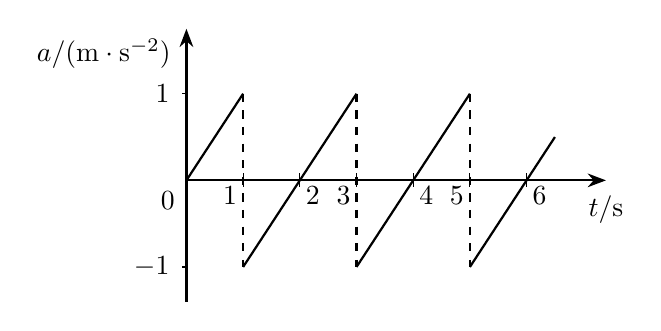
\begin{tikzpicture}[>=Stealth, x=0.72cm, y=1.1cm]
  % Axes
  \draw[->, thick] (0,0) -- (7.4,0) node[below=2pt] {$t/\mathrm{s}$};
  \draw[->, thick] (0,-1.4) -- (0,1.75) node[left=2pt, anchor=north east] {$a/(\mathrm{m\cdot s^{-2}})$};

  % Origin and y-axis ticks
  \node[below left=1pt] at (0,0) {$0$};
  \draw (0,1) -- (-0.08,1) node[left=1pt] {$1$};
  \draw (0,-1) -- (-0.08,-1) node[left=1pt] {$-1$};

  % x-axis ticks and labels
  \foreach \x in {1,3,5} {
    \draw (\x, 0.08) -- (\x, -0.08);
    \node[anchor=north east, inner sep=2pt] at (\x, 0) {$\x$};
  }
  \foreach \x in {2,4,6} {
    \draw (\x, 0.08) -- (\x, -0.08);
    \node[anchor=north west, inner sep=2pt] at (\x, 0) {$\x$};
  }

  % Sawtooth acceleration curve
  \draw[thick] (0,0) -- (1,1);
  \draw[dashed, thick] (1,1) -- (1,-1);
  \draw[thick] (1,-1) -- (3,1);
  \draw[dashed, thick] (3,1) -- (3,-1);
  \draw[thick] (3,-1) -- (5,1);
  \draw[dashed, thick] (5,1) -- (5,-1);
  \draw[thick] (5,-1) -- (6.5,0.5);
\end{tikzpicture}
\end{center}
\end{problem}
\clearpage


\begin{problem}{1.1.6}
一质点以恒定的径向速度分量 $\dot{r} = 4\mathrm{m}\cdot \mathrm{s}^{-1}$ 、横向速度分量与矢径成正比，比例系数为 $3\mathrm{rad / s}$ ，在一平面内运动。当质点离出发点 $4\mathrm{m}$ 时，它的速度及加速度的大小为何值？
\end{problem}
\clearpage


\begin{problem}{1.1.7}
质点的运动学方程为：(1) $r = (4t + 5t^2)i - 5j$ ；(2) $r = (2 + 3t)i - (2t - 3t^2)j$ . 求两运动的轨迹.
\end{problem}
\clearpage


\begin{problem}{1.1.8}
一质点沿直线运动, 其速度为 $v = A t - B x$ , 其中 $A, B$ 均为常数. 当 $t = 0$ 时, $x = 0$ . 试求位置坐标与 $t$ 的函数关系式及 $t = 0$ 时的加速度 $a_0$ .
\end{problem}
\clearpage


\begin{problem}{1.1.9}
某固体燃料火箭的垂直加速度为

\[
a = k \mathrm{e} ^ {- b t} - c v - g
\]

式中 b、c、k 均为常数，v 是获得的垂直速度，g 是重力加速度。在大气中运行时，g 被视为常量。试求火箭发射后 t 秒时的垂直速度。
\end{problem}
\clearpage


\begin{problem}{1.1.10}
图 1.2 中机构包括一根固定的弯成曲线的杆和一根用轴钉可绕 O 点转动的动杆 OC。弯杆曲线的方程为 $r=20\sin2\varphi$ 。木块 A 和 B 钉在一起，A、B 分别沿弯杆和直杆 OC 滑动。若 OC 以恒定角速度 5rad/s 做逆时针转动。求木块 A、B 在 r=10cm 处时的速度和加速度。
\begin{center}
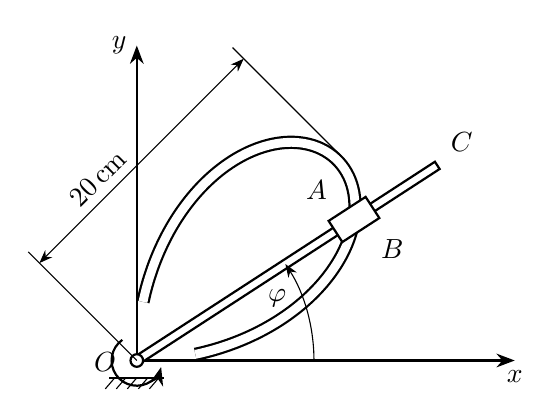
\begin{tikzpicture}[>=Stealth, scale=1]
  % Coordinate axes
  \draw[->, thick] (0,0) -- (4.8,0) node[below] {$x$};
  \draw[->, thick] (0,0) -- (0,4.0) node[left] {$y$};

  % Ground hatching under pivot O
  \draw[thick] (-0.35,-0.22) -- (0.35,-0.22);
  \foreach \x in {-0.28,-0.14,0,0.14,0.28} {
    \draw (\x,-0.22) -- (\x-0.12,-0.36);
  }
  \node[left=4pt] at (0,-0.02) {$O$};

  % Rotation arrow around O
  \draw[->, thick] (125:0.32) arc (125:345:0.32);

  % Curved rod r = 20 sin(2 phi), scaled so 20 cm = 3.6 cm, uniform hollow tube
  \draw[thick, double=white, double distance=3.2pt, samples=90, smooth, domain=6:84]
    plot (\x:{3.6*sin(2*\x)});

  % Straight rod OC at phi = 33 deg
  \def\ang{33}
  \def\rlen{4.55}
  \draw[thick, fill=white]
    (0,0) ++(\ang+90:0.055) -- ++(\ang:\rlen) -- ++(\ang-90:0.11) -- ++(\ang+180:\rlen) -- cycle;

  % Hinge circle at O
  \draw[thick, fill=white] (0,0) circle (0.08);

  % Slider block A-B at intersection r = 3.6 * sin(2*33)
  \pgfmathsetmacro{\rmid}{3.6*sin(2*\ang)}
  \begin{scope}[shift={(\ang:\rmid)}, rotate=\ang]
    \draw[thick, fill=white] (-0.28,-0.16) rectangle (0.28,0.16);
    \node[above left=2pt] at (-0.1,0.16) {$A$};
    \node[below right=2pt] at (0.1,-0.16) {$B$};
  \end{scope}

  % Label C at rod end
  \node[above right=2pt] at (\ang:\rlen) {$C$};

  % Angle phi arc and label in clear open space
  \draw[->] (2.25,0) arc (0:\ang:2.25);
  \node at (24:1.95) {$\varphi$};

  % Dimension line for 20 cm along 45 deg
  \coordinate (Peak) at (45:3.67);
  \draw[thin] (0,0) -- (135:1.95);
  \draw[thin] (Peak) -- ++(135:1.95);
  \draw[<->, thin] (135:1.75) -- node[above left, sloped] {$20\,\mathrm{cm}$} ($(Peak)+(135:1.75)$);
\end{tikzpicture}
\end{center}
\end{problem}
\clearpage


\begin{problem}{1.1.11}
质点以恒定速率 v 沿图示的半径为 R 的圆形轨道运动, 用图 1.3 示的极坐标写出质点在 $0 \leqslant \varphi \leqslant 2\pi$ 的各个位置时的速度和加速度.
\begin{center}
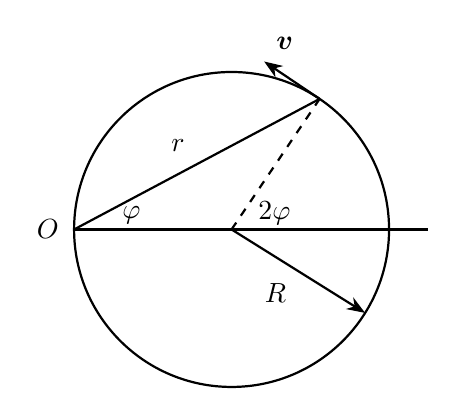
\begin{tikzpicture}[>=Stealth, scale=1]
  \def\R{2.0}
  \def\phiang{28}
  \coordinate (O) at (-\R, 0);
  \coordinate (C) at (0, 0);
  \coordinate (P) at ({2*\phiang}:\R);

  % Circle
  \draw[thick] (C) circle (\R);

  % Polar axis from O through C past right edge
  \draw[thick] (O) -- (\R+0.5, 0);
  \node[left=2pt] at (O) {$O$};

  % Chord r from O to P
  \draw[thick] (O) -- (P) node[midway, above left=1pt] {$r$};

  % Dashed radius from C to P
  \draw[dashed, thick] (C) -- (P);

  % Solid radius arrow R
  \draw[->, thick] (C) -- (-32:\R) node[midway, below left=1pt] {$R$};

  % Tangent velocity vector v at P
  \draw[->, thick] (P) -- ++({2*\phiang+90}:0.85) node[above right=1pt] {$\boldsymbol{v}$};

  % Angle labels
  \node at ($(O)+(\phiang/2:0.75)$) {$\varphi$};
  \node at ($(C)+(0.72*\phiang:0.58)$) {$2\varphi$};
\end{tikzpicture}
\end{center}
\end{problem}
\clearpage


\begin{problem}{1.1.12}
一质点沿心脏线 $r = 2(1 + \cos \varphi)$ 运动，在 $0 < \varphi < 180^{\circ}$ 期间， $\dot{r} = -2$ 。求在此期间质点的速度和加速度。
\end{problem}
\clearpage


\begin{problem}{1.1.13}
对于上题所述的质点运动,求速度平行于 x 轴时的 $\varphi$ 值及在此位置时的速度、加速度的大小.
\end{problem}
\clearpage


\begin{problem}{1.1.14}
离水面高度为 h 的岸上用绳索拉船靠岸, 人以恒定的速率 $v_{0}$ 拉绳, 将船的速度、加速度表示成船离岸的水平距离 L 的函数.
\end{problem}
\clearpage


\begin{problem}{1.1.15}
杆以匀角速 $\omega_{0}$ 绕过其固定端 O 且垂直于杆的轴转动，在 t=0 时，位于 O 点的小珠从相对于杆静止开始沿杆做相对于杆的加速度为 $a_{0}$ 的匀加速运动。求小珠相对于静系的速度、加速度与时间的关系。
\end{problem}
\clearpage


\begin{problem}{1.1.16}
在同一竖直面内的同一水平线上的 A、B 两点分别以 $30^{\circ}$ 、 $60^{\circ}$ 为发射角同时抛出两小球，欲使两小球相遇时都在自己轨道的最高点，已知在 A 点发射的小球发射速率 $v_{AO}=9.8m/s$ ，求 A、B 两点之间的距离 L.
\end{problem}
\clearpage


\begin{problem}{1.1.17}
在小丘上置一靶子，在炮位所在处看靶子的仰角为 $\alpha$ ，炮与靶子间的水平距离为 $L$ ，向目标射击时炮身的仰角为 $\beta$ ，炮弹以什么初速度发射才能击中目标？
\end{problem}
\clearpage


\begin{problem}{1.1.18}
一质点以恒定速率 v=c 沿悬链线

\[
y = \frac {a}{2} \left(\mathrm{e} ^ {\frac {x}{a}} + \mathrm{e} ^ {- \frac {x}{a}}\right)
\]

(其中 a 为正值常数)运动, t=0 时 x=0, 且沿 x 轴负向运动. 求位矢、速度、加速度随时间变化的关系.
\end{problem}
\clearpage


\begin{problem}{1.1.19}
某质点做平面运动, 其径向速度分量 $\dot{r} = c_{1}$ , 横向速度分量 $r\dot{\varphi} = c_{2}, c_{1}, c_{2}$ 均为正值常量. $t = 0$ 时加速度的横向分量 $a_{\varphi} = \frac{c_{1}c_{2}}{b}$ , $b$ 为正值常量, $\varphi = 0$ . 求运动学方程和 $t = 0$ 时加速度的径向分量.
\end{problem}
\clearpage


\begin{problem}{1.1.20}
在 t=0 时,从一点同时以同样大的速率 $v_{0}$ 向各个方向抛出小球.证明:在任一时刻 t,这些小球都位于一个球面上,球的中心以自由落体的加速度下落,球的半径等于 $v_{0}t$ .
\end{problem}
\clearpage


\begin{problem}{1.1.21}
已知一质点做平面运动, 其速率为常量 $c$ , 矢径的角速度的大小为常数 $\omega$ . 求该质点的运动学方程及其轨道. 设 $t=0$ 时, $r=0, \varphi=0$ .
\end{problem}
\clearpage


\begin{problem}{1.1.22}
如图 1.5, 一个动靶以恒定速率 v 在 xy 平面内沿 y=h 的直线飞行, t=0 时在 x=0、y=h 点. 导弹在 t=0 时自原点出发, 以恒定的速率 2v 运动, 速度方向始终指向动靶. 求导弹的运动轨道及导弹击中飞靶的时间.
\begin{center}
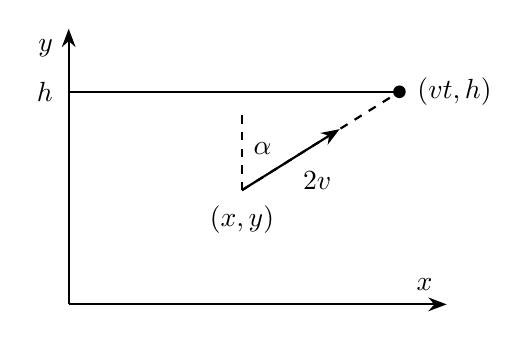
\begin{tikzpicture}[>=Stealth, scale=1]
  % Axes
  \draw[->, thick] (0,0) -- (4.8,0) node[above left=2pt] {$x$};
  \draw[->, thick] (0,0) -- (0,3.5) node[left=2pt, anchor=north east] {$y$};

  % Target path y = h and target dot
  \draw[thick] (0,2.7) node[left=2pt] {$h$} -- (4.2,2.7);
  \fill (4.2,2.7) circle (0.08);
  \node[right=3pt] at (4.2,2.7) {$(vt, h)$};

  % Missile position (x,y) and velocity vector
  \coordinate (M) at (2.2, 1.45);
  \coordinate (T) at (4.2, 2.7);
  \draw[dashed, thick] (M) -- (2.2, 2.5);
  \draw[dashed, thick] (M) -- (T);
  \draw[->, thick] (M) -- ($(M)!0.62!(T)$) node[midway, below right=1pt] {$2v$};

  \node[below=2pt] at (M) {$(x,y)$};
  \node at (2.46, 1.98) {$\alpha$};
\end{tikzpicture}
\end{center}
\end{problem}
\clearpage


\begin{problem}{1.1.23}
火车能达到的最大加速度为 $\alpha$ ，最大减速度为 $\beta$ 。求从静止出发到最后静止通过的距离 $a$ 和所需的最短时间。
\end{problem}
\clearpage


\begin{problem}{1.1.24}
直线 LM 在一给定的半径为 R 的圆平面内以等角速 $\omega$ 绕圆周上一点 A 转动. 求此直线与圆的另一交点 B 的速度和加速度的大小见图 1.7.
\begin{center}
\begin{tikzpicture}[>=Stealth, scale=1]
  \def\R{2.0}
  \def\phiang{42}
  \coordinate (O) at (0,0);
  \coordinate (Lend) at (-\R,0);
  \coordinate (Rend) at (\R,0);
  \coordinate (A) at (235:\R);
  \coordinate (B) at (\phiang:\R);

  % Circle
  \draw[thick] (O) circle (\R);

  % Base axis (基轴) and dashed left radius
  \draw[dashed, thick] (Lend) -- (O);
  \draw[thick] (O) -- (\R+0.8, 0) node[below=2pt] {\small 基轴};
  \node[below left=1pt] at (O) {$O$};
  \node[below=2pt] at (0.85, 0) {$R$};

  % Dashed chord from leftmost point to B
  \draw[dashed, thick] (Lend) -- (B);

  % Radius vector OB
  \draw[->, thick] (O) -- (B);
  \node[right=3pt] at (B) {$B$};

  % Angle phi arc
  \draw[->] (1.05,0) arc (0:\phiang:1.05);
  \node at (0.5*\phiang:1.28) {$\varphi$};

  % Line LM at t=0 passing through A and (R,0)
  \draw[thick] ($(A)!-0.45!(Rend)$) -- ($(A)!1.38!(Rend)$);
  \coordinate (Pzero) at ($(A)!0.48!(Rend)$);
  \draw[<-, thick] ($(Pzero)+(-60:0.15)$) -- ++(-60:0.65) node[below right=-2pt] {\small $t=0$ 时的 $LM$};

  % Current line LM passing through A and B
  \draw[thick] ($(A)!-0.32!(B)$) node[below right=1pt] {$L$} -- ($(A)!1.38!(B)$) node[above left=1pt] {$M$};
  \node[below right=2pt] at (A) {$A$};

  % Angles psi
  \node at ($(Lend)+(10:1.12)$) {$\psi$};
  \node at ($(A)+(38:1.25)$) {$\psi$};
\end{tikzpicture}
\end{center}
\end{problem}
\clearpage


\begin{problem}{1.1.25}
质点沿一平面做曲线运动, 其加速度矢量的作用线在任何时刻都通过一固定点 O. 试证明: 质点加速度的大小为 $a = \pm v \frac{dv}{dr}$ , 其中 v 为质点的速率, r 为质点到 O 点的距离, $\frac{dv}{dr} > 0$ 时取正号, $\frac{dv}{dr} < 0$ 时取负号.
\end{problem}
\clearpage


\section{自然坐标、切向加速度和法向加速度}

\begin{problem}{1.2.1}
一质点静止在半径为 $R$ 的半球面上的最高点. 要使质点脱离半球, 一开始就不沿半球滑下, 必须给予质点的最小水平速度多大?
\end{problem}
\clearpage


\begin{problem}{1.2.2}
一质点的运动学方程为

\[
\begin{array}{l} x = R \sin \omega t + \omega R t, \\ y = R \cos \omega t + R, \end{array}
\]

式中 $\omega, R$ 均为常量. 求质点在 y 的最大值、最小值时的切向加速度、法向加速度和轨道的曲率半径.
\end{problem}
\clearpage


\begin{problem}{1.2.3}
一质点沿抛物线 $y = \frac{1}{2} Ax^2$ 运动，设路程从抛物线顶点开始计算，质点运动的路程与时间的关系为 $s = bt^2 + ct, A, b, c$ 均是正值常量，试求在顶点时质点的切向加速度和法向加速度.
\end{problem}
\clearpage


\begin{problem}{1.2.4}
曲柄 $OA = r$ ，绕定轴 $O$ 以匀角速 $\omega$ 转动，连杆 $AB$ 用铰链与曲柄端点 $A$ 连接，并可在具有铰链的滑套 $N$ 内滑动。当 $\varphi = 0$ 时， $A$ 端位于滑套 $N$ 处。已知 $AB = l > 2r$ ，求当 $\varphi = 0$ 时，连杆上 $B$ 点的速度、加速度的大小，切向加速度、法向加速度和轨道的曲率半径（见图1.8）。
\begin{center}
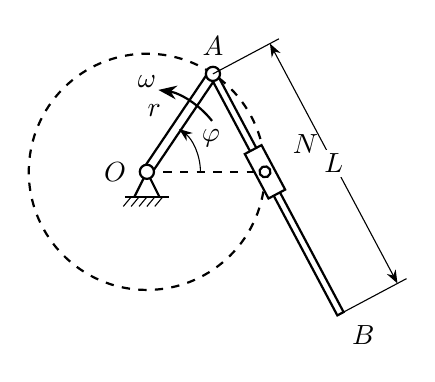
\begin{tikzpicture}[>=Stealth, scale=1]
  \def\r{1.5}
  \def\phiang{56}
  \coordinate (O) at (0,0);
  \coordinate (A) at (\phiang:\r);
  \coordinate (N) at (\r,0);
  % Direction from A to N
  \pgfmathsetmacro{\dx}{\r - \r*cos(\phiang)}
  \pgfmathsetmacro{\dy}{0 - \r*sin(\phiang)}
  \pgfmathsetmacro{\rodang}{atan2(\dy,\dx)}
  \def\Llen{3.45}
  \coordinate (B) at ($(A)+(\rodang:\Llen)$);

  % Dashed circle of radius r
  \draw[dashed, thick] (O) circle (\r);
  \draw[dashed, thick] (O) -- (N);

  % Ground support under O
  \draw[thick] (-0.28,-0.32) -- (0.28,-0.32);
  \foreach \x in {-0.2,-0.1,0,0.1,0.2} {
    \draw (\x,-0.32) -- (\x-0.1,-0.44);
  }
  \draw[thick] (-0.16,-0.32) -- (O) -- (0.16,-0.32);
  \node[left=4pt] at (O) {$O$};

  % Crank OA (double-line bar)
  \draw[thick, fill=white]
    (O) ++(\phiang+90:0.06) -- ($(A)+(\phiang+90:0.06)$) -- ($(A)+(\phiang-90:0.06)$) -- ($(O)+(\phiang-90:0.06)$) -- cycle;
  \node[above left=2pt] at ($0.42*(O)+0.42*(A)$) {$r$};

  % Connecting rod AB (double-line bar)
  \draw[thick, fill=white]
    (A) ++(\rodang+90:0.045) -- ($(B)+(\rodang+90:0.045)$) -- ($(B)+(\rodang-90:0.045)$) -- ($(A)+(\rodang-90:0.045)$) -- cycle;

  % Hinge pins at O and A
  \draw[thick, fill=white] (O) circle (0.09);
  \draw[thick, fill=white] (A) circle (0.09);
  \node[above=3pt] at (A) {$A$};
  \node[below right=1pt] at (B) {$B$};

  % Slider sleeve N
  \begin{scope}[shift={(N)}, rotate=\rodang]
    \draw[thick, fill=white] (-0.32,-0.12) rectangle (0.32,0.12);
    \draw[thick] (0,0) circle (0.07);
  \end{scope}
  \node[above right=2pt] at ($(N)+(0.18,0.06)$) {$N$};

  % Angle phi and angular velocity omega
  \draw[->] (0.68,0) arc (0:\phiang-3:0.68);
  \node at (0.5*\phiang:0.92) {$\varphi$};
  \draw[->, thick] (\phiang-18:1.05) arc (\phiang-18:\phiang+26:1.05);
  \node at (\phiang+34:1.14) {$\omega$};

  % Dimension L
  \draw[thin] (A) -- ++(\rodang+90:0.95);
  \draw[thin] (B) -- ++(\rodang+90:0.95);
  \draw[<->, thin] ($(A)+(\rodang+90:0.82)$) -- node[fill=white, inner sep=1.5pt] {$L$} ($(B)+(\rodang+90:0.82)$);
\end{tikzpicture}
\end{center}
\end{problem}
\clearpage


\begin{problem}{1.2.5}
质点 $P$ 沿一平面曲线运动, 其加速度矢量的作用线与曲率圆交于 $A$ 点, $PA$ 间距离为 $l$ . 试证: 质点的加速度大小为 $a = \frac{2v^2}{l}$ , 其中 $v$ 是质点的速率.
\end{problem}
\clearpage


\begin{problem}{1.2.6}
某个在平面上运动的质点, 其速度的 $y$ 分量 $\dot{y} = c$ 为常量. 试证其加速度值 $a = \frac{v^3}{c\rho}$ , 式中 $v$ 为速率, $\rho$ 为曲率半径.
\end{problem}
\clearpage


\begin{problem}{1.2.7}
一质点的运动轨道为对数螺旋线 $r = b\mathrm{e}^{k\varphi}$ , 其中 $b, k$ 均为正值常量, $\dot{r} = c$ ( $c$ 为正值常量), $t = 0$ 时, 位于 $r = b, \varphi = 0$ 处. 求质点的速度和加速度的大小以及曲率半径随时间的变化规律.
\end{problem}
\clearpage


\begin{problem}{1.2.8}
质点做平面运动,轨道方程为 $y=y(x)$ ,试证:

\[
\rho = \frac {(1 + y ^ {\prime 2}) ^ {3 / 2}}{| y ^ {\prime \prime} |}
\]

式中 $\rho$ 为曲率半径， $y' = \frac{\mathrm{d}y}{\mathrm{d}x}, y'' = \frac{\mathrm{d}^2y}{\mathrm{d}x^2}$ .
\end{problem}
\clearpage


\begin{problem}{1.2.9}
已知质点的运动轨道为 $r = r(\varphi), (r, \varphi$ 为极坐标)，求轨道上各点的曲率半径.
\end{problem}
\clearpage


\begin{problem}{1.2.10}
求 1.1.10 题所述轨道在 r=10cm 处的曲率半径.
\end{problem}
\clearpage


\section{质点的相对运动}

\begin{problem}{1.3.1}
一直升飞机在离地面 $4.9\mathrm{m}$ 的高度以 $4.9\mathrm{m / s}$ 的恒定水平速度飞行，一包裹从直升飞机上沿水平方向丢出时相对于直升飞机的初速度为 $12\mathrm{m / s}$ ，方向与飞行方向相反。求：

(1) 当包裹落到地面时, 它与直升飞机的水平距离;

(2) 包裹刚要着地时其速度矢量与地面的夹角.
\end{problem}
\clearpage


\begin{problem}{1.3.2}
一列火车在刮着北风的雨中以 $30\mathrm{m / s}$ 的速率(相对于地面)向正南方行驶。一在地面上静止的观察者测得雨滴的路径与竖直线成 $25^{\circ}$ 角，火车中的观察者看到雨水在车窗玻璃上的径迹是竖直向下的。求雨滴相对于地面的速率。
\end{problem}
\clearpage


\begin{problem}{1.3.3}
一架飞机在静止空气中的速率为 60m/s，风的速率为 30m/s，飞机仍能向北以 60m/s 的速率飞行。求：(1) 风向；(2) 机头的指向。
\end{problem}
\clearpage


\begin{problem}{1.3.4}
一飞机带的燃料, 在无风的情况下, 以 $v$ 的速率飞行, 可飞行来回的总路程为 $R$ . 今在有风的情况下, 要向北偏东 $\varphi^{\circ}$ 角的方向去执行任务, 并飞回基地. 若风向为北偏东 $\alpha^{\circ}$ , 风速为 $\bm{u}$ . 问该机能飞离基地多大距离?
\end{problem}
\clearpage


\begin{problem}{1.3.5}
蒸汽轮船以 $v_{1}$ 的速度向南航行, 船上的人看到烟囱中冒出的烟向东方向, 若船速增至 $v_{2}$ , 船上的人看到烟向东北, 若烟从烟囱冒出后立即按风速运动, 求风速.
\end{problem}
\clearpage


\begin{problem}{1.3.6}
一个小环 $M$ 同时套在两根细棒上，棒 $AB$ 以速度 $\bm{v}_{1}$ 沿垂直于 $AB$ 的方向移动，棒 $CD$ 以速度 $\bm{v}_{2}$ 沿垂直于 $CD$ 的方向移动，两棒始终处在同一平面上，两棒夹角为 $\alpha$ ，如图1.13所示.求小环 $M$ 的速度.
\begin{center}
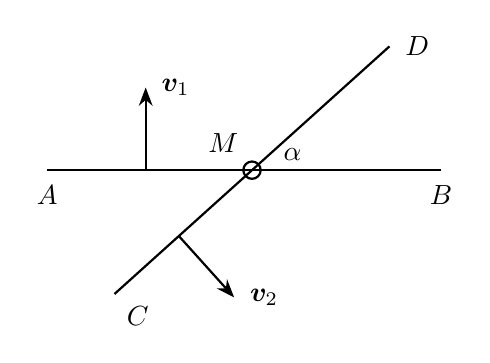
\begin{tikzpicture}[>=Stealth, scale=1]
  \def\ang{42}
  % Rod AB
  \draw[thick] (-2.6,0) node[below=2pt] {$A$} -- (2.4,0) node[below=2pt] {$B$};

  % Rod CD
  \draw[thick] (180+\ang:2.35) node[below right=1pt] {$C$} -- (\ang:2.35) node[right=2pt] {$D$};

  % Ring M at intersection (0,0)
  \draw[thick] (0,0) circle (0.11);
  \node[above left=2pt] at (0,0.05) {$M$};

  % Angle alpha
  \node at (0.5*\ang:0.55) {$\alpha$};

  % Velocity vectors
  \draw[->, thick] (-1.35,0) -- (-1.35,1.05) node[right=2pt] {$\boldsymbol{v}_1$};
  \coordinate (Q) at (180+\ang:1.25);
  \draw[->, thick] (Q) -- ++(\ang-90:1.05) node[right=2pt] {$\boldsymbol{v}_2$};
\end{tikzpicture}
\end{center}
\end{problem}
\clearpage


\begin{problem}{1.3.7}
圆心为 A、B，半径均为 R=5cm 的两个大圆环处在同一平面上。B 环固定，A

环沿着 $AB$ 连线向 $B$ 环运动. 另有一小环 $M$ 同时套在两个大圆环上. 当 $A$ 环运动到 $\alpha = 30^{\circ}$ 时, $A$ 点的速度 $v_{A} = 5\mathrm{cm}\cdot \mathrm{s}^{-1}$ , 加速度 $a_{A} = 0$ . 求此时小环 $M$ 的速度和加速度的大小.
\end{problem}
\clearpage


\begin{problem}{1.3.8}
有一与 $x$ 轴夹角为 $45^{\circ}$ 的直线，以速率 $u$ 垂直于直线的方向向 $x$ 轴负向、 $y$ 轴正向运动。设在 $t = 0$ 时，它与悬链线

\[
y = \frac {a}{2} \left(\mathrm{e} ^ {\frac {x}{a}} + \mathrm{e} ^ {- \frac {x}{a}}\right)
\]

(其中 a 为正值常数)交于 x=0 处, 求此交点的速度作为时间的函数. 另一个交点移动的速度又如何随时间变化?
\end{problem}
\clearpage


\begin{problem}{1.3.9}
用相对运动理论求 1.1.24 题中 B 点相对于直线 LM 的速度和加速度.
\end{problem}
\clearpage


\begin{problem}{1.3.10}
一个半径为 $R$ 的转盘绕通过盘心的垂直盘面的轴以恒定角速度 $\omega$ 转动。两个小孩 $A$ 和 $B$ 相对于圆盘静止于盘的边缘， $\angle AOB = 90^{\circ}$ ，用图画出在图1.18所示位置， $A$ 看到的 $B$ 的速度和加速度，标明大小和方向，分别选用以 $A$ 为原点的平动参考系和转动参考系。
\begin{center}
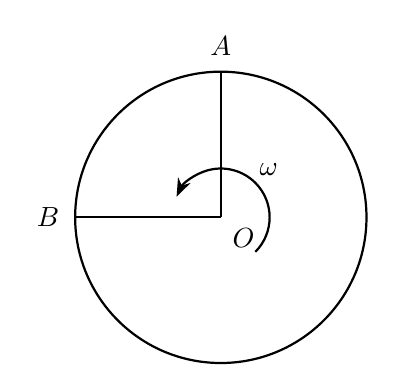
\begin{tikzpicture}[>=Stealth, scale=1]
  \def\R{1.85}
  \coordinate (O) at (0,0);
  \coordinate (A) at (0,\R);
  \coordinate (B) at (-\R,0);

  % Disk
  \draw[thick] (O) circle (\R);

  % Radii OA and OB
  \draw[thick] (O) -- (A) node[above=2pt] {$A$};
  \draw[thick] (O) -- (B) node[left=2pt] {$B$};
  \node[below right=1pt] at (O) {$O$};

  % Counterclockwise angular velocity arrow omega
  \draw[->, thick] (-45:0.62) arc (-45:155:0.62);
  \node at (45:0.86) {$\omega$};
\end{tikzpicture}
\end{center}
\end{problem}
\clearpage


\begin{problem}{1.3.12}
平面 I 可绕通过固定点 $O_{1}$ (在平面 I 上) 的垂直轴转动, 平面 II 可绕通过 $O_{2}$ (固连于平面 I) 的垂直于两平面的轴转动. 若 $\omega_{1} = \omega_{2}$ , 如图 1.23 所示. 证明在静参考系中平面 II 作平动.

提示: 只要证明平面 Ⅱ 上任一点 A 的绝对速度与 A 的位置无关即可.
\begin{center}
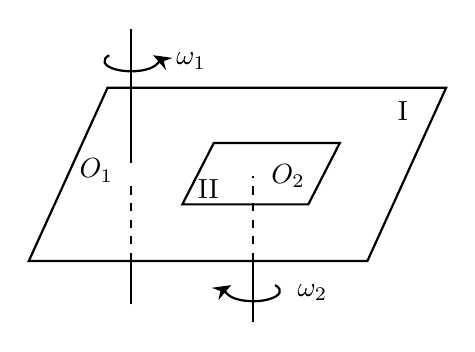
\begin{tikzpicture}[>=Stealth, scale=1]
  % Plane I
  \draw[thick] (0,0) -- (4.3,0) -- (5.3,2.2) -- (1.0,2.2) -- cycle;
  \node at (4.75, 1.9) {$\mathrm{I}$};

  % Plane II (smaller parallelogram on top of I)
  \draw[thick, fill=white] (1.95,0.72) -- (3.55,0.72) -- (3.95,1.5) -- (2.35,1.5) -- cycle;
  \node at (2.28, 0.92) {$\mathrm{II}$};

  % Axis O1
  \draw[thick] (1.3, 1.25) -- (1.3, 2.95);
  \draw[dashed, thick] (1.3, 0) -- (1.3, 1.05);
  \draw[thick] (1.3, -0.55) -- (1.3, 0);
  \node[left=3pt] at (1.3, 1.15) {$O_1$};

  % Rotation arrow omega1 (counterclockwise viewed from above, centered on axis x=1.3)
  \draw[->, thick] ([shift=(145:0.34 and 0.13)]1.3, 2.54) arc (145:395:0.34 and 0.13);
  \node[right=2pt] at (1.68, 2.54) {$\omega_1$};

  % Axis O2
  \draw[dashed, thick] (2.85, 0) -- (2.85, 1.08);
  \draw[thick] (2.85, -0.78) -- (2.85, 0);
  \node[right=3pt] at (2.85, 1.08) {$O_2$};

  % Rotation arrow omega2 (opposite sense: clockwise viewed from above, centered on axis x=2.85)
  \draw[->, thick] ([shift=(35:0.34 and 0.13)]2.85, -0.38) arc (35:-215:0.34 and 0.13);
  \node[right=2pt] at (3.22, -0.40) {$\omega_2$};
\end{tikzpicture}
\end{center}
\end{problem}
\clearpage


\begin{problem}{1.3.13}
一个质点在 $xy$ 平面内的运动学方程为 $x = f(t), y = g(t)$ ，此平面以等角速 $\omega$ 绕过原点在 $xz$ 平面上与 $x, z$ 轴的夹角均为 $45^{\circ}$ 的固定轴转动。求质点对静参考系的速度和加速度（用动坐标系表达）。
\end{problem}
\clearpage


\begin{problem}{1.3.14}
一个质点在 $xy$ 平面内的运动学方程为 $r = \mathrm{e}^{ct}, \varphi = bt(c, b$ 为常量), $r, \varphi$ 为极坐标. 此平面以等角速 $\omega$ 绕固定的 $x$ 轴转动. 求质点的绝对速度和绝对加速度 (见图1.25).
\begin{center}
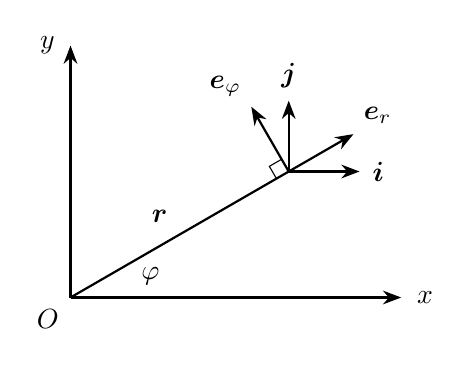
\begin{tikzpicture}[>=Stealth, scale=1]
  \def\ang{30}
  \def\rlen{3.2}
  \coordinate (O) at (0,0);
  \coordinate (P) at (\ang:\rlen);

  % Axes
  \draw[->, thick] (O) -- (4.2,0) node[right=2pt] {$x$};
  \draw[->, thick] (O) -- (0,3.2) node[left=2pt] {$y$};
  \node[below left=1pt] at (O) {$O$};

  % Position vector line r
  \draw[thick] (O) -- (P) node[midway, above left=1pt] {$\boldsymbol{r}$};
  \node at (0.5*\ang:1.05) {$\varphi$};

  % Unit vectors at P
  \draw[->, thick] (P) -- ++(0.9, 0) node[right=1pt] {$\boldsymbol{i}$};
  \draw[->, thick] (P) -- ++(0, 0.9) node[above=1pt] {$\boldsymbol{j}$};
  \draw[->, thick] (P) -- ++(\ang:0.95) node[above right=0pt] {$\boldsymbol{e}_r$};
  \draw[->, thick] (P) -- ++(\ang+90:0.95) node[above left=0pt] {$\boldsymbol{e}_\varphi$};

  % Right-angle mark between OP and e_phi
  \draw[thin] ($(P)+(\ang+180:0.18)$) -- ++(\ang+90:0.18) -- ++(\ang:0.18);
\end{tikzpicture}
\end{center}
\end{problem}
\clearpage


\begin{problem}{1.3.15}
图 1.26 中机构在图示位置时, 杆 OA 绕 O 点的角速度为 2rad/s, 求此时 C 的角速度 $\omega$ 及 B 点的速度 $v_{B}$ .
\begin{center}
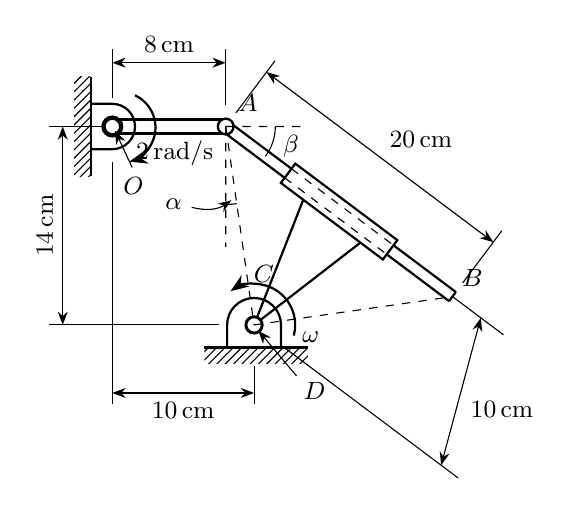
\begin{tikzpicture}[>=Stealth, scale=0.18, every node/.style={font=\small}]
  % Coordinates (1 unit = 1 cm in problem, scaled by 0.18 -> ~5.8 cm wide)
  \coordinate (O) at (0, 14);
  \coordinate (A) at (8, 14);
  \coordinate (D) at (10, 0);
  \coordinate (B) at (24, 2);

  % Wall at O
  \draw[thick] (-1.5, 10.5) -- (-1.5, 17.5);
  \fill[pattern=north east lines] (-2.7, 10.5) rectangle (-1.5, 17.5);
  % Bearing bracket at O
  \draw[thick] (-1.5, 15.6) -- (0, 15.6) arc (90:-90:1.6) -- (-1.5, 12.4);
  \draw[thick, fill=white] (O) circle (0.7);

  % Crank OA (double-line bar)
  \draw[thick] (0, 14.5) -- (8, 14.5);
  \draw[thick] (0, 13.5) -- (8, 13.5);
  \draw[thick, fill=white] (O) circle (0.55);
  \draw[thick, fill=white] (A) circle (0.55);

  % Angular velocity arrow around OA
  \draw[->, thick] (1.6, 16.2) arc (65:-75:2.5);
  \node at (4.4, 12.1) {$2\,\mathrm{rad/s}$};

  % Ground and bearing bracket at D
  \draw[thick] (6.5, -1.6) -- (13.8, -1.6);
  \fill[pattern=north east lines] (6.5, -2.7) rectangle (13.8, -1.6);
  \draw[thick] (8.1, -1.6) -- (8.1, 0) arc (180:0:1.9) -- (11.9, -1.6);
  \draw[thick, fill=white] (D) circle (0.6);

  % Rod AB and sliding sleeve C
  % Direction of AB: angle -36.87 deg (cos=0.8, sin=-0.6)
  % Sleeve spans from s=5.5 to s=14.5 along AB
  \coordinate (S1) at ($(A)!0.275!(B)$);
  \coordinate (S2) at ($(A)!0.725!(B)$);
  \coordinate (perp) at (0.6, 0.8); % unit normal to AB pointing up-right

  % Rod AB
  \draw[thick] ($(A)+0.4*(perp)$) -- ($(S1)+0.4*(perp)$);
  \draw[thick] ($(A)-0.4*(perp)$) -- ($(S1)-0.4*(perp)$);
  \draw[thick] ($(S2)+0.4*(perp)$) -- ($(B)+0.4*(perp)$);
  \draw[thick] ($(S2)-0.4*(perp)$) -- ($(B)-0.4*(perp)$);
  \draw[thick] ($(B)+0.4*(perp)$) -- ($(B)-0.4*(perp)$);

  % Sleeve around AB
  \draw[thick] ($(S1)+0.85*(perp)$) -- ($(S2)+0.85*(perp)$)
            -- ($(S2)-0.85*(perp)$) -- ($(S1)-0.85*(perp)$) -- cycle;
  \draw[dashed] ($(S1)+0.4*(perp)$) -- ($(S2)+0.4*(perp)$);
  \draw[dashed] ($(S1)-0.4*(perp)$) -- ($(S2)-0.4*(perp)$);
  \draw[thick, fill=white] (A) circle (0.55);

  % Rocker C arms from D to sleeve
  \coordinate (M1) at ($(S1)!0.22!(S2) - 0.85*(perp)$);
  \coordinate (M2) at ($(S1)!0.78!(S2) - 0.85*(perp)$);
  \draw[thick] (D) -- (M1);
  \draw[thick] (D) -- (M2);
  \draw[thick, fill=white] (D) circle (0.55);

  % Angular velocity arrow around D
  \draw[->, thick] ($(D)+(-15:2.9)$) arc (-15:125:2.9);
  \node at (10.7, 3.6) {$C$};
  \node at ($(D)+(-12:4.1)$) {$\omega$};

  % Dashed geometric lines
  \draw[dashed] (A) -- (13.5, 14); % horizontal right from A
  \draw[dashed] (A) -- (8, 5.5);   % vertical down from A
  \draw[dashed] (A) -- (D);        % AD
  \draw[dashed] (D) -- (B);        % DB

  % Angle arcs alpha and beta
  \draw (8, 8.5) arc (-90:-81.87:5.5);
  \draw[->] (5.6, 8.3) to[bend right=25] (8.4, 8.8);
  \node[left] at (5.6, 8.5) {$\alpha$};
  \draw (11.5, 14) arc (0:-36.87:3.5);
  \node at (12.6, 12.6) {$\beta$};

  % Dimension: 8 cm
  \draw (0, 16) -- (0, 19.5);
  \draw (8, 15.5) -- (8, 19.5);
  \draw[<->] (0, 18.5) -- node[above] {$8\,\mathrm{cm}$} (8, 18.5);

  % Dimension: 14 cm
  \draw (-4.5, 14) -- (-0.8, 14);
  \draw (-4.5, 0) -- (7.5, 0);
  \draw[<->] (-3.5, 0) -- node[left, rotate=90, anchor=south] {$14\,\mathrm{cm}$} (-3.5, 14);

  % Dimension: 10 cm (horizontal O to D)
  \draw (0, 11.5) -- (0, -5.6);
  \draw (10, -2.9) -- (10, -5.6);
  \draw[<->] (0, -4.8) -- node[below] {$10\,\mathrm{cm}$} (10, -4.8);

  % Dimension: 20 cm (parallel to AB)
  \draw ($(A)+1.2*(perp)$) -- ($(A)+5.8*(perp)$);
  \draw ($(B)+1.2*(perp)$) -- ($(B)+5.8*(perp)$);
  \draw[<->] ($(A)+4.8*(perp)$) -- node[above right, pos=0.5] {$20\,\mathrm{cm}$} ($(B)+4.8*(perp)$);

  % Dimension: 10 cm (perpendicular from D to line AB)
  \coordinate (D_ext) at ($(D) + 18*(0.8, -0.6)$);
  \coordinate (B_ext) at ($(B) + 4.5*(0.8, -0.6)$);
  \draw ($(D)+2.5*(0.8,-0.6)$) -- (D_ext);
  \draw (B) -- (B_ext);
  \draw[<->] ($(D) + 16.5*(0.8, -0.6)$) -- node[below right] {$10\,\mathrm{cm}$} ($(B) + 2.5*(0.8, -0.6)$);

  % Point labels
  \node[above right] at (8.2, 14.4) {$A$};
  \node[above right] at (B) {$B$};
  \draw[->] (1.4, 11.1) -- ($(O)+(0.2,-0.3)$);
  \node[below] at (1.5, 11.1) {$O$};
  \draw[->] (13.0, -3.6) -- ($(D)+(0.3,-0.4)$);
  \node[below right] at (12.8, -3.4) {$D$};
\end{tikzpicture}
\end{center}
\end{problem}
\clearpage


\begin{problem}{1.3.16}
若上题除所给条件以外再加上在图示位置 $OA$ 杆绕 $O$ 点的角加速度为零，求此时 $C$ 的角加速度 $\dot{\omega}$ 及 $B$ 点的加速度 $a_{B}$ .
\begin{center}
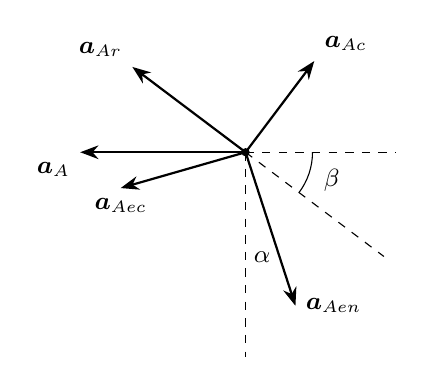
\begin{tikzpicture}[>=Stealth, every node/.style={font=\small}]
  \coordinate (O) at (0, 0);
  \fill (O) circle (1.5pt);

  % Dashed reference lines
  \draw[dashed] (O) -- (1.9, 0);
  \draw[dashed] (O) -- (-37:2.2);
  \draw[dashed] (O) -- (0, -2.6);

  % Angle labels
  \draw (0.85, 0) arc (0:-37:0.85);
  \node at (-18:1.15) {$\beta$};
  \node at (-81:1.35) {$\alpha$};

  % Acceleration vectors
  \draw[->, thick] (O) -- (-2.1, 0) node[below left] {$\boldsymbol{a}_{A}$};
  \draw[->, thick] (O) -- (143:1.8) node[above left] {$\boldsymbol{a}_{Ar}$};
  \draw[->, thick] (O) -- (53:1.45) node[above right] {$\boldsymbol{a}_{Ac}$};
  \draw[->, thick] (O) -- (-164:1.65) node[below] {$\boldsymbol{a}_{Aec}$};
  \draw[->, thick] (O) -- (-72:2.05) node[right] {$\boldsymbol{a}_{Aen}$};
\end{tikzpicture}
\end{center}
\end{problem}
\clearpage


\chapter{质点动力学}

\section{牛顿运动定律}

\begin{problem}{2.1.1}
质量为 $M$ 的人通过质量可以不计、不可伸长的绳子和摩擦可忽略的定滑轮，

将质量为 m 的重物提起, 如图 2.1 所示. 分两种情况: (1) 物

体匀速上升；(2)物体以加速度 $a$ 上升.求人对地面的压力.
\begin{center}
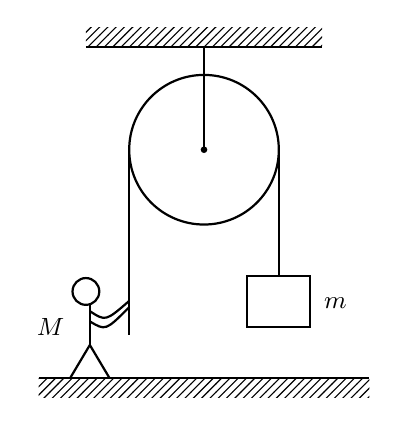
\begin{tikzpicture}[>=Stealth, every node/.style={font=\small}]
  % Ceiling
  \draw[thick] (-1.5, 4.2) -- (1.5, 4.2);
  \fill[pattern=north east lines] (-1.5, 4.2) rectangle (1.5, 4.45);

  % Pulley support & pulley
  \draw[thick] (0, 4.2) -- (0, 2.9);
  \draw[thick] (0, 2.9) circle (0.95);
  \fill (0, 2.9) circle (1.2pt);

  % Left rope and person M
  \draw[thick] (-0.95, 2.9) -- (-0.95, 0.55);
  % Stick figure
  \draw[thick] (-1.5, 1.1) circle (0.17);
  \draw[thick] (-1.45, 0.93) -- (-1.45, 0.42);
  \draw[thick] (-1.45, 0.42) -- (-1.7, 0);
  \draw[thick] (-1.45, 0.42) -- (-1.2, 0);
  \draw[thick] (-1.45, 0.85) .. controls (-1.25, 0.72) .. (-0.95, 0.98);
  \draw[thick] (-1.45, 0.72) .. controls (-1.25, 0.60) .. (-0.95, 0.90);
  \node[left] at (-1.65, 0.65) {$M$};

  % Right rope and hanging block m
  \draw[thick] (0.95, 2.9) -- (0.95, 1.3);
  \draw[thick] (0.55, 0.65) rectangle (1.35, 1.3);
  \node[right] at (1.4, 0.95) {$m$};

  % Ground
  \draw[thick] (-2.1, 0) -- (2.1, 0);
  \fill[pattern=north east lines] (-2.1, -0.25) rectangle (2.1, 0);
\end{tikzpicture}
\end{center}
\end{problem}
\clearpage


\begin{problem}{2.1.2}
图 2.2 中人的质量 $m_{1}=60kg$ ，人所站着的底板质量 $m_{2}=20kg$ ，绳子和滑轮质量均可忽略不计。人要用多大的力拉住绳子，才能保持自己和底板静止不动。
\begin{center}
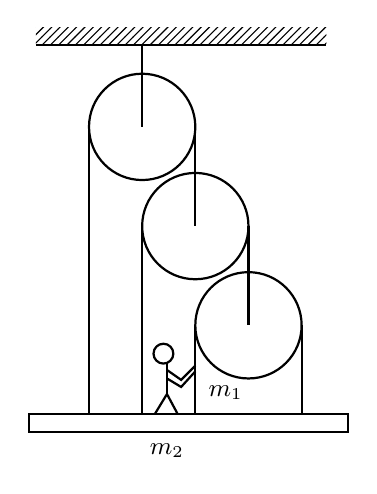
\begin{tikzpicture}[>=Stealth, scale=0.9, every node/.style={font=\small}]
  % Ceiling
  \draw[thick] (-1.5, 5.5) -- (2.6, 5.5);
  \fill[pattern=north east lines] (-1.5, 5.5) rectangle (2.6, 5.75);

  % Pulley 1 (top)
  \draw[thick] (0, 5.5) -- (0, 4.35);
  \draw[thick] (0, 4.35) circle (0.75);
  \draw[thick] (-0.75, 4.35) -- (-0.75, 0.3);
  \draw[thick] (0.75, 4.35) -- (0.75, 2.95);

  % Pulley 2 (middle)
  \draw[thick] (0.75, 2.95) circle (0.75);
  \draw[thick] (0, 2.95) -- (0, 0.3);
  \draw[thick] (1.5, 2.95) -- (1.5, 1.55);

  % Pulley 3 (bottom)
  \draw[thick] (1.5, 1.55) circle (0.75);
  \draw[thick] (0.75, 1.55) -- (0.75, 0.3);
  \draw[thick] (2.25, 1.55) -- (2.25, 0.3);

  % Person standing on platform holding left rope of Pulley 3
  \draw[thick] (0.3, 1.15) circle (0.14);
  \draw[thick] (0.35, 1.01) -- (0.35, 0.58);
  \draw[thick] (0.35, 0.58) -- (0.18, 0.3);
  \draw[thick] (0.35, 0.58) -- (0.50, 0.3);
  \draw[thick] (0.35, 0.92) -- (0.55, 0.78) -- (0.75, 0.98);
  \draw[thick] (0.35, 0.80) -- (0.55, 0.68) -- (0.75, 0.90);
  \node[right] at (0.8, 0.6) {$m_1$};

  % Platform
  \draw[thick] (-1.6, 0.05) rectangle (2.9, 0.3);
  \node[below] at (0.35, 0.02) {$m_2$};
\end{tikzpicture}
\end{center}
\end{problem}
\clearpage


\begin{problem}{2.1.3}
跨过一个无摩擦定滑轮的一根绳子,一端挂有9kg质量,另一端挂有7kg质量,如图2.3所示.求加速度和绳中的张力.

解得
\begin{center}
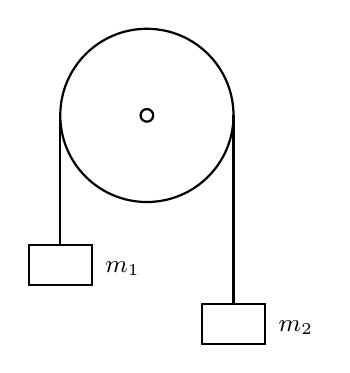
\begin{tikzpicture}[>=Stealth, every node/.style={font=\small}]
  % Pulley
  \draw[thick] (0, 3.0) circle (1.1);
  \draw[thick] (0, 3.0) circle (0.08);

  % Left rope and m1
  \draw[thick] (-1.1, 3.0) -- (-1.1, 1.35);
  \draw[thick] (-1.5, 0.85) rectangle (-0.7, 1.35);
  \node[right] at (-0.65, 1.05) {$m_1$};

  % Right rope and m2
  \draw[thick] (1.1, 3.0) -- (1.1, 0.6);
  \draw[thick] (0.7, 0.1) rectangle (1.5, 0.6);
  \node[right] at (1.55, 0.3) {$m_2$};
\end{tikzpicture}
\end{center}
\end{problem}
\clearpage


\begin{problem}{2.1.4}
图 2.4 中滑轮及绳子质量均可忽略不计, 所有的接触均是光滑的. 分两种情况: (1) 要使 $m_{1}, m_{2}, M$ 之间无相对运动; (2) 要使 $M$ 保持静止, 必须施以 $M$ 的水平力 $F$ 多大? $M$ 对水平面的压力 $N$ 多大?
\begin{center}
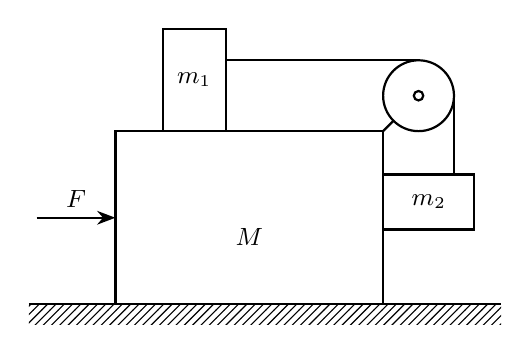
\begin{tikzpicture}[>=Stealth, every node/.style={font=\small}]
  % Ground
  \draw[thick] (-1.1, 0) -- (4.9, 0);
  \fill[pattern=north east lines] (-1.1, -0.25) rectangle (4.9, 0);

  % Block M
  \draw[thick] (0, 0) rectangle (3.4, 2.2);
  \node at (1.7, 0.85) {$M$};

  % Force F
  \draw[->, thick] (-1.0, 1.1) -- node[above] {$F$} (0, 1.1);

  % Block m1
  \draw[thick] (0.6, 2.2) rectangle (1.4, 3.5);
  \node at (1.0, 2.85) {$m_1$};

  % Pulley at top-right of M
  \coordinate (P) at (3.85, 2.65);
  \draw[thick] (3.4, 2.2) -- (P);
  \draw[thick, fill=white] (P) circle (0.45);
  \draw[thick] (P) circle (0.06);

  % Rope
  \draw[thick] (1.4, 3.10) -- (3.85, 3.10);
  \draw[thick] (4.30, 2.65) -- (4.30, 1.65);

  % Block m2
  \draw[thick] (3.4, 0.95) rectangle (4.55, 1.65);
  \node at (3.98, 1.3) {$m_2$};
\end{tikzpicture}
\end{center}
\end{problem}
\clearpage


\begin{problem}{2.1.5}
图 2.5 中小车质量 M、重物质量 m 以及固定斜面的倾角 $\alpha$ 都是已知的，绳子不可伸长，绳子和滑轮的质量以及整个装置中的摩擦力均可略去不计，求小车和重物的加速度.
\begin{center}
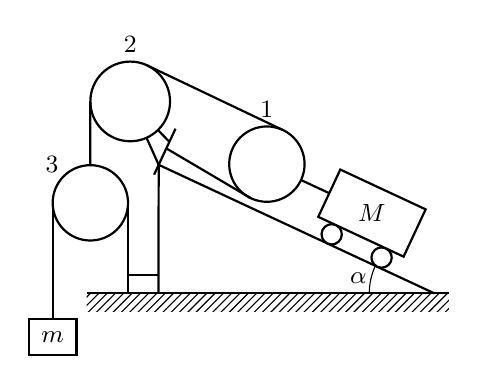
\begin{tikzpicture}[>=Stealth, scale=0.92, every node/.style={font=\small}]
  % Inclined plane angle alpha = 25 deg
  \def\ang{25}
  \coordinate (R) at (5.6, 0);
  \coordinate (T) at ($(R) + (180-\ang:4.2)$); % top of slope (~1.79, 1.775)
  \coordinate (Vbase) at (1.79, 0);

  % Ground
  \draw[thick] (0.8, 0) -- (5.8, 0);
  \fill[pattern=north east lines] (0.8, -0.25) rectangle (5.8, 0);

  % Incline & support stand
  \draw[thick] (R) -- (T) -- (Vbase);
  % Perpendicular stop plate at top of incline
  \coordinate (StopTop) at ($(T) + (90-\ang:0.55)$);
  \coordinate (StopBot) at ($(T) + (-90-\ang:0.15)$);
  \draw[thick] (StopBot) -- (StopTop);

  % Pulley 2 center and mounting bracket
  \coordinate (P2) at (1.40, 2.65);
  \draw[thick] (T) -- (P2) -- ($(T) + (90-\ang:0.35)$);
  \draw[thick, fill=white] (P2) circle (0.55);
  \node at ($(P2) + (90:0.78)$) {$2$};

  % Cart M on incline
  % Along slope from R: distance 1.45 to center of cart
  \coordinate (CartBase) at ($(R) + (180-\ang:1.25)$);
  \begin{scope}[shift={(CartBase)}, rotate=-\ang]
    % Two wheels
    \draw[thick, fill=white] (-0.38, 0.14) circle (0.14);
    \draw[thick, fill=white] (0.38, 0.14) circle (0.14);
    % Cart body
    \draw[thick, fill=white] (-0.65, 0.28) rectangle (0.65, 1.0);
    \node at (0, 0.64) {$M$};
  \end{scope}

  % Pulley 1 (attached to cart M)
  \coordinate (CartFront) at ($(CartBase) + (180-\ang:0.65) + (90-\ang:0.64)$);
  \coordinate (P1) at ($(CartFront) + (180-\ang:0.95)$);
  \draw[thick] (CartFront) -- (P1);
  \draw[thick, fill=white] (P1) circle (0.52);
  \node at ($(P1) + (90:0.75)$) {$1$};

  % Ropes for Pulley 1 and Pulley 2
  % Bottom tangent of P1 to stop plate
  \coordinate (P1bot) at ($(P1) + (-90-\ang:0.52)$);
  \coordinate (StopAnchor) at ($(T) + (90-\ang:0.25)$);
  \draw[thick] (P1bot) -- (StopAnchor);
  % Top tangent of P1 to top-right tangent of P2
  \draw[thick] ($(P1) + (90-\ang:0.52)$) -- ($(P2) + (90-\ang:0.55)$);

  % Pulley 3 (movable pulley)
  \coordinate (P3) at (0.85, 1.25);
  \draw[thick] (0.85, 2.65) -- (P3); % rope from left of P2 to center of P3
  \draw[thick, fill=white] (P3) circle (0.52);
  \node at ($(P3) + (135:0.75)$) {$3$};

  % Rope over Pulley 3: right side anchored to ground, left side to mass m
  \draw[thick] (1.37, 1.25) -- (1.37, 0);
  \draw[thick] (1.37, 0.25) -- (1.79, 0.25); % base brace to stand
  \draw[thick] (0.33, 1.25) -- (0.33, -0.35);

  % Hanging mass m
  \draw[thick] (0.0, -0.85) rectangle (0.66, -0.35);
  \node at (0.33, -0.60) {$m$};

  % Angle alpha
  \draw (4.7, 0) arc (180:180-\ang:0.9);
  \node at (4.55, 0.21) {$\alpha$};
\end{tikzpicture}
\end{center}
\end{problem}
\clearpage


\begin{problem}{2.1.6}
三块质量均为 $m$ 的相同物块叠放在水平面上, 如图 2.6 所示. 各接触面间的摩擦因数均为 $\mu$ , 有一从零不断加大的水平力 $F$ 作用在最下面的物块上. 问 $F$ 达多大时, 最下面的物块才能有对上面两物块的相对运动.
\begin{center}
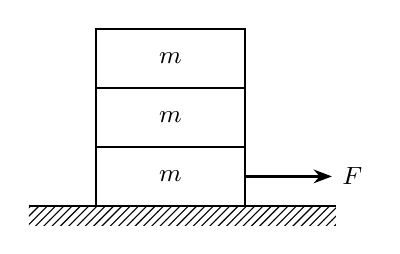
\begin{tikzpicture}[>=Stealth, every node/.style={font=\small}]
  % Ground
  \draw[thick] (-1.8, 0) -- (2.1, 0);
  \fill[pattern=north east lines] (-1.8, -0.25) rectangle (2.1, 0);

  % Three stacked blocks of mass m
  \draw[thick] (-0.95, 0) rectangle (0.95, 0.75);
  \node at (0, 0.375) {$m$};
  \draw[thick] (-0.95, 0.75) rectangle (0.95, 1.5);
  \node at (0, 1.125) {$m$};
  \draw[thick] (-0.95, 1.5) rectangle (0.95, 2.25);
  \node at (0, 1.875) {$m$};

  % Force F on bottom block
  \draw[->, thick] (0.95, 0.375) -- (2.05, 0.375) node[right] {$F$};
\end{tikzpicture}
\end{center}
\end{problem}
\clearpage


\begin{problem}{2.1.7}
质量为 $M$ 的木板静置于水平桌面上(如图2.7所示)，一端 $A$ 与桌边对齐，木板上放着一质量为 $m$ 的小物体，它离板的 $A$ 端距离 $l$ ，桌面长 $L$ .现在板的另一端 $B$ 有一恒定的水平力 $F$ 作用，要将木板从小物体下抽出，又不至于使小物体从桌边落到地上.若各接触面的摩擦因数均为 $\mu ,F$ 至少多大？
\begin{center}
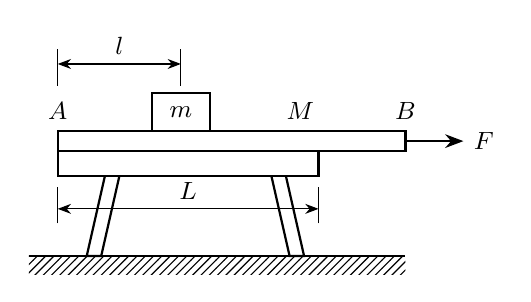
\begin{tikzpicture}[>=Stealth, scale=0.92, every node/.style={font=\small}]
  % Ground
  \draw[thick] (-0.4, 0) -- (4.8, 0);
  \fill[pattern=north east lines] (-0.4, -0.25) rectangle (4.8, 0);

  % Table legs
  \draw[thick] (0.65, 1.1) -- (0.4, 0) -- (0.6, 0) -- (0.85, 1.1);
  \draw[thick] (2.95, 1.1) -- (3.2, 0) -- (3.4, 0) -- (3.15, 1.1);

  % Tabletop (length L = 3.6)
  \draw[thick] (0, 1.1) rectangle (3.6, 1.45);

  % Plank M (from A at x=0 to B at x=4.8)
  \draw[thick] (0, 1.45) rectangle (4.8, 1.72);
  \node[above] at (0, 1.75) {$A$};
  \node[above] at (4.8, 1.75) {$B$};
  \node[above] at (3.35, 1.75) {$M$};

  % Block m on plank (centered at x=1.7)
  \draw[thick] (1.3, 1.72) rectangle (2.1, 2.25);
  \node at (1.7, 1.98) {$m$};

  % Force F
  \draw[->, thick] (4.8, 1.585) -- (5.6, 1.585) node[right] {$F$};

  % Dimension l (from A to center of m)
  \draw (0, 2.35) -- (0, 2.85);
  \draw (1.7, 2.35) -- (1.7, 2.85);
  \draw[<->] (0, 2.65) -- node[above] {$l$} (1.7, 2.65);

  % Dimension L (tabletop length)
  \draw (0, 0.45) -- (0, 0.95);
  \draw (3.6, 0.45) -- (3.6, 0.95);
  \draw[<->] (0, 0.65) -- node[above] {$L$} (3.6, 0.65);
\end{tikzpicture}
\end{center}
\end{problem}
\clearpage


\begin{problem}{2.1.8}
一块砖以初速度 $1.5\mathrm{m / s}$ 在一与水平面成 $30^{\circ}$ 角的斜面上向上运动，摩擦因数 $\mu = \frac{\sqrt{3}}{12}$ . 问经 $0.5\mathrm{s}$ 后，此砖离它的初始位置有多远？
\end{problem}
\clearpage


\begin{problem}{2.1.9}
两个无质量的小环在一个处于铅垂面内的光滑圆环上滑动,一穿过两环的光滑弦线上带有三个重物,两个在两端,一个在两环之间.如果当小环 $A$ 、 $B$ 在离开圆环最高点 $H$ 对环心 $O$ 的张角 $30^{\circ}$ 时处于平衡,如图2.8所示.求系在弦线上的三重物 $D$ 、 $E$ 、 $G$ 的质量之间的关系.
\begin{center}
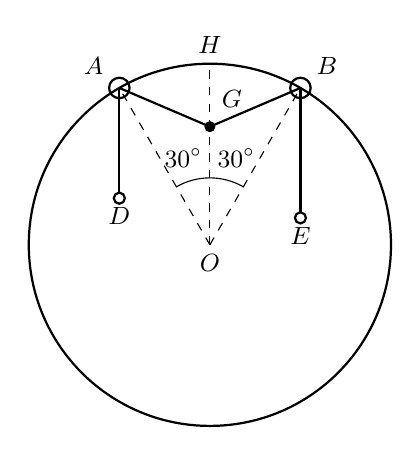
\begin{tikzpicture}[>=Stealth, every node/.style={font=\small}]
  \def\R{2.3}
  \coordinate (O) at (0, 0);
  \coordinate (H) at (0, \R);
  \coordinate (A) at (120:\R);
  \coordinate (B) at (60:\R);
  \coordinate (G) at (0, 1.50);
  \coordinate (D) at ($(A) + (0, -1.4)$);
  \coordinate (E) at ($(B) + (0, -1.65)$);

  % Vertical circular hoop
  \draw[thick] (O) circle (\R);

  % Dashed radii OH, OA, OB
  \draw[dashed] (O) -- (H);
  \draw[dashed] (O) -- (A);
  \draw[dashed] (O) -- (B);

  % Angles 30 deg
  \draw (0, 0.85) arc (90:120:0.85);
  \node at (107:1.15) {$30^\circ$};
  \draw (0, 0.85) arc (90:60:0.85);
  \node at (73:1.15) {$30^\circ$};

  % Small rings A and B
  \draw[thick] (A) circle (0.13);
  \draw[thick] (B) circle (0.13);

  % String A-G-B and vertical ends to D and E
  \draw[thick] (A) -- (G) -- (B);
  \draw[thick] (A) -- (D);
  \draw[thick] (B) -- (E);

  % Weights G, D, E
  \fill (G) circle (2pt);
  \draw[thick, fill=white] (D) circle (2pt);
  \draw[thick, fill=white] (E) circle (2pt);

  % Labels
  \node[above] at (H) {$H$};
  \node[above left] at ($(A)+(-0.08,0.05)$) {$A$};
  \node[above right] at ($(B)+(0.08,0.05)$) {$B$};
  \node at (0.28, 1.85) {$G$};
  \node[below] at (O) {$O$};
  \node[below] at (D) {$D$};
  \node[below] at (E) {$E$};
\end{tikzpicture}
\end{center}
\end{problem}
\clearpage


\begin{problem}{2.1.10}
质量为 $m$ 的小环套在绳上, 绳子跨过定滑轮并在另一端系一质量为 $M$ 的物体. 若绳子不可伸长、不计质量, 绳子与滑轮间的摩擦力可忽略, 小环相对于绳子以加速度 $a$ 下落, 求小环与绳子间的摩擦力.
\begin{center}
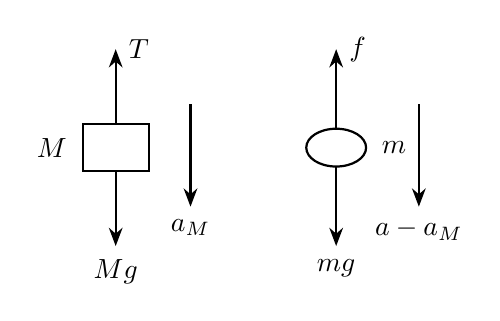
\begin{tikzpicture}[>=Stealth, thick]
  % Left FBD: block M
  \draw (-0.42,-0.30) rectangle (0.42,0.30);
  \node[left=2pt] at (-0.42,0) {$M$};
  \draw[->] (0,0.30) -- (0,1.25) node[right=1pt] {$T$};
  \draw[->] (0,-0.30) -- (0,-1.25) node[below=1pt] {$Mg$};
  \draw[->] (0.95,0.55) -- (0.95,-0.75) node[below=1pt] {$a_M$};

  % Right FBD: ring m
  \draw (2.8,0) ellipse (0.38 and 0.24);
  \node[right=2pt] at (3.18,0) {$m$};
  \draw[->] (2.8,0.24) -- (2.8,1.25) node[right=1pt] {$f$};
  \draw[->] (2.8,-0.24) -- (2.8,-1.25) node[below=1pt] {$mg$};
  \draw[->] (3.85,0.55) -- (3.85,-0.75) node[below=1pt] {$a - a_M$};
\end{tikzpicture}

\end{center}
\end{problem}
\clearpage


\begin{problem}{2.1.11}
一个质量为 $m$ 的物体通过一根质量可以不计的绳子绕水平棒 $1\frac{1}{4}$ 周后于另一端加一水平力 $F$ , 如图2.10所示. 若绳子和棒之间的摩擦因数为 $\mu$ , 要使物体保持静止状态, 应施加多大的水平拉力?
\begin{center}
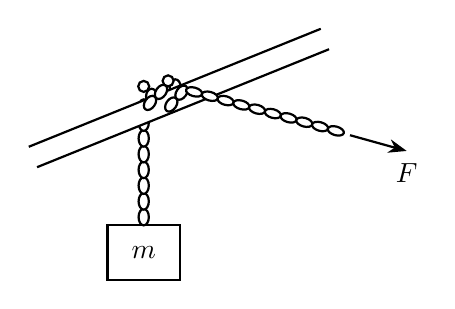
\begin{tikzpicture}[>=Stealth, thick]
  % Hanging block m
  \draw (-1.00,-2.35) rectangle (-0.08,-1.65);
  \node at (-0.54,-2.00) {$m$};

  % Vertical chain links from block up to rod
  \foreach \y in {-1.55,-1.35,-1.15,-0.95,-0.75,-0.55,-0.35,-0.16} {
    \draw[fill=white] (-0.54,\y) ellipse (0.065 and 0.105);
  }

  % Back passes of the chain behind the rod
  \draw[fill=white] (-0.44,-0.02) ellipse (0.07 and 0.10);
  \draw[fill=white] (-0.14,0.10) ellipse (0.07 and 0.10);

  % Tilted horizontal rod
  \begin{scope}[rotate=22]
    \fill[white] (-2.1,-0.14) rectangle (1.9,0.14);
    \draw (-2.1,0.14) -- (1.9,0.14);
    \draw (-2.1,-0.14) -- (1.9,-0.14);
  \end{scope}

  % Front passes wrapping around the rod (1.25 turns)
  \draw[fill=white, rotate around={-35:(-0.46,-0.10)}] (-0.46,-0.10) ellipse (0.065 and 0.10);
  \draw[fill=white, rotate around={-35:(-0.32,0.04)}] (-0.32,0.04) ellipse (0.065 and 0.10);
  \draw[fill=white, rotate around={-35:(-0.19,-0.12)}] (-0.19,-0.12) ellipse (0.065 and 0.10);
  \draw[fill=white, rotate around={-35:(-0.06,0.03)}] (-0.06,0.03) ellipse (0.065 and 0.10);
  \draw[fill=white] (-0.54,0.11) circle (0.07);
  \draw[fill=white] (-0.23,0.18) circle (0.07);

  % Rightward chain and pulling force F
  \foreach \i in {0,...,9} {
    \pgfmathsetmacro{\cx}{0.10 + \i*0.20}
    \pgfmathsetmacro{\cy}{0.04 - \i*0.055}
    \draw[fill=white, rotate around={-15.5:(\cx,\cy)}] (\cx,\cy) ellipse (0.105 and 0.055);
  }
  \draw[->] (2.08,-0.51) -- (2.80,-0.71) node[below=1pt] {$F$};
\end{tikzpicture}

\end{center}
\end{problem}
\clearpage


\begin{problem}{2.1.12}
一根质量为 $M$ 的均质绳子, 两端固定在同一高度的两个钉子上, 在其中点挂一质量为 $m$ 的物体. 设 $\alpha, \beta$ 分别为在绳子中点和端点处绳子的切线方向与竖直方向的夹角, 如图 2.13 所示. 证明:

\[
\frac {\tan \alpha}{\tan \beta} = \frac {M + m}{m}
\]
\begin{center}
\begin{tikzpicture}[>=Stealth, thick]
  % Rope curve from center cusp (0,0) to both nails and tangent extensions
  \draw (0,0) .. controls (-0.85,0.42) and (-1.28,0.95) .. (-1.6,1.8) -- (-1.97,2.78);
  \draw (0,0) .. controls (0.85,0.42) and (1.28,0.95) .. (1.6,1.8) -- (1.97,2.78);

  % Nails
  \fill (-1.6,1.8) circle (2.2pt) node[right=2pt] {钉子};
  \fill (1.6,1.8) circle (2.2pt) node[left=2pt] {钉子};

  % Vertical dashed reference lines and beta angles at nails
  \draw[dashed] (-1.6,1.8) -- (-1.6,2.80);
  \draw[dashed] (1.6,1.8) -- (1.6,2.80);
  \node at (-1.77,2.64) {$\beta$};
  \node at (1.77,2.64) {$\beta$};

  % Vertical dashed reference and tangents at bottom cusp (alpha angles)
  \draw[dashed] (0,0) -- (0,0.85);
  \draw (0,0) -- (-0.95,0.47);
  \draw (0,0) -- (0.95,0.47);
  \node at (-0.28,0.36) {$\alpha$};
  \node at (0.28,0.36) {$\alpha$};

  % Hanging mass m
  \draw (0,0) -- (0,-0.92);
  \draw (-0.52,-0.92) rectangle (0.52,-1.52);
  \node at (0,-1.22) {$m$};
\end{tikzpicture}

\end{center}
\end{problem}
\clearpage


\begin{problem}{2.1.13}
一质量为 $M$ 的均质链条套在一表面光滑、顶角为 $\alpha$ 、底面处于水平的正圆锥上保持静止，若链条平面平行于水平面，求链条中的张力.
\end{problem}
\clearpage


\begin{problem}{2.1.14}
真空中有缺陷的、质量为 950kg 的卫星，被飞船用一根 50m 长、线密度为 1kg/m 的均质绳牵着以 $5m/s^{2}$ 的加速度做匀加速直线运动：

(1) 飞船作用在绳上的力多大?

(2) 计算绳的张力；

(3) 飞船上的人精疲力竭睡着了,飞船助推器的控制电路之一发生短路,使加速度变为 $1 \, m/s^{2}$ 的减速度.这个事故会发生什么后果?
\end{problem}
\clearpage


\begin{problem}{2.1.15}
某人观察到一空间站始终停留在地球同一点的垂直上空. 问观察者位于地球的什么地方? 尽可能详细地描述一下此空间站的轨道.
\end{problem}
\clearpage


\begin{problem}{2.1.16}
公园里有一种转动水平圆盘, 孩子可以坐在盘面上任何地方. 当盘开始加快转速时, 如果摩擦力不够大, 孩子就可能滑出去. 设孩子的质量为 50kg, 摩擦因数为 0.4, 盘的角速度为 2rad/s, 问孩子坐在盘上不被滑开的最大半径多大?
\end{problem}
\clearpage


\begin{problem}{2.1.17}
一小物体放在一半径为 $R$ 的水平圆盘上, 小物体与圆盘间的静摩擦因数为 $\mu$ . 若圆盘绕其轴的角速度逐渐增大到一个值时, 小物体滑出圆盘并最终落到比盘面低 $h$ 的地面上. 问从它离开圆盘的那一点算起, 小物体越过的水平距离多大?
\end{problem}
\clearpage


\begin{problem}{2.1.18}
太阳离银河系中心大约相距 $2.5 \times 10^{4}$ 光年, 近似地以 $1.7 \times 10^{8}$ 年的周期绕此中心做圆周运动. 地球离太阳的距离为 8 光分. 用以上数据, 求出以太阳质量作为单位的银河系的近似质量. 假定作用在太阳上的引力近似为银河系的质量集中在其中心时对太阳的引力.
\end{problem}
\clearpage


\begin{problem}{2.1.19}
用以下近似数据计算地球和太阳的平均密度之比：

$\theta$ 从地球上看太阳的角直径, $\theta=0.5^{\circ}$ ;

l 为地球表面上纬度为 $1^{\circ}$ 的长度, l=100km;

t 为地球公转周期, t=1 年=$3\times 10^{7}$s:

g 为重力加速度, $g=10ms^{-2}$
\end{problem}
\clearpage


\begin{problem}{2.1.20}
(1) 一个均质的球形物体以角速度 $\omega$ 绕对称轴转动, 如果仅仅靠自身的万有引力阻碍球体的离心分解, 该物体必须具有的最小密度多大? 用这一点估计巨蟹座中转速为每秒 30 转的脉冲星的最小密度. (这是公元 1054 年在中国广泛地被观察到的一个超新星爆发的遗迹!)

(2) 如果脉冲星的质量与太阳的质量相当, 约为 $2 \times 10^{30} ~kg$ , 这个脉冲星的最大可能半径多大?

(3) 若脉冲星的密度与核物质的密度相当, 它的半径多大?
\end{problem}
\clearpage


\begin{problem}{2.1.21}
一顶角为 $2\alpha (\alpha > 45^{\circ})$ 的倒立的圆锥面，以恒定角速度 $\omega$ 绕其对称轴旋转，在内表面上距轴为 $r$ 处有一质点，若质点与锥面间的摩擦因数为 $\mu$ ，要使质点相对锥面静止， $\omega$ 应处于什么范围内？
\end{problem}
\clearpage


\begin{problem}{2.1.22}
一圆柱形刚性杆上套一质量为 $m$ 的小环，杆绕通过一端的固定竖直轴以恒定角速度 $\omega$ 旋转，旋转时杆与竖直轴的夹角为 $\alpha$ 。若小环与杆间的摩擦因数为 $\mu$ ，以小环距杆的固定端的距离 $x$ 为坐标列出小环的运动微分方程。
\end{problem}
\clearpage


\begin{problem}{2.1.23}
质量为 m 的小球通过一根原长为 l、劲度系数为 k 的弹性绳系在光滑的水平台面上的 P 点，水平台面绕离 P 点距离为 b 的固定竖直轴以恒定的角速度 $\omega$ 转动。列出小球在弹性绳拉直状态下的运动微分方程。
\end{problem}
\clearpage


\begin{problem}{2.1.24}
质量为 M 的斜劈放在摩擦因数为 $\mu$ 的粗糙水平面上, 质量为 $m_{1}$ 的物体用不计质量、不可伸长的弦线挂起并跨过固连于斜劈的光滑滑轮与在无摩擦的斜劈面上滑动的质量为 $m_{2}$ 的物体相连, 斜劈面的倾角为 $\theta$ . 如图 2.17 所示.

(1) 求当 $\mu$ 非常大时 $m_{1}$ 和 $m_{2}$ 的加速度以及弦线的张力；

(2) 求使斜劈能保持静止的最小摩擦因数；

(3) 若 $\mu$ 不够大, 斜劈不能保持静止, 有向左的加速度 $a_{M}$ , 求此 $a_{M}$ , 列出足够的方程即可, 不必解出 $a_{M}$ . 设滑轮很小, $m_{1}, M$ 紧靠时, 连结 $m_{1}$ 的弦线仍可视为在竖直方向.
\begin{center}
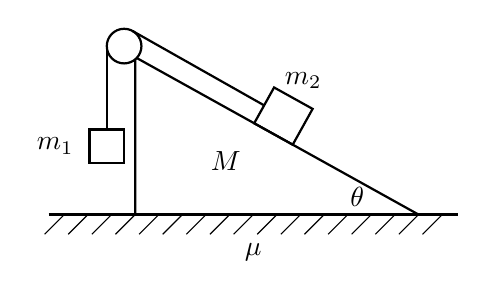
\begin{tikzpicture}[>=Stealth, thick]
  % Rough horizontal ground
  \draw (-1.1,0) -- (4.1,0);
  \foreach \x in {-0.9,-0.6,...,3.9} {
    \draw[thin] (\x,0) -- (\x-0.25,-0.25);
  }
  \node at (1.5,-0.48) {$\mu$};

  % Wedge M
  \draw (0,0) -- (3.6,0) -- (0,2.0) -- cycle;
  \node at (1.15,0.68) {$M$};
  \node at (2.82,0.22) {$\theta$};

  % Pulley at top-left corner
  \draw (0,2.0) -- (-0.14,2.14);
  \draw[fill=white] (-0.14,2.14) circle (0.22);

  % Hanging mass m1
  \draw (-0.36,2.14) -- (-0.36,1.08);
  \draw (-0.58,0.66) rectangle (-0.14,1.08);
  \node[left=2pt] at (-0.58,0.87) {$m_1$};

  % Block m2 on the incline and string
  \begin{scope}[shift={(1.512,1.16)}, rotate=-29.05]
    \draw (0,0) rectangle (0.56,0.52);
    \node at (0.28,0.78) {$m_2$};
    \coordinate (m2attach) at (0,0.26);
  \end{scope}
  \draw (-0.033,2.332) -- (m2attach);
\end{tikzpicture}

\end{center}
\end{problem}
\clearpage


\begin{problem}{2.1.25}
一质量为 M 的、上表面水平的楔形物体，在倾角为 $\alpha$ 的固定的光滑斜面上运动，楔形物体上放一质量为 m 的质点，如图 2.20 所示。若 m、M 间无摩擦，求：

(1) $m$ 相对于 $M$ 的加速度；

(2) $M$ 对斜面的压力.
\begin{center}
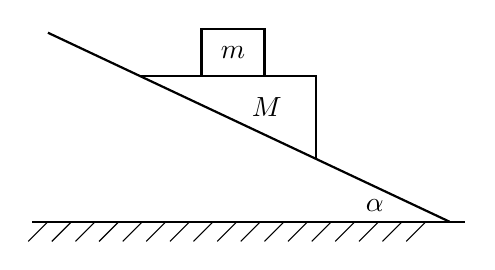
\begin{tikzpicture}[>=Stealth, thick]
  % Horizontal ground
  \draw (-1.0,0) -- (4.5,0);
  \foreach \x in {-0.8,-0.5,...,4.3} {
    \draw[thin] (\x,0) -- (\x-0.25,-0.25);
  }

  % Fixed inclined plane
  \draw (-0.8,2.4) -- (4.3,0);
  \node at (3.35,0.20) {$\alpha$};

  % Wedge M with horizontal top surface
  \draw (0.369,1.85) -- (2.6,1.85) -- (2.6,0.80);
  \node at (1.98,1.45) {$M$};

  % Block m on top of wedge M
  \draw (1.15,1.85) rectangle (1.95,2.45);
  \node at (1.55,2.15) {$m$};
\end{tikzpicture}

\end{center}
\end{problem}
\clearpage


\begin{problem}{2.1.26}
图 2.22 中水平桌面上的滑块质量为 M，一条其两端分别系着质量为 $m_{1}$ 、 $m_{2}$ 

的两个物体的不计质量、不可伸长的细绳套在滑块上，滑块、绳子与桌面相互间均无摩擦。试证明滑块的加速度为

\[
a = \frac {4 m _ {1} m _ {2}}{M (m _ {1} + m _ {2}) + 4 m _ {1} m _ {2}} g
\]
\begin{center}
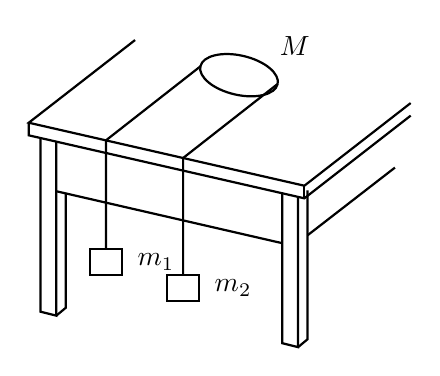
\begin{tikzpicture}[>=Stealth, thick]
  % Table legs and apron (drawn first so hanging strings pass cleanly in front)
  \draw (-2.05,0.16) -- (-2.05,-2.05) -- (-1.85,-2.10) -- (-1.85,0.11);
  \draw (-1.85,-2.10) -- (-1.73,-2.00) -- (-1.73,-0.55);
  \draw (1.02,-0.546) -- (1.02,-2.45) -- (1.22,-2.50) -- (1.22,-0.592);
  \draw (1.22,-2.50) -- (1.34,-2.40) -- (1.34,-0.51);

  % Apron under tabletop
  \draw (-1.85,-0.52) -- (1.02,-1.18);
  \draw (1.34,-1.08) -- (2.45,-0.22);

  % Tabletop surface and front/side thickness
  \draw (-0.85,1.40) -- (-2.20,0.35) -- (1.30,-0.45) -- (2.65,0.60);
  \draw (-2.20,0.35) -- (-2.20,0.19) -- (1.30,-0.61) -- (2.65,0.44);
  \draw (1.30,-0.45) -- (1.30,-0.61);

  % Slider M (ellipse on tabletop) and string wrapped around it
  \draw[rotate around={-13:(0.47,0.954)}] (0.47,0.954) ellipse (0.503 and 0.25);
  \node at (1.18,1.32) {$M$};
  \draw (-0.02,1.066) -- (-1.22,0.126) -- (-1.22,-1.25);
  \draw (0.96,0.842) -- (-0.24,-0.098) -- (-0.24,-1.58);

  % Hanging masses m1 and m2
  \draw[fill=white] (-1.42,-1.25) rectangle (-1.02,-1.58);
  \node[right=2pt] at (-1.02,-1.42) {$m_1$};
  \draw[fill=white] (-0.44,-1.58) rectangle (-0.04,-1.91);
  \node[right=2pt] at (-0.04,-1.75) {$m_2$};
\end{tikzpicture}

\end{center}
\end{problem}
\clearpage


\begin{problem}{2.1.27}
$q_{1}, q_{2}$ 轴在竖直的 $xy$ 平面内，与 $x$ 轴的夹角分别为 $\alpha$ 和 $\beta$ . 一个抛射体在 $xy$ 平面内运动，今取 $q_{1}, q_{2}$ 为坐标，给出或导出抛射体的运动微分方程. 重力沿 $y$ 轴的负方向.
\end{problem}
\clearpage


\begin{problem}{2.1.28}
质量分别为 $M$ 和 $M + m$ 的两个人, 分别拉住跨过定滑轮两边的绳子往上爬. 开始时两人与滑轮的距离都是 $h$ , 都从静止开始爬. 设绳子不可伸长, 绳子质量与绳子、滑轮间的摩擦力均可不计. 证明: 如质量较轻的人在 $t$ 秒内爬到滑轮, 这时质量较重的人与滑轮的距离为 $\frac{m}{M + m}\left(h + \frac{1}{2} gt^2\right)$ .
\end{problem}
\clearpage


\begin{problem}{2.1.29}
一质量为 m 的跳水运动员, 初速为零地从 10m 跳台上跳下.

(1) 求入水速度和从起跳到入水大致所用的时间；

(2) 假定作用在跳水者身上水的浮力和他所受的重力正好抵消, 作用在他身上的水的黏滞力大小为 $bv^2$ , 试列出跳水员在水中垂直下沉的运动微分方程, 以边界条件 $x = 0$ 处 $v = v_0$ , 求解速度 $v$ 作为水面下深度 $x$ 的函数;

(3) 若 $\frac{b}{m}=0.4m^{-1}$ ，求当 $v=\frac{1}{10}v$ 时的深度；

(4) 求解跳水员在水下的垂直深度作为在水下的时间的函数.
\end{problem}
\clearpage


\begin{problem}{2.1.30}
一个质量为 $m$ 的质点以初速 $v$ 在 $y$ 方向投射到沿 $x$ 方向以不变速度 $V$ 运动着的水平皮带上并留在上面运动. 若质点与皮带间的滑动摩擦因数为 $\mu$ , 质点接触皮带的初位置取为固定的 $xy$ 坐标系的原点, 求质点在皮带上刚停止滑动时的 $xy$ 坐标.
\end{problem}
\clearpage


\begin{problem}{2.1.31}
在水平的 $xy$ 平面内有一留声机转盘, 它以恒定的角速度 $\omega$ 绕过盘心的铅垂轴旋转. 在转盘上滑动的物体在水平方向受到两个真实力作用: 一个是大小为 $kr(r$ 为质点至盘心的距离, $k$ 为常量), 方向指向盘心的弹性力; 另一个是摩擦力, 与相对速度成正比, 比例系数为 $c, c$ 是正值常量, 物体可视为质点.

(1) 如物体待在盘上任何位置均能相对转盘保持静止, 问 k 有多大?

(2) 假设 k 是(1)问所得之值, 在一般的初始条件下, 求物体的相对速度 $\dot{x}$ 、 $\dot{y}$ ;

(3) 用(2)的结果进而求 $x(t)$ 和 $y(t)$ .
\end{problem}
\clearpage


\begin{problem}{2.1.32}
一个质点垂直上抛, 初速为 $v_{0}$ , 如空气阻力与速率的平方成正比, 证明: 回到初始位置时的速率为 $\frac{v_{0} v_{t}}{(v_{0}^{2} + v_{t}^{2})^{1/2}}$ , 其中 $v_{t}$ 是极限速率.
\end{problem}
\clearpage


\begin{problem}{2.1.33}
两个质量均为 $m$ 的质点 $A$ 和 $B$ 连在一个劲度系数为 $k$ 的弹簧的两端. 开始两质点静放在光滑的水平面上, 弹簧处于原长, 然后沿 $AB$ 方向给 $B$ 以恒力 $ka$ . 求两质点的运动学方程.
\end{problem}
\clearpage


\begin{problem}{2.1.34}
质量为 $m$ 的质点在阻力等于 $mk(v^3 + a^2 v)$ 的介质中运动, 其中 $k$ 和 $a$ 均为常量, 初速度为 $v_0$ . 求其路程与时间的关系, 并由此导出 $k \to 0$ 时的关系来检验所得结果的正确性.
\end{problem}
\clearpage


\begin{problem}{2.1.35}
质量为 $m$ 的质点静止地连在一弹簧的端点，弹簧的劲度系数为 $k$ ，并悬挂在固定支点上。当 $t = 0$ 时，对质点施一向下的恒力 $F$ ，作用时间为 $t_0$ 。证明：当外力去掉后，质点由其平衡位置 $x = x_0$ 所做的位移为

\[
x - x _ {0} = \frac {F}{k} [ \cos \omega (t - t _ {0}) - \cos \omega t ]
\]

其中 $\omega^{2}=\frac{k}{m}.$
\end{problem}
\clearpage


\begin{problem}{2.1.36}
空间内有均匀的电场和磁场, $E=Ei,B=B(\cos\alpha i+\sin\alpha j)$ ,$\alpha$为常量.具有质量为m、电量为q的粒子在坐标系原点以初速 $v_{0}=\dot{x}_{0}i+\dot{y}_{0}j+\dot{z}_{0}k$ 开始运动.若重力可忽略不计,求质点以后的运动.
\end{problem}
\clearpage


\begin{problem}{2.1.37}
具有质量 m 和电量 q 的质点, 以速度 $V_{0}$ 垂直于电场方向进入按 E = $E_{0}\cos\omega t$ 规律变化的均匀电场, 若质点还受到一个跟速度一次幂成比例的阻力 R = -$\gamma$v, $\gamma$ 为正值常量. 求质点的运动(不计重力的作用).
\end{problem}
\clearpage


\begin{problem}{2.1.38}
一长度为 L 的水平封闭圆管绕其一端的竖直轴以恒定的角速度 $\omega$ 旋转，管内装有密度为 $\rho_{0}$ 的液体及一截面半径略小于管内径的长为 l、密度为 $\rho(\rho > \rho_{0})$ 的小圆柱体。开始时，小圆柱体紧靠轴并相对于圆管静止。问经多长时间小圆柱体到达管的另一端。
\end{problem}
\clearpage


\begin{problem}{2.1.39}
一个质点以初始速率 $v_{0}$ 、仰角 $\alpha$ 抛出，若空气阻力与速率的平方成正比，比例系数为 $mk, m$ 为质点的质量。证明：

(1) 运动微分方程可以写成

\[
\ddot {x} = - k \dot {x} \dot {s}, \quad \ddot {y} = - k \dot {y} \dot {s} - g
\]

其中 x 轴沿水平方向，y 轴竖直向上， $\dot{s}^{2}=\dot{x}^{2}+\dot{y}^{2}$ ;

(2) 轨道微分方程可写为

\[
\frac {\mathrm{d} ^ {2} y}{\mathrm{d} x ^ {2}} = - g \mathrm{e} ^ {2 k s} / (v _ {0} \cos \alpha) ^ {2}
\]

其中 s 是自抛射点沿轨道经过的路程；

(3) 忽略空气阻力时,积分上述轨道微分方程,可得抛物线形式的轨道.
\end{problem}
\clearpage


\begin{problem}{2.1.40}
有一光滑旋转抛物面,其方程为

\[
z = - \frac {1}{2} (x ^ {2} + y ^ {2})
\]

z 轴竖直向上. 在其顶点有一质量为 m 的小物体, 受到微小扰动后自静止开始下滑. 求抛

物面对物体的作用力(取质点运动平面为 $xz$ 平面.)
\end{problem}
\clearpage


\begin{problem}{2.1.41}
一个 $3:4:5$ 的斜面固连在一转盘上, 如图 2.28 所示, 一木块静止在斜面上, 斜面和木块之间的静摩擦因数 $\mu_{s} = \frac{1}{4}$ . 求此木块能保持在离转盘中心的水平距离为 $40\mathrm{cm}$ 处相对转盘不动的最小转动角速度 $\omega$ .
\begin{center}
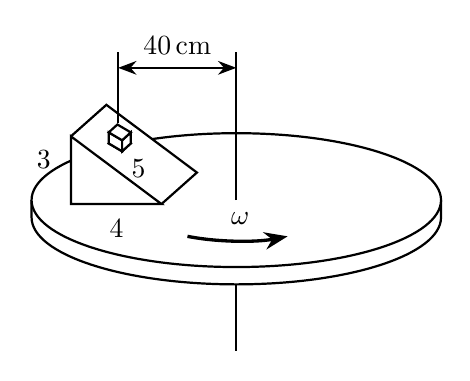
\begin{tikzpicture}[>=Stealth, thick]
  % Lower shaft
  \draw (0,-1.07) -- (0,-1.92);

  % Turntable disk (3D ellipse + rim)
  \draw (-2.6,0) -- (-2.6,-0.22) arc (180:360:2.6 and 0.85) -- (2.6,0);
  \draw[fill=white] (0,0) ellipse (2.6 and 0.85);

  % Central upper shaft
  \draw (0,0) -- (0,1.88);

  % Rotation arrow omega
  \draw[->, very thick] (-0.62,-0.46) arc (238:302:1.2 and 0.38);
  \node at (0.05,-0.24) {$\omega$};

  % 3:4:5 wedge on turntable
  \coordinate (W1) at (-2.10,-0.05);
  \coordinate (W2) at (-0.95,-0.05);
  \coordinate (W3) at (-2.10,0.81);
  \coordinate (W2b) at (-0.50,0.35);
  \coordinate (W3b) at (-1.65,1.21);

  \fill[white] (W1) -- (W2) -- (W2b) -- (W3b) -- (W3) -- cycle;
  \draw (W1) -- (W2) -- (W3) -- cycle;
  \draw (W3) -- (W3b) -- (W2b) -- (W2);

  \node[left=3pt] at (-2.12,0.52) {$3$};
  \node[below=2pt] at (-1.52,-0.05) {$4$};
  \node at (-1.24,0.40) {$5$};

  % Small block resting on the sloped face
  \filldraw[fill=white] (-1.62,0.72) -- (-1.45,0.62) -- (-1.34,0.72) -- (-1.51,0.82) -- cycle;
  \filldraw[fill=white] (-1.62,0.72) -- (-1.62,0.86) -- (-1.45,0.76) -- (-1.45,0.62) -- cycle;
  \filldraw[fill=white] (-1.45,0.62) -- (-1.45,0.76) -- (-1.34,0.86) -- (-1.34,0.72) -- cycle;
  \filldraw[fill=white] (-1.62,0.86) -- (-1.45,0.76) -- (-1.34,0.86) -- (-1.51,0.96) -- cycle;

  % 40 cm horizontal distance indicator
  \draw (-1.50,0.98) -- (-1.50,1.88);
  \draw[<->] (-1.50,1.68) -- (0,1.68) node[midway, above=1pt] {$40\,\mathrm{cm}$};
\end{tikzpicture}

\end{center}
\end{problem}
\clearpage


\begin{problem}{2.1.42}
一水平转盘由静止开始启动，并以匀角加速度 $0.04\pi \mathrm{rad} / \mathrm{s}^2$ 加速。一小孩坐在离转盘 $6\mathrm{m}$ 远的椅子上，手中握着一个 $2\mathrm{kg}$ 的球。求转盘启动5s后那一瞬间，小孩为握住球必须施以的力的大小和方向。
\end{problem}
\clearpage


\begin{problem}{2.1.43}
一个在竖直平面内半径为 $a$ 的圆环，以角速度 $\omega$ 绕其竖直直径旋转。一质量为 $m$ 的小球在环上无摩擦地滑动，如图2.30所示。

(1) 在什么特殊条件下, 小球在 $\theta=0$ 处是稳定平衡?

(2) 当 $\omega$ 为何值时, 小球可处于另一稳定平衡位置, 求出这时的 $\theta$ 值.
\begin{center}
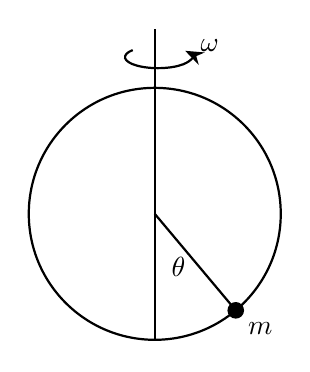
\begin{tikzpicture}[>=Stealth, thick]
  % Circular hoop
  \draw (0,0) circle (1.6);

  % Vertical rotation axis
  \draw (0,-1.6) -- (0,2.35);

  % Rotation arrow omega
  \draw[->] (-0.28,2.08) arc (140:395:0.42 and 0.14);
  \node[right=2pt] at (0.38,2.14) {$\omega$};

  % Radius to bead m at angle theta = 40 deg from downward vertical
  \draw (0,0) -- (-50:1.6);
  \fill (-50:1.6) circle (3pt) node[below right=1pt] {$m$};
  \node at (0.30,-0.68) {$\theta$};
\end{tikzpicture}

\end{center}
\end{problem}
\clearpage


\begin{problem}{2.1.44}
一光滑的水平圆盘以角速度 $\omega$ 绕通过盘心的垂直轴转动. 在圆盘上位于离盘心距离 $R$ 的人给质量为 $m$ 的光滑硬币（忽略大小）朝向盘心方向的推力，使硬币得到相对于圆盘的初速度 $v$ . 证明：在圆盘上的人看来，在一段时间内 $[( \omega t)^2$ 可以忽略]运动是一条抛物线，给出这条抛物线的方程.
\end{problem}
\clearpage


\begin{problem}{2.1.45}
卫星绕地球做圆轨道运动,卫星内的宇航员将一个小物体放在卫星质心和地心连线上离卫星质心 $\Delta r$ 处然后释放.求在卫星参考系中宇航员所看到的释放后物体的运动(设卫星像月球那样朝向地球的部分始终朝向地球).
\end{problem}
\clearpage


\begin{problem}{2.1.46}
一质量为 $m$ 的质点用原长为 $l$ 、劲度系数为 $k$ 的弹簧挂起来， $t = 0$ 时，弹簧上端的支撑点开始上下按正弦函数做振动，振动的振幅为 $A$ ，角频率为 $\omega (\omega \neq \sqrt{k / m})$ 。求质点的运动。
\end{problem}
\clearpage


\begin{problem}{2.1.47}
一块光滑的水平板绕过板上一点的竖直轴做恒定角速度为 $\omega$ 的转动. 一质点用一根原长为零、劲度系数为 $k$ 的弹簧连接于轴与平板的交点. 若取开始时质点与交点 (取为坐标系原点) 的连线为 $x$ 轴, $z$ 轴沿 $\omega$ 的方向, 质点开始在 $(a,0)$ 处以 $(0,v_0)$ 的速度运动, 求质点的运动学方程 $x(t), y(t)$ .
\end{problem}
\clearpage


\begin{problem}{2.1.48}
考虑一组荷质比 e/m 都相同的带电粒子, 证明: 这些粒子在一个小的磁场 B (常矢量) 中的运动同在一个适当选择的角速度 $\omega$ 转动的参考系中看到的没有这个磁场的运动相同, 求这相应的 $\omega$ 值, 并对“小场”作出说明.
\end{problem}
\clearpage


\begin{problem}{2.1.49}
一个质量为 $m$ 的质点在光滑的水平面上以角速度 $\omega$ 做匀速率圆周运动, 其向心力是通过一劲度系数为 $k$ 的弹簧提供的. 使质点突然获得一个很小的径向速度分量, 求所引起的径向振动的频率.
\end{problem}
\clearpage


\begin{problem}{2.1.50}
一个质量为 $M$ 的小珠套在光滑的水平的金属丝上, 另一个质量为 $m$ 的质点通过无质量的不可伸长的、长度为 $a$ 的绳子连在小珠上. 握住小珠与质点, 使绳子沿金属丝拉直, 然后突然释放. 求此后绳子张力与绳子、竖直线间夹角 $\theta$ 的关系.
\end{problem}
\clearpage


\begin{problem}{2.1.51}
质量分别为 $m$ 和 $M$ 的两个小环可在一光滑的竖直平面内的圆圈上运动，两环被一根无质量的、不可伸长的绳子连着。证明：只要绳子保持拉紧，绳子张力为 $2mMg\tan \alpha \cos \theta /(m + M)$ ，其中 $2\alpha$ 是绳子拉紧时对圈心所张的角， $\theta$ 是绳子与水平线间的夹角， $g$ 为重力加速度。
\end{problem}
\clearpage


\begin{problem}{2.1.52}
三个点源等距离地固定在一个半径为 $a$ 、圆心为原点的圆周上，每个点源对质量为 $m$ 的质点的作用力为引力 $F = -kR$ ，其中 $k$ 为正值常量， $R$ 为质点对点源的位矢。质点在 $t = 0$ 时放入力场，初始条件为 $r = r_0 \cdot r = v_0$ ，如图2.34所示。

(1) 求解质点的运动, 用 $r_0, v_0$ 及其他参数表示 $\boldsymbol{r}(t)$ ;

(2) 在什么条件下, 质点的运动轨道为圆?
\begin{center}
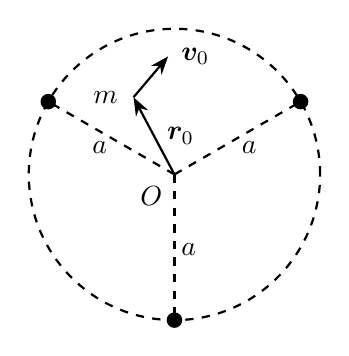
\begin{tikzpicture}[>=Stealth, thick]
  % Dashed circle of radius a
  \draw[dashed] (0,0) circle (1.85);
  \node[below left=1pt] at (0,0) {$O$};

  % Three equally spaced point sources and dashed radii
  \foreach \ang in {30,150,-90} {
    \draw[dashed] (0,0) -- (\ang:1.85);
    \fill (\ang:1.85) circle (2.8pt);
  }
  \node at (-0.95,0.34) {$a$};
  \node at (0.95,0.34) {$a$};
  \node at (0.18,-0.95) {$a$};

  % Particle m, position vector r0, and initial velocity v0
  \coordinate (M) at (-0.52,0.98);
  \draw[->] (0,0) -- (M) node[midway, right=1pt] {$\boldsymbol{r}_0$};
  \node[left=2pt] at (M) {$m$};
  \draw[->] (M) -- (-0.08,1.50) node[right=1pt] {$\boldsymbol{v}_0$};
\end{tikzpicture}

\end{center}
\end{problem}
\clearpage


\begin{problem}{2.1.53}
$n$ 个质点质量均为 $m$ , 任何两个质点间相互作用力为斥力, 大小与它们间的距离成正比, 比例系数为 $\mu m^2$ . 开始把它们静止地放在一个光滑的水平面上处于以 $O$ 为中心、 $a$ 为半径的圆圈上的对称位置. 证明: 同时释放后, 任一质点位于离 $O$ 点距离 $r$ 处时的速率为

$\left[\mu nm(r^2 - a^2)\right]^{1/2}$ 提示： $2\left[\sin^2 \frac{\pi}{n} + \sin^2 \frac{2\pi}{n} + \cdots + \sin^2 \frac{(n-1)\pi}{n}\right] = n$ （ $n \geqslant 2$ ).
\end{problem}
\clearpage


\begin{problem}{2.1.54}
考虑一质量为 $m$ 的粒子在力 $\bm{F} = -kr$ 作用下运动，这里 $k$ 是正值常量， $\bm{r}$ 是粒子的位矢.

(1) 证明粒子在一平面内运动；

(2) 设在 $t = 0$ 时, $x = a, y = 0, \dot{x} = 0, \dot{y} = v_0$ , 求 $x(t)$ 和 $y(t)$ ;

(3) 证明该轨道是一椭圆；

(4) 求出周期.
\end{problem}
\clearpage


\begin{problem}{2.1.55}
质量分别为 $m$ 及 $m'$ 的两个质点，用未伸缩时长度为 $a$ 的弹性绳相连，绳的劲度系数 $k = \frac{2mm' \omega^2}{m + m'}$ . 将此系统放在光滑的水平管内，管子绕通过管上某点的竖直轴以恒定角速度 $\omega$ 转动. 开始时，两质点相对于管子是静止的，两质点间距为 $a$ . 试求此后任何时刻两质点间的距离.
\end{problem}
\clearpage


\begin{problem}{2.1.56}
质量为 $m$ 的小环套在半径为 $a$ 的光滑圆圈上，可在其上滑动。如圆圈在水平面内以恒定角速度 $\omega$ 绕圈上某点 $O$ 转动，转轴垂直于水平面。试求小环沿圆圈切线方向的运动微分方程。
\end{problem}
\clearpage


\begin{problem}{2.1.57}
两个粒子质量为 $m$ 、带正电荷 $q$ ，用劲度系数为 $k$ 、平衡长度为零的弹簧相连。沿水平方向有恒定电场 $E = E_0 i$ ，考虑粒子之间的库仑力，忽略磁效应、辐射效应和相对论效应等，假定粒子没有碰撞。

(1) 如果粒子在水平 x 方向的光滑直线上滑动, 它们之间的距离 d 不变. 求 d;

(2) 若(1)中两粒子间的距离 $d(t)$ 为在一个平衡位置附近的小振动, 求频率;

(3) 若粒子在水平的光滑桌面上滑动, 求运动微分方程的通解, 可在答案中保留积分.
\end{problem}
\clearpage


\begin{problem}{2.1.58}
一个半径为 $R$ 的半球形碗以不变角速度 $\Omega$ 绕竖直的对称轴转动. 质量为 $M$ 的一个粒子在重力影响下在碗的内表面运动, 粒子除受到碗面的支持力外, 还受到一个摩擦力 $F = -kv$ , 其中 $k$ 为正值常量, $v$ 是相对于碗的速度.

（1）用球坐标 $\theta, \varphi$ （坐标原点取在碗心），写出粒子相对于转动参考系的运动微分方程. 证明：如果 $\Omega > \sqrt{\frac{g}{R}}$ ，除了碗底这个平衡位置以外，存在第二个平衡位置，并求出这第二个平衡位置的 $\theta$ 值.

(2) 考虑粒子在碗底这个平衡位置附近的运动。在此平衡点取一个固定的笛卡儿坐标系 $x, y, z$ ，除计算重力提供的恢复力以外，不考虑碗的曲率。证明：对于 $|x| \ll R$ 、 $|y| \ll R$ ，粒子的一个特解为

\[
x = \operatorname{Re} (x _ {0} \mathrm{e} ^ {\lambda t}), \quad y = \operatorname{Re} (y _ {0} \mathrm{e} ^ {\lambda t})
\]

其中 $\lambda$ 满足

\[
\left(\lambda^ {2} + \frac {k}{M} \lambda + \frac {g}{R}\right) ^ {2} + \left(\frac {k}{M}\right) ^ {2} \Omega^ {2} = 0
\]

(3) 求碗的角速度 $\Omega_{0}$ ，对于此角速度，粒子的运动是周期性的.
\end{problem}
\clearpage


\begin{problem}{2.1.59}
一个质点在重力作用下沿一粗糙的竖直的圆周运动. 如从水平直径的一端的静止状态开始运动, 到圆的最低点时刚好静止. 求摩擦因数 $\mu$ 必须满足的关系.
\end{problem}
\clearpage


\begin{problem}{2.1.60}
一个质量为 $M$ 的小球, 用一根劲度系数为 $k$ 、自然长度为零的无质量弹簧悬挂于天花板下, 小球下面挂一根相同的弹簧, 原处于平衡状态. 今有一个力 $F(t)$ 作用于下面弹簧的下端, 如图 2.42 所示. 求上面弹簧的长度 $x_{1}$ 与 $F(t)$ 的关系; 如 $F(t) = \lambda t$ , $\lambda$ 为常量, 求 $x_{1}(t)$ .
\begin{center}
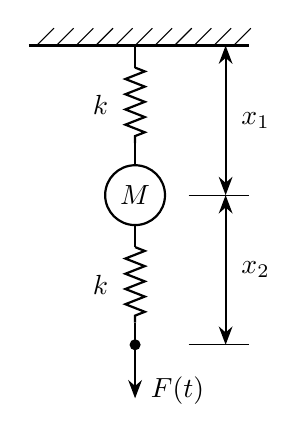
\begin{tikzpicture}[>=Stealth, thick]
  % Ceiling with hatching
  \draw (-1.35,0) -- (1.45,0);
  \foreach \x in {-1.25,-1.00,...,1.25} {
    \draw[thin] (\x,0) -- (\x+0.22,0.22);
  }

  % Upper spring k
  \draw (0,0) -- (0,-0.28);
  \draw[decorate, decoration={zigzag, segment length=5.5pt, amplitude=3.5pt}] (0,-0.28) -- (0,-1.24);
  \node[left=6pt] at (0,-0.76) {$k$};
  \draw (0,-1.24) -- (0,-1.52);

  % Ball M
  \draw (0,-1.90) circle (0.38);
  \node at (0,-1.90) {$M$};

  % Lower spring k
  \draw (0,-2.28) -- (0,-2.56);
  \draw[decorate, decoration={zigzag, segment length=5.5pt, amplitude=3.5pt}] (0,-2.56) -- (0,-3.52);
  \node[left=6pt] at (0,-3.04) {$k$};
  \draw (0,-3.52) -- (0,-3.80);

  % Bottom point and applied force F(t)
  \fill (0,-3.80) circle (2pt);
  \draw[->] (0,-3.80) -- (0,-4.48) node[pos=0.85, right=2pt] {$F(t)$};

  % Dimension ticks and arrows x1, x2
  \draw[thin] (0.68,-1.90) -- (1.45,-1.90);
  \draw[thin] (0.68,-3.80) -- (1.45,-3.80);
  \draw[<->] (1.15,0) -- (1.15,-1.90) node[midway, right=2pt] {$x_1$};
  \draw[<->] (1.15,-1.90) -- (1.15,-3.80) node[midway, right=2pt] {$x_2$};
\end{tikzpicture}

\end{center}
\end{problem}
\clearpage


\begin{problem}{2.1.61}
单位质量的质点在阻力与速度成正比的介质中运动, 比例系数为 $\beta$ , 在一个按指数衰减的力 $F_{0}e^{-\gamma t}$ (其中 $F_{0}, \gamma$ 均为常量) 作用下自静止开始运动. 用拉普拉斯变换法求解该质点此后的运动规律.
\end{problem}
\clearpage


\begin{problem}{2.1.62}
用积分因子法求解上题.
\end{problem}
\clearpage


\begin{problem}{2.1.63}
质量为 $m$ 的质点在图2.43所示的力作用下做直线运动.

(1) 求 $F(t)$ 的拉普拉斯变换的象函数 $f(p)$ ;

(2) 用拉普拉斯变换法求此运动的通解；

(3) 直接用逐次积分的方法求通解.

提示： $\frac{1}{p^{\mu}}\mathrm{e}^{-kp}(\mu >0)$ 的原函数为

\[
\frac {(t - k) ^ {\mu - 1}}{\Gamma (\mu)} u (t - k)
\]

其中

\[
\begin{array}{l} u (t - k) = \left\{ \begin{array}{l l} 0 & t <   k \\ 1 & t \geqslant k \end{array} \right. \\ \Gamma (\mu) = (\mu - 1)! \end{array}
\]
\begin{center}
\begin{tikzpicture}[>=Stealth, font=\small]
  \draw[->] (0,0) -- (4.8,0) node[below left=2pt and 0pt] {$t$};
  \draw[->] (0,0) -- (0,2.8) node[left=2pt] {$F$};
  \node[below left=1pt] at (0,0) {$O$};

  \draw[thick] (0,0) -- (1.4,2.0) -- (3.2,2.0);
  \draw[dashed] (0,2.0) node[left=2pt] {$F_0$} -- (1.4,2.0);
  \draw[dashed] (1.4,2.0) -- (1.4,0) node[below=2pt] {$t_1$};
  \draw[dashed] (3.2,2.0) -- (3.2,0) node[below=2pt] {$t_2$};
\end{tikzpicture}

\end{center}
\end{problem}
\clearpage


\begin{problem}{2.1.64}
质量为 m 的质点在恢复力 -kx 和阻力 $-\gamma \dot{x}$ 以及周期性驱动力(每个周期)

\[
F (t) = \left\{ \begin{array}{l l} A \sin \omega t & 0 <   t \leqslant \frac {\pi}{\omega} \\ 0 & \frac {\pi}{\omega} <   t \leqslant \frac {2 \pi}{\omega} \end{array} \right.
\]

的共同作用下做受迫振动. 用傅里叶级数求解稳态时的运动学方程(要求写出级数的前四项).
\end{problem}
\clearpage


\begin{problem}{2.1.65}
考虑一阻尼振子,其运动微分方程为

\[
\ddot {x} + \lambda \dot {x} | \dot {x} | + \omega_ {0} ^ {2} x = 0
\]

$\lambda$ 为小的正值常量, 初始条件为 $x(0) = a, \dot{x}(0) = 0$ . 用微扰法证明第一个后半周位移与前半周位移之比 (精确到 $\lambda$ 的一次方) 为 $1 - \frac{4}{3} \lambda a$ .
\end{problem}
\clearpage


\begin{problem}{2.1.66}
一物体在北纬 $40^{\circ}$ 的地球表面上方高 $h$ 处从静止降落, 若 $h = 100\mathrm{m}$ , 计算由于科里奥利力引起的着地点的横向位移.
\end{problem}
\clearpage


\begin{problem}{2.1.67}
由于地球的自转而引起的下列偏离的大小和方向是什么？

（1）从北纬 $\theta^{\circ}$ 、高 $L$ 的塔顶到底部悬挂的铅垂线下的摆锤；

(2) 从顶部降落的物体的着地点.
\end{problem}
\clearpage


\begin{problem}{2.1.68}
S 系是坐标原点固定在地球中心, z 轴指向北随地心做平动的惯性参考系, $S'$ 系与 S 系相似放置(原点与 z 轴完全重合)但是随地球自转的参考系.

(1) 写出任意矢量对时间的微商, 从 $S'$ 系到 $S$ 系的非相对论变换方程, 利用这变换方程推导出在 $S'$ 系中运动的物体受到的科里奥利力的表达式;

(2) 求出在北半球水平向东和垂直向上运动的物体受到的科里奥利力.
\end{problem}
\clearpage


\begin{problem}{2.1.69}
证明:一条宽度为 b、河水以速率 v 向北流的运河,在北纬 $\lambda$ 处,东岸的河水水面比西岸高 $\frac{2bv\omega\sin\lambda}{g}$ 。其中 a 是地球的自转角速度,g 为当地的表观重力加速度。
\end{problem}
\clearpage


\begin{problem}{2.1.70}
在北纬 $\lambda$ 处, 一个质量为 $m$ 的质点垂直上抛, 可达高度 $h$ 处. 问它在何处返回地面?
\end{problem}
\clearpage


\begin{problem}{2.1.71}
一个质点在地球北纬 $\lambda$ 处的一完全光滑的水平面(它与那个纬度的铅垂线垂直)上滑动.选 $z$ 轴铅直向上， $x$ 轴向南， $y$ 轴向东.若开始时质点位于 $x = 0, y = a, \dot{x} = u, \dot{y} = 0$ .

(1) 证明: 若略去运动微分方程中的 $\omega^2$ 项, 则坐在平面上的观察者看到的轨道方程为

\[
x ^ {2} + \left(y - a + \frac {u}{2 \omega \sin \lambda}\right) ^ {2} = \left(\frac {u}{2 \omega \sin \lambda}\right) ^ {2}
\]

(2) 说明略去 $\omega^{2}$ 项是不合理的.
\end{problem}
\clearpage


\begin{problem}{2.1.72}
当从正上方俯视时,发现在海洋表面之下有一个相当分明的孤立层中有一海洋环流做逆时针旋转,旋转周期是 14 小时.问此洋流是在什么纬度和哪个半球探测到的?
\end{problem}
\clearpage


\begin{problem}{2.1.73}
在北纬 $\lambda$ 处, 以初速 $v_{0}$ 向东发射炮弹, 发射角为 $\alpha$ . 若不计空气阻力, 视重力为常值, 且忽略其与铅垂线的偏差, 即认为重力指向地心. 求炮弹的运动方程以及着地点的偏差.
\end{problem}
\clearpage


\begin{problem}{2.1.74}
设有质量为 $m$ 的质点在椭球面

\[
\frac {x ^ {2}}{a ^ {2}} + \frac {y ^ {2}}{b ^ {2}} + \frac {(c - z) ^ {2}}{c ^ {2}} - 1 = 0
\]

的最低点做微振动， $z$ 轴竖直向上。求其运动规律及约束力。又如 $a = b$ ，且椭球绕 $z$ 轴以等角速 $\omega$ 转动，求质点在相对平衡状态时与椭球最低点的高度差。
\end{problem}
\clearpage


\begin{problem}{2.1.75}
一个质量为 $m$ 的质点，在重力作用下在一个光滑的旋转抛物面的内表面上运动。用柱坐标 $\rho, \varphi, z$ 表示，抛物面的方程为 $\rho^2 = az(a$ 为常量）， $z$ 轴竖直向上。开始质点于 $\rho = a, \varphi = 0, z = a$ 处被抛射时，具有在水平方向的速率 $v$ 。求质点运动过程中 $z$ 的最大值和最小值。
\end{problem}
\clearpage


\begin{problem}{2.1.76}
一个单位质量的质点在一个旋转抛物面内表面上运动,旋转抛物面的柱坐标方程为 $\rho^2 = 4az, z$ 轴竖直向上， $a$ 为常量。该质点受到一个垂直于 $z$ 轴向外的大小为 $\mu \rho$ 的斥力，摩擦力可忽略不计，开始质点位于 $z = 0$ ，具有垂直于 $z$ 轴的速度 $2a\mu^{1/2}$ 。用拉格朗日乘子法求质点所能达到的最高点。
\end{problem}
\clearpage


\begin{problem}{2.1.77}
一块均匀的面密度为 $\sigma$ 的边长为 $2a$ 和 $2b$ 的矩形平板, 一个质量为 $m$ 的质点位于通过矩形板的中心且垂直于平板的直线上的一点, 质点距平板的距离为 $z$ . 求矩形

平板作用于质点的万有引力.
\end{problem}
\clearpage


\begin{problem}{2.1.78}
求一个质量为 $M$ 的均质球作用于位于离球心距离为 $r$ 的质量为 $m$ 的质点的万有引力. 设球的半径为 $R$ .
\end{problem}
\clearpage


\begin{problem}{2.1.82}
考虑一块靠自身引力维持的由液态物质构成并处于流体静力平衡的平板，其总厚度为 $2h$ ，横向范围 $(x$ 和 $y$ 方向)是无限的. 平板密度只是 $z$ 的函数 $\rho(z)$ ，与 $x, y$ 无关，且对于 $z = 0$ 的中间平面是对称的. 求中间平面的压强 $p(0)$ ，把它写成 $\sigma = \int_{0}^{h} \rho(z) \mathrm{d}z$ 的函数.
\end{problem}
\clearpage


\section{质点的动能定理和机械能守恒定律}

\begin{problem}{2.2.1}
一质点在力 $F = 4yi + 2xj + k$ 作用下沿一螺旋线 $x = 4\cos \theta, y = 4\sin \theta, z = 2\theta$ 从 $\theta = 0$ 到 $\theta = 2\pi$ . 求此力在这过程中对质点所做的功.
\end{problem}
\clearpage


\begin{problem}{2.2.2}
作用在骑自行车的人身上的摩擦力和空气阻力合在一起,其大小 F=av,其中 v 是骑车人的速度, 而 $a=4N \cdot s/m$ , 该骑车人最多能产生 600W 的推动功率. 问在无风情况下在水平面上他的最大速度等于多少?
\end{problem}
\clearpage


\begin{problem}{2.2.3}
一辆 2500kg 的卡车在水平面上以 30m/s 的速度行驶. 现突然推入空挡(即做滑行), 于是速度按下列规律变化:

\[
v = \frac {3 0}{1 + \frac {t}{3 0}} \quad (\mathrm{m/s})
\]

其中 t 以秒作为单位. 求在这条路上以 15m/s 的速度驱动该卡车所需要的功率.
\end{problem}
\clearpage


\begin{problem}{2.2.4}
一个无限大的均质薄板割出一个半径为 $a$ 的圆孔，一个半径为 $a$ 的均质球壳放在孔中，圆孔中心和球壳中心重合。薄板和球壳单位面积的质量均为 $\sigma$ 。要将质量为 $m$ 的粒子从孔的中心 $O$ 点移到在过 $O$ 垂直于薄板的直线上离 $O$ 点距离为 $h(h \geqslant a)$ 的 $P$ 点，至少要做多大的功。
\end{problem}
\clearpage


\begin{problem}{2.2.5}
一重量为 w 的人处于一个重量为 w 的电梯内, 电梯以加速度 a 向上加速, 在某一瞬时的速度为 V.

(1) 问人的表观重量等于多少?

(2) 若此人以相对于电梯为 v 的速度爬上安放在电梯内的一个垂直梯子, 此人的能量消耗率(功率输出)等于多少?
\end{problem}
\clearpage


\begin{problem}{2.2.6}
一质量为 m 的质点, 能在半径为 a 的圆环形小管内无摩擦滑动, 圆环绕铅直直径以恒定角速度 $\omega$ 转动, 如图 2.51 所示. 写出质点的运动微分方程; 如果质点在 $\theta=0$ 的不稳定平衡位置, 受轻微扰动, 求出其最大动能位置.
\begin{center}
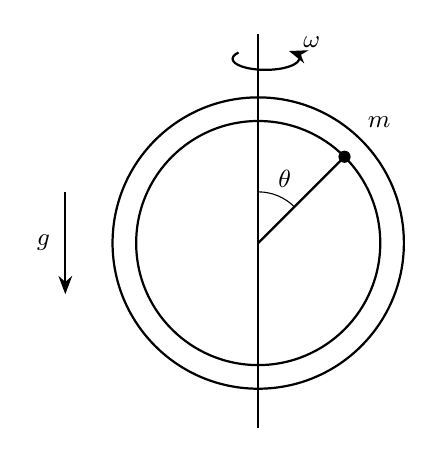
\begin{tikzpicture}[>=Stealth, font=\small]
  \def\R{1.85}
  \def\r{1.55}
  \def\rmid{1.70}
  \def\ang{45}

  % Concentric circular tube
  \draw[thick] (0,0) circle (\R);
  \draw[thick] (0,0) circle (\r);

  % Vertical rotation axis
  \draw[thick] (0,-2.35) -- (0,2.65);

  % Rotation arrow and omega
  \draw[->, thick] (-0.25,2.42) arc (145:405:0.42 and 0.14);
  \node[right=2pt] at (0.38,2.55) {$\omega$};

  % Gravity vector on the left
  \draw[->, thick] (-2.45,0.65) -- (-2.45,-0.65);
  \node[left=2pt] at (-2.45,0) {$g$};

  % Radial line to mass m
  \coordinate (O) at (0,0);
  \coordinate (Top) at (0,1);
  \coordinate (M) at ({90-\ang}:\r);
  \draw[thick] (O) -- (M);
  \fill (M) circle (2.2pt);
  \node at ({90-\ang}:{\R+0.32}) {$m$};

  % Angle theta
  \pic[draw, angle radius=0.65cm, angle eccentricity=1.35, "$\theta$"] {angle=M--O--Top};
\end{tikzpicture}

\end{center}
\end{problem}
\clearpage


\begin{problem}{2.2.7}
找出与下列势能函数相应的力场：

(1) $V = \frac{1}{2}\ln (x^2 +y^2 +z^2);$ 

(2) $V(r, \theta, \varphi) = \frac{1}{r} \mathrm{e}^{-kr}$ ; 

(3) $V(r, \theta, \varphi) = \frac{a}{r^2} \cos \theta$ .
\end{problem}
\clearpage


\begin{problem}{2.2.8}
证明一个半径为 $a$ 、面密度为 $\sigma$ 的薄圆盘，圆盘的轴向距离为 $x$ 的点的引力势为

\[
V (x) = - 2 \pi G \sigma (\sqrt {x ^ {2} + a ^ {2}} - | x |)
\]
\end{problem}
\clearpage


\begin{problem}{2.2.9}
计算半径为 a、质量为 M 的均质圆环对位于环的平面内，但在环的外侧的各点的引力势.

提示: 可表示为第一类椭圆积分.
\begin{center}
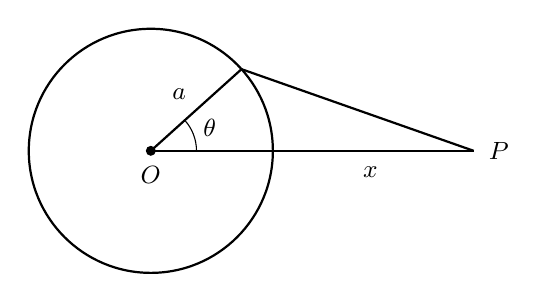
\begin{tikzpicture}[>=Stealth, font=\small]
  \def\a{1.55}
  \def\x{4.1}
  \def\ang{42}

  \coordinate (O) at (0,0);
  \coordinate (A) at (\ang:\a);
  \coordinate (P) at (\x,0);

  % Ring
  \draw[thick] (O) circle (\a);

  % Center O
  \fill (O) circle (1.8pt);
  \node[below=2pt] at (O) {$O$};

  % Triangle sides
  \draw[thick] (O) -- (A) node[midway, above left=0pt] {$a$};
  \draw[thick] (O) -- (P) node[pos=0.68, below=2pt] {$x$};
  \draw[thick] (A) -- (P);

  % Point P
  \node[right=2pt] at (P) {$P$};

  % Angle theta
  \pic[draw, angle radius=0.58cm, angle eccentricity=1.38, "$\theta$"] {angle=P--O--A};
\end{tikzpicture}

\end{center}
\end{problem}
\clearpage


\begin{problem}{2.2.10}
考虑一个任意形状的物体,证明:对物体外一个球内各点的引力势的平均值等于在此球心处的引力势.
\end{problem}
\clearpage


\begin{problem}{2.2.11}
判断以下各力是否是保守力,如果是保守力,找出它的势能函数.

(1) $F=(ax+by^{2})i+(az+2bxy)j+(ay+bz^{2})k,a,b$ 为常量；

(2) $F=a\times r,a$ 为常矢量；

(3) $F = ar, a$ 为常量；

(4) $F=a(a\cdot r)$ ,a为常矢量.
\end{problem}
\clearpage


\begin{problem}{2.2.12}
一个密度均匀的行星绕一个固定轴以角速度 $\omega$ 自转，行星的赤道半径 $R_{\mathrm{E}}$ 略大于球的半径 $R$ ，行星两极的半径 $R_{\mathrm{P}}$ 略小于球的半径 $R$ ，用参量 $\varepsilon = \frac{R_{\mathrm{E}} - R_{\mathrm{P}}}{R_{\mathrm{E}}}$ 描述变形的大小.由于这种变形引起重力势有一增量

\[
\Delta V (R, \theta) = - \frac {2}{5} \frac {G M \varepsilon R _ {\mathrm{E}} ^ {2}}{R ^ {3}} P _ {2} (\cos \theta)
\]

其中 $\theta$ 是球坐标， $P_{2}(\cos \theta) = \frac{3}{2}\cos^{2}\theta - \frac{1}{2}$ . 由行星表面平衡的条件得出 $\varepsilon$ 与 $\lambda = \frac{\omega^2 R_E}{g}$ 的关系，对地球就 $\varepsilon$ 作数值估计.
\end{problem}
\clearpage


\begin{problem}{2.2.13}
求在势能为

\[
V (x) = \frac {1}{2} k x ^ {2} - \frac {1}{3} m \lambda x ^ {3}
\]

(其中 $\lambda$ 很小) 的保守力作用下的非线性振子的运动的一级近似解, 假定 t=0 时 x=0.
\end{problem}
\clearpage


\begin{problem}{2.2.14}
(1) 质量为 $m$ 的粒子在势能 $V(x) = \frac{cx}{x^2 + a^2}$ 的保守力场中运动, 其中 $c$ 和 $a$ 是正的常数. 求稳定平衡位置及在它附近做小振动的周期.

(2) 如果粒子从所求的平衡位置以速度 v 开始运动, 求 v 值的范围, 粒子将做: (a) 振动; (b) 逃到 $-\infty$ ; (c) 逃到 $+\infty$ .
\end{problem}
\clearpage


\begin{problem}{2.2.15}
比地面高 h 的平台上有一质量为 m 的小车系于绳子一端, 绳子跨过一小滑轮在另一端被地面上的人拉着并以匀速 $v_{0}$ 向右运动，如图2.58所示.若小车与平台间的摩擦力可以不计，求：

(1) 当人位于离小滑轮正下方向右距离 s 处小车的速度和加速度；

(2) 人在上述位置拉绳的力；

(3) 在人从滑轮正下方到上述位置的过程中人所做的功.
\begin{center}
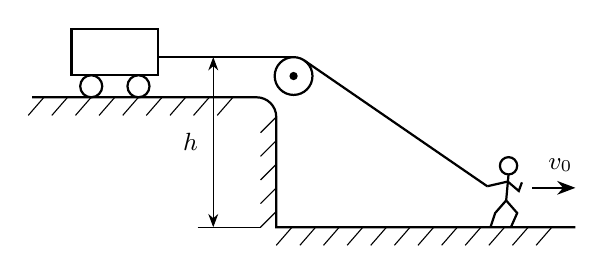
\begin{tikzpicture}[>=Stealth, font=\small]
  % Platform and lower ground
  \draw[thick] (-3.1,1.65) -- (-0.25,1.65) arc (90:0:0.25) -- (0,0) -- (3.8,0);

  % Hatching for platform, wall, and ground
  \foreach \x in {-2.95,-2.65,...,-0.25} {
    \draw (\x,1.65) -- (\x-0.2,1.42);
  }
  \foreach \y in {0.2,0.5,0.8,1.1,1.4} {
    \draw (0,\y) -- (-0.2,\y-0.2);
  }
  \foreach \x in {0.2,0.5,...,3.6} {
    \draw (\x,0) -- (\x-0.2,-0.23);
  }

  % Pulley
  \coordinate (Pul) at (0.22,1.92);
  \def\rp{0.24}
  \draw[thick] (Pul) circle (\rp);
  \fill (Pul) circle (1.5pt);

  % Cart
  \draw[thick] (-2.6,1.93) rectangle (-1.5,2.52);
  \draw[thick] (-2.35,1.79) circle (0.14);
  \draw[thick] (-1.75,1.79) circle (0.14);

  % Rope from cart to pulley top
  \pgfmathsetmacro{\yrope}{1.92+\rp}
  \draw[thick] (-1.5,\yrope) -- (0.22,\yrope);

  % Exact tangent from person's hand (2.68,0.52) to pulley
  \coordinate (Hand) at (2.68,0.52);
  \pgfmathsetmacro{\dx}{2.68-0.22}
  \pgfmathsetmacro{\dy}{0.52-1.92}
  \pgfmathsetmacro{\dist}{sqrt(\dx*\dx+\dy*\dy)}
  \pgfmathsetmacro{\baseang}{atan2(\dy,\dx)}
  \pgfmathsetmacro{\offsetang}{acos(\rp/\dist)}
  \pgfmathsetmacro{\tang}{\baseang+\offsetang}
  \coordinate (TanPt) at ($(Pul)+(\tang:\rp)$);
  \draw[thick] (TanPt) -- (Hand);

  % Height dimension h
  \draw (-1.0,0) -- (-0.2,0);
  \draw[<->] (-0.8,0) -- (-0.8,\yrope) node[midway, left=2pt] {$h$};

  % Person pulling the rope
  \draw[thick] (2.95,0.78) circle (0.11); % head
  \draw[thick] (2.95,0.67) -- (2.92,0.34); % torso
  \draw[thick] (2.94,0.58) -- (Hand); % back arm holding rope
  \draw[thick] (2.94,0.58) -- (3.08,0.46) -- (3.12,0.57); % front arm
  \draw[thick] (2.92,0.34) -- (2.78,0.18) -- (2.72,0); % back leg
  \draw[thick] (2.92,0.34) -- (3.06,0.18) -- (2.98,0); % front leg

  % Velocity arrow v_0
  \draw[->, thick] (3.25,0.50) -- (3.80,0.50) node[above=2pt, pos=0.65] {$v_0$};
\end{tikzpicture}

\end{center}
\end{problem}
\clearpage


\begin{problem}{2.2.16}
一质量为 $m$ 的小球系于不可伸长的轻绳的一端，穿过桌面上的一小孔后在光滑的水平桌面上运动，绳子与小孔间无摩擦力。问：

(1) 要使小球以小孔为中心做半径为 $r_{1}$ 、角速度为 $\omega_{1}$ 的圆周运动，绳的另一端需用多大的拉力？

(2) 要使小球圆周运动的半径从 $r=r_{1}$ 缩小到 $r=r_{2}$ ，拉力需做多大的功？
\end{problem}
\clearpage


\begin{problem}{2.2.17}
火车质量为 $m$ ，其所产生功率为常数 $P$ ，若车受的阻力为常数 $f$ ，试证时间与速度的关系为 $t = \frac{mP}{f^2} \ln \frac{P}{P - fv} - \frac{mv}{f}$ ；若所受阻力与速度 $v$ 成正比，则 $t = \frac{mv}{2f} \ln \frac{P}{P - fv}$ .
\end{problem}
\clearpage


\begin{problem}{2.2.18}
一质量为 $m$ 的质点, 受引力作用在一直线上运动. 当 $x \geqslant a$ 时, 引力值为 $m\mu a^2 / x^2$ ; 当 $x \leqslant a$ 时, 引力值为 $m\mu x / a$ , 式中 $x$ 是相对于线上某一点 (取为原点) 的距离, $\mu$ 及 $a$ 为常量. 如质点在离原点 $2a$ 处从静止开始运动, 求到达原点时的速度及走此段路程所需的时间.
\end{problem}
\clearpage


\begin{problem}{2.2.19}
轴套 A 的质量为 0.5kg，沿着位于铅垂平面的螺线形杆无摩擦地滑动。螺线形方程为 $r=0.3\theta$ ，式中 r 以米计， $\theta$ 以弧度计，轴套在大小不变的径向力 T=10N 作用下，从 A 点静止释放，滑到位置 B 处（见图 2.60）。求轴套到达 B 处时的速度。
\begin{center}
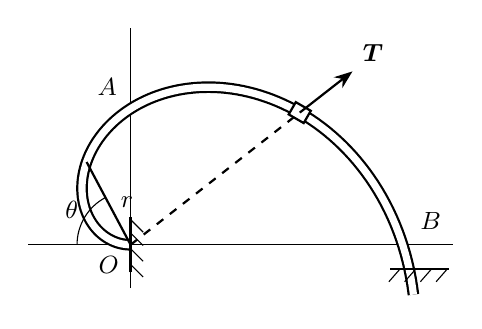
\begin{tikzpicture}[>=Stealth, font=\small]
  \def\c{1.1}
  \def\w{0.055}

  % Axes
  \draw (-1.3,0) -- (4.1,0);
  \draw (0,-0.55) -- (0,2.75);
  \node[below left=1pt] at (0,0) {$O$};

  % Spiral rod center path: x(t) = -c*t*cos(t), y(t) = c*t*sin(t)
  % Draw inner and outer boundaries as a smooth double-walled tube
  \draw[thick, double=white, double distance=2.6pt, samples=120, domain=0:190]
    plot ({-\c*(\x*pi/180)*cos(\x)}, {\c*(\x*pi/180)*sin(\x)});

  % Hatching support at O
  \draw[thick] (0,-0.35) -- (0,0.35);
  \foreach \y in {-0.25,-0.05,0.15,0.32} {
    \draw (0,\y) -- (0.16,\y-0.16);
  }

  % Hatching base below B
  \draw[thick] (3.3,-0.31) -- (4.05,-0.31);
  \foreach \x in {3.42,3.62,3.82,4.02} {
    \draw (\x,-0.31) -- (\x-0.14,-0.47);
  }

  % Point A (theta = 90 deg) and Point B (theta = 180 deg)
  \pgfmathsetmacro{\yA}{\c*pi/2}
  \pgfmathsetmacro{\xB}{\c*pi}
  \node[above left=2pt] at (0,\yA) {$A$};
  \node[above right=2pt] at (\xB+0.05,0.02) {$B$};

  % Radial segment r at theta = 62 deg
  \def\thOne{62}
  \pgfmathsetmacro{\rOne}{\c*\thOne*pi/180}
  \coordinate (O) at (0,0);
  \coordinate (NegX) at (-1,0);
  \coordinate (Pone) at ({-\rOne*cos(\thOne)}, {\rOne*sin(\thOne)});
  \draw[thick] (O) -- (Pone) node[pos=0.52, right=1pt] {$r$};
  \pic[draw, angle radius=0.68cm, angle eccentricity=1.28, "$\theta$"] {angle=Pone--O--NegX};

  % Collar / sleeve and radial force T at theta = 142 deg
  \def\thTwo{142}
  \pgfmathsetmacro{\rTwo}{\c*\thTwo*pi/180}
  \pgfmathsetmacro{\px}{-\rTwo*cos(\thTwo)}
  \pgfmathsetmacro{\py}{\rTwo*sin(\thTwo)}
  % Tangent angle of spiral at theta = 142 deg
  \pgfmathsetmacro{\dx}{-\c*(cos(\thTwo)-(\thTwo*pi/180)*sin(\thTwo))}
  \pgfmathsetmacro{\dy}{\c*(sin(\thTwo)+(\thTwo*pi/180)*cos(\thTwo))}
  \pgfmathsetmacro{\tang}{atan2(\dy,\dx)}

  \coordinate (Ptwo) at (\px,\py);
  \coordinate (Ttip) at ({\px+0.85*(-cos(\thTwo))}, {\py+0.85*sin(\thTwo)});
  \draw[dashed, thick] (O) -- (Ptwo);

  % Sleeve around the spiral rod at Ptwo
  \begin{scope}[shift={(Ptwo)}, rotate=\tang]
    \draw[thick, fill=white] (-0.11,-0.09) rectangle (0.11,0.09);
  \end{scope}

  \draw[->, thick] (Ptwo) -- (Ttip) node[above right=0pt] {$\boldsymbol{T}$};
\end{tikzpicture}

\end{center}
\end{problem}
\clearpage


\begin{problem}{2.2.20}
一质量为 80kg 的人由 1m 高处跳下, 当他落地时, 他忘了弯曲他的膝盖, 人体减速的距离只有 1cm. 求在减速阶段, 作用在他腿上的力.
\end{problem}
\clearpage


\begin{problem}{2.2.21}
一质点无摩擦地在环形轨道上滑下,如图 2.61 所示,轨道弯曲段的曲率半径为 R,该质点由高 h 处由自静止开始下滑,在某处质点开始和轨道脱离接触,说明脱离接触的位置并计算出发生这种情况的 h 的最小值.
\begin{center}
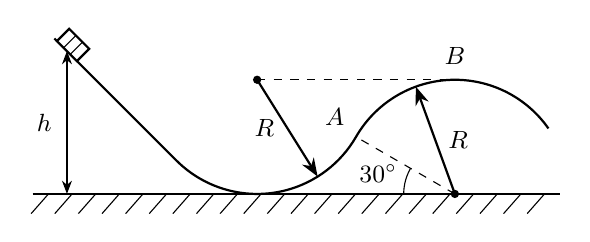
\begin{tikzpicture}[>=Stealth, font=\small]
  \def\R{1.45}
  \pgfmathsetmacro{\xCtwo}{\R*sqrt(3)}
  \pgfmathsetmacro{\xA}{\R*sqrt(3)/2}
  \pgfmathsetmacro{\yA}{\R/2}

  \coordinate (C1) at (0,\R);
  \coordinate (C2) at (\xCtwo,0);
  \coordinate (A) at (\xA,\yA);
  \coordinate (B) at (\xCtwo,\R);

  % Ground
  \draw[thick] (-2.85,0) -- (3.85,0);
  \foreach \x in {-2.65,-2.35,...,3.75} {
    \draw (\x,0) -- (\x-0.22,-0.25);
  }

  % Left incline + valley arc (225 deg to 330 deg around C1) + hill arc (150 deg down to 35 deg around C2)
  \coordinate (JoinL) at ($(C1)+(225:\R)$);
  \coordinate (TopL) at ($(JoinL)+(-1.55,1.55)$);
  \draw[thick] (TopL) -- (JoinL)
    arc (225:330:\R)
    arc (150:35:\R);

  % Block near top of left incline (rotated -45 deg)
  \coordinate (Blk) at ($(TopL)+(0.16,-0.16)$);
  \begin{scope}[shift={(Blk)}, rotate=-45]
    \draw[thick, fill=white] (-0.18,0) rectangle (0.18,0.22);
    \draw (-0.06,0) -- (-0.06,0.22) (0.06,0) -- (0.06,0.22);
  \end{scope}

  % Height h arrow
  \draw[<->] (Blk |- 0,0) -- (Blk) node[midway, left=2pt] {$h$};

  % Centers, dashed construction lines, and radius arrows
  \fill (C1) circle (1.5pt);
  \fill (C2) circle (1.5pt);
  \draw[dashed] (C1) -- (B);
  \draw[dashed] (C2) -- (A);

  % Radius arrows labeled R
  \draw[->, thick] (C1) -- ($(C1)+(302:\R)$) node[midway, left=1pt] {$R$};
  \draw[->, thick] (C2) -- ($(C2)+(110:\R)$) node[midway, right=1pt] {$R$};

  % Angle 30 deg at C2
  \coordinate (LeftG) at (0,0);
  \pic[draw, angle radius=0.65cm, angle eccentricity=1.55, "$30^\circ$"] {angle=A--C2--LeftG};

  % Labels A and B
  \node[above left=1pt] at (A) {$A$};
  \node[above=2pt] at (B) {$B$};
\end{tikzpicture}

\end{center}
\end{problem}
\clearpage


\begin{problem}{2.2.22}
一个转动的球形行星, 其赤道上的点的速率为 $V$ , 赤道上的 $g$ 是两极处 $g$ 的一半. 问粒子从极点逃逸的逃逸速度多大?
\end{problem}
\clearpage


\begin{problem}{2.2.23}
一跳伞员在 3000m 高处起跳. 在降落伞张开之前他达到一极限速度 30m/s.

(1) 假定空气阻力正比于速度,他达到这个极限速度需多久?达到这个速度时,运行了多少距离?

(2) 为了经受一个不大于 $10g(g$ 为重力加速度)的减速度, 在他的伞张开以后, 当他碰到地面时, 速度已降到 $3m/s$ , 他弯曲膝部以减缓冲撞, 需将膝部弯曲多少? 假定他的膝部像弹簧一样具有正比于位移的阻力.

(3) 空气阻力正比于速度的假定是否合理?
\end{problem}
\clearpage


\begin{problem}{2.2.24}
一个光滑球固定在水平面上, 一个点粒子在最高点从静止开始沿球面滑下. 令球的半径为 R, 描述粒子落到平面以前的路径 (见图 2.62).
\begin{center}
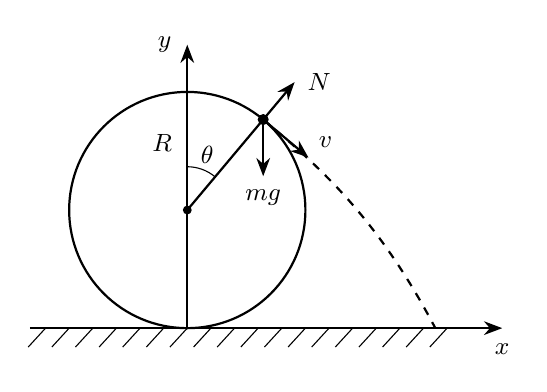
\begin{tikzpicture}[>=Stealth, font=\small]
  \def\R{1.5}
  \def\th{40}

  % Ground / x-axis
  \draw[->, thick] (-2.0,0) -- (4.0,0) node[below=2pt] {$x$};
  \foreach \x in {-1.8,-1.5,...,3.6} {
    \draw (\x,0) -- (\x-0.22,-0.24);
  }

  % Sphere
  \coordinate (C) at (0,\R);
  \draw[thick] (C) circle (\R);
  \fill (C) circle (1.6pt);

  % y-axis
  \draw[->, thick] (0,0) -- (0,3.6) node[left=2pt] {$y$};
  \node[left=2pt] at (0,2.35) {$R$};

  % Particle on sphere at angle th from top vertical
  \coordinate (Top) at (0,2*\R);
  \coordinate (P) at ($(C)+({90-\th}:\R)$);
  \draw[thick] (C) -- (P);
  \fill (P) circle (2pt);

  % Angle theta
  \pic[draw, angle radius=0.55cm, angle eccentricity=1.35, "$\theta$"] {angle=P--C--Top};

  % Force & velocity arrows at P
  \draw[->, thick] (P) -- ($(P)+({90-\th}:0.62)$) node[right=1pt] {$N$};
  \draw[->, thick] (P) -- ($(P)+(0,-0.72)$) node[below=1pt] {$mg$};
  \draw[->, thick] (P) -- ($(P)+(-\th:0.75)$) node[above right=0pt] {$v$};

  % Parabolic trajectory after leaving sphere
  \draw[dashed, thick] (P) .. controls ($(P)+(-\th:0.95)$) and ($(P)+(1.45,-1.25)$) .. (3.15,0);
\end{tikzpicture}

\end{center}
\end{problem}
\clearpage


\begin{problem}{2.2.25}
若在北京和天津间用一条直的地下铁道联结, 如图 2.63 所示, 两市间的火车在地球引力作用下运行, 两市间直线距离为 $130\mathrm{km}$ , 地球半径 $R = 6400\mathrm{km}$ . 忽略摩擦, 计算火车的最大速度以及从北京到天津坐此火车所需的时间.
\begin{center}
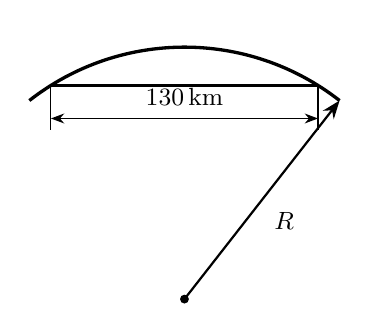
\begin{tikzpicture}[>=Stealth, font=\small]
  \def\R{3.2}
  \def\aEnd{52}
  \def\aChord{58}

  \coordinate (O) at (0,0);
  \fill (O) circle (1.6pt);

  % Earth surface arc
  \draw[very thick] (\aEnd:\R) arc (\aEnd:{180-\aEnd}:\R);

  % Straight tunnel chord
  \coordinate (P1) at ({180-\aChord}:\R);
  \coordinate (P2) at (\aChord:\R);
  \draw[thick] (P1) -- (P2);

  % Dimension 130km
  \pgfmathsetmacro{\yCh}{\R*sin(\aChord)}
  \pgfmathsetmacro{\xCh}{\R*cos(\aChord)}
  \draw (-\xCh,\yCh) -- (-\xCh,\yCh-0.56);
  \draw (\xCh,\yCh) -- (\xCh,\yCh-0.56);
  \draw[<->] (-\xCh,\yCh-0.42) -- (\xCh,\yCh-0.42) node[midway, above=1pt] {$130\,\mathrm{km}$};

  % Radius arrow R
  \draw[->, thick] (O) -- (\aEnd:\R) node[midway, below right=1pt] {$R$};
\end{tikzpicture}

\end{center}
\end{problem}
\clearpage


\begin{problem}{2.2.26}
估计一下通过跳跃就能脱离的小行星多大.
\end{problem}
\clearpage


\begin{problem}{2.2.27}
求:(1)月球表面的重力加速度;(2)从月球表面出发逃离月球所需的最小速度.月球质量为 $7.35\times10^{22}kg$ ,月球半径为 $1.74\times10^{3}km$ .
\end{problem}
\clearpage


\begin{problem}{2.2.28}
一质量为 m 的质点从置于光滑水平面上的、质量为 M 的光滑的、半径为 R 的弧形槽的顶端滑下，如图 2.65 所示。开始滑下时，m、M 都是静止的，求质点离开弧形槽时质点和弧形槽的速度。
\begin{center}
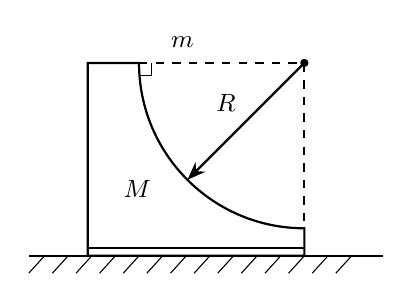
\begin{tikzpicture}[>=Stealth, font=\small]
  \def\R{2.1}
  \def\hbase{0.35}
  \def\topY{2.45} % hbase + R

  % Ground
  \draw[thick] (-0.4,0) -- (4.1,0);
  \foreach \x in {-0.2,0.1,...,3.9} {
    \draw (\x,0) -- (\x-0.2,-0.22);
  }

  % Block M with quarter-circle track
  % Center of arc at (3.1, 2.45), left top lip at (1.0, 2.45), bottom lip at (3.1, 0.35)
  \draw[thick] (0.35,0) -- (0.35,\topY) -- (1.0,\topY)
    arc (180:270:\R) -- (3.1,0) -- cycle;
  % Base step line
  \draw (0.35,0.1) -- (3.1,0.1);

  % Center of curvature and dashed lines
  \coordinate (C) at (3.1,\topY);
  \fill (C) circle (1.5pt);
  \draw[dashed, thick] (1.0,\topY) -- (C) -- (3.1,\hbase);

  % Right-angle mark at top lip
  \draw (1.0,{\topY-0.16}) -- (1.16,{\topY-0.16}) -- (1.16,\topY);

  % Radius arrow R
  \draw[->, thick] (C) -- ($(C)+(225:\R)$) node[midway, above left=0pt] {$R$};

  % Labels m and M
  \node[above=2pt] at (1.55,\topY) {$m$};
  \node at (0.98,0.85) {$M$};
\end{tikzpicture}

\end{center}
\end{problem}
\clearpage


\begin{problem}{2.2.29}
如图 2.66 所示, 小球质量为 m, 连接在绕水平轴 O 旋转的 BD 杆的 D 端, 连杆 BC 穿过绕 A 点转动的套筒, 并能在其内滑动, 劲度系数为 k 的弹簧套在 BC 杆的 AC 段, 当球下降时压缩弹簧, $\theta = 60^{\circ}$ 的位置时, 弹簧无伸缩. 从此位置静止释放, 求 $\theta = 90^{\circ}$ 时 BC 杆的角速度. 设 BC 杆及 BD 杆的质量及各处摩擦可略去不计.
\begin{center}
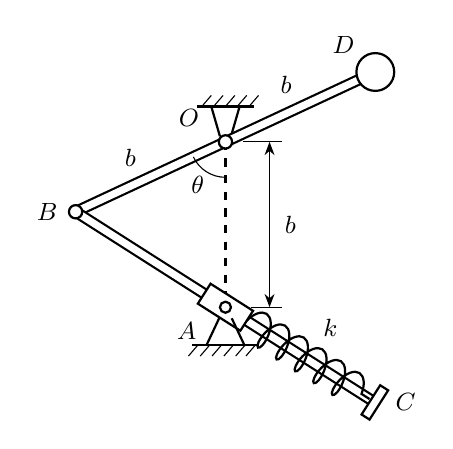
\begin{tikzpicture}[>=Stealth, font=\small]
  \def\b{2.1}
  \def\th{65}

  \coordinate (O) at (0,0);
  \coordinate (A) at (0,-\b);
  \coordinate (B) at ({-\b*sin(\th)}, {-\b*cos(\th)});
  \coordinate (D) at ({\b*sin(\th)}, {\b*cos(\th)});

  % Ceiling support at O
  \draw[thick] (-0.36,0.45) -- (0.36,0.45);
  \foreach \x in {-0.30,-0.15,0.0,0.15,0.30} {
    \draw (\x,0.45) -- (\x+0.12,0.59);
  }
  \draw[thick] (-0.18,0.45) -- (-0.07,0.07);
  \draw[thick] (0.18,0.45) -- (0.07,0.07);

  % Rod BD
  \draw[thick, double=white, double distance=2.6pt] (B) -- (D);
  \node[above left=1pt] at ($(O)!0.52!(B)$) {$b$};
  \node[above left=1pt] at ($(O)!0.52!(D)$) {$b$};

  % Mass sphere at D
  \draw[thick, fill=white] (D) circle (0.24);
  \node[above left=3pt and 4pt] at (D) {$D$};

  % Vertical dashed line OA and dimension b
  \draw[dashed, thick] (O) -- (A);
  \draw (0.22,0) -- (0.72,0);
  \draw (0.32,-\b) -- (0.72,-\b);
  \draw[<->] (0.56,0) -- (0.56,-\b) node[midway, right=2pt] {$b$};

  % Angle theta
  \pic[draw, angle radius=0.45cm, angle eccentricity=1.45, "$\theta$"] {angle=B--O--A};

  % Rod BC direction from B through A to C
  \pgfmathsetmacro{\dx}{0 - (-\b*sin(\th))}
  \pgfmathsetmacro{\dy}{-\b - (-\b*cos(\th))}
  \pgfmathsetmacro{\angBA}{atan2(\dy,\dx)}
  \coordinate (C) at ($(A)+(\angBA:2.25)$);

  % Rod BC (double line)
  \draw[thick, double=white, double distance=2.6pt] (B) -- (C);

  % Spring along AC (from sleeve exit to plate C)
  \coordinate (SpStart) at ($(A)+(\angBA:0.32)$);
  \coordinate (SpEnd) at ($(C)+(\angBA:-0.08)$);
  \draw[thick, decorate, decoration={coil, aspect=0.45, segment length=2.8mm, amplitude=2.1mm}]
    (SpStart) -- (SpEnd);
  \node[above right=5pt and 2pt] at ($(SpStart)!0.5!(SpEnd)$) {$k$};

  % End plate at C
  \begin{scope}[shift={(C)}, rotate=\angBA]
    \draw[thick, fill=white] (-0.06,-0.22) rectangle (0.06,0.22);
  \end{scope}
  \node[right=4pt] at (C) {$C$};

  % Sleeve at A
  \begin{scope}[shift={(A)}, rotate=\angBA]
    \draw[thick, fill=white] (-0.32,-0.15) rectangle (0.32,0.15);
  \end{scope}

  % Floor support at A
  \draw[thick] (-0.42,-\b-0.48) -- (0.42,-\b-0.48);
  \foreach \x in {-0.35,-0.20,-0.05,0.10,0.25,0.38} {
    \draw (\x,-\b-0.48) -- (\x-0.12,-\b-0.62);
  }
  \draw[thick] (-0.24,-\b-0.48) -- (-0.08,-\b-0.14);
  \draw[thick] (0.24,-\b-0.48) -- (0.08,-\b-0.14);

  % Pivot pins at O, B, A
  \draw[thick, fill=white] (O) circle (2.4pt);
  \draw[thick, fill=white] (B) circle (2.4pt);
  \draw[thick, fill=white] (A) circle (2.0pt);

  \node[above left=2pt and 6pt] at (O) {$O$};
  \node[left=3pt] at (B) {$B$};
  \node[below left=2pt and 7pt] at (A) {$A$};
\end{tikzpicture}

\end{center}
\end{problem}
\clearpage


\begin{problem}{2.2.30}
求质量为 $m$ 和具有能量 $E$ 的质点在势场 $V = V_{0}\tan^{2}ax$ (式中 $V_{0}$ 和 $a$ 为常量) 中做一维运动的周期.
\end{problem}
\clearpage


\begin{problem}{2.2.31}
一根长度为 $a$ 的不可伸长的轻绳，一端连着一个质量为 $m$ 的粒子 $P$ ，另一端连着一个质量为 $\frac{3}{2} m$ 的环 $Q$ ，此环穿在一根固定的粗糙的水平的金属丝上。从环和粒子处于平衡的状态给粒子一个沿水平方向的速度 $\sqrt{2ag}$ ，证明：在小环不在金属丝上滑动的情况下，绳中张力为 $3mg\cos \theta$ ，其中 $\theta$ 是绳子与铅垂线间的夹角；并证明：如环与金属丝间摩擦因数大于 $\frac{1}{\sqrt{3}}$ ，环就不会滑动。
\end{problem}
\clearpage


\begin{problem}{2.2.32}
一质点自一光滑的抛物线上一点 $Q$ 自由滑下, 该点在轴线上方 $h$ 处, 抛物线的方程为 $y^{2} = 2px$ , $y$ 轴竖直向上. 问质点滑至何处时, 曲线对质点的约束力将改变符号 (求出此点的 $y$ 坐标满足的方程即可).
\end{problem}
\clearpage


\begin{problem}{2.2.33}
一个质点在恒定的重力作用下在 $xy$ 平面内运动, 重力沿 $y$ 轴负方向. 找出该二维运动的四个独立的运动常数, 其中有三个独立的运动常数不显含时间.
\end{problem}
\clearpage


\begin{problem}{2.2.34}
当一个正在收缩的星体收缩到它的 Schwarzschild 半径 $R_{s}$ 以下时, 它变成一个黑洞, 光和任何粒子都不能逃离它. 导出 $R_{s}$ 和它的质量 M 的关系.
\end{problem}
\clearpage


\section{质点的角动量定理和角动量守恒定律}

\begin{problem}{2.3.1}
一质量为 m 的质点在光滑水平面上以速率 $v_{0}$ 做半径为 $R_{0}$ 的圆周运动。该质点系在一根不可伸长的轻绳上，绳子又穿过该平面上的一个光滑小孔，如图 2.69 所示。

(1) 绳中的张力多大?

(2) 质点对小孔的角动量多大?

(3) 质点的动能多大?

(4) 若使绳中的张力逐渐地增大, 最后使质点做

半径为 $\frac{1}{2} R_0$ 的圆周运动，质点最终的动能多大？

(5) 如果张力不是逐渐增大, 上问的答案还对吗?
\begin{center}
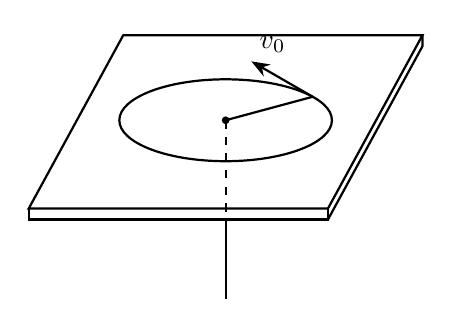
\begin{tikzpicture}[>=Stealth, thick]
  % Horizontal plane (top face and front/right thickness)
  \draw[fill=white] (-2.2,-1.1) -- (1.6,-1.1) -- (2.8,1.1) -- (-1.0,1.1) -- cycle;
  \draw (-2.2,-1.1) -- (-2.2,-1.24) -- (1.6,-1.24) -- (1.6,-1.1);
  \draw (1.6,-1.24) -- (2.8,0.96) -- (2.8,1.1);

  % Circular orbit in perspective
  \coordinate (O) at (0.3,0.02);
  \draw (O) ellipse [x radius=1.35, y radius=0.52];
  \fill (O) circle (1.4pt);

  % Point on orbit, radius string, and tangential velocity
  \coordinate (P) at ($(O) + (35:1.35 and 0.52)$);
  \draw (O) -- (P);
  \draw[->] (P) -- ++(-0.78, 0.45) node[above right=-1pt] {$v_0$};

  % Vertical string passing through the hole
  \draw[dashed] (O) -- (0.3,-1.24);
  \draw (0.3,-1.24) -- (0.3,-2.25);
\end{tikzpicture}

\end{center}
\end{problem}
\clearpage


\begin{problem}{2.3.2}
一质量为 $m$ 的小孩坐在一秋千上, 秋千的质量可以忽略, 悬挂在一端固定的、长度为 $l$ 的绳的另一端. 小孩的父亲拉他的后背使绳子和铅直方向的夹角为 $1\mathrm{rad}$ , 然后以力 $F = mg$ 沿圆周的切线方向推小孩直到绳子到达铅直位置放开该秋千. 问孩子的父亲推秋千用了多少时间? 在 $\theta < 1\mathrm{rad}$ 时可作近似 $\sin \theta \approx \theta$ .
\end{problem}
\clearpage


\begin{problem}{2.3.3}
一质量为 $m$ 的质点受到两个力的作用, $\bm{F}_1 = f(r)\bm{e}_r$ , $\bm{F}_2 = -\lambda \bm{v} (\lambda > 0$ , 为常量), $\bm{v}$ 是质点的速度. 若该质点初始时对原点的角动量为 $\bm{J}_0$ , 求以后时刻它对原点的角动量.
\end{problem}
\clearpage


\begin{problem}{2.3.4}
一质量为 m 的粒子, 在半顶角为 $\alpha$ 的锥体内表面无摩擦地滑动.

(1) 找出使该质点绕竖直轴做圆轨道运动在初始条件方面的要求；

(2) 说明这种轨道运动是否稳定,何故?
\end{problem}
\clearpage


\begin{problem}{2.3.5}
质量分别为 $m, 2m, 3m, 4m, 5m$ 的五个质点，用八根长度均为 $l$ 的轻质杆连成图2.71所示的锥体，以角速度 $\omega$ 绕连接 $4m$ 与 $5m$ 的线转动。求锥体对 $O$ 点的角动量的 $x, y, z$ 方向的分量。
\begin{center}
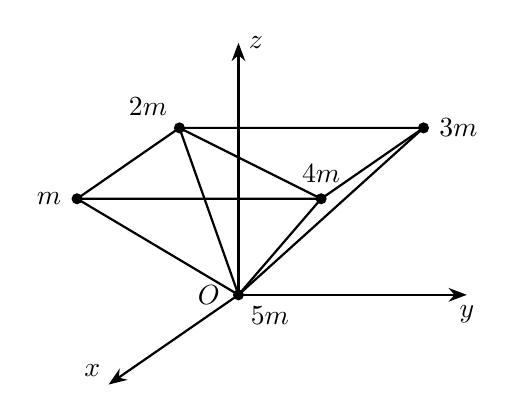
\begin{tikzpicture}[>=Stealth, thick]
  % Coordinate axes
  \coordinate (O) at (0,0);
  \draw[->] (O) -- (0,3.2) node[right] {$z$};
  \draw[->] (O) -- (2.9,0) node[below] {$y$};
  \draw[->] (O) -- (-1.65,-1.14) node[above left=-1pt] {$x$};

  % Pyramid vertices
  \coordinate (M1) at (-2.05,1.22);
  \coordinate (M2) at (-0.75,2.12);
  \coordinate (M3) at (2.35,2.12);
  \coordinate (M4) at (1.05,1.22);

  % Pyramid rods
  \draw (M1) -- (M2) -- (M3) -- (M4) -- cycle;
  \draw (M2) -- (M4);
  \draw (O) -- (M1);
  \draw (O) -- (M2);
  \draw (O) -- (M3);
  \draw (O) -- (M4);

  % Point masses and labels
  \fill (O) circle (2pt) node[left=3pt] {$O$} node[below right=1pt] {$5m$};
  \fill (M1) circle (2pt) node[left=2pt] {$m$};
  \fill (M2) circle (2pt) node[above left=1pt] {$2m$};
  \fill (M3) circle (2pt) node[right=2pt] {$3m$};
  \fill (M4) circle (2pt) node[above=2pt] {$4m$};
\end{tikzpicture}

\end{center}
\end{problem}
\clearpage


\begin{problem}{2.3.6}
一有方向的直线 $L$ ，其方向余弦为 $l, m, n$ ，且通过点 $(a, b, c)$ 。求在 $xy$ 平面上通过原点与 $x$ 轴夹角为 $\alpha$ 、与 $y$ 轴夹角为 $\frac{\pi}{2} - \alpha$ 的单位矢量对有向直线 $L$ 的矩。
\end{problem}
\clearpage


\begin{problem}{2.3.7}
(1) 如果加给 $n$ 个质点的所有力的矢量和等于零，证明：加给这 $n$ 个质点的力矩之矢量和与计算它的参考点（矩心）无关；

(2) 如果 n 个质点的动量之矢量和等于零, 证明: 这 n 个质点的角动量之矢量和与计算它的参考点(矩心)无关.

2.72 所示.
\end{problem}
\clearpage


\begin{problem}{2.3.8}
一个质点在重力作用下，沿一个对竖直轴对称的光滑旋转面上运动。用柱坐标表示的该旋转面的方程为 $\rho = f(z)$ 。如质点在高度 $z_{1}$ 处，速度是水平的、大小为 $v_{1}$ ，在高度 $z_{2}$ 处，速度再次是水平的、大小为 $v_{2}$ 。求 $v_{1}, v_{2}$ ，把它们写成 $z_{1}, z_{2}$ 的函数。
\end{problem}
\clearpage


\begin{problem}{2.3.9}
一个原长为 $a$ 、弹性模量为 $\lambda$ 的弹性绳一端固定在一个光滑水平面上的固定点 $O$ , 另一端系一个质量为 $m$ 的质点, 原先在平面上处于静止, 突然给质点施加一个大小为 $v$ 、方向垂直于绳的速度, 以后运动中, 绳被拉伸到最大长度 $3a$ . 求质点的初速度 $v$ .
\end{problem}
\clearpage


\begin{problem}{2.3.10}
质量为 $m$ 、带电量为 $e$ 的点电荷，在强度为 $g$ 的磁单极子场中运动，磁单极子可以看成无限重、位于原点，点电荷受磁单极子的作用力为 $-ge\frac{\dot{r} \times r}{r^3}$ ，不计重力。

(1) 证明动能 $T=\frac{1}{2}m\dot{r}\cdot\dot{r}$ 是运动积分；

(2) 证明 $L = J + \frac{eg}{r} r$ 是运动积分, 其中 $J = r \times m \dot{r}$ ;

(3) 利用上述 L 是运动积分, 证明这个带电粒子的运动轨道在一个半顶角为 $\alpha$ 的圆锥面上, L 是该圆锥的对称轴, $\alpha$ 满足 $\cos\alpha=\frac{eg}{|L|}$ .

提示:考虑 $r \cdot L$ .
\end{problem}
\clearpage


\begin{problem}{2.3.11}
两个同轴的长半圆筒, 其截面如图 2.74 所示, 分别带正、负电, 使其间电场为 $E = \frac{k}{r} e_r$ , (k 为常量), 一质量为 $m$ 、带电 $-q(q > 0)$ 的粒子, 从左方以垂直半圆筒的轴和垂直半径方向的速度 $v$ 进入两极之间, 如图 2.74 所示. 粒子将在图平面内运动.

(1) 如果粒子在两极间沿圆轨道运动, 其轨道半径 r 多大?

(2) 假定粒子进入场区时, 离轴的距离 $r$ 与速度 $\bm{v}$ 的大小均与 (1) 中相同, 但 $\bm{v}$ 的方向偏离一个小角 $\beta$ . 新轨道与 (1) 中的轨道将再次相交于 $P$ 点, $P$ 点的位置与 $\beta$ 无关, 求出 $P$ 点的位置 (粒子进入场区时仍没有轴向的分速度, 仍在图平面内运动).

(3) 如果把电场改为平行于半圆筒轴的均匀磁场, 粒子沿圆轨道运动, 轨道半径 r 多大?
\begin{center}
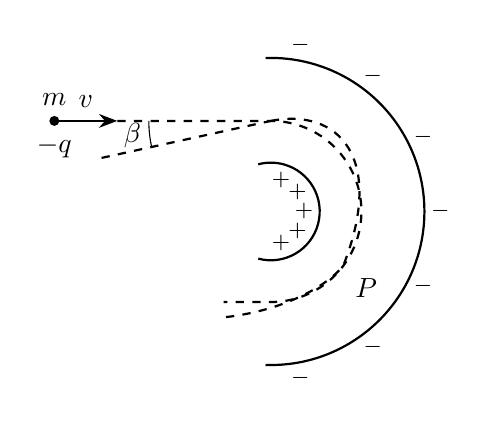
\begin{tikzpicture}[>=Stealth, thick]
  \coordinate (C) at (0.6,0);
  \def\Rout{1.95}
  \def\Rin{0.62}
  \def\Rorb{1.15}

  % Outer negatively charged half-cylinder
  \draw (C) ++(-92:\Rout) arc (-92:92:\Rout);
  \foreach \a in {-80,-53,-26,0,26,53,80} {
    \node[font=\footnotesize] at ($(C) + (\a:\Rout+0.20)$) {$-$};
  }

  % Inner positively charged half-cylinder
  \draw (C) ++(-105:\Rin) arc (-105:105:\Rin);
  \foreach \a in {-72,-36,0,36,72} {
    \node[font=\footnotesize] at ($(C) + (\a:\Rin-0.20)$) {$+$};
  }

  % Incident particle and velocity
  \coordinate (S) at (-2.15,\Rorb);
  \coordinate (E) at (0.6,\Rorb);
  \fill (S) circle (1.8pt) node[above=2pt] {$m$} node[below=2pt] {$-q$};
  \draw[->] (S) -- (-1.35,\Rorb) node[midway, above=1pt] {$v$};

  % Circular reference trajectory (dashed)
  \draw[dashed] (-1.35,\Rorb) -- (E)
    arc (90:-90:\Rorb) -- (0.0,-\Rorb);

  % Perturbed trajectory entering at small angle beta
  \coordinate (B0) at (-1.55,0.68);
  \draw[dashed] (B0) -- (E);

  % Angle beta between incident rays
  \coordinate (H) at (-1.35,\Rorb);
  \pic[draw, thin, angle radius=1.55cm, angle eccentricity=1.14, "$\beta$"] {angle = H--E--B0};

  % Perturbed trajectory inside field intersecting at P
  \coordinate (P) at ($(C) + (-37:\Rorb)$);
  \draw[dashed] (E)
    .. controls (1.46,1.32) and (2.06,0.68) .. (P)
    .. controls (1.28,-0.98) and (0.70,-1.28) .. (-0.05,-1.35);
  \node[below right=1pt] at (P) {$P$};
\end{tikzpicture}

\end{center}
\end{problem}
\clearpage


\begin{problem}{2.3.12}
证明: 在两个质量为 $m_{1}, m_{2}$ 的质点按库仑定律相互作用的问题中, 矢量 $L = V \times J + \frac{ar}{r}$ 是运动积分, 其中 $V$ 是相对速度, $r$ 是相对位矢, $J = \mu(r \times V)$ 是与相对运动相联系的角动量, $a$ 是库仑定律中的常系数, $\mu = \frac{m_1 m_2}{m_1 + m_2}$ .

提示:要考虑质点 2 相对于质点 1 的运动.
\end{problem}
\clearpage


\begin{problem}{2.3.13}
一宇宙飞船围绕质量为 $M$ 的恒星作半径为 $r_0$ 的圆周运动, 宇宙飞船的火箭可以迅速点燃, 使飞船速度瞬时改变 $\Delta v$ , 点燃的方位用飞船的速度 $v$ 和 $\Delta v$ 之间的夹角来说明, 如图 2.75 所示, 为了保存燃料, 在连续 $N$ 次发射中, 希望 $\Delta v = \sum_{i=1}^{N} |\Delta v_i|$ 减至最小, 称 $\Delta v$ 为比冲量.

（1）假如我们要利用飞船的火箭逃离这个恒星，且只点燃一次，需要的最小的比冲量多大？在什么方位点燃？

(2) 假如我们要在半径为 $r_{1}(>r_{0})$ 的圆轨道上视察一颗行星, 让火箭再次点燃, 达到该行星轨道所需的最小比冲量多大?

(3) 假如我们要用飞船的火箭使它撞上恒星(假定恒星的半径可以忽略), 对下列两种点火策略计算最小比冲量: (a) 在 $\theta = 180^{\circ}$ 一次迅速点燃; (b) 在 $\theta = 0^{\circ}$ 一次快速点燃, 然后在晚些时候在 $\theta = 180^{\circ}$ 第二次点燃, 为使总的比冲量最小, 选择第二次点火的时间和每次突发的强度.
\begin{center}
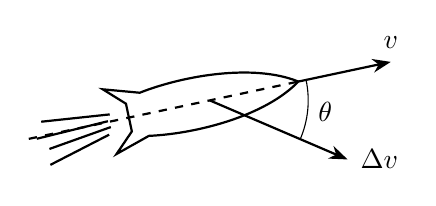
\begin{tikzpicture}[>=Stealth, thick]
  % Rocket body tilted slightly up-right
  \begin{scope}[rotate=12]
    \coordinate (C) at (0,0);
    \coordinate (Nose) at (1.15,0);
    % Streamlined fuselage with upper and lower fins
    \draw[fill=white]
      (-1.05,0.18) -- (-1.30,0.42) -- (-0.85,0.28)
      .. controls (-0.25,0.38) and (0.65,0.34) .. (Nose)
      .. controls (0.65,-0.34) and (-0.25,-0.38) .. (-0.85,-0.28)
      -- (-1.30,-0.42) -- (-1.05,-0.18) -- cycle;

    % Exhaust plumes behind nozzle
    \draw (-1.28,0.09) -- (-2.15,0.18);
    \draw (-1.32,0.01) -- (-2.25,-0.02);
    \draw (-1.30,-0.07) -- (-2.12,-0.18);
    \draw (-1.34,-0.16) -- (-2.15,-0.38);

    % Centerline and velocity vector v
    \draw[dashed] (-2.35,0) -- (Nose);
    \draw[->] (Nose) -- (2.35,0) node[above=1pt] {$v$};
    \coordinate (AxisF) at (2.0,0);
  \end{scope}

  % Velocity impulse vector Delta v
  \coordinate (DV) at (1.75,-0.75);
  \draw[->] (C) -- (DV) node[right=1pt] {$\Delta v$};

  % Angle theta between v and Delta v
  \pic[draw, thin, angle radius=1.25cm, angle eccentricity=1.18, "$\theta$"] {angle = DV--C--AxisF};
\end{tikzpicture}

\end{center}
\end{problem}
\clearpage


\section{碰 撞}

\begin{problem}{2.4.1}
一质量为 m 的子弹射入置于光滑水平面上质量为 M 并与劲度系数为 k 的轻弹簧连着的木块后使弹簧最大压缩了 L，求子弹射入前的速度 $v_{0}$ .
\begin{center}
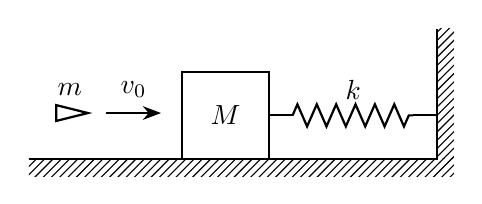
\begin{tikzpicture}[>=Stealth, thick]
  % Horizontal floor and right wall with hatching
  \fill[pattern=north east lines] (0,-0.22) rectangle (5.4,0);
  \fill[pattern=north east lines] (5.18,0) rectangle (5.4,1.65);
  \draw (0,0) -- (5.18,0) -- (5.18,1.65);

  % Bullet of mass m and initial velocity v_0
  \draw (0.35,0.48) -- (0.75,0.58) -- (0.35,0.68) -- cycle;
  \node at (0.52,0.88) {$m$};
  \draw[->] (0.98,0.58) -- (1.68,0.58) node[midway, above=2pt] {$v_0$};

  % Block M on smooth floor
  \draw (1.95,0) rectangle (3.05,1.10);
  \node at (2.50,0.55) {$M$};

  % Spring of stiffness k connected to wall
  \draw (3.05,0.55) -- (3.35,0.55);
  \draw[decorate, decoration={zigzag, segment length=7pt, amplitude=4pt}]
    (3.35,0.55) -- (4.88,0.55);
  \draw (4.88,0.55) -- (5.18,0.55);
  \node at (4.12,0.88) {$k$};
\end{tikzpicture}

\end{center}
\end{problem}
\clearpage


\begin{problem}{2.4.2}
质量为 m、速度为 v 的子弹射向质量为 M 的靶，靶中开有一孔，孔内装了一个劲度系数为 k 的弹簧，如图 2.78 所示。靶在初始时刻处于静止状态，能在无摩擦的水平面上滑动。求子弹射入靶后弹簧的最大压缩距离 $\Delta x$ 。
\begin{center}
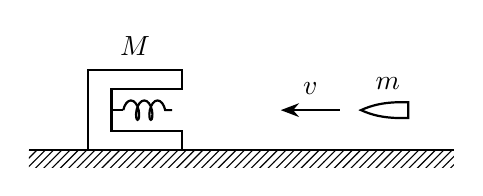
\begin{tikzpicture}[>=Stealth, thick]
  % Smooth horizontal floor with hatching
  \fill[pattern=north east lines] (0,-0.22) rectangle (5.4,0);
  \draw (0,0) -- (5.4,0);

  % Target block M with horizontal cavity open on the right
  \draw (0.75,0) -- (1.95,0) -- (1.95,0.24) -- (1.05,0.24)
    -- (1.05,0.78) -- (1.95,0.78) -- (1.95,1.02) -- (0.75,1.02) -- cycle;
  \node at (1.35,1.32) {$M$};

  % Coiled spring inside the cavity
  \draw (1.05,0.51) -- (1.20,0.51);
  \draw[decorate, decoration={coil, aspect=0.45, segment length=4.8pt, amplitude=3.5pt}]
    (1.20,0.51) -- (1.82,0.51);

  % Incoming bullet m moving left with velocity v
  \draw[->] (3.95,0.51) -- (3.20,0.51) node[midway, above=2pt] {$v$};
  \draw (4.82,0.41) -- (4.82,0.61)
    .. controls (4.52,0.62) and (4.35,0.57) .. (4.22,0.51)
    .. controls (4.35,0.45) and (4.52,0.40) .. (4.82,0.41) -- cycle;
  \node at (4.56,0.85) {$m$};
\end{tikzpicture}

\end{center}
\end{problem}
\clearpage


\begin{problem}{2.4.3}
一辆质量为 m 的车以速度 v 驶向另一辆原来静止的质量为 3m 的车，在两车正碰时弹簧被压缩，如图 2.79 所示.

(1) 若机械能是守恒的,那么在弹簧压缩最大的瞬间,质量为 3m 的那辆车的速度多大?

(2) 若机械能不守恒的话, 结果是否不一样?

(3) 若机械能守恒, 经过较长的一段时间后, 较重的车的末速度多大?

(4) 对于完全非弹性碰撞的情形,较重的车的末速度多大?
\begin{center}
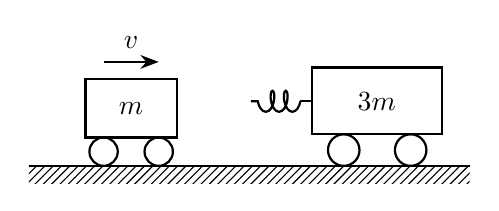
\begin{tikzpicture}[>=Stealth, thick]
  % Smooth horizontal floor with hatching
  \fill[pattern=north east lines] (0,-0.22) rectangle (5.6,0);
  \draw (0,0) -- (5.6,0);

  % Left cart of mass m
  \draw (0.95,0.18) circle (0.18);
  \draw (1.65,0.18) circle (0.18);
  \draw (0.72,0.36) rectangle (1.88,1.10);
  \node at (1.30,0.73) {$m$};
  \draw[->] (0.95,1.32) -- (1.65,1.32) node[midway, above=1pt] {$v$};

  % Right cart of mass 3m with attached spring
  \draw (4.00,0.20) circle (0.20);
  \draw (4.85,0.20) circle (0.20);
  \draw (3.60,0.40) rectangle (5.25,1.25);
  \node at (4.42,0.82) {$3m$};

  % Coiled spring on left side of 3m cart
  \draw (3.60,0.82) -- (3.45,0.82);
  \draw[decorate, decoration={coil, aspect=0.45, segment length=4.8pt, amplitude=3.8pt}]
    (3.45,0.82) -- (2.82,0.82);
\end{tikzpicture}

\end{center}
\end{problem}
\clearpage


\begin{problem}{2.4.6}
一质量为 $M$ 的车上装有一根杆，用一细绳将质量为 $\mu$ 的球挂在杆上 $P$ 点，车和球的初速度为 $v$ ，这辆车撞到另一辆质量为 $m$ 的原来静止的车上并且和它粘在一起.若细绳的长度为 $R$ ，试证明能使球绕 $P$ 点转圆圈的最小初速度为 $v = \left(\frac{m + M}{m}\right)\sqrt{5gR}$ ，忽

略摩擦并假定 $M, m \gg \mu.$
\begin{center}
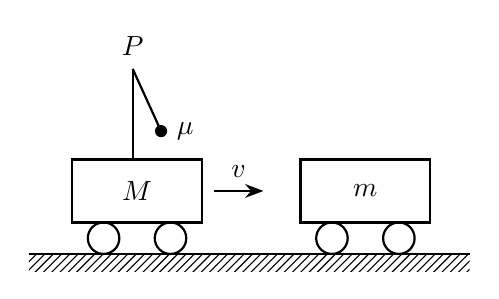
\begin{tikzpicture}[>=Stealth, thick]
  % Smooth horizontal floor with hatching
  \fill[pattern=north east lines] (0,-0.22) rectangle (5.6,0);
  \draw (0,0) -- (5.6,0);

  % Left cart of mass M with pole and pendulum
  \draw (0.95,0.20) circle (0.20);
  \draw (1.80,0.20) circle (0.20);
  \draw (0.55,0.40) rectangle (2.20,1.20);
  \node at (1.375,0.80) {$M$};

  % Vertical pole and pendulum bob mu
  \coordinate (P) at (1.32,2.35);
  \coordinate (Bob) at (1.68,1.56);
  \draw (1.32,1.20) -- (P);
  \node[above=1pt] at (P) {$P$};
  \draw (P) -- (Bob);
  \fill (Bob) circle (2.2pt) node[right=2pt] {$\mu$};

  % Velocity arrow v
  \draw[->] (2.35,0.80) -- (2.98,0.80) node[midway, above=1pt] {$v$};

  % Right stationary cart of mass m
  \draw (3.85,0.20) circle (0.20);
  \draw (4.70,0.20) circle (0.20);
  \draw (3.45,0.40) rectangle (5.10,1.20);
  \node at (4.275,0.80) {$m$};
\end{tikzpicture}

\end{center}
\end{problem}
\clearpage


\begin{problem}{2.4.7}
一弹子球从阶梯上弹下，在每一台阶都落在同一位置，都弹起相同的高度，每个台阶的高度和宽度相等为 $l$ ，每次碰撞恢复系数为 $\bm{e}$ .求弹子球所必需的水平速度 $\bm{v}_{h}$ 和每次弹起的高度 $H$
\end{problem}
\clearpage


\begin{problem}{2.4.8}
一质量为 m、荷电为 q、初速为 v 的粒子，和另一个处于静止的全同粒子发生正碰，求：

(1) 两个粒子最接近时的距离；

(2) 最接近的瞬时两个粒子的速度；

(3) 两个粒子的末速度.
\end{problem}
\clearpage


\begin{problem}{2.4.9}
小球 1 从离碗底高 h 处静止滑下,与静置于碗底的完全相同的小球 2 发生非

弹性碰撞,若恢复系数为 e,求第一次碰撞后两球达到的高度(忽略一切摩擦力).
\end{problem}
\clearpage


\begin{problem}{2.4.10}
质量为 $m_{1}$ 和 $m_{2}$ 的两个小球悬挂在长度分别为 $l_{1}$ 和 $l_{2}$ 的不可伸长的轻绳下，两球恰好相切。在两线所在的平面内把第一个小球拉到与铅垂线成 $\alpha$ 角的位置，静止后再放开，摆下与静止的第二个球发生弹性碰撞。求第一次碰撞后两球偏离铅垂线的最大角度 $\alpha_{1}$ 和 $\alpha_{2}$ 。
\end{problem}
\clearpage


\begin{problem}{2.4.11}
一个运动粒子与另一个静止的全同粒子发生弹性碰撞,试证明:碰后两粒子的运动方向相互垂直.
\end{problem}
\clearpage


\begin{problem}{2.4.12}
两个完全相同的光滑小球,一个静止,另一个以 $v_{0}$ 的速度与之发生非弹性碰撞.测得原静止的小球以 $\frac{3}{8}v_{0}$ 的速率向着偏离 $v_{0}$ 方向60°的方向运动.求:

(1) 恢复系数 e,

(2) 原来运动的小球的散射角.
\begin{center}
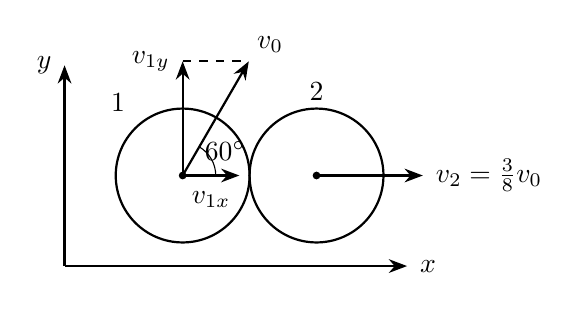
\begin{tikzpicture}[>=Stealth, thick]
  % Coordinate axes
  \coordinate (O) at (0,0);
  \draw[->] (O) -- (0,2.55) node[left=1pt] {$y$};
  \draw[->] (O) -- (4.35,0) node[right=1pt] {$x$};

  % Two identical touching spheres
  \coordinate (C1) at (1.50,1.15);
  \coordinate (C2) at (3.20,1.15);
  \draw (C1) circle (0.85);
  \draw (C2) circle (0.85);
  \fill (C1) circle (1.4pt);
  \fill (C2) circle (1.4pt);
  \node at (0.68,2.08) {$1$};
  \node at (3.20,2.22) {$2$};

  % Velocity components and initial velocity on sphere 1
  \coordinate (V1x) at (2.22,1.15);
  \coordinate (V1y) at (1.50,2.60);
  \coordinate (V0)  at (2.34,2.60);
  \draw[->] (C1) -- (V1x) node[midway, below=2pt] {$v_{1x}$};
  \draw[->] (C1) -- (V1y) node[left=1pt] {$v_{1y}$};
  \draw[->] (C1) -- (V0)  node[above right=-1pt] {$v_0$};
  \draw[dashed] (V1y) -- (V0);

  % 60 degree angle
  \pic[draw, thin, angle radius=0.42cm, angle eccentricity=1.48, "$60^\circ$"] {angle = V1x--C1--V0};

  % Velocity of sphere 2
  \draw[->] (C2) -- (4.55,1.15) node[right=1pt] {$v_2=\frac{3}{8}v_0$};
\end{tikzpicture}

\end{center}
\end{problem}
\clearpage


\begin{problem}{2.4.13}
一个质量为 $m_{1}$ 以 $\bm{v}_{10}$ 的速度运动的粒子1，与一个质量为 $m_{2}$ 的静止粒子2发生弹性斜碰撞，碰撞后，在质心平动参考系中，粒子1的散射角为 $\alpha_{\mathrm{c}}$ 。试证：在实验室参考系中两粒子的速度与 $\bm{v}_{10}$ 的夹角 $\alpha, \beta$ 满足下列关系：

\[
\tan \alpha = \frac {m _ {2} \sin \alpha_ {\mathrm{c}}}{m _ {1} + m _ {2} \cos \alpha_ {\mathrm{c}}}, \quad \tan \beta = \frac {\sin \alpha_ {\mathrm{c}}}{1 - \cos \alpha_ {\mathrm{c}}}
\]
\end{problem}
\clearpage


\begin{problem}{2.4.14}
一质量为 $m$ 的质子以 $v_{0}(v_{0} \ll c)$ 的速度去撞击静止的质量为 $4m$ 的氦核，用实验室参考系，质子以 $\frac{1}{2} v_{0}$ 的速率和 $30^{\circ}$ 的角度散射。求：

（1）用实验室参考系，撞击后氦核的速率及运动方向；

(2) 用质心平动参考系, 质子的散射速度.
\begin{center}
\begin{tikzpicture}[>=Stealth, thick]
  % Coordinate axes (x right, y down)
  \coordinate (O) at (0,1.45);
  \draw[->] (O) -- (1.05,1.45) node[right=1pt] {$x$};
  \draw[->] (O) -- (0,0.35) node[below=1pt] {$y$};

  % Proton (top) and its scattered velocity
  \coordinate (Cp) at (2.45,1.45);
  \draw (Cp) circle (0.30);
  \node at (1.92,1.88) {质子};
  \coordinate (Href) at (4.15,1.45);
  \coordinate (Vp) at ($(Cp) + (30:1.90)$);
  \draw[dashed] (Cp) -- (Href);
  \draw[->] (Cp) -- (Vp) node[above right=-1pt] {$\frac{1}{2}v_0$};
  \pic[draw, thin, angle radius=0.82cm, angle eccentricity=1.28, "$30^\circ$"] {angle = Href--Cp--Vp};

  % Helium nucleus (bottom) and its recoil velocity components
  \coordinate (Che) at (3.00,0.72);
  \draw (Che) circle (0.45);
  \node at (2.05,0.68) {氦核};
  \coordinate (V2x) at (4.50,0.72);
  \coordinate (V2y) at (3.00,-0.12);
  \coordinate (V2)  at (4.50,-0.12);
  \draw[->] (Che) -- (V2x) node[right=1pt] {$v_{2x}$};
  \draw[->] (Che) -- (V2y) node[below left=-1pt] {$v_{2y}$};
  \draw[->] (Che) -- (V2);
  \draw[dashed] (V2x) -- (V2) -- (V2y);
  \pic[draw, thin, angle radius=0.72cm, angle eccentricity=1.28, "$\alpha$"] {angle = V2--Che--V2x};
\end{tikzpicture}

\end{center}
\end{problem}
\clearpage


\chapter{振动和波}

\section{简谐振动}

\begin{problem}{3.1.1}
一平台在竖直方向做简谐振动, 振幅为 $5 \mathrm{~cm}$ , 频率为 $\frac{10}{\pi} \mathrm{s}^{-1}$ , 在平台到达最低点时, 将一木块轻轻地放在平台上 (设木块质量远小于平台质量. 问:

(1) 木块于何处离开平台？

(2) 木块能达到的高度比平台能达到的高度高多少?
\end{problem}
\clearpage


\begin{problem}{3.1.2}
图 3.1 中质量为 2kg 的物体从平衡位置拉开并释放后以 $\frac{\pi}{6}s$ 的周期在光滑的水平面上沿直线振动.

(1) 将它由平衡位置拉开 2cm 需要多大作

用力？

(2) 如果将一小质量块放在 2kg 质量块上, 它们之间的静摩擦因数为 0.1, 问: 2kg 物体的振动振幅不超过何值时, 小质量块对它无相对运动? (假定附加小质量块后对振动周期的影响可以忽略)
\begin{center}
\begin{tikzpicture}[>=Stealth, scale=1]
  % Hatched walls and floor
  \fill[pattern=north east lines] (-0.22, -0.22) rectangle (0, 1.35);
  \fill[pattern=north east lines] (0, -0.22) rectangle (5.2, 0);
  \fill[pattern=north east lines] (5.2, -0.22) rectangle (5.42, 1.35);
  \draw[thick] (0, 1.35) -- (0, 0) -- (5.2, 0) -- (5.2, 1.35);

  % Mass block
  \draw[thick, fill=white] (2.15, 0) rectangle (3.05, 0.90);
  \node at (2.60, 0.45) {$2\,\mathrm{kg}$};

  % Left and right springs
  \draw[thick, decorate, decoration={zigzag, segment length=5.5, amplitude=3.2, pre length=14, post length=14}] (0, 0.45) -- (2.15, 0.45);
  \draw[thick, decorate, decoration={zigzag, segment length=5.5, amplitude=3.2, pre length=14, post length=14}] (3.05, 0.45) -- (5.2, 0.45);
\end{tikzpicture}

\end{center}
\end{problem}
\clearpage


\begin{problem}{3.1.3}
在劲度系数为 $k$ 的弹簧下悬挂一质量为 $m$ 的盘子, 处于静止状态. 有一质量也为 $m$ 的物体, 自比原静止的盘子高 $h$ 处由静止落下, 与盘子做完全弹性碰撞 (碰撞时机械能不损失), 求:

(1) 头两次碰撞期间盘子的运动；

(2) 用作图法求第三次碰撞的时间(取第一次碰撞时 t=0).
\end{problem}
\clearpage


\begin{problem}{3.1.4}
两个完全相同的圆柱体, 它们的轴平行, 且在同一水平面上, 相距为 $2L$ , 以相同的角速率按图 3.3 所示方向绕轴快速转动, 在圆柱体上放一均质木板, 木板与圆柱体之间的滑动摩擦因数为 $\mu$ . 开始把木板放在平衡位置偏右 $x_0$ 的位置, 且给它一个向右的初速度 $v_0$ , 求木板的运动.
\begin{center}
\begin{tikzpicture}[>=Stealth, scale=1]
  % Two rotating cylinders
  \draw[thick] (-1.45, 0) circle (0.95);
  \draw[thick] (1.45, 0) circle (0.95);

  % Rotation arrows (left clockwise, right counterclockwise)
  \draw[->, thick] (-1.45, 0) ++(155:0.72) arc (155:100:0.72);
  \draw[->, thick] (1.45, 0) ++(25:0.72) arc (25:80:0.72);

  % Horizontal plank resting on top
  \draw[thick, fill=white] (-2.75, 0.95) rectangle (2.75, 1.13);

  % Distance 2L between cylinder axes
  \draw[thin] (-1.45, -1.08) -- (-1.45, -1.52);
  \draw[thin] (1.45, -1.08) -- (1.45, -1.52);
  \draw[<->, thin] (-1.45, -1.32) -- (1.45, -1.32) node[midway, above=2pt] {$2L$};
\end{tikzpicture}

\end{center}
\end{problem}
\clearpage


\begin{problem}{3.1.5}
质量为 $m$ 和 $2m$ 的两质点系在一个不可伸长的轻绳两端，并搭在光滑的滑轮上，在 $m$ 的下端用原长为 $a$ 、劲度系数 $k = \frac{mg}{a}$ 的质量可忽略的弹簧与另一个质量为 $m$ 的质点相连。

开始时从下列状态:三个质点均静止;绳被拉紧;弹簧为原长开始运动.求:

(1) 任何时刻两质量为 m 的质点间的距离；

(2) 绳子张力；

(3) 弹簧对质点的作用力.
\end{problem}
\clearpage


\begin{problem}{3.1.6}
一质点被一根轻弹性绳系于固定点 $A$ ，绳的固有长度为 $a$ ，当悬挂质点平衡后，绳的长度为 $a + b$ ，今质点从 $A$ 点静止下降，求质点落到最低点与 $A$ 点间的距离以及此过程所用的时间。
\end{problem}
\clearpage


\begin{problem}{3.1.7}
滑轮上绕有不可伸长的轻绳, 绳上悬一弹簧, 弹簧的另一端挂一质量为 $m$ 的物体, 当滑轮等角速度转动时, 物体以等速度 $v_{0}$ 下降, 此时弹簧伸长量为 $\lambda$ . 如将滑轮突然停住, 求此后运动中弹簧的最大伸长量和绳子的最大张力.
\begin{center}
\begin{tikzpicture}[>=Stealth, scale=1]
  % Pulley
  \draw[thick] (-0.72, 2.80) circle (0.72);

  % String and spring
  \draw[thick] (0, 2.80) -- (0, 2.25);
  \draw[thick, decorate, decoration={zigzag, segment length=5.5, amplitude=3.2}] (0, 2.25) -- (0, 1.15);
  \draw[thick] (0, 1.15) -- (0, 0.72);

  % Mass block and initial velocity
  \draw[thick, fill=white] (-0.42, 0.08) rectangle (0.42, 0.72);
  \node at (0, 0.40) {$m$};
  \draw[->, thick] (0, 0.08) -- (0, -0.58) node[below=1pt] {$v_0$};

  % Elongation lambda and t=0 mark
  \draw[thin] (-0.08, 1.15) -- (-0.82, 1.15);
  \draw[thin] (-0.42, 0.40) -- (-0.82, 0.40);
  \draw[<->, thin] (-0.64, 0.40) -- (-0.64, 1.15) node[midway, left=2pt] {$\lambda$};
  \node[anchor=north east] at (-0.46, 0.34) {$t=0\text{ 时}$};

  % Coordinate axis x
  \draw[thin] (0.72, 0.40) -- (1.12, 0.40) node[right=2pt] {$0$};
  \draw[->, thick] (0.92, 0.40) -- (0.92, -1.05) node[below=1pt] {$x$};
\end{tikzpicture}

\end{center}
\end{problem}
\clearpage


\begin{problem}{3.1.8}
如果通过实心的均质分布的无自转动的地球沿一条直径钻一小隧道，一块石头从地球的一边从静止开始让它掉入隧道，经 $t_{1}=\frac{\pi}{\omega_{0}}$ 时间后在地球的另一边会看到它。如果石头不是掉入而是以速度 $v_{0}$ 抛入，问 $v_{0}$ 应当多大才能使它经 $t_{2}=\frac{1}{2}t_{1}$ 时间后在地球的另一边出现？答案用 $\omega_{0}$ 和地球的半径R给出。
\end{problem}
\clearpage


\begin{problem}{3.1.9}
一根不计质量、不可伸长的绳子，穿过光滑的水平桌面上的小孔，两端分别连着质量分别为 $m_{1}$ 和 $m_{2}$ 的两个物体。 $m_{1}$ 在水平桌面上做半径为 $r_{0}$ 的圆周运动时， $m_{2}$ 静止不动，如图3.8所示。今给 $m_{2}$ 一个向下的极小的冲量，证明 $m_{2}$ 将做简谐振动，并求出其振动周期（小孔的摩擦力可忽略不计）。
\begin{center}
\begin{tikzpicture}[>=Stealth, scale=1]
  % Horizontal tabletop in perspective
  \draw[thick] (-2.4, -0.70) -- (1.6, -0.70) -- (2.4, 0.70) -- (-1.6, 0.70) -- cycle;

  % Dashed circular orbit
  \draw[dashed, thick] (0, 0) ellipse (1.25 and 0.46);

  % Strings and masses
  \coordinate (M1) at ({1.25*cos(28)}, {0.46*sin(28)});
  \draw[thick] (0, 0) -- (M1);
  \draw[thick] (0, 0) -- (0, -2.15);

  % Small hole at center
  \draw[thick, fill=white] (0, 0) circle (0.065);

  % Masses m1 and m2
  \fill (M1) circle (0.075) node[right=3pt] {$m_1$};
  \fill (0, -2.15) circle (0.075) node[right=3pt] {$m_2$};
\end{tikzpicture}

\end{center}
\end{problem}
\clearpage


\begin{problem}{3.1.10}
一质量为 $M$ 的质点在势能 $V(x) = -kxe^{-ax}(k$ 和 $a$ 均为正值、常量)的影响下沿 $x$ 轴运动, 求平衡位置和在此平衡位置附近做小幅振动的周期. 若 $k$ 和 (或) $a$ 是负的常数, 情况如何?
\end{problem}
\clearpage


\begin{problem}{3.1.11}
悬挂在原点的“单摆”，两边用旋轮线

\[
x = a (\varphi - \sin \varphi), y = a (1 - \cos \varphi)
\]

(其中 $\varphi$ 为产生旋轮线的半径为 a 的圆轮转过的角度)做成挡板来对“单摆”的摆长加以限制,如图所示.“单摆”由长度为 4a 的不可伸长的轻绳和摆锤构成.证明:

(1) 摆锤的轨迹是一条旋轮线；

(2) 摆锤的运动是周期运动, 其周期为 $T = 2\pi \sqrt{\frac{4a}{g}}$ , 与摆幅无关.

提示:用自然坐标的运动微分方程,证明 $\sin\theta$ 做简谐振动, $\theta$ 是摆线的直线部分与 y 轴的夹角.
\begin{center}
\begin{tikzpicture}[>=Stealth, scale=1]
  \def\a{0.44}

  % Coordinate axes
  \draw[->, thick] ({-2*pi*\a - 0.30}, 0) -- ({2*pi*\a + 0.35}, 0) node[below=2pt] {$x$};
  \draw[->, thick] (0, 0.42) -- (0, {-4*\a - 0.55}) node[right=2pt] {$y$};
  \node[above left=1pt] at (0, 0) {$O$};

  % Left and right cycloid barriers
  \draw[thick, domain=0:360, samples=72, smooth]
    plot ({-\a*(\x*pi/180 - sin(\x))}, {-\a*(1 - cos(\x))});
  \draw[thick, domain=0:360, samples=72, smooth]
    plot ({\a*(\x*pi/180 - sin(\x))}, {-\a*(1 - cos(\x))});

  % Bob trajectory (involute cycloid)
  \draw[dashed, thick, domain=-180:180, samples=72, smooth]
    plot ({\a*(\x*pi/180 + sin(\x))}, {-\a*(3 + cos(\x))});

  % Length 4a annotation
  \draw[thin] (-0.42, {-4*\a}) -- (0.12, {-4*\a});
  \draw[<->, thin] (-0.24, 0) -- (-0.24, {-4*\a}) node[pos=0.58, left=2pt, fill=white, inner sep=1pt] {$4a$};
\end{tikzpicture}

\end{center}
\end{problem}
\clearpage


\begin{problem}{3.1.12}
若放置在光滑的水平面上的弹簧振动系统,弹簧的质量不可忽略,证明系统的振动周期为

\[
T = 2 \pi \sqrt {\frac {M + m / 3}{k}}
\]

其中 m 为弹簧的质量, k 为弹簧的劲度系数, M 为系于弹簧上的物体的质量.

提示: 可将弹簧等效于一个弹簧振子: 质量可忽略的弹簧的原长和劲度系数均与质量不可忽略的弹簧一样, 连在弹簧上的物体质量为 $m'$ , 先证明 $m' = \frac{1}{3}m$ .
\end{problem}
\clearpage


\begin{problem}{3.1.13}
一个质量为 $m$ 的小物体放在光滑的水平面上被两个原长为 $l_0$ 、劲度系数为 $k$ 的弹簧约束，在图3.11所示的平衡位置附近做小振动。

(1)求小振动的角频率；

(2) 如果弹簧原长变为 $2l_{0}$ ，运动将会发生什么定性变化？
\begin{center}
\begin{tikzpicture}[>=Stealth, scale=1]
  % Hatched walls and floor
  \fill[pattern=north east lines] (-0.22, -0.22) rectangle (0, 1.35);
  \fill[pattern=north east lines] (0, -0.22) rectangle (5.2, 0);
  \fill[pattern=north east lines] (5.2, -0.22) rectangle (5.42, 1.35);
  \draw[thick] (0, 1.35) -- (0, 0) -- (5.2, 0) -- (5.2, 1.35);

  % Mass block
  \draw[thick, fill=white] (2.25, 0) rectangle (2.95, 0.85);
  \node[above=2pt] at (2.60, 0.85) {$m$};

  % Left and right springs
  \draw[thick, decorate, decoration={zigzag, segment length=5.5, amplitude=3.2, pre length=14, post length=14}] (0, 0.425) -- (2.25, 0.425);
  \draw[thick, decorate, decoration={zigzag, segment length=5.5, amplitude=3.2, pre length=14, post length=14}] (2.95, 0.425) -- (5.2, 0.425);
  \node at (1.125, 0.72) {$k$};
  \node at (4.075, 0.72) {$k$};

  % Dimension labels 2l_0
  \draw[thin] (0, -0.28) -- (0, -0.96);
  \draw[thin] (2.60, -0.28) -- (2.60, -0.96);
  \draw[thin] (5.2, -0.28) -- (5.2, -0.96);
  \draw[<->, thin] (0, -0.78) -- (2.60, -0.78) node[midway, above=2pt] {$2l_0$};
  \draw[<->, thin] (2.60, -0.78) -- (5.2, -0.78) node[midway, above=2pt] {$2l_0$};
\end{tikzpicture}

\end{center}
\end{problem}
\clearpage


\begin{problem}{3.1.14}
一个机器内某零件的振动规律为

\[
x = 0. 4 \sin \omega t + 0. 3 \cos \omega t
\]

x 的单位为 cm, $\omega = 20s^{-1}$ . 求这个振动的振幅、最大速度及最大加速度.

\[
x = A \cos (\omega t + \alpha) = A \cos \omega t \cos \alpha - A \sin \omega t \sin \alpha
\]

与 $x = 0.4\sin \omega t + 0.3\cos \omega t$ 比较，可得

\[
A \mathrm{cos} \alpha = 0. 3, \quad A \mathrm{sin} \alpha = - 0. 4
\]

解得

\[
A = \sqrt {(0 . 3) ^ {2} + (- 0 . 4) ^ {2}} = 0. 5 (\mathrm{cm})
\]

\[
v _ {\max} = A w = 0. 5 \times 2 0 = 1 0 (\mathrm{cm} \cdot \mathrm{s} ^ {- 1})
\]

\[
a _ {\max} = A w ^ {2} = 0. 5 \times (2 0) ^ {2} = 2 0 0 (\mathrm{cm} \cdot \mathrm{s} ^ {- 2})
\]
\end{problem}
\clearpage


\begin{problem}{3.1.15}
判断下列振动是否周期运动,若是周期运动,求出它的周期.

期 $T = \sqrt{2}\pi .$
\end{problem}
\clearpage


\begin{problem}{3.1.16}
两个在同一直线上做频率相同的简谐振动的合振动的振幅为 $10\mathrm{cm}$ , 合振动的相位超前第一个振动 $\frac{\pi}{6}$ , 第一个振动的振幅 $A_{1} = 8.0\mathrm{cm}$ . 求第二个振动的振幅 $A_{2}$ 及它与第一个振动的相位差.
\end{problem}
\clearpage


\begin{problem}{3.1.17}
一弹簧振子的劲度系数 $k_{1} = 9.8\mathrm{N}/$ $\mathbf{m}$ ，质量 $m = 9.8\times 10^{-2}\mathrm{kg}$ ，它的影子水平地投射在一屏上，该屏的质量 $M = 0.98\mathrm{kg}$ ，通过劲度系数 $k_{2}$ $= 98\mathrm{N / m}$ 的弹簧挂起来，如图3.13所示．开始时，把它们都从平衡位置拉下 $0.10\mathrm{m}$ ，先释放弹簧振子，如果要使影子在屏上振动的振幅为 $0.050\mathrm{m}$ ，问要过多长时间释放屏？并写出影子在屏上的振动方程.
\begin{center}
\begin{tikzpicture}[>=Stealth, scale=1]
  % Hatched ceiling
  \fill[pattern=north east lines] (-0.2, 3.2) rectangle (4.5, 3.42);
  \draw[thick] (-0.2, 3.2) -- (4.5, 3.2);

  % Left spring and mass m
  \draw[thick, decorate, decoration={zigzag, segment length=5.5, amplitude=3.2, pre length=14, post length=8}] (0.9, 3.2) -- (0.9, 1.51);
  \node[left=5pt] at (0.9, 2.35) {$k_1$};
  \draw[thick, fill=white] (0.9, 1.15) circle (0.36);
  \node[left=3pt] at (0.54, 1.15) {$m$};

  % Right spring and screen M
  \draw[thick, decorate, decoration={zigzag, segment length=5.5, amplitude=3.2, pre length=6, post length=6}] (3.25, 3.2) -- (3.25, 2.00);
  \node[right=5pt] at (3.25, 2.65) {$k_2$};
  \draw[thick, fill=white] (2.45, 2.25) -- (4.05, 1.75) -- (4.05, 0.05) -- (2.45, 0.55) -- cycle;
  \node at (3.65, 0.55) {$M$};

  % Horizontal projection onto screen
  \draw[dashed, thick] (0.9, 1.51) -- (3.25, 1.51);
  \draw[dashed, thick] (0.9, 0.79) -- (3.25, 0.79);
  \draw[dashed, thick] (3.25, 1.15) ellipse (0.14 and 0.36);
\end{tikzpicture}

\end{center}
\end{problem}
\clearpage


\begin{problem}{3.1.18}
用旋转矢量法证明，在同一直线上的 N 个简谐振动，它们有相同的振幅 $A_{0}$ 、相同的角频率 $\omega_{0}$ 、相位依次超前 $\delta$ ，即

\[
x _ {i} = A _ {0} \cos [ \omega t + (i - 1) \delta ] \quad (i = 1, 2, \dots , N)
\]

叠加后的合振动

\[
x = \sum_ {i = 1} ^ {N} x _ {i} = A _ {0} \frac {\sin \left(\frac {1}{2} N \delta\right)}{\sin \left(\frac {1}{2} \delta\right)} \cos \left[ \omega t + \frac {1}{2} (N - 1) \delta \right]
\]

提示:考虑 N 个振幅矢量都是一个圆上的弦,每个振幅矢量是正多边形的一条边.
\end{problem}
\clearpage


\begin{problem}{3.1.19}
有两支标有 $256\mathrm{Hz}$ 的音叉, 一支是标准的, 另一支是待校正的. 同时敲击两支音叉, 在半分钟内能听到 45 拍, 若在待校正的音叉上适当涂蜡, 从少逐渐增多, 在半分钟内听到的拍数先减少到听不见拍声, 而后又增多, 问待校正音叉原来的频率多大?
\end{problem}
\clearpage


\begin{problem}{3.1.20}
画出在互相垂直的两个方向振动的合成运动的轨道,并在图上标明运动方向.

\[
x = A \sin \omega t, y = B \sin \left(\omega t - \frac {\pi}{3}\right); \tag {1}
\]

(2) $x = A\sin \omega t, y = B\sin \left(2\omega t + \frac{5}{4}\pi\right)$ .
\end{problem}
\clearpage


\begin{problem}{3.1.21}
图 3.18 中的各图是在相互垂直的两个方向振动合成的利萨如图形: 已知水平方向的振动的角频率为 $\omega$ , 求竖直方向的振动的角频率.

(a)

(b)

(c)
\begin{center}
\begin{tikzpicture}[>=Stealth, scale=1]
  \draw[thick] (-1.55, -2.05) rectangle (1.55, 2.05);
  \draw[thick, domain=0:360, samples=240, smooth]
    plot ({1.55*sin(3*\x)}, {2.05*sin(\x + 15)});
\end{tikzpicture}

\end{center}
\begin{center}
\begin{tikzpicture}[>=Stealth, scale=1]
  \draw[thick] (-1.55, -2.05) rectangle (1.55, 2.05);
  \draw[thick, domain=0:180, samples=200, smooth]
    plot ({-1.55*cos(4*\x)}, {2.05*cos(3*\x)});
\end{tikzpicture}

\end{center}
\begin{center}
\begin{tikzpicture}[>=Stealth, scale=1]
  \draw[thick] (-1.55, -2.05) rectangle (1.55, 2.05);
  \draw[thick, domain=0:360, samples=240, smooth]
    plot ({1.55*sin(3*\x)}, {-2.05*cos(2*\x - 20)});
\end{tikzpicture}

\end{center}
\end{problem}
\clearpage


\begin{problem}{3.1.22}
在图 3.19 所示的示波器荧光屏上显示的利萨如图形中, 已知水平偏转讯号的频率为 $100\mathrm{Hz}$ , 若运行方向如图中箭头所示, 且 $t = 0$ 时位于 $S$ 点. 试写出水平偏转讯号和竖直偏转讯号的表示式, 并求出 $P, Q$ 两点的 $x$ 坐标.
\begin{center}
\begin{tikzpicture}[>=Stealth, line cap=round, line join=round]
  \def\A{2.0}
  \def\B{2.0}

  % Bounding rectangle
  \draw[thick] (-\A, -\B) rectangle (\A, \B);

  % Coordinate axes
  \draw[->, thick] (-\A, 0) -- (\A + 0.55, 0) node[below] {$x$};
  \draw[->, thick] (0, -\B) -- (0, \B + 0.55) node[left] {$y$};

  % Lissajous curve: x(t) = A cos(2t), y(t) = -B cos(3t) for t in [0, pi]
  \draw[thick,
    postaction={decorate},
    decoration={markings, mark=at position 0.21 with {\arrow{Stealth}}}
  ] plot[domain=0:3.14159265, samples=80, smooth]
    ({\A*cos(deg(2*\x))}, {-\B*cos(deg(3*\x))});

  % Key point labels
  \node[below right] at (\A, -\B) {$S$};
  \node[below right] at (0.5*\A, 0) {$P$};
  \node[below] at (-0.5*\A, \B - 0.08) {$Q$};

  % Dimension 2B (left)
  \draw (-\A - 0.15, \B) -- (-\A - 0.55, \B);
  \draw (-\A - 0.15, -\B) -- (-\A - 0.55, -\B);
  \draw[<->] (-\A - 0.35, -\B) -- (-\A - 0.35, \B)
    node[midway, left] {$2B$};

  % Dimension 2A (bottom)
  \draw (-\A, -\B - 0.15) -- (-\A, -\B - 0.55);
  \draw (\A, -\B - 0.15) -- (\A, -\B - 0.55);
  \draw[<->] (-\A, -\B - 0.35) -- (\A, -\B - 0.35)
    node[midway, below] {$2A$};
\end{tikzpicture}

\end{center}
\end{problem}
\clearpage


\begin{problem}{3.1.23}
上题中, 若 t=0 时位于 P 点, 写出水平、竖直两方向偏转讯号的表示式.
\end{problem}
\clearpage


\begin{problem}{3.1.24}
对图 3.20 所示的各周期运动进行谐波分析.

(a)

(b)

(c)
\begin{center}
\begin{tikzpicture}[>=Stealth, line cap=round, line join=round]
  \def\T{1.3}
  \def\A{1.4}

  % Axes
  \draw[->, thick] (-0.35, 0) -- (3.45*\T, 0) node[below] {$t$};
  \draw[->, thick] (0, -0.35) -- (0, \A + 0.55) node[left] {$x$};
  \node[below left] at (0, 0) {$O$};
  \node[left] at (0, \A) {$A$};

  % Sawtooth periods
  \foreach \k in {0, 1, 2} {
    \draw[thick] (\k*\T, 0) -- ({(\k+1)*\T}, \A);
    \draw[thick, dashed] ({(\k+1)*\T}, \A) -- ({(\k+1)*\T}, 0);
  }
  % Continuation after 3rd period
  \draw[thick] (3*\T, 0) -- (3.22*\T, 0.22*\A);

  % Period labels
  \node[below] at (\T, -0.05) {$\dfrac{2\pi}{\omega}$};
  \node[below] at (2*\T, -0.05) {$\dfrac{4\pi}{\omega}$};
  \node[below] at (3*\T, -0.05) {$\dfrac{6\pi}{\omega}$};
\end{tikzpicture}

\end{center}
\begin{center}
\begin{tikzpicture}[>=Stealth, line cap=round, line join=round]
  \def\qT{0.75} % quarter period pi/(2 omega)
  \def\A{1.05}

  % Axes
  \draw[->, thick] (-0.4, 0) -- (6.1*\qT, 0) node[below] {$t$};
  \draw[->, thick] (0, -\A - 0.35) -- (0, \A + 0.55) node[left] {$x$};
  \node[below left] at (0, 0) {$O$};
  \node[left] at (0, \A) {$A$};
  \node[left] at (0, -\A) {$-A$};

  % Square wave
  \draw[thick] (0, \A) -- (\qT, \A);
  \draw[thick, dashed] (\qT, \A) -- (\qT, -\A);
  \draw[thick] (\qT, -\A) -- (3*\qT, -\A);
  \draw[thick, dashed] (3*\qT, -\A) -- (3*\qT, \A);
  \draw[thick] (3*\qT, \A) -- (5*\qT, \A);
  \draw[thick, dashed] (5*\qT, \A) -- (5*\qT, -\A);
  \draw[thick] (5*\qT, -\A) -- (5.55*\qT, -\A);

  % Ticks and labels on t-axis
  \draw (2*\qT, 0) -- (2*\qT, 0.08);
  \node[below] at (2*\qT, -0.05) {$\dfrac{\pi}{\omega}$};
  \draw (4*\qT, 0) -- (4*\qT, 0.08);
  \node[below] at (4*\qT, -0.05) {$\dfrac{2\pi}{\omega}$};
\end{tikzpicture}

\end{center}
\begin{center}
\begin{tikzpicture}[>=Stealth, line cap=round, line join=round]
  \def\hT{0.82} % half period pi/omega
  \def\A{1.35}

  % Axes
  \draw[->, thick] (-0.35, 0) -- (5.7*\hT, 0) node[below] {$t$};
  \draw[->, thick] (0, -0.35) -- (0, \A + 0.55) node[left] {$x$};
  \node[below left] at (0, 0) {$O$};
  \node[left] at (0, \A) {$A$};

  % Triangle wave
  \draw[thick] (0, \A) -- (\hT, 0) -- (2*\hT, \A) -- (3*\hT, 0)
    -- (4*\hT, \A) -- (5*\hT, 0) -- (5.25*\hT, 0.25*\A);

  % Ticks and labels on t-axis
  \node[below] at (\hT, -0.05) {$\dfrac{\pi}{\omega}$};
  \draw (2*\hT, 0) -- (2*\hT, 0.07);
  \node[below] at (2*\hT, -0.05) {$\dfrac{2\pi}{\omega}$};
  \node[below] at (3*\hT, -0.05) {$\dfrac{3\pi}{\omega}$};
\end{tikzpicture}

\end{center}
\end{problem}
\clearpage


\section{阻尼振动和受迫振动}

\begin{problem}{3.2.1}
一质量为 $m$ 的质点在恢复力 $-kx$ 和阻力 $-r\dot{x}(k$ 和 $r$ 均为正的常量)的作用下运动, 其中 $x$ 是质点偏离平衡位置的位移. 对于固定的 $k$ 和一般的初始条件, $r = r_0$ 为何值时回到平衡位置所需的时间最短. 如果 $r > r_0$ , 是否可能对于特定的初始条件, 比 $r = r_0$ 能更快回到平衡位置? 如果 $r < r_0$ 呢?
\end{problem}
\clearpage


\begin{problem}{3.2.2}
如图 3.21 所示, 质量为 m=2000kg 的重物以 v=3cm/s 的速度匀速运动, 与质量可以忽略不计的弹簧及阻尼器相碰撞后一起做自由阻尼振动. 已知弹簧的劲度系数 k=48020N/m, 阻尼

器的阻尼系数 $\gamma = 1960\mathrm{N}\mathrm{s / m}$ ，问重物在碰撞后多少时间达到最大位移？最大位移多大？解沿 $v$ 的方向取 $x$ 轴，与阻尼器刚碰撞处取为 $x = 0$ ，此时 $t = 0$ 

\[
m \dot {x} = - k x - \gamma \dot {x}
\]

令 $\beta = \frac{\gamma}{2m},\omega_0^2 = \frac{k}{m}$ ，上式可改写为

\[
\dot {x} + 2 \beta \dot {x} + \omega_ {0} ^ {2} x = 0
\]

相应的特征方程为

\[
\begin{array}{r l} & r ^ {2} + 2 \beta r + \omega_ {0} ^ {2} = 0 \\ & r = - \beta \pm \sqrt {\beta^ {2} - \omega_ {0} ^ {2}} \\ & \omega_ {0} = \sqrt {\frac {k}{m}} = \sqrt {\frac {4 8 0 2 0}{2 0 0 0}} = 4. 9 \mathrm{s} ^ {- 1} \\ & \beta = \frac {\gamma}{2 m} = \frac {1 9 6 0}{2 \times 2 0 0 0} = 0. 4 9 \mathrm{s} ^ {- 1} \end{array}
\]

$\beta<\omega_{0}$ ，为弱阻尼情况，通解为

\[
x = A e ^ {- \beta t} \cos (\sqrt {\omega_ {0} ^ {2} - \beta^ {2}} t + \alpha)
\]

初始条件: t=0 时, x=0, $\dot{x}=v$ .

解得

\[
\begin{array}{r l} \dot {x} & = - \beta A \mathrm{e} ^ {- \beta t} \cos (\sqrt {\omega_ {0} ^ {2} - \beta^ {2}} t + \alpha) \\ & - A \sqrt {\omega_ {0} ^ {2} - \beta^ {2}} \mathrm{e} ^ {- \beta t} \sin (\sqrt {\omega_ {0} ^ {2} - \beta^ {2}} t + \alpha) \\ & A \cos \alpha = 0 \\ & - \beta A \cos \alpha - A \sqrt {\omega_ {0} ^ {2} - \beta^ {2}} \sin \alpha = v \\ & \alpha = - \frac {\pi}{2}, A = \frac {v}{\sqrt {\omega_ {0} ^ {2} - \beta^ {2}}} \end{array}
\]

\[
\begin{array}{c} x = \frac {v}{\sqrt {\omega_ {0} ^ {2} - \beta^ {2}}} \mathrm{e} ^ {- \beta t} \sin (\sqrt {\omega_ {0} ^ {2} - \beta^ {2}} t) \\ \dot {x} = - \frac {\beta v}{\sqrt {\omega_ {0} ^ {2} - \beta^ {2}}} \mathrm{e} ^ {- \beta t} \sin (\sqrt {\omega_ {0} ^ {2} - \beta^ {2}} t) + v \mathrm{e} ^ {- \beta t} \cos (\sqrt {\omega_ {0} ^ {2} - \beta^ {2}} t) \end{array}
\]

重物达到最大位移时， $\dot{x} = 0$ ，此时 $t = t_1$ 

\[
\begin{array}{r l} & {- \frac {\beta v}{\sqrt {\omega_ {0} ^ {2} - \beta^ {2}}} \sin (\sqrt {\omega_ {0} ^ {2} - \beta^ {2}} t _ {1}) + v \cos (\sqrt {\omega_ {0} ^ {2} - \beta^ {2}} t _ {1}) = 0} \\ & {\qquad t _ {1} = \frac {1}{\sqrt {\omega_ {0} ^ {2} - \beta^ {2}}} \arctan \left(\frac {\sqrt {\omega_ {0} ^ {2} - \beta^ {2}}}{\beta}\right) = 0. 3 0 \mathrm{s}} \end{array}
\]

最大位移为

\[
x \left(t _ {1}\right) = \frac {v}{\sqrt {\omega_ {0} ^ {2} - \beta^ {2}}} \mathrm{e} ^ {- \beta t _ {1}} \sin \left(\sqrt {\omega_ {0} ^ {2} - \beta^ {2}} t _ {1}\right) = 5. 2 8 \times 1 0 ^ {- 3} \mathrm{m}
\]
\begin{center}
\begin{tikzpicture}[>=Stealth, line cap=round, line join=round]
  % Left wall with hatching
  \fill[pattern=north east lines] (-0.25, 0.35) rectangle (0, 2.25);
  \draw[thick] (0, 0.35) -- (0, 2.25);

  % Horizontal ground with hatching
  \fill[pattern=north east lines] (0, -0.22) rectangle (5.6, 0);
  \draw[thick] (0, 0) -- (5.6, 0);

  % Dashpot (top)
  \draw[thick] (0, 1.65) -- (1.2, 1.65);
  \draw[thick] (1.2, 1.42) -- (1.2, 1.88);
  \draw[thick] (0.95, 1.98) -- (1.55, 1.98) -- (1.55, 1.32) -- (0.95, 1.32);
  \draw[thick] (1.55, 1.65) -- (1.92, 1.65);
  \node[above] at (1.25, 1.98) {$\gamma$};

  % Spring (bottom)
  \draw[thick] (0, 0.8) -- (0.5, 0.8);
  \draw[thick, decorate, decoration={zigzag, segment length=7pt, amplitude=3.5pt}]
    (0.5, 0.8) -- (1.5, 0.8);
  \draw[thick] (1.5, 0.8) -- (1.92, 0.8);
  \node[below] at (1.0, 0.62) {$k$};

  % Vertical bumper plate
  \draw[thick] (1.92, 0.35) rectangle (2.12, 2.05);

  % Velocity arrow
  \draw[->, thick] (3.55, 1.25) -- (2.8, 1.25) node[midway, above] {$v$};

  % Mass cart with wheels
  \draw[thick] (3.75, 0.42) rectangle (5.3, 1.65);
  \node at (4.525, 1.035) {$m$};
  \draw[thick] (4.1, 0.21) circle (0.21);
  \draw[thick] (4.95, 0.21) circle (0.21);
\end{tikzpicture}

\end{center}
\end{problem}
\clearpage


\begin{problem}{3.2.3}
一个有阻尼的弹簧振子系统, $m = 100\mathrm{kg}, k = 10000\mathrm{N / m}$ , 处于临界阻尼情况,由 $t = 0$ 时, $x_0 = 2.5\mathrm{cm}, \dot{x}_0 = -30\mathrm{cm / s}$ 开始运动. 问质量块将于几秒后到达平衡位置? 达到平衡位置后最远能移动多大距离?
\end{problem}
\clearpage


\begin{problem}{3.2.4}
如图 3.22 所示, 质量为 m 的薄板挂在弹簧的下端, 若空气的阻力可以不计,在空气中的振动周期为 $T_{1}$ ，在某液体中的振动周期为 $T_{2}$ ，液体的阻力可表示为 $-2\eta A v$ ，其中 A 为薄板的面积，v 为速度，

$\eta$ 为液体的黏度，试证 $\eta = \frac{2\pi m}{AT_1T_2}\cdot \sqrt{T_2^2 - T_1^2}.$
\begin{center}
\begin{tikzpicture}[>=Stealth, line cap=round, line join=round]
  % Ceiling
  \fill[pattern=north east lines] (-1.6, 3.6) rectangle (1.6, 3.85);
  \draw[thick] (-1.6, 3.6) -- (1.6, 3.6);

  % Spring and suspension rod
  \draw[thick] (0, 3.6) -- (0, 3.25);
  \draw[thick, decorate, decoration={zigzag, segment length=7pt, amplitude=3.5pt}]
    (0, 3.25) -- (0, 2.3);
  \node[right] at (0.12, 2.78) {$k$};
  \draw[thick] (0, 2.3) -- (0, 1.75);

  % Liquid surface
  \draw[thick] (-1.9, 2.2) -- (1.9, 2.2);

  % Liquid dashes (around plate)
  \foreach \x/\y in {-1.6/1.9, -1.0/1.85, 0.7/1.9, 1.4/1.85,
                     -1.5/1.45, -0.95/1.4, 1.05/1.45, 1.6/1.4,
                     -1.65/1.0, -1.05/0.95, 1.05/1.0, 1.6/0.95,
                     -1.5/0.55, -0.95/0.5, 1.1/0.55, 1.55/0.5,
                     -1.55/0.1, -0.85/0.05, 1.05/0.1, 1.55/0.05} {
    \draw[thick] (\x, \y) -- (\x + 0.22, \y);
  }

  % 3D thin rectangular plate (submerged)
  % Front face: (-0.5, 1.85), (0.55, 1.45), (0.55, 0.05), (-0.5, 0.45)
  % Back-top offset: (0.18, 0.1)
  \fill[white] (-0.5, 1.85) -- (0.55, 1.45) -- (0.55, 0.05) -- (-0.5, 0.45) -- cycle;
  \draw[thick] (-0.5, 1.85) -- (0.55, 1.45) -- (0.55, 0.05) -- (-0.5, 0.45) -- cycle;
  % Side and top thickness edges
  \draw[thick] (-0.5, 1.85) -- (-0.32, 1.95) -- (0.73, 1.55) -- (0.73, 0.15) -- (0.55, 0.05);
  \draw[thick] (0.55, 1.45) -- (0.73, 1.55);

  % Suspension rod visible down to attachment point on top face
  \draw[thick] (0, 2.2) -- (0, 1.71);

  % Labels on plate
  \node at (0.02, 1.30) {$m$};
  \node at (0.02, 0.78) {$A$};
\end{tikzpicture}

\end{center}
\end{problem}
\clearpage


\begin{problem}{3.2.5}
在图 3.23 所示系统中, 刚杆质量可忽略不计, 图中质量 m、弹簧的劲度系数 k、阻尼器阻尼系数 $\gamma$ 以及距离 a、b、l 均为已知. 写出运动微分方程. 由此求出做弱阻尼振动的角频率 $\omega_{d}$ 以及临界阻尼时 $\gamma = \gamma_{cr}$ 与其余各量间必须满足的关系.
\begin{center}
\begin{tikzpicture}[>=Stealth, line cap=round, line join=round]
  % Wall and pivot hinge at (0, 0)
  \fill[pattern=north east lines] (-0.42, -0.45) rectangle (-0.22, 0.45);
  \draw[thick] (-0.22, -0.45) -- (-0.22, 0.45);
  \draw[thick] (-0.22, 0.24) -- (0.0, 0.24) arc (90:-90:0.24) -- (-0.22, -0.24);
  \draw[thick] (0, 0) circle (0.06);

  % Rigid horizontal rod (from x=0.06 to x=4.68) and mass bob at x=4.95
  \draw[thick] (0.06, 0.07) -- (4.72, 0.07);
  \draw[thick] (0.06, -0.07) -- (4.72, -0.07);
  \draw[thick] (4.72, 0.07) arc (166:-166:0.25) -- cycle;
  \node[above right] at (4.95, 0.18) {$m$};

  % Dashpot at x = 1.9 (above rod)
  \fill[pattern=north east lines] (1.6, 1.75) rectangle (2.2, 1.95);
  \draw[thick] (1.6, 1.75) -- (2.2, 1.75);
  \draw[thick] (1.9, 1.75) -- (1.9, 1.15);
  \draw[thick] (1.72, 1.15) -- (2.08, 1.15);
  \draw[thick] (1.65, 1.35) -- (1.65, 0.85) -- (2.15, 0.85) -- (2.15, 1.35);
  \draw[thick] (1.9, 0.85) -- (1.9, 0.07);
  \node[right] at (2.18, 1.1) {$\gamma$};

  % Spring at x = 3.2 (below rod)
  \draw[thick] (3.2, -0.07) -- (3.2, -0.45);
  \draw[thick, decorate, decoration={zigzag, segment length=7pt, amplitude=3.5pt}]
    (3.2, -0.45) -- (3.2, -1.35);
  \draw[thick] (3.2, -1.35) -- (3.2, -1.75);
  \node[right] at (3.32, -0.9) {$k$};
  \fill[pattern=north east lines] (2.9, -1.95) rectangle (3.5, -1.75);
  \draw[thick] (2.9, -1.75) -- (3.5, -1.75);

  % Dimension extension lines
  \draw (0, -0.35) -- (0, -3.05);
  \draw (1.9, -0.2) -- (1.9, -1.0);
  \draw (3.2, -2.0) -- (3.2, -2.4);
  \draw (4.95, -0.35) -- (4.95, -3.05);

  % Dimension arrows a, b, l
  \draw[<->] (0, -0.75) -- (1.9, -0.75) node[midway, above] {$a$};
  \draw[<->] (0, -2.25) -- (3.2, -2.25) node[midway, above] {$b$};
  \draw[<->] (0, -2.88) -- (4.95, -2.88) node[midway, above] {$l$};
\end{tikzpicture}

\end{center}
\end{problem}
\clearpage


\begin{problem}{3.2.6}
质量为 0.2kg 的物体, 悬于劲度系数为 80N/m 的弹簧下, 此物体还受到阻力 $-\gamma v$ 的作用, v 是物体的速度. 若阻尼振动的频率为无阻尼振动频率的 $\frac{\sqrt{3}}{2}$ 倍, 阻尼系数 $\gamma$ 多大? 此系统 Q 值多大? 振动经 10 个整周后, 振幅减弱到原振幅的几分之几?
\end{problem}
\clearpage


\begin{problem}{3.2.7}
演奏钢琴上频率为 256Hz 的音键时, 1s 后振动能量减至初始值的一半. 问系统的 Q 值多大? 若高八度的音调(512Hz)也在 1s 后振动能量减至初始值的一半, 其 Q 值多大?
\end{problem}
\clearpage


\begin{problem}{3.2.8}
根据经典电磁理论,一个加速运动的电子在单位时间内辐射的能量为 $ke^{2}a^{2}/c^{3}$ , 其中 $k=6\times10^{9}Nm^{2}/C^{2}, e=1.60\times10^{-19}C$ (注意 k、e 的单位中的 C 是库仑, 勿与光速 c 混淆) $c=3.0\times10^{8}m/s, a$ 为电子的瞬时加速度.

(1) 若一电子沿一直线以频率 $\nu$ 及振幅 A 进行振荡, 假定每一周的运动可用 $x = A \cos(2\pi \nu t)$ 描述, 问在振荡一周的时间内, 它辐射了多少能量?

(2) 此振子之 Q 值多大?

(3) 在电子的运动的能量降至初始值的一半以前, 振荡已经历了多少个周期?
\end{problem}
\clearpage


\begin{problem}{3.2.9}
有一阻尼振子, 质量 $m = 0.2 \mathrm{~kg}, k = 80 \mathrm{~N} / \mathrm{m}, \gamma = 4 \mathrm{~N} \mathrm{~s} / \mathrm{m}$ , 受到强迫力 $F = F_{0} \cos \Omega t$ 作用, $F_{0} = 2 \mathrm{~N}, \Omega = 30 \mathrm{~s}^{-1}$ , 求:

(1) 稳态运动 $x = B \cos(\Omega t - \phi)$ 中的 B 和 $\phi$ ;

(2) 一周内反抗阻力耗散的机械能；

(3) 输入的平均功率.
\end{problem}
\clearpage


\begin{problem}{3.2.10}
如图 3.25 所示,作用于质量块上的强迫力 $F(t) = F_0\sin \Omega t$ , 弹簧支承端有运动, $x_s = a\cos \Omega t, \Omega \neq \sqrt{\frac{k}{m}}$ , $k$ 为弹簧的劲度系数, $m$ 为质量块的质量, 求稳态振动.
\begin{center}
\begin{tikzpicture}[>=Stealth, line cap=round, line join=round]
  % Left guide walls for sliding support
  \fill[pattern=north east lines] (0, 1.55) rectangle (1.15, 1.78);
  \draw[thick] (0, 1.55) -- (1.15, 1.55);
  \fill[pattern=north east lines] (0, 0.22) rectangle (1.15, 0.45);
  \draw[thick] (0, 0.45) -- (1.15, 0.45);

  % Sliding support block
  \draw[thick] (0.15, 0.52) rectangle (0.85, 1.48);

  % Spring
  \draw[thick] (0.85, 1.0) -- (1.25, 1.0);
  \draw[thick, decorate, decoration={zigzag, segment length=7pt, amplitude=3.5pt}]
    (1.25, 1.0) -- (2.45, 1.0);
  \draw[thick] (2.45, 1.0) -- (2.85, 1.0);
  \node[above] at (1.85, 1.18) {$k$};

  % Floor under cart
  \fill[pattern=north east lines] (2.2, -0.22) rectangle (4.65, 0);
  \draw[thick] (2.2, 0) -- (4.65, 0);

  % Mass cart with wheels
  \draw[thick] (2.85, 0.42) rectangle (4.15, 1.45);
  \node at (3.5, 0.935) {$m$};
  \draw[thick] (3.15, 0.21) circle (0.21);
  \draw[thick] (3.85, 0.21) circle (0.21);

  % Applied force F(t)
  \draw[->, thick] (4.15, 0.95) -- (5.2, 0.95) node[midway, above] {$F(t)$};

  % Coordinate axes below
  \draw[->, thick] (0.15, -0.65) -- (1.45, -0.65) node[below] {$x_s$};
  \node[below] at (0.15, -0.68) {$0$};

  \draw[->, thick] (2.25, -0.65) -- (5.2, -0.65) node[below] {$x$};
  \draw (2.85, -0.65) -- (2.85, -0.57);
  \node[below] at (2.85, -0.68) {$0$};
\end{tikzpicture}

\end{center}
\end{problem}
\clearpage


\begin{problem}{3.2.11}
图 3.28 所示的系统中, 弹簧悬点上下做简谐振动, $x_{s} = \frac{v_{0}}{\omega}\sin \omega t$ , 初始条件为 $x(0) = 0$ , $\dot{x}(0) = v_{0}$ , 弹簧的劲度系数为 $k$ , 质量块的质量为 $m$ , $\omega = \sqrt{\frac{k}{m}}$ . 求质量块的运动学方程.
\begin{center}
\begin{tikzpicture}[>=Stealth, line cap=round, line join=round]
  % Guide walls on left and right of sliding support
  \fill[pattern=north east lines] (-1.35, 3.0) rectangle (-0.45, 3.6);
  \draw[thick] (-1.35, 3.6) -- (-0.45, 3.6) -- (-0.45, 3.0) -- (-1.35, 3.0);

  \fill[pattern=north east lines] (0.45, 3.0) rectangle (1.35, 3.6);
  \draw[thick] (1.35, 3.6) -- (0.45, 3.6) -- (0.45, 3.0) -- (1.35, 3.0);

  % Sliding support block
  \draw[thick] (-0.38, 2.88) rectangle (0.38, 3.72);

  % Spring
  \draw[thick] (0, 2.88) -- (0, 2.38);
  \draw[thick, decorate, decoration={zigzag, segment length=7pt, amplitude=3.5pt}]
    (0, 2.38) -- (0, 1.38);
  \node[left] at (-0.15, 1.88) {$k$};
  \draw[thick] (0, 1.38) -- (0, 0.88);

  % Mass block
  \draw[thick] (-0.65, 0.25) rectangle (0.65, 0.88);
  \node[left] at (-0.72, 0.56) {$m$};

  % Coordinate axes on the right
  \draw[->, thick] (1.75, 3.72) -- (1.75, 2.35) node[right] {$x_s$};
  \node[right] at (1.78, 3.62) {$0$};

  \draw[->, thick] (0.95, 2.3) -- (0.95, -0.25) node[right] {$x$};
  \node[right] at (0.98, 2.2) {$0$};
\end{tikzpicture}

\end{center}
\end{problem}
\clearpage


\begin{problem}{3.2.12}
如图 3.29 所示, 单摆悬点沿水平方向做简谐振动, $x_{s}=a\sin\omega t$ , 已知摆长为 l, 摆锤质量为 m, 求微幅稳态振动中 $\theta$ 随时间的变化规律.
\begin{center}
\begin{tikzpicture}[>=Stealth, line cap=round, line join=round]
  % Horizontal sliding rod
  \draw[thick] (-2.6, 0) -- (2.6, 0);

  % Left bearing guide
  \draw[thick] (-2.2, 0.5) -- (-2.2, 0.1) -- (-1.35, 0.1) -- (-1.35, 0.5);
  \draw[thick] (-2.2, -0.5) -- (-2.2, -0.1) -- (-1.35, -0.1) -- (-1.35, -0.5);

  % Right bearing guide
  \draw[thick] (1.35, 0.5) -- (1.35, 0.1) -- (2.2, 0.1) -- (2.2, 0.5);
  \draw[thick] (1.35, -0.5) -- (1.35, -0.1) -- (2.2, -0.1) -- (2.2, -0.5);

  % Pivot coordinate x_s
  \draw[->, thick] (0, 0.35) -- (0.95, 0.35) node[above] {$x_s$};
  \node[above left] at (0.05, 0.35) {$0$};

  % Vertical dashed reference line
  \coordinate (O) at (0, 0);
  \coordinate (V) at (0, -2.9);
  \draw[thick, dashed] (O) -- (V);

  % Pendulum rod and bob (angle 24 deg from vertical)
  \def\L{2.55}
  \def\ang{24}
  \coordinate (M) at ({\L*sin(\ang)}, {-\L*cos(\ang)});
  \draw[thick] (O) -- node[midway, above right] {$l$} (M);
  \filldraw[fill=white, draw=black, thick] (M) circle (0.18);
  \node[right] at ($(M) + (0.2, 0)$) {$m$};

  % Angle theta
  \pic[draw, angle radius=0.85cm, angle eccentricity=1.35, "$\theta$"] {angle=V--O--M};
\end{tikzpicture}

\end{center}
\end{problem}
\clearpage


\begin{problem}{3.2.13}
图 3.30 所示系统中, 刚性杆 $AB$ 的质量可忽略不计, $B$ 端作用的强迫力 $F(t) = F_0 \sin \omega t$ , 图中 $m, k, \gamma, l$ 均为已知量。写出系统的运动微分方程, 并求下列情况下质量 $m$ 做上下稳态振动的振幅:

(1)系统发生共振；

(2) $\omega$ 等于固有频率 $\omega_0$ 的一半.
\begin{center}
\begin{tikzpicture}[>=Stealth, line width=0.7pt]
  % Left fixed wall and hinge A
  \fill[pattern=north east lines] (-0.65,-0.55) rectangle (-0.45,0.55);
  \draw[line width=0.9pt] (-0.45,-0.55) -- (-0.45,0.55);
  \draw (-0.45,0.22) -- (0,0.08);
  \draw (-0.45,-0.22) -- (0,-0.08);

  % Rigid massless bar AB
  \draw (0,0.08) -- (4.8,0.08) -- (4.8,-0.08) -- (0,-0.08) -- cycle;

  % Hinge circle A and mass m
  \draw[fill=white] (0,0) circle (0.11);
  \node[above=5pt] at (0,0.11) {$A$};
  \draw[fill=white] (1.6,0) circle (0.24);
  \node[above=2pt] at (1.6,0.24) {$m$};

  % Dashpot at x = 3.2
  \draw (3.2,-0.08) -- (3.2,-0.98);
  \draw (3.06,-0.98) -- (3.34,-0.98);
  \draw (2.98,-0.80) -- (2.98,-1.25) -- (3.42,-1.25) -- (3.42,-0.80);
  \draw (3.2,-1.25) -- (3.2,-1.75);
  \node[right=2pt] at (3.42,-1.02) {$\gamma$};
  \fill[pattern=north east lines] (2.8,-1.92) rectangle (3.6,-1.75);
  \draw[line width=0.9pt] (2.8,-1.75) -- (3.6,-1.75);

  % Force F(t) and label B at x = 4.8
  \draw[->] (4.8,0.08) -- (4.8,1.05) node[left=2pt, pos=0.85] {$F(t)$};
  \node[right=3pt] at (4.8,0) {$B$};

  % Spring k at x = 4.8
  \draw (4.8,-0.08) -- (4.8,-0.45);
  \draw[decorate, decoration={coil, aspect=0.4, segment length=4.5pt, amplitude=3.5pt}] (4.8,-0.45) -- (4.8,-1.40);
  \draw (4.8,-1.40) -- (4.8,-1.75);
  \node[right=4pt] at (4.8,-0.92) {$k$};
  \fill[pattern=north east lines] (4.4,-1.92) rectangle (5.2,-1.75);
  \draw[line width=0.9pt] (4.4,-1.75) -- (5.2,-1.75);

  % Bottom dimension lines (l, l, l)
  \foreach \x in {0, 1.6, 3.2, 4.8} {
    \draw[thin] (\x,-2.22) -- (\x,-2.65);
  }
  \draw[<->] (0,-2.48) -- (1.6,-2.48) node[midway, above=2pt] {$l$};
  \draw[<->] (1.6,-2.48) -- (3.2,-2.48) node[midway, above=2pt] {$l$};
  \draw[<->] (3.2,-2.48) -- (4.8,-2.48) node[midway, above=2pt] {$l$};
\end{tikzpicture}

\end{center}
\end{problem}
\clearpage


\begin{problem}{3.2.14}
图 3.31 中所有刚性杆质量均可忽略不计, m、k、 $\gamma$ 和 l 均为已知, 弹簧支承端有运动, $x_{s}=a\sin\omega t$ . 求系统的固有频率 $\omega_{0}$ 、阻尼比 $\zeta\left(=\frac{\beta}{\omega_{0}}\right)$ 及微幅稳态振动的振幅.
\begin{center}
\begin{tikzpicture}[>=Stealth, line width=0.7pt]
  % Top ceiling and hinge
  \fill[pattern=north east lines] (2.25,2.22) rectangle (3.15,2.39);
  \draw[line width=0.9pt] (2.25,2.22) -- (3.15,2.22);
  \draw (2.52,2.22) -- (2.63,1.80);
  \draw (2.88,2.22) -- (2.77,1.80);

  % L-shaped rigid massless bar
  \draw (2.62,1.80) -- (2.62,0.40) -- (2.78,0.40) -- (2.78,1.72) -- (5.40,1.72) -- (5.40,1.88) -- (2.62,1.88) -- cycle;

  % Hinge circle and mass m
  \draw[fill=white] (2.70,1.80) circle (0.11);
  \draw[fill=white] (5.40,1.80) circle (0.24);
  \node[above=2pt] at (5.40,2.04) {$m$};

  % Left guide slot and slider block
  \fill[pattern=north east lines] (-0.20,0.82) rectangle (0.65,0.98);
  \draw[line width=0.9pt] (-0.20,0.82) -- (0.65,0.82);
  \fill[pattern=north east lines] (-0.20,-0.18) rectangle (0.65,-0.02);
  \draw[line width=0.9pt] (-0.20,-0.02) -- (0.65,-0.02);
  \draw (0.04,0.08) rectangle (0.42,0.72);

  % Spring k between slider and vertical bar
  \draw (0.42,0.40) -- (1.02,0.40);
  \draw[decorate, decoration={coil, aspect=0.4, segment length=4.5pt, amplitude=3.5pt}] (1.02,0.40) -- (1.88,0.40);
  \draw (1.88,0.40) -- (2.62,0.40);
  \node[above=4pt] at (1.45,0.40) {$k$};

  % Dashpot gamma to the right wall
  \draw (2.78,0.40) -- (3.85,0.40);
  \draw (3.85,0.26) -- (3.85,0.54);
  \draw (3.65,0.18) -- (4.10,0.18) -- (4.10,0.62) -- (3.65,0.62);
  \draw (4.10,0.40) -- (5.05,0.40);
  \node[below=3pt] at (3.92,0.18) {$\gamma$};
  \fill[pattern=north east lines] (5.05,0.05) rectangle (5.22,0.75);
  \draw[line width=0.9pt] (5.05,0.05) -- (5.05,0.75);

  % Dimension l (vertical)
  \draw[thin] (2.15,1.80) -- (2.56,1.80);
  \draw[<->] (2.28,0.40) -- (2.28,1.80) node[midway, left=2pt] {$l$};

  % Dimension 2l (horizontal)
  \draw[thin] (5.40,1.52) -- (5.40,1.15);
  \draw[<->] (2.78,1.32) -- (5.40,1.32) node[midway, above=2pt] {$2l$};

  % Coordinate axis x_s at bottom left
  \draw[->] (-0.25,-0.55) -- (1.40,-0.55);
  \node[below=2pt] at (-0.25,-0.55) {$O$};
  \node[below=2pt] at (1.30,-0.55) {$x_s$};
\end{tikzpicture}

\end{center}
\end{problem}
\clearpage


\begin{problem}{3.2.15}
一个无阻尼的弹簧振子的受迫振动, 若强迫力的角频率 $\Omega = 5\mathrm{s}^{-1}$ 时发生共振, 给质量块增加 $1\mathrm{kg}$ 的质量, 当 $\Omega = 4.8\mathrm{s}^{-1}$ 时发生共振. 求弹簧振子原来的质量块的质量及弹簧的劲度系数.
\end{problem}
\clearpage


\begin{problem}{3.2.16}
如图 3.32 所示,一台自由运行的马达,为了减少其振动被放置在一块薄的橡皮垫上,马达埋入橡皮垫 10cm. 估算马达出现最大竖直振动时的转速(每分钟转数).
\begin{center}
\begin{tikzpicture}[>=Stealth, line width=0.7pt]
  % Rubber pad depression and hatching
  \fill[pattern=north east lines]
    (-2.05,0.42) .. controls (-1.60,0.62) and (-1.15,0.35) .. (-0.92,0)
    -- (0.92,0)
    .. controls (1.15,0.35) and (1.60,0.62) .. (2.05,0.42)
    -- (2.05,-0.25) -- (-2.05,-0.25) -- cycle;
  \draw[line width=0.8pt]
    (-2.05,0.42) .. controls (-1.60,0.62) and (-1.15,0.35) .. (-0.92,0)
    -- (0.92,0)
    .. controls (1.15,0.35) and (1.60,0.62) .. (2.05,0.42);

  % Motor pedestal and concentric circles
  \draw (-0.75,0) -- (-0.54,0.66);
  \draw (0.75,0) -- (0.54,0.66);
  \draw[fill=white] (0,1.42) circle (0.95);
  \draw (0,1.42) circle (0.48);

  % 10cm depth dimension on the right
  \draw[thin] (1.02,0) -- (2.55,0);
  \draw[thin] (1.72,0.50) -- (2.55,0.50);
  \draw[<->] (2.36,0) -- (2.36,0.50);
  \node[right=2pt, rotate=90, anchor=north] at (2.42,0.25) {$10\,\mathrm{cm}$};
\end{tikzpicture}

\end{center}
\end{problem}
\clearpage


\begin{problem}{3.2.17}
如图 3.33 所示, 一辆汽车沿 x 方向行驶并保持不变的水平速度 v, 汽车经过一个隆起部分, 其形状为

\[
y _ {0} = A \left(1 - \cos \frac {\pi x}{l}\right)
\]

$(0 \leqslant x \leqslant 2l)$ , 其他地方 $y_0 = 0$ . 求汽车在经过隆起部分时在竖直方向的运动. 将汽车简化为一个质量为 $m$ 的质点放在一个原长为 $l_0$ 、劲度系数为 $k$ 的弹簧上。忽略一切阻力并假定弹簧始终保持竖直。
\begin{center}
\begin{tikzpicture}[>=Stealth, line width=0.7pt]
  % Axes
  \draw[->] (-0.6,0) -- (5.1,0) node[below=2pt] {$x$};
  \draw[->] (0,-0.4) -- (0,2.2) node[left=2pt] {$y$};
  \node[below left=1pt] at (0,0) {$O$};

  % Bump curve: y0 = A(1 - cos(pi x / l)) on [0, 2l], with l = 2.1, A = 0.5
  \draw[line width=0.8pt] plot[domain=0:4.2, samples=80] (\x, {0.5*(1 - cos(deg(pi*\x/2.1)))});

  % Dashed vertical line at x = l and axis labels
  \draw[dashed] (2.1,0) -- (2.1,1.0);
  \node[below=2pt] at (2.1,0) {$l$};
  \node[below=2pt] at (4.2,0) {$2l$};

  % Left snapshot of mass-spring system
  \draw (0.30,0.02) -- (0.30,0.20);
  \draw[decorate, decoration={coil, aspect=0.4, segment length=3.2pt, amplitude=2.5pt}] (0.30,0.20) -- (0.30,0.68);
  \draw (0.30,0.68) -- (0.30,0.80);
  \draw[fill=white] (0.14,0.80) rectangle (0.46,1.02);
  \node[above=1pt] at (0.30,1.02) {$m$};
  \draw[->] (0.46,0.44) -- (0.95,0.44) node[right=1pt] {$v$};

  % Middle snapshot of mass-spring system
  \pgfmathsetmacro{\ymid}{0.5*(1 - cos(deg(pi*1.45/2.1)))}
  \draw (1.45,\ymid) -- (1.45,\ymid+0.18);
  \draw[decorate, decoration={coil, aspect=0.4, segment length=3.2pt, amplitude=2.5pt}] (1.45,\ymid+0.18) -- (1.45,\ymid+0.66);
  \draw (1.45,\ymid+0.66) -- (1.45,\ymid+0.78);
  \draw[fill=white] (1.29,\ymid+0.78) rectangle (1.61,\ymid+1.00);
  \draw[->] (1.61,\ymid+0.42) -- (2.10,\ymid+0.42) node[right=1pt] {$v$};
\end{tikzpicture}

\end{center}
\end{problem}
\clearpage


\begin{problem}{3.2.18}
一个由凸轮激励的、有阻尼的弹簧振子，如图3.34所示，凸轮使顶杆 $A$ 在铅垂方向按锯齿波规律做周期性运动，凸轮的升程为 $h$ ，周期为 $T$ ，顶杆又通过劲度系数为 $k_{1}$ 的弹簧使有阻尼的弹簧振子振动．弹簧振子的弹簧的劲度系数为 $k$ ，质量块质量为 $m$ ，阻尼系数为 $\gamma$ .求质量块的稳态振动.
\begin{center}
\begin{tikzpicture}[>=Stealth, line width=0.7pt]
  % Axes
  \draw[->] (0,0) -- (5.0,0) node[below=2pt] {$t$};
  \draw[->] (0,0) -- (0,2.1) node[left=2pt] {$y$};
  \node[below left=1pt] at (0,0) {$O$};

  % Tick for h
  \draw (0,1.4) -- (0.10,1.4);
  \node[left=2pt] at (0,1.4) {$h$};

  % Three sawtooth periods (T = 1.45)
  \draw[line width=0.8pt] (0,0) -- (1.45,1.4);
  \draw[dashed] (1.45,1.4) -- (1.45,0);
  \draw[line width=0.8pt] (1.45,0) -- (2.90,1.4);
  \draw[dashed] (2.90,1.4) -- (2.90,0);
  \draw[line width=0.8pt] (2.90,0) -- (4.35,1.4);
  \draw[dashed] (4.35,1.4) -- (4.35,0);

  % Period labels
  \node[below=2pt] at (1.45,0) {$T$};
  \node[below=2pt] at (2.90,0) {$2T$};
  \node[below=2pt] at (4.35,0) {$3T$};
\end{tikzpicture}

\end{center}
\begin{center}
\begin{tikzpicture}[>=Stealth, line width=0.7pt]
  % Top fixed support
  \fill[pattern=north east lines] (-1.25,4.85) rectangle (1.25,5.03);
  \draw[line width=0.9pt] (-1.25,4.85) -- (1.25,4.85);

  % Left branch: dashpot gamma
  \draw (-0.55,4.85) -- (-0.55,4.35);
  \draw (-0.77,3.90) -- (-0.77,4.35) -- (-0.33,4.35) -- (-0.33,3.90);
  \draw (-0.69,4.10) -- (-0.41,4.10);
  \draw (-0.55,4.10) -- (-0.55,3.30);
  \node[left=3pt] at (-0.77,4.12) {$\gamma$};

  % Right branch: spring k
  \draw (0.55,4.85) -- (0.55,4.52);
  \draw[decorate, decoration={coil, aspect=0.4, segment length=4.2pt, amplitude=3.5pt}] (0.55,4.52) -- (0.55,3.62);
  \draw (0.55,3.62) -- (0.55,3.30);
  \node[right=4pt] at (0.55,4.07) {$k$};

  % Mass block m
  \draw (-1.20,2.75) rectangle (1.20,3.30);
  \node at (0,3.025) {$m$};

  % Lower spring k1
  \draw (0,2.75) -- (0,2.38);
  \draw[decorate, decoration={coil, aspect=0.4, segment length=4.2pt, amplitude=3.5pt}] (0,2.38) -- (0,1.48);
  \draw (0,1.48) -- (0,1.18);
  \node[right=4pt] at (0,1.93) {$k_1$};

  % Guide walls and pushrod A
  \fill[pattern=north east lines] (-0.82,0.32) rectangle (-0.34,1.25);
  \draw (-0.82,1.25) -- (-0.34,1.25) -- (-0.34,0.32) -- (-0.82,0.32);
  \fill[pattern=north east lines] (0.34,0.32) rectangle (0.82,1.25);
  \draw (0.82,1.25) -- (0.34,1.25) -- (0.34,0.32) -- (0.82,0.32);
  \draw (-0.22,0.30) rectangle (0.22,1.18);
  \node at (0,0.74) {$A$};

  % Cam profile below pushrod A
  \draw[line width=0.8pt]
    (0,-0.80)
    .. controls (-0.65,-0.80) and (-0.72,-0.15) .. (-0.30,0.16)
    .. controls (-0.05,0.34) and (0.38,0.22) .. (0.62,0.02)
    .. controls (0.72,-0.07) and (0.52,-0.12) .. (0.45,-0.25)
    .. controls (0.40,-0.55) and (0.30,-0.80) .. (0,-0.80);

  % Cam pivot and fixed base
  \fill[pattern=north east lines] (-0.34,-0.62) rectangle (0.34,-0.50);
  \draw (-0.34,-0.50) -- (0.34,-0.50);
  \draw (-0.18,-0.50) -- (-0.06,-0.26);
  \draw (0.18,-0.50) -- (0.06,-0.26);
  \draw[fill=white] (0,-0.22) circle (0.08);

  % Rotation arrow on the left of cam
  \draw[->] (-0.78,-0.05) to[bend right=30] (-0.78,-0.75);
\end{tikzpicture}

\end{center}
\end{problem}
\clearpage


\begin{problem}{3.2.19}
(1)一个有阻尼的受迫谐振子,它的运动微分方程为

\[
m \ddot {x} = - m \omega_ {0} ^ {2} x - \gamma \dot {x} + A \cos \omega t
\]

它的平均能量损耗率多大？

(2) 一个非谐振子的运动微分方程为

\[
m \ddot {x} = - m \omega_ {0} ^ {2} x + \alpha x ^ {2} + A \cos \omega t
\]

其中 $\alpha$ 为一个小的常量, t=0 时, x=0, $\dot{x}=0$ , 求此后的运动到 $\alpha$ 的一次项.
\end{problem}
\clearpage


\begin{problem}{3.2.20}
无阻尼的非线性自由振动,质量为 m 的振子受力

\[
F (x) = - k x + m \lambda x ^ {2}
\]

其中 $\lambda$ 是小常量，求振子满足初始条件 t=0 时 $x(0)=A,\dot{x}(0)=0$ 的一级和二级近似解.
\end{problem}
\clearpage


\begin{problem}{3.2.21}
已知一个单摆的悬挂点做强迫竖直小振动 $\eta(t)=\eta_{0}\cos\omega t$ ，此单摆由长为 L 的无质量杆和杆端的质点组成。

(1) 假设单摆摆角振幅很小, $\eta_{0}\ll L$ ,求摆角 $\varphi$ 满足的运动微分方程;

(2) 求满足初始条件 t=0 时 $\varphi=a,\dot{\varphi}=0$ 的一级近似解；

(3) $w$ 为何值时发生共振, 写出共振时满足式(2)给的初始条件的一级近似解.
\end{problem}
\clearpage


\section{简谐波}

\begin{problem}{3.3.1}
一平面简谐波

\[
y = 0. 2 \sin [ \pi (0. 5 x - 3 0 t) ]
\]

x、y 的单位为厘米，t 的单位为秒．求波的振幅、波长、频率、波速以及 x=1cm 处质元振动的初相位．
\end{problem}
\clearpage


\begin{problem}{3.3.2}
一波的频率为 $20s^{-1}$ ，波速为 $80m \cdot s^{-1}$ ，振幅为 0.02m，求：

(1) 波的相位相差 $45^{\circ}$ 的两个点间的距离；

(2) 在一给定点处, 时间相隔 0.01s 的两位移之相位差;

(3) 在一给定点处, 时间相隔 0.01s 的质元的两个位置的最大距离;

(4) 在一给定点处, 质元的振动相位相差 $45^{\circ}$ 的质元的两个位置的最大距离.
\end{problem}
\clearpage


\begin{problem}{3.3.3}
一列沿长弦线向 $x$ 正方向传播的平面简谐波，位于 $x = x_{1} = 0$ 及 $x = x_{2} = 1\mathrm{m}$ 处两质元的简谐振动如下：

\[
y _ {1} = 0. 2 \sin 3 \pi t, y _ {2} = 0. 2 \sin \left(3 \pi t + \frac {\pi}{8}\right)
\]

$y$ 的单位为米， $t$ 的单位为秒．求：

(1) 频率；

(2) 波长 $\lambda;$ 

(3) 波速 v;

(4) 该两质元的相对速率的最大值.
\begin{center}
\begin{tikzpicture}[>=Stealth, line width=0.7pt]
  \def\L{4.5}
  \def\ang{22.5}
  \coordinate (O) at (0,0);
  \coordinate (A) at ({\L*cos(\ang)},{\L*sin(\ang)});
  \coordinate (B) at ({\L*cos(\ang)-\L},{\L*sin(\ang)});

  % Horizontal reference line
  \draw (O) -- (\L,0);

  % Vectors
  \draw[->, line width=0.8pt] (O) -- (A) node[midway, below right=2pt] {$0.6\pi$};
  \draw[->, line width=0.8pt] (A) -- (B) node[midway, above=2pt] {$0.6\pi$};
  \draw[->, line width=0.8pt] (O) -- (B) node[midway, left=3pt] {$|\dot{y}_2 - \dot{y}_1|_{\max}$};

  % Angle labels
  \node at (1.95,0.34) {$\dfrac{\pi}{8}$};
  \node at (2.45,1.35) {$\dfrac{\pi}{8}$};
\end{tikzpicture}

\end{center}
\end{problem}
\clearpage


\begin{problem}{3.3.4}
一平面简谐波以 $50\mathrm{m / s}$ 的速率沿 $x$ 负方向传播，在 $t = 1\mathrm{s}$ 时的波形如图3.37所示，写出此波的运动学方程，并画出 $t = 1\mathrm{s}$ 时各质元的 $\frac{\partial y}{\partial t} - x$ 图.
\begin{center}
\begin{tikzpicture}[>=Stealth, line width=0.7pt]
  % Axes
  \draw[->] (0,0) -- (5.3,0);
  \node[below=2pt] at (5.1,-0.05) {\shortstack{$x$\\[-2pt](m)}};
  \draw[->] (0,-1.55) -- (0,1.75);
  \node[left=2pt] at (-0.02,1.55) {\shortstack{$y$\\[-2pt](mm)}};

  % Wave curve: y(x) = 1.05 * sin(360 * x / 5.0 + 30)
  % Zero crossings at x = 2.0833 and x = 4.5833 (half-wavelength = 2.5 cm -> 10 m)
  \draw[line width=0.85pt] plot[domain=0:4.85, samples=100] (\x, {1.05*sin(360*\x/5.0 + 30)});

  % Dashed extrema lines and y-axis labels
  \draw[dashed] (0,1.05) -- (0.833,1.05);
  \draw[dashed] (0,-1.05) -- (3.333,-1.05);
  \node[left=2pt] at (0,1.05) {$10$};
  \node[left=2pt] at (0,0.525) {$5$};
  \node[left=2pt] at (0,0) {$0$};
  \node[left=2pt] at (0,-1.05) {$-10$};

  % Half-wavelength dimension 10
  \draw[thin] (2.0833,0.06) -- (2.0833,1.05);
  \draw[thin] (4.5833,0.06) -- (4.5833,1.05);
  \draw[<->] (2.0833,0.84) -- (4.5833,0.84) node[midway, above=2pt] {$10$};
\end{tikzpicture}

\end{center}
\end{problem}
\clearpage


\begin{problem}{3.3.5}
一根均匀的长弦线, 线密度为 0.02kg/m, 被 50N 的力拉紧, 弦线的一端 x=0

做简谐振动, 振幅为 0.02m, 周期为 1s, t=0 时, 位移 y 为 0.01m, $\frac{\partial y}{\partial t}$ 为负值. 写出向 x 正方向传播的简谐波的运动学方程.
\end{problem}
\clearpage


\begin{problem}{3.3.6}
一脉冲从长弦线的一端行进至另一端,需时0.1秒,弦线跨过一滑轮后悬一质量为弦线质量100倍的重物,问弦线的长度多大?
\end{problem}
\clearpage


\begin{problem}{3.3.7}
在拉紧的弦线上传播一个脉冲：

\[
y (x, t) = \frac {b ^ {3}}{b ^ {2} + (a x + u t) ^ {2}}
\]

其中 $a, b, u$ 均为正值常量，问：

(1) 此介质是色散介质吗？说明理由；

(2) 该脉冲速率多大？方向如何？

(3) 弦线上 x=0 处质元在 t=1 时的振动速度.
\end{problem}
\clearpage


\begin{problem}{3.3.8}
在两端固定、长度为 100m 的弦线上,有一如图 3.39 所示的脉冲以 40m/s 的速率向右行进,且保持其形状不变.

(1) 定性地画出在脉冲处于图示位置时弦线各质元的振动速度的轮廓图；

(2) 近似地估算弦线质元的最大振动速度；

(3) 若弦线总质量为 2kg, 弦线中的张力有多大?
\begin{center}
\begin{tikzpicture}[>=Stealth, line width=0.7pt]
  % Left and right fixed walls
  \fill[pattern=north east lines] (-0.16,-0.32) rectangle (0,0.32);
  \draw[line width=0.8pt] (0,-0.32) -- (0,0.32);
  \fill[pattern=north east lines] (6.00,-0.32) rectangle (6.16,0.32);
  \draw[line width=0.8pt] (6.00,-0.32) -- (6.00,0.32);

  % String baseline and triangular pulse
  \draw[line width=0.8pt] (0,0) -- (6.00,0);
  \draw[line width=0.8pt] (1.95,0) -- (2.40,0.36) -- (2.85,0);

  % Top dimensions (40m, 60m)
  \draw[thin] (0,0.52) -- (0,0.98);
  \draw[thin] (2.40,0.52) -- (2.40,0.98);
  \draw[thin] (6.00,0.52) -- (6.00,0.98);
  \draw[<->] (0,0.80) -- (2.40,0.80) node[midway, above=2pt] {$40\,\mathrm{m}$};
  \draw[<->] (2.40,0.80) -- (6.00,0.80) node[midway, above=2pt] {$60\,\mathrm{m}$};

  % Pulse height dimension (0.1m)
  \draw[thin] (2.82,0.36) -- (3.22,0.36);
  \draw[<->] (3.06,0) -- (3.06,0.36);
  \node[right=2pt] at (3.06,0.18) {$0.1\,\mathrm{m}$};

  % Pulse half-width dimensions (1m, 1m)
  \draw[thin] (1.95,-0.12) -- (1.95,-0.62);
  \draw[thin] (2.40,-0.12) -- (2.40,-0.62);
  \draw[thin] (2.85,-0.12) -- (2.85,-0.62);
  \draw[<->] (1.95,-0.46) -- (2.40,-0.46) node[midway, above=1pt] {$1\,\mathrm{m}$};
  \draw[<->] (2.40,-0.46) -- (2.85,-0.46) node[midway, above=1pt] {$1\,\mathrm{m}$};
\end{tikzpicture}

\end{center}
\end{problem}
\clearpage


\begin{problem}{3.3.9}
一个对称的三角形脉冲在弦线上沿 $x$ 正方向运动, 其最大高度为 $0.4 \mathrm{~m}$ , 全长为 $1.0 \mathrm{~m}$ , 波速为 $24 \mathrm{~m} / \mathrm{s}$ , 在 $t = 0$ 时, 整个脉冲位于 $x = 0$ 至 $x = 1 \mathrm{~m}$ 之间. 画出 $x = 1 \mathrm{~m}$ 处质元振动速度随时间变化的曲线.
\end{problem}
\clearpage


\begin{problem}{3.3.10}
气体或液体的压缩系数定义为 $k = -\frac{1}{\gamma} \frac{\mathrm{d}V}{\mathrm{d}p}$ , 这里 $-\mathrm{d}V$ 是压强增加 $\mathrm{d}p$ 时的体积减小量, 标准状态下空气的压缩系数比水约大 15000 倍.

(1) 推导声波速度公式 $v=\frac{1}{\sqrt{k\rho}}$ ，其中 $\rho$ 是质量

密度；

(2) 在标准状态下, 空气中的声速约为 $330 \mathrm{~m} / \mathrm{s}$ , 水中的声速约为 $1470 \mathrm{~m} / \mathrm{s}$ , 假设水是充满了微小气泡的混合物, 微小气泡仅占总体积的 $1 \%$ (忽略由气泡引起的混合物的密度和纯水的密度之间的差异), 求混合物的压缩系数 $k$ , 再求混合物中的声速 $v$ 值, 并与纯水或空气中的声速 $v$ 值相比较.
\end{problem}
\clearpage


\begin{problem}{3.3.11}
(1) 写出在弦中传播基波的频率与弦的物理性质、几何性质的关系；

(2) 从牛顿运动定律出发, 分析一小段弦所发生的变化导出上述关系.
\end{problem}
\clearpage


\begin{problem}{3.3.12}
声音在气体中的速度由下式计算: $v = \sqrt{\text{绝热体积模量/密度}}$ .

(1) 证明此公式的量纲是对的；

(2) 此公式隐含着认为声音在空气中的传播是准静态过程,但从另一方面,在空气分子的方均根速率大致为 500m/s 的温度下,空气中的声速大致为 340m/s,那么这种过程为什么能够是准静态的?
\end{problem}
\clearpage


\begin{problem}{3.3.13}
若有下述两列波在介质中传播：

\[
y _ {1} = A \sin (5 x - 1 0 t), y _ {2} = A \sin (4 x - 9 t)
\]

式中 x、y 以米为单位，t 以秒为单位。

(1) 写出合成波的方程；

(2) 求群速度 $v_{g}$ ;

(3) 求出合成波中振幅为零的两相邻点间的距离；

(4) 说明此介质是否是色散介质,说明理由.
\end{problem}
\clearpage


\begin{problem}{3.3.14}
两个不同的音叉在完全相同的两段长绳上产生稳定的简谐波, 振幅 $A_{1} = 2A_{2}$ , 波长 $\lambda_{1} = \frac{1}{2}\lambda_{2}$ . 设绳子除了与音叉交换能量外, 不与其他物体交换能量. 求两音叉给予绳子的平均功率之比.
\end{problem}
\clearpage


\begin{problem}{3.3.15}
一正弦式空气波沿直径为 0.14m 的圆柱形管子的轴向传播, 波的强度为 $9.0 \times 10^{-3} J/m^{2} \cdot s$ , 频率为 300Hz, 波速为 300m/s, 求:

(1) 波中平均能量密度和最大能量密度；

(2) 每两个相邻质元同振动相位面间的区域中含有的机械能.
\end{problem}
\clearpage


\begin{problem}{3.3.16}
一波源以 $3.5 \times 10^{4} \mathrm{~W}$ 的功率发射球面电磁波，在某处测得该波的平均能量密度为 $7.8 \times 10^{-15} \mathrm{~J} / \mathrm{m}^{3}$ . 求该处离波源的距离. 电磁波的传播速度为 $3.0 \times 10^{8} \mathrm{~m} / \mathrm{s}$ .
\end{problem}
\clearpage


\begin{problem}{3.3.17}
两列平面简谐波

\[
\begin{array}{r l} & y _ {1} = A _ {1} \cos \left[ \omega_ {1} \left(t - \frac {x}{v}\right) + \alpha_ {1} \right] \\ & y _ {2} = A _ {2} \cos \left[ \omega_ {2} \left(t - \frac {x}{v}\right) + \alpha_ {2} \right] \end{array}
\]

同时在同一介质中传播,分别讨论 $\omega_{1}\neq\omega_{2}$ 及 $\omega_{1}=\omega_{2}$ 两种情况下波强是否等于两波分别单独传播时的波强之和.
\end{problem}
\clearpage


\section{边界效应和干涉}

\begin{problem}{3.4.1}
设反射波的振动方向仍保持入射波的振动方向, 若介质的杨氏模量值为切变模量值的 3 倍, 试用惠更斯原理求出一列纵波的反射波是一列横波的入射角以及一列在入射面内振动的横波的反射波为一列纵波的入射角, (不考虑这样的入射波、反射波能否遵从波的叠加原理的问题).
\end{problem}
\clearpage


\begin{problem}{3.4.2}
有一稀奇的现象,当风从声源向观察者吹时,人们偶而听到来自远方的声音,惊人的清楚.

(1) 说明这个现象不能用“随风而来”来解释, 即均匀的风速不能说明这个现象;

(2) 吹遍地面的风, 有一垂直的速度梯度, 在地面附近可近似表示为 $v = ky^2$ , 这里 $y$ 是离地面的高度, $k$ 是常数. 对于给定的 $k$ 值和声速 $v_{s}$ , 计算顺风时出现声强最大增强处离声源的距离 $s$ ;

提示: 可以假定声波线遵循下列轨道: $y = h \sin \frac{\pi x}{s}$ .

（3）人们还注意到，甚至在无风时，声音在湖面上传播也有增强现象。在这种情况下，将发生什么？
\end{problem}
\clearpage


\begin{problem}{3.4.3}
当平面简谐波垂直入射于两种介质的界面时,证明:对于没有耗散和吸收的无色散介质,在任何时刻,入射波的波强等于反射波的波强和透射波的波强之和.
\end{problem}
\clearpage


\begin{problem}{3.4.4}
两根连在一起的弦线, 线密度分别为 $\eta_{1}$ 和 $\eta_{2}$ , 设想有一波从弦线 2 向弦线 1 传播, 设入射波方程为

\[
y _ {2} = A \cos (\omega t - k _ {2} x) \quad (x <   0)
\]

边界位于 $x = 0$ 处．试分别求出 $\frac{\eta_2}{\eta_1} = \frac{1}{4}$ 和 $\frac{\eta_2}{\eta_1} = 9$ 时的反射波、透射波的数学表达式.
\end{problem}
\clearpage


\begin{problem}{3.4.5}
一列波从线密度为 $\eta_{1}$ 的弦线传向线密度为 $\eta_{2}$ 的弦线，在连接点处反射波和透射波振幅之比 $r$ 、相位关系与 $\eta_{1}, \eta_{2}$ 间有何关系？
\end{problem}
\clearpage


\begin{problem}{3.4.6}
平面声波自空气中垂直入射到水面上, 求振幅反射系数 $\frac{B}{A}$ 和振幅透射系数 $\frac{C}{A}$ 

提示:空气和水的体积弹性模量不同,在界面处, $\frac{\partial(y_{1}+y'_{1})}{\partial x}=\frac{\partial y_{2}}{\partial x}$ 的边界条件需作修改.
\end{problem}
\clearpage


\begin{problem}{3.4.7}
一长列振幅为 $A$ 的波包, 主要由角频率很接近 $\omega_0$ 的波组成, 它在一根无限长的线密度为 $\eta$ 、张力为 $T$ 的弦上传播. 波包碰到弦上一个质量为 $m$ 的小珠, 设 $mg \ll T$ .

(1) 求透射波振幅；

(2) 在 $m, \omega_{0}$ 很大的极限下，透射波振幅与 $\omega_{0}$ 有何关系？
\begin{center}
\begin{tikzpicture}[>=Stealth, line width=0.7pt]
  % Horizontal string before and after wave packet
  \draw[line width=0.8pt] (0,0) -- (0.45,0);
  \draw[line width=0.8pt] plot[domain=0.45:2.61, samples=120] (\x, {0.26*sin(360*(\x-0.45)/0.72)});
  \draw[line width=0.8pt] (2.61,0) -- (5.50,0);

  % Bead of mass m
  \fill (4.10,0) circle (0.075);
  \node[above=3pt] at (4.10,0.06) {$m$};

  % Peak-to-peak amplitude 2A
  \draw[thin] (0.63,0.26) -- (1.03,0.26);
  \draw[thin] (0.63,-0.26) -- (1.03,-0.26);
  \draw[<->] (0.83,-0.26) -- (0.83,0.26);
  \draw[thin] (0.83,0) -- (1.38,0.52) node[above right=-2pt] {$2A$};
\end{tikzpicture}

\end{center}
\end{problem}
\clearpage


\begin{problem}{3.4.8}
一列简谐波沿线密度为 $\eta$ 、张力为 $T_0$ 的弦线从右入射，被套在竖直棒上的无质量小环反射，如图3.51所示，环受到的摩擦力的大小与速率成正比，比例系数为 $\gamma$ 。求振幅的反射系数 $\frac{B}{A}$ ，并讨论 $\gamma \to \infty$ 和 $\gamma \to 0$ 的两极限情况。
\begin{center}
\begin{tikzpicture}[>=Stealth]
  % Axes
  \draw[->] (-0.1, 0) -- (4.8, 0) node[below] {$x$};
  \draw[->] (0, -0.75) -- (0, 1.45) node[left] {$y$};
  \node[below left] at (0, 0) {$O$};

  % Wave profile and massless ring at x = 0
  \draw[thick, smooth] plot[domain=0:4.35, samples=80] (\x, {0.62*sin(deg(1.45*\x + 0.45))});
  \fill (0, {0.62*sin(deg(0.45))}) circle (1.8pt);
\end{tikzpicture}

\end{center}
\end{problem}
\clearpage


\begin{problem}{3.4.9}
若上题的小环具有质量 $m$ ，环与竖直棒间无摩擦，有一列角频率为 $\omega$ 的简谐波被小环反射，求振幅的反射系数 $\frac{B}{A}$ 及与入射波的相位差。（设 $mg \ll T_0$ ）.
\end{problem}
\clearpage


\begin{problem}{3.4.10}
线密度为 $\eta$ 的一根长弦处在张力 $T_{0}$ 下，一点质量 m 附着在弦上某一点，从

左边入射一角频率为 $\omega$ 的波沿这弦传播，设 $mg \ll T_{0}$ .

(1) 计算被点质量 m 反射的那部分能量与入射能量之比；

(2) 假定点质量 $m$ 被一线密度为 $\eta' (\gg \eta)$ 、长度 $l = \frac{m}{\eta'}$ 的短弦代替，固定 $m$ 值不变，变 $l$ 和 $\eta', l$ 满足什么条件，上述结果能近似成立？
\end{problem}
\clearpage


\begin{problem}{3.4.11}
一个点质量 $m$ 附在线密度为 $\eta$ 、张力为 $T$ 的无限长的弦上，同时和一个劲度系数为 $k$ 的弹簧相连，并受到一个外加的力 $F(t)$ ，如图3.52所示。点质量运动时，它在弦上产生一个起始波。

(1)求质点的运动微分方程和弦的运动方程；

(2) 若 $F(t)=F_{0}\cos\omega t$ ，求辐射到弦上的平均功率（不考虑瞬变过程）；

(3) 如果没有驱动力, 点质量的振动将衰减掉, 证明它与弦耦合引起的阻尼等同于一个摩擦阻力 $f = -\gamma v$ , 其中 $v$ 是点质量的速度, 求 $\gamma$ 与弦的参数之间的关系.
\begin{center}
\begin{tikzpicture}[>=Stealth]
  % Fixed ceiling with hatching
  \draw[thick] (-0.65, 2.15) -- (0.65, 2.15);
  \foreach \x in {-0.55, -0.35, -0.15, 0.05, 0.25, 0.45} {
    \draw (\x, 2.15) -- (\x+0.15, 2.32);
  }

  % Axes and external force F(t)
  \draw[->] (-2.7, 0) -- (2.8, 0) node[below] {$x$};
  \draw[->] (0, 2.15) -- (0, 2.65) node[left] {$y$};
  \draw[->, thick] (0, -0.85) -- (0, 0.22);
  \node[right=2pt] at (0, -0.45) {$F(t)$};
  \node[below left] at (0, 0) {$O$};

  % Spring and point mass m
  \draw[decorate, decoration={zigzag, segment length=5.5pt, amplitude=3pt, pre length=12pt, post length=12pt}]
    (0, 2.15) -- (0, 0.30);
  \node[right=4pt] at (0, 1.25) {$k$};
  \fill (0, 0.30) circle (2pt) node[above right=1pt] {$m$};

  % Symmetric wave along the string
  \draw[thick] (0, 0.30)
    .. controls (0.35, 0.16) and (0.70, 0.16) .. (1.05, 0.40)
    .. controls (1.35, 0.62) and (1.65, 0.66) .. (2.00, 0.56)
    .. controls (2.30, 0.46) and (2.48, 0.32) .. (2.60, 0.20);
  \draw[thick] (0, 0.30)
    .. controls (-0.35, 0.16) and (-0.70, 0.16) .. (-1.05, 0.40)
    .. controls (-1.35, 0.62) and (-1.65, 0.66) .. (-2.00, 0.56)
    .. controls (-2.30, 0.46) and (-2.48, 0.32) .. (-2.60, 0.20);

  % Transverse displacement markers y_1 and y_2
  \draw[dashed] (-1.60, 0) -- (-1.60, 0.63);
  \node[right=1pt] at (-1.60, 0.30) {$y_1$};
  \draw[dashed] (1.60, 0) -- (1.60, 0.63);
  \node[right=1pt] at (1.60, 0.30) {$y_2$};
\end{tikzpicture}

\end{center}
\end{problem}
\clearpage


\begin{problem}{3.4.12}
由劲度系数为 $k$ 、原长为 $a$ 的非常多相同的弹簧连结的非常长的珠子链，如图3.53所示，每个珠子沿 $x$ 方向做无阻尼振动，除一个珠子质量为 $m_0$ 外，其余的质量均为 $m (> m_0)$ ，不计弹簧质量。

(1)求在远离那个特殊的珠子处传播的波的波矢和角频率之间的关系；

(2) 当一个波矢为 k 的波碰到这个特殊珠子时, 反射概率多大?
\begin{center}
\begin{tikzpicture}[>=Stealth]
  % Broken spring ends for infinite chain
  \draw[decorate, decoration={zigzag, segment length=3pt, amplitude=1.8pt}] (-2.85, 0) -- (-2.48, 0);
  \draw[decorate, decoration={zigzag, segment length=3pt, amplitude=1.8pt}] (2.48, 0) -- (2.85, 0);

  % Springs between masses
  \foreach \i in {-4, -3, -2, 1, 2, 3} {
    \draw[decorate, decoration={zigzag, segment length=3pt, amplitude=1.8pt, pre length=2pt, post length=2pt}]
      (\i*0.62 + 0.055, 0) -- (\i*0.62 + 0.62 - 0.055, 0);
    \node[above=5pt] at (\i*0.62 + 0.31, 0) {\small $K$};
  }
  \draw[decorate, decoration={zigzag, segment length=3pt, amplitude=1.8pt, pre length=2pt, post length=2pt}]
    (-0.62 + 0.055, 0) -- (-0.13, 0);
  \node[above=5pt] at (-0.31, 0) {\small $K$};
  \draw[decorate, decoration={zigzag, segment length=3pt, amplitude=1.8pt, pre length=2pt, post length=2pt}]
    (0.13, 0) -- (0.62 - 0.055, 0);
  \node[above=5pt] at (0.31, 0) {\small $K$};

  % Identical beads m
  \foreach \i in {-4, -3, -2, -1, 1, 2, 3, 4} {
    \fill (\i*0.62, 0) circle (1.8pt) node[below=3pt] {$m$};
    \node[above=14pt] at (\i*0.62, 0) {\small $\i$};
  }

  % Special mass m_0 at index 0
  \draw[fill=white, thick] (-0.13, -0.13) rectangle (0.13, 0.13);
  \node[below=5pt] at (0, -0.10) {$m_0$};
  \node[above=14pt] at (0, 0) {\small $0$};

  % x-direction arrow
  \draw[->] (1.65, -0.48) -- (2.90, -0.48) node[below] {$x$};
\end{tikzpicture}

\end{center}
\end{problem}
\clearpage


\begin{problem}{3.4.13}
一质量为 $m$ 、原长为 $l$ 的弹簧, 其劲度系数为 $k$ . 弹簧的一端固定, 另一端系一质量为 $M$ 的物体, 水平放置. $M$ 在光滑的水平面上运动.

(1) 导出该系统纵向振动的波动方程；

(2) 求出作为 $m$ 的函数的最小简正频率。这里 $M$ 和 $k$ 都是有限的，且 $m \ll M$ 。
\end{problem}
\clearpage


\begin{problem}{3.4.14}
一根无限长的细绳, 线密度为 $\eta$ , 张力为 $T$ . 在 $t = 0$ 时, 绳偏离平衡位置的位移为 $f(x)$ . 初始速度为 $g(x)$ , 求 $t > 0$ 时绳子的运动.
\end{problem}
\clearpage


\begin{problem}{3.4.15}
一根线密度为 $\eta$ 、张力为 $T$ 的绳， $x = 0$ 端固定， $x = l$ 端终止在一个不计质量的环上，环能在一垂直棒上无摩擦自由滑动、写 $x = l$ 端的边界条件，并求振动的简正模。
\end{problem}
\clearpage


\begin{problem}{3.4.16}
若上题环的质量为 $m$ ，求振动的简正模，并证明： $m \to \infty$ 时，简正模趋于两端固定的情况。
\end{problem}
\clearpage


\begin{problem}{3.4.17}
两种线密度的弦线在 $x = 0$ 处连接， $x > 0$ 处， $\eta = \eta_{2}, x < 0$ 处， $\eta = \eta_{1}$ ，张力为 $T$ 。一列简谐波从弦线1入射到连接点。分别 $\eta_{1} > \eta_{2}$ 和 $\eta_{1} < \eta_{2}$ 两种情况，讨论反射波、透

\[
\begin{array}{r l} M \frac {\mathrm{d} ^ {2} y _ {n}}{\mathrm{d} t ^ {2}} & = T \left(\frac {y _ {n + 1} - y _ {n}}{a}\right) - T \left(\frac {y _ {n} - y _ {n - 1}}{a}\right) \\ & = \frac {T}{a} (y _ {n + 1} - 2 y _ {n} + y _ {n - 1}) \quad n = 1, 2, \dots , N \end{array}
\]

其中 $y_0 = y_{n + 1} = 0$ 

由于 $N$ 相当大, 要用第十章求少自由度的小振动的简正模式的办法, 解 $N \times N$ 的行列式是困难的. 可用求解3.4.12的办法.

在同一振动模式中,各珠子有同样的角频率,相位

相同或相反,振幅不同,其解可写成

\[
y _ {n} = A _ {n} \cos (\omega t + \varphi) \quad n = 1, 2, \dots , N
\]

参照两端固定的弦的振动模式是各种驻波,对此珠子链,试用

\[
A _ {n} = A \sin k n a + B \cos k n a \quad n = 0, 1, \dots , N + 1
\]

由边界条件 $A_0 = 0$ 得 $B = 0$ ，故

\[
A _ {n} = A \sin k n a
\]

$A_{N + 1} = 0, \sin k(N + 1)a = 0$ ，即 $\sin kL = 0$ 

\[
k _ {m} l = m \pi ,
\]

\[
k _ {m} = \frac {m \pi}{L}, m = 1, 2, \dots , N
\]

将

$y_{n} = A\sin knacos(\omega t + \varphi)$ 代入方程组，得

\[
M \omega^ {2} \sin k n a = \frac {T}{a} [ \sin k (n + 1) a - 2 \sin k n a + \sin k (n - 1) a ]
\]

用三角公式 $\sin \alpha +\sin \beta = 2\sin \frac{\alpha + \beta}{2}\cos \frac{\alpha - \beta}{2}$ 

上式化为

\[
- M \omega^ {2} = \frac {2 T}{a} (\cos k a - 1)
\]

故

\[
\omega_ {m} ^ {2} = \frac {2 T}{M a} \left(1 - \cos \frac {m \pi a}{L}\right) m = 1, 2, \dots , N
\]

作几点附带说明：

\[
1) y _ {n} = A \sin k _ {m} n a \cos (\omega_ {m} t + \varphi_ {m})
\]

用 $\sin \alpha \cos \beta = \frac{1}{2} [\sin (\alpha +\beta) + \sin (\alpha -\beta)]$ 可改写为

\[
y _ {n} = \frac {1}{2} A \left[ \sin \left(k _ {m} n a + \omega_ {m} t + \varphi_ {m}\right) + \sin \left(k _ {m} n a - \omega_ {m} t - \varphi_ {m}\right) \right]
\]

第一项表示向左边传播的波,第二项表示向右边传播的波.

波的传播速度有两种计算方法:考虑向右传播的波

\[
\sin (k _ {m} n a - \omega_ {m} t - \varphi_ {n})
\]

考虑相邻的两个珠子的振动在紧挨的处于同相位的两个时刻

\[
\begin{array}{r l} k _ {m} n a - \omega_ {m} t _ {1} - \varphi_ {m} & = k _ {m} (n + 1) a - \omega_ {m} t _ {2} - \varphi_ {m} \\ v _ {m} & = \frac {a}{t _ {2} - t _ {1}} = \frac {\omega_ {m}}{k _ {m}} \end{array}
\]

令 $\omega_{m}^{2} = \frac{2T}{Ma} (1 - \cos k_{m}a),\frac{\omega_{m}}{k_{m}}\neq$ 常量(对于不同的 $\omega_{m}$ ).说明对于不同角频率的振动，其相

位的传播速度是不同的.

波速的另一种计算方法是把 $y_{n}$ 改成 $y(x)$ 的形式： $\sin (k_m n a - \omega_m t - \varphi_m)$ 改成 $\sin (k_m x - \omega_m t - \varphi_m) = -\sin \left[\omega_m \left(t - \frac{k_m}{\omega_m} x\right) + \varphi_m\right]$ ，即可看出 $v_m = \frac{\omega_m}{k_m}$ .

2) 考虑连续的极限情况．保持 L 不变，令 $N \to \infty, a \to 0, \frac{M}{a} = \eta$ 

\[
\begin{array}{r l}\omega_ {m} ^ {2}&= \frac {2 T}{M a} (1 - \cos k _ {m} a) = \frac {4 T}{M a} \sin^ {2} \frac {1}{2} k _ {m} a\\&= \frac {4 T}{M a} \cdot \left(\frac {1}{2} k _ {m} a\right) ^ {2} \left(\frac {\sin \frac {1}{2} k _ {m} a}{\frac {1}{2} k _ {m} a}\right) ^ {2}\\&\rightarrow \frac {4 T}{M a} \cdot \frac {1}{4} k _ {m} a ^ {2} = \frac {T}{\eta} k _ {m} ^ {2} = \frac {T}{\eta} \frac {m ^ {2} \pi^ {2}}{L ^ {2}}\\&\omega_ {m} \rightarrow \frac {m \pi}{L} \sqrt {\frac {T}{\eta}}\end{array}
\]

与两端固定的连续弦的情况完全相同.

3)对于有 N 个珠子的珠子链, $k_{m}=\frac{m\pi}{L}$ , m 可取 1,2, $\cdots$ , N,为什么不再往下取值? 这是因为这个系统具有 N 个自由度,由第十章讲的小振动理论可知,它至多有 N 个简正频率.这里也可以看到,当 $n=N+1$ 时,L 等于 $N+1$ 个半波长,所有珠子在此“振动模式”中都保持不动,这是没有意义的.
\begin{center}
\begin{tikzpicture}[>=Stealth]
  % Axes
  \draw[->] (-0.1, 0) -- (4.5, 0) node[below] {$x$};
  \draw[->] (0, -0.1) -- (0, 2.55) node[left] {$y$};

  % Coordinate projections
  \draw[dashed] (1.2, 0) node[below] {$(n-1)a$} -- (1.2, 0.72) -- (0, 0.72) node[left] {$y_{n-1}$};
  \draw[dashed] (2.35, 0) node[below] {$na$} -- (2.35, 1.25) -- (0, 1.25) node[left] {$y_n$};
  \draw[dashed] (3.5, 0) node[below] {$(n+1)a$} -- (3.5, 1.82) -- (0, 1.82) node[left] {$y_{n+1}$};

  % String segments with tension direction arrows
  \draw[thick] (0.55, 0.92) -- (1.2, 0.72);
  \draw[thick, postaction={decorate}, decoration={markings, mark=at position 0.52 with {\arrow{Stealth}}}]
    (2.35, 1.25) -- (1.2, 0.72);
  \draw[thick, postaction={decorate}, decoration={markings, mark=at position 0.52 with {\arrow{Stealth}}}]
    (2.35, 1.25) -- (3.5, 1.82);
  \draw[thick] (3.5, 1.82) -- (4.15, 2.18);

  % Mass points and labels
  \fill (1.2, 0.72) circle (1.8pt);
  \node[above=3pt] at (1.2, 0.76) {$T_{n-1}$};
  \fill (2.35, 1.25) circle (1.8pt);
  \node[above=3pt] at (2.35, 1.25) {$M$};
  \fill (3.5, 1.82) circle (1.8pt);
  \node[above=3pt] at (3.5, 1.82) {$T_{n+1}$};
\end{tikzpicture}

\end{center}
\end{problem}
\clearpage


\begin{problem}{3.4.19}
$S_{1}, S_{2}$ 是两相干波源，相距 $\frac{1}{4}$ 波长， $S_{1}$ 比 $S_{2}$ 相位超前 $\frac{\pi}{2}$ . 设两波在 $S_{1}, S_{2}$ 连线上的强度相同，均为 $I_{0}$ ，且不随距离变化，问 $S_{1}, S_{2}$ 连线上在 $S_{1}$ 外侧各点处的强度 $I_{1}$ 多大？在 $S_{2}$ 外侧各点处的强度 $I_{2}$ 多大？
\begin{center}
\begin{tikzpicture}[>=Stealth]
  % Source line and source ticks
  \draw[thick] (-0.25, 1.2) -- (4.2, 1.2);
  \draw[thick] (0, 1.2) -- (0, 1.35) node[above] {$S_1$};
  \draw[thick] (2.5, 1.2) -- (2.5, 1.35) node[above] {$S_2$};

  % Distance dimension (1/4 lambda)
  \draw (0, 1.05) -- (0, 0.50);
  \draw (2.5, 1.05) -- (2.5, 0.50);
  \draw[<->] (0, 0.78) -- (2.5, 0.78) node[midway, fill=white, inner sep=2pt] {$\frac{1}{4}\lambda$};

  % x-axis
  \draw[->, thick] (0, 0) -- (4.6, 0) node[right] {$x$};
  \node[below] at (0, 0) {$O$};
\end{tikzpicture}

\end{center}
\end{problem}
\clearpage


\begin{problem}{3.4.20}
$S_{1}, S_{2}$ 是两相干波源，相距 $30\mathrm{m}$ ， $S_{1}, S_{2}$ 的相位相反，频率 $\nu = 100\mathrm{Hz}$ ，波速 $\nu = 400\mathrm{m/s}$ ，在 $S_{1}, S_{2}$ 连线上两波振幅相同，不随距离变化，求 $S_{1}, S_{2}$ 连线上因干涉而静止的点的位置。
\end{problem}
\clearpage


\begin{problem}{3.4.21}
图中 $O$ 处有一波源，沿 $x$ 轴向两边发射振幅为 $A$ 、角频率为 $\omega$ 的简谐波，波速为 $v$ . $BC$ 为波密介质的反射面，入射波在此被完全反射， $BC$ 位于 $x = -d$ 处，若 $d = \frac{5}{4}\lambda, \lambda$ 为波长，求出 $x > -d$ 各处波动的数学表达式。设波源的初相位为零。
\begin{center}
\begin{tikzpicture}[>=Stealth]
  % Reflecting wall BC with hatching on the left
  \draw[thick] (0, -0.85) -- (0, 1.55);
  \foreach \y in {-0.8, -0.6, -0.4, -0.2, 0.0, 0.2, 0.4, 0.6, 0.8, 1.0, 1.2, 1.4} {
    \draw (0, \y) -- (-0.22, \y - 0.22);
  }
  \node[right=2pt] at (0, 1.45) {$B$};
  \node[right=2pt] at (0, -0.75) {$C$};

  % x-axis and origin O
  \draw[->, thick] (0, 0) -- (4.3, 0) node[below] {$x$};
  \draw (2.1, 0) -- (2.1, 0.08);
  \node[below=2pt] at (2.1, 0) {$O$};

  % Distance d between wall and O
  \draw (2.1, 0.45) -- (2.1, 0.95);
  \draw[<->] (0, 0.70) -- (2.1, 0.70) node[midway, above=2pt] {$d$};
\end{tikzpicture}

\end{center}
\end{problem}
\clearpage


\begin{problem}{3.4.22}
在弦线上传播的波,其表达式为

\[
y = 3 \cos \left[ 2 \pi \left(\frac {t}{0 . 1} - \frac {x}{1 0}\right) - \frac {\pi}{2} \right]
\]

为在弦线上形成驻波，在 $x = 1$ 处为波节

(1) 写出应叠加的波的表达式；

(2) 写出形成的驻波的表达式；

(3) 若弦线的线密度为 $1.0\mathrm{g/cm}$ , 求相邻两波节之间的总能量。所给的表达式中, $x$ 、 $y$ 均以米为单位, $t$ 以秒为单位。
\end{problem}
\clearpage


\begin{problem}{3.4.23}
在位于 $x$ 轴的弦线上有一驻波，测得 $x = n + \frac{5}{6} (\mathrm{m}) (n = 0, \pm 1, \pm 2, \dots)$ 处为波节，在波腹处，最大位移 $y_{\max}$ 为 $5\mathrm{m}$ ，从平衡位置到最大位移历时 $0.5\mathrm{s}$ ，以弦线上所有质元均处于平衡位置时开始计时，写出该驻波的表达式。
\end{problem}
\clearpage


\begin{problem}{3.4.24}
设平面横波 1 沿 BP 方向传播, 它在 B 点的振动方程为

\[
y _ {1} = 0. 2 \times 1 0 ^ {- 2} \cos 2 \pi t (\mathrm{m})
\]

平面横波 2 沿 CP 方向传播, 它在 C 点的振动方程为

\[
y _ {2} = 0. 2 \times 1 0 ^ {- 2} \cos (2 \pi t + \pi) (\mathrm{m})
\]

t 以秒计 .P 与 B、C 分别相距 0.40m 和 0.50m, BP、CP 的夹角 $\theta=60^{\circ}$ ，波速为 $0.20ms^{-1}$ ，求：

(1) 两波传到 P 处时引起质元振动的相位差；

(2) 分别考虑横波的振动方向均垂直于纸面和均平行于纸面两种情况, P 处质元合振动的振幅.
\begin{center}
\begin{tikzpicture}[>=Stealth]
  % Propagation rays intersecting at P
  \draw[->, thick] (-2.1, 1.21) -- (2.1, -1.21);
  \draw[thick] (-2.1, -1.21) -- (1.65, 0.95);

  % Labels
  \node[left=2pt] at (-2.1, 1.21) {$B$};
  \node[left=2pt] at (-2.1, -1.21) {$C$};
  \node[below=3pt] at (0, 0) {$P$};
  \node at (-0.65, 0) {$\theta$};
\end{tikzpicture}

\end{center}
\end{problem}
\clearpage


\begin{problem}{3.4.25}
图 3.61 中画的是演示声波的干涉的仪器的示意图, S 为声源, D 为耳朵或其他声音探测器, 路径 SAD 的长度是固定的, 路径 SBD 的长度可以变化. 干涉仪内是空气, 空气中声速为 $330 \, ms^{-1}$ . 现测得声音强度在 B 的第一位置时为极小值 100 单位, 渐增至 B 距第一位置为 $1.65 \times 10^{-2} \, m$ 的第二位置时, 有极大值 900 单位, 求:

(1)声波频率；

(2) 抵达探测器 D 经 A 和经 B 的两波的振幅之比(SBD 路程长于 SAD);

(3) 解释为什么同一声源发出的这两个波会有不同的振幅.
\begin{center}
\begin{tikzpicture}[>=Stealth]
  % Upper fixed U-tube (path A) with left/right ports
  \draw[thick] (-1.28, -1.15) -- (-1.28, -0.20) -- (-1.78, -0.20);
  \draw[thick] (-1.78, 0.20) -- (-1.28, 0.20) -- (-1.28, 1.0) arc (180:0:1.28)
    -- (1.28, 0.20) -- (1.78, 0.20);
  \draw[thick] (1.78, -0.20) -- (1.28, -0.20) -- (1.28, -1.15);
  \draw[thick] (-0.78, -1.15) -- (-0.78, 1.0) arc (180:0:0.78) -- (0.78, -1.15);
  \node[below=4pt] at (0, 1.78) {$A$};

  % Lower sliding U-tube (path B)
  \draw[thick] (-0.70, -0.82) -- (-0.70, -1.30) arc (180:360:0.70) -- (0.70, -0.82);
  \draw[thick] (-1.36, -0.82) -- (-1.36, -1.30) arc (180:360:1.36) -- (1.36, -0.82);
  \node[above=4pt] at (0, -2.00) {$B$};

  % Sound source S (speaker icon)
  \draw[thick] (-2.28, -0.10) rectangle (-2.12, 0.10);
  \draw[thick] (-2.12, 0.10) -- (-1.92, 0.22) -- (-1.92, -0.22) -- (-2.12, -0.10);
  \node[below=4pt] at (-2.12, -0.22) {$S$};

  % Detector D (ear icon)
  \draw[thick] (2.00, 0.12)
    .. controls (2.05, 0.24) and (2.22, 0.22) .. (2.22, 0.04)
    .. controls (2.22, -0.12) and (2.10, -0.24) .. (2.02, -0.16)
    .. controls (1.98, -0.11) and (2.02, -0.05) .. (2.06, -0.06);
  \draw[thick] (2.06, 0.06) .. controls (2.13, 0.10) and (2.15, -0.02) .. (2.08, -0.04);
  \node[below=4pt] at (2.10, -0.22) {$D$};
\end{tikzpicture}

\end{center}
\end{problem}
\clearpage


\begin{problem}{3.4.26}
图 3.62 中所示的是某一时刻入射波的波形图, 分别就 BC 是波密介质和波疏介质的反射面的两种情况, 画出此刻反射波波形的示意图(注意未说做完全反射, 反射波振幅一般应小于入射波振幅).
\begin{center}
\begin{tikzpicture}[>=Stealth]
  % Reflecting wall BC with hatching on the right
  \draw[thick] (3.8, -1.6) -- (3.8, 1.6);
  \foreach \y in {-1.5, -1.3, -1.1, -0.9, -0.7, -0.5, -0.3, -0.1, 0.1, 0.3, 0.5, 0.7, 0.9, 1.1, 1.3, 1.5} {
    \draw (3.8, \y) -- (4.05, \y + 0.25);
  }
  \node[left=2pt] at (3.8, 1.45) {$B$};
  \node[left=2pt] at (3.8, -1.45) {$C$};

  % Equilibrium axis
  \draw[thick] (-0.3, 0) -- (4.3, 0);

  % Incident wave profile
  \draw[thick, smooth] plot[domain=0.05:3.8, samples=80] (\x, {1.25*sin(deg(1.48*(\x - 0.20)))});
\end{tikzpicture}

\end{center}
\end{problem}
\clearpage


\begin{problem}{3.4.27}
一根线密度为 $0.15\mathrm{g / cm}$ 的弦线，其一端与频率为 $50\mathrm{Hz}$ 的音叉相连，另一端跨过一定滑轮后悬一质量为 $M$ 的重物，音叉到滑轮的距离为 $1\mathrm{m}$ 。音叉振动时，为使弦线上形成一个、二个、三个波腹，重物的质量 $M$ 应各取何值？音叉振动的振幅很小，近似认为处于波节。
\end{problem}
\clearpage


\begin{problem}{3.4.28}
两个同频率、同响度的音叉在某一点 A 处是节点, 即两音叉同时发声, 在 A 点听到的强度为零, 可任何一个音叉单独发声时, 在 A 点听到的强度都为 $I_{0}$ , 这与能量守恒定律有矛盾吗?
\end{problem}
\clearpage


\begin{problem}{3.4.29}
长 $l$ 、线密度 $\eta$ 的均质弦线两端固定，在强大张力 $T_0$ 作用下处于直线平衡位置，在离一端距离 $a$ 处作用一个简谐力 $F = F_0\cos \omega t$ ，其中 $F_0, \omega$ 为常量，若 $\sin \left(\omega \sqrt{\frac{\eta}{T_0} l}\right) \neq 0$ ，求弦线的运动学方程。
\end{problem}
\clearpage


\begin{problem}{3.4.30}
试用分离变量法作为受迫振动重解上题,并证明所得结果是一致的.
\end{problem}
\clearpage


\begin{problem}{3.4.31}
一作用于单位长度的强迫力 $f(x,t) = f_0\sin \left(\frac{n\pi x}{l}\right)\cos \omega t$ (其中 $f_0, n, \omega$ 均为常量, $n$ 为正整数)加于两端固定的、长 $l$ 、张力为一、线密度为 $\eta$ 的绳上, 绳子受到与速度成正比的阻力, 单位长度绳所受阻力的阻尼系数为 $\gamma$ , 求绳子的稳态运动.
\end{problem}
\clearpage


\begin{problem}{3.4.32}
一均匀细绳长度为 $l$ ，单位长度质量为 $\eta$ ，在平面 $(x, y)$ 内做横向小振动，它的端点 $(0, 0)$ 和 $(l, 0)$ 分别固定，张力为 $\tau$ ，振动时，受到与速度有关的摩擦力，如微元长 $\delta l$ ，有横向速度 $v$ ，则摩擦力为 $-\gamma v \delta l$ ，小振动 $y(x, t)$ 满足下列偏微分方程和边界条件：

\[
\begin{array}{c} \frac {\partial^ {2} y}{\partial t ^ {2}} + a \frac {\partial y}{\partial t} = b \frac {\partial^ {2} y}{\partial x ^ {2}} \\ y (0, t) = 0, y (l, t) = 0 \end{array}
\]

(1) 写出常量 a 和 b;

(2) 假定 $a^2 < \frac{b}{l^2}$ , 求 $y(x, t)$ (通解);

(3) 设 $y(x,0) = 0$ , $\dot{y}(x,0) = A\sin (3\pi x / l) + B\sin (5\pi x / l)$ , 其中 $A, B$ 为常量, 求 $y(x,t)$ ;

(4) 假设改为 $a=0,\dot{y}(x,0)=0$ ,

\[
y (x, 0) = \left\{ \begin{array}{c c} A x & 0 \leqslant x \leqslant \frac {1}{2} l \\ A (l - x) & \frac {1}{2} l \leqslant x \leqslant l \end{array} \right.
\]

求 $y(x,t)$
\end{problem}
\clearpage


\begin{problem}{3.4.33}
一条长 $l$ 、线密度为 $\eta$ 的软绳，上端固定，下端自由，在一个平面内做微小横振动。

(1) 导出偏微分方程, 并由此导出关于振动模式的微分方程;

(2) 用幂级数解法求解此微分方程(不把方程变为贝塞尔方程求解), 然后用数值解法近似算出最低简正频率.
\end{problem}
\clearpage


\begin{problem}{3.4.34}
一根长度为 l、线密度为 $\eta$ 的细绳以角速度 $\Omega$ 绕一根垂直的轴在水平面内转动，同时细绳在竖直方向做小振动，如图 3.67 所示．求简正频率（重力可忽略不计）.

提示: 勒让德多项式 $p_{l}(\cos\theta)$ 满足的方程为

\[
\frac {\mathrm{d}}{\mathrm{d} \cos \theta} \left(\sin^ {2} \theta \frac {\mathrm{d} p _ {l}}{\mathrm{d} \cos \theta}\right) = - l (l + 1) p _ {l} \quad l = 0, 1, 2, \dots
\]
\begin{center}
\begin{tikzpicture}[>=Stealth]
  % Axes
  \draw[->] (-0.1, 0) -- (4.5, 0) node[below] {$x$};
  \draw[->] (0, -0.85) -- (0, 1.85) node[left] {$y$};

  % Angular velocity Omega around y-axis
  \draw[->, thick] (-0.21, 1.41) arc (145:395:0.26 and 0.10);
  \node[right=3pt] at (0.24, 1.42) {$\Omega$};

  % Vibrating rotating string
  \draw[thick] plot[smooth] coordinates {
    (0, 0) (0.55, 0.22) (1.10, 0) (1.70, -0.16) (2.30, 0)
    (2.85, 0.22) (3.35, 0) (3.68, -0.17) (3.92, 0) (4.05, 0.18)
  };

  % String length L
  \draw (4.05, -0.28) -- (4.05, -0.75);
  \draw[<->] (0, -0.55) -- (4.05, -0.55) node[midway, above=2pt] {$L$};
\end{tikzpicture}

\end{center}
\end{problem}
\clearpage


\section{声波}

\begin{problem}{3.5.1}
一开管风琴管(两端开口)的基频为 300Hz, 一闭管风琴管(一端封闭)的第二泛音和该开管风琴管的第二泛音频率相同, 问两根管子的长度各是多少? 空气中声速为 330m/s.
\end{problem}
\clearpage


\begin{problem}{3.5.2}
一小提琴的弦的质量为 $2.0\mathrm{g}$ , 它的两固定点之间的距离为 $50\mathrm{cm}$ , 不按手指演奏时发出的声音是 $A$ 调 $440\mathrm{Hz}$ . 试问要奏出 $C$ 调 $528\mathrm{Hz}$ , 手指应按在什么位置? 弦线张力多大?
\end{problem}
\clearpage


\begin{problem}{3.5.3}
有一口井,侧面是竖直的,井中有水,它可与 $7\mathrm{Hz}$ 和 $7\mathrm{Hz}$ 以上的某些频率发生共鸣,井内的空气密度为 $1.1\mathrm{kg} / \mathrm{m}^3$ ,压强为 $9.5\times 10^{4}\mathrm{Pa}$ ,比热容比为 $\frac{7}{5}$ .试问这井水的水面有多深?比 $7\mathrm{Hz}$ 高的多大频率也能发生共鸣?
\end{problem}
\clearpage


\begin{problem}{3.5.4}
一小提琴的弦长 $31.6\mathrm{cm}$ , 线密度为 $0.65\mathrm{g/m}$ , 将此弦放在扬声器附近, 扬声器由一频率可变的音频振荡器来策动. 当振荡器的频率从 $500\mathrm{Hz}$ 到 $1500\mathrm{Hz}$ 连续改变时, 发现小提琴的弦只在 $880\mathrm{Hz}$ 与 $1320\mathrm{Hz}$ 这两个频率发生振动. 试问弦中的张力有多大?
\end{problem}
\clearpage


\begin{problem}{3.5.5}
一直立圆柱形管子, 上端开口, 可以往里灌水, 当管中水面离管口距离为 $15.95 \mathrm{~cm} 、 48.45 \mathrm{~cm}$ 和 $80.95 \mathrm{~cm}$ 时, 相继地观察到一个频率为 $512 \mathrm{~Hz}$ 的音叉发生的空气柱共振, 如图 3.68 所示.

(1) 求出在空气中的声速；

(2) 精确地指出该管邻近顶端波腹的位置；

(3) 如果上述测量是二年级大学生所做,你如何评价他的工作.
\begin{center}
\begin{tikzpicture}[>=Stealth, thick]
  % Three open-top vertical cylindrical tubes
  \foreach \xc in {0, 1.4, 2.8} {
    \draw (\xc-0.25, 0) -- (\xc-0.25, -4.5) -- (\xc+0.25, -4.5) -- (\xc+0.25, 0);
  }

  % Reference dashed lines and depth labels
  \draw[dashed, thin] (-0.35, 0) -- (3.85, 0) node[right] {$0$};
  \draw[dashed, thin] (-0.35, -0.80) -- (3.85, -0.80) node[right] {$15.95\,\mathrm{cm}$};
  \draw[dashed, thin] (-0.35, -2.44) -- (3.85, -2.44) node[right] {$48.45\,\mathrm{cm}$};
  \draw[dashed, thin] (-0.35, -4.08) -- (3.85, -4.08) node[right] {$80.95\,\mathrm{cm}$};

  % Tube 1 (left): water level at 80.95 cm (y = -4.08), 5/4 wavelength
  \draw[smooth, domain=0:-4.08, samples=80]
    plot ({0 + 0.19*cos(90*(0.02 - \x)/0.82)}, {\x});
  \draw[smooth, domain=0:-4.08, samples=80]
    plot ({0 - 0.19*cos(90*(0.02 - \x)/0.82)}, {\x});
  % Water surface symbol
  \draw[thin] (-0.18, -4.16) -- (0.18, -4.16);
  \draw[thin] (-0.12, -4.24) -- (0.12, -4.24);
  \draw[thin] (-0.06, -4.32) -- (0.06, -4.32);

  % Tube 2 (middle): water level at 48.45 cm (y = -2.44), 3/4 wavelength
  \draw[smooth, domain=0:-2.44, samples=60]
    plot ({1.4 + 0.19*cos(90*(0.02 - \x)/0.82)}, {\x});
  \draw[smooth, domain=0:-2.44, samples=60]
    plot ({1.4 - 0.19*cos(90*(0.02 - \x)/0.82)}, {\x});
  % Water surface symbol
  \draw[thin] (1.4-0.18, -2.52) -- (1.4+0.18, -2.52);
  \draw[thin] (1.4-0.12, -2.60) -- (1.4+0.12, -2.60);
  \draw[thin] (1.4-0.06, -2.68) -- (1.4+0.06, -2.68);

  % Tube 3 (right): water level at 15.95 cm (y = -0.80), 1/4 wavelength
  \draw[smooth, domain=0:-0.80, samples=40]
    plot ({2.8 + 0.19*cos(90*(0.02 - \x)/0.82)}, {\x});
  \draw[smooth, domain=0:-0.80, samples=40]
    plot ({2.8 - 0.19*cos(90*(0.02 - \x)/0.82)}, {\x});
  % Water surface symbol
  \draw[thin] (2.8-0.18, -0.88) -- (2.8+0.18, -0.88);
  \draw[thin] (2.8-0.12, -0.96) -- (2.8+0.12, -0.96);
  \draw[thin] (2.8-0.06, -1.04) -- (2.8+0.06, -1.04);
\end{tikzpicture}
\end{center}
\end{problem}
\clearpage


\begin{problem}{3.5.6}
小提琴上的琴弦长 L，可认为两端是固定的，空弦的基频为 $\nu_{0}$ ，提琴手在离一

端 $\frac{L}{4}$ 距离处用弓拉弦，另外用手轻轻按在弦的中点。

(1) 问在这些条件下,他能激发的最低频率多大?示意地画出弦振动时的形状;

(2) 在此条件下,一次谐波的频率多大?
\begin{center}
\begin{tikzpicture}[>=Stealth, thick]
  % Three open-top vertical cylindrical tubes
  \foreach \xc in {0, 1.4, 2.8} {
    \draw (\xc-0.25, 0) -- (\xc-0.25, -4.5) -- (\xc+0.25, -4.5) -- (\xc+0.25, 0);
  }

  % Reference dashed lines and depth labels
  \draw[dashed, thin] (-0.35, 0) -- (3.85, 0) node[right] {$0$};
  \draw[dashed, thin] (-0.35, -0.80) -- (3.85, -0.80) node[right] {$15.95\,\mathrm{cm}$};
  \draw[dashed, thin] (-0.35, -2.44) -- (3.85, -2.44) node[right] {$48.45\,\mathrm{cm}$};
  \draw[dashed, thin] (-0.35, -4.08) -- (3.85, -4.08) node[right] {$80.95\,\mathrm{cm}$};

  % Tube 1 (left): water level at 80.95 cm (y = -4.08), 5/4 wavelength
  \draw[smooth, domain=0:-4.08, samples=80]
    plot ({0 + 0.19*cos(90*(0.02 - \x)/0.82)}, {\x});
  \draw[smooth, domain=0:-4.08, samples=80]
    plot ({0 - 0.19*cos(90*(0.02 - \x)/0.82)}, {\x});
  % Water surface symbol
  \draw[thin] (-0.18, -4.16) -- (0.18, -4.16);
  \draw[thin] (-0.12, -4.24) -- (0.12, -4.24);
  \draw[thin] (-0.06, -4.32) -- (0.06, -4.32);

  % Tube 2 (middle): water level at 48.45 cm (y = -2.44), 3/4 wavelength
  \draw[smooth, domain=0:-2.44, samples=60]
    plot ({1.4 + 0.19*cos(90*(0.02 - \x)/0.82)}, {\x});
  \draw[smooth, domain=0:-2.44, samples=60]
    plot ({1.4 - 0.19*cos(90*(0.02 - \x)/0.82)}, {\x});
  % Water surface symbol
  \draw[thin] (1.4-0.18, -2.52) -- (1.4+0.18, -2.52);
  \draw[thin] (1.4-0.12, -2.60) -- (1.4+0.12, -2.60);
  \draw[thin] (1.4-0.06, -2.68) -- (1.4+0.06, -2.68);

  % Tube 3 (right): water level at 15.95 cm (y = -0.80), 1/4 wavelength
  \draw[smooth, domain=0:-0.80, samples=40]
    plot ({2.8 + 0.19*cos(90*(0.02 - \x)/0.82)}, {\x});
  \draw[smooth, domain=0:-0.80, samples=40]
    plot ({2.8 - 0.19*cos(90*(0.02 - \x)/0.82)}, {\x});
  % Water surface symbol
  \draw[thin] (2.8-0.18, -0.88) -- (2.8+0.18, -0.88);
  \draw[thin] (2.8-0.12, -0.96) -- (2.8+0.12, -0.96);
  \draw[thin] (2.8-0.06, -1.04) -- (2.8+0.06, -1.04);
\end{tikzpicture}
\end{center}
\end{problem}
\clearpage


\begin{problem}{3.5.7}
一长为 0.5m 的小提琴弦, 其基频为 200Hz.

(1) 横向脉冲在此弦上的传播速度多大?

(2) 画出一脉冲在弦的端点反射前后的图形；

(3) 画出此弦比基频较高的两种振动模式的草图, 并给出它们的频率.
\end{problem}
\clearpage


\begin{problem}{3.5.8}
在两个相距为 100cm 的固定点之间张紧一根弦，在 100Hz～350Hz 的频率范围内,仅有以下频率能被激发:160Hz、240Hz、320Hz,这些振动模式的波长各是多少?
\begin{center}
\begin{tikzpicture}[>=Stealth, thick]
  % Horizontal equilibrium string axis
  \draw (-1.4, 0) -- (3.8, 0);

  % Fixed vertical wall at x = 0 with hatching on the left
  \draw (0, -1.6) -- (0, 1.6);
  \foreach \y in {-1.45, -1.25, ..., 1.55} {
    \draw[thin] (-0.16, \y-0.14) -- (0, \y);
  }

  % Incident pulse (peak at x = +0.42): dashed for x < 0, solid for x >= 0
  \draw[dashed, smooth, domain=-0.65:0, samples=30]
    plot (\x, {1.35*exp(-(\x-0.42)^2/0.16)});
  \draw[smooth, domain=0:1.45, samples=50]
    plot (\x, {1.35*exp(-(\x-0.42)^2/0.16)});

  % Reflected inverted pulse (peak at x = -0.42): dashed for x < 0, solid for x >= 0
  \draw[dashed, smooth, domain=-1.45:0, samples=50]
    plot (\x, {-1.35*exp(-(\x+0.42)^2/0.16)});
  \draw[smooth, domain=0:0.65, samples=30]
    plot (\x, {-1.35*exp(-(\x+0.42)^2/0.16)});

  % Direction arrows and labels
  \draw[<-] (0.55, 1.35) -- (1.05, 1.35) node[right] {入射脉冲};
  \draw[->] (0.50, -0.65) -- (1.00, -0.65) node[right] {反射脉冲};
\end{tikzpicture}
\end{center}
\end{problem}
\clearpage


\begin{problem}{3.5.9}
抓住或夹住细铝杆的中点, 铝杆长 1m, 沿着杆的轴线纵向用锤子打击杆的一端, 产生 2500Hz 的声波.

(1) 求铝杆中的声速；

(2) 要激发 3750Hz 的声波, 手应抓在杆的什么地方? 打击不同端有差别吗?

（3）假如像原来那样，手握杆的中点，但在端点横向而不是纵向打击杆，定性解释为什么合成的声波频率比原来的低。
\end{problem}
\clearpage


\begin{problem}{3.5.10}
在温度为 300K 的空气中, 假设频率为 $10^{3}$ Hz 的平面驻声波引起压强变化的幅值为 $1 \, dyn/cm^{2}$ (周围压强为 $10^{6} \, dyn/cm^{2}$ ). 试估计此波动引起空气分子位移振幅的量值.
\end{problem}
\clearpage


\begin{problem}{3.5.11}
(1)对于一端封闭的管子,画出其第二振动模式的空气位移图和压强变化图;

(2) 上述第二振动模式的频率与基频有何关系?
\end{problem}
\clearpage


\begin{problem}{3.5.12}
一吉他弦线长 $80\mathrm{cm}$ , 其基频为 $400\mathrm{Hz}$ , 做此基频的振动, 使弦中点的最大位移为 $2\mathrm{cm}$ , 如弦中张力 $T_{0} = 10^{6}\mathrm{dyn}$ , 试问作用于弦支承端点的作用力的垂直于弦平衡位置的分量的最大值有多大?
\end{problem}
\clearpage


\begin{problem}{3.5.13}
一根长 L 的弦由两种线密度的弦相连而成, 右边 $\frac{2}{3}L$ 长的弦线密度为 $\eta$ , 左边 $\frac{1}{3}L$ 长的弦线密度为 $4\eta$ , 张力为 $T_{0}$ , 两端固定. 求基频和第一、第二、第三、第四泛音频率.
\end{problem}
\clearpage


\begin{problem}{3.5.14}
线密度为 $\eta$ 、长为 $l$ 的琴弦两端固定，受张力 $T_0$ 作用，设在 $t = 0$ 时，将弦的中点由平衡位置拨到距离 $s(s \ll l)$ 处，使形成一等腰三角形，然后将弦静止释放．求弦的运动．
\end{problem}
\clearpage


\begin{problem}{3.5.15}
密度为 $\rho_{1}$ 、声速为 $v_{1}$ 的介质 1，与密度为 $\rho_{2}$ 、声速为 $v_{2}$ 的介质 2 间有一不可渗透的平面界面，一列压强振幅为 A、频率为 $\nu$ 的平面声波自介质 1 垂直射向界面。

(1) 写出在界面上的边界条件；

(2) 用边界条件求出自界面反射回介质 1 的波的压强振幅 $A'$ 和透射到介质 2 的波的压强振幅 $B$ .
\end{problem}
\clearpage


\begin{problem}{3.5.16}
两根相同的钢琴弦在保持相同的张力时有相同的基频,设基频为 600Hz,试问当这两根弦同时振动时,使其中一根弦增加多大百分比的张力,每秒发生 6 个拍?
\end{problem}
\clearpage


\begin{problem}{3.5.17}
设有两列声波,一列在空气中,另一列在水中,如果这两列声波的强度相等,水中声波的压强振幅与空气中声波的压强振幅之比多大?若这两列波的压强振幅相等,它们的声强之比多大?
\end{problem}
\clearpage


\begin{problem}{3.5.18}
两端开口的长为 $l$ 的风琴管可用来测量亚音速风洞中空气的马赫数 $v / c$ ，其中 $v$ 是空气的流动速度， $c$ 是在静止空气中的声速。观察到当风琴管固定在洞中不动时，与周期为 $T$ 的基波发生共振。若 $v / c = \frac{1}{2}$ ，求 $T / T_0, T_0$ 是风琴管置于静止空气中时在基波发生共振的基波周期。
\end{problem}
\clearpage


\begin{problem}{3.5.19}
一汽笛发出频率为 $1000\mathrm{Hz}$ 的声音，该汽笛以 $10\mathrm{m / s}$ 的速率离开你向一悬崖运动，空气中的声速为 $330\mathrm{m / s}$ . 试问：

(1) 你听到的直接从汽笛传来的声波的频率多大?

(2) 你听到从悬崖反射回来的声波频率多大?

(3) 你能否听到拍频？
\end{problem}
\clearpage


\begin{problem}{3.5.20}
一卡车在其车顶上装有两个扬声器,一个朝前,一个朝后,此卡车以 $1\mathrm{m / s}$ 的速度向你驶来,如果扬声器都以 $1000\mathrm{Hz}$ 的频率振动,问你听到的由直接传来的声音和由汽车后一建筑物反射的回声形成的拍频等于多少? (取声速为 $330\mathrm{m / s}$ )
\end{problem}
\clearpage


\begin{problem}{3.5.21}
一大学生手持一振动频率为 $440\mathrm{Hz}$ 的音叉以 $1.2\mathrm{m / s}$ 的速度从一座墙走开。问从墙反射出的回声的音调高于还是低于音叉的音调？大学生听到的拍频多大？声音的速度为 $330\mathrm{m / s}$
\end{problem}
\clearpage


\begin{problem}{3.5.22}
血液在动脉中流动的速度可以用超声波多普勒频移来测量．假定频率为 $1.5\times10^{6}Hz$ 的超声波被以1m/s速度流动的血液反射回来，若超声波在人体组织中的速度为1500m/s，且超声波以非常小的角度入射，如图3.75所示．求入射和反射波之间的频率移动 $\Delta\nu$ .
\begin{center}
\begin{tikzpicture}[>=Stealth, thick]
  % Source and receiver dot + label
  \coordinate (S) at (0, 0.75);
  \fill (S) circle (1.4pt);
  \node[above left=0.12cm and -0.25cm of S, align=left, font=\small] {声源和\\接收器};

  % Concentric ultrasonic wavefront arcs
  \draw (S) ++(-35:0.30) arc (-35:30:0.30);
  \draw (S) ++(-38:0.55) arc (-38:28:0.55);
  \draw (S) ++(-40:0.82) arc (-40:26:0.82);

  % Incident beam direction arrow at small angle to artery
  \draw[->] (1.05, 0.56) -- (1.75, 0.38);

  % Artery walls
  \draw (-0.3, 0.15) -- (4.8, 0.15);
  \draw (-0.3, -0.55) -- (4.8, -0.55);

  % Blood flow velocity arrow
  \draw[->] (2.7, -0.20) -- (3.6, -0.20) node[right] {$v=1\,\mathrm{m/s}$};
\end{tikzpicture}
\end{center}
\end{problem}
\clearpage


\begin{problem}{3.5.23}
一站在铁路轨道边的学生听到火车向他驶来和离他而去的汽笛声的频率分别为 250Hz 和 200Hz, 假定声音在空气中的速度为 340m/s, 问火车的速度多大?
\end{problem}
\clearpage


\begin{problem}{3.5.24}
一个声学运动探测器发射 50kHz 的信号并接收回声, 如果回声有多普勒频移大于 100Hz, 运动物体就被记录下来. 设空气中的声速为 330m/s, 要被探测器记录, 运动物体需以多大的速率向着或离开探测器运动?
\end{problem}
\clearpage


\begin{problem}{3.5.25}
火车以 25m/s 的速率行驶, 汽笛声的频率为 500Hz, 一个人站在离铁轨 100m 处, 当人与汽笛的连线与铁轨垂直时取为 t=0, 问 t 为何值时, 人听到的汽笛声的频率比原频率低 25Hz? 空气中声速为 330m/s.
\end{problem}
\clearpage


\begin{problem}{3.5.26}
声波从波源水平地传向接收器, 波源的速率为 u, 接收器的速率为 v, 向同一方向运动, 另有速率为 w 的风也水平地从波源吹向接收器. 若波源发射的声波频率为 $\nu$ , 静止空气中的声速为 V. 设风向也与波源、接收器的运动方向一致. 试证: 接收器收到的频率为

\[
\nu = \frac {V - v + w}{V - u + w} \nu
\]

并说明此式的适用范围.
\end{problem}
\clearpage


\begin{problem}{3.5.27}
频率为 $\nu_{0}$ 的声源，在距地面 h 高度处以匀速 u 沿 x 方向做水平运动，一观察者位于地面 x=0 处，t=0 时，声源正经过他的上空，设声速为 v，试证：

(1) t 时刻接收到的信号是声源 $t_{s}$ 时发出的，

\[
t _ {s} = \frac {v ^ {2}}{v ^ {2} - u ^ {2}} \left\{t - \frac {1}{v} \left[ h ^ {2} \left(1 - \frac {u ^ {2}}{v ^ {2}}\right) + u ^ {2} t ^ {2} \right] ^ {\frac {1}{2}} \right\}
\]

(2) $t$ 时刻所接收到的信号的频率作为发出时刻 $t_s$ 的函数为

\[
\nu (t _ {s}) = \frac {\nu_ {0}}{1 + \frac {u}{v} \frac {u t _ {s}}{(h ^ {2} + u ^ {2} t _ {s} ^ {2}) ^ {1 / 2}}}
\]
\begin{center}
\begin{tikzpicture}[>=Stealth, thick]
  % Key coordinates
  \coordinate (O) at (0, 0);
  \coordinate (H) at (0, 1.6);
  \coordinate (S) at (3.2, 1.6);
  \coordinate (U) at (4.3, 1.6);

  % Observer and vertical height
  \node[below left] at (O) {$O$};
  \draw (O) -- (H) node[midway, left] {$h$};

  % Horizontal source trajectory
  \draw (H) -- (4.7, 1.6);
  \draw[->] (H) -- (0.65, 1.6) node[below] {$u$};
  \node[above left=0.04cm and 0.02cm] at (S) {$S$};

  % Line of sight OS and sound speed v
  \draw (O) -- (S);
  \draw[->] (S) -- ($(S)!0.24!(O)$) node[below right=0pt and 1pt] {$v$};

  % Velocity decomposition at S: u = u_1 + u_2
  \draw[->] (S) -- (U) node[below=2pt] {$u$};
  \coordinate (U1) at ($(S)!(U)!($(S)+(S)-(O)$)$);
  \coordinate (U2) at ($(S)+(U)-(U1)$);
  \draw[->] (S) -- (U1) node[above right] {$u_1$};
  \draw[->] (S) -- (U2) node[below right] {$u_2$};
  \draw[dashed, thin] (U1) -- (U) -- (U2);

  % Top dimension line for ut_s
  \draw[thin] (0, 2.05) -- (0, 2.35);
  \draw[thin] (3.2, 2.05) -- (3.2, 2.35);
  \draw[<->, thin] (0, 2.20) -- (3.2, 2.20) node[midway, fill=white, inner sep=2pt] {$ut_s$};

  % Bottom dimension line parallel to OS for v(t - t_s)
  \coordinate (Ooff) at ($(O)!0.55cm!-90:(S)$);
  \coordinate (Soff) at ($(S)!0.55cm!90:(O)$);
  \draw[thin] ($(O)!0.42cm!-90:(S)$) -- ($(O)!0.68cm!-90:(S)$);
  \draw[thin] ($(S)!0.42cm!90:(O)$) -- ($(S)!0.68cm!90:(O)$);
  \draw[<->, thin] (Ooff) -- (Soff) node[midway, fill=white, inner sep=1.5pt] {$v(t-t_s)$};
\end{tikzpicture}
\end{center}
\end{problem}
\clearpage


\begin{problem}{3.5.28}
频率为 500Hz 的音叉以 5.0rad/s 的匀角速在半径为 6.0m 的圆周上运动。试求在距圆心 1.2m 处的人听到的最高和最低频率各为多少？设声速为 330m/s。
\end{problem}
\clearpage


\begin{problem}{3.5.29}
声音在大气中的传播速度为 330m/s，一

过．问当观察者刚听到飞机隆隆声时，飞机离他的正上方的水平距离有多远？
\end{problem}
\clearpage


\begin{problem}{3.5.30}
若声音在空气中的速度为 c，声源沿 x 方向运动，运动速度为 v.

(1) v<c 的情况, t=0 时, 一个声脉冲由坐标原点发出, 画出 t 时刻的波阵面和 t 时刻声源位置之间的关系, 仔细地对所作的图加以标记, 以 t 时刻波源作为原点, 写出波阵面位置的方程;

(2) v>c 的情况, 声源发出连续信号, 画出由运动声源所产生的波前, 说明作图的依据, 写下联系波前形状和其他一些已知量的方程.
\end{problem}
\clearpage


\begin{problem}{3.5.31}
一架飞机在上空做水平飞行, 某时刻, 地面上的人同时听到飞机的隆隆声的位置在通过 $(2\sqrt{3} \times 10^{3}, \sqrt{2} \times 10^{2})$ 点的下述曲线上:

\[
x ^ {2} - 3 y ^ {2} - 2 \sqrt {3} \times 1 0 ^ {3} x + 6 \times 1 0 ^ {4} = 0
\]

x、y 在地面上, 均以米为单位. 能否从此曲线求出马赫角 $\alpha$ 、飞机飞行的高度 h, 并说明飞机航行的方向.
\end{problem}
\clearpage


\chapter{有心运动}

\section{一般有心力作用下的运动}

\begin{problem}{4.1.1}
一质量为 $m$ 的质点沿着由 $x = x_0\cos \omega_1t, y = y_0\sin \omega_2t$ 给定的轨道运动.

(1) 求作用力的 $x$ 分量和 $y$ 分量, 问在什么情况下这个力是有心力;

(2) 求势能 $V(x, y)$ ;

(3) 求动能, 证明质点的机械能守恒.
\end{problem}
\clearpage


\begin{problem}{4.1.2}
一个质量为 $m$ 的粒子在大小为 $\frac{2m}{r^3}$ 的有心引力作用下运动. $t = 0$ 时, $r = 2$ , 速度的径向和横向分量分别为 $\frac{\sqrt{3}}{2}$ 和 1. 证明 $\ddot{r} = \frac{2}{r^3}$ , 并求 $r(t)$ .
\end{problem}
\clearpage


\begin{problem}{4.1.3}
一质量为 $m$ 的质点以初速率 $v$ 从无穷远沿一直线运动, 力心 $P$ 离此直线的最短距离为 $a$ , 有心引力使质点在轨道 $r = c \coth \varphi$ 中运动, 求 $F(r)$ 和 $\varphi(t)$ .
\end{problem}
\clearpage


\begin{problem}{4.1.4}
求使一个粒子在 $r = a(1 + \cos \varphi)$ 的轨道上运动的有心力.
\end{problem}
\clearpage


\begin{problem}{4.1.5}
一个质量为 $m$ 的质点在有心力 $F = -\frac{k}{r^3}$ ( $k$ 为正值常量)作用下运动,选择总能 $E$ 和角动量 $J$ 的什么值时,它的轨道有 $r = ae^{b\varphi}(a,b$ 为常量)形式.
\end{problem}
\clearpage


\begin{problem}{4.1.6}
求质量为 $m$ 的质点在具有势能 $V = \frac{\alpha}{r} - \frac{\beta}{r^2} (\alpha, \beta$ 均为正值常量)的有心力场中运动的轨道，并说明在什么运动条件下，质点将通过力心、趋于力心和飞往无限远，有无可能做周期运动？
\end{problem}
\clearpage


\begin{problem}{4.1.7}
一个质量为 $m$ 的质点在有心力 $F = -\frac{mk^2a^4}{r^3} (k, a$ 均为常量)作用下运动。开始位于 $r = a, \varphi = \pi$ ，速度的径向分量和横向分量分别为 $-\frac{ka}{\pi}$ 及 $ka$ ，求：

(1) 轨道方程 $r(\varphi)$ ;

(2) 运动学方程 $r(t)$ 和 $\varphi(t)$ .
\end{problem}
\clearpage


\begin{problem}{4.1.8}
一个单位质量的物体在一有心力场中运动, 它的轨道为 $r = ae^{-b\varphi}, a, b$ 均为常量. $t = 0$ 时, 位于离力心 $a$ 处, 径向速度为 $k$ . 求有心力的势能.
\end{problem}
\clearpage


\begin{problem}{4.1.9}
质量为 $1\mathrm{g}$ 的质点在有心力的吸引下运动, 此力与质点到力心的距离的立方成正比, 在距离等于 $1\mathrm{cm}$ 时引力等于 $1 \times 10^{-5}$ $\mathbf{N}, t = 0$ 时, 质点与力心的距离为 $r_0 = 2\mathrm{cm}$ , 速度 $v_0 = 0.5\mathrm{cm} \cdot \mathrm{s}^{-1}$ , 其方向与由力心到此质点之直线成 $45^{\circ}$ 角. 求此质点的运动轨道及运动学方程.
\end{problem}
\clearpage


\begin{problem}{4.1.10}
质量为 $m$ 的质点受到的有心力为 $F = -m\left(\frac{\mu^2}{r^2} + \frac{\nu^2}{r^3}\right)$ , $\mu, \nu$ 都是常数, 证明: 当 $h^2 > \nu^2 (h$ 为面积速度的两倍)时, 其轨道方程有

\[
r = \frac {a}{1 + e \cos k \varphi}
\]

的形式，并给出 $a, e, k$ 与 $h, r_{\min}$ 等的关系.
\end{problem}
\clearpage


\begin{problem}{4.1.11}
质量为 $m$ 的质点 $A$ 在光滑的水平桌面上运动, 此质点系在一根可不计质量的、不可伸长的绳子上, 绳子穿过桌面上的一个光滑小孔 $O$ 后于另一端系一个相同质量的质点 $B$ . 若质点 $A$ 在桌面上离 $O$ 点 $a$ 处, 沿垂直于 $OA$ 的方向以速度 $\left(\frac{9}{2} ag\right)^{1/2}$ 射出. 证明此质点在以后的运动中离 $O$ 点的距离必在 $a$ 及 $3a$ 之间.
\end{problem}
\clearpage


\begin{problem}{4.1.12}
导出求有心力的公式

\[
F = \frac {m h ^ {2}}{2} \cdot \frac {\mathrm{d} p ^ {- 2}}{\mathrm{d} r}
\]

式中 m 为质点的质量, r 为质点到力心的距离, h 为角动量与质量之比, p 为力心到轨道切线的垂直距离.
\end{problem}
\clearpage


\begin{problem}{4.1.13}
一个在有心力作用下的粒子的运动轨道为 $r\varphi =$ 常量，求其势能 $V(r)$
\end{problem}
\clearpage


\begin{problem}{4.1.14}
稠密气体团质量为 $m$ ，半径极小，可以忽略，像粒子一样，穿过球状的、半径为 $R$ 的低密度的均匀气体云，气体云总质量为 $M(M \gg m)$ ，忽略所有非引力作用。

（1）用“粒子”与云中心的距离 r 表示“粒子”受的力 $F(r)$ 及其势能 $V(r)$ ， $(0 \leqslant r \leqslant \infty)$ ，画出 $V(r)$ 的示意图；

(2) 若“粒子”具有角动量 $J = m\left(\frac{GMR}{32}\right)^{1/2}$ , 总机械能 $E = -\frac{5GMm}{4R}$ , 求轨道的转折点 $r_{\max}, r_{\min}$ , “粒子”总是在云里? 云外? 还是有时在云里, 有时在云外?

(3) “粒子”具有(2)问所给的 $J$ 和 $E$ , 求轨道方程 $r(\varphi)$ , 并画出示意图, 说明有几个转折点.
\end{problem}
\clearpage


\begin{problem}{4.1.15}
一个质量为 $m$ 的质点束缚在线性势 $V = kr(k$ 为常量)之中.

（1）当能量、角动量为多大时，轨道是一个以原点为圆心、半径为 $R$ 的圆？

(2) 圆运动的角速度多大?

(3) 如果质点稍微偏离圆轨道, 小振动的角频率多大?
\begin{center}
\begin{tikzpicture}[>=Stealth, thick]
  % Coordinate axes
  \draw[->] (-2.2, 0) -- (2.4, 0) node[below] {基轴};
  \draw[->] (0, -1.8) -- (0, 1.9);

  % Tilted ellipse and its principal axes
  \begin{scope}[rotate=42]
    \draw (0, 0) ellipse (2.05 and 0.88);
    \draw[dashed] (-2.45, 0) -- (2.45, 0);
    \draw[dashed] (0, -1.45) -- (0, 1.45);
  \end{scope}
\end{tikzpicture}
\end{center}
\end{problem}
\clearpage


\begin{problem}{4.1.16}
质量为 $m$ 的行星围绕质量为 $M$ 的恒星做半径为 $R$ 的准圆周运动，除了万有引力外，此行星还受到一个与行星到恒星的距离成正比的斥力 $f = Ar$ ，试计算行星近心点的运动角速度。
\end{problem}
\clearpage


\begin{problem}{4.1.17}
考虑质量为 $m$ 的行星环绕质量为 $M$ 的太阳的运动轨道，假定有均匀分布密度为 $\rho$ 的尘埃遍布在太阳和行星周围的空间。

(1) 证明尘埃的影响是增加一个有心引力 $F' = -mkr$ ，其中 $k = \frac{4\pi}{3}\rho G, G$ 为万有引力恒量（忽略任何与尘埃碰撞的阻力）；

(2) 若行星在角动量为 $J$ 的圆轨道上运动, 写出轨道半径 $r_0$ 所满足的方程 (不必解).

(3) 假定 $F'$ 与太阳引力相比是小的, 行星的轨道稍微偏离(2)问中所述的圆轨道, 由径向和方位运动的角频率证明轨道是一进动的椭圆, 求出进动角频率 $\omega_{p}$ 与 $r_{0}$ 、 $\rho$ 、G 和 M 的关系;

(4) 椭圆轴运动与轨道运转方向同向还是反向?
\end{problem}
\clearpage


\begin{problem}{4.1.18}
(1) 质量为 $m$ 的行星绕质量为 $M$ 的恒星运动。由于恒星的大气层的阻力，行星受到一个小的阻力 $\bm{F}' = -\alpha \bm{v}$ ，其中 $\alpha$ 为正值常量。设在 $t = 0$ 时行星的轨道是半径为 $r_0$ 的圆，求行星的矢径 $r$ 与时间 $t$ 的函数关系；

(2) 忽略上述阻力,但加上另一小的有心力,行星的势能改写为

\[
V (r) = - \frac {G M m}{r} + \frac {\varepsilon}{r ^ {2}}
\]

点间的幅角 $\varphi$ .

其中 $\varepsilon$ 为一小常量. 可以设想轨道是近似圆形的, 求图4.7中两远心
\begin{center}
\begin{tikzpicture}[>=Stealth, thick]
  % Outer dashed circle representing apocenter envelope
  \draw[dashed] (0, 0) circle (2.1);

  % Precessing rosette orbit: r(t) = p / (1 - e*cos(t)), theta(t) = 65 - (13/12)*t
  % Apocenters at t = 0, 360, 720, 1080 -> theta = 65, 35, 5, -25 deg
  \draw[smooth, domain=-180:1360, samples=400]
    plot ({(0.336 / (1 - 0.84*cos(\x))) * cos(65 - 1.0833*\x)},
          {(0.336 / (1 - 0.84*cos(\x))) * sin(65 - 1.0833*\x)});

  % Angular separation phi between two consecutive apocenters (35 deg and 5 deg)
  \draw[thin] (35:2.1) -- (35:2.55);
  \draw[thin] (5:2.1) -- (5:2.55);
  \draw[<->, thin] (35:2.42) arc (35:5:2.42) node[midway, right=2pt] {$\varphi$};
\end{tikzpicture}
\end{center}
\end{problem}
\clearpage


\begin{problem}{4.1.19}
一粒子在有心引力作用下做半径为 $R$ 的圆周运动，证明当 $f(R) > -\frac{R}{3} \frac{\mathrm{d} f(r)}{\mathrm{d} r} \Bigg|_{r = R}$ 时轨道是稳定的，这里 $f(r)$ 是作用力的大小，它是粒子到力心的距离 $r$ 的函数.
\end{problem}
\clearpage


\begin{problem}{4.1.20}
一质量为 $m$ 的质点在有心引力 $f(r)$ 作用下运动.

(1) 证明在适当的初始条件下质点的运动轨道是一个圆；

(2) 如有心引力 $f(r) = -\frac{k}{r^{n}}$ ，其中 k 为正值常量，要此圆轨道运动是稳定的，对式中的 n 有何要求？
\end{problem}
\clearpage


\section{平方反比律的有心力作用下的运动}

\begin{problem}{4.2.1}
某个彗星围绕太阳做椭圆轨道运动，在远日点的速率为 $10 \, km/s$ ，在近日点的速率为 $80 \, km/s$ ，地球围绕太阳做圆轨道运动，速率为 $30 \, km/s$ ，半径为 $1.5 \times 10^{8} \, km$ ，求此彗星在远日点离太阳的距离。
\end{problem}
\clearpage


\begin{problem}{4.2.2}
假定在地球表面附近运行的人造地球卫星每 90min 转一周,月球表面附近运行的人造卫星也是每 90min 转一周,关于月球的组成你有何结论?
\end{problem}
\clearpage


\begin{problem}{4.2.3}
知道地球表面的重力加速度为 $9.8 \, m/s^{2}$ ，围绕地球的大圆周长为 $4 \times 10^{7} \, m$ ，又知道月球和地球的直径和质量之比分别为

\[
\frac {D _ {\mathrm{m}}}{D _ {\mathrm{e}}} = 0. 2 7, \quad \frac {M _ {\mathrm{m}}}{M _ {\mathrm{e}}} = 0. 0 1 2 3
\]

问从月球表面出发,逃离月球引力场所必须具有的相对于月球的最小速度多大(把月球视为惯性系)?
\end{problem}
\clearpage


\begin{problem}{4.2.4}
一长程火箭由半径为 R 的地球表面以速度 $v = v_{r} e_{r} + v_{\varphi} e_{\varphi}$ 发射，不计空气摩擦和地球转动，但需考虑精确的引力场，求出确定轨道所达到的最大高度 H 的方程（如图 4.8 所示），作最低级近似求解此方程，并证明对于 v 是垂直向上的情形，给出人们熟知的结果。
\begin{center}
\begin{tikzpicture}[>=Stealth, thick]
  % Earth circle of radius R
  \draw (0, 0) circle (1.5);
  \fill (0, 0) circle (1.4pt);

  % Radius arrow R
  \draw[->] (0, 0) -- (12:1.5) node[midway, below] {$R$};

  % Radial line to maximum height H (solid inside Earth, dashed above surface)
  \draw (0, 0) -- (62:1.5);
  \draw[dashed] (62:1.5) -- (62:2.6) node[pos=0.35, right=2pt] {$H$};

  % Rocket trajectory from surface up to smooth peak at (62:2.6) and curving down
  \coordinate (P) at (62:2.6);
  \draw (90:1.5) .. controls (76:2.15) and ($(P)+(152:0.28)$) .. (P)
        .. controls ($(P)+(-28:0.28)$) and (48:2.25) .. (40:1.82);
\end{tikzpicture}
\end{center}
\end{problem}
\clearpage


\begin{problem}{4.2.5}
设一宇宙飞船沿一个围绕太阳的椭圆轨道从地球发往火星, 近日点在地球绕太阳的轨道上, 远日点在火星绕太阳的轨道上, 如图 4.9 所示. 不考虑地球和火星对飞船的引力作用, 设地球和火星都绕太阳做圆周运动, 轨道半径分别为 $R_{1}, R_{2} = 1.5R_{1}$ . 求:

(1) 宇宙飞船的轨道方程；

(2) 先证明开普勒第三定律, 然后用它计算按上述轨道从地球到达火星所用的时间;

(3) 为了最节省燃料,从地球上应向什么方向发射?
\begin{center}
\begin{tikzpicture}[>=Stealth, thick]
  % Sun at origin
  \fill (0, 0) circle (1.5pt);
  \node[below=2pt] at (0, 0) {太阳};

  % Circular orbits of Earth (R1) and Mars (R2)
  \draw (0, 0) circle (1.35);
  \draw (0, 0) circle (2.15);

  % Spacecraft transfer ellipse tangent at (+1.35, 0) and (-2.15, 0)
  \draw (-0.40, 0) ellipse (1.75 and 0.78);

  % Radius vectors R1 and R2
  \draw[->] (0, 0) -- (52:1.35) node[pos=0.38, right=2pt] {$R_1$};
  \draw[->] (0, 0) -- (105:2.15) node[pos=0.78, left=2pt] {$R_2$};

  % Orbit labels and leader arrows
  \node[left] (earth) at (-2.25, 1.85) {地球轨道};
  \draw[->] (earth.east) -- (138:1.35);

  \node[left] at (-2.15, 1.05) {火星轨道};

  \node[left] (ship) at (-2.25, -1.55) {飞船轨道};
  \draw[->] (ship.east) -- (-1.35, -0.66);
\end{tikzpicture}
\end{center}
\end{problem}
\clearpage


\begin{problem}{4.2.6}
求上题所述的宇宙飞船需以多大的速度离开地球？仍不考虑地球的引力作用，也不考虑地球的自转。
\end{problem}
\clearpage


\begin{problem}{4.2.7}
若 4.2.5 题所述飞船飞离地球需考虑地球的引力作用,仍不考虑地球自转,求飞船从地球表面起航时需具有的速度.
\end{problem}
\clearpage


\begin{problem}{4.2.8}
质量为 $1.6 \times 10^{3} \mathrm{~kg}$ 的陨石在地球表面上方 $4.2 \times 10^{6} \mathrm{~m}$ 的圆形轨道上绕地球运动。它突然与另一轻得多的陨石发生正碰使动能损失 $2.0\%$ 。

(1) 什么物理定律适用于碰撞后的大陨石的运动?

(2) 描述碰撞后陨石轨道的形状；

(3) 求出陨石在碰撞后最接近地球的距离.
\end{problem}
\clearpage


\begin{problem}{4.2.9}
我国于 1971 年 3 月 3 日发射的科学实验卫星的重量为 221.0kg，近地点高度为 266km，远地点高度为 1826km，地球半径取为 6400km，求该卫星运行的周期。
\end{problem}
\clearpage


\begin{problem}{4.2.10}
一质量为 $m$ 的空间站沿半径为 $R$ 的圆轨道绕月球运动。为使空间站能在月球上登陆，沿轨道曲线方向向前发射一质量为 $m_{1}$ 的物体，使空间站在发射物体后，转过转角 $180^{\circ}$ 后刚好抵达月球表面。已知月球的质量为 $M_{\mathrm{m}}$ ，半径为 $R_{\mathrm{m}}$ 。求：

(1) 质量为 $m_{1}$ 的物体的发射速度；

(2) 从发射到空间站抵达月球所经历的时间.
\end{problem}
\clearpage


\begin{problem}{4.2.11}
假定你去访问一无大气、半径为 $R_0$ 的小行星，发现物体以速率 $v_0$ 水平抛出后，恰好能环绕该星体的表面做圆周运动。周 $v_0, R_0$ 表示下述各量：

(1) 物体逃离该小行星的速度；

(2) 从行星表面竖直上抛使最高点达到 $R_{0}$ 高度所需的上抛速率, 并求该物体达到

$\frac{1}{2} R_0$ 高度时的速率；

(3) 质量为 m 的物体在离行星表面为 y 时的势能；

(4) 使物体从行星表面升到 y 高度所需的上抛速率.
\end{problem}
\clearpage


\begin{problem}{4.2.12}
(1) 证明在按 $\frac{1}{r}$ 规律变化的有心引力势场中具有相同角动量的圆形轨道的半径等于抛物线轨道近心点离力心距离的两倍；

(2) 证明在(1)问中的有心力场中具有相同的角动量的圆形轨道和抛物线轨道相交处的速率, 后者是前者的 $\sqrt{2}$ 倍.
\end{problem}
\clearpage


\begin{problem}{4.2.13}
宇宙飞船绕一行星沿圆轨道飞行, 轨道半径为 R, 飞行速率为 $v_{0}$ , 要把轨道改为经过 B 点的椭圆轨道, 如图 4.10 所示, B 点位于以 O 为圆心、半径为 3R 的圆周上.

(1) 写出该椭圆的方程；

(2) 飞船在 A 点进入上述轨道时, 它的速度应增加多少?

(3) 从 A 点到 B 点的航程要用多少时间?

(4) 当飞船的位矢垂直于 AB 时, 速度的径向和横向分量多大?
\begin{center}
\begin{tikzpicture}[>=Stealth, thick]
  % Inner circular orbit of radius R centered at O = (0, 0)
  \draw (0, 0) circle (1.05);
  \node[right=1pt] at (0, 0) {$O$};
  \node[right=2pt] at (1.05, 0) {$A$};

  % Outer circular arc of radius 3R on the left side
  \draw (144:3.15) arc (144:214:3.15);
  \node[left=2pt] at (-3.15, 0) {$B$};

  % Transfer ellipse: periapsis at (+R, 0), apoapsis at (-3R, 0)
  % Center (-R, 0) = (-1.05, 0), semi-major a = 2R = 2.10, semi-minor b = sqrt(3)*R = 1.819
  \draw (-1.05, 0) ellipse (2.10 and 1.819);

  % Radius segments R and 3R
  \draw (0, 0) -- (135:1.05) node[midway, above right=0pt] {$R$};
  \draw (0, 0) -- (210:3.15) node[pos=0.45, above left=0pt] {$3R$};
\end{tikzpicture}
\end{center}
\end{problem}
\clearpage


\begin{problem}{4.2.14}
有两颗地球卫星 $M_{1}$ 及 $M_{2}$ 沿同一椭圆运动, 地球中心在此椭圆的一个焦点, 又设 $M_{1}M_{2}$ 相距不远, 可将圆弧 $\widehat{M_{1}M_{2}}$ 看作直线, 已知直线 $M_{1}M_{2}$ 的中点经近地点时, $M_{1}M_{2}=b$ , 近地点到地心的距离为 $R_{1}$ , 远地点到地心的距离为 $R_{2}$ . 求直线 $M_{1}M_{2}$ 的中点经远地点时两颗卫星的距离. 若取卫星处于近地点时 $\varphi=0$ , 则在任意 $\varphi$ 角时, 两颗卫星的距离多大?
\end{problem}
\clearpage


\begin{problem}{4.2.15}
一质点做椭圆轨道运动,偏心率为 e,力心在椭圆轨道的一焦点上.当质点运动到近心点时,力心突然移到椭圆的另一焦点上.求证以后椭圆轨道的偏心率为 $\frac{e(3+e)}{(1-e)}$ ,说明原来 e 值处在什么范围时,新的轨道将仍是椭圆、变成抛物线和变成双曲线
\end{problem}
\clearpage


\begin{problem}{4.2.16}
一行星绕质量为 $M$ 的恒星做圆周运动。恒星突然爆炸，以一个比行星的轨道速度大得多的速率喷射它的外层表壳，因此其质量损失可认为是瞬时的，恒星的剩余质量为 $M'$ ，仍比行星的质量 $m$ 大得多。求爆炸后行星轨道的偏心率忽略膨胀的壳体施加在行星上的力，可用偏心率 $e$ 与能量 $E$ 、角动量 $J$ 的下列关系：

\[
e ^ {2} = 1 + \frac {2 J ^ {2} E}{m ^ {3} \alpha^ {2}}
\]

恒星对行星的引力为 $F = -\frac{m\alpha}{r^2}$
\end{problem}
\clearpage


\begin{problem}{4.2.17}
已知一个由具有电荷 $e$ 的核和一个在半径为 $r_0$ 的圆形轨道上的单电子组成的氘原子的经典模型。突然这个核发射出一个电子，其电荷变为 $2e$ ，这个核发射的电子很快地逃逸了，我们可不考虑它，在轨道上的那个电子即有一个新状态。

(1) 求出发射后与发射前电子能量之比(规定无穷远处势能为零);

(2) 定性地描述新轨道；

(3) 求出新轨道的离核最近和最远的距离, 以 $r_{0}$ 为单位;

(4) 以 $r_{0}$ 表示出新轨道的长轴和短轴.
\end{problem}
\clearpage


\begin{problem}{4.2.18}
(1) 某彗星的轨道为抛物线, 其近日点为地球轨道(假定为圆形)半径的 $\frac{1}{n}$ , 则此彗星运行时, 在地球轨道内停留的时间为一年的 $\frac{2}{3\pi} \frac{n+2}{n} \sqrt{\frac{n-1}{2n}}$ 倍, 试证明之;

(2) 再证任何抛物线轨道的彗星停留在地球轨道(仍假定为圆形)内的最长时间为 $\frac{2}{3\pi}$ 年或约为76日.
\end{problem}
\clearpage


\begin{problem}{4.2.19}
一火箭自地球表面发射, 发射方向与铅直方向成 $\alpha$ 角, 火箭将按椭圆轨道运动, 若椭圆之长轴是地球半径的 $n(n < 2)$ 倍, 地球半径为 $R$ , 求火箭在空中飞行的时间.
\end{problem}
\clearpage


\begin{problem}{4.2.20}
证明做椭圆轨道运动的最大与最小速率的乘积为 $\left(\frac{2\pi a}{T}\right)^2$ ，其中 $T$ 是周期， $a$ 是长半轴。
\end{problem}
\clearpage


\section{有心力场中的散射}

\begin{problem}{4.3.1}
质量为 $m$ 的粒子以初速 $\bm{v}$ 从无穷远向其势能大小为 $\frac{\alpha}{r^n} (\alpha$ 为正值常量)的引力场运动, 求粒子被俘获的总截面.
\end{problem}
\clearpage


\begin{problem}{4.3.2}
一质量为 $m$ 的粒子以速度 $v_{0}$ 射向一固定散射中心。该散射中心施以排斥力 $F = \frac{1}{2} mv_{1}^{2}\delta (r - a)e_{r}$ ，其中 $\bm{e}_{r}$ 是由力心出发沿其径向的单位矢量， $a$ 是一固定半径，在该处有力作用， $v_{1}$ 是具有速度量纲的常数。

(1) 求势能；

(2) 证明若 $v_{0} < v_{1}$ , 则粒子不能进入半径 $r = a$ 的球内, 而被反射回去, 反射角等于入射角;

(3) 对 $v_{0}>v_{1}$ 、瞄准距离 $\rho=\frac{1}{2}a$ 的情形，画出粒子轨道的草图。
\end{problem}
\clearpage


\begin{problem}{4.3.3}
一质量为 $m$ 的粒子以能量 $E_0$ 、对 $O$ 点的角动量为 $J$ 被中心在 $O$ 点的势能 $V = -G(r)$ 的引力场所散射。

(1) 写出关于 $\frac{\mathrm{d}\alpha}{\mathrm{d}r}$ 的微分方程；

(2) 写出最接近距离 $r_{min}$ 所满足的方程.
\begin{center}
\begin{tikzpicture}[>=Stealth, line width=0.8pt]
  \def\R{1.6}
  \coordinate (O) at (0,0);
  \coordinate (Pin) at (150:\R);
  \coordinate (Pout) at (60:\R);

  % Main circle
  \draw (O) circle (\R);

  % Radial and vertical dashed lines
  \draw[dashed] (O) -- (0, 2.35);
  \draw[dashed] (O) -- (150:2.75);
  \draw[dashed] (O) -- (60:2.55);

  % Horizontal dashed line from Pin to dimension ticks
  \draw[dashed] (Pin) -- (0.5, {0.5*\R});
  \draw (0.15, 0) -- (0.6, 0);
  \draw (0.3, {0.5*\R}) -- (0.6, {0.5*\R});
  \draw[<->] (0.45, 0) -- (0.45, {0.5*\R}) node[midway, right, inner sep=2pt] {$\frac{1}{2}a$};

  % Incoming ray v_0
  \draw[->] (-2.7, {0.5*\R}) -- (Pin);
  \node[below] at (-2.05, {0.5*\R}) {$v_0$};

  % Angle 30 degrees at Pin
  \draw (Pin) ++(180:0.65) arc (180:150:0.65);
  \node at ($(Pin)+(165:0.98)$) {$30^\circ$};

  % Chord Pin -> Pout with mid-arrow
  \draw[postaction={decorate}, decoration={markings, mark=at position 0.55 with {\arrow{>}}}]
    (Pin) -- (Pout);

  % Outgoing ray v''
  \draw[->] (Pout) -- ++(40:1.15) node[above right, inner sep=1pt] {$v''$};

  % Angle alpha between outgoing normal and v''
  \draw[->] ($(Pout)+(60:1.1)+(135:0.35)$) node[above left, inner sep=1pt] {$\alpha$}
    to[bend left=25] ($(Pout)+(46:0.75)$);

  % Angle theta between radial dashed line (to O) and chord
  \draw (Pin) ++(-30:0.65) arc (-30:15:0.65);
  \node at ($(Pin)+(-10:0.9)$) {$\theta$};

  % Velocity label v' with curved pointer arrow from chord
  \draw[->] ($(Pin)!0.22!(O)$) to[out=70, in=-90] (-0.9, 1.95) node[above] {$v'$};
\end{tikzpicture}

\end{center}
\begin{center}
\begin{tikzpicture}[>=Stealth, line width=0.8pt]
  \coordinate (O) at (0,0);
  \coordinate (L) at (-3.2, 0);

  % Horizontal reference line and center O
  \draw (L) -- (O) node[below right, inner sep=2pt] {$O$};

  % Scattering trajectory curve
  \draw (-2.7, 1.85) .. controls (-0.6, 1.45) and (1.15, 0.95) .. (1.28, 0.05)
    .. controls (1.35, -0.55) and (1.1, -1.15) .. (0.8, -1.75);

  % Position vector r at angle alpha
  \coordinate (P) at (-1.38, 1.54);
  \draw (O) -- (P) node[midway, above right, inner sep=1pt] {$r$};

  % Angle alpha arc
  \draw (180:0.65) arc (180:132:0.65);
  \node at (156:0.9) {$\alpha$};
\end{tikzpicture}

\end{center}
\end{problem}
\clearpage


\begin{problem}{4.3.4}
一束很宽的平行小粒子束, 粒子质量为 m, 不带电, 从空间射向月球, 相对于月球的初速为 $v_{0}$ , 忽略地球和太阳的存在, 求用月球的半径 R、从月球表面的逃逸速度 $v_{esc}$ 和 $v_{0}$ 表示的碰击月球的碰撞截面 $\sigma$ .
\end{problem}
\clearpage


\begin{problem}{4.3.5}
一彗星以初速 $v_{0}$ 向太阳运动, 太阳的质量为 $M$ 、半径为 $R$ , 可视为静止的, 并略去所有其他的星体. 求彗星和太阳相撞的总截面.
\end{problem}
\clearpage


\begin{problem}{4.3.6}
一个原子与一个离子的相互作用可由势能 $V(r) = -cr^{-4}$ 给出，其中 $c = \frac{e^2p_a^2}{2}$ ， $e$ 是离子电荷， $p_a$ 是原子的极化率。

(1) 作出有效势能 $U(r)$ 的草图；

(2) 求出用角动量 J 表达的有效势能的极大值 $U_{0}$ ;

(3) 设离子远比原子轻, 求离子击中原子(即深入到 $r = 0$ ) 的横截面 $\sigma(v_0)$ .
\end{problem}
\clearpage


\begin{problem}{4.3.7}
求一个粒子被半径为 $a$ 的刚球弹性散射的微分散射截面和总散射截面。
\end{problem}
\clearpage


\begin{problem}{4.3.8}
一质量为 $m$ 、半径为 $r$ 的小弹子球被一质量为 $M(m \ll M)$ 、半径为 $R$ 的大弹子球弹性散射，求微分散射截面和总散射截面。
\end{problem}
\clearpage


\begin{problem}{4.3.9}
质量为 $m$ 的粒子以速度 $v_{0}$ 从无穷远发射被大小为 $\frac{k}{r^2} (k$ 为常量)的固定的斥力中心所散射。如粒子不受斥力作用，粒子将以与斥力中心距离为 $b$ 的轨迹通过，求：

(1) 粒子接近斥力中心的最近距离；

(2) 实际产生的偏转角；

(3) 对于一均匀的粒子束受到该势场散射的微分散射截面 $\frac{d\sigma}{d\Omega}$ .
\end{problem}
\clearpage


\begin{problem}{4.3.10}
(1) 质量为 $m$ 的粒子在势场 $V(r) = \frac{k}{r^2} (k > 0$ , 为常量) 中运动, 考虑在 $xy$ 平面内运动, 用极坐标 $r, \varphi$ , 求出 $r$ 作为 $\varphi$ 、角动量 $J$ 和能量 $E$ 的函数关系;

(2) 用(1)问中的结果讨论在这个势场中的散射, 求微分散射截面 $\sigma(\theta, E)$ , 其中 $\theta$ 为散射角.
\end{problem}
\clearpage


\begin{problem}{4.3.11}
具有动能为 $T$ (非相对论) 的带电 $\pi$ 介子 ( $\pi^{+}$ 或 $\pi^{-}$ ) 和电荷为 $Ze$ 、有效半径为 $b$ 的重核。考虑经典力学的图像，当 $\pi$ 介子距核的最近距离等于或小于 $b$ 时， $\pi$ 介子就会打到核上。忽略核的反冲，证明 $\pi$ 介子的碰撞截面为

\[
\sigma = \pi b ^ {2} \Big (\frac {T - V}{T} \Big) \qquad \text { 对于 } \pi^ {+}
\]

\[
\sigma = \pi b ^ {2} \Big (\frac {T + V}{T} \Big) \qquad \text {对于} \pi^ {-}
\]

其中

\[
V = \frac {Z e ^ {2}}{4 \pi \varepsilon_ {0} b}.
\]
\end{problem}
\clearpage


\begin{problem}{4.3.12}
在核物理中常遇到下列球形势阱：

\[
V (r) = \left\{ \begin{array}{l l} - V _ {0} & r \leqslant a \\ 0 & r > a \end{array} \right.
\]

(1) 证明: 在经典力学中被上述势产生的散射如同光线被相对折射率 $n = \sqrt{\frac{E + V_0}{E}}$ 、半径为 $a$ 的球的折射 (这等效说明为什么既能用惠更斯原理的波动说又可用牛顿力学的微粒说解释折射现象);

(2) 证明微分散射截面为

\[
\sigma (E, \theta) = \left\{ \begin{array}{l l} \frac {n ^ {2} a ^ {2}}{4 \cos \frac {\theta}{2}} \frac {(n \cos \frac {\theta}{2} - 1) (n - \cos \frac {\theta}{2})}{(1 + n ^ {2} - 2 n \cos \frac {\theta}{2}) ^ {2}} & 0 \leqslant \theta \leqslant 2 \arccos \frac {1}{n} \\ 0 & \theta \geqslant 2 \arccos \frac {1}{n} \end{array} \right.
\]

(3) 求总散射截面, 可能用到下列积分公式:

\[
\begin{array}{r l} & {\int \frac {x \mathrm{d} x}{(a + b x) ^ {2}} = \frac {1}{b ^ {2}} \Big [ \ln (a + b x) + \frac {a}{a + b x} \Big ]} \\ & {\int \frac {x ^ {2} \mathrm{d} x}{(a + b x) ^ {2}} = \frac {1}{b ^ {3}} \Big [ a + b x - 2 a \ln (a + b x) - \frac {a ^ {2}}{a + b x} \Big ]} \end{array}
\]
\end{problem}
\clearpage


\begin{problem}{4.3.13}
一束质量为 $m$ 、能量为 $E$ 的粒子垂直入射在厚度为 $d$ 、每单位体积内包含 $n$ 个固定散射中心的金属薄片上。一个粒子与一个散射中心间的力是大小为 $\frac{k}{r^2}$ ( $k$ 为常量) 的斥力。问束中粒子有多大部分被散射到 $\theta$ 大于 $\alpha$ 的立体角内？
\end{problem}
\clearpage


\begin{problem}{4.3.14}
一束质量为 $m$ 、能量为 $E$ 的粒子垂直入射在上题所述的金属薄片上，离粒子束通过薄片所在的 $O$ 点距离为 $r$ 的地方，放置一面积为 $A(A \ll r^2)$ 的粒子探测器，从 $O$ 点到探测器的线与粒子入射方向间夹角为 $\alpha$ (如图4.21所示), 若射到金属薄片上的粒子束流密度为 $I$ 、问单位时间内有多少粒子射中探测器?
\begin{center}
\begin{tikzpicture}[>=Stealth, line width=0.8pt]
  \coordinate (O) at (0,0);

  % Thin foil horizontal line
  \draw (-2.3, 0) -- (2.3, 0);
  \node[below left, inner sep=2pt] at (O) {$O$};

  % Incoming particle beam
  \draw[postaction={decorate}, decoration={markings, mark=at position 0.55 with {\arrow{>}}}]
    (0, 2.0) -- (O);
  \node[right, align=center] at (0.12, 1.15) {粒\\子\\束};

  % Vertical dashed continuation
  \draw[dashed] (O) -- (0, -2.0);

  % Scattered ray to detector at angle alpha
  \def\ang{-58}
  \coordinate (Dfront) at (\ang:2.1);
  \draw (O) -- (Dfront) node[midway, above right, inner sep=1pt] {$r$};

  % Angle alpha
  \draw (-90:0.6) arc (-90:\ang:0.6);
  \node at ({(-90+\ang)/2}:0.9) {$\alpha$};

  % Detector rectangle aligned with ray
  \draw[fill=white] (Dfront) -- ++(\ang+90:0.16) -- ++(\ang:0.65) -- ++(\ang-90:0.32) -- ++(\ang+180:0.65) -- cycle;
  \node[above right, inner sep=2pt] at ($(Dfront)+(\ang+90:0.16)$) {$A$};
  \node[below, inner sep=2pt] at ($(Dfront)+(\ang:0.78)+(-90:0.15)$) {探测器};
\end{tikzpicture}

\end{center}
\end{problem}
\clearpage


\begin{problem}{4.3.15}
粒子束遇到由许多散射中心组成的靶子．设 $I(0)$ 是入射时的粒子束强度，进入靶后穿透 $x$ 距离处的强度为 $I(x)$ ．设束中一个粒子被一个散射中心散射的总散射截面为 $\sigma$ ，证明：

(1) $I(x)=I(0)e^{-n\sigma x},n$ 为单位体积内的散射中心数；

(2) 粒子被散射前运行的平均距离为 $\frac{1}{n\sigma}$ .
\end{problem}
\clearpage


\chapter{刚体运动学}

\section{刚体上各点的速度和加速度}

\begin{problem}{5.1.1}
揉茶机的揉桶有三个曲柄支承，曲柄的支座为 $A, B, C$ ，支轴为 $a, b, c$ ，且 $A, B, C$ 与 $a, b, c$ 为两等边三角形，各曲柄长 $r$ ，均以不变的角速度 $\omega$ 绕其支座转动，如图5.1所示，求揉桶中心 $O$ 点的速率和加速度的大小。
\begin{center}
\begin{tikzpicture}[>=Stealth, line width=0.8pt]
  \def\R{1.7}
  \def\Rear{1.95}
  \def\rcrank{0.72}
  \def\crankang{45}

  \coordinate (O) at (0,0);
  \coordinate (c) at (90:\Rear);
  \coordinate (a) at (210:\Rear);
  \coordinate (b) at (330:\Rear);

  \coordinate (C) at ($(c)-(\crankang:\rcrank)$);
  \coordinate (A) at ($(a)-(\crankang:\rcrank)$);
  \coordinate (B) at ($(b)-(\crankang:\rcrank)$);

  % Drum outline with three smooth rounded lobes at 90, 210, 330 deg
  \draw
    (102:\R) arc (102:198:\R)
    .. controls (202:1.9) and (204:2.12) .. (210:2.12)
    .. controls (216:2.12) and (218:1.9) .. (222:\R)
    arc (222:318:\R)
    .. controls (322:1.9) and (324:2.12) .. (330:2.12)
    .. controls (336:2.12) and (338:1.9) .. (342:\R)
    arc (342:438:\R)
    .. controls (82:1.9) and (84:2.12) .. (90:2.12)
    .. controls (96:2.12) and (98:1.9) .. (102:\R);

  % Drum center O
  \fill (O) circle (1.4pt);
  \node[right, inner sep=3pt] at (O) {$O$};

  % Helper-like repetition for the three cranks and fixed supports
  \foreach \P/\p/\labP/\labp/\posP/\posp in {
    A/a/A/a/left/above right,
    B/b//b/left/above,
    C/c/C/c/left/right%
  } {
    % Fixed support triangle and hatched ground
    \draw ($(\P)+(-0.18,-0.28)$) -- (\P) -- ($(\P)+(0.18,-0.28)$);
    \draw ($(\P)+(-0.3,-0.28)$) -- ($(\P)+(0.3,-0.28)$);
    \foreach \x in {-0.22,-0.11,0,0.11,0.22} {
      \draw ($(\P)+(\x,-0.28)$) -- ($(\P)+(\x-0.08,-0.38)$);
    }

    % Crank bar (two parallel edges + pivot circles)
    \draw ($(\P)+(\crankang+90:0.06)$) -- ($(\p)+(\crankang+90:0.06)$);
    \draw ($(\P)+(\crankang-90:0.06)$) -- ($(\p)+(\crankang-90:0.06)$);
    \draw[fill=white] (\P) circle (2.4pt);
    \draw[fill=white] (\p) circle (2.4pt);

    % Crank length label r and angular velocity arrow omega
    \node[above left, inner sep=1pt] at ($(\P)!0.65!(\p)+(\crankang+90:0.06)$) {$r$};
    \draw[->] ($(\P)+(105:0.30)$) arc (105:-15:0.30) node[right, inner sep=1pt] {$\omega$};

    % Pivot labels
    \node[\posP, inner sep=4pt] at (\P) {$\labP$};
    \node[\posp, inner sep=3.5pt] at (\p) {$\labp$};
  }
  \node[below right, inner sep=1pt] at ($(B)+(0.24, -0.26)$) {$B$};
\end{tikzpicture}

\end{center}
\end{problem}
\clearpage


\begin{problem}{5.1.2}
半径为 r 的半圆形凸轮以匀速 u 沿水平线向右运动, 带动直杆 AB 绕 A 点转动, 当 $\theta = 30^{\circ}$ 时, A 点与凸轮的中心 O 点正好在同一铅直线上(见图 5.2). 求此时 AB 杆与凸轮相接触的一点 C 的速度与加速度的大小.
\begin{center}
\begin{tikzpicture}[>=Stealth, line width=0.8pt]
  \def\r{1.75}
  \def\hw{0.07}
  \pgfmathsetmacro{\H}{2*(\r+\hw)} % A=(0,H) so left edge of rod is tangent at theta=30 deg

  \coordinate (O) at (0,0);
  \coordinate (A) at (0,\H);
  \coordinate (C) at (30:\r);

  % Ground line and hatches
  \draw (-2.3, 0) -- (2.3, 0);
  \foreach \x in {-2.15,-1.95,...,2.15} {
    \draw (\x, 0) -- (\x-0.12, -0.16);
  }
  \node[below, inner sep=3.5pt] at (0, -0.14) {$O$};

  % Semicircle cam
  \draw (\r, 0) arc (0:180:\r);

  % Radius r arrow
  \draw[->] (O) -- (140:\r) node[midway, below left, inner sep=1pt] {$r$};

  % Vertical dashed line OA
  \draw[dashed] (O) -- (A);

  % Rod AB (centerline starts at A, angle -60 deg, half-width hw)
  \coordinate (Bend) at ($(A)+(-60:3.72)$);
  \draw[fill=white]
    ($(A)+(-150:\hw)$) -- ($(Bend)+(-150:\hw)$) -- ($(Bend)+(30:\hw)$) -- ($(A)+(30:\hw)$) -- cycle;

  % Ceiling support at A
  \draw ($(A)+(-0.26,0.42)$) -- (A) -- ($(A)+(0.26,0.42)$);
  \draw (-0.42, \H+0.42) -- (0.42, \H+0.42);
  \foreach \x in {-0.35,-0.20,-0.05,0.10,0.25,0.40} {
    \draw (\x, \H+0.42) -- (\x+0.12, \H+0.55);
  }
  \draw[fill=white] (A) circle (2.6pt);

  % Angle theta
  \draw ($(A)+(-90:0.75)$) arc (-90:-60:0.75);
  \node at ($(A)+(-75:1.05)$) {$\theta$};

  % Labels A, C, B
  \node[right, inner sep=4pt] at (A) {$A$};
  \node[below left, inner sep=2pt] at (C) {$C$};
  \node[right, inner sep=2pt] at (Bend) {$B$};
\end{tikzpicture}

\end{center}
\end{problem}
\clearpage


\begin{problem}{5.1.3}
图 5.4 中画的是蒸汽机或内燃机中用的曲柄、滑块连杆机构。曲柄 OA 以等角速度 $\omega$ 绕 O 点转动，通过连杆 AB 带动活塞 B 在滑槽中左右运动。若 OA = R, AB = l, t = 0 时 $\varphi = 0$ 。求 t 时活塞 B 的速度。
\begin{center}
\begin{tikzpicture}[>=Stealth, line width=0.8pt]
  \def\R{1.25}
  \def\L{3.1}
  \def\phiang{48}
  \pgfmathsetmacro{\Ax}{\R*cos(\phiang)}
  \pgfmathsetmacro{\Ay}{\R*sin(\phiang)}
  \pgfmathsetmacro{\Bx}{\Ax + sqrt(\L*\L - \Ay*\Ay)}
  \pgfmathsetmacro{\thetaang}{asin(\Ay/\L)}

  \coordinate (O) at (0,0);
  \coordinate (A) at (\Ax, \Ay);
  \coordinate (B) at (\Bx, 0);

  % Crank circle (dashed)
  \draw[dashed] (O) circle (\R);

  % Horizontal centerline
  \draw[dashed] (O) -- (\Bx-0.35, 0);

  % Fixed support at O
  \draw (-0.18,-0.28) -- (O) -- (0.18,-0.28);
  \draw (-0.32,-0.28) -- (0.32,-0.28);
  \foreach \x in {-0.24,-0.12,0,0.12,0.24} {
    \draw (\x,-0.28) -- (\x-0.08,-0.38);
  }

  % Guide channel walls for piston B
  \draw (\Bx-0.45, 0.22) -- (\Bx+0.75, 0.22);
  \draw (\Bx-0.45, -0.22) -- (\Bx+0.75, -0.22);
  \foreach \x in {-0.4,-0.22,-0.04,0.14,0.32,0.50,0.68} {
    \draw (\Bx+\x, 0.22) -- (\Bx+\x+0.10, 0.34);
    \draw (\Bx+\x, -0.22) -- (\Bx+\x-0.10, -0.34);
  }

  % Piston slider block at B
  \draw[fill=white] (\Bx-0.36, 0.16) -- (\Bx+0.22, 0.16) -- (\Bx+0.22, -0.16) -- (\Bx-0.36, -0.16);
  \draw[dashed] (\Bx-0.36, 0.16) -- (\Bx-0.36, -0.16);

  % Connecting rod AB (rounded tip into piston)
  \pgfmathsetmacro{\rodang}{-\thetaang}
  \draw[fill=white]
    ($(A)+(\rodang+90:0.06)$) -- ($(B)+(\rodang+90:0.06)$)
    arc (\rodang+90:\rodang-90:0.06) -- ($(A)+(\rodang-90:0.06)$) -- cycle;

  % Crank OA
  \draw[fill=white]
    ($(O)+(\phiang+90:0.07)$) -- ($(A)+(\phiang+90:0.07)$) --
    ($(A)+(\phiang-90:0.07)$) -- ($(O)+(\phiang-90:0.07)$) -- cycle;
  \draw[fill=white] (O) circle (2.5pt);
  \draw[fill=white] (A) circle (2.5pt);

  % Angles phi and theta
  \draw (0.45, 0) arc (0:\phiang:0.45);
  \node at ({0.5*\phiang}:0.66) {$\varphi$};
  \draw ($(B)+(180:0.75)$) arc (180:{180-\thetaang}:0.75);
  \node at ($(B)+({180-0.5*\thetaang}:1.05)$) {$\theta$};

  % Angular velocity arrow omega
  \draw[->] (-25:0.35) arc (-25:120:0.35) node[above left, inner sep=1pt] {$\omega$};

  % Labels
  \node[left, inner sep=3.5pt] at (O) {$O$};
  \node[above left, inner sep=1pt] at ($(O)!0.55!(A)+(\phiang+90:0.08)$) {$R$};
  \node[above, inner sep=3.5pt] at (A) {$A$};
  \node[above right, inner sep=1pt] at ($(A)!0.48!(B)$) {$l$};
  \node[above, inner sep=2pt] at (\Bx+0.15, 0.36) {$B$};
\end{tikzpicture}

\end{center}
\end{problem}
\clearpage


\begin{problem}{5.1.4}
曲柄 $OA$ 以匀角速 $\omega_0 = 10\mathrm{s}^{-1}$ 顺时针方向转动(见图5.5). 求当 $\theta = 30^{\circ}$ 时 $BC$ 杆的角速度 $\omega$ 、角加速度 $\beta$ 及销钉 $A$ 在 $BC$ 杆导槽中的相对加速度 $a_r$ .
\begin{center}
\begin{tikzpicture}[>=Stealth, line width=0.8pt]
  \def\R{1.6}
  \coordinate (O) at (0,0);
  \coordinate (C) at (\R, 0);
  \coordinate (A) at (120:\R);

  % Dashed circle centered at O
  \draw[dashed] (O) circle (\R);

  % Horizontal dashed baseline through O and C
  \draw[dashed] (-1.2, 0) -- (C);

  % Radius label 20cm
  \draw (O) -- (205:\R) node[midway, below, inner sep=4pt] {$20\,\mathrm{cm}$};

  % Fixed supports at O and C
  \foreach \P in {O, C} {
    \draw ($(\P)+(-0.18,-0.28)$) -- (\P) -- ($(\P)+(0.18,-0.28)$);
    \draw ($(\P)+(-0.32,-0.28)$) -- ($(\P)+(0.32,-0.28)$);
    \foreach \x in {-0.24,-0.12,0,0.12,0.24} {
      \draw ($(\P)+(\x,-0.28)$) -- ($(\P)+(\x-0.08,-0.38)$);
    }
  }

  % Crank OA (angle 120 deg, extends slightly past A)
  \coordinate (OAtop) at (120:{\R+0.18});
  \draw[fill=white]
    ($(O)+(210:0.12)$) arc (210:390:0.12) --
    ($(OAtop)+(30:0.12)$) arc (30:210:0.12) -- cycle;

  % Slotted link BC along direction 150 deg from C
  \pgfmathsetmacro{\LenAC}{sqrt(3)*\R}
  \coordinate (B) at ($(C)+(150:{\LenAC+0.9})$);
  \draw[fill=white]
    ($(C)+(60:0.16)$) -- ($(B)+(60:0.16)$) arc (60:240:0.16) --
    ($(C)+(240:0.16)$) arc (240:420:0.16) -- cycle;

  % Inner slot of BC
  \coordinate (S1) at ($(C)+(150:0.35)$);
  \coordinate (S2) at ($(C)+(150:{\LenAC+0.55})$);
  \draw
    ($(S1)+(60:0.055)$) -- ($(S2)+(60:0.055)$) arc (60:240:0.055) --
    ($(S1)+(240:0.055)$) arc (240:420:0.055) -- cycle;

  % Hidden part of OA behind BC (subtle dashed edge)
  \draw[dashed] ($(A)+(30:0.12)$) -- ($(O)!0.75!(A)+(30:0.12)$);

  % Pivots and pin A
  \draw[fill=white] (O) circle (2.5pt);
  \draw[fill=white] (C) circle (2.5pt);
  \fill (A) circle (2.0pt);

  % Angle 2theta at O and theta at C
  \draw (-0.52, 0) arc (180:120:0.52);
  \node at (150:0.78) {$2\theta$};
  \draw ($(C)+(180:0.65)$) arc (180:150:0.65);
  \node at ($(C)+(165:0.95)$) {$\theta$};

  % Labels
  \node[above right, inner sep=3.5pt] at ($(O)+(0.03, 0.02)$) {$O$};
  \node[above right, inner sep=3.5pt] at ($(C)+(0.03, 0.02)$) {$C$};
  \node[above right, inner sep=2pt] at (120:{\R+0.26}) {$A$};
  \node[above left, inner sep=2pt] at (B) {$B$};
\end{tikzpicture}

\end{center}
\end{problem}
\clearpage


\begin{problem}{5.1.5}
摇床急用机构的曲柄以不变转速 $n = 90\mathrm{r / min}$ 绕定轴 $O$ 转动，通过滑块 $A$ 带动扇形齿轮绕 $O_{1}$ 轴转动，从而带动齿条 $B$ 做铅垂方向振动。设 $OO_{1}$ 在同一水平线上，曲柄 $OA = 76\mathrm{mm}$ ，其他尺寸如图5.6所示。

求 $\theta = 30^{\circ}$ 时齿条 $B$ 的速度和加速度.
\begin{center}
\begin{tikzpicture}[>=Stealth, line width=0.8pt]
  \def\Rgear{1.52}
  \def\Dist{1.83}
  \def\rcrank{0.76}
  \def\cranktheta{50}

  \coordinate (O1) at (0,0);
  \coordinate (O) at (\Dist, 0);
  \coordinate (A) at ({\Dist - \rcrank*cos(\cranktheta)}, {-\rcrank*sin(\cranktheta)});
  \pgfmathsetmacro{\armang}{atan2(-\rcrank*sin(\cranktheta), \Dist - \rcrank*cos(\cranktheta))}

  % Vertical rack B on the left (right face at x = -Rgear)
  \def\xrack{-1.52}
  \draw (\xrack-0.42, -1.65) -- (\xrack-0.42, 1.55);
  \draw[dashed] (\xrack-0.12, -1.65) -- (\xrack-0.12, 1.55);
  \draw (\xrack, -1.65) -- (\xrack, 1.55);
  \node[left, inner sep=3pt] at (\xrack-0.42, 0.1) {$B$};

  % Rack guide blocks (top and bottom, left and right)
  \foreach \y in {-1.35, 1.25} {
    % Left block
    \draw (\xrack-0.66, \y-0.16) rectangle (\xrack-0.52, \y+0.16);
    \foreach \dy in {-0.12, 0, 0.12} {
      \draw (\xrack-0.66, \y+\dy-0.04) -- (\xrack-0.52, \y+\dy+0.08);
    }
    % Right block
    \draw (\xrack+0.12, \y-0.16) rectangle (\xrack+0.26, \y+0.16);
    \foreach \dy in {-0.12, 0, 0.12} {
      \draw (\xrack+0.12, \y+\dy-0.04) -- (\xrack+0.26, \y+\dy+0.08);
    }
  }

  % Sector gear and slotted arm centered at O1
  \coordinate (ArmEnd) at (\armang:2.35);
  \draw[fill=white]
    (128:\Rgear) arc (128:205:\Rgear)
    .. controls (-0.85, -0.45) and (-0.35, -0.25) .. ($(O1)+(\armang-90:0.16)$)
    -- ($(ArmEnd)+(\armang-90:0.16)$) arc (\armang-90:\armang+90:0.16)
    -- ($(O1)+(\armang+90:0.16)$)
    .. controls (-0.1, 0.35) and (-0.2, 0.95) .. (128:\Rgear);

  % Inner dashed pitch arc on sector gear
  \draw[dashed] (132:{\Rgear-0.14}) arc (132:202:{\Rgear-0.14});

  % Inner slot in arm
  \coordinate (S1) at (\armang:0.85);
  \coordinate (S2) at (\armang:2.18);
  \draw
    ($(S1)+(\armang+90:0.06)$) -- ($(S2)+(\armang+90:0.06)$)
    arc (\armang+90:\armang-90:0.06) -- ($(S1)+(\armang-90:0.06)$)
    arc (\armang-90:\armang-270:0.06) -- cycle;

  % Fixed supports at O1 and O (ceiling-style above)
  \draw (-0.18, 0.34) -- (O1) -- (0.04, 0.30);
  \draw (-0.30, 0.36) -- (0.16, 0.28);
  \foreach \t in {0, 0.2, 0.4, 0.6, 0.8, 1.0} {
    \coordinate (Hpt) at ($(-0.30, 0.36)!\t!(0.16, 0.28)$);
    \draw (Hpt) -- ++(45:0.12);
  }
  \draw[fill=white] (O1) circle (2.4pt);

  \draw (\Dist-0.12, 0.35) -- (O) -- (\Dist+0.12, 0.35);
  \draw (\Dist-0.25, 0.35) -- (\Dist+0.25, 0.35);
  \foreach \x in {-0.20, -0.08, 0.04, 0.16} {
    \draw (\Dist+\x, 0.35) -- (\Dist+\x+0.08, 0.46);
  }

  % Crank OA in front
  \pgfmathsetmacro{\angOA}{180+\cranktheta}
  \draw[fill=white]
    ($(O)+(\angOA+90:0.06)$) -- ($(A)+(\angOA+90:0.06)$)
    arc (\angOA+90:\angOA+270:0.06) -- ($(O)+(\angOA-90:0.06)$) -- cycle;
  \draw[fill=white] (O) circle (2.4pt);
  \fill (A) circle (1.8pt);

  % Horizontal dashed line & angle theta at O
  \draw[dashed] (O) -- (\Dist-0.95, 0);
  \draw ($(O)+(180:0.42)$) arc (180:{180+\cranktheta}:0.42);
  \node at ($(O)+(198:0.60)$) {$\theta$};

  % Rotation arrow n on crank OA
  \draw[->] ($(O)+(255:0.28)$) arc (255:190:0.28);
  \node[below right, inner sep=1pt] at ($(O)+(260:0.30)$) {$n$};

  % Vertical dashed reference lines and dimensions 152cm, 183cm
  \draw[dashed] (\xrack, -1.65) -- (\xrack, -2.05);
  \draw[dashed] (0, 0) -- (0, -2.05);
  \draw[dashed] (\Dist, 0) -- (\Dist, -2.05);

  \draw (\xrack, -2.1) -- (\xrack, -1.75);
  \draw (0, -2.1) -- (0, -1.75);
  \draw (\Dist, -2.1) -- (\Dist, -1.75);
  \draw[<->] (\xrack, -1.92) -- (0, -1.92) node[midway, above, inner sep=3pt] {$152\,\mathrm{cm}$};
  \draw[<->] (0, -1.92) -- (\Dist, -1.92) node[midway, above, inner sep=3pt] {$183\,\mathrm{cm}$};

  % Labels O1, O, A
  \node[above right, inner sep=2pt] at ($(O1)+(0.05, 0.02)$) {$O_1$};
  \node[right, inner sep=3.5pt] at (O) {$O$};
  \node[below, inner sep=3pt] at ($(A)+(0.08,-0.16)$) {$A$};
\end{tikzpicture}

\end{center}
\end{problem}
\clearpage


\begin{problem}{5.1.6}
图 5.7 中机构在竖直平面内运动, 各部件的尺寸如图所示. 某时刻在图示位置, 杆 OA 处于水平位置, 绕 O 点的角速度 $\Omega = 2 \, rad/s$ , 求此时部件 C 的角速度 $\omega$ 及杆 AB 的 B 端的速度的大小.
\begin{center}
\begin{tikzpicture}[>=Stealth, line width=0.8pt]
  % Scale: 1 cm in problem = 0.22 cm in TikZ
  % O=(0, 3.08), A=(1.76, 3.08), O1=(2.20, 0), B=(5.28, 0.44), alpha=-36.87 deg
  \def\s{0.22}
  \coordinate (O) at (0, {14*\s});
  \coordinate (A) at ({8*\s}, {14*\s});
  \coordinate (O1) at ({10*\s}, 0);
  \coordinate (B) at ({24*\s}, {2*\s});
  \def\alphaang{-36.87}

  % Reference dashed lines
  \draw[dashed] (O) -- (0, -0.35);
  \draw[dashed] (-0.35, 0) -- (O1);

  % Dimension 14cm (vertical)
  \draw (-0.85, 0) -- (-0.42, 0);
  \draw (-0.85, {14*\s}) -- (-0.42, {14*\s});
  \draw[<->] (-0.7, 0) -- (-0.7, {14*\s}) node[midway, left, inner sep=2pt] {$14\,\mathrm{cm}$};

  % Dimension 10cm (horizontal)
  \draw (0, -0.45) -- (0, -0.82);
  \draw ({10*\s}, -0.45) -- ({10*\s}, -0.82);
  \draw[<->] (0, -0.68) -- ({10*\s}, -0.68) node[midway, above, inner sep=2pt] {$10\,\mathrm{cm}$};

  % Dimension 8cm (above OA)
  \draw (0, {14*\s+0.25}) -- (0, {14*\s+0.65});
  \draw ({8*\s}, {14*\s+0.25}) -- ({8*\s}, {14*\s+0.65});
  \draw[<->] (0, {14*\s+0.50}) -- ({8*\s}, {14*\s+0.50}) node[midway, above, inner sep=2pt] {$8\,\mathrm{cm}$};

  % Wall support at O
  \draw (-0.22, {14*\s+0.28}) -- (-0.22, {14*\s-0.28});
  \foreach \y in {-0.22, -0.10, 0.02, 0.14, 0.26} {
    \draw (-0.22, {14*\s+\y}) -- (-0.34, {14*\s+\y-0.10});
  }
  \draw (-0.22, {14*\s+0.16}) -- (0, {14*\s+0.16}) arc (90:-90:0.16) -- (-0.22, {14*\s-0.16});

  % Rod AB (dashed inside/before sleeve, solid protruding tip at B)
  \coordinate (Sstart) at ($(A)!0.26!(B)$);
  \coordinate (Send) at ($(A)!0.76!(B)$);
  \draw[dashed] ($(A)+(\alphaang+90:0.06)$) -- ($(Send)+(\alphaang+90:0.06)$);
  \draw[dashed] ($(A)+(\alphaang-90:0.06)$) -- ($(Send)+(\alphaang-90:0.06)$);
  \draw[fill=white]
    ($(Send)+(\alphaang+90:0.05)$) -- ($(B)+(\alphaang+90:0.05)$)
    arc (\alphaang+90:\alphaang-90:0.05) -- ($(Send)+(\alphaang-90:0.05)$) -- cycle;

  % Sleeve on C
  \draw
    ($(Sstart)+(\alphaang+90:0.14)$) -- ($(Send)+(\alphaang+90:0.14)$) --
    ($(Send)+(\alphaang-90:0.14)$) -- ($(Sstart)+(\alphaang-90:0.14)$) -- cycle;

  % Triangular plate C connected to sleeve and pivot O1
  \coordinate (C1) at ($(Sstart)!0.20!(Send)+(\alphaang-90:0.14)$);
  \coordinate (C2) at ($(Sstart)!0.72!(Send)+(\alphaang-90:0.14)$);
  \draw (C1) -- ($(O1)+(143:0.18)$) arc (143:323:0.18) -- (C2);

  % Ground bracket at O1
  \draw ($(O1)+(-0.22,-0.32)$) -- ($(O1)+(-0.22,-0.02)$) arc (180:0:0.22) -- ($(O1)+(0.22,-0.32)$);
  \draw ($(O1)+(-0.38,-0.32)$) -- ($(O1)+(0.38,-0.32)$);
  \foreach \x in {-0.30, -0.18, -0.06, 0.06, 0.18, 0.30} {
    \draw ($(O1)+(\x,-0.32)$) -- ($(O1)+(\x-0.10,-0.44)$);
  }
  \draw[fill=white] (O1) circle (2.2pt);

  % Crank OA
  \draw[fill=white]
    (0, {14*\s+0.08}) -- ({8*\s}, {14*\s+0.08})
    arc (90:-90:0.08) -- (0, {14*\s-0.08}) -- cycle;
  \draw[fill=white] (O) circle (2.4pt);
  \draw[fill=white] (A) circle (2.4pt);

  % Angular velocity arrows Omega and omega
  \draw[->] ($(O)+(0.8, 0.32)$) arc (35:-35:0.55) node[below right, inner sep=1pt] {$\Omega$};
  \draw[->] ($(O1)+(-25:0.32)$) arc (-25:105:0.32) node[above, inner sep=2pt] {$\omega$};

  % Dimension 20cm (along AB)
  \draw ($(A)+(\alphaang+90:0.22)$) -- ($(A)+(\alphaang+90:0.82)$);
  \draw ($(B)+(\alphaang+90:0.22)$) -- ($(B)+(\alphaang+90:0.82)$);
  \draw[<->] ($(A)+(\alphaang+90:0.65)$) -- ($(B)+(\alphaang+90:0.65)$)
    node[midway, above right, inner sep=1pt] {$20\,\mathrm{cm}$};

  % Dimension 10cm (perpendicular distance from O1 to AB)
  \draw[dashed] ($(O1)+(\alphaang:0.45)$) -- ($(O1)+(\alphaang:2.85)$);
  \draw ($(B)+(\alphaang:0.18)$) -- ($(B)+(\alphaang:0.65)$);
  \coordinate (Pdim) at ($(O1)+(\alphaang:2.65)$);
  \coordinate (Bdim) at ($(Pdim)+(\alphaang+90:{10*\s})$);
  \draw[<->] (Pdim) -- (Bdim) node[midway, below right, inner sep=2pt] {$10\,\mathrm{cm}$};

  % Labels
  \node[above left, inner sep=2pt] at ($(O)+(-0.15, 0.2)$) {$O$};
  \node[above right, inner sep=3pt] at (A) {$A$};
  \node[above right, inner sep=3pt] at (B) {$B$};
  \node[above left, inner sep=1pt] at ($(O1)+(-0.22, 0.03)$) {$O_1$};
  \node at ($(O1)+(0.45, 0.72)$) {$C$};
\end{tikzpicture}

\end{center}
\end{problem}
\clearpage


\begin{problem}{5.1.7}
若除上题所给条件以外, 还知道此时 $OA$ 杆绕 $O$ 点的角加速度 $\Omega = 0$ , 求此时部件 $C$ 的角加速度 $\dot{\omega}$ 及 $B$ 点的加速度 $a_B$ .
\end{problem}
\clearpage


\begin{problem}{5.1.8}
某瞬时刚体绕通过坐标原点的某轴转动, 刚体上一点 $M_{1}(1,0,1)$ 的速度 $v_{1} = 4\mathrm{m}\cdot \mathrm{s}^{-1}$ , 它与 $x$ 轴所成的角 $\alpha_{1} = 45^{\circ}$ ; 另一点 $M_{2}(3,4,0)$ 的速度 $v_{2}$ 与 $x$ 轴成 $\alpha_{2}$ 角, 且 $\cos \alpha_{2} = -0.8$ . 试求此刻刚体的角速度 $\omega$ 及 $M_{2}$ 点的速度的大小.
\end{problem}
\clearpage


\begin{problem}{5.1.9}
半径为 $b$ 的圆筒在半径为 $a$ 的固定圆柱上做纯滚动。若相切的直线从静止开始以恒定的角加速度 $\beta$ 围绕固定圆柱的轴顺时针转动，图5.12中画的是 $t = 0$ 时的位置。求圆筒上 $P, C$ 两点 $t$ 时刻的速度和加速度（均按圆筒的切向和法向分解）。
\begin{center}
\begin{tikzpicture}[>=Stealth, line width=0.8pt]
  \def\b{2.15}
  \def\a{0.82}
  \coordinate (C) at (0,0);
  \coordinate (O) at (0, {\b-\a});
  \coordinate (P) at (0, -\b);

  % Outer circle (radius b) and inner circle (radius a)
  \draw (C) circle (\b);
  \draw (O) circle (\a);

  % Vertical diameter through O, C, P
  \draw (0, \b) -- (P);

  % Radius arrow a (from O outward)
  \draw[->] (O) -- ($(O)+(35:\a)$) node[midway, below right, inner sep=1pt] {$a$};

  % Radius arrow b (from outer rim inward to C)
  \draw[->] (205:\b) -- (C) node[midway, below right, inner sep=1pt] {$b$};

  % Angular acceleration arrow beta (clockwise, upper right)
  \draw[->] (42:{\b+0.32}) arc (42:18:{\b+0.32});
  \node[above right, inner sep=1pt] at (32:{\b+0.36}) {$\beta$};

  % Labels O, C, P
  \node[left, inner sep=2.5pt] at (O) {$O$};
  \node[right, inner sep=2.5pt] at (C) {$C$};
  \node[below, inner sep=3pt] at (P) {$P$};
\end{tikzpicture}

\end{center}
\begin{center}
\begin{tikzpicture}[>=Stealth]
  % Fixed cylinder of radius a = 0.85 centered at O, rolling cylinder of radius b = 1.90
  \coordinate (O) at (0,0);
  \coordinate (C) at (-0.860,-0.602);
  \coordinate (T) at (0.696,0.488);
  \coordinate (Q) at (-2.416,-1.692);
  \coordinate (P) at (-1.950,-2.158);
  \coordinate (U) at (0.214,0.937);

  % Coordinate axes
  \draw[->, thick] (0,-3.10) -- (0,2.20) node[left] {$y$};
  \draw[->, thick] (0,0) -- (2.15,0) node[below=2pt] {$x$};
  \node[below right=1pt] at (O) {$O$};

  % Fixed inner cylinder
  \draw[thick] (O) circle (0.85);

  % Rolling cylinder at t = 0 (dashed) and time t (solid)
  \draw[thick, dashed] (0,-1.05) circle (1.90);
  \draw[thick] (C) circle (1.90);

  % Radial line T - O - C - Q and diameter segment P - C - U
  \draw[thick] (T) -- (Q);
  \draw[thick] (P) -- (U);

  % Angle theta from +y to OT
  \draw (0,0.45) arc (90:35:0.45);
  \node at (62:0.65) {$\theta$};

  % Angle (a/b)*theta between CQ and CP
  \draw ($(C)+(215:0.80)$) arc (215:235:0.80);
  \node[below right=1pt] at ($(C)+(236:0.98)$) {$\frac{a}{b}\theta$};

  % Point labels
  \node[above left=1pt] at (C) {$C$};
  \node[below left=1pt] at (Q) {$Q$};
  \node[below left=1pt] at (P) {$P$};
\end{tikzpicture}

\end{center}
\end{problem}
\clearpage


\begin{problem}{5.1.10}
证明刚体上任何两点的速度在它们连线上的投影相等(速度投影定理).
\end{problem}
\clearpage


\begin{problem}{5.1.11}
曲柄 $OA$ 在图 5.14 所示位置 ( $OA$ 与 $DC$ 的夹角为 $60^{\circ}$ . $BD$ 与 $OA$ 垂直) 绕定轴 $O$ 转动的角速度 $\omega = 4\mathrm{s}^{-1}$ , $OA = AB = AD = a = 30\mathrm{cm}$ , $BC = b = 40\mathrm{cm}$ , 滑块 $C, D$ 在同一水平直线上, 并限在水平滑道内滑动, 求此时刻滑块 $C, D$ 的速度.
\begin{center}
\begin{tikzpicture}[>=Stealth]
  % Unit a = 1.45 cm; D=(0,0), G=(0,2a), A=(sqrt(3)/2 a, a/2), B=(sqrt(3) a, a)
  \coordinate (D) at (0,0);
  \coordinate (G) at (0,2.90);
  \coordinate (A) at (1.256,0.725);
  \coordinate (B) at (2.511,1.450);
  \coordinate (O) at (1.981,-0.531);
  \coordinate (C) at (3.790,0);
  \coordinate (M) at (1.674,0);

  % Triangle GBD, crank GO, rod BC
  \draw[thick] (D) -- (G) -- (B) -- (D);
  \draw[thick] (G) -- (O);
  \draw[thick] (B) -- (C);

  % Velocity vectors along DC and dashed connecting segment
  \draw[->, thick] (D) -- (0.95,0) node[midway, below=2pt] {$v_D$};
  \draw[->, thick] (C) -- (2.84,0) node[midway, below=2pt] {$v_C$};
  \draw[thick, dashed] (0.95,0) -- (2.84,0);

  % Velocity vectors at A and B
  \draw[->, thick] (A) -- ($(A)+(30:0.80)$) node[midway, below right=2pt] {$v_A$};
  \draw[->, thick] (B) -- ($(B)+(60:0.95)$) node[above=1pt] {$v_B$};

  % Dashed extensions at B
  \draw[thick, dashed] (B) -- ($(B)+(30:0.75)$);
  \draw[thick, dashed] (B) -- ($(B)+(131.4:0.65)$);

  % Right-angle marks at D, A, and B
  \draw (0.20,0) -- (0.20,0.20) -- (0,0.20);
  \draw ($(A)+(30:0.18)$) -- ($(A)+(30:0.18)+(-60:0.18)$) -- ($(A)+(-60:0.18)$);
  \draw ($(B)+(60:0.18)$) -- ($(B)+(60:0.18)+(150:0.18)$) -- ($(B)+(150:0.18)$);

  % Angle 60 deg at M and 30 deg at B
  \draw ($(M)+(180:0.42)$) arc (180:120:0.42);
  \node at ($(M)+(150:0.68)$) {$60^\circ$};
  \draw ($(B)+(30:0.46)$) arc (30:60:0.46);
  \node[right=1pt] at ($(B)+(44:0.66)$) {$30^\circ$};

  % Point and length labels
  \node[above=2pt] at (G) {$G$};
  \node[left=2pt] at (D) {$D$};
  \node[below right=1pt] at (O) {$O$};
  \node[right=2pt] at (C) {$C$};
  \node[above left=2pt] at (A) {$A$};
  \node[below=3pt] at (B) {$B$};
  \node[right=2pt] at ($(G)!0.64!(A)$) {$\sqrt{3}a$};
  \node[above right=2pt] at ($(G)!0.42!(B)$) {$2a$};
\end{tikzpicture}

\end{center}
\begin{center}
\begin{tikzpicture}[>=Stealth]
  % Unit a = 1.40 cm
  \coordinate (D) at (0,0);
  \coordinate (A) at (1.212,0.700);
  \coordinate (B) at (2.425,1.400);
  \coordinate (O) at (1.912,-0.512);
  \coordinate (C) at (3.660,0);
  \coordinate (M) at (1.617,0);

  % Horizontal dashed axis
  \draw[thick, dashed] (-0.65,0) -- (4.30,0);

  % Slider D and guide rails
  \fill[white] (-0.32,-0.16) rectangle (0.32,0.16);
  \draw[thick] (-0.32,-0.16) rectangle (0.32,0.16);
  \draw[thick] (-0.55,0.20) -- (0.55,0.20);
  \draw[thick] (-0.55,-0.20) -- (0.55,-0.20);
  \foreach \x in {-0.45,-0.25,-0.05,0.15,0.35} {
    \draw (\x,0.20) -- (\x+0.14,0.34);
    \draw (\x,-0.34) -- (\x+0.14,-0.20);
  }
  \node[above=12pt] at (D) {$D$};

  % Slider C and guide rails
  \fill[white] (3.34,-0.16) rectangle (3.98,0.16);
  \draw[thick] (3.34,-0.16) rectangle (3.98,0.16);
  \draw[thick] (3.11,0.20) -- (4.21,0.20);
  \draw[thick] (3.11,-0.20) -- (4.21,-0.20);
  \foreach \x in {3.21,3.41,3.61,3.81,4.01} {
    \draw (\x,0.20) -- (\x+0.14,0.34);
    \draw (\x,-0.34) -- (\x+0.14,-0.20);
  }
  \node[above=12pt] at (C) {$C$};

  % Fixed pivot support at O
  \draw[thick, fill=white] ($(O)+(-0.24,-0.28)$) -- ($(O)+(-0.18,0)$)
    arc (180:0:0.18) -- ($(O)+(0.24,-0.28)$) -- cycle;
  \draw[thick] ($(O)+(-0.36,-0.28)$) -- ($(O)+(0.36,-0.28)$);
  \foreach \x in {-0.28,-0.14,0,0.14,0.28} {
    \draw ($(O)+(\x-0.10,-0.40)$) -- ($(O)+(\x,-0.28)$);
  }
  \node[left=6pt] at (O) {$O$};

  % Links OA, DB, BC
  \draw[thick] (O) -- (A);
  \draw[thick] (D) -- (B);
  \draw[thick] (B) -- (C);

  % Right-angle mark at A
  \draw ($(A)+(30:0.18)$) -- ($(A)+(30:0.18)+(-60:0.18)$) -- ($(A)+(-60:0.18)$);

  % Pin joints at D, A, B, O, C
  \foreach \pt in {D,A,B,O,C} {
    \fill[white] (\pt) circle (0.08);
    \draw[thick] (\pt) circle (0.08);
    \fill (\pt) circle (0.02);
  }

  % Angle 60 deg
  \draw ($(M)+(180:0.42)$) arc (180:120:0.42);
  \node at ($(M)+(150:0.65)$) {$60^\circ$};

  % Rotation arrow omega around O
  \draw[->, thick] ($(O)+(150:0.46)$) arc (150:25:0.46);
  \node[right=1pt] at ($(O)+(20:0.48)$) {$\omega$};

  % Labels
  \node[above left=2pt] at (A) {$A$};
  \node[above right=2pt] at (B) {$B$};
  \node[above left=2pt] at ($(D)!0.55!(A)$) {$a$};
  \node[above left=2pt] at ($(A)!0.5!(B)$) {$a$};
  \node[right=2pt] at ($(A)!0.38!(O)$) {$a$};
  \node[right=2pt] at ($(B)!0.44!(C)$) {$b$};
\end{tikzpicture}

\end{center}
\end{problem}
\clearpage


\begin{problem}{5.1.12}
一个半径为 $r$ 的圆柱沿一平面做无滑滚动，其轴线 $O$ 保持速度 $v_{0}$ 不变，一块长度为 $l$ 的矩形平板其 $B$ 边以铰链接在圆柱的边缘上，另一端 $A$ 边搁在上述平面上随圆柱运动。若 $t = 0$ 时 $\varphi = 0$ ，求 $A$ 边的速度与时间的关系，并取适当的坐标，取最方便的基点，写出 $AB$ 板的运动学方程。
\end{problem}
\clearpage


\begin{problem}{5.1.13}
求上题中 $AB$ 板的空间极迹和本体极迹方程(可用 $t$ 作为参数).
\end{problem}
\clearpage


\begin{problem}{5.1.14}
证明均质的质量为 $m$ 的直棒的动能 $T = \frac{1}{6} m(u \cdot u + u \cdot v + v \cdot v)$ , 其中 $u, v$ 分别是棒两端的速度.
\end{problem}
\clearpage


\begin{problem}{5.1.15}
如图 5.17 曲柄 OA 以匀角速 $n_{0}=50r/min$ 绕定轴 O 转动，定齿轮的齿数为 $Z_{4}$ ，齿数 $Z_{1}, Z_{2}$ 的两齿轮紧固成一体装在曲柄 OA 上的 B 点。求装在 A 端的齿数 $Z_{3}$ 的齿轮转速。
\begin{center}
\begin{tikzpicture}[>=Stealth]
  \coordinate (O) at (0,0);
  \coordinate (B) at (1.78,0);
  \coordinate (A) at (3.78,0);

  % Outer middle gear Z2 (drawn first so Z4 cleanly occludes overlap)
  \draw[thick] (B) circle (1.00);

  % Fixed left gear Z4
  \fill[white] (O) circle (1.00);
  \draw[thick] (O) circle (1.00);

  % Inner middle gear Z1 and right gear Z3
  \draw[thick] (B) circle (0.78);
  \draw[thick] (A) circle (1.00);

  % Ground hatching under gear Z4
  \draw[thick] (-0.42,-1.00) -- (0.42,-1.00);
  \foreach \x in {-0.32,-0.16,0,0.16,0.32} {
    \draw (\x-0.12,-1.18) -- (\x,-1.00);
  }
  \draw[thick] (0.42,-1.00) -- (0.50,-1.18);

  % Crank OA (rounded capsule)
  \filldraw[fill=white, draw=black, thick]
    (0,0.13) -- (3.78,0.13) arc (90:-90:0.13) -- (0,-0.13) arc (270:90:0.13) -- cycle;

  % Center dots and labels O, B, A
  \foreach \pt/\lbl in {O/O, B/B, A/A} {
    \fill (\pt) circle (0.035);
    \node[below=5pt] at (\pt) {$\lbl$};
  }

  % Gear labels
  \node at (-0.40,0.58) {$Z_4$};
  \node[above left=1pt] at (1.15,0.92) {$Z_2$};
  \node at (1.44,0.50) {$Z_1$};
  \node at (4.12,0.58) {$Z_3$};
\end{tikzpicture}

\end{center}
\end{problem}
\clearpage


\begin{problem}{5.1.16}
半径为 $b$ 的小圆柱在一个较大的半径为 $a$ 的圆柱内部纯滚动，如外面的圆柱围绕它的轴(固定轴)以角速度 $\Omega$ 转动，两圆柱的轴所在的平面以角速度 $\omega$ 绕固定轴转动，设 $\Omega, \omega$ 都是正的，求小圆柱的角速度。
\end{problem}
\clearpage


\begin{problem}{5.1.17}
若做定点转动的刚体的运动学方程为

\[
\varphi = a t, \quad \psi = b t, \quad \theta = c
\]

式中 a、b、c 均为常量， $\varphi$ 、 $\psi$ 、 $\theta$ 为欧拉角、求角速度、角加速度在动、静坐标系中的分量。
\end{problem}
\clearpage


\begin{problem}{5.1.18}
刚体做上题的运动, 求刚体上 $(1,0,0)$ 点及位于空间 $(1,0,0)$ 的刚体上的点在 $t$ 时刻的速度和加速度.
\end{problem}
\clearpage


\begin{problem}{5.1.19}
刚体做 5.1.17 题所给的定点转动, 求本体极面和空间极面满足的方程.
\end{problem}
\clearpage


\begin{problem}{5.1.20}
开始固连于刚体的动坐标系 $Oxyz$ 与静坐标系 $O\xi \eta \zeta$ 完全重合 $(x, y, z$ 轴分别与 $\xi, \eta, \zeta$ 轴重合). 动系先绕 $\xi$ 轴转 $\theta$ 角, 再绕新的 $y$ 轴转 $\psi$ 角, 最后绕新的 $z$ 轴转 $\varphi$ 角. 刚体的位置用此 $\theta, \psi, \varphi$ 来描述. 像推导欧拉运动学方程那样, 分别写出做定点转动的刚体的角速度在固连于刚体的 $xyz$ 坐标系的三个分量, 与在 $\xi \eta \zeta$ 静坐标系的三个分量, 与这里定义的 $\theta, \psi, \varphi$ 三个角及其对时间的导数的关系.
\end{problem}
\clearpage


\section{刚体的相对运动}

\begin{problem}{5.2.1}
一个半径为 $a$ 、圆心为 $A$ 的圆柱在一个水平面上做无滑滚动，圆心 $A$ 以恒定速度 $u$ 运动；另一半径为 $b$ 、圆心为 $B$ 的第二个圆柱（它的轴与第一个圆柱的轴平行）在第一个圆柱上做无滑滚动， $B$ 点相对于固连于第一个圆柱的坐标系以恒定的速率 $v$ 运动。 $P$ 点是第二个圆柱边缘上的点，若 $t = 0$ 时， $A, B, P$ 在同一铅垂线上。求 $P$ 点的速度、加速度和时间的关系。
\end{problem}
\clearpage


\begin{problem}{5.2.2}
A、B、C 三个半径均为 r 的圆盘，紧挨着安装在一曲柄上．除 A 盘不动外，B、C 两盘可分别绕 $O_{2}$ 、 $O_{3}$ 转动，曲柄围绕 $O_{1}$ 转动．整个机构在同一平面上．B、C 盘均做滚动．若 B 盘的转动角速度为 $\omega(t)$ ．求：

(1) C 盘的转动角速度；

(2) t 时刻位于 B、C 两盘相接触的两点 P、Q 的加速度的大小；

(3) 若 t=0 时, P 点在图示位置, 求任何时刻 P 点的加速度的大小.
\begin{center}
\begin{tikzpicture}[>=Stealth]
  \coordinate (O1) at (0,0);
  \coordinate (O2) at (1.497,1.170);
  \coordinate (O3) at (2.994,2.339);
  \coordinate (Mbc) at ($(O2)!0.5!(O3)$);

  % Disks A, B, C
  \draw[thick] (O1) circle (0.95);
  \draw[thick] (O2) circle (0.95);
  \draw[thick] (O3) circle (0.95);

  % Radius lines labeled r
  \foreach \c in {O1,O2,O3} {
    \draw[thick] (\c) -- ($(\c)+(98:0.95)$) node[midway, right=1pt] {$r$};
  }

  % Ground base under disk A
  \draw[thick] (-0.45,-0.95) -- (0.45,-0.95);
  \foreach \x in {-0.34,-0.17,0,0.17,0.34} {
    \draw (\x-0.14,-1.18) -- (\x,-0.95);
  }
  \draw[thick] (0.45,-0.95) -- (0.56,-1.18);

  % Crank O1-O2-O3
  \draw[thick]
    ($(O1)+(128:0.13)$) -- ($(O3)+(128:0.13)$)
    arc (128:-52:0.13) -- ($(O1)+(-52:0.13)$)
    arc (-52:-232:0.13) -- cycle;

  % Center dots and labels O1, O2, O3
  \foreach \c/\lbl in {O1/O_1, O2/O_2, O3/O_3} {
    \fill (\c) circle (0.035);
    \node[below right=4pt] at (\c) {$\lbl$};
  }

  % Disk labels A, B, C
  \node at (-1.12,-0.25) {$A$};
  \node at ($(O2)+(145:1.12)$) {$B$};
  \node at ($(O3)+(145:1.12)$) {$C$};

  % Contact point labels P and Q
  \node at ($(Mbc)+(-142:0.22)+(-52:0.29)$) {$P$};
  \node at ($(Mbc)+(38:0.22)+(128:0.29)$) {$Q$};

  % Rotation arrow omega(t) for disk B
  \draw[->, thick] ($(O2)+(-25:1.15)$) arc (-25:-75:1.15);
  \node[right=2pt] at ($(O2)+(-48:1.15)$) {$\omega(t)$};
\end{tikzpicture}

\end{center}
\end{problem}
\clearpage


\begin{problem}{5.2.3}
一半径为 $a$ 的圆盘 $A$ 以等角速 $\omega_{A}$ 绕其固定中心 $O$ 转动，另一半径为 $b$ 的圆

盘 B 以等角速 $\omega_{B}$ 绕其中心 $O'$ 在前一圆盘外侧纯滚动(如图 5.20 所示). 求:

(1) 两盘的连杆 $OO'$ 的转动角速度 $\Omega$ ;

(2) B 盘在 A 盘上转动回到 A 盘上同一接触点所需的最短时间 $t_{1}$ ;

(3) B 盘上与 A 盘相接触的点又回到与 A 盘相接触的位置所需的最短时间 $t_{2}$ ;

(4) $O'$ 点回到空间原来位置所需的最短时间 $t_3$ ;

（5）如 $a = 5\mathrm{cm}, b = 3\mathrm{cm}, \omega_A = 20\pi \mathrm{s}^{-1}, \omega_B = 36\pi \mathrm{s}^{-1}, B$ 盘所有点回到空间原来位置所需的最小时间 $t_4, A, B$ 盘所有点回到空间原来位置所需的最小时间 $t_5, A$ 盘所有点及 $O'$ 点回到空间原来位置所需的最小时间 $t_6$ .
\begin{center}
\begin{tikzpicture}[>=Stealth]
  \coordinate (O) at (0,0);
  \coordinate (Op) at (2.144,1.558);

  % Disk A and Disk B
  \draw[thick] (O) circle (1.75);
  \draw[thick] (Op) circle (0.90);

  % Radius lines a and b
  \draw[thick] (O) -- (200:1.75) node[midway, above=1pt] {$a$};
  \draw[thick] (Op) -- ($(Op)+(0,-0.90)$) node[midway, right=1pt] {$b$};

  % Fixed pivot support at O
  \draw[thick, fill=white] ($(O)+(-0.28,-0.34)$) -- ($(O)+(-0.20,0.02)$)
    arc (180:0:0.20) -- ($(O)+(0.28,-0.34)$) -- cycle;
  \draw[thick] ($(O)+(-0.46,-0.34)$) -- ($(O)+(0.46,-0.34)$);
  \foreach \x in {-0.34,-0.17,0,0.17,0.34} {
    \draw (\x-0.12,-0.50) -- (\x,-0.34);
  }

  % Connecting rod OO'
  \filldraw[fill=white, draw=black, thick]
    ($(O)+(126:0.14)$) -- ($(Op)+(126:0.14)$)
    arc (126:-54:0.14) -- ($(O)+(-54:0.14)$)
    arc (-54:-234:0.14) -- cycle;

  % Center dots and labels O, O'
  \fill (O) circle (0.035);
  \fill (Op) circle (0.035);
  \node[above left=2pt] at ($(O)+(-0.14,0.14)$) {$O$};
  \node[above right=2pt] at ($(Op)+(0.14,0.06)$) {$O'$};

  % Disk labels A, B
  \node at (-52:1.95) {$A$};
  \node at ($(Op)+(-22:1.08)$) {$B$};

  % Angular velocity arrows omega_A and omega_B
  \draw[->, thick] (115:1.30) arc (115:155:1.30);
  \node[right=2pt] at (130:1.28) {$\omega_A$};

  \draw[->, thick] ($(Op)+(105:1.08)$) arc (105:150:1.08);
  \node[below=2pt] at ($(Op)+(122:0.94)$) {$\omega_B$};
\end{tikzpicture}

\end{center}
\end{problem}
\clearpage


\begin{problem}{5.2.4}
高为 $h$ 、顶角为 $2\alpha$ 的正圆锥在一水平面上绕顶点作纯滚动，若已知其几何对称轴以恒定的角速度 $\Omega$ 绕竖直轴转动．求此刻圆锥底面上最高点 $A$ 的速度和加速度．
\end{problem}
\clearpage


\begin{problem}{5.2.5}
直杆 A 铰接于 U 形管夹板的 $OO'$ 轴上，该板连在旋转的竖直轴的端点，竖直轴以图 5.23 所示的角速度 $\Omega$ 转动，杆 A 与竖直轴 z 的夹角 $\theta$ 以不变的速率 $\dot{\theta} = -p$ 变化。求杆 A 的角速度 $\omega$ 与角加速度 $\beta$ 。
\begin{center}
\begin{tikzpicture}[>=Stealth,
  x={(-0.56cm,-0.45cm)}, y={(0.86cm,-0.25cm)}, z={(0cm,1.0cm)}]

  % Origin O'' and coordinate axes x, y, z
  \coordinate (Opp) at (0,0,0);
  \draw[->, thick] (Opp) -- (2.2,0,0) node[below left=1pt] {$x$};
  \draw[->, thick] (Opp) -- (0,2.2,0) node[right=1pt] {$y$};
  \draw[thick] (Opp) -- (0,0,2.70);
  \node[below=2pt] at (Opp) {$O''$};

  % Rod A tilting in xz-plane (angle theta = 27 deg from -z toward +x)
  \coordinate (H) at (0,0,2.75);
  \coordinate (T) at (1.203,0,0.389);
  \coordinate (T_ext) at (1.42,0,-0.04);

  % Angle theta arc between -z axis and rod A
  \draw[thick] (0,0,1.45) .. controls (0.28,0,1.45) and (0.48,0,1.50) .. (0.64,0,1.58);
  \node at (0.34,0,1.28) {$\theta$};

  % Rod A (3D cylinder with dashed centerline)
  \filldraw[fill=white, draw=black, thick]
    ($(H)+(-0.10cm,0.045cm)$) -- ($(T)+(-0.10cm,0.045cm)$)
    .. controls ($(T)+(-0.08cm,-0.08cm)$) and ($(T)+(0.08cm,-0.11cm)$) .. ($(T)+(0.10cm,-0.045cm)$)
    -- ($(H)+(0.10cm,-0.045cm)$) -- cycle;
  \draw[thick, dashed] (H) -- (T_ext);
  \node[left=4pt] at ($(H)!0.55!(T)$) {$A$};

  % Hinge axis oo' (dashed, parallel to y)
  \draw[thick, dashed] (0,-2.1,2.75) node[left=1pt] {$o$} -- (0,-0.52,2.75);
  \draw[thick, dashed] (0,-0.24,2.75) -- (0,0.24,2.75);
  \draw[thick, dashed] (0,0.52,2.75) -- (0,2.0,2.75) node[below right=1pt] {$o'$};

  % U-shaped bracket (clevis) around H = (0,0,2.75)
  \filldraw[fill=white, draw=black, thick]
    (0.28,-0.52,2.85) -- (0.28,-0.52,2.55) -- (0.28,-0.22,2.55) -- (0.28,-0.22,2.85) -- cycle;
  \filldraw[fill=white, draw=black, thick]
    (0.28,0.22,2.85) -- (0.28,0.22,2.55) -- (0.28,0.52,2.55) -- (0.28,0.52,2.85) -- cycle;
  \filldraw[fill=white, draw=black, thick]
    (0.28,0.52,2.85) -- (0.28,0.52,2.55) -- (-0.28,0.52,2.55) -- (-0.28,0.52,3.02)
    -- (0.28,0.52,3.02) -- cycle;
  \filldraw[fill=white, draw=black, thick]
    (0.28,-0.52,2.85) -- (0.28,0.52,2.85) -- (0.28,0.52,3.02) -- (0.28,-0.52,3.02) -- cycle;
  \filldraw[fill=white, draw=black, thick]
    (0.28,-0.52,3.02) -- (0.28,0.52,3.02) -- (-0.28,0.52,3.02) -- (-0.28,-0.52,3.02) -- cycle;

  % Square vertical stem on top of bracket
  \filldraw[fill=white, draw=black, thick]
    (0.13,-0.13,3.02) -- (0.13,0.13,3.02) -- (0.13,0.13,3.55) -- (0.13,-0.13,3.55) -- cycle;
  \filldraw[fill=white, draw=black, thick]
    (0.13,0.13,3.02) -- (-0.13,0.13,3.02) -- (-0.13,0.13,3.55) -- (0.13,0.13,3.55) -- cycle;
  \filldraw[fill=white, draw=black, thick]
    (0.13,-0.13,3.55) -- (0.13,0.13,3.55) -- (-0.13,0.13,3.55) -- (-0.13,-0.13,3.55) -- cycle;

  % z-axis arrow continuing above square stem
  \draw[->, thick] (0,0,3.55) -- (0,0,4.10) node[right=1pt] {$z$};

  % Rotation arrow Omega around vertical stem
  \draw[->, thick] (-0.30,-0.32,3.26) .. controls (-0.12,-0.45,3.15) and (0.42,-0.15,3.12) .. (0.36,0.34,3.34);
  \node[right=3pt] at (0.36,0.34,3.36) {$\Omega$};
\end{tikzpicture}

\end{center}
\end{problem}
\clearpage


\begin{problem}{5.2.6}
飞机重心 G 做匀速直线运动, 坐标系 xyz 的原点置于 G 点, 飞机相对于此坐标系的角速度为: 滚转 $\omega_{x}=0.5s^{-1}$ , 俯仰 $\omega_{y}=0.3s^{-1}$ , 偏航 $\omega_{z}=0.1s^{-1}$ , 现有一旅客在重心 G 之后 30m, 高于 G 点 2m, 以相对于机身的速度 $v_{r}=1m\cdot s^{-1}$ 沿与 x 轴相反的方向走向机尾, 求此旅客的加速度.
\end{problem}
\clearpage


\begin{problem}{5.2.7}
圆盘以匀角速 $\Omega$ 绕其中心轴 $z$ 转动，架子 $A$ 以匀角速度 $\omega_{2}$ 绕其轴线 $y'$ ( $y' \parallel y$ ) 转动。同时，整个装置以角速度 $\omega_{1}$ 绕 $X$ 轴转动。求架子 $A$ 使圆盘处于图5.25所示位置时圆盘的角速度 $\omega$ 、角加速度 $\beta$ 以及圆盘上最高点 $P$ 的速度和加速度，图中 $xyz$ 坐标轴固连于架子 $A$ 。在此时， $x$ 轴与固定坐标 $X$ 轴平行。设圆盘半径为 $r, y, y'$ 轴间距为 $b, x, X$ 轴间距为 $c, z$ 与 $Z$ 轴间的水平间距可以忽略。
\begin{center}
\begin{tikzpicture}[>=Stealth]
  \coordinate (O) at (0,0);
  \coordinate (P) at (0,1.02);
  \coordinate (Lp) at (0,-1.45);
  \coordinate (ArmL) at (0.94,-0.85);
  \coordinate (ArmR) at (2.92,-1.38);
  \coordinate (OXYZ) at (2.92,-2.52);

  % 1. Right vertical shaft, flange collar, and XYZ axes
  \filldraw[fill=white, draw=black, thick] (2.82,-2.52) rectangle (3.02,-1.38);
  \filldraw[fill=white, draw=black, thick] (2.92,-2.05) ellipse (0.44 and 0.14);
  \filldraw[fill=white, draw=black, thick] (2.92,-2.00) ellipse (0.44 and 0.14);
  \fill[white] (2.82,-2.00) rectangle (3.02,-1.45);
  \draw[thick] (2.82,-2.00) -- (2.82,-1.45);
  \draw[thick] (3.02,-2.00) -- (3.02,-1.45);
  \draw[->, thick] (2.50,-2.16) -- (2.50,-1.84);
  \draw[->, thick] (3.34,-2.16) -- (3.34,-1.84);
  \draw[->, thick] (2.70,-1.72) arc (160:380:0.22 and 0.08);
  \node[right=2pt] at (3.14,-1.74) {$\omega_1$};

  \draw[->, thick] (OXYZ) -- ($(OXYZ)+(-0.98,-0.63)$) node[below left=1pt] {$Y$};
  \draw[->, thick] (OXYZ) -- ($(OXYZ)+(1.15,-0.31)$) node[right=1pt] {$Z$};

  % 2. Horizontal arm (rounded 3D slab from ArmL to ArmR)
  \filldraw[fill=white, draw=black, thick]
    ($(ArmL)+(-0.12,0.34)$) -- ($(ArmR)+(-0.08,0.34)$)
    .. controls ($(ArmR)+(0.32,0.34)$) and ($(ArmR)+(0.44,-0.02)$) .. ($(ArmR)+(0.26,-0.22)$)
    -- ($(ArmL)+(0,-0.28)$) -- cycle;
  \filldraw[fill=white, draw=black, thick]
    ($(ArmL)+(0,0.28)$) -- ($(ArmR)+(0,0.28)$)
    arc (90:-90:0.28) -- ($(ArmL)+(0,-0.28)$) arc (270:90:0.28) -- cycle;

  % X-axis rising from right pivot on ArmR
  \fill[white] (ArmR) circle (0.075);
  \draw[thick] (ArmR) circle (0.075);
  \draw[->, thick] ($(ArmR)+(0,0.075)$) -- (2.92,1.25) node[left=1pt] {$X$};

  % 3. Disk centered at O=(0,0) behind frame A
  \filldraw[fill=white, draw=black, thick]
    (-0.20,1.02) -- (0,1.02) arc (90:270:0.78 and 1.02) -- (-0.20,-1.02)
    arc (270:90:0.78 and 1.02) -- cycle;
  \filldraw[fill=white, draw=black, thick] (O) ellipse (0.78 and 1.02);
  \draw[->, thick] (-0.42,1.16) arc (122:162:1.25);
  \node[above left=1pt] at (-0.64,1.06) {$\Omega$};

  % 4. Shaft segment from ArmL forward-left toward Lp
  \draw[thick] ($(ArmL)+(-0.20,-0.04)$) -- (0.28,-1.21);
  \draw[thick] ($(ArmL)+(-0.10,-0.16)$) -- (0.28,-1.35);

  % 5. Frame A (vertical rounded-end bracket between Lp and O)
  \filldraw[fill=white, draw=black, thick]
    (0.36,0) arc (0:180:0.26 and 0.22) -- (-0.16,-1.45)
    arc (180:360:0.26 and 0.22) -- cycle;
  \filldraw[fill=white, draw=black, thick]
    (0.26,0) arc (0:180:0.26 and 0.22) -- (-0.26,-1.45)
    arc (180:360:0.26 and 0.22) -- cycle;
  \node at (0,-0.28) {$O$};
  \node at (0,-0.84) {$A$};

  % Dashed continuation of y' shaft inside frame A
  \draw[thick, dashed] (0.26,-1.28) -- (Lp);

  % Lower pivot pin at Lp and upper pivot pin at O
  \fill[white] (Lp) circle (0.075);
  \draw[thick] (Lp) circle (0.075);
  \fill (Lp) circle (0.025);
  \fill[white] (O) circle (0.075);
  \draw[thick] (O) circle (0.075);

  % y' axis from Lp forward-left, with omega_2 arrow
  \draw[->, thick] (Lp) -- (-1.28,-2.27) node[below=1pt] {$y'$};
  \draw[->, thick] (-0.98,-1.90) arc (125:345:0.16 and 0.22);
  \node[right=2pt] at (-0.72,-2.10) {$\omega_2$};

  % 6. Axes x, y, z at O
  \draw[->, thick] (0,0.075) -- (0,1.75) node[left=1pt] {$x$};
  \node[above left=2pt] at (-0.04,1.02) {$P$};
  \draw[->, thick] (O) -- (-1.28,-0.82) node[left=1pt] {$y$};
  \draw[->, thick] (0.075,-0.02) -- (1.05,-0.28) node[right=1pt] {$z$};

  % 7. Dimension arrows b and c
  \draw[<->, thick] (-1.05,-0.67) -- (-1.05,-2.12) node[midway, left=1pt] {$b$};
  \draw[<->, thick] (P) -- (2.92,0.24) node[midway, above=1pt] {$c$};
\end{tikzpicture}

\end{center}
\end{problem}
\clearpage


\begin{problem}{5.2.8}
如图 5.26 所示, 圆锥滚子在水平的圆锥环形支座上做纯滚动, 滚子底面半径 $R = 10 \sqrt{2} \, cm$ , 顶角 $2\alpha = 90^{\circ}$ , 滚子中心 A 沿其轨迹运动的速率 $v_{A} = 20 \, cm \cdot s^{-1}$ , 求圆锥滚子上点 B 和 C 的速度和加速度的大小.
\begin{center}
\begin{tikzpicture}[>=Stealth]
  \coordinate (O) at (0,0);
  \coordinate (B) at (1.60,1.60);
  \coordinate (C) at (1.60,-1.60);

  % Conical seat (ground base below)
  \draw[thick] (-2.45,-2.00) -- (-2.00,-2.00) -- (-0.95,-0.95) -- (0.95,-0.95)
    -- (2.00,-2.00) -- (2.45,-2.00);
  \foreach \x in {-0.80,-0.60,-0.40,-0.20,0,0.20,0.40,0.60,0.80} {
    \draw (\x-0.14,-1.13) -- (\x,-0.95);
  }
  \foreach \x in {-2.35,-2.15,-1.95} {
    \draw (\x-0.12,-2.16) -- (\x,-2.00);
  }
  \foreach \x in {2.10,2.30,2.50} {
    \draw (\x-0.12,-2.16) -- (\x,-2.00);
  }

  % Left and right hatched conical roller rims
  \filldraw[pattern=north east lines, draw=black, thick]
    (-1.60,-1.60) -- (-1.60,1.60) -- (-1.28,1.28) -- (-1.28,-1.28) -- cycle;
  \filldraw[pattern=north east lines, draw=black, thick]
    (1.28,-1.28) -- (1.28,1.28) -- (1.60,1.60) -- (1.60,-1.60) -- cycle;

  % Central block and horizontal shaft
  \draw[thick, fill=white] (-0.52,-0.48) rectangle (0.52,0.48);
  \draw[thick] (-1.28,-0.10) rectangle (-0.52,0.10);
  \draw[thick] (0.52,-0.10) rectangle (1.28,0.10);
  \draw[thick] (-1.98,-0.16) rectangle (-1.60,0.16);
  \draw[thick] (1.60,-0.16) rectangle (1.98,0.16);

  % 45-degree dashed generators through O
  \draw[thick, dashed] (-1.28,-1.28) -- (1.28,1.28);
  \draw[thick, dashed] (-1.28,1.28) -- (1.28,-1.28);

  % Angle 2*alpha arc on the left (cleanly placed in gap [-1.28, -0.52])
  \draw[<->, thick] (135:0.74) arc (135:225:0.74);
  \node at (-0.92,-0.42) {$2\alpha$};

  % Labels O, A, B, C
  \node[fill=white, inner sep=0.8pt] at (0,0.24) {$O$};
  \node[right=2pt] at (1.98,0) {$A$};
  \node[right=2pt] at (B) {$B$};
  \node[right=2pt] at (C) {$C$};
\end{tikzpicture}

\end{center}
\begin{center}
\begin{tikzpicture}[>=Stealth]
  \coordinate (O) at (0,0);
  \coordinate (A) at (1.85,0);
  \coordinate (B) at (1.85,1.85);
  \coordinate (C) at (1.85,-1.85);
  \coordinate (D) at (-1.85,-1.85);

  % Dashed cone geometry lines and solid segment BC
  \draw[thick, dashed] (O) -- (A);
  \draw[thick, dashed] (D) -- (B);
  \draw[thick, dashed] (O) -- (C);
  \draw[thick, dashed] (D) -- (C);
  \draw[thick] (B) -- (C);

  % Angular velocity vectors omega_1, omega_2, omega
  \draw[->, thick] (O) -- (0,1.35) node[right=2pt] {$\boldsymbol{\omega}_1$};
  \draw[->, thick] (O) -- (-1.35,0) node[below=2pt] {$\boldsymbol{\omega}_2$};
  \draw[->, thick] (O) -- (-1.35,1.35) node[above=1pt] {$\boldsymbol{\omega}$};
  \draw[thick, dashed] (0,1.35) -- (-1.35,1.35) -- (-1.35,0);

  % Point labels
  \node[below=3pt] at (O) {$O$};
  \node[right=2pt] at (A) {$A$};
  \node[above right=1pt] at (B) {$B$};
  \node[below right=1pt] at (C) {$C$};
\end{tikzpicture}

\end{center}
\end{problem}
\clearpage


\begin{problem}{5.2.9}
图 5.28 是一个双重差动机构, 曲柄 3 绕固定轴 AB 转动、在曲柄上活动地套一行星齿轮 4, 行星齿轮由半径分别为 $r_{1}=5cm$ 和 $r_{2}=2cm$ 的两个锥齿轮固连而成, 两锥齿轮又分别与半径分别为 $R_{1}=10cm$ 、 $R_{2}=5cm$ 的另两个锥齿轮 1、2 啮合, 齿轮 1、2 均绕 AB 轴转动, 均不与曲柄相连, 它们的角速度分别为 $\omega_{1}=4.5rad/s$ , $\omega_{2}=9rad/s$ , 转动方向相同. 求曲柄 3 的角速度 $\omega_{3}$ 和行星齿轮相对于曲柄的角速度 $\omega_{43}$ .
\begin{center}
\begin{tikzpicture}[>=Stealth, thick]
  % Central vertical axis AB
  \draw (0,-1.95) -- (0,1.95);
  \node[right] at (0,1.90) {$A$};
  \node[right] at (0,-1.90) {$B$};
  \node[left] at (-0.06,0) {$O$};

  % Crank 3
  \draw (0,0) -- (2.8,0);
  \node[below] at (0.65,-0.04) {$3$};

  % Upper bevel gear 2 (radius R2)
  \draw (-0.10,0.70) -- (-0.10,1.20) (0.10,0.70) -- (0.10,1.20);
  \draw (-0.10,0.95) -- (-1.05,0.95);
  \node[below] at (-0.60,0.93) {$2$};
  \draw (-1.05,0.95) ++(-42:0.25) -- ++(138:0.50);

  \draw (0.10,0.95) -- (1.02,0.95);
  \node[above] at (0.56,0.97) {$R_2$};
  \draw (1.02,0.95) ++(-138:0.26) -- ++(42:0.52);

  % Lower bevel gear 1 (radius R1)
  \draw (-0.10,-1.50) -- (-0.10,-1.00) (0.10,-1.50) -- (0.10,-1.00);
  \draw (-0.10,-1.25) -- (-2.15,-1.25);
  \node[above] at (-1.15,-1.23) {$1$};
  \draw (-2.15,-1.25) ++(-138:0.25) -- ++(42:0.50);

  \draw (0.10,-1.25) -- (2.12,-1.25);
  \node[below] at (1.12,-1.27) {$R_1$};
  \draw (2.12,-1.25) ++(138:0.26) -- ++(-42:0.52);

  % Planetary gear 4 (r2 and r1 mounted on crank 3)
  % Upper half
  \draw (1.10,0.87) -- (1.10,0.12) -- (2.20,0.12) -- (2.20,1.32);
  \node[above] at (1.65,0.14) {$4$};
  \draw (1.10,0.87) ++(-138:0.26) -- ++(42:0.52);
  \draw (2.20,1.32) ++(-138:0.25) -- ++(42:0.50);

  % Lower half
  \draw (1.10,-0.87) -- (1.10,-0.12) -- (2.20,-0.12) -- (2.20,-1.17);
  \node[right] at (1.12,-0.52) {$r_2$};
  \node[right] at (2.22,-0.68) {$r_1$};
  \draw (1.10,-0.87) ++(138:0.25) -- ++(-42:0.50);
  \draw (2.20,-1.17) ++(138:0.26) -- ++(-42:0.52);
\end{tikzpicture}

\end{center}
\end{problem}
\clearpage


\begin{problem}{5.2.10}
用什么样的动系可把刚体做定点转动时用的 $\dot{\theta}, \dot{\varphi}, \dot{\psi}$ 三个角速度中的一个作为相对角速度，而另两个作为牵连角速度。
\end{problem}
\clearpage


\chapter{质点系动力学}

\section{质点系的动量定理和动量守恒定律}

\begin{problem}{6.1.1}
求由抛物线 $y = x^2$ 和直线 $y = a$ 围成的区域形状的均质薄板的质心.
\end{problem}
\clearpage


\begin{problem}{6.1.2}
求由四个平面: x=0, y=0, z=0 和 $4x+2y+z=8$ 为边界的均质实心体的质心。
\end{problem}
\clearpage


\begin{problem}{6.1.3}
求均质的内外半径分别为 a 和 b 的半球壳的质心.
\end{problem}
\clearpage


\begin{problem}{6.1.4}
图 6.7 所示的画有斜线的匀质薄板是由半径为 R 的大圆板挖去两个半径为 $\frac{1}{2}R$ 的完整的和不完整的小圆板形成的。两小圆的圆心 A、B 处于同一条直径上，且在圆心 O 的两侧与 O 点的距离 R 和 $\frac{R}{2}$ 处。求此薄板的质心。
\begin{center}
\begin{tikzpicture}[>=Stealth, thick]
  \def\R{2.1}

  % Hatched plate inside large circle, outside the two holes
  \begin{scope}
    \clip (0,0) circle (\R);
    \foreach \k in {-14,-13,...,14} {
      \draw[thin] (-2.6, \k*0.26 - 0.9) -- (2.6, \k*0.26 + 0.9);
    }
    \fill[white] (0,\R) circle (0.5*\R);
    \fill[white] (0,-0.5*\R) circle (0.5*\R);
  \end{scope}

  % Circle boundaries
  \draw (0,0) circle (\R);
  \begin{scope}
    \clip (0,0) circle (\R);
    \draw (0,\R) circle (0.5*\R);
  \end{scope}
  \draw (0,-0.5*\R) circle (0.5*\R);

  % Coordinate axes
  \draw[->] (0,0) -- (2.6,0) node[below] {$x$};
  \draw[->] (0,0) -- (0,2.7) node[left] {$y$};
  \node[below right, inner sep=1pt] at (0.08,-0.08) {$O$};

  % Labels A, B and radius arrows
  \node[above right=1pt] at (0.04,\R) {$A$};
  \draw[->] (0,\R) -- ++(-60:0.5*\R) node[pos=0.60, right=2pt, inner sep=1pt] {$\frac{1}{2}R$};

  \draw[->] (0,0) -- (22:\R) node[pos=0.65, above, fill=white, inner sep=1.5pt] {$R$};

  \node[left=2pt] at (-0.06,-0.5*\R) {$B$};
  \draw[->] (0,-0.5*\R) -- ++(-18:0.5*\R) node[pos=0.58, above=2pt, inner sep=1pt] {$\frac{1}{2}R$};
\end{tikzpicture}

\end{center}
\end{problem}
\clearpage


\begin{problem}{6.1.5}
正圆锥体底面的半径为 $a$ ，今用一通过其对称轴的平面将它等分为二。证明任一半的质心和该轴的距离为 $\frac{a}{\pi}$ 。
\begin{center}
\begin{tikzpicture}[>=Stealth, thick]
  % Coordinates
  \coordinate (O) at (0,0);
  \coordinate (C) at (0,-3.2);     % Base center
  \coordinate (L) at (-1.75,-3.2); % Left base point
  \coordinate (R) at (1.75,-3.2);  % Right base point
  % Split plane intersection with base ellipse (x_rad=1.75, y_rad=0.52) at -65 deg / +115 deg
  \coordinate (BF) at ({1.75*cos(-65)}, {-3.2 + 0.52*sin(-65)});
  \coordinate (BB) at ({1.75*cos(115)}, {-3.2 + 0.52*sin(115)});

  % Upper cross-section at ratio t = 0.42 from O
  \def\t{0.42}
  \coordinate (Cz) at (0, -3.2*\t);
  \coordinate (Lz) at (-1.75*\t, -3.2*\t);
  \coordinate (Rz) at (1.75*\t, -3.2*\t);
  \coordinate (BFz) at ({1.75*\t*cos(-65)}, {-3.2*\t + 0.52*\t*sin(-65)});
  \coordinate (BBz) at ({1.75*\t*cos(115)}, {-3.2*\t + 0.52*\t*sin(115)});

  % Axes at O
  \draw[->] (O) -- (-2.1,0) node[left] {$y$};
  \draw[->] (O) -- (1.6,-1.15) node[below right] {$x$};
  \draw[->] (O) -- (0,-4.4) node[right] {$z$};
  \node[above right] at (O) {$O$};

  % Cone outer generators
  \draw (O) -- (L);
  \draw (O) -- (BF);
  \draw[dashed] (O) -- (BB);

  % Base ellipse: front/right solid, back-left dashed
  \draw (L) arc[start angle=180, end angle=360, x radius=1.75, y radius=0.52]
        arc[start angle=0, end angle=115, x radius=1.75, y radius=0.52];
  \draw[dashed] (L) arc[start angle=180, end angle=115, x radius=1.75, y radius=0.52];

  % Base radii and labels
  \draw (L) -- (C) node[midway, below] {$a$};
  \draw[dashed] (BB) -- (BF);
  \node[right] at (0.04,-3.12) {$h$};

  % Cross-section at height z
  \draw (Lz) arc[start angle=180, end angle=295, x radius=1.75*\t, y radius=0.52*\t];
  \draw[dashed] (Lz) arc[start angle=180, end angle=115, x radius=1.75*\t, y radius=0.52*\t];
  \draw[dashed] (BFz) arc[start angle=-65, end angle=115, x radius=1.75*\t, y radius=0.52*\t];
  \draw[dashed] (Lz) -- (Cz);
  \draw[dashed] (BBz) -- (BFz);

  % Label for cross-section radius
  \draw[thin] (-0.32, -3.2*\t + 0.06) -- (-1.05, -3.2*\t + 0.06) node[left] {$\dfrac{a}{h}z$};
\end{tikzpicture}

\end{center}
\end{problem}
\clearpage


\begin{problem}{6.1.6}
证明一个均质的三角形薄板的质心与位于该三角形三个顶点有相等质量的质点系统的质心重合.
\end{problem}
\clearpage


\begin{problem}{6.1.7}
修理街道电网用的迁移式转动起重机安装在质量为 $1\mathrm{t}$ 的自动车上，质量 $200\mathrm{kg}$ 的起重机的摇架 $K$ 装在质量 $100\mathrm{kg}$ 、杆长 $4\mathrm{m}$ 的杆 $L$ 上. 可绕与图面垂直的水平轴 $O$ 转动. 摇架的质心 $C$ 离轴 $O$ 的距离 $OC = 3.5\mathrm{m}$ .

(1) 开始起重机杆 L 处于水平位置, 自动车处于静止. 求起重机杆转过 $60^{\circ}$ 时, 未上闸

的自动车移动的距离,运动时所受阻力均可不计;

(2) 自动车上了闸, 起重机杆从水平位置以恒定的角速度 $\omega = 0.02\mathrm{rad}\cdot \mathrm{s}^{-1}$ 转到 $60^{\circ}$ 期间, 靠地面的摩擦力, 自动车保持不动. 求在此期间摩擦力给予的冲量;

(3) 若摩擦因数 $\mu=0.1$ ，要在转动过程中保持自动车不动，对转动角速度 $\omega$ 有何限制？
\begin{center}
\begin{tikzpicture}[>=Stealth, thick]
  % Ground with hatching
  \draw (-0.3,0) -- (5.2,0);
  \foreach \x in {-0.15,0.10,...,5.10} {
    \draw[thin] (\x,0) -- (\x-0.16,-0.16);
  }

  % Truck body
  % Flatbed, cab, and hood outline
  \draw (0.05,0.52) -- (0.05,1.12) -- (2.75,1.12)
        -- (2.82,1.68) .. controls (2.85,1.88) and (3.00,1.92) .. (3.25,1.92)
        -- (3.55,1.92) .. controls (3.72,1.92) and (3.80,1.75) .. (3.86,1.45)
        -- (4.55,1.42) .. controls (4.78,1.40) and (4.85,1.22) .. (4.86,0.92)
        -- (4.96,0.92) -- (4.96,0.72) -- (4.86,0.72) -- (4.86,0.52) -- cycle;

  % Cab window and door details
  \draw (3.12,1.12) -- (3.12,1.66) .. controls (3.12,1.76) and (3.22,1.80) .. (3.38,1.80)
        -- (3.54,1.80) .. controls (3.64,1.80) and (3.70,1.68) .. (3.70,1.52)
        -- (3.70,1.12);
  \draw (3.12,1.44) -- (3.70,1.44);

  % Wheel arch above front wheel
  \fill[white] (4.25,0.42) ++(162:0.53) arc[start angle=162, end angle=18, radius=0.53] -- cycle;
  \draw (4.25,0.42) ++(165:0.52) arc[start angle=165, end angle=15, radius=0.52];

  % Wheels (white fill covers chassis bottom line cleanly)
  \foreach \wx in {0.88,1.98,4.25} {
    \fill[white] (\wx,0.42) circle (0.42);
    \draw (\wx,0.42) circle (0.42);
    \draw (\wx,0.42) circle (0.17);
  }

  % Crane pedestal on flatbed
  \draw (0.55,1.12) rectangle (1.62,1.34);
  \draw (0.38,1.34) rectangle (1.78,1.44);
  \draw (0.56,1.44) -- (0.56,2.04) (0.68,1.44) -- (0.68,2.04);

  % Hydraulic cylinder
  \draw (0.68,2.05) -- (1.15,1.72);
  \draw (1.02,1.85) -- (1.42,1.57) -- (1.35,1.48) -- (0.95,1.76) -- cycle;

  % Pivot O and boom L (angle 18 deg)
  \coordinate (O) at (0.62,2.10);
  \def\ang{18}
  \coordinate (C) at ($(O)+(\ang:3.05)$);
  \coordinate (E) at ($(O)+(\ang:3.36)$);

  % Boom double lines
  \draw ($(O)+(\ang+90:0.045)$) -- ($(O)+(\ang:2.74)+(\ang+90:0.045)$);
  \draw ($(O)+(\ang-90:0.045)$) -- ($(O)+(\ang:2.74)+(\ang-90:0.045)$);
  \node[below] at ($(O)+(\ang:1.55)+(\ang-90:0.12)$) {$L$};

  % Pivot circle
  \fill[white] (O) circle (0.08);
  \draw (O) circle (0.08);
  \node[below left] at (O) {$O$};

  % Cradle K and center of mass C
  \begin{scope}[shift={(C)}, rotate=\ang]
    \draw (-0.31,-0.19) rectangle (0.31,0.19);
    \draw (0,0) circle (0.065);
    \draw (0.12,0.065) -- (0.24,0.065) (0.12,-0.065) -- (0.24,-0.065);
    \node[below=6pt] at (0,-0.16) {$C$};
    \node[right=4pt] at (0.31,0) {$K$};
  \end{scope}

  % Dimension lines (3.5 m to C, 4 m to end E)
  \coordinate (O1) at ($(O)+(\ang+90:0.55)$);
  \coordinate (O2) at ($(O)+(\ang+90:0.95)$);
  \coordinate (C2) at ($(C)+(\ang+90:0.95)$);
  \coordinate (E1) at ($(E)+(\ang+90:0.55)$);

  \draw[thin] ($(O)+(\ang+90:0.16)$) -- ($(O)+(\ang+90:1.08)$);
  \draw[thin] ($(C)+(\ang+90:0.22)$) -- ($(C)+(\ang+90:1.08)$);
  \draw[thin] ($(E)+(\ang+90:0.22)$) -- ($(E)+(\ang+90:0.68)$);

  \draw[<->, thin] (O2) -- (C2) node[midway, above, rotate=\ang] {$3.5\mathrm{m}$};
  \draw[<->, thin] (O1) -- (E1) node[midway, above, rotate=\ang] {$4\mathrm{m}$};
\end{tikzpicture}

\end{center}
\end{problem}
\clearpage


\begin{problem}{6.1.8}
一火箭垂直向上发射, 当它达到最高点时炸裂成三个等质量的碎片. 观察到其中一块碎片经时间 $t_1$ 垂直地落到地上, 而其他两块碎片在炸裂后的 $t_2$ 时刻落到地上, 求炸裂时离地面的高度.
\end{problem}
\clearpage


\begin{problem}{6.1.9}
以下各量均用万有引力常数 $G$ 、距离 $L$ 和质量表示：

(1) 相距为 L 的某一等质量 $(M_{1}=M_{2}=M)$ 双星的转动周期；

(2) 相距为 L 的某一不等质量 $(M_{1} \neq M_{2})$ 双星的转动周期；

(3) 边长为 L 的某一等质量等边三角形三星的转动周期；

(4) 某一不等质量 $(M_{1} \neq M_{2} \neq M_{3})$ 的等边 (边长为 $L$ ) 三角形三星的转动周期.
\end{problem}
\clearpage


\begin{problem}{6.1.10}
一质量为 $M$ 的有轨平板车能无摩擦地在一条水平直轨道上运动. 初始时刻, $N$ 个质量均为 $m$ 的人站在静止的平板车上.

(1) 这 N 个人一起跑向车的一头, 并且同时跳下车, 在跳下车前的瞬时, 他们相对于车子的速度为 $v_{r}$ , 求这 N 个人跳下后平板车的速度;

(2) 如果这 $N$ 个人是一个接一个地跑离车子 (每次仅有一个在跑). 每个人在跳下车

前相对于车子的速度都为 $v_{r}$ . 求这车子的最终速度；

(3) 在上述两种情况下,哪种情况下车子达到的速度大?
\end{problem}
\clearpage


\begin{problem}{6.1.11}
证明质量为 $M$ 的飞机在水平航线上飞行时落下一个质量为 $m$ 的炸弹时，飞机将有一个向上的加速度 $mg / M$ .
\end{problem}
\clearpage


\begin{problem}{6.1.12}
水从 5m 高处以每分钟 60kg 的速率注入静放在地上的桶中, 桶的质量为 12kg. 求水注入一分钟时桶受到地面的作用力.
\end{problem}
\clearpage


\begin{problem}{6.1.13}
质量为 $m_A$ 与 $m_B$ 的两个小球 $A$ 和 $B$ , 用不可伸长的轻绳相连, 静止在水平面上. 绳子拉紧时, 给 $B$ 球一个冲量 $I, I$ 的方向与 $AB$ 成 $\alpha$ 角, $\alpha < \frac{\pi}{2}$ , 如图 6.13 所示. 已知冲击后 $B$ 的速度 $\bm{v}_B$ 之大小, 求 $\bm{v}_B$ 的方向和冲量 $I$ 的大小.
\begin{center}
\begin{tikzpicture}[>=Stealth, thick]
  \coordinate (A) at (0,0);
  \coordinate (B) at (2.8,0);
  \coordinate (C) at (4.1,0);
  \coordinate (Iend) at ($(B)+(36:1.45)$);

  \draw (A) -- (B);
  \draw[dashed] (B) -- (C);
  \draw[->] (B) -- (Iend) node[above] {$I$};

  \fill (A) circle (2.2pt);
  \fill (B) circle (2.2pt);
  \node[below=3pt] at (A) {$A$};
  \node[below=3pt] at (B) {$B$};

  \pic[draw, thin, angle radius=0.55cm, angle eccentricity=1.35, "$\alpha$"] {angle=C--B--Iend};
\end{tikzpicture}

\end{center}
\end{problem}
\clearpage


\begin{problem}{6.1.14}
扫雪机在水平路上以速度 15km/h 行驶, 每分钟把质量为 30t 的雪抛到路旁, 雪相对于雪铲的速度为 12m/s, 并沿 45°角方向. 求路面与轮胎间的横向力, 并求驱动扫雪机工件所需之牵引力.
\end{problem}
\clearpage


\begin{problem}{6.1.15}
有 $m_{1}, m_{2}$ 和 $m_{3}$ 三质量受到它们的相互间万有引力的作用, 如果最初这些质量位于边长为 $a$ 的等边三角形的顶点, 只要这些质量的初速是适当选择的, 它们的位置就会连续确定一个边长为 $a$ 以等角速 $\omega$ 转动的等边三角形. 求 $\omega$ 与 $m_{1}, m_{2}, m_{3}, a$ 以及引力常数 $G$ 的关系.
\end{problem}
\clearpage


\begin{problem}{6.1.16}
一个仅由自身引力保持在一起的小天体. 如果它非常靠近大质量体的话, 可以被这个大天体引起的潮汐力所分裂. 求一个直径为 $1\mathrm{km}$ 、密度为 $\rho = 2\mathrm{g/cm}^3$ 的小天体围绕地球做圆周运动而不被拉散的圆周极限半径. 已知地球质量 $M = 5.97 \times 10^{27}\mathrm{g}$ .
\end{problem}
\clearpage


\section{质点系的角动量定理和角动量守恒定律}

\begin{problem}{6.2.1}
半径为 R、质量为 M 的水平均质圆盘可绕通过其中心的铅垂轴无摩擦地转动.

(1) 若圆盘绕该轴以 $\Omega$ 的角速度转动, 求圆盘对该轴的角动量;

(2) 质量为 $m$ 的甲虫按 $s = \frac{1}{2} at^2 (a$ 为常量) 的规律沿圆盘的边缘爬行, 开始时两者都是静止的, 求甲虫爬行后圆盘的角速度;

(3) 质量为 $m$ 的甲虫从边缘上一点突然以对圆盘恒定的角速度 $\omega$ 作半径为 $\frac{1}{2} R$ 的圆周运动, 开始两者都是静止的. 求甲虫突然爬行后圆盘的角速度.
\end{problem}
\clearpage


\begin{problem}{6.2.2}
一个半径为 $a$ 的均质圆盘可在竖直平面内围绕通过它的中心 $C$ 的水平轴自由转动, 质量为圆盘 $\frac{1}{10}$ 的昆虫 $A$ 在盘的最低点, 整个系统处于静止状态. 突然, 昆虫以相对于圆盘不变的速率 $v$ 开始沿边缘爬行, 证明圆盘的初角速度为 $v / 6a$ ; 如用 $\theta$ 表示 $CA$ 线与竖直向下方向间的夹角, 证明微分方程 $6a \ddot{\theta} + g \sin \theta = 0$ 成立, 证明圆盘对昆虫的作用

力在垂直于半径方向的分量为 $\frac{1}{12}mg\sin\theta$ ，其中m是圆盘的质量.
\begin{center}
\begin{tikzpicture}[>=Stealth, thick]
  \def\a{1.95}
  \coordinate (C) at (0,0);
  \coordinate (V) at (0,-\a-0.45);
  \coordinate (P) at (-112:\a);
  \coordinate (A) at (-48:\a);

  % Disk
  \draw (C) circle (\a);
  \node[above=2pt] at (C) {$C$};

  % Radial and vertical lines
  \draw (C) -- (V);
  \draw (C) -- (P);
  \draw (C) -- (A) node[midway, above right] {$a$};
  \node[right=3pt] at (A) {$A$};

  % Angles phi and theta
  \pic[draw=none, angle radius=0.95cm, angle eccentricity=0.82, "$\varphi$"] {angle=P--C--V};
  \pic[draw=none, angle radius=0.95cm, angle eccentricity=0.80, "$\theta$"] {angle=V--C--A};

  % Forces at A: weight (1/10 mg) and tangential force F
  \draw[->] (A) -- ++(0,-1.15) node[pos=0.8, right=2pt] {$\dfrac{1}{10}mg$};
  \draw[->] (A) -- ++(42:0.95) node[above right=-1pt] {$F$};
\end{tikzpicture}

\end{center}
\end{problem}
\clearpage


\begin{problem}{6.2.3}
质量为 $M$ 、半径为 $a$ 的均质圆柱可围绕它在水平方向固定的对称轴自由转

动, 质量为 $m$ 、长度 $b = 2\pi an (n$ 为整数) 的均质链条一端连在圆柱上, 然后绕圆柱 $n$ 圈, 让非常小的一段链条自由挂着, 整个系统由静止释放. 求圆柱的角速度与圆柱角位移 $\theta$ 的函数关系.
\end{problem}
\clearpage


\begin{problem}{6.2.4}
质量均为 $m$ 的两个质点用一根长度为 $a$ 的刚性的轻杆联结, 开始系统静止在一光滑水平面上. 在 $t = 0$ 时, 一力 $\bm{F}$ 作用于其中一个质点, 大小保持不变, 方向保持与杆垂直, 用角动量定理和动能定理两种方法求杆与开始方向夹角为 $\varphi$ 时的角速度.
\end{problem}
\clearpage


\begin{problem}{6.2.5}
质量分别为 $m$ 和 $M$ 的质点 $A$ 和 $B$ , 如质点 $A$ 相对于质点 $B$ 的角动量为 $J_{AB}$ , 证明: 在质心平动参考系中, 系统相对于质心的角动量为 $\frac{M}{M + m} J_{AB}$ .
\end{problem}
\clearpage


\begin{problem}{6.2.6}
在赤道无风带有一艘因无风而停着的船. 船长决定将 $m=200kg$ 的锚升到长 l=20m 的桅杆顶上的权宜之计使船运动, 船及其负载(不包括锚)的质量 $M=1000kg$ , 问:

(1) 船为什么能开始运动?

(2) 说明船向哪个方向运动?

(3) 锚升到桅杆顶后船的运动速度多大?
\end{problem}
\clearpage


\begin{problem}{6.2.7}
分别考虑地球-月球系统和火星-火星的一个卫星系统,为简单起见,考虑每个系统时不考虑它们与其他星体之间的相互作用.月球绕地球的运动比地球的自转慢得多,而火星的一个卫星绕火星的运动比火星的自转快,哪种情况卫星引起行星上的潮汐使卫星、行星之间的距离增加,而另一种情况距离减少?
\end{problem}
\clearpage


\section{质点系的动能定理和机械能守恒定律}

\begin{problem}{6.3.1}
一系统由两个轮子、杆 $O_{1}O_{2}$ 及其平行杆 $AB$ 组成，轮子半径为 $r$ 、质量为 $M_{1}$ ，均匀分布于边缘， $O_{1}O_{2}$ 连接于两轮轴上， $AB$ 杆与固连于轮子的 $O_{1}A, O_{2}B$ 铰接， $O_{1}O_{2}$ 杆及 $AB$ 杆质量均为 $M_{2}, O_{1}A, O_{2}B$ 长为 $\frac{1}{2} r$ ，质量可以不计。若在图6.21所示位置时，轮子在直线轨道上做纯滚动，轮轴的速度为 $v_{0}$ ，求此系统的动能。
\begin{center}
\begin{tikzpicture}[>=Stealth, thick]
  % Ground with hatching
  \draw (-1.3,0) -- (4.5,0);
  \foreach \x in {-1.15,-0.90,...,4.40} {
    \draw[thin] (\x,0) -- (\x-0.16,-0.16);
  }

  \def\r{1.05}
  \coordinate (O1) at (0,\r);
  \coordinate (O2) at (3.2,\r);
  \coordinate (A) at ($(O1)+(45:0.55*\r)$);
  \coordinate (B) at ($(O2)+(45:0.55*\r)$);
  \coordinate (H) at ($(O2)+(0.85,0)$);

  % Two wheels
  \draw (O1) circle (\r);
  \draw (O2) circle (\r);

  % Radius r arrow on left wheel
  \draw[->] (O1) -- ++(155:\r) node[midway, below left=1pt] {$r$};

  % Linkage rods O1-O2, O1-A, O2-B, A-B
  \draw (O1) -- (O2);
  \draw (O1) -- (A) node[pos=0.52, above left=-1pt, inner sep=1pt] {$\frac{1}{2}r$};
  \draw (O2) -- (B);
  \draw (A) -- (B);

  % Dashed horizontal extension at O2 and angle phi
  \draw[dashed] (O2) -- (H);
  \pic[draw, thin, angle radius=0.45cm, angle eccentricity=1.42, "$\varphi$"] {angle=H--O2--B};

  % Vertex labels
  \node[below=2pt] at (O1) {$O_1$};
  \node[below=2pt] at (O2) {$O_2$};
  \node[above=2pt] at (A) {$A$};
  \node[above=2pt] at (B) {$B$};
\end{tikzpicture}

\end{center}
\end{problem}
\clearpage


\begin{problem}{6.3.2}
质量均为 $m$ 的两质点被一原长为 $l$ 、劲度系数为 $k$ 的弹簧连接，原在光滑的水平面上处于静止，在 $t = 0$ 时，一个质点受到一个垂直于弹簧方向的冲量 $I$ ，假定在以后的运动中弹簧始终沿着两质点的连线（即不弯曲）.

(1) t 时刻两质点的总能量与总动量多大?

(2) 质心速度和相对于质心的总角动量为何值?

（3）若 $m = 1\mathrm{kg}, k = 1\mathrm{N / m}, l = 1\mathrm{m}, I = 1\mathrm{N} \cdot \mathrm{s}$ ，冲量作用后的运动过程中，两质点之间的最大距离多大？

(4) 两质点的最大瞬时速率多大?
\end{problem}
\clearpage


\begin{problem}{6.3.3}
一质量为 $m$ 的卫星围绕地球以速度 $\bm{v}$ 在一半径为 $R$ 的圆轨道上运动. 卫星突然吸附了一小质量 $\delta m$ , 这块小质量在发生碰撞前是静止不动的. 求此卫星总能量的改变量, 并求这个新轨道的长半轴.
\end{problem}
\clearpage


\begin{problem}{6.3.4}
两根质量为 $m$ 、长 $2a$ 完全相同的均质杆 $AB$ 和 $BC$ 于 $B$ 点自由铰接，在一光滑的水平桌上运动。用两杆的夹角 $2\theta$ 、 $AC$ 和平面上固定方向间的夹角 $\varphi$ 及其对时间的导

数表示系统在其质心平动参考系中的动能.
\begin{center}
\begin{tikzpicture}[>=Stealth, thick]
  % Geometry: rods BA and BC of length 2a, angle ABC = 2*theta
  \coordinate (B) at (-2.0,-0.95);
  \coordinate (A) at ($(B)+(44:3.6)$);
  \coordinate (C) at ($(B)+(-5:3.6)$);
  \coordinate (D) at ($(B)!0.5!(A)$);
  \coordinate (E) at ($(B)!0.5!(C)$);
  \coordinate (M) at ($(A)!0.5!(C)$);
  \coordinate (O) at ($(D)!0.5!(E)$);

  % Rods AB and BC
  \draw (A) -- (B) -- (C);
  \node[above right] at (A) {$A$};
  \node[below left] at (B) {$B$};
  \node[below right] at (C) {$C$};
  \node[above left] at (D) {$D$};
  \node[below=2pt] at (E) {$E$};
  \node[below=3pt] at ($(B)!0.5!(E)$) {$a$};

  % Dashed median BM and segments DE, AC
  \draw[dashed] (A) -- (C);
  \draw[dashed] (D) -- (E);
  \draw[dashed] (B) -- (M);

  % Center-of-mass axes at O
  \coordinate (Xtip) at ($(O)+(2.45,0)$);
  \coordinate (Ytip) at ($(O)+(0,1.75)$);
  \draw[->] (O) -- (Xtip) node[below] {$x$};
  \draw[->] (O) -- (Ytip) node[left] {$y$};
  \fill (O) circle (1.4pt);
  \node[below left=2pt] at (O) {$O$};

  % Angle theta at B
  \pic[draw=none, angle radius=0.85cm, angle eccentricity=0.85, "$\theta$"] {angle=O--B--A};

  % Intersection of x-axis and AC for angle phi
  \coordinate (P) at (intersection of O--Xtip and A--C);
  \pic[draw, thin, angle radius=0.38cm, angle eccentricity=1.45, "$\varphi$"] {angle=Xtip--P--A};
\end{tikzpicture}

\end{center}
\end{problem}
\clearpage


\begin{problem}{6.3.5}
两个质量均为 $m$ 、速率均为 $u$ 的粒子做斜碰，如图6.24所示.

(1) 求质心平动参考系的速度V；

(2) 将在质心平动参考系中的总能量与在静参考系中的总能量进行比较.
\begin{center}
\begin{tikzpicture}[>=Stealth, thick]
  \coordinate (O) at (0,0);
  \coordinate (M1) at (-2.15,0);
  \coordinate (U1) at (-1.15,0);
  \coordinate (Xtip) at (2.4,0);
  \coordinate (Ytip) at (0,1.55);
  \coordinate (M2) at (24:2.25);
  \coordinate (U2) at (24:1.30);

  % Axes
  \draw[->] (O) -- (Xtip) node[below] {$x$};
  \draw[->] (O) -- (Ytip) node[left] {$y$};
  \node[below=2pt] at (O) {$O$};

  % Particle m1 and velocity u
  \fill (M1) circle (2.8pt) node[above=3pt] {$m_1$};
  \draw[->] (M1) -- (U1) node[midway, above=2pt] {$u$};
  \draw[dashed] (U1) -- (O);

  % Particle m2 and velocity u
  \fill (M2) circle (2.8pt) node[right=3pt] {$m_2$};
  \draw[->] (M2) -- (U2) node[midway, above left=1pt] {$u$};
  \draw[dashed] (U2) -- (O);

  % Angle theta_0
  \pic[draw=none, angle radius=1.05cm, angle eccentricity=0.92, "$\theta_0$"] {angle=Xtip--O--M2};
\end{tikzpicture}

\end{center}
\end{problem}
\clearpage


\begin{problem}{6.3.6}
一个质量为 $M$ 、半径为 $R$ 的匀质圆柱体置于光滑的水平面上，可绕其竖直的对称轴自由转动，两个质量均为 $m$ 的质点，用长度均为 $a$ 的不可伸长的轻绳连接在圆柱底部的一条直径两端的钩子上，将绳子按顺时针方向完全绕在圆柱体上，再用钩子将两质点直接挂在圆柱体上。证明：整个系统不论以什么角速度绕对称轴逆时针转动时，先让直接钩住质点的两钩子脱钩，只要绳子长度合适，当绳子完全展开时再让直径两端的钩子脱钩，圆柱体都将停止转动。求绳长 $a$ 与 $m$ 、 $M$ 、 $R$ 的关系。
\end{problem}
\clearpage


\begin{problem}{6.3.7}
在光滑的水平桌上,有两个质量为 $m$ 的质点,用一根长度为 $a$ 的不可伸长的轻绳相连结.两质点原先静止,绳子处于拉直状态, $t=0$ 时,给一个质点垂直于绳的冲量 $I$ .求证此后两质点做旋轮线运动,该质点与另一质点的能量之比为 $\cot^{2}\left(\frac{It}{2ma}\right)$ .
\end{problem}
\clearpage


\begin{problem}{6.3.8}
两个质量均为 $m$ 的质点，连在一根长 $l$ 、质量可忽略不计的刚性杆的两端，该系统在光滑水平面上以质心速度为 $\bm{v}$ 、角速度为 $\omega$ （其方向垂直于运动平面）运动时，其一端的一个质点与另一个质量也为 $m$ 的静止质点做完全非弹性碰撞，碰撞时运动的质点的速度方向与质心的速度方向相反。求：

(1) 碰撞以后的角速度；

(2) 在碰撞中损失的机械能.
\end{problem}
\clearpage


\begin{problem}{6.3.9}
质量均为 $m$ 的两个质点用长度为 $4a$ 的不可伸长、不计质量的绳子连结，开始两质点均以与连线相垂直的速度 $v$ 在光滑的水平面上运动，两质点轨道间距离为 $4a$ . 突然遇到一个直径可忽略的光滑钉子，此时钉子距质点1的距离为 $a$ . 若以后两质点在相反方向转动时不相碰，问在以后的运动中：

(1) 质点 1 离钉子的最大距离多大?

(2) 质点 1 离钉子最大距离时绳子张力多大?
\end{problem}
\clearpage


\begin{problem}{6.3.10}
质量为 $M$ 、半径为 $a$ 的半球, 其底面放在光滑的水平面上. 有一质量为 $m$ 的质点沿此半球下滑, 初始位置与球心的连线和铅垂线成 $\alpha$ 角, 系统开始是静止的, 求质点绕球心的角速度.
\begin{center}
\begin{tikzpicture}[>=Stealth, thick]
  \def\a{1.75}
  \coordinate (O) at (0,0);
  \coordinate (C) at (-0.85,0);
  \coordinate (Xleft) at (-2.95,0);
  \coordinate (Xright) at (2.15,0);
  \coordinate (Ytop) at (0,2.25);

  % Axes
  \draw[->] (Xleft) -- (Xright);
  \node[below] at (-2.85,0) {$x$};
  \draw[->] (O) -- (Ytop);
  \node[below=2pt] at (O) {$O$};

  % Displaced hemisphere (solid) centered at C
  \draw (C) ++(\a,0) arc[start angle=0, end angle=180, radius=\a];
  \coordinate (Ctop) at ($(C)+(0,\a+0.45)$);
  \coordinate (Ptheta) at ($(C)+(20:\a)$);
  \draw[dashed] (C) -- (Ctop);
  \draw[dashed] (C) -- (Ptheta);
  \pic[draw, thin, angle radius=0.45cm, angle eccentricity=1.45, "$\theta$"] {angle=Ptheta--C--Ctop};

  % Initial hemisphere (dashed) centered at O
  \draw[dashed] (O) ++(\a,0) arc[start angle=0, end angle=180, radius=\a];
  \coordinate (Palpha) at ($(O)+(62:\a)$);
  \draw[dashed] (O) -- (Palpha);
  \pic[draw=none, angle radius=0.82cm, angle eccentricity=0.92, "$\alpha$"] {angle=Palpha--O--Ytop};
\end{tikzpicture}

\end{center}
\end{problem}
\clearpage


\begin{problem}{6.3.11}
一根长为 $2a$ 不可伸长的轻绳，中点连着一个质量为 $M$ 的质点，两端各连一个质量为 $m$ 的质点，在一光滑的水平面上成一正好拉直的直线。给 $M$ 一个垂直于绳的水平初速 $v$ 。证明：若时间 $\tau$ 以后两端的质点发生碰撞时，质量为 $M$ 的质点从开始位置位移 $b = \frac{Mv\tau + 2ma}{M + 2m}$ ，并证明正要发生碰撞之前，绳子张力 $T = \frac{mM^2v^2}{(M + 2m)^2a}$ 。
\end{problem}
\clearpage


\begin{problem}{6.3.12}
一质量为 M、半径为 R 的重星以速度 V 通过质量密度为 $\rho$ 的非常稀薄的气体，由于它的引力场，重星将吸引迎面接近它的气体分子，并将它俘获在表面上，相对于 V，气体分子的热运动可以忽略，气体分子间的相互作用力也可以忽略不计。求星体在此刻受到来自气体分子的阻力。
\end{problem}
\clearpage


\section{两体问题}

\begin{problem}{6.4.1}
两颗星的质量分别为 $M$ 和 $m$ , 相距为 $d$ , 两星绕着不动的质心做圆周运动. 两颗星近似为质点, 质量为 $M$ 的星发生爆炸, 损失质量 $\Delta M$ , 爆炸是瞬时的、球对称的, 对残余体的合力为零, 爆炸时对另一颗星无直接作用. 证明: 当 $\Delta M < \frac{1}{2} (M + m)$ 时, 余下的双星系统的运动仍是有界的.
\end{problem}
\clearpage


\begin{problem}{6.4.2}
有两个质量均为 $m$ 的质点用一根劲度系数为 $k$ 、未伸长时长 $a$ 的轻弹簧连起来, 静置在光滑的水平面上. 第三个质量也为 $m$ 的质点以垂直于弹簧的速度 $V$ 运动, 并射中一个质点粘在上面. 要使弹簧拉伸到最大长度为 $3a, V$ 应多大?
\end{problem}
\clearpage


\begin{problem}{6.4.3}
一个质量为 $m$ 的中子以速率 $v$ 与一个质量为 $M$ 的静止的原子发生弹性碰撞. 试用静参考系和作为两体问题引入折合质量的办法, 证明碰后原子的最大速率为 $V = \frac{2m}{m + M} v$ .
\end{problem}
\clearpage


\begin{problem}{6.4.4}
两个质量分别为 $m_{1}$ 和 $m_{2}$ 的行星围绕太阳做长半轴分别为 $a_{1}$ 和 $a_{2}$ 的椭圆轨道运动, 证明它们的周期比为

\[
\frac {T _ {1}}{T _ {2}} = \left[ \frac {a _ {1} ^ {3} (M + m _ {2})}{a _ {2} ^ {3} (M + m _ {1})} \right] ^ {1 / 2}
\]

其中 M 是太阳的质量.
\end{problem}
\clearpage


\begin{problem}{6.4.5}
质量分别为 $4m$ 和 $m$ 的两质点 $A$ 和 $B$ 能沿 $x$ 轴无摩擦地运动, 两质点间有大小为 $kr$ 的相互吸引力, 其中 $k$ 是正值常量, $r$ 是两质点间的距离. $t = 0$ 时, 质点 $A$ 位于 $x = 5a$ 处, 质点 $B$ 位于 $10a$ 处, 均处于静止状态. 求:

(1) 两质点发生碰撞的 x 值；

(2) 在将发生碰撞的时刻两质点的相对速度；

(3) 如碰撞是弹性的, 碰撞后到再次发生碰撞经历的时间.
\end{problem}
\clearpage


\begin{problem}{6.4.6}
质量分别为 $m$ 和 $M$ 的两个质点分别连在一个原长为 $a$ 、劲度系数为 $k$ 的轻弹簧的两端，开始两质点均处于静止状态， $m$ 位于 $M$ 正上方 $a$ 处。 $t = 0$ 时给 $m$ 一个竖直向上的速率 $v$ ，求以后任何时刻两质点的位置。
\end{problem}
\clearpage


\begin{problem}{6.4.7}
质量为 $m$ 、带电荷 $e$ 的两个相同的带电粒子，开始相距很远，一个粒子是静止的，另一个以速率 $v$ 、瞄准距离 $\rho = 2ke^2 / mv^2$ 向静止的粒子方向运动。求质心系中和实验室参考系中的散射角 $\theta_c, \theta_r$ ，两粒子的最近距离及最近距离时两粒子的相对速率和绝对速率，其中 $k$ 是 $F = \frac{ke^2}{r^2}$ 中的系数。
\end{problem}
\clearpage


\section{变质量质点的运动}

\begin{problem}{6.5.1}
初始质量为 $m_{0}$ 的火箭在均匀重力场中以不变加速度 ng (其中 g 是重力加速度) 铅直地上升, 不计空气阻力, 燃气喷射的相对速率不变, 求火箭质量的变化规律.
\end{problem}
\clearpage


\begin{problem}{6.5.2}
火箭在均匀重力场中以不变的加速度 a 向上运动, 不计空气阻力, 燃气喷射的相对速率 $v_{r}$ 不变. 求火箭质量降为二分之一所需的时间.
\end{problem}
\clearpage


\begin{problem}{6.5.3}
初速为零的变质量质点,以不变的加速度 a 沿水平方向运动,燃气喷射的相对速率 $v_{r}$ 是常量,不计阻力,求质量减为 $\frac{1}{k}$ 时所走过的路程.
\end{problem}
\clearpage


\begin{problem}{6.5.4}
如上题的变质量质点受到滑动摩擦力, 摩擦因数为 $\mu$ . 求所走过的路程.
\end{problem}
\clearpage


\begin{problem}{6.5.5}
初始质量为 $m_{0}$ 的火箭在自由空间由静止出发，火箭的排气速率为常量 $v_{0}$ ，求火箭的动量达到最大值时火箭的剩余质量。
\end{problem}
\clearpage


\begin{problem}{6.5.6}
一火箭无初速、垂直向上发射. 它靠喷射质量推进, 相对于火箭喷射速率 u 不变, 质量变化率为常量, 此常量由火箭的初加速度为零确定, 设重力加速度为常量. 求:

(1) 火箭的加速度与时间的关系；

(2) 火箭的高度与时间的关系(不必求出积分).
\end{problem}
\clearpage


\begin{problem}{6.5.7}
质量为 $M_0$ 并装了质量为 $m_0$ 的燃料的火箭船在均匀重力场中垂直起飞, 如图 6.33 所示. 相对于火箭船以速率 $u_0$ 喷射燃料, 在 $T_0$ 时间内全部喷出. 求 $T_0$ 时火箭船的速度.
\begin{center}
\begin{tikzpicture}[>=Stealth, thick]
  % Rocket body with rounded nose circle
  \draw (0,3.1) circle (0.24);
  \draw (-0.24,3.1) .. controls (-0.52,2.1) and (-0.72,1.1) .. (-0.72,0)
        -- (0.72,0)
        .. controls (0.72,1.1) and (0.52,2.1) .. (0.24,3.1);

  % Exhaust gas streams (broken downward arrows)
  \foreach \x in {-0.54,-0.27,0,0.27,0.54} {
    \draw (\x,-0.15) -- (\x,-0.70);
    \draw[->] (\x,-0.92) -- (\x,-1.55);
  }
  \node[right] at (0.62,-0.82) {$u_0$};

  % Gravity arrow
  \draw[->] (1.35,3.2) -- (1.35,2.05) node[midway, right] {$g$};
\end{tikzpicture}

\end{center}
\end{problem}
\clearpage


\begin{problem}{6.5.8}
一个瞬时质量为 $m$ 的火箭受到一个恒定推力 $F$ 的作用, 此推力是由发射推进剂取得的, 发射的相对速率较大, $\frac{\mathrm{d}m}{\mathrm{d}t}$ 较小, 推力总沿速度方向. 火箭沿在一个平面内的近似螺旋线的轨道从开始离地球中心距离 $r_1$ 运动到 $r_2, r_1$ 与地球半径 $r_0$ 接近, 那里的重力加速度为 $g_0, r_2 \gg r_0$ , 火箭离地球中心的角坐标为 $\varphi$ .

(1) 火箭的单位质量角动量是否是运动常数?

(2) 导出关于瞬时速率和重力加速度用 $r, r_{0}, \dot{r}$ 及 $\dot{\varphi}$ 表达的式子；

(3) 导出用上述各量及 $n$ 表示的 $\dot{r}$ 及 $\ddot{\varphi}$ 的表达式.
\end{problem}
\clearpage


\begin{problem}{6.5.9}
火箭在无引力场和无阻力的情况下做直线运动, 设火箭的初始质量为 $m_{0}$ , 最终质量为 $m_{1}$ , 喷射的相对速率为常量 $v_{r}$ . 求从开始到全部燃料烧完时推力所做的功.
\end{problem}
\clearpage


\begin{problem}{6.5.10}
一根其上端受到一个向上的力 $F$ 作用的线密度为 $\mu$ 的均质链条, 垂直地下放到桌面上, 如图6.34所示. 求桌面以上的链条端点高度 $h$ 所满足的运动微分方程.
\begin{center}
\begin{tikzpicture}[>=Stealth, thick]
  % Table surface
  \draw (-1.6,-0.35) -- (-1.6,0) -- (1.6,0) -- (1.6,-0.35);

  % Vertical chain links
  \foreach \i in {0,...,12} {
    \draw (0, 0.12 + \i*0.23) ellipse (0.075 and 0.115);
  }

  % Coiled chain links resting on the table
  \draw (-0.22,0.065) ellipse (0.13 and 0.065);
  \draw (-0.52,0.065) ellipse (0.14 and 0.065);
  \draw (-0.82,0.055) ellipse (0.12 and 0.055);
  \draw (0.23,0.065) ellipse (0.13 and 0.065);
  \draw (0.53,0.065) ellipse (0.14 and 0.065);
  \draw (0.81,0.055) ellipse (0.12 and 0.055);

  % Upward force F
  \draw[->] (0,3.05) -- (0,4.05) node[right] {$F$};

  % Height dimension h
  \draw[thin] (0.08,3.0) -- (1.75,3.0);
  \draw[<->, thin] (1.45,0) -- (1.45,3.0) node[midway, fill=white, inner sep=2pt] {$h$};
\end{tikzpicture}

\end{center}
\end{problem}
\clearpage


\begin{problem}{6.5.11}
火箭在真空和无引力情况下做直线运动,初始质量和最终质量分别为 $m_{0}$ 和 $m_{1}$ . 定义火箭的机械效率为燃料烧完后火箭的动能与所消耗的能量之比, 问齐奥尔可夫斯基数 $z = \frac{m_0}{m_1}$ 多大时火箭的效率最大. 设喷射速率 $v_{r}$ 不变.
\end{problem}
\clearpage


\begin{problem}{6.5.12}
物体沿水平轨道滑行, 燃气以不变的相对于物体的速率 $v_{r}$ 铅直地向下排出, 物体的初速度为 $v_{0}$ . 设物体的质量按规律 $m = m_{0} e^{-\alpha t}$ (其中 $\alpha$ 为常量) 变化, 滑动摩擦因数为 $\mu$ , 求此物体速度和位移的变化规律. 又问: 当 $\alpha$ 值多大时, 物体将以不变的速度运动?
\end{problem}
\clearpage


\begin{problem}{6.5.13}
一球状尘埃在均匀密度的水蒸气云雾中形成液滴,降落时液滴上的沉积率正比于单位时间内液滴扫过的体积.如果液滴在云雾中由静止开始运动,求液滴的加速度值.
\end{problem}
\clearpage


\begin{problem}{6.5.14}
一质量为 $m_0$ 、横截面积为 $A$ 的宇宙飞船以速度 $v_0$ 航行，穿过一密度为 $\rho$ 的处于静止状态的尘云，如尘埃粘贴到宇宙飞船上。求以后宇宙飞船的运动（设 $A$ 不随时间变化）。
\begin{center}
\begin{tikzpicture}[>=Stealth, thick, scale=0.82]
  % Cylindrical spaceship
  \draw (-3.2,0.5) .. controls (-3.45,0.22) and (-3.45,-0.22) .. (-3.2,-0.5);
  \draw (-3.2,0.5) -- (-1.35,0.5);
  \draw (-3.2,-0.5) -- (-1.35,-0.5);
  \draw (-1.35,0) ellipse (0.26 and 0.5);
  \node at (-1.35,0) {$A$};

  % Velocity arrow
  \draw[->] (-0.90,0) -- (-0.12,0) node[midway, above] {$v_0$};

  % Dust cloud particles (deterministic scatter avoiding text boxes)
  \foreach \x/\y in {
    0.35/1.15, 0.55/0.75, 0.42/0.25, 0.60/-0.22, 0.38/-0.78, 0.52/-1.18,
    0.85/1.22, 0.98/0.92, 0.78/0.48, 0.92/0.05, 0.80/-0.45, 0.95/-0.95,
    1.22/1.08, 1.15/0.62, 1.12/-0.12, 1.25/-0.68, 1.18/-1.22,
    1.52/1.25, 1.48/0.85, 1.55/-0.02, 1.45/-1.08,
    1.85/1.12, 1.92/0.82, 1.88/0.02, 1.78/-1.15,
    2.20/1.22, 2.28/0.88, 2.22/-0.05, 2.18/-0.98, 2.35/-1.22,
    2.55/1.05, 2.65/0.68, 2.52/0.22, 2.68/-0.25, 2.58/-0.72, 2.70/-1.12,
    2.95/1.20, 3.05/0.82, 2.88/0.42, 3.12/0.08, 2.95/-0.42, 3.08/-0.88,
    3.28/1.02, 3.35/0.52, 3.25/-0.15, 3.32/-0.65, 3.22/-1.18,
    0.68/-1.08, 2.42/0.04, 2.78/0.95, 2.85/-0.12, 1.68/-1.25
  } {
    \fill (\x,\y) circle (1.15pt);
  }

  % Cloud labels with clean white backing
  \node[fill=white, inner sep=2.5pt] at (1.85,0.42) {尘云};
  \node[fill=white, inner sep=2.5pt] at (1.85,-0.58) {密度 $\rho$};
\end{tikzpicture}

\end{center}
\end{problem}
\clearpage


\begin{problem}{6.5.15}
一股横截面积为 $A$ 、密度为 $\rho$ ，以绝对速度 $v_0$ 在水平方向运动的水流中，无弹性地射中一质量为 $m$ 的木块，即水离开木块时有相对于木块的水平速度分量为零。若木块与它在其上滑动的水平面间的摩擦因数为 $\mu$ 。求木块的最终速度。
\end{problem}
\clearpage


\begin{problem}{6.5.16}
一质量为 $M$ (无水时) 的水桶开始处于静止状态, 桶中装有质量为 $m$ 的水, 通过一根绳子施以恒力 $F$ 将桶从井中提上来, 桶中的水以不变的速率从桶中漏出来, 经过时间 $T$ 桶变成空的. 求变成空桶的瞬间桶的速度.
\end{problem}
\clearpage


\begin{problem}{6.5.17}
一个砂漏如图 6.36 所示, 置于一个磅秤上, 容器的质量为 $M$ , 砂子质量为 $m$ . 在 $t < 0$ 时, 砂子置于容器的上部; $t = 0$ 时, 打开中间的活门, 让砂子下落, 若单位时间内有 $\lambda$ (正的常数) 的砂子离开容器的上部, 自由下落的距离为 $h$ . 问 $t \geqslant 0$ 时, 磅秤的读数将如何变化? 设砂子刚到达容器底部时, 上部还有砂子.
\begin{center}
\begin{tikzpicture}[>=Stealth, thick]
  % Scale base (trapezoid)
  \draw (-1.05,-2.5) -- (1.05,-2.5) -- (0.62,-1.95);
  \draw (-1.05,-2.5) -- (-0.62,-1.95);

  % Scale dial
  \draw (0,-1.0) circle (1.15);
  \fill (0,-1.0) circle (2pt);
  \draw (0,-1.0) -- (34:0.82);

  % Hourglass container (lower and upper cones)
  \draw (-1.95,0.15) -- (1.95,0.15) -- (-1.10,2.25) -- (1.10,2.25) -- cycle;

  % Sand / falling stream dashed lines
  \draw[dashed] (-0.18,1.72) -- (0.18,1.72);
  \draw[dashed] (0,1.72) -- (0,0.34);
  \draw[dashed] (-0.72,0.15) .. controls (-0.25,0.38) and (0.25,0.38) .. (0.72,0.15);

  % Height h dimension
  \draw[dashed, thin] (0,1.40) -- (2.45,1.40);
  \draw[thin] (2.05,0.15) -- (2.45,0.15);
  \draw[<->, thin] (2.30,0.15) -- (2.30,1.40) node[midway, fill=white, inner sep=2pt] {$h$};
\end{tikzpicture}

\end{center}
\end{problem}
\clearpage


\section{位力定理}

\begin{problem}{6.6.1}
质点系中各质点的质量和矢径分别为 $m_{i}$ 和 $r_{i}$ ，分别受到净作用力 $F_{i}$ .

(1) 如果 $\sum_{i} m_{i} \dot{r}_{i} \cdot r_{i}$ 始终保持有限，证明位力定理：

\[
\overline {{{T}}} = - \frac {1}{2} \overline {{{\sum_ {i} F _ {i} \cdot r _ {i}}}}
\]

其中 T 为系统的总动能，“——”表示对时间求平均；

(2) 对于一个质点只受平方反比有心力的情况, 证明

\[
\overline {{T}} = - \frac {1}{2} \overline {{V}}
\]

其中 V 是势能.
\end{problem}
\clearpage


\begin{problem}{6.6.2}
用位力定理解 6.1.15 题

提示: 在质心平动参考系中对系统中一个质点使用位力定理.
\end{problem}
\clearpage


\begin{problem}{6.6.3}
有一群质量为 $m$ 的粒子, 它们围绕同一个中心做圆轨道运动, 每个粒子具有相同的动能 $T$ , 作用力只有相互间的万有引力. 求粒子数密度与离中心的距离 $r$ 间的函数关系 (假设密度是球对称的).
\end{problem}
\clearpage


\begin{problem}{6.6.4}
证明: 如果作用于质点系的力 $F_{i}$ 是非摩擦力 $F_{i}^{\prime}$ 和正比于速度的摩擦力 $f_{i}$ 之和, 位力只与 $F_{i}^{\prime}$ 有关, 没有来自 $f_{i}$ 的贡献.
\end{problem}
\clearpage


\chapter{刚体动力学}

\section{刚体的平衡和平动}

\begin{problem}{7.1.1}
轴 $AB$ 与铅直的 $\zeta$ 轴成 $\alpha$ 角, 长度为 $a$ 的悬臂 $CD$ 垂直地固连在轴上, $CD$ 与铅直面 $\zeta AB$ 成 $\theta$ 角, 如图7.1所示. 一铅直向下的力 $P$ 作用于 $D$ 点, 求此力对 $AB$ 轴的力矩.
\begin{center}
\begin{tikzpicture}[>=Stealth, thick]
  % Coordinates: A at origin, zeta vertical, AB at angle alpha=36 deg from vertical (54 deg from +x)
  \coordinate (A) at (0,0);
  \coordinate (Ztop) at (0,3.85);
  \coordinate (B) at (54:4.65);
  \coordinate (C) at (54:2.55);
  \coordinate (D) at ($(C) + (-66:1.35)$);

  % Line perpendicular to AB through C in zeta-AB plane (direction 144 deg and -36 deg)
  \coordinate (Zint) at ($(C) + (144:2.62)$);
  \coordinate (PerpR) at ($(C) + (-36:1.35)$);

  % Vertical zeta axis and inclined axis AB
  \draw (A) -- (Ztop) node[above left] {$\zeta$};
  \draw (A) -- (B) node[above right] {$B$};
  \node at ($(A)+(0.36,-0.22)$) {$A$};

  % Unit vector n along AB
  \draw[->] (54:0.85) -- (54:1.62);
  \node[below right] at (54:1.30) {$n$};

  % Lower bearing at A
  \begin{scope}[shift={(A)}, rotate=54]
    \draw (-0.12,-0.25) -- (0.55,-0.25);
    \draw (-0.12,0.25) -- (0.55,0.25);
    \draw (-0.12,-0.48) -- (-0.12,0.48);
    \foreach \t in {-0.10,0.08,0.26,0.44} {
      \draw[thin] (\t,-0.25) -- (\t-0.14,-0.42);
      \draw[thin] (\t,0.25) -- (\t-0.14,0.42);
    }
  \end{scope}

  % Upper bearing along AB above C
  \begin{scope}[shift={(54:3.45)}, rotate=54]
    \draw (-0.35,-0.22) -- (0.35,-0.22);
    \draw (-0.35,0.22) -- (0.35,0.22);
    \foreach \t in {-0.30,-0.12,0.06,0.24} {
      \draw[thin] (\t,-0.22) -- (\t-0.15,-0.42);
      \draw[thin] (\t,0.22) -- (\t-0.15,0.42);
    }
  \end{scope}

  % Dashed perpendicular line and cantilever CD
  \draw[dashed] (Zint) -- (PerpR);
  \draw (C) -- (D) node[midway, below left, inner sep=2pt] {$a$};
  \node at ($(C)+(-0.08,0.28)$) {$C$};
  \node[right] at (D) {$D$};

  % Right-angle marks at C
  \pic[draw, thin, angle radius=5.5pt] {right angle=A--C--Zint};
  \pic[draw, thin, angle radius=5.5pt] {right angle=A--C--D};

  % Angles alpha and theta
  \pic[draw, thin, angle radius=24pt, "$\alpha$", angle eccentricity=1.25] {angle=B--A--Ztop};
  \pic[draw, thin, angle radius=18pt, "$\theta$", angle eccentricity=1.3] {angle=D--C--PerpR};

  % Vertical force P at D
  \draw[->] (D) -- ++(0,-1.05) node[midway, right] {$P$};
\end{tikzpicture}

\end{center}
\end{problem}
\clearpage


\begin{problem}{7.1.2}
一个力系由三个力组成: $F_{1} = 3i + 2j + ak$ , 作用于原点; $F_{2} = -i + 3j - 2k$ , 作用于 $(2,1,0)$ 点; $F_{3} = 2i - j + 5k$ , 作用于 $(0, -1, -2)$ 点, 力的单位为牛顿, 坐标取米为单位. 问 $a$ 取何值时, 可等效于一个单力, 该等效的单力作用线在何处?
\end{problem}
\clearpage


\begin{problem}{7.1.3}
一条螺旋线的弧形的金属丝, 螺旋线的方程为 $x = a\cos \theta, y = a\sin \theta, z = a\theta \tan \alpha, \theta$ 由 0 变到 $\frac{\pi}{2}$ , 金属丝每一线元 ds 受外力, 大小为 $pds$ , 方向从线元作 $z$ 轴的垂线离开 $z$ 轴的指向. 证明整个金属丝所受的力等效于一个力螺旋的作用, 作用线为 $x = y, z = \frac{1}{4}\pi a\tan \alpha$ , 并求这个力螺旋的螺距 (螺距为沿作用线的主矩与主矢之比, 力矩的正方向规定与主矢的正方向一致).
\end{problem}
\clearpage


\begin{problem}{7.1.4}
证明一个力系总能简化为通过一给定点 $O$ 的一个力和作用在任一个给定的不包含 $O$ 点的平面上的一个力.
\end{problem}
\clearpage


\begin{problem}{7.1.5}
一个力系由四个力组成, 其作用线组成四面体 $ABCD$ , 这四个力 $f_{1} = k \overrightarrow{AB}, f_{2} = k \overrightarrow{BC}, f_{3} = k \overrightarrow{CD}, f_{4} = k \overrightarrow{DA}$ , 其中 $k$ 是一常量. 证明这个力系等效于一个力偶, 其大小为 $\frac{6kV}{d}$ , 其中 $V$ 是四面体的体积, $d$ 是两条边 $AC$ 和 $BD$ 间的最短距离.

提示:任意两条直线 $l_{1}$ 、 $l_{2}$ ，若分别通过 $M_{1}$ 、 $M_{2}$ 点，方向矢量分别为 $S_{1}$ 、 $S_{2}$ ，则此两直线间的最短距离为

\[
d = \frac {\mid \overrightarrow {M _ {1} M _ {2}} \cdot (S _ {1} \times S _ {2}) \mid}{\mid S _ {1} \times S _ {2} \mid}
\]
\end{problem}
\clearpage


\begin{problem}{7.1.6}
两个相同的长度为 $2a$ 、质量为 $M$ 的均质梯子 $AB$ 和 $BC$ 在 $B$ 点光滑铰接在一起，端点 $A, C$ 静置于粗糙的水平面上，梯子与水平面间摩擦因数为 $\mu, \angle ABC = 2\alpha$ . 一个质量为 $m$ 的人要能爬到 $B$ 点，求 $\mu$ 需满足的条件.
\end{problem}
\clearpage


\begin{problem}{7.1.7}
两个相同的质量为 $M$ 、半径为 $a$ 的粗糙的均质圆柱体置于粗糙的水平面上，两轴线相距 $2\sqrt{2} a$ . 第三个半径为 $a$ 、质量为 $2M$ 的粗糙均质圆柱体对称地置于上述两个圆柱体上面. 证明: 要能平衡, 圆柱体间的摩擦因数必须大于 $\tan \frac{\pi}{8}$ , 圆柱体与平面间的摩擦因数必须大于 $\frac{1}{2} \tan \frac{\pi}{8}$ .
\end{problem}
\clearpage


\begin{problem}{7.1.8}
一个均质的梯子靠在粗糙的地板和同样粗糙的墙上, 摩擦角为 $\varepsilon$ , 处于平衡的极限状态, 求梯子与水平线间的夹角.
\end{problem}
\clearpage


\begin{problem}{7.1.9}
长为 $l$ 的均质重杆 $AB$ 的 $A$ 端能在一光滑的铅垂线上运动， $B$ 端能沿一条粗糙的水平直线运动，两条直线间的最短距离为 $a, a < l, B$ 端

与水平直线间的静摩擦因数为 $\mu$ ，若 $l > a\sqrt{1 + \mu^2}$ ， $A$ 端高于 $B$ 端，证明杆在位置

\[
\arcsin \frac {a}{l} \leqslant \theta \leqslant \arccos \left[ \sqrt {\frac {l ^ {2} - a ^ {2} (1 + \mu^ {2})}{l ^ {2} (1 + 4 \mu^ {2})}} \right]
\]

(其中 $\theta$ 是 AB 杆与竖直向下直线间的夹角) 平衡.
\begin{center}
\begin{tikzpicture}[>=Stealth, thick]
  % Coordinate origin and axes
  \coordinate (O) at (0,0);
  \coordinate (Ztop) at (0,3.6);
  \coordinate (Yend) at (3.35,0);
  \coordinate (Xend) at (-2.1,-1.5);
  \coordinate (Xa) at (-1.26,-0.9);
  \coordinate (B) at (1.75,-0.9);
  \coordinate (A) at (0,2.55);
  \coordinate (C) at ($(A)!0.5!(B)$);

  \draw[->] (O) -- (Ztop) node[left] {$z$};
  \draw[->] (O) -- (Yend) node[below] {$y$};
  \draw[->] (O) -- (Xend) node[below right] {$x$};
  \node[above left, inner sep=2pt] at (O) {$O$};

  % Horizontal line through B parallel to y-axis
  \draw (-2.15,-0.9) -- (2.95,-0.9);
  \node at ($(Xa)+(-0.18,0.20)$) {$a$};

  % Rod AB and projection OB
  \draw[very thick] (A) -- (B);
  \draw[dashed] (O) -- (B);

  % Labels A, B, C
  \node[left, inner sep=2pt] at ($(A)+(-0.02,0.12)$) {$A$};
  \node[below] at (B) {$B$};
  \node[above right, inner sep=2pt] at (C) {$C$};

  % Weight mg at C
  \draw[->] (C) -- ++(0,-0.95) node[pos=0.45, left=1pt] {$mg$};

  % Angles theta and alpha
  \pic[draw, thin, angle radius=18pt, "$\theta$", angle eccentricity=1.35] {angle=O--A--B};
  \pic[draw, thin, angle radius=17pt, "$\alpha$", angle eccentricity=1.35] {angle=Xend--O--B};

  % Reactions at A
  \draw[->] (A) -- ++(1.05,0) node[right] {$R_1$};
  \draw[->] (A) -- ++(-0.88,-0.63) node[below left, inner sep=1pt] {$R_2$};

  % Forces at B
  \draw[->] (B) -- ++(0,0.95) node[above] {$N_1$};
  \draw[->] (B) -- ++(0.84,0.60) node[above right, inner sep=1pt] {$N_2$};
  \draw[->] (B) -- ++(-0.95,0) node[below] {$f$};
\end{tikzpicture}

\end{center}
\end{problem}
\clearpage


\begin{problem}{7.1.10}
一圆筒形玻璃杯盛满了冰,重量为空杯时的六倍.若空杯时质心位于离底面四分之一高度处,问将冰装到什么高度杯子最不容易倾倒.
\end{problem}
\clearpage


\begin{problem}{7.1.11}
杆 $BC, BD, CD, CE, CG, DG$ 由铰链连接，位于立方体的边和对角线上，如图7.10所示。铰链 $B, E, G$ 是固定的，各杆不计质量，在节点 $D$ 有作用力 $Q$ 沿对角线 $ED$ 方向，在节点 $C$ 有作用力 $P$ 沿 $CG$ 方向，处于平衡状态，求各杆的内力。
\begin{center}
\begin{tikzpicture}[>=Stealth, thick]
  % Cube vertices (oblique projection)
  \coordinate (E) at (0,0);
  \coordinate (F) at (-1.15,-0.95);
  \coordinate (H) at (2.4,0);
  \coordinate (G) at (1.25,-0.95);
  \coordinate (A) at (0,2.4);
  \coordinate (B) at (-1.15,1.45);
  \coordinate (D) at (2.4,2.4);
  \coordinate (C) at (1.25,1.45);

  % Coordinate axes
  \draw[->] (E) -- (-1.9,-1.57) node[below right] {$x$};
  \draw[->] (E) -- (3.3,0) node[below] {$y$};
  \draw[->] (E) -- (0,3.2) node[left] {$z$};

  % Dashed cube helper edges and diagonal ED
  \draw[dashed] (A) -- (B) (A) -- (D);
  \draw[dashed] (B) -- (F) (D) -- (H);
  \draw[dashed] (F) -- (G) -- (H);
  \draw[dashed] (E) -- (D);

  % Solid truss rods: BC, BD, CD, CE, CG, DG
  \draw[very thick] (B) -- (C) -- (D) -- (B);
  \draw[very thick] (C) -- (E) (C) -- (G) (D) -- (G);

  % External forces P at C and Q at D
  \draw[->] ($(C)+(0,1.28)$) -- ($(C)+(0,0.08)$) node[pos=0.06, right=1pt] {$P$};
  \draw[->] (D) -- ++(0.75,0.75) node[right] {$Q$};

  % Hinges (open circles) at B, C, D, E, G
  \foreach \p in {B,C,D,E,G} {
    \fill[white] (\p) circle (2.4pt);
    \draw (\p) circle (2.4pt);
  }

  % Vertex labels
  \node[left] at (A) {$A$};
  \node[left=3pt] at (B) {$B$};
  \node at ($(C)+(0.26,-0.16)$) {$C$};
  \node[below right=2pt] at (D) {$D$};
  \node[left=3pt] at (E) {$E$};
  \node[above left=1pt] at (F) {$F$};
  \node[below right=2pt] at (G) {$G$};
  \node[below right=1pt] at (H) {$H$};
\end{tikzpicture}

\end{center}
\end{problem}
\clearpage


\begin{problem}{7.1.12}
一桁架由 11 根等长的杆组成, $A, B, \cdots, G$ 是铰链, 如图 7.13 所示. $A$ 点刚性固定, $G$ 点只在竖直方向支撑住, 忽略杆的重量, 一重物 $W$ 挂在 $E$ 处, 求 $A, G$ 点的竖直

支撑力和每根杆的内力.
\begin{center}
\begin{tikzpicture}[>=Stealth, thick]
  % Nodes of 5 equilateral triangles (side L = 1.35)
  \coordinate (A) at (0,0);
  \coordinate (C) at (1.35,0);
  \coordinate (E) at (2.70,0);
  \coordinate (G) at (4.05,0);
  \coordinate (B) at (0.675,1.169);
  \coordinate (D) at (2.025,1.169);
  \coordinate (F) at (3.375,1.169);

  % 11 rods
  \draw (A) -- (C) -- (E) -- (G);
  \draw (B) -- (D) -- (F);
  \draw (A) -- (B) -- (C) -- (D) -- (E) -- (F) -- (G);

  % Left pin support at A
  \draw (-0.12,-0.20) -- (A) -- (0.12,-0.20);
  \fill[white] (A) circle (2.2pt);
  \draw (A) circle (2.2pt);
  \fill[pattern=north east lines] (-0.55,-0.20) rectangle (0.35,-0.34);
  \fill[pattern=north east lines] (0.21,-0.34) rectangle (0.35,-0.85);
  \draw (-0.55,-0.20) -- (0.35,-0.20) -- (0.35,-0.85);

  % Right vertical roller pad at G
  \draw (3.72,-0.20) rectangle (4.38,0);
  \fill[pattern=north east lines] (3.72,-0.20) rectangle (4.65,-0.34);
  \fill[pattern=north east lines] (3.72,-0.34) rectangle (3.86,-0.85);
  \draw (3.72,-0.85) -- (3.72,-0.20) -- (4.65,-0.20);

  % Hanging weight W at E
  \draw (E) -- (2.70,-0.45);
  \draw (2.36,-0.45) rectangle (3.04,-0.85);
  \node[right] at (3.08,-0.65) {$W$};

  % Support reaction arrows
  \draw[->] (-0.32,0.12) -- (-0.32,0.92) node[midway, left] {$N_{Ay}$};
  \draw[->] (0.36,0.13) -- (1.00,0.13) node[midway, above=1pt] {$N_{Ax}$};
  \draw[->] (4.55,0.12) -- (4.55,0.92) node[midway, right] {$N_{Gy}$};

  % Joint labels
  \node[left=3pt] at (A) {$A$};
  \node[above] at (B) {$B$};
  \node[below] at (C) {$C$};
  \node[above] at (D) {$D$};
  \node[below left=1pt] at (E) {$E$};
  \node[above] at (F) {$F$};
  \node[above right=2pt] at (G) {$G$};
\end{tikzpicture}

\end{center}
\end{problem}
\clearpage


\begin{problem}{7.1.13}
一桁架结构及负荷情况如图 7.15 所示, 所有的杆质量不计, 用光滑铰链连接, 求 CE、ED、FD 三杆的内力.

由于结构及负荷具有对称性，A、B处底座的支撑力 $N_{Ay}=N_{By}, N_{Ax}+N_{Bx}=0$ 。这里取y轴竖直向上，x轴水平向右，

\[
N _ {A y} = N _ {B y} = \frac {1}{2} \left(7 Q + 2 \times \frac {Q}{2}\right) = 4 Q
\]

取结构中 AEF 部分为系统, 受力情况如图 7.16 所示,

\[
\begin{array}{r l} & E F = \frac {3}{8} l \tan 3 0 ^ {\circ} = \frac {\sqrt {3}}{8} l \\ & E D = \sqrt {E F ^ {2} + F D ^ {2}} = \sqrt {\frac {3}{6 4} l ^ {2} + \frac {1}{6 4} l ^ {2}} = \frac {1}{4} l \\ & \sin \theta = \frac {F D}{E D} = \frac {1}{2}, \quad \theta = 3 0 ^ {\circ} \end{array}
\]

这个桁架结构安装得好,可使 $N_{Ax}=N_{Bx}=0$ , 安装

不好, $N_{Ax}$ 可取任何值,变成静不定问题,这里考虑理想情况, $N_{Ax}=N_{Bx}=0$ .

平衡方程为

\[
S _ {F D} + S _ {C E} \cos 3 0 ^ {\circ} + S _ {E D} \sin 3 0 ^ {\circ} = 0\tag{1}
\]

\[
4 Q + S _ {C E} \sin 3 0 ^ {\circ} - S _ {E D} \cos 3 0 ^ {\circ} - \frac {7}{2} Q = 0\tag{2}
\]

\[
M _ {E} = S _ {F D} \cdot E F + Q \cdot \frac {l}{8} + Q \cdot \frac {l}{4} - \left(4 Q - \frac {Q}{2}\right) \cdot \frac {3}{8} l = 0
\]

代入 $EF = \frac{\sqrt{3}}{8} l$ ，由上式可解出

\[
S _ {F D} = \frac {5}{2} \sqrt {3} Q\tag{3}
\]

由式(1)、(2)、(3)可得

\[
S _ {C E} = - 4 Q, \quad S _ {E D} = - \sqrt {3} Q
\]

作为验证,再算 $M_{D}=0$ ,

\[
\begin{array}{r l} M _ {D} & = Q \cdot \frac {1}{8} l + Q \cdot \frac {1}{4} l + Q \cdot \frac {3}{8} l - \frac {7}{2} Q \cdot \frac {1}{2} l \\ & - S _ {C E} \cos 6 0 ^ {\circ} \cdot \frac {l}{8} - S _ {C E} \cos 3 0 ^ {\circ} \cdot \frac {\sqrt {3}}{8} l = 0 \end{array}
\]

可得 $S_{CE} = -4Q$ ，结果相同，说明计算正确。
\begin{center}
\begin{tikzpicture}[>=Stealth, thick]
  % Total span l = 5.6 cm (bay width w = 0.7 cm = l/8, half-span = 2.8 cm)
  % Height at apex C: 2.8 * tan(30) = 1.6166 cm
  \coordinate (A) at (-2.8,0);
  \coordinate (B1) at (-2.1,0);
  \coordinate (B2) at (-1.4,0);
  \coordinate (F) at (-0.7,0);
  \coordinate (D) at (0,0);
  \coordinate (B5) at (0.7,0);
  \coordinate (B6) at (1.4,0);
  \coordinate (B7) at (2.1,0);
  \coordinate (B) at (2.8,0);

  \coordinate (T1) at (-2.1,0.404);
  \coordinate (T2) at (-1.4,0.808);
  \coordinate (E) at (-0.7,1.212);
  \coordinate (C) at (0,1.617);
  \coordinate (T5) at (0.7,1.212);
  \coordinate (T6) at (1.4,0.808);
  \coordinate (T7) at (2.1,0.404);

  % Outer triangle and web members
  \draw (A) -- (B) -- (C) -- cycle;
  \draw (D) -- (C);
  \draw (B1) -- (T1) -- (B2) -- (T2) -- (F) -- (E) -- (D);
  \draw (B7) -- (T7) -- (B6) -- (T6) -- (B5) -- (T5) -- (D);

  % Supports at A and B
  \foreach \p in {A,B} {
    \draw ($(\p)+(-0.14,-0.22)$) -- (\p) -- ($(\p)+(0.14,-0.22)$);
    \draw ($(\p)+(-0.28,-0.22)$) -- ($(\p)+(0.28,-0.22)$);
    \foreach \dx in {-0.22,-0.11,0,0.11,0.22} {
      \draw[thin] ($(\p)+(\dx,-0.22)$) -- ($(\p)+(\dx-0.09,-0.33)$);
    }
    \fill[white] (\p) circle (2pt);
    \draw (\p) circle (2pt);
  }

  % External vertical loads
  \draw[->] ($(A)+(0,0.68)$) -- ($(A)+(0,0.06)$);
  \node[above] at ($(A)+(0,0.68)$) {$\dfrac{Q}{2}$};
  \draw[->] ($(B)+(0,0.68)$) -- ($(B)+(0,0.06)$);
  \node[above] at ($(B)+(0,0.68)$) {$\dfrac{Q}{2}$};

  \foreach \p in {T1,T2,E,C,T5,T6,T7} {
    \draw[->] ($(\p)+(0,0.68)$) -- (\p);
    \node[above] at ($(\p)+(0,0.68)$) {$Q$};
  }

  % Joint labels
  \node[left=3pt] at (A) {$A$};
  \node[right=3pt] at (B) {$B$};
  \node at ($(C)+(0.22,0.20)$) {$C$};
  \node[below=2pt] at (D) {$D$};
  \node at ($(E)+(-0.20,0.22)$) {$E$};
  \node[below=2pt] at (F) {$F$};

  % 30 deg angle at A with clean leader
  \draw[thin] ($(A)+(0:0.48)$) arc (0:30:0.48);
  \draw[thin] ($(A)+(15:0.48)$) -- ($(A)+(0.58,-0.26)$) node[right, inner sep=1.5pt] {$30^\circ$};

  % Bottom dimensions: l/8 and l/2
  \draw[thin] (-0.7,-0.45) -- (-0.7,-0.95);
  \draw[thin] (0,-0.45) -- (0,-1.55);
  \draw[thin] (2.8,-0.45) -- (2.8,-1.55);

  \draw[->, thin] (-1.05,-0.72) -- (-0.7,-0.72);
  \draw[->, thin] (0.35,-0.72) -- (0,-0.72);
  \node at (-0.35,-0.72) {$\dfrac{l}{8}$};

  \draw[<->, thin] (0,-1.32) -- (2.8,-1.32) node[midway, fill=white, inner sep=2pt] {$\dfrac{l}{2}$};
\end{tikzpicture}

\end{center}
\begin{center}
\begin{tikzpicture}[>=Stealth, thick]
  % Free body AEF (AF = 3.45 cm = 3l/8, FD = 1.15 cm = l/8, EF = 3.45*tan(30) = 1.992 cm)
  \coordinate (A) at (0,0);
  \coordinate (F) at (3.45,0);
  \coordinate (D) at (4.60,0);
  \coordinate (E) at (3.45,1.992);
  \coordinate (P1) at ($(A)!0.333!(E)$);
  \coordinate (P2) at ($(A)!0.667!(E)$);

  % Triangle AEF and dashed line ED
  \draw (A) -- (F) -- (E) -- cycle;
  \draw[dashed] (E) -- (D);

  % Loads on A, P1, P2, E
  \draw[->] ($(A)+(0,0.75)$) -- ($(A)+(0,0.04)$);
  \node[left] at ($(A)+(0,0.52)$) {$\dfrac{1}{2}Q$};

  \draw[->] ($(A)+(-0.82,0)$) -- ($(A)+(-0.04,0)$);
  \node[left] at ($(A)+(-0.82,0)$) {$N_{Ax}$};

  \draw[->] ($(A)+(0,-1.18)$) -- ($(A)+(0,-0.04)$);
  \node[left] at ($(A)+(-0.04,-0.98)$) {$4Q$};

  \foreach \p in {P1,P2,E} {
    \draw[->] ($(\p)+(0,0.72)$) -- (\p);
    \node[above] at ($(\p)+(0,0.72)$) {$Q$};
  }

  % Sectioned bar forces S_CE, S_ED, S_FD
  \draw[->] (E) -- ($(E)+(30:0.95)$) node[right] {$S_{CE}$};
  \draw[->] (E) -- ($(E)!0.48!(D)$) node[right=2pt] {$S_{ED}$};
  \draw[->] (F) -- ($(F)+(0.82,0)$) node[midway, above=2pt] {$S_{FD}$};

  % Angles 30 deg at A and theta at E
  \pic[draw, thin, angle radius=24pt, "$30^\circ$", angle eccentricity=1.35] {angle=F--A--E};
  \pic[draw, thin, angle radius=20pt, "$\theta$", angle eccentricity=1.35] {angle=F--E--D};

  % Joint labels
  \node at ($(A)+(-0.22,-0.22)$) {$A$};
  \node[above left=1pt] at (E) {$E$};
  \node[below left=1pt] at (F) {$F$};
  \node[below=2pt] at (D) {$D$};

  % Bottom dimension lines: 3l/8 and l/8
  \draw[thin] (3.45,-0.45) -- (3.45,-0.95);
  \draw[thin] (4.60,-0.45) -- (4.60,-0.95);

  \draw[<->, thin] (0,-0.75) -- (3.45,-0.75) node[midway, fill=white, inner sep=2pt] {$\dfrac{3}{8}l$};
  \draw[<->, thin] (3.45,-0.75) -- (4.60,-0.75) node[midway, fill=white, inner sep=1.5pt] {$\dfrac{l}{8}$};
\end{tikzpicture}

\end{center}
\end{problem}
\clearpage


\begin{problem}{7.1.14}
一根质量为 $M$ 的刚性细杆由两个距离为 $a$ 的快速旋转的转轮支撑着. 设开始时细杆不对称地静止地放在此两轮上, 转轮与细杆之间的动摩擦因数为 $\mu$ .

(1) 设转轮的旋转方向互为反向, 如图 7.17(a) 所示, 试写出杆的运动微分方程, 并由此解出杆的质心相对于转轮 1 的位移 $x(t)$ , 设开始时 $x(0) = x_0$ , $\dot{x}(0) = 0$ ;

(a)

(b)

(2) 如两转轮的转向都反向, 如图 7.17(b) 所示, 再计算 $x(t)$ , 仍设 $x(0) = x_0$ , $\dot{x}(0) = 0$ .
\begin{center}
\begin{tikzpicture}[>=Stealth, thick]
  % Rod
  \draw (-2.6, 0) rectangle (2.6, 0.55);

  % Left roller (CCW)
  \draw (-1.2, -0.45) circle (0.45);
  \draw[->] (-1.2, -0.45) ++(135:0.68) arc (135:230:0.68);

  % Right roller (CW)
  \draw (1.2, -0.45) circle (0.45);
  \draw[->] (1.2, -0.45) ++(45:0.68) arc (45:-50:0.68);
\end{tikzpicture}

\end{center}
\begin{center}
\begin{tikzpicture}[>=Stealth, thick]
  % Rod
  \draw (-2.6, 0) rectangle (2.6, 0.55);

  % Center of mass C
  \fill (-0.35, 0.275) circle (1.5pt) node[right=2pt] {$C$};

  % Left roller 1 (CW)
  \draw (-1.2, -0.45) circle (0.45);
  \draw[->] (-1.2, -0.45) ++(225:0.68) arc (225:135:0.68);
  \node at (-1.85, -0.95) {$1$};

  % Right roller 2 (CCW)
  \draw (1.2, -0.45) circle (0.45);
  \draw[->] (1.2, -0.45) ++(-45:0.68) arc (-45:45:0.68);
  \node at (1.85, -0.95) {$2$};

  % Dimension x above rod
  \draw[thin] (-1.2, 0.72) -- (-1.2, 1.18);
  \draw[thin] (-0.35, 0.72) -- (-0.35, 1.18);
  \draw[thin, ->] (-1.7, 0.95) -- (-1.2, 0.95);
  \draw[thin, ->] (0.15, 0.95) -- (-0.35, 0.95);
  \node at (-0.775, 0.95) {$x$};

  % Dimension a below rollers
  \draw[thin] (-1.2, -1.05) -- (-1.2, -1.55);
  \draw[thin] (1.2, -1.05) -- (1.2, -1.55);
  \draw[thin, <->] (-1.2, -1.32) -- (1.2, -1.32) node[midway, fill=white, inner sep=2pt] {$a$};
\end{tikzpicture}

\end{center}
\end{problem}
\clearpage


\section{转动惯量和惯量张量}

\begin{problem}{7.2.1}
两个金属圆盘具有相同的质量 $M$ 和相同的厚度 $t$ , 都是均质的, 盘 1 的密度为 $\rho_{1}$ , 盘 2 的密度为 $\rho_{2}$ , 且 $\rho_{2} < \rho_{1}$ . 问哪个盘的转动惯量较大?
\end{problem}
\clearpage


\begin{problem}{7.2.2}
已知一个均质立方体对于通过其质心和一个面的中心的轴的转动惯量为 $I_{0}$ ，求对通过质心和一个角的轴的转动惯量。
\end{problem}
\clearpage


\begin{problem}{7.2.3}
一半径为 $R$ 、质量为 $M$ 的均质薄圆盘，另有一点质量 $m = \frac{5}{4} M$ 附在它的边缘上，取图7.19的坐标（ $z$ 轴垂直纸面向上）. 求：

(1) 圆盘与点质量系统关于 A 点的惯量张量；

(2) 关于 A 点的惯量主轴和主转动惯量.
\begin{center}
\begin{tikzpicture}[>=Stealth, thick]
  % Axes
  \draw[->] (-2.2, 0) -- (2.3, 0) node[below=2pt] {$x$};
  \draw[->] (0, 0) -- (0, 3.85) node[left=2pt] {$y$};

  % Disk of radius R = 1.6 centered at (0, 1.6)
  \draw (0, 1.6) circle (1.6);

  % Labels A and B
  \node[below=2pt] at (0, 0) {$A$};
  \node[above right=1pt and 2pt] at (0, 3.2) {$B$};

  % Radius R arrow
  \draw[->] (0, 1.6) -- ++(145:1.6) node[midway, above right=-1pt] {$R$};

  % Dashed line to point mass m
  \draw[dashed] (0, 1.6) -- (1.6, 1.6);
  \fill (1.6, 1.6) circle (2.2pt) node[right=3pt] {$m$};
\end{tikzpicture}

\end{center}
\end{problem}
\clearpage


\begin{problem}{7.2.4}
如图 7.20 所示, 四个质量均为 $m$ 的质点位于 $xy$ 平面上, 坐标分别为 $(a,0)$ 、 $(-a,0)$ 、 $(0,2a)$ 、 $(0,-2a)$ , 它们被可不计质量的杆连成一刚体, 求:

(1) 对原点的惯量张量；

(2) 绕过原点的与 x、y、z 轴的夹角都相等的轴的转动惯量；

(3) 在某时刻沿(2)问所述的轴转动, 求此时刚体对原点的角动量矢量和该轴的夹角.
\begin{center}
\begin{tikzpicture}[>=Stealth, thick]
  % Axes
  \draw[->] (-2.1, 0) -- (2.2, 0) node[below=2pt] {$x$};
  \draw[->] (0, -2.2) -- (0, 2.3) node[left=2pt] {$y$};
  \node[below left=1pt] at (0, 0) {$O$};

  % Four point masses
  \fill (-0.95, 0) circle (2.2pt);
  \node[above=2pt] at (-0.95, 0) {$m$};
  \node[below=2pt] at (-0.95, 0) {$-a$};

  \fill (0.95, 0) circle (2.2pt);
  \node[above=2pt] at (0.95, 0) {$m$};
  \node[below=2pt] at (0.95, 0) {$a$};

  \fill (0, 1.8) circle (2.2pt);
  \node[left=3pt] at (0, 1.8) {$m$};
  \node[right=3pt] at (0, 1.8) {$2a$};

  \fill (0, -1.8) circle (2.2pt);
  \node[left=3pt] at (0, -1.8) {$-2a$};
  \node[right=3pt] at (0, -1.8) {$m$};
\end{tikzpicture}

\end{center}
\end{problem}
\clearpage


\begin{problem}{7.2.5}
一个质点系由位于点 $(a, -a, a)$ 质量为 $4m$ 的质点、位于点 $(-a, a, a)$ 质量为 $3m$ 的质点和位于点 $(a, a, a)$ 质量为 $2m$ 的质点组成.

(1) 求关于坐标原点的惯量张量；

(2) 用(1)问的结果求通过原点、单位方向矢量 $n = \frac{1}{\sqrt{2}} i + \frac{1}{\sqrt{2}} j$ 的轴的转动惯量.
\end{problem}
\clearpage


\begin{problem}{7.2.6}
一个质点系包括位于点 $(a, -a, 0)$ 质量为 $4m$ 的质点、位于 $(-a, a, 0)$ 质量为 $3m$ 的质点和位于 $(a, a, 0)$ 质量为 $2m$ 的质点. 求：

(1) 关于坐标原点的惯量张量；

(2) 关于原点的主转动惯量.
\end{problem}
\clearpage


\begin{problem}{7.2.7}
求底面半径为 $r$ 、高为 $h$ 、质量为 $m$ 的均质圆锥体相对于底面中心的惯量张量。当 $r$ 与 $h$ 之比为何值时，过此点的任何轴都是惯量主轴，并在此情况下，找出质心的位置以及关于质心的主转动惯量。
\end{problem}
\clearpage


\begin{problem}{7.2.8}
半径为 R 的非均匀圆球, 在距中心 r 处的密度可用下式表示:

\[
\rho = \rho_ {0} \left(1 - a \frac {r ^ {2}}{R ^ {2}}\right)
\]

式中 $\rho_0$ 及 $a$ 为常量. 试求：

(1) 绕过球心的任何轴的转动惯量；

(2) 关于球面上一点的三个主转动惯量；

(3) 关于球面上一点的惯量张量, 要用下列坐标表达它, 取 x、y、z 坐标后, 球心的坐

标为 $(R\cos\alpha,R\cos\beta,R\cos\gamma)$ .
\end{problem}
\clearpage


\begin{problem}{7.2.9}
质量为 m 的均质椭球, 椭球方程为

\[
\frac {x ^ {2}}{a ^ {2}} + \frac {y ^ {2}}{b ^ {2}} + \frac {z ^ {2}}{c ^ {2}} = 1
\]

试求此椭球绕过其质心的三个惯量主轴的转动惯量.
\end{problem}
\clearpage


\begin{problem}{7.2.10}
上题如不取三个惯量主轴为坐标,而取上述坐标绕 z 轴转 $\alpha$ 角的 x、y、z 坐标,求关于质心的惯量张量.
\end{problem}
\clearpage


\begin{problem}{7.2.11}
一个质量为 $m$ 、边长为 $a$ 的均质立方体，试求：

(1) 关于质心的惯量张量；

(2) 关于一个顶点取过此点的三条边为 x、y、z 轴时的惯量张量；

(3) 关于一个顶点的三个主转动惯量；

(4) 写出(2)、(3)问两种取法时的惯量椭球方程.
\end{problem}
\clearpage


\begin{problem}{7.2.12}
上题所述的立方体,取一个角为坐标系原点,三条边为 x、y、z 轴,求绕过原点方向矢量为 $n=\left(\frac{\sqrt{3}}{3},\frac{\sqrt{2}}{2},\frac{\sqrt{6}}{6}\right)$ 的轴的转动惯量,并给出此轴与惯量椭球面交点的坐标.
\end{problem}
\clearpage


\begin{problem}{7.2.13}
考虑一薄板位于 $x - y$ 平面，证明对板上任何一点的惯量张量有如下形式：

\[
\left( \begin{array}{c c c} A & - C & 0 \\ - C & B & 0 \\ 0 & 0 & A + B \end{array} \right)
\]
\end{problem}
\clearpage


\begin{problem}{7.2.14}
若上题的坐标改用绕 z 轴旋转 $\theta$ 角后的坐标, 证明惯量张量为

\[
\left( \begin{array}{c c c} A ^ {\prime} & - C ^ {\prime} & 0 \\ - C ^ {\prime} & B ^ {\prime} & 0 \\ 0 & 0 & A ^ {\prime} + B ^ {\prime} \end{array} \right)
\]

其中

\[
\begin{array}{l} {A ^ {\prime} = A \cos^ {2}   \theta + B \sin^ {2}   \theta - C \sin 2 \theta} \\ {B ^ {\prime} = A \sin^ {2}   \theta + B \cos^ {2}   \theta + C \sin 2 \theta} \\ {C ^ {\prime} = C \cos 2 \theta - \frac {1}{2} (B - A) \sin 2 \theta} \end{array}
\]

并由此证明:如转角

\[
\theta = \frac {1}{2} \arctan \left(\frac {2 C}{B - A}\right)
\]

转后的 x、y 轴为惯量主轴.
\end{problem}
\clearpage


\begin{problem}{7.2.15}
如图 7.22 所示, 一个质量为 $m$ 的均质圆锥, 其底面边缘的方程为 $(x - a)^2 + z^2 = a^2$ 和 $y = 0$ , 顶点位于 $(a, ka, 0)$ . 求关于原点的惯量张量.
\begin{center}
\begin{tikzpicture}[>=Stealth, thick]
  % Axes
  \draw[->] (0, 0) -- (3.3, 0) node[below=2pt] {$x$};
  \draw[->] (0, 0) -- (0, 3.3) node[left=2pt] {$y$};
  \node[below left=1pt] at (0, 0) {$O$};

  % Cone projection (triangle)
  \draw (0, 0) -- (1.35, 2.45) -- (2.7, 0);

  % Dashed symmetry axis and height line
  \draw[dashed] (1.35, 0) -- (1.35, 2.85);
  \draw[dashed] (0, 2.45) -- (3.25, 2.45);

  % Labels A, B, C
  \node[above left=0pt and 1pt] at (1.35, 2.45) {$A$};
  \node[below=2pt] at (1.35, 0) {$B$};
  \fill (1.35, 0.65) circle (2pt) node[right=2pt] {$C$};

  % Height ka dimension
  \draw[thin, <->] (3.05, 0) -- (3.05, 2.45) node[midway, fill=white, inner sep=2pt] {$ka$};

  % Horizontal a dimension
  \draw[thin] (0, -0.46) -- (0, -0.94);
  \draw[thin] (1.35, -0.46) -- (1.35, -0.94);
  \draw[thin, <->] (0, -0.70) -- (1.35, -0.70) node[midway, fill=white, inner sep=2pt] {$a$};
\end{tikzpicture}

\end{center}
\end{problem}
\clearpage


\begin{problem}{7.2.16}
证明:(1) 对于过一点的三个互相垂直的轴的转动惯量,对任一个轴的转动惯量都不能超过对另两个轴的转动惯量之和;

(2) 在刚体上取 $Oxyz$ 与 $Ox'y'z'$ 两坐标系, 如两坐标系不仅有公共的原点, $x, y, x'$ , $y'$ 轴还在同一平面上, 则刚体对各轴的转动惯量有下列关系:

\[
I _ {x x} + I _ {y y} = I _ {x ^ {\prime} x ^ {\prime}} + I _ {y ^ {\prime} y ^ {\prime}}
\]

并给予物理解释.
\end{problem}
\clearpage


\begin{problem}{7.2.17}
如图 7.24 所示, 质量为 $m$ 的均质薄片, 由 $x$ 轴、 $y$ 轴及圆心在 $(R, R)$ 、半径为 $R$ 的圆弧围成它的边界. 求绕过原点的、在 $xy$ 平面上与 $x$ 轴夹角为 $30^\circ$ 的轴的转动惯量.
\begin{center}
\begin{tikzpicture}[>=Stealth, thick]
  % Parameters: R = 3.6 cm
  \def\R{3.6}

  % Coordinate axes
  \draw[->] (0, 0) -- (4.4, 0) node[below=2pt] {$x$};
  \draw[->] (0, 0) -- (0, 4.2) node[left=2pt] {$y$};
  \node[below left=1pt] at (0, 0) {$O$};

  % Dashed square boundary
  \draw[dashed] (0, \R) -- (\R, \R) -- (\R, 0);
  \node[left=2pt] at (0, \R) {$R$};
  \node[below=2pt] at (\R, 0) {$R$};
  \node[right=2pt] at (\R, \R) {$(R, R)$};

  % Quarter-circle arc centered at (R, R)
  \draw (\R, \R) ++(180:\R) arc (180:270:\R);

  % Radius R arrow
  \draw[->] (\R, \R) -- ++(200:\R) node[midway, below right=1pt] {$R$};

  % Ray l at 30 degrees extending past dashed line
  \coordinate (O) at (0, 0);
  \coordinate (Xdir) at (1, 0);
  \coordinate (Ltip) at (30:4.45);
  \draw (O) -- (Ltip) node[above right=-1pt] {$l$};

  % Area element at polar coordinates (62:1.20)
  \coordinate (P) at (62:1.20);
  \coordinate (Q) at (30:{1.20*cos(32)});
  \draw[thin] (O) -- (P) node[pos=0.60, above left=-1pt] {$r$};
  \draw[thin] (P) -- (Q) node[pos=0.45, right=0pt] {$\rho$};
  \node[draw, fill=white, inner sep=1.8pt] at (P) {};

  % Angles 30 deg and theta
  \pic[draw, thin, angle radius=0.88cm, angle eccentricity=1.36, "$30^\circ$"] {angle=Xdir--O--Ltip};
  \pic[draw, thin, angle radius=0.58cm, angle eccentricity=1.35, "$\theta$"] {angle=Ltip--O--P};
\end{tikzpicture}

\end{center}
\end{problem}
\clearpage


\section{刚体的定轴转动}

\begin{problem}{7.3.1}
一质量为 $300\mathrm{kg}$ 、直径为 $1\mathrm{m}$ 厚度均匀的均质圆盘状的飞轮以每分钟1200转的转速旋转，为了使它在2分钟内停下来，所需的不变的力矩多大？
\end{problem}
\clearpage


\begin{problem}{7.3.2}
一个扭摆由一根竖直的金属丝下挂一个物体组成, 物体可绕此竖直的金属丝在金属丝的扭转力矩作用下转动. 现有三个扭摆, 它们由相同的金属丝和相同的均质实心立方体组成, 一个挂在立方体的角上, 一个挂在一个面的中心, 还有一个挂在一条棱边的中点, 如图 7.26 所示. 求三个扭摆转动时的周期之比.
\begin{center}
\begin{tikzpicture}[>=Stealth, thick]
  % 1. Left cube: suspended at corner (body diagonal vertical)
  \begin{scope}[shift={(-2.0, 0)}]
    \coordinate (T) at (0, 0);
    \coordinate (V1) at (-0.25, -0.73);
    \coordinate (V2) at (0.72, -0.49);
    \coordinate (V3) at (-0.47, -0.36);
    \coordinate (V12) at ($(V1)+(V2)$);
    \coordinate (V13) at ($(V1)+(V3)$);
    \coordinate (B) at ($(V1)+(V2)+(V3)$);

    \draw (T) -- (V3) -- (V13) -- (B) -- (V12) -- (V2) -- cycle;
    \draw (T) -- (V1) -- (V13);
    \draw (V1) -- (V12);

    % Wire and rotation arrow
    \draw (0, 0) -- (0, 0.78);
    \draw[->] (-0.28, 0.42) arc (160:380:0.28 and 0.11);
  \end{scope}

  % 2. Middle cube: suspended at face center
  \begin{scope}[shift={(0, 0)}]
    \draw (-0.52, -0.48) -- (0.42, -0.48) -- (0.42, -1.42) -- (-0.52, -1.42) -- cycle;
    \draw (-0.52, -0.48) -- (-0.20, -0.18) -- (0.74, -0.18) -- (0.42, -0.48);
    \draw (0.42, -1.42) -- (0.74, -1.12) -- (0.74, -0.18);

    % Attachment point at top face center (0.11, -0.33)
    \fill (0.11, -0.33) circle (1.4pt);
    \draw (0.11, -0.33) -- (0.11, 0.78);
    \draw[->] (-0.17, 0.42) arc (160:380:0.28 and 0.11);
  \end{scope}

  % 3. Right cube: suspended at edge midpoint
  \begin{scope}[shift={(2.05, 0)}]
    \coordinate (TL) at (-0.32, -0.36);
    \coordinate (TR) at (0.32, -0.16);
    \coordinate (E2) at (-0.38, -0.38);
    \coordinate (E3) at (0.38, -0.72);

    \coordinate (BL) at ($(TL)+(E2)$);
    \coordinate (F) at ($(TL)+(E3)$);
    \coordinate (Fp) at ($(TR)+(E3)$);
    \coordinate (BF) at ($(BL)+(E3)$);
    \coordinate (BR) at ($(Fp)+(E2)$);

    \draw (TL) -- (TR) -- (Fp) -- (BR) -- (BF) -- (BL) -- cycle;
    \draw (TL) -- (F) -- (Fp);
    \draw (F) -- (BF);

    % Wire at midpoint of top edge TL--TR: (0, -0.26)
    \draw (0, -0.26) -- (0, 0.78);
    \draw[->] (-0.28, 0.42) arc (160:380:0.28 and 0.11);
  \end{scope}
\end{tikzpicture}

\end{center}
\end{problem}
\clearpage


\begin{problem}{7.3.3}
求两扭摆的周期之比, 它们之间的不同仅在于其中之一粘上两个圆柱, 每个圆柱的半径和圆盘半径之比为 $\frac{1}{4}$ , 每个圆柱和圆盘均是均质的, 质量为 $M$ , 如图 7.27 所示.
\begin{center}
\begin{tikzpicture}[>=Stealth, thick]
  % Ceiling
  \fill[pattern=north east lines] (-2.75, 2.95) rectangle (2.85, 3.15);
  \draw (-2.75, 2.95) -- (2.85, 2.95);

  % Left pendulum (disk only)
  \begin{scope}[shift={(-1.4, 0)}]
    % Disk
    \draw (-1.1, 0.35) -- (-1.1, 0.21) arc (180:360:1.1 and 0.36) -- (1.1, 0.35);
    \draw[fill=white] (0, 0.35) ellipse (1.1 and 0.36);
    % Wire
    \draw (0, 0.35) -- (0, 2.95);
    \node at (0.24, 0.32) {$M$};
    % Radius R
    \draw[->] (0, 0.35) -- ++(205:1.1 and 0.36) node[midway, above left=-2pt] {$R$};
  \end{scope}

  % Right pendulum (disk + two cylinders)
  \begin{scope}[shift={(1.35, 0)}]
    % Disk
    \draw (-1.1, 0.35) -- (-1.1, 0.21) arc (180:360:1.1 and 0.36) -- (1.1, 0.35);
    \draw[fill=white] (0, 0.35) ellipse (1.1 and 0.36);
    % Wire
    \draw (0, 0.35) -- (0, 2.95);
    \node at (0.24, 0.24) {$M$};
    % Radius R
    \draw[->] (0, 0.35) -- ++(212:1.1 and 0.36) node[midway, above left=-2pt] {$R$};

    % Left cylinder (center at -0.825, radius 0.275)
    \fill[white] (-1.10, 0.35) rectangle (-0.55, 1.32);
    \draw (-1.10, 1.32) -- (-1.10, 0.35) arc (180:360:0.275 and 0.09) -- (-0.55, 1.32);
    \draw[fill=white] (-0.825, 1.32) ellipse (0.275 and 0.09);
    \node at (-0.825, 0.78) {$M$};

    % Right cylinder (center at 0.825, radius 0.275)
    \fill[white] (0.55, 0.35) rectangle (1.10, 1.32);
    \draw (0.55, 1.32) -- (0.55, 0.35) arc (180:360:0.275 and 0.09) -- (1.10, 1.32);
    \draw[fill=white] (0.825, 1.32) ellipse (0.275 and 0.09);
    \node at (0.825, 0.78) {$M$};

    % Dimension 3/4 R
    \draw[thin] (0.825, 1.32) -- (0.825, 2.30);
    \draw[thin, ->] (-0.35, 1.72) -- (0, 1.72);
    \draw[thin, ->] (1.18, 1.72) -- (0.825, 1.72);
    \node at (0.4125, 1.72) {$\frac{3}{4}R$};

    % Dimension 1/4 R
    \draw[thin] (1.10, 1.32) -- (1.10, 2.30);
    \draw[thin, ->] (0.52, 2.12) -- (0.825, 2.12);
    \draw[thin, ->] (1.40, 2.12) -- (1.10, 2.12);
    \node at (0.9625, 2.46) {$\frac{1}{4}R$};
  \end{scope}
\end{tikzpicture}

\end{center}
\end{problem}
\clearpage


\begin{problem}{7.3.4}
一个正常身材的人以每秒钟走一步的自然摆动的步频行走是很舒服的,试图以较快或较慢的步频行走都会感到不舒服,略去膝关节的效应,试利用一种最简单的模型来估算一下决定该步频频率的与人腿的那种特征有关.
\end{problem}
\clearpage


\begin{problem}{7.3.5}
一质量为 M、半径为 R 的均质圆环悬挂在一铅垂面内，支撑物是安置在圆周内侧上一点的刀刃，求圆环做小振动的角频率。（图 7.28）
\begin{center}
\begin{tikzpicture}[>=Stealth, thick]
  % Circular hoop of radius R
  \draw (0, 0) circle (1.75);

  % Center and radius R
  \fill (0, 0) circle (1.8pt);
  \draw[->] (0, 0) -- (30:1.75) node[midway, above left=-1pt] {$R$};

  % Mass label M
  \node at (-1.3, 0.3) {$M$};

  % Knife-edge support at top inside rim
  \draw (0, 1.75) -- (-0.22, 1.37) -- (0.22, 1.37) -- cycle;
\end{tikzpicture}

\end{center}
\end{problem}
\clearpage


\begin{problem}{7.3.6}
一个人想用杆子打在岩石上的办法把杆子折断. 他用手拿住杆子一端, 让杆子绕该端做无位移转动, 如图 7.29 所示. 这个人希望杆子打在岩石上的瞬时手不受到较大力的冲击, 问杆子的哪一点打在岩石上为好? (不考虑重力).
\begin{center}
\begin{tikzpicture}[>=Stealth, thick]
  % Rod tilted at 38 degrees
  \begin{scope}[rotate=38]
    \draw (0, -0.07) rectangle (4.2, 0.07);
  \end{scope}

  % Hand gripping the bottom-left end
  \draw[fill=white] (-0.52, 0.14) .. controls (-0.30, 0.14) and (-0.24, 0.24) .. (-0.08, 0.20)
    .. controls (0.04, 0.16) and (0.04, 0.06) .. (-0.02, 0.02)
    .. controls (0.08, 0.00) and (0.08, -0.10) .. (-0.04, -0.12)
    .. controls (0.04, -0.16) and (0.00, -0.25) .. (-0.12, -0.24)
    .. controls (-0.26, -0.23) and (-0.32, -0.14) .. (-0.52, -0.14);
  \draw (-0.08, 0.10) .. controls (-0.16, 0.06) and (-0.16, -0.02) .. (-0.04, -0.04);
  \draw (-0.06, -0.06) .. controls (-0.15, -0.09) and (-0.15, -0.17) .. (-0.05, -0.18);

  % Clockwise rotation arrow with omega
  \draw[->] (0.25, 1.25) arc (95:-10:1.05 and 1.05) node[below=2pt] {$\omega$};

  % Rock at bottom-right
  \draw (2.20, -0.52) .. controls (2.42, -0.45) and (2.52, -0.10) .. (2.78, 0.06)
    .. controls (2.98, 0.16) and (3.22, -0.05) .. (3.32, -0.28)
    .. controls (3.44, -0.36) and (3.64, -0.48) .. (3.58, -0.76)
    .. controls (3.52, -0.98) and (3.22, -1.16) .. (2.82, -1.18)
    .. controls (2.42, -1.20) and (2.06, -1.04) .. (2.02, -0.82)
    .. controls (2.00, -0.68) and (2.10, -0.56) .. (2.20, -0.52) -- cycle;
  \node at (2.82, -0.66) {岩石};
\end{tikzpicture}

\end{center}
\end{problem}
\clearpage


\begin{problem}{7.3.7}
一半径为 $R$ 、质量为 $m$ 的均质轮子可绕通过其轮心的、垂直于轮子的水平轴自由转动，一根不可伸长的轻绳绕在轮边，一端固定在轮上，另一端挂着一质量为 $M$ 的物体，如图 7.31 所示，问物体下落时绳中张力多大？
\begin{center}
\begin{tikzpicture}[>=Stealth, line cap=round, line join=round]
  \def\R{1.35}
  % 轮子
  \draw[thick] (0,0) circle (\R);
  \fill (0,0) circle (1.5pt);
  \node[below=2pt] at (0,0) {$O$};
  \draw[thick, ->] (0,0) -- (30:\R) node[midway, above left=1pt] {$R$};
  \node at (-25:{\R+0.32}) {$m$};

  % 轻绳与重物 M
  \draw[thick] (-\R,0) -- (-\R,-2.7);
  \draw[thick] ({\R*-1-0.45},-2.7) rectangle ({\R*-1+0.45},-3.3);
  \node[right=4pt] at ({\R*-1+0.45},-3.0) {$M$};
\end{tikzpicture}

\end{center}
\end{problem}
\clearpage


\begin{problem}{7.3.8}
两飞轮半径 $R_{1} = 2R_{2}$ , 可绕彼此平行的对称轴无摩擦转动, 转动惯量 $I_{1} = 16I_{2}$ , 开始时两轮无接触, 大轮的转速为 $n_{0} = 2000 \mathrm{r} / \mathrm{min}$ . 小轮静止. 如果移动这两根平行轴使两飞轮接触, 求达到稳定 (即接触点无滑动, 两飞轮转速不再变化) 后小轮的角速度.
\end{problem}
\clearpage


\begin{problem}{7.3.9}
两个均质的圆柱体环绕各自的对称轴自由转动, 若两圆柱体的半径分别为 $r_1$ 和 $r_2$ , 质量分别为 $m_1$ 和 $m_2$ , 如图 7.33 所示. 让它们互相靠拢直到互切并达到不再随时间变化的稳定运动状态, 求稳定运动后两圆柱体的角速度.
\begin{center}
\begin{tikzpicture}[>=Stealth, line cap=round, line join=round]
  \def\ra{0.76}
  \def\rb{0.56}
  \def\gap{0.40}
  \pgfmathsetmacro\xc{\ra+\gap+\rb}
  \def\shift{3.55}

  % 左图：两圆柱体转动初态
  \draw[thick] (0,0) circle (\ra);
  \fill (0,0) circle (1.3pt);
  \draw[thick, ->] (0,0) -- (215:\ra) node[midway, below right=-2pt] {$r_1$};
  \node at (162:{\ra-0.25}) {$m_1$};
  \draw[thick, ->] (95:{\ra+0.18}) arc (95:52:{\ra+0.18});
  \node[above] at (75:{\ra+0.20}) {$\omega_1$};

  \begin{scope}[xshift=\xc cm]
    \draw[thick] (0,0) circle (\rb);
    \fill (0,0) circle (1.3pt);
    \draw[thick, ->] (0,0) -- (225:\rb) node[midway, below right=-2pt] {$r_2$};
    \node at (165:{\rb-0.22}) {$m_2$};
    \draw[thick, ->] (110:{\rb+0.16}) arc (110:55:{\rb+0.16});
    \node[above] at (85:{\rb+0.18}) {$\omega_2$};
  \end{scope}

  % 右图：冲量 I
  \begin{scope}[xshift=\shift cm]
    \draw[thick] (0,0) circle (\ra);
    \draw[thick] (\xc,0) circle (\rb);
    \draw[thick, ->] ({\ra+0.06},-0.04) -- ({\ra+0.06},0.58) node[right=1pt, pos=0.78] {$I$};
    \draw[thick, ->] ({\ra+\gap-0.06},0.04) -- ({\ra+\gap-0.06},-0.58) node[left=1pt, pos=0.78] {$I$};
  \end{scope}
\end{tikzpicture}

\end{center}
\end{problem}
\clearpage


\begin{problem}{7.3.10}
三个全同的均质圆柱体以相同的角速度 $\Omega$ 围绕各自的对称轴(相互平行)转动,使圆柱体互相接触,保持轴平行,最后每个圆柱体和相邻的圆柱体间无滑动时达到稳定运动状态,问三个圆柱体的总动能最终还留下多少?
\end{problem}
\clearpage


\begin{problem}{7.3.11}
一段曲率半径为 $R$ 的均质圆弧绕通过弧线中心并与纸面垂直的水平轴线无摩擦地摆动. 证明微振动周期与圆弧的长度无关, 并求作此微振动的圆弧的等值单摆长.
\end{problem}
\clearpage


\begin{problem}{7.3.12}
半径为 R 的均质圆扇形面绕垂直于其平面, 且通过其中心角顶点的光滑水平轴做微振动. 扇形的角度多大时, 此摆的等值单摆长等于扇形弧长的一半(图 7.37).
\begin{center}
\begin{tikzpicture}[>=Stealth, line cap=round, line join=round]
  \def\R{3.2}
  \def\ha{32}
  \coordinate (O) at (0,0);
  \coordinate (U) at (\ha:\R);
  \coordinate (L) at (-\ha:\R);

  % 扇形轮廓与对称轴
  \draw[thick] (O) -- (U) arc (\ha:-\ha:\R) -- cycle;
  \draw[thick, ->] (O) -- (4.1,0) node[below=2pt] {$x$};
  \node[left=2pt] at (O) {$O$};

  % 质心 C
  \fill (2.10,0) circle (1.8pt) node[below=3pt] {$C$};

  % 半角标注
  \draw (0.88,0) arc (0:\ha:0.88);
  \node at ({0.48*\ha}:1.34) {$\frac{1}{2}\alpha$};
  \draw (0.88,0) arc (0:-\ha:0.88);
  \node at ({-0.48*\ha}:1.34) {$\frac{1}{2}\alpha$};

  % 半径 R 标注
  \coordinate (Oext) at ({\ha+90}:0.52);
  \coordinate (Uext) at ($(U)+({\ha+90}:0.52)$);
  \draw (O) -- (Oext);
  \draw (U) -- (Uext);
  \draw[<->] ({\ha+90}:0.36) -- ($(U)+({\ha+90}:0.36)$) node[midway, above left=1pt] {$R$};
\end{tikzpicture}

\end{center}
\end{problem}
\clearpage


\begin{problem}{7.3.13}
一个人用棒打垒球,打在何处才能在打击的瞬间,握棒的手不受到冲击力.设棒绕手做定轴转动时的转动惯量为 I, 棒的质量为 m, 棒的质心离手握住的一端的距离为 d.
\end{problem}
\clearpage


\begin{problem}{7.3.14}
有一半径为 $r$ 、质量为 $M$ 的均质圆球，在球面处通过装在无摩擦的、质量可以不计的、大小相同的球壳内连接于长度为 $l$ 、质量为 $m$ 的均质杆的一端，杆的另一端由无摩擦的铰链悬挂于一固定点，杆可在竖直平面内运动形成一个摆。试求此摆做微振动的周期。若圆球与杆固连，微振动的周期多大？
\end{problem}
\clearpage


\begin{problem}{7.3.15}
质量 $m$ 、长 $b$ 的均质细棒用一根不可伸长的轻绳拴在劲度系数为 $k$ 的弹簧上，弹簧的另一端固定，绳跨过一固定于 $P$ 点的光滑小滑轮。棒可无摩擦地绕 $A$ 端在竖直平面内转动。如图 7.38 所示， $-\pi < \theta < \pi$ ，当 $c = 0$ 时，弹簧为自然长度， $b < a$ ，求：

(1) 系统处于平衡时的 $\theta$ 值, 讨论平衡的稳定性;

(2) 稳定平衡位置附近的小振动的角频率(注意 PA 线是竖直的).
\begin{center}
\begin{tikzpicture}[>=Stealth, line cap=round, line join=round]
  \def\a{2.2}
  \def\b{2.05}
  \def\th{115}

  \coordinate (A) at (0,0);
  \coordinate (P) at (0,\a);
  \coordinate (B) at ({\b*sin(\th)},{\b*cos(\th)});
  \coordinate (W) at (-2.15,-0.15);

  % 竖直虚线
  \draw[thick, dashed] (0,-0.65) -- (0,\a+0.65);

  % 弹簧及固定端
  \draw[thick] (-2.38,0.08) -- (-1.92,-0.38);
  \foreach \i in {0,1,2,3,4} {
    \pgfmathsetmacro\t{\i*0.2}
    \draw (-2.34+\t*0.46, 0.04-\t*0.46) -- ++(-0.32, 0);
  }
  \draw[thick] (W) -- ($(W)!0.22!(P)$);
  \draw[thick, decorate, decoration={zigzag, segment length=7pt, amplitude=3.5pt}]
    ($(W)!0.22!(P)$) -- ($(W)!0.74!(P)$) node[midway, above left=4pt] {$k$};
  \draw[thick] ($(W)!0.74!(P)$) -- (P);

  % 细棒 AB
  \draw[thick] (A) -- (B) -- ($(B)+({\th-90}:-0.08)$) -- ($(A)+({\th-90}:-0.08)$) -- cycle;
  \node[above right=1pt] at ($(A)!0.38!(B)$) {$b$};
  \node[below=2pt] at ($(A)!0.82!(B)$) {$m$};

  % 绳 PB
  \draw[thick] (P) -- (B) node[midway, above right=1pt] {$c$};

  % 滑轮 P
  \filldraw[fill=white, draw=black, thick] (P) circle (3.6pt);
  \node[above right=2pt] at (P) {$P$};
  \node[left=3pt] at (0,{0.54*\a}) {$a$};
  \node[left=3pt] at (A) {$A$};

  % 角度 theta 与 phi
  \pic[draw, angle radius=0.45cm, angle eccentricity=1.45, "$\theta$"] {angle = B--A--P};
  \pic[draw, angle radius=0.58cm, angle eccentricity=1.38, "$\varphi$"] {angle = P--B--A};
\end{tikzpicture}

\end{center}
\end{problem}
\clearpage


\begin{problem}{7.3.16}
质量为 $M$ 、半径为 $R$ 的均质细圆环在光滑的桌面上可绕枢轴无摩擦转动。一只质量为 $m$ 的甲虫相对于圆环以速率 $u$ 沿着圆环爬行，如图 7.39 所示。甲虫和圆环原来是静止的。当甲虫爬到与枢轴同一直径的另一端 $A$ 点时，甲虫相对于桌面的速率多大？
\begin{center}
\begin{tikzpicture}[>=Stealth, line cap=round, line join=round]
  \def\Rin{1.42}
  \def\Rout{1.66}
  \def\Rmid{1.54}

  % 细圆环
  \draw[thick] (0,0) circle (\Rout);
  \draw[thick] (0,0) circle (\Rin);
  \node at (155:{\Rout+0.26}) {$M$};

  % 枢轴与直径对端 A
  \coordinate (Piv) at (225:\Rmid);
  \coordinate (A) at (45:\Rmid);
  \draw[thick, dashed] (Piv) -- (A);
  \fill (Piv) circle (1.5pt);
  \fill (A) circle (1.5pt);
  \node at (45:{\Rout+0.26}) {$A$};

  % 枢轴指示箭头与文字
  \draw[->] (225:{\Rout+0.55}) -- (225:{\Rmid+0.08});
  \node[below] at (225:{\Rout+0.58}) {枢轴};

  % 甲虫及速度标注
  \begin{scope}[shift={(-52:\Rmid)}, rotate=38]
    \filldraw[fill=white, draw=black, thick] (0,0) ellipse (0.09 and 0.06);
    \draw (0.09,0.02) -- (0.14,0.05) (0.09,-0.02) -- (0.14,-0.05);
    \foreach \x in {-0.05, 0, 0.05} {
      \draw (\x,0.06) -- ++(0,0.045) (\x,-0.06) -- ++(0,-0.045);
    }
  \end{scope}
  \node at (-56:{\Rin-0.25}) {$m$};
  \node[below=2pt] at (-52:{\Rout+0.22}) {甲虫};
  \draw[thick, ->] (-52:{\Rout+0.12}) ++(38:-0.12) -- ++(38:0.46) node[below right=-1pt, pos=0.65] {$u$};
\end{tikzpicture}

\end{center}
\end{problem}
\clearpage


\begin{problem}{7.3.17}
如图 7.40, 一个高度为 $h$ 、底面半径为 $R$ 的正圆锥绕其竖直轴转动, 圆锥表面有一条从锥顶到锥底的光滑细直槽, 圆锥起初以角速度 $\omega_0$ 转动. 一个质量为 $m$ 的小珠在槽的顶端被释放, 在重力作用下滑下. 假设小珠只能在槽中运动, 圆锥绕轴的转动惯量为 $I$ , 求:

(1) 小珠到达底部时圆锥的角速度；

(2) 小珠刚离开圆锥时相对于实验室的速率.
\begin{center}
\begin{tikzpicture}[>=Stealth, line cap=round, line join=round]
  \def\R{1.60}
  \def\b{0.56}
  \def\h{2.75}
  % 正切角 t0: sin(t0) = b/h
  \pgfmathsetmacro\tzero{asin(\b/\h)}

  \coordinate (Top) at (0,\h);
  \coordinate (O) at (0,0);
  \coordinate (Ltan) at ({180-\tzero}:{\R} and {\b});
  \coordinate (Rtan) at ({\tzero}:{\R} and {\b});
  \coordinate (SlotEnd) at (240:{\R} and {\b});

  % 圆锥底面与侧棱
  \draw[thick, dashed] (Rtan) arc (\tzero:{180-\tzero}:{\R} and {\b});
  \draw[thick] (Ltan) arc ({180-\tzero}:{360+\tzero}:{\R} and {\b});
  \draw[thick] (Top) -- (Ltan);
  \draw[thick] (Top) -- (Rtan);

  % 竖直转轴与槽
  \draw[thick] (O) -- (0,{\h+0.82});
  \draw[thick] (Top) -- (SlotEnd);
  \draw[thick] (O) -- (\R,0) node[midway, above=0pt] {$R$};

  % 绕轴转动箭头
  \draw[thick, ->] (155:0.42 and 0.12) ++(0,{\h+0.42})
    arc (155:395:0.42 and 0.12);
  \node[right=2pt] at (0.45,{\h+0.46}) {$\omega_0$};

  % 小珠与标注
  \fill (Top) circle (2pt);
  \node[below left=1pt] at (Top) {$m$};
  \draw (Top) -- (0.65,{\h+0.02}) node[right=1pt] {小珠};

  % 槽的弯引线
  \coordinate (SlotMid) at ($(Top)!0.58!(SlotEnd)$);
  \draw[thick, ->] (1.35,1.88) .. controls (0.85,1.45) and (0.25,1.72) .. ($(SlotMid)+(0.06,0.02)$);
  \node[right=1pt] at (1.35,1.92) {槽};

  % 高度 h 标注
  \draw (-1.95,\h) -- (-0.25,\h);
  \draw (-1.95,0) -- (-1.62,0);
  \draw[<->] (-1.75,0) -- (-1.75,\h) node[midway, left=2pt] {$h$};
\end{tikzpicture}

\end{center}
\end{problem}
\clearpage


\begin{problem}{7.3.18}
质量为 $M$ 、半径为 $R$ 的均质实心球，绕一固定的竖直的直径以角速度 $\omega$ 在空间自由转动，另有一个质量为 $m$ 的质点最初位于球的一极，以恒定速率 $v$ 沿球的一个大圆运动。证明：当质点到达另一极时球的转动被延迟的角度为

\[
\alpha = \frac {\pi R \omega}{v} \bigg (1 - \sqrt {\frac {2 M}{2 M + 5 m}} \bigg)
\]
\end{problem}
\clearpage


\begin{problem}{7.3.19}
一个均质的立方体绕其对角线自由转动. 证明: 若一条边突然地被固定, 让其绕该边转动, 其动能损失了 $\frac{11}{12}$ .
\end{problem}
\clearpage


\begin{problem}{7.3.20}
一质量为 $m$ 的松鼠在一个半径为 $R$ 、转动惯量为 $I$ 的圆柱形活动鼠笼中以相对于鼠笼的匀速率 $v_0$ 奔跑，如图7.42所示。鼠笼受到的阻力矩和它的角速度成正比，与鼠笼的半径 $R$ 相比，可以略去松鼠的大小。若初始时刻鼠笼是静止的，松鼠从鼠笼的底部起跑。用松鼠相对于竖直方向的角度表示角位移。求在弱阻尼小振动情况下松鼠对静参考系的运动，无阻尼情况下松鼠的角速度，要有这种情况鼠笼应怎样设计？
\begin{center}
\begin{tikzpicture}[>=Stealth, line cap=round, line join=round]
  \def\R{1.65}
  \def\yc{2.20}

  % 地面及阴影线
  \draw[thick] (-2.15,0) -- (2.15,0);
  \foreach \x in {-2.0,-1.75,...,1.75} {
    \draw (\x,0) -- ++(-0.18,-0.22);
  }

  % 鼠笼圆周
  \draw[thick] (0,\yc) circle (\R);

  % 支架（白色填充遮挡后面的圆弧）
  \filldraw[fill=white, draw=black, thick]
    (-0.58,0) -- (-0.23,\yc) arc (180:0:0.23) -- (0.58,0) -- cycle;
  \fill (0,\yc) circle (1.6pt);

  % 鼠笼内底右侧的松鼠剪影
  \begin{scope}[shift={(0.98,1.02)}, rotate=35, scale=0.82]
    % 尾巴
    \fill[black] (-0.22,0.02)
      .. controls (-0.42,0.06) and (-0.45,0.32) .. (-0.30,0.40)
      .. controls (-0.25,0.42) and (-0.32,0.28) .. (-0.24,0.18)
      .. controls (-0.18,0.12) and (-0.14,0.06) .. (-0.14,0.02) -- cycle;
    % 身体与四肢
    \fill[black] (0,0.08) ellipse (0.20 and 0.11);
    \fill[black] (0.21,0.14) ellipse (0.09 and 0.075);
    % 耳朵
    \fill[black] (0.18,0.20) -- (0.21,0.27) -- (0.25,0.20) -- cycle;
    % 腿与爪
    \draw[line width=1.6pt] (-0.10,0.01) -- (-0.14,-0.08) -- (-0.04,-0.08);
    \draw[line width=1.6pt] (0.13,0.05) -- (0.18,-0.04) -- (0.24,-0.03);
  \end{scope}
\end{tikzpicture}

\end{center}
\end{problem}
\clearpage


\begin{problem}{7.3.21}
质量为 $m$ 的卫星以角速度 $\omega$ 绕质量为 $M$ 的行星沿轨道运行. 假定 $m \ll M$ , 卫星的自转可以忽略, 行星以角速度 $\Omega$ 自转, 自转轴垂直于卫星的轨道平面. $I$ 为行星绕其轴的转动惯量, $D$ 为卫星至行星中心的距离.

(1) 求行星卫星系统关于其质心的总角动量 J 和总能量 E 的表达式, 从这两个表达式中消去 D;

(2) 通常两个角速度 $\omega$ 和 $\Omega$ 是不相等的. 假定有一种机制, 例如潮汐摩擦在 $\omega \neq \Omega$ 时能使 $E$ 减少但角动量守恒. 从 $E$ 作为 $\omega$ 的函数考虑, 证明存在一初始条件范围使最终 $\omega = \Omega$ , 且为最后的稳定的位形.

这一效应的著名例子出现在水星和它的卫星间还有金星和它的卫星间。(但是,在这些例子中是与较轻的物体的自转有关联的).
\end{problem}
\clearpage


\begin{problem}{7.3.22}
7.2.3 题所述的刚体被图 7.19 中 A 和 B 处的支点约束以角速度 $\omega = \omega j$ 绕 y 轴旋转，写出作为时间函数的对 A 点的角动量，并求出在 B 处所受的垂直于 y 轴的外力分量（不计重力）.
\begin{center}
\begin{tikzpicture}[>=Stealth, line cap=round, line join=round]
  \def\R{1.35}

  % 坐标轴
  \draw[thick, ->] (-1.75,0) -- (1.90,0) node[below=2pt] {$x$};
  \draw[thick, ->] (0,0) -- (0,3.20) node[left=2pt] {$y$};
  \node[below=2pt] at (0,0) {$A$};

  % 圆与标注
  \draw[thick] (0,\R) circle (\R);
  \node[above right=1pt] at (0,{2*\R}) {$B$};
  \draw[thick, ->] (0,\R) -- ++(145:\R) node[midway, above right=0pt] {$R$};

  % 质点 m
  \draw[thick, dashed] (0,\R) -- (\R,\R);
  \fill (\R,\R) circle (2pt) node[right=3pt] {$m$};
\end{tikzpicture}

\end{center}
\end{problem}
\clearpage


\begin{problem}{7.3.23}
一个高速转子由质量为 M、半径为 R、宽度为 2l 的均质圆盘组成，将它安装在一根轴上，轴的轴承相距 2d，两块质量均为 m 的附加质量块对称地安置在转子上，如图 7.43 所示。若转子以角速度 $\omega$ 高速旋转，求作用在轴承上的随时间变化的力（重力可以不计）。
\begin{center}
\begin{tikzpicture}[>=Stealth, line cap=round, line join=round]
  \def\R{0.72}
  \def\l{0.96}
  \def\rx{0.28}
  \def\d{1.90}

  % 左半轴
  \draw[thick, fill=white] (-2.70,-0.05) -- (-\l,-0.05) arc (-90:90:0.05) -- (-2.70,0.05) arc (90:270:0.05);

  % 右半轴
  \draw[thick, fill=white] ({\l+\rx},-0.05) -- (2.70,-0.05) arc (-90:90:0.05) -- ({\l+\rx},0.05);

  % 圆柱体
  \draw[thick] (-\l,0) ellipse ({\rx} and {\R});
  \draw[thick] (-\l,\R) -- (\l,\R);
  \draw[thick] (-\l,-\R) -- (\l,-\R);
  \draw[thick] (\l,-\R) arc (-90:90:{\rx} and {\R});

  % 重画左半轴前端覆盖左端面中心线
  \fill[white] (-\l-0.02,-0.045) rectangle (-\l+0.02,0.045);
  \draw[thick] (-\l-0.30,0.05) -- (-\l,0.05) arc (90:-90:0.05) -- (-\l-0.30,-0.05);

  % 半径 R 与盘质量 M
  \draw[thick, ->] (-\l,0) -- (-\l,-\R) node[pos=0.52, right=0.5pt] {$R$};
  \node at (0.52,0.44) {$M$};

  % 两个附加质量块 m
  \fill (-\l,\R) circle (2.2pt) node[above left=1pt] {$m$};
  \fill (\l,-\R) circle (2.2pt) node[right=3pt, yshift=-2pt] {$m$};

  % 左右轴承（斜线阴影）
  \foreach \bx in {-\d, \d} {
    \fill[pattern=north east lines] (\bx-0.26,0.16) rectangle (\bx+0.26,0.52);
    \draw[thick] (\bx-0.26,0.52) -- (\bx-0.26,0.16) -- (\bx+0.26,0.16) -- (\bx+0.26,0.52);
    \fill[pattern=north east lines] (\bx-0.26,-0.52) rectangle (\bx+0.26,-0.16);
    \draw[thick] (\bx-0.26,-0.52) -- (\bx-0.26,-0.16) -- (\bx+0.26,-0.16) -- (\bx+0.26,-0.52);
  }

  % 转动方向 omega
  \draw[thick, ->] (2.45,0.22) arc (65:325:0.13 and 0.25);
  \node[below=2pt] at (2.51,-0.22) {$\omega$};

  % 尺寸标注 2l
  \draw (-\l,{-\R-0.08}) -- (-\l,{-\R-0.44});
  \draw (\l,{-\R-0.08}) -- (\l,{-\R-0.44});
  \draw[<->] (-\l,{-\R-0.26}) -- (\l,{-\R-0.26}) node[midway, fill=white, inner sep=1.5pt] {$2l$};

  % 尺寸标注 d 和 d
  \draw (-\d,{-\R-0.48}) -- (-\d,{-\R-0.84});
  \draw (0,{-\R-0.48}) -- (0,{-\R-0.84});
  \draw (\d,{-\R-0.48}) -- (\d,{-\R-0.84});
  \draw[<->] (-\d,{-\R-0.66}) -- (0,{-\R-0.66}) node[midway, fill=white, inner sep=1.5pt] {$d$};
  \draw[<->] (0,{-\R-0.66}) -- (\d,{-\R-0.66}) node[midway, fill=white, inner sep=1.5pt] {$d$};
\end{tikzpicture}

\end{center}
\begin{center}
\begin{tikzpicture}[>=Stealth, line cap=round, line join=round]
  \def\R{0.68}
  \def\l{1.05}
  \def\rx{0.24}
  \def\d{1.95}

  % 圆柱体
  \draw[thick] (-\l,0) ellipse ({\rx} and {\R});
  \draw[thick] (-\l,\R) -- (\l,\R);
  \draw[thick] (-\l,-\R) -- (\l,-\R);
  \draw[thick] (\l,-\R) arc (-90:90:{\rx} and {\R});

  % 坐标轴与 A, B 点
  \draw[thick] (-2.65,0) -- (-\l,0);
  \draw[thick, ->] (0,0) -- (2.60,0) node[below=2pt] {$z$};
  \draw[thick, ->] (0,0) -- (0,-1.85) node[left=2pt] {$x$};
  \node[above left=1pt] at (0,0) {$O$};

  \fill (-2.15,0) circle (1.6pt) node[below=3pt] {$A$};
  \fill (\d,0) circle (1.6pt) node[below=3pt] {$B$};

  % 两个附加质量块位置
  \fill (-\l,\R) circle (2.2pt);
  \fill (\l,-\R) circle (2.2pt);

  % 角速度箭头 omega
  \draw[thick, ->] (1.62,-0.18) arc (225:-45:0.13 and 0.25);
  \node[above=2pt] at (1.72,0.22) {$\omega$};

  % 尺寸标注 l
  \draw (-\l,0.84) -- (-\l,1.25);
  \draw (0,0.84) -- (0,1.25);
  \draw[<->] (-\l,1.06) -- (0,1.06) node[midway, above=1pt] {$l$};

  % 尺寸标注 d
  \draw (\d,-0.92) -- (\d,-1.42);
  \draw[<->] (0,-1.20) -- (\d,-1.20) node[midway, above=1pt] {$d$};
\end{tikzpicture}

\end{center}
\end{problem}
\clearpage


\begin{problem}{7.3.24}
一个 S 形曲柄由两个半径为 a、质量为 $\frac{1}{2}m$ 的均质半圆圈连成一个平面，中心与两端在一条直线上. 让它围绕与此直线相重合的光滑杆转动, 在时间 $\tau$ 内, 转动由静止状态以恒定的角加速度加速至角速度 $\Omega$ . 求为产生这种运动所必须给予的沿杆的方向的力矩以及杆给予曲轴的力矩.
\begin{center}
\begin{tikzpicture}[>=Stealth, thick]
  \def\R{1.15}
  % Coordinate axes
  \draw[->] (-2.55,0) -- (2.75,0) node[below=2pt] {$z$};
  \draw[->] (0,0) -- (0,-1.45) node[right=2pt] {$x$};
  \node[above left=1pt] at (0,0) {$O$};

  % S-shaped crank (two semicircles of radius a)
  \draw[very thick] (0,0) arc (180:0:\R);
  \draw[very thick] (-2*\R,0) arc (180:360:\R);

  % Radius a and angle theta in the right semicircle
  \coordinate (C) at (\R,0);
  \coordinate (P) at ({\R + \R*cos(135)}, {\R*sin(135)});
  \draw (C) -- (P) node[midway, above right=-1pt] {$a$};
  \draw (C) ++(180:0.45) arc (180:135:0.45);
  \node at ({\R + 0.68*cos(158)}, {0.68*sin(158)}) {$\theta$};
\end{tikzpicture}

\end{center}
\end{problem}
\clearpage


\begin{problem}{7.3.25}
求 7.3.19 题前后两个定轴转动的角动量大小之比, 以及在固定过程中给予的外力矩之冲量的大小与原角动量大小之比.
\end{problem}
\clearpage


\begin{problem}{7.3.26}
如图 7.47, 一个均质的正圆锥底面半径为 $r$ 、高为 $\sqrt{\frac{3}{2}} r$ , 其质心的位置以及关于质心的惯量张量可利用 7.2.7 题的结果. 此圆锥绕一条母线转动, 角速度为 $\Omega$ , 突然放开这条母线, 固定与此母线相交的底面的直径. 求此刻绕底面直径转动的角速度以及前后动能之比.
\begin{center}
\begin{tikzpicture}[>=Stealth, thick]
  \def\rx{1.65}
  \def\ry{0.54}
  \def\H{2.15}
  \coordinate (O) at (0,0);
  \coordinate (A) at (0,\H);
  \coordinate (D) at (-\rx,0);
  \coordinate (B) at (\rx,0);

  % Base ellipse (dashed back half, solid front half)
  \draw[dashed, very thick] (B) arc (0:180:{\rx} and {\ry});
  \draw[very thick] (D) arc (180:360:{\rx} and {\ry});

  % Cone edges and internal dashed lines
  \draw (D) -- (A) -- (B);
  \draw[dashed] (D) -- (B);
  \draw[dashed] (O) -- (A);

  % Center of mass C
  \fill (0,0.62) circle (1.6pt) node[right=2pt] {$C$};

  % Base radius r
  \draw[->] (O) -- ({ \rx*cos(-44) }, { \ry*sin(-44) })
    node[pos=0.58, below left=-2pt] {$r$};

  % Labels A, B, D
  \node[above=1pt] at (A) {$A$};
  \node[right=2pt] at (B) {$B$};
  \node[below left=1pt] at (D) {$D$};

  % Coordinate axes at D
  \draw[->] (D) -- (-\rx, 1.95) node[left=1pt] {$z$};
  \draw[->] (D) -- (-2.75, 0) node[below=1pt] {$y$};

  % Angular velocity Omega along generatrix DA
  \path (D) -- (A) coordinate[pos=0.56] (OmTip);
  \draw[->] (D) -- (OmTip);
  \node[above left=-1pt] at ($(D)!0.54!(A)$) {$\Omega$};

  % Angle alpha between z-axis and generatrix DA
  \pgfmathsetmacro{\genAng}{atan2(\H, \rx)}
  \draw (-\rx, 0.50) arc (90:\genAng:0.50);
  \node at ($(D) + (71:0.70)$) {$\alpha$};

  % Auxiliary ray from D labeled alpha
  \draw[<-] ($(D) + (38:0.12)$) -- ($(D) + (38:1.45)$) node[above right=-1pt] {$\alpha$};
\end{tikzpicture}

\end{center}
\end{problem}
\clearpage


\begin{problem}{7.3.27}
长为 $l$ 、重 $P$ 的均匀直杆在铅垂平面内绕其上端 $O$ 自由摆动。试求当杆子处在与铅垂线成 $\varphi$ 角时，距 $O$ 点为 $x$ 处的杆子截面 $A$ 的弯曲力矩的大小，并问此时弯曲力矩具有最大值的截面在何处？

提示:截面 A 处杆的两边除相互有作用力外,还有相互作用的力矩,现在要求的就是这相互作用的力矩.
\end{problem}
\clearpage


\begin{problem}{7.3.28}
图 7.49 中画的是一个凸轮轴的简化抽象图, 质量为 m 和 2m 的四个质点固定在无质量的杆上, 并都处在一个平面内. 它以恒定的角速度 $\omega$ 绕 $OO'$ 轴转动, 轴承处无摩擦, 问:

(1) 轴承施加的力对质心的力矩多大?

(2) 绕质点所在平面中哪一个轴做定轴转动时不论 $\omega$ 多大轴承处没有附加压力？
\begin{center}
\begin{tikzpicture}[>=Stealth, thick]
  % Shaft (thin massless bar)
  \draw (-2.35,0.08) -- (2.35,0.08) -- (2.35,-0.08) -- (-2.35,-0.08) -- cycle;

  % Bearings O and O'
  \draw (-2.15,0.20) -- (-2.48,0.20) -- (-2.48,-0.20) -- (-2.15,-0.20);
  \node[above=2pt] at (-2.32,0.20) {$O$};
  \draw (2.15,0.20) -- (2.48,0.20) -- (2.48,-0.20) -- (2.15,-0.20);
  \node[above=2pt] at (2.32,0.20) {$O'$};

  % Left masses (2m on shaft, m above by l)
  \fill (-1.05,0) circle (1.5pt);
  \node[below left=2pt] at (-1.05,-0.08) {$2m$};
  \draw (-1.05,0) -- (-1.05,1.15);
  \fill (-1.05,1.15) circle (2.2pt) node[right=3pt] {$m$};

  % Right masses (2m on shaft, m below by l)
  \fill (1.05,0) circle (1.5pt);
  \node[above=2pt] at (1.05,0.08) {$2m$};
  \draw (1.05,0) -- (1.05,-1.15);
  \fill (1.05,-1.15) circle (2.2pt) node[left=3pt] {$m$};

  % Dimension l (left)
  \draw[thin] (-1.20,1.15) -- (-1.75,1.15);
  \draw[thin] (-1.20,0.08) -- (-1.75,0.08);
  \draw[<->] (-1.52,0.08) -- (-1.52,1.15)
    node[midway, fill=white, inner sep=1.5pt] {$l$};

  % Dimension l (right)
  \draw[thin] (1.20,-0.08) -- (1.75,-0.08);
  \draw[thin] (1.20,-1.15) -- (1.75,-1.15);
  \draw[<->] (1.52,-0.08) -- (1.52,-1.15)
    node[midway, fill=white, inner sep=1.5pt] {$l$};

  % Dimension 2l (bottom)
  \draw[thin] (-1.05,-0.15) -- (-1.05,-1.00);
  \draw[thin] (1.05,-0.15) -- (1.05,-1.00);
  \draw[<->] (-1.05,-0.80) -- (1.05,-0.80)
    node[midway, fill=white, inner sep=1.5pt] {$2l$};
\end{tikzpicture}

\end{center}
\end{problem}
\clearpage


\begin{problem}{7.3.29}
图 7.52 所示的曲轴由均质细杆组成, 曲轴以恒定的角速度 $\omega$ 绕固定轴无摩擦转动, 不计重力, 求作用在轴承上的合力, 在图中画出这些力和角动量的方向.
\begin{center}
\begin{tikzpicture}[>=Stealth, thick]
  \def\a{0.95}
  \def\b{1.45}

  % Rotation axis
  \draw (-2.15,0) -- (2.55,0);

  % Crankshaft segments
  \draw[very thick] (-\b,0) -- (-\b,-\a) -- (0,-\a) -- (0,\a) -- (\b,\a) -- (\b,0);

  % Left bearing
  \draw (-\b-0.30, 0.10) -- (-\b-0.02, 0.10);
  \draw (-\b-0.30,-0.10) -- (-\b-0.02,-0.10);
  \fill[pattern=north east lines] (-\b-0.30, 0.10) rectangle (-\b-0.02, 0.24);
  \fill[pattern=north east lines] (-\b-0.30,-0.24) rectangle (-\b-0.02,-0.10);

  % Right bearing
  \draw (\b+0.02, 0.10) -- (\b+0.30, 0.10);
  \draw (\b+0.02,-0.10) -- (\b+0.30,-0.10);
  \fill[pattern=north east lines] (\b+0.02, 0.10) rectangle (\b+0.30, 0.24);
  \fill[pattern=north east lines] (\b+0.02,-0.24) rectangle (\b+0.30,-0.10);

  % Top dimensions b, b
  \draw[thin] (-\b,0.32) -- (-\b,1.65);
  \draw[thin] (0,\a+0.12) -- (0,1.65);
  \draw[thin] (\b,\a+0.12) -- (\b,1.65);
  \draw[<->] (-\b,1.45) -- (0,1.45) node[midway, fill=white, inner sep=1.5pt] {$b$};
  \draw[<->] (0,1.45) -- (\b,1.45) node[midway, fill=white, inner sep=1.5pt] {$b$};

  % Left dimension a
  \draw[thin] (-\b-0.12,-\a) -- (-2.15,-\a);
  \draw[<->] (-1.95,0) -- (-1.95,-\a) node[midway, fill=white, inner sep=1.5pt] {$a$};

  % Right dimension a
  \draw[thin] (\b+0.12,\a) -- (2.15,\a);
  \draw[<->] (1.95,0) -- (1.95,\a) node[midway, fill=white, inner sep=1.5pt] {$a$};

  % Rotation arrow omega
  \draw[->] (2.25,0.22) arc (65:305:0.18 and 0.28);
  \node[below=2pt] at (2.20,-0.32) {$\omega$};
\end{tikzpicture}

\end{center}
\end{problem}
\clearpage


\begin{problem}{7.3.30}
哑铃由质量为 $m$ 的两个相同的质点固连在一根长度为 $2A$ 的无质量的刚杆两端组成，刚杆绕一通过杆的中心并与杆成 $\theta$ 角的轴旋转，取杆的中心为坐标原点， $z$ 轴沿转轴，角速度 $\omega$ 不随时间而变， $t = 0$ 时哑铃处于 $xz$ 平面内，如图7.55所示.

(1) 计算关于 O 点的惯量张量；

(2) 用算得的惯量张量, 求在实验室参考系中哑铃关于 O 点的角动量随时间变化的规律;

(3) 用 $J = \sum_{i} r_{i} \times p_{i}$ 计算哑铃的角动量，并证明它与(2)问的答案一致；

(4) 计算作用在轴上的力矩随时间变化的规律；

(5) 计算哑铃的动能.
\begin{center}
\begin{tikzpicture}[>=Stealth, thick]
  \def\ang{37}
  \def\L{1.85}

  % Coordinate axes
  \draw[->] (-2.45,0) -- (2.65,0) node[right=1pt] {$z$};
  \draw[->] (0,-1.35) -- (0,1.65) node[left=1pt] {$x$};
  \node[below right=1pt] at (0,0) {$O$};
  \node at (-1.45,0.38) {转轴};

  % Dumbbell rod and masses
  \coordinate (M1) at ({\L*cos(\ang)}, {\L*sin(\ang)});
  \coordinate (M2) at ({-\L*cos(\ang)}, {-\L*sin(\ang)});
  \draw[very thick] (M2) -- (M1);
  \fill (M1) circle (2.2pt) node[above right=1pt] {$m$};
  \fill (M2) circle (2.2pt) node[below left=1pt] {$m$};

  % Angle theta
  \draw (0.58,0) arc (0:\ang:0.58);
  \node at ({\ang/2}:0.82) {$\theta$};

  % Dimension 2A parallel to rod
  \coordinate (N) at ({\ang+90}:0.42);
  \draw[thin] ($(M1) + ({\ang+90}:0.12)$) -- ($(M1) + ({\ang+90}:0.56)$);
  \draw[thin] ($(M2) + ({\ang+90}:0.12)$) -- ($(M2) + ({\ang+90}:0.56)$);
  \draw[<->] ($(M2)+(N)$) -- ($(M1)+(N)$)
    node[pos=0.58, above left=-1pt] {$2A$};

  % Rotation arrow omega
  \draw[->] (2.15,0.22) arc (65:305:0.18 and 0.28);
  \node[below=2pt] at (2.12,-0.32) {$\omega$};
\end{tikzpicture}

\end{center}
\end{problem}
\clearpage


\begin{problem}{7.3.31}
一个均匀薄圆盘, 半径为 $a$ 、质量为 $m$ , 以匀角速度 $\omega$ 通过其中心的固定竖直轴无摩擦地自由转动, 转轴与圆盘对称轴的夹角为 $\alpha$ , 求圆盘和轴之间作用的力矩和净力的大小和方向.
\end{problem}
\clearpage


\begin{problem}{7.3.32}
一块边长为 $a$ 与 $2a$ 质量为 $M$ 的均质薄矩形片以恒定的角速度 $\omega$ 绕其对角线定轴转动，转轴由对角上的轴承支撑，如图7.56所示，忽略重力与摩擦力。求出每个轴承施加在轴上的力与时间的关系。
\begin{center}
\begin{tikzpicture}[>=Stealth, thick]
  % Plate with sides a and 2a, diagonal along horizontal axis:
  % half-diagonal D = 1.65, cos(2*alpha)=3/5, sin(2*alpha)=4/5
  \def\D{1.65}
  \coordinate (A) at (-\D, 0);
  \coordinate (B) at (\D, 0);
  \coordinate (T) at (-0.6*\D, 0.8*\D);
  \coordinate (Bot) at (0.6*\D, -0.8*\D);

  % Rectangular plate
  \draw[very thick] (A) -- (T) -- (B) -- (Bot) -- cycle;

  % Shaft segments outside bearings
  \draw (-2.45,0) -- (A);
  \draw (B) -- (2.95,0);

  % Left bearing
  \fill[pattern=north east lines] (-\D-0.22, 0.08) rectangle (-\D-0.02, 0.34);
  \draw (-\D-0.22, 0.08) rectangle (-\D-0.02, 0.34);
  \fill[pattern=north east lines] (-\D-0.22,-0.34) rectangle (-\D-0.02,-0.08);
  \draw (-\D-0.22,-0.34) rectangle (-\D-0.02,-0.08);

  % Right bearing
  \fill[pattern=north east lines] (\D+0.02, 0.08) rectangle (\D+0.22, 0.34);
  \draw (\D+0.02, 0.08) rectangle (\D+0.22, 0.34);
  \fill[pattern=north east lines] (\D+0.02,-0.34) rectangle (\D+0.22,-0.08);
  \draw (\D+0.02,-0.34) rectangle (\D+0.22,-0.08);

  % Dimension 2a along bottom-left edge (unit outward normal: (-0.6, -0.8)? Wait: A-Bot direction is (0.8,-0.6), normal is (-0.6,-0.8))
  \draw[thin] ($(A) + (-0.24,-0.32)$) -- ($(A) + (-0.54,-0.72)$);
  \draw[thin] ($(Bot) + (-0.12,-0.16)$) -- ($(Bot) + (-0.54,-0.72)$);
  \draw[<->] ($(A) + (-0.42,-0.56)$) -- ($(Bot) + (-0.42,-0.56)$)
    node[midway, fill=white, inner sep=1.5pt] {$2a$};

  % Dimension a along bottom-right edge (unit outward normal: (0.8, -0.6))
  \draw[thin] ($(Bot) + (0.16,-0.12)$) -- ($(Bot) + (0.60,-0.45)$);
  \draw[thin] ($(B) + (0.28,-0.21)$) -- ($(B) + (0.60,-0.45)$);
  \draw[<->] ($(Bot) + (0.48,-0.36)$) -- ($(B) + (0.48,-0.36)$)
    node[midway, fill=white, inner sep=1.5pt] {$a$};

  % Rotation arrow omega
  \draw[->] (2.55,0.22) arc (65:305:0.18 and 0.28);
  \node[below=2pt] at (2.52,-0.32) {$\omega$};
\end{tikzpicture}

\end{center}
\begin{center}
\begin{tikzpicture}[>=Stealth, thick]
  \def\D{1.55}
  \pgfmathsetmacro{\alp}{atan(0.5)}
  \coordinate (O) at (0,0);
  \coordinate (A) at (-\D, 0);
  \coordinate (B) at (\D, 0);
  \coordinate (T) at (-0.6*\D, 0.8*\D);
  \coordinate (Bot) at (0.6*\D, -0.8*\D);

  % Rectangular plate
  \draw[very thick] (A) -- (T) -- (B) -- (Bot) -- cycle;

  % z-axis (rotation axis)
  \draw[->] (-2.45,0) -- (2.65,0) node[right=1pt] {$z$};
  \node[below left=1pt] at (A) {$A$};
  \node[above right=1pt] at (B) {$B$};
  \node[below left=1pt] at (O) {$O$};

  % x-axis
  \draw[->] (O) -- (0,1.65) node[above=1pt] {$x$};

  % Principal axes 1 and 2
  \draw[->] (O) -- (-\alp:2.25) node[below right=1pt] {$1$};
  \draw[->] (O) -- ({90-\alp}:1.55) node[above right=1pt] {$2$};

  % Angle alpha between z-axis and axis 1
  \draw (0.62,0) arc (0:-\alp:0.62);
  \node at ({-\alp/2}:0.86) {$\alpha$};

  % Rotation arrow omega
  \draw[->] (2.25,0.22) arc (65:305:0.18 and 0.28);
  \node[below=2pt] at (2.22,-0.32) {$\omega$};
\end{tikzpicture}

\end{center}
\end{problem}
\clearpage


\begin{problem}{7.3.33}
一个边长为 $a$ 、质量为 $m$ 的均质薄正方形板绕一个与它的法线成 $\theta$ 角、通过中心的轴以恒定角速度 $\omega$ 转动。选取下列两组坐标：两个坐标系的原点均取在板的中心， $O\xi\eta\xi$ 是实验室坐标系，取转轴为 $\zeta$ 轴； $Oxyz$ 固连于薄板， $z$ 轴沿板的法线方向， $x$ 、 $y$ 轴在薄板平面上，取与 $\zeta$ 轴垂直的一个方向为 $y$ 轴， $x$ 、 $y$ 轴不必一定与正方形的边平行或垂直。 $t=0$ 时， $y$ 轴和 $\eta$ 轴重合，如图 7.58 所示。求：

(1) 用两组坐标系表达的角动量；

(2) 用两组坐标系表达的作用在轴上的力对 O 点的力矩.
\begin{center}
\begin{tikzpicture}[>=Stealth, thick]
  % Oblique projection of tilted square plate centered at O
  % Plate plane spanned by x-axis (66 deg) and y-axis (205 deg)
  \def\s{1.25}
  \coordinate (O) at (0,0);
  \coordinate (ux) at (66:1);
  \coordinate (uy) at (205:1);

  \coordinate (P1) at ($(O) + \s*(ux) + \s*(uy)$);   % top-left
  \coordinate (P2) at ($(O) + \s*(ux) - \s*(uy)$);   % top-right
  \coordinate (P3) at ($(O) - \s*(ux) - \s*(uy)$);   % bottom-right
  \coordinate (P4) at ($(O) - \s*(ux) + \s*(uy)$);   % bottom-left

  % Square plate
  \draw[very thick] (P1) -- (P2) -- (P3) -- (P4) -- cycle;

  % Lab frame (xi, eta, zeta) and body frame (x, y, z)
  \draw[->] (O) -- (0, 2.05) node[left=1pt] {$\xi$};
  \draw[->] (O) -- (2.35, 0) node[right=1pt] {$\zeta$};
  \draw[->] (O) -- (205:2.15) node[above left=0pt] {$\eta,\,y$};

  \draw[->] (O) -- (66:2.15) node[right=1pt] {$x$};
  \draw[->] (O) -- (-26:2.10) node[below right=1pt] {$z$};

  % Origin label O
  \node[below left=1pt] at (O) {$O$};

  % Angle theta between zeta and z
  \draw (0.72,0) arc (0:-26:0.72);
  \node at (-13:0.96) {$\theta$};
\end{tikzpicture}

\end{center}
\end{problem}
\clearpage


\begin{problem}{7.3.34}
一根长 $l$ 、质量为 $m$ 的均质杆，其下端以与时间有正弦函数关系作振幅 $A$ 角频率 $\omega$ 的上下振动，如图7.59所示。适当选择参数 $m, l, A$ 和 $\omega$ ，此摆将围绕 $\theta = 0$ 这个在下端不动时的不稳定平衡位置作振动。

(1) 列出作用于杆上的力的分量；

(2) 杆的角动量守恒吗?

(3) 杆的动量守恒吗?

(4) 杆的能量守恒吗?

(5) 求质心的加速度分量, 用 $\theta(t)$ 写成时间的函数;

(6) 用作用于杆的力写出杆的角运动的微分方程；

(7) 在实验室参考系中得到关于 $\theta(t)$ 的运动微分方程；

(8) 在支端平动参考系中得到关于 $\theta(t)$ 的运动微分方程；

(9) 定性说明当 A=0 时发生什么样的运动；

(10) 从物理上解释为什么能发生竖直向上的摆动.

(杆限于在图示的 xy 平面内运动).
\begin{center}
\begin{tikzpicture}[>=Stealth, thick]
  % Coordinate axes
  \draw[->] (-1.65,0) -- (1.85,0) node[right=1pt] {$x$};
  \draw[->] (0,-0.80) -- (0,2.75) node[left=1pt] {$y$};
  \node[below right=1pt] at (0,0) {$O$};

  % Uniform rod tilted at angle theta from +y axis
  \def\th{24}
  \def\L{2.55}
  \def\w{0.10}
  \begin{scope}[rotate=-\th]
    \draw[very thick, fill=white] (-\w/2,0) rectangle (\w/2,\L);
  \end{scope}

  % Angle theta
  \draw (0,1.05) arc (90:{90-\th}:1.05);
  \node at ({90-\th/2}:1.28) {$\theta$};

  % Oscillation amplitude A (above and below origin)
  \draw[thin] (-0.25,0.48) -- (-0.82,0.48);
  \draw[thin] (-0.25,-0.48) -- (-0.82,-0.48);
  \draw[<->] (-0.55,0) -- (-0.55,0.48) node[midway, left=2pt] {$A$};
  \draw[<->] (-0.55,0) -- (-0.55,-0.48) node[midway, left=2pt] {$A$};
\end{tikzpicture}

\end{center}
\end{problem}
\clearpage


\section{刚体的平面平行运动}

\begin{problem}{7.4.1}
质量为 10.0kg、半径为 0.070m 的均质圆柱体在一倾角为 $30^{\circ}$ 的斜坡上做纯滚动，一条不可伸长的轻绳缠绕在圆柱上，绳子跨过无摩擦的滑轮并在另一端连着一个 2.0kg 的重物，如图 7.61 所示。求：

(1) 当重物下降 1.0m 时圆柱竖直向上运动的距离；

(2) 圆柱中心的加速度；

(3) 作用在接触点 P 上的静摩擦力.
\begin{center}
\begin{tikzpicture}[>=Stealth, thick]
  % Slope 30 deg, cylinder radius 0.65, pulley radius 0.72
  \def\rc{0.65}
  \def\rp{0.72}
  \coordinate (Base) at (0,0);
  \coordinate (P) at (1.386, 0.800);
  \coordinate (Oc) at (1.061, 1.363);
  \coordinate (Tc) at (0.736, 1.926);
  \coordinate (Op) at (3.391, 2.627);
  \coordinate (Tp) at (3.031, 3.251);
  \coordinate (Rp) at (4.111, 2.627);

  % Horizontal dashed baseline and 30 degree angle
  \draw[dashed] (Base) -- (1.45,0);
  \draw (0.72,0) arc (0:30:0.72);
  \node at (14:1.12) {$30^\circ$};

  % Inclined plane rounding into vertical cliff
  \draw[very thick] (Base) -- (2.51,1.45)
    .. controls (2.95,1.70) and (3.55,1.82) .. (3.64,1.55)
    -- (3.64,0.15);

  % Hatching along incline and cliff
  \foreach \s in {0.32, 0.62, 0.92, 1.22, 1.52, 1.82, 2.12, 2.42, 2.72} {
    \draw ({\s*0.866}, {\s*0.5}) -- ++(235:0.22);
  }
  \draw (2.68,1.53) -- ++(235:0.22);
  \draw (2.98,1.67) -- ++(235:0.22);
  \draw (3.28,1.72) -- ++(235:0.22);
  \foreach \y in {1.38, 1.12, 0.86, 0.60, 0.34} {
    \draw (3.64,\y) -- ++(225:0.22);
  }

  % Cylinder and contact point P
  \draw[very thick, fill=white] (Oc) circle (\rc);
  \fill (P) circle (2pt) node[below right=2pt] {$P$};

  % Pulley
  \draw[very thick, fill=white] (Op) circle (\rp);

  % Pulley bracket bolted to cliff
  \draw[very thick, fill=white, rounded corners=4pt] (3.24,1.45) rectangle (3.54,2.78);
  \fill (Op) circle (1.5pt);
  \fill (3.391,1.62) circle (1.5pt);
  \fill (3.391,1.76) circle (1.5pt);

  % Rope and hanging block
  \draw (Tc) -- (Tp);
  \draw (Rp) -- (4.111,1.15);
  \draw[very thick, fill=white] (3.89,0.75) rectangle (4.33,1.15);
\end{tikzpicture}

\end{center}
\end{problem}
\clearpage


\begin{problem}{7.4.2}
一均质圆柱质量为 M、半径为 r，放在完全光滑的斜面上，斜面的倾角为 $\alpha$ 。圆柱外卷有可以弯曲、无重量、不可伸长的绳子，此绳子沿着斜面经过一个质量可以忽略不计的滑轮后在下端悬一质量为 m 的重物。试求圆柱质心的加速度 a、重物的加速度 $a'$ ，圆柱的角加速度 $\beta$ 及绳子张力 T。
\end{problem}
\clearpage


\begin{problem}{7.4.3}
一均质球以初速 $v_{0}$ 沿水平窄道抛出，开始做纯滑动，球的质量为 $m$ ，与地板间的静摩擦因数为 $\mu_{s}$ 、滑动摩擦因数为 $\mu_{d}$ ，忽略空气阻力的影响，求球开始做无滑滚动时的速度。
\end{problem}
\clearpage


\begin{problem}{7.4.4}
一绕其对称轴以角速度 $\omega$ 旋转的半径为 $R$ 的硬币，让转轴处于水平地放置在水平面上。当它停止滑动以后，质心速度多大？
\begin{center}
\begin{tikzpicture}[>=Stealth, thick]
  \def\R{1.35}
  % Horizontal axis
  \draw[->] (-2.2,0) -- (2.2,0) node[below] {$x$};
  % Friction arrow along surface
  \draw[->, very thick] (0,0) -- (0.95,0) node[below=2pt] {$f$};
  % Coin
  \draw (0,\R) circle (\R);
  % Center C and bottom point P
  \fill (0,\R) circle (1.4pt) node[above right=1pt] {$C$};
  \node at (0,0.32) {$P$};
  % Clockwise rotation arrow
  \draw[->] (48:\R+0.32) ++(0,\R) arc[start angle=48, end angle=12, radius=\R+0.32];
  \node at ($(0,\R)+(52:\R+0.52)$) {$\theta$};
\end{tikzpicture}

\end{center}
\end{problem}
\clearpage


\begin{problem}{7.4.5}
一个质量为 M、半径为 R 的轮子以质心速度 $v_{0}$ 、角速度 $\omega_{0}$ 沿水平表面投射，如图 7.65 所示， $\omega_{0}$ 倾向于产生与 $v_{0}$ 相反方向的质心速度。轮子与表面间的摩擦因数为 $\mu$ 。

(1) 经多长时间停止滑动；

(2) 滑动停止时轮子的质心速度多大?
\begin{center}
\begin{tikzpicture}[>=Stealth, thick]
  \def\R{1.3}
  % Ground with hatching
  \draw (-2.0,0) -- (2.0,0);
  \foreach \x in {-1.8,-1.5,...,1.8} {
    \draw[thin] (\x,0) -- (\x-0.18,-0.18);
  }
  % Wheel
  \draw (0,\R) circle (\R);
  % Radius R
  \draw[->] (0,\R) -- ++(138:\R) node[midway, above right=1pt] {$R$};
  % Center velocity v_0
  \draw[->] (0,\R) -- (\R+0.8,\R) node[right] {$v_0$};
  % Coordinate x arrow
  \draw[->] (\R+0.6, 0.72) -- (\R+1.6, 0.72) node[below=2pt] {$x$};
  % Counterclockwise angular velocity omega_0
  \draw[->] ($(0,\R)+(28:\R+0.32)$) arc[start angle=28, end angle=84, radius=\R+0.32];
  \node at ($(0,\R)+(56:\R+0.56)$) {$\omega_0$};
\end{tikzpicture}

\end{center}
\end{problem}
\clearpage


\begin{problem}{7.4.6}
一个半径为 R、质量为 M 的薄圆筒以质心速度 $v_{0}$ 、角速度 $\omega_{0}=\frac{2v_{0}}{R}$ 往回自转（如图 7.66 所示）在光滑的地板上运动，进入粗糙区域后继续沿直线运动，由于摩擦，它最终做纯滚动。求质心的末速度 $v_{f}$ 。
\begin{center}
\begin{tikzpicture}[>=Stealth, thick]
  \def\R{1.35}
  % Ground with hatching
  \draw (-2.0,0) -- (2.0,0);
  \foreach \x in {-1.8,-1.5,...,1.8} {
    \draw[thin] (\x,0) -- (\x-0.18,-0.18);
  }
  % Thin cylinder
  \draw (0,\R) circle (\R);
  % Center velocity v_0
  \draw[->] (0,\R) -- (\R+0.85,\R) node[right] {$v_0$};
  % Counterclockwise angular velocity omega_0
  \draw[->] ($(0,\R)+(105:\R+0.32)$) arc[start angle=105, end angle=162, radius=\R+0.32];
  \node at ($(0,\R)+(102:\R+0.56)$) {$\omega_0$};
\end{tikzpicture}

\end{center}
\end{problem}
\clearpage


\begin{problem}{7.4.7}
一个 $100\mathrm{m}^2$ 的太阳能配电板连接到一个飞轮上，它把入射的太阳光能转换为机械的转动能，效率 $1\%$ 

(1) 在这个太阳能配电板曝光 8h 后. 这个质量为 500kg、半径为 50cm 的实圆柱形飞轮将有多大的角速度(假定它开始是静止的)?

在整个时间间隔中太阳常数为 $2 \, cal/cm^{2} \cdot \min(1 \, cal = 4.2J)$ .

(2) 假如飞轮(它的轴是水平的)突然从它的固定轴承上被释放, 让它在一个滑动摩擦因数 $\mu=0.1$ 的水平面上开始运动, 在它停止滑动前走过多远?

(3) 这时质心速度多大?

(4) 以热的形式耗散了多少能量?
\end{problem}
\clearpage


\begin{problem}{7.4.8}
一均质细圆环从倾角为 $\theta$ 的斜面上滚下，求使它不发生滑动的最小摩擦因数.
\end{problem}
\clearpage


\begin{problem}{7.4.9}
一质量为 m、半径为 R 的均质圆柱体放置在与水平面成 $\theta$ 角的斜面上，如图 7.68 所示。图中 a 表示圆柱体的轴沿斜面运动的加速度，圆柱体和斜面之间的摩擦因数为 $\mu$ ，当 $\theta$ 小于某个临界角 $\theta_{c}$ 时，圆柱体将无滑动地沿斜面滚下。

(1) $\theta_{\mathrm{C}}$ 等于多少？

(2) 当 $\theta < \theta_{\mathrm{C}}$ 时, $a$ 等于多少?
\begin{center}
\begin{tikzpicture}[>=Stealth, thick]
  \def\ang{23}
  \def\L{4.2}
  \pgfmathsetmacro{\H}{\L*tan(\ang)}
  \def\R{0.82}
  \def\d{3.1}
  % Ground with hatching
  \draw (-0.15,0) -- (\L+0.15,0);
  \foreach \x in {0.15,0.45,...,\L} {
    \draw[thin] (\x,0) -- (\x-0.18,-0.18);
  }
  % Inclined plane
  \coordinate (O) at (\L,0);
  \coordinate (A) at (0,0);
  \coordinate (B) at (0,\H);
  \draw (A) -- (B) -- (O) -- cycle;
  % Angle theta
  \draw (O) ++(-0.95,0) arc[start angle=180, end angle=180-\ang, radius=0.95];
  \node at ($(\L,0)+({180-\ang/2}:1.25)$) {$\theta$};
  % Cylinder on incline
  \coordinate (P) at ($(\L,0)+({-\d*cos(\ang)},{\d*sin(\ang)})$);
  \coordinate (C) at ($(P)+({\R*sin(\ang)},{\R*cos(\ang)})$);
  \draw (C) circle (\R);
  \fill (C) circle (1.4pt);
  % Acceleration arrow along slope
  \draw[->] (C) -- ++({1.45*cos(\ang)},{-1.45*sin(\ang)}) node[below right=1pt] {$a$};
\end{tikzpicture}

\end{center}
\end{problem}
\clearpage


\begin{problem}{7.4.10}
一半径为 $r$ 、质量为 $m$ 、转动惯量 $I = mk^2$ （关于对称轴的）的轮子沿着水平面被拉着运动，水平拉力 $F$ 作用在一根从半径为 $b$ 的轴上展开的绳子上，如图7.69所示。假定轮和水平面间的摩擦力足以使轮作无滑动滚动， $I = mk^2$ 中 $k$ 为常量，具有长度的量纲。求：

(1) 轮轴的加速度；

(2) 作用在轮上的摩擦力.
\begin{center}
\begin{tikzpicture}[>=Stealth, thick]
  \def\R{1.45}
  \def\b{0.68}
  % Horizontal surface
  \draw (-2.1,0) -- (2.2,0);
  % Friction arrow
  \draw[->, very thick] (0,0) -- (-1.15,0) node[below=2pt] {$f$};
  % Outer wheel and inner axle
  \draw (0,\R) circle (\R);
  \draw (0,\R) circle (\b);
  \fill (0,\R) circle (1.4pt);
  % Radius r (label placed in outer ring below inner axle)
  \draw (0,\R) -- (0,0) node[pos=0.73, right=2pt] {$r$};
  % Radius b
  \draw (0,\R) -- ++(212:\b) node[pos=0.55, above left=-1pt] {$b$};
  % Pulling force F at top of inner axle
  \draw[->] (0,\R+\b) -- (\R+0.75,\R+\b) node[right] {$F$};
\end{tikzpicture}

\end{center}
\end{problem}
\clearpage


\begin{problem}{7.4.11}
一质量 $m = 1.8\mathrm{kg}$ 、半径 $r = 0.2\mathrm{m}$ 的扁平均质圆盘平放在无摩擦的水平桌面上，一根缠绕在此盘的圆柱面上的绳子受到沿正北方向的3N的作用力，如图7.70所示. 求质心的加速度 $a$ (大小和方向) 和圆盘绕其质心的角加速度 $\beta, a = r\beta$ 吗? 为什么?
\begin{center}
\begin{tikzpicture}[>=Stealth, thick]
  \def\R{1.45}
  % Disk
  \draw (0,0) circle (\R);
  % Center O and dashed diameter B-O-A
  \fill (0,0) circle (1.4pt) node[below=2pt] {$O$};
  \draw[dashed] (-\R,0) -- (\R,0);
  \node[left=2pt] at (-\R,0) {$B$};
  \node[right=2pt] at (\R,0) {$A$};
  % Tangential force f at A
  \draw[->] (\R,0) -- (\R,\R*0.92) node[right=1pt] {$f$};
  % Right-angle marker at A
  \draw (\R-0.22,0) -- (\R-0.22,0.22) -- (\R,0.22);
\end{tikzpicture}

\end{center}
\end{problem}
\clearpage


\begin{problem}{7.4.12}
两个均质圆盘质量分别为 $M_{1}$ 和 $M_{2}$ , 半径分别为 $R_{1}$ 和 $R_{2}$ , 由一根环绕它们各自圆周的、不可伸长的轻绳连结, 如图 7.71 所示. 圆盘 1 绕其水平的对称轴做无摩擦定轴转动, 两圆盘在同一竖直平面内, 让圆盘 2 自由下落. 列出可求其质心加速度的方程.
\begin{center}
\begin{tikzpicture}[>=Stealth, thick]
  \def\Ra{1.15}
  \def\Rb{0.72}
  \coordinate (C1) at (0,0);
  \coordinate (C2) at (\Ra+\Rb,-2.2);
  % Disk 1
  \draw (C1) circle (\Ra);
  \fill (C1) circle (1.4pt);
  \draw (C1) -- ++(28:\Ra) node[midway, above left=0pt] {$R_1$};
  \node at ($(C1)+(135:\Ra+0.25)$) {$1$};
  % Disk 2
  \draw (C2) circle (\Rb);
  \fill (C2) circle (1.4pt);
  \draw (C2) -- ++(24:\Rb) node[midway, above left=0pt] {$R_2$};
  \node at ($(C2)+(90:\Rb+0.25)$) {$2$};
  % Vertical connecting string
  \draw (\Ra,0) -- (\Ra,-2.2);
\end{tikzpicture}

\end{center}
\end{problem}
\clearpage


\begin{problem}{7.4.13}
质量为 M 的一种玩具由两个半径为 R、厚度为 t 的大圆盘和一根半径为 r、长度为 t 的圆棒固连而成，如图 7.72(a) 所示，假定各处密度均匀，求此玩具在重力作用下下落时（见图(b))无质量不可伸长的绳中的张力 T.
\begin{center}
\begin{tikzpicture}[>=Stealth, thick]
  \def\R{1.15}
  \def\r{0.52}
  % Outer disk and inner axle
  \draw (0,0) circle (\R);
  \draw (0,0) circle (\r);
  % String with tension T
  \draw[->] (\r,0) -- (\r,\R+1.05) node[right=2pt] {$T$};
  % Downward motion arrow
  \draw[->] (0,-\R-0.25) -- (0,-\R-0.95);
\end{tikzpicture}

\end{center}
\end{problem}
\clearpage


\begin{problem}{7.4.14}
一质量为 $M$ 、半径为 $R$ 的均质球置于某一卡车的平板上，此卡车自静止开始以恒定加速度 $A$ 运动。假定球无滑动滚动，求球的质心相对于卡车的加速度。
\end{problem}
\clearpage


\begin{problem}{7.4.15}
半径为 r 的均质球做无滑滚动，要始终保持与环的轨道接触，最小的高于圆环顶端的高度 h 多大？(参看图 7.74)
\begin{center}
\begin{tikzpicture}[>=Stealth, thick]
  \def\R{1.15}
  \def\rb{0.11}
  \coordinate (O) at (0,\R);
  % Circular loop
  \draw (O) circle (\R);
  % Tangent ramp at 225 deg (slope -1)
  \pgfmathsetmacro{\xT}{-\R/sqrt(2)}
  \pgfmathsetmacro{\yT}{\R-\R/sqrt(2)}
  \pgfmathsetmacro{\yTop}{2*\R-\rb}
  \pgfmathsetmacro{\yBot}{\rb}
  \def\h{0.82}
  \pgfmathsetmacro{\yStart}{\yTop+\h}
  % Ball of radius rb tangent to slope -1 ramp has center offset (+rb/sqrt(2), +rb/sqrt(2)) from contact
  \pgfmathsetmacro{\xStart}{\xT+\yT-\yStart+\rb*sqrt(2)}
  \pgfmathsetmacro{\xC}{\xStart-\rb/sqrt(2)}
  \pgfmathsetmacro{\yC}{\yStart-\rb/sqrt(2)}
  \pgfmathsetmacro{\xArrow}{\xStart-0.68}
  \pgfmathsetmacro{\xDashLeft}{\xStart-0.88}
  % Small balls inside top and bottom of loop, and at start on ramp
  \draw (0,\yTop) circle (\rb);
  \draw (0,\yBot) circle (\rb);
  \draw (\xStart,\yStart) circle (\rb);
  \draw (\xT,\yT) -- (\xC,\yC);
  % Horizontal dashed reference lines
  \draw[dashed] (\xDashLeft,\yStart) -- (\xStart,\yStart);
  \draw[dashed] (\xDashLeft,\yTop) -- (1.65,\yTop);
  \draw[dashed] (0,\yBot) -- (1.65,\yBot);
  % Height h dimension
  \draw[<->] (\xArrow,\yTop) -- (\xArrow,\yStart) node[midway, left=2pt] {$h$};
  % Diameter D=2R dimension
  \draw[<->] (1.5,\yBot) -- (1.5,\yTop) node[midway, right=2pt] {$D=2R$};
\end{tikzpicture}

\end{center}
\end{problem}
\clearpage


\begin{problem}{7.4.16}
一个半径为 $b$ 的球，在 $\theta = 0$ 处静止在另一个半径为 $a (> b)$ 的固定不动的球上。在重力作用下上面的球因微扰而滚动（参看图7.75），静摩擦因数 $\mu_s > 0$ ，滑动摩擦因数 $\mu_d = 0$ 。

（1）简单地描述球做滚动、滑动和分离的先后次序，并作解释；

(2) 写出上面的球在下面的球上做纯滚动的约束方程；

(3) 用 $\ddot{\theta}$ 和 $\theta$ 写出球做纯滚动时的运动微分方程；

(4) 求有关 $\ddot{\theta}$ 和 $\theta$ 满足的方程；

(5) 假定 $0 < \theta(0) \ll \theta(t)$ , 解出 $\theta(t)$ .

提示: 可能用到如下的积分: $\int \frac{dx}{\sin \frac{x}{2}} = 2 \ln \tan \frac{x}{4}$ .
\begin{center}
\begin{tikzpicture}[>=Stealth, thick]
  \def\a{1.45}
  \def\b{0.82}
  \def\ang{42}
  % Lower fixed sphere
  \draw (0,0) circle (\a);
  % Hatched base support
  \draw (-0.85,-\a) -- (0.85,-\a);
  \foreach \x in {-0.75,-0.50,...,0.75} {
    \draw[thin] (\x,-\a) -- (\x-0.16,-\a-0.16);
  }
  % Upper rolling sphere
  \coordinate (C2) at ({(\a+\b)*sin(\ang)},{(\a+\b)*cos(\ang)});
  \coordinate (P) at ({\a*sin(\ang)},{\a*cos(\ang)});
  \draw (C2) circle (\b);
  \fill (C2) circle (1.4pt);
  % Vertical radius and line of centers
  \draw (0,0) -- (0,\a);
  \draw (0,0) -- (C2);
  % Labels a and b along line of centers
  \node[below right=1pt] at ($0.5*(P)$) {$a$};
  \node[below right=1pt] at ($(P)!0.5!(C2)$) {$b$};
  % Angle theta
  \draw (0,0.58) arc[start angle=90, end angle=90-\ang, radius=0.58];
  \node at ({90-\ang/2}:0.82) {$\theta$};
\end{tikzpicture}

\end{center}
\end{problem}
\clearpage


\begin{problem}{7.4.17}
一质量为 $m$ 、半径为 $a$ 的均质球在一半径为 $b (>a)$ 的固定圆柱体的顶端从静止状态开始无滑动地滚下. 求：

(1) 此球脱离圆柱体的角度 $\theta_{max}$ ;

(2) 当球脱离圆柱体的瞬间, 球心的速度.
\begin{center}
\begin{tikzpicture}[>=Stealth, line width=0.8pt]
  \def\b{1.6}
  \def\a{0.9}
  \def\ang{48}

  % Fixed cylinder of radius b
  \draw (0,0) circle (\b);

  % Initial position at top (dashed)
  \draw[dashed] (0,\b+\a) circle (\a);

  % Vertical line from center to initial sphere center
  \draw (0,0) -- (0,\b+\a);

  % Displaced sphere at angle theta
  \coordinate (C) at ({(\b+\a)*sin(\ang)}, {(\b+\a)*cos(\ang)});
  \draw (C) circle (\a);
  \fill (C) circle (1.2pt);

  % Radial line from cylinder center to displaced sphere center
  \draw (0,0) -- (C);

  % Angle arc and label
  \coordinate (O) at (0,0);
  \coordinate (V) at (0,\b+\a);
  \pic[draw, angle radius=0.65cm, angle eccentricity=1.35, "$\theta$"] {angle = C--O--V};
\end{tikzpicture}

\end{center}
\end{problem}
\clearpage


\begin{problem}{7.4.18}
一个质量为 $m$ 、半径为 $r$ 的均质小球在一个半径为 $R$ 不动的大球的项部从静止开始运动，假定摩擦因数为 $\mu$ ，在何处小球开始出现滑动？
\end{problem}
\clearpage


\begin{problem}{7.4.19}
一半径为 $r$ 的均质小球, 沿一半径为 $R + r$ 的竖直的固定的圆环内侧运动. 考虑两种情况: i) 纯滚动; ii) 无摩擦的纯滑动. 求:

(1) 在每一种情况下, 为使小球达环顶部而不致落下, 在环底部时须具有的最小质心速度 $v_{1}$ .

(2) 在纯滑动情况下, 若在环底部时质心速度比 $v_{1}$ 小 10\%, 小球在何处开始落下?
\begin{center}
\begin{tikzpicture}[>=Stealth, line width=0.8pt]
  \def\Rbig{2.2}
  \def\r{0.6}
  \pgfmathsetmacro{\R}{\Rbig-\r}
  \def\ang{38}

  % Outer fixed ring
  \coordinate (O) at (0,0);
  \draw (O) circle (\Rbig);

  % Bottom ground support hatching
  \draw (-0.75,-\Rbig) -- (0.75,-\Rbig);
  \foreach \x in {-0.6,-0.35,-0.1,0.15,0.4,0.65} {
    \draw (\x,-\Rbig) -- (\x-0.18,-\Rbig-0.2);
  }

  % Vertical radius line labeled R+r
  \coordinate (B) at (0,-\Rbig);
  \draw (O) -- node[left=1pt] {$R+r$} (B);

  % Small sphere inside the ring
  \coordinate (C) at ({\R*sin(\ang)}, {-\R*cos(\ang)});
  \draw (C) circle (\r);
  \draw (O) -- (C);

  % Radius r inside small sphere
  \draw (C) -- ++(15:\r) node[midway, above=-1pt] {$r$};

  % Angle theta
  \pic[draw, angle radius=0.65cm, angle eccentricity=1.35, "$\theta$"] {angle = B--O--C};

  % Rotation arrow \dot{\varphi}
  \draw[->] ($(C)+(75:\r+0.25)$) arc (75:25:\r+0.25);
  \node at ($(C)+(52:\r+0.55)$) {$\dot{\varphi}$};
\end{tikzpicture}

\end{center}
\end{problem}
\clearpage


\begin{problem}{7.4.20}
一块长 $2a$ 的均质薄平板一端靠在光滑的竖直墙壁上, 另一端放在光滑的地板上, 与地板的夹角为 $\theta_0$ , 如图 7.79 所示. 当松开平板后, 平板在重力作用下下滑. 求:

(1) 平板脱离墙壁前到达 $\theta$ 时的时间 $t(\theta)$ (可表为积分形式);

(2) 平板脱离墙壁的 $\theta$ 值.
\begin{center}
\begin{tikzpicture}[>=Stealth, line width=0.8pt]
  \def\L{3.5}
  \def\ang{50}
  \def\d{0.12}

  % Wall and floor
  \draw (0,3.2) -- (0,0) -- (3.2,0);
  \foreach \y in {0.2,0.5,...,3.0} {
    \draw (0,\y) -- (-0.2,\y-0.2);
  }
  \foreach \x in {0.25,0.55,...,2.95} {
    \draw (\x,0) -- (\x-0.2,-0.2);
  }

  % Plank endpoints (bottom edge touches wall and floor)
  \coordinate (Top) at (0,{\L*sin(\ang)});
  \coordinate (Bot) at ({\L*cos(\ang)},0);
  \coordinate (n) at ({sin(\ang)*\d},{cos(\ang)*\d});

  % Plank rectangle
  \draw (Top) -- (Bot) -- ($(Bot)+(n)$) -- ($(Top)+(n)$) -- cycle;

  % Dimension line for 2a
  \coordinate (DimOff) at ({sin(\ang)*0.48},{cos(\ang)*0.48});
  \coordinate (D1) at ($(Top)+(n)+(DimOff)$);
  \coordinate (D2) at ($(Bot)+(n)+(DimOff)$);
  \draw[thin] ($(Top)+(n)+({sin(\ang)*0.15},{cos(\ang)*0.15})$) -- ($(D1)+({sin(\ang)*0.12},{cos(\ang)*0.12})$);
  \draw[thin] ($(Bot)+(n)+({sin(\ang)*0.15},{cos(\ang)*0.15})$) -- ($(D2)+({sin(\ang)*0.12},{cos(\ang)*0.12})$);
  \draw[<->] (D1) -- (D2) node[midway, fill=white, inner sep=1.5pt] {$2a$};

  % Angle theta_0
  \coordinate (O) at (0,0);
  \pic[draw, angle radius=0.65cm, angle eccentricity=1.35, "$\theta_0$"] {angle = Top--Bot--O};
\end{tikzpicture}

\end{center}
\end{problem}
\clearpage


\begin{problem}{7.4.21}
一质量为 $m$ 的均质细杆下端置于光滑的桌面上，从与铅垂线成 $\theta_0$ 角静止释放，求释放后的瞬间桌子对杆的作用力.
\begin{center}
\begin{tikzpicture}[>=Stealth, line width=0.8pt]
  \def\L{3.3}
  \def\ang{28} % angle with vertical y-axis
  \def\d{0.11}

  % Axes
  \draw[->] (-1.3,0) -- (2.4,0) node[right] {$x$};
  \draw[->] (0,-0.4) -- (0,3.5) node[above] {$y$};

  % Rod starting near origin
  \coordinate (A) at (0,0);
  \coordinate (Top) at ({\L*sin(\ang)},{\L*cos(\ang)});
  \coordinate (u) at ({cos(\ang)*\d},{-sin(\ang)*\d});
  \draw (A) -- (Top) -- ($(Top)+(u)$) -- ($(A)+(u)$) -- cycle;
  \node[below left=1pt] at (A) {$A$};

  % Midpoint C and weight mg
  \coordinate (C) at ($0.5*(A)+0.5*(Top)$);
  \node[above left=0pt] at (C) {$C$};
  \draw[->] ($(C)+0.5*(u)$) -- ++(0,-1.25) node[right=1pt] {$mg$};

  % Normal force N along y-axis
  \draw[->] (0,0) -- (0,1.25) node[left=1pt] {$N$};

  % Angle theta_0
  \coordinate (Y) at (0,2.0);
  \pic[draw, angle radius=0.65cm, angle eccentricity=1.35, "$\theta_0$"] {angle = Top--A--Y};
\end{tikzpicture}

\end{center}
\end{problem}
\clearpage


\begin{problem}{7.4.22}
质量为 $m$ 、半径为 $r$ 的均质圆柱置于粗糙的斜面上，斜面倾角 $\alpha = 30^{\circ}$ 、质量为 $m$ ，置于粗糙的水平面上。圆柱与斜面间、斜面与水平面间的摩擦因数均为 $\mu = 0.1$ 。开始圆柱与斜面均从静止状态开始运动。求圆柱质心的运动学方程以及圆柱的角速度.
\begin{center}
\begin{tikzpicture}[>=Stealth, line width=0.8pt]
  \def\alphaDeg{30}
  \def\W{4.2}
  \pgfmathsetmacro{\H}{\W*tan(\alphaDeg)}
  \def\r{0.72}
  \def\s{3.1}
  \pgfmathsetmacro{\Px}{\s*cos(\alphaDeg)}
  \pgfmathsetmacro{\Py}{\s*sin(\alphaDeg)}
  \pgfmathsetmacro{\Ox}{\Px - \r*sin(\alphaDeg)}
  \pgfmathsetmacro{\Oy}{\Py + \r*cos(\alphaDeg)}

  % Ground
  \draw (-0.5,0) -- (4.9,0);

  % Wedge
  \coordinate (V0) at (0,0);
  \coordinate (V1) at (\W,0);
  \coordinate (V2) at (\W,\H);
  \draw (V0) -- (V1) -- (V2) -- cycle;
  \pic[draw, angle radius=0.7cm, angle eccentricity=1.35, "$\alpha$"] {angle = V1--V0--V2};

  % Cylinder
  \coordinate (P) at (\Px,\Py);
  \coordinate (O) at (\Ox,\Oy);
  \draw (O) circle (\r);
  \node[above right=1pt] at (O) {$O$};

  % Coordinate axes at O
  \draw[->] (O) -- ++(1.85,0) node[right] {$x$};
  \draw[->] (O) -- ++(0,1.7) node[above] {$y$};
  \draw[->] (O) -- ++({\alphaDeg-180}:1.8) node[below left] {$x'$};
  \draw[->] (O) -- ++({\alphaDeg+90}:1.8) node[above left] {$y'$};

  % Normal force N on cylinder (from contact point P to O)
  \draw[->] (P) -- (O);
  \node[left=2pt] at ($(O)+({\alphaDeg+90}:0.22)$) {$N$};

  % Weight mg on cylinder
  \draw[->] (O) -- ++(0,-1.18) node[right=1pt, pos=0.88] {$mg$};

  % Rotation arrow omega
  \draw[->] ($(O)+(138:\r+0.25)$) arc (138:192:\r+0.25);
  \node at ($(O)+(165:\r+0.55)$) {$\omega$};

  % Friction force mu N on cylinder and reaction on wedge
  \draw[->] ($(P)+({\alphaDeg+90}:0.08)$) -- ++(\alphaDeg:0.85) node[below right=0pt] {$\mu N$};
  \draw[->] ($(P)+(\alphaDeg:0.65)+({\alphaDeg-90}:0.09)$) -- ++({\alphaDeg-180}:0.65) node[midway, below right=2pt] {$\mu N$};

  % Normal reaction N on wedge (drawn near right side)
  \draw[->] (\W-0.65, 1.15) -- ++({\alphaDeg-90}:0.75) node[midway, below left=-1pt] {$N$};

  % Forces on wedge from ground: R, mu R, mg
  \draw[->] (2.55,0) -- (2.55,0.85) node[pos=0.75, right=1pt] {$R$};
  \draw[->] (2.45,0.22) -- (1.45,0.22) node[midway, above=1pt] {$\mu R$};
  \draw[->] (3.0,0.75) -- (3.0,-0.4) node[right=1pt, pos=0.82] {$mg$};
\end{tikzpicture}

\end{center}
\end{problem}
\clearpage


\begin{problem}{7.4.23}
一个质量为 $m$ 、半径为 $r$ 的均质实心圆柱体沿着一个楔的倾斜表面向下运动，楔的质量为 $M$ ，它可以沿一个光滑的水平面自由运动。

(1) 如圆柱体与楔之间无摩擦, 圆柱体自静止开始下滑, 下降高度 h 时, 楔运动了多大距离?

(2) 如圆柱体与楔之间有摩擦力, 圆柱体自静止开始纯滚动, 下降高度 $h$ 时, 楔运动了多大距离?

(3) 比较两种情况,圆柱体到达楔底时哪种情况更快些?与圆柱的半径有无关系?
\end{problem}
\clearpage


\begin{problem}{7.4.24}
长为 $2a$ 的均质棒 $AB, A$ 端连于固定的光滑铰链，棒自水平位置无初速地开始运动，当棒通过铅直位置时，铰链脱开。证明此后运动中棒的质心沿抛物线轨道运动，并求从脱开到质心再下降 $h$ 高度时棒转过的圈数。
\end{problem}
\clearpage


\begin{problem}{7.4.25}
重 W 的均质棒两端用两条平行的绳悬挂, 棒在水平位置处于平衡(图

7.83). 如其中一条绳断了, 求此瞬时另一绳子中的张力.
\begin{center}
\begin{tikzpicture}[>=Stealth, line width=0.8pt]
  % Ceiling support
  \draw (-0.55,1.8) -- (0.65,1.8);
  \foreach \x in {-0.45,-0.2,0.05,0.3,0.55} {
    \draw (\x,1.8) -- (\x+0.18,2.0);
  }

  % Left vertical string with tension T
  \draw (0,1.8) -- (0,0);
  \draw[->] (0,0.4) -- (0,1.05) node[right=2pt] {$T$};

  % Horizontal rod of length l
  \draw (0,0) rectangle (4.0,-0.14);
  \node[below left=1pt] at (0,-0.14) {$A$};

  % Midpoint C and weight W
  \coordinate (C) at (2.0,-0.07);
  \fill (C) circle (1.6pt);
  \node[below left=2pt] at (C) {$C$};
  \draw[->] (C) -- (2.0,-1.25) node[below] {$W$};

  % Angular acceleration arrow \dot{\omega}
  \draw[->] (1.65,0.12) arc (145:-55:0.45);
  \node[right=1pt] at (2.35,-0.35) {$\dot{\omega}$};

  % Dimension line for l
  \draw[thin] (0,0.12) -- (0,0.65);
  \draw[thin] (4.0,0.12) -- (4.0,0.65);
  \draw[<->] (0,0.5) -- (4.0,0.5) node[midway, fill=white, inner sep=2pt] {$l$};
\end{tikzpicture}

\end{center}
\end{problem}
\clearpage


\begin{problem}{7.4.26}
两根相同的均质棒 $AB$ 和 $BC$ , 质量均为 $m, B$ 点用光滑铰链连接, $A$ 端被光滑铰链到一个固定点, 棒限于在竖直平面内, $A, C$ 原在同一水平线上, $\angle ABC = 90^\circ$ . 求刚释放时两棒的初角加速之比.
\end{problem}
\clearpage


\begin{problem}{7.4.27}
一个质量为 $m$ 、半径为 $a$ 的均质实圆柱体在一个固定的、粗糙的、内半径为 $b$ 、轴线水平的空圆柱体内部做无滑滚动。若运动的圆柱体在最低位置的角速度为 $\Omega$ ，证明：如 $\Omega \geqslant \left[\frac{11}{3}(b - a)g\right]^{1/2} / a$ ，实圆柱体可通过最高位置绕空圆柱体做完全的转动，并求两圆柱体间的摩擦力。
\end{problem}
\clearpage


\begin{problem}{7.4.28}
要使一个半径为 $a$ 的乒乓球在获得一个向前的质心初速度 $\bm{v}_0$ 和一个初角速度 $\omega_0$ 后，由于水平桌面的摩擦力作用，最终乒乓球有与初速度 $\bm{v}_0$ 方向相反的质心速度。问 $\bm{v}_0$ 和 $\omega_0$ 应有什么样的关系。
\end{problem}
\clearpage


\begin{problem}{7.4.29}
一个半径为 $a$ 、质量为 $m$ 的均质圆环被投射到一个倾角为 $\alpha$ 的粗糙斜面上，开始有向下的质心速度 $v$ 和一个使环沿斜面向上运动倾向的角速度，开始环的位置距斜面底部的高度 $h$ 处，圆环保持在一个竖直平面内运动，如到达斜面底部时刚好处于静止，求：

(1) 圆环与斜面间的摩擦因数；

(2) 圆环的初始角速度.
\end{problem}
\clearpage


\begin{problem}{7.4.30}
两个质量均为 $M$ 、半径均为 $a$ 的均质轮子，其质量均集中于轮子边缘，两根不计质量的杆 $O_{1}A, O_{2}B$ 分别固连于两个轮子，质量为 $m$ 的均质杆通过 $A, B$ 两个光滑轴承将两个轮子连接起来。 $O_{1}A = O_{2}B = b$ 。运动中， $O_{1}A // O_{2}B, O_{2}$ 处通过一个劲度系数为 $k$ 的水平弹簧连在一固定点，如图7.88所示， $AB$ 处于最低位置时，弹簧无形变。若轮子在水平面上的平衡位置附近做小振动（纯滚动），求振动周期。
\begin{center}
\begin{tikzpicture}[>=Stealth, line width=0.8pt]
  \def\a{0.95}
  \def\b{0.52}
  \def\ang{-36}

  % Horizontal ground with hatching
  \draw (-0.4,0) -- (5.4,0);
  \foreach \x in {-0.25,0.05,...,5.2} {
    \draw (\x,0) -- (\x-0.18,-0.2);
  }

  % Two wheels
  \coordinate (O1) at (0.95,\a);
  \coordinate (O2) at (3.45,\a);
  \draw (O1) circle (\a);
  \draw (O2) circle (\a);
  \fill (O1) circle (1.3pt) node[left=2pt] {$O_1$};
  \fill (O2) circle (1.3pt) node[left=2pt] {$O_2$};

  % Rods O1A, O2B, and connecting bar AB
  \coordinate (A) at ($(O1)+(\ang:\b)$);
  \coordinate (B) at ($(O2)+(\ang:\b)$);
  \draw (O1) -- (A) -- (B) -- (O2);
  \node[below left=1pt] at (A) {$A$};
  \node[below=1pt] at (B) {$B$};

  % Right vertical wall with hatching
  \draw (5.4,0.3) -- (5.4,1.6);
  \foreach \y in {0.4,0.65,...,1.5} {
    \draw (5.4,\y) -- (5.58,\y+0.18);
  }

  % Spring from O2 to wall
  \draw (O2) -- ($(O2)+(0.32,0)$)
    decorate [decoration={zigzag, segment length=7pt, amplitude=3.2pt}] {
      -- (5.1,\a)
    }
    -- (5.4,\a);
  \node at (4.78,\a+0.28) {$k$};
\end{tikzpicture}

\end{center}
\end{problem}
\clearpage


\begin{problem}{7.4.31}
两个全同的均质球,一个以质心速度 v 无滑动地滚向处于静止状态的另一个球,发生正碰.假定碰撞时可忽略所有摩擦力,且可认为碰撞是完全弹性的.

(1) 计算碰撞后两球最后变为纯滚动时的质心速度；

(2) 计算后来由于摩擦力作用损失的机械能与初始能量之比.
\end{problem}
\clearpage


\begin{problem}{7.4.32}
用一水平台球棒打击一半径为 R、质量为 M 的台球，击球点在台球桌面上方高 h 处，如图 7.89 所示，已知球绕对称轴的转动惯量为 $\frac{2}{5}MR^{2}$ ，求使台球做无滑动滚动的 h 值。
\begin{center}
\begin{tikzpicture}[>=Stealth, line width=0.8pt]
  \def\R{1.25}
  \def\h{1.75}
  \def\thick{0.11}
  \pgfmathsetmacro{\xbot}{-sqrt(\R*\R - (\h-\R)*(\h-\R))}
  \pgfmathsetmacro{\xtop}{-sqrt(\R*\R - (\h+\thick-\R)*(\h+\thick-\R))}

  % Table surface
  \draw (-2.6,0) -- (2.1,0);

  % Billiard ball
  \coordinate (O) at (0,\R);
  \draw (O) circle (\R);

  % Radius R
  \draw[->] (O) -- ++(25:\R) node[midway, below right=0pt] {$R$};

  % Horizontal cue hitting at height h
  \draw (-2.4,\h) -- (\xbot,\h) (\xtop,\h+\thick) -- (-2.4,\h+\thick) -- (-2.4,\h);

  % Height h dimension arrow
  \draw[<->] (-1.9,0) -- (-1.9,\h) node[midway, fill=white, inner sep=2pt] {$h$};
\end{tikzpicture}

\end{center}
\end{problem}
\clearpage


\begin{problem}{7.4.33}
光滑的水平面上有两根均质细杆 A 和 B，长度均为 1m，质量分别为 1kg 和 2kg，两杆彼此平行，杆 B 静止地放置在 y=0、x=0 到 x=1m 处，A 以 10m/s 的速度沿 y 方向运动，在与 B 碰撞前，一端保持在 $x=(-1+\varepsilon)(\mathrm{~m})$ 处，另一端保持在 $x=\varepsilon(\mathrm{~m})$ 处 (0 < $\varepsilon$ ≪ 1)。在 t=0 时，A 到达 y=0 处同 B 发生完全弹性碰撞。不计两杆再次碰撞的可能性，求碰后两杆的运动。
\begin{center}
\begin{tikzpicture}[>=Stealth, line width=0.8pt]
  % Axes
  \draw[->] (-2.4,0) -- (2.6,0) node[right] {$x$};
  \draw[->] (0,-1.85) -- (0,1.25) node[above] {$y$};
  \node[below right=1pt] at (0,0) {$O$};

  % Rod A at y=0 (slightly below x-axis, shifted right by epsilon)
  \draw (-1.95,0) rectangle (0.06,-0.12);
  \node at (-1.45,-0.32) {$A$};

  % Rod B at y=0 (slightly above x-axis)
  \draw (0,0) rectangle (2.0,0.12);
  \node at (0.65,-0.25) {$B$};

  % Initial dashed Rod A
  \draw[dashed] (-1.95,-1.2) rectangle (0.06,-1.32);
  \node at (-1.45,-1.55) {$A$};
  \draw[->] (-0.95,-1.2) -- (-0.95,-0.65) node[left=1pt, pos=0.65] {$v_{A0}$};

  % Post-collision velocities and angular velocities
  \draw[->] (-0.95,0) -- (-0.95,0.65) node[left=1pt] {$v_A$};
  \draw[->] (-1.3,0.18) arc (145:-50:0.38);
  \node[below=1pt] at (-0.72,-0.32) {$\omega_A$};

  \draw[->] (1.0,0.12) -- (1.0,0.75) node[left=1pt] {$v_B$};
  \draw[->] (0.65,0.28) arc (145:-50:0.38);
  \node[below=1pt] at (1.20,-0.23) {$\omega_B$};
\end{tikzpicture}

\end{center}
\end{problem}
\clearpage


\begin{problem}{7.4.34}
一半径为 $a$ 的均质实心球以速度 $v$ 在水平面上滚动时遇到一个高度为 $h(< a)$ 的台阶, 若碰撞是完全非弹性的, 在碰撞点无滑动, 问球若要跃上台阶其速度 $v$ 需多大?
\end{problem}
\clearpage


\begin{problem}{7.4.35}
一质量为 m 的质点以垂直于原静止的均质细杆的速度 v 在杆端与杆做弹性碰撞, 如图 7.92 所示. 碰撞后质点静止, 求细杆的质量 M.
\begin{center}
\begin{tikzpicture}[>=Stealth, line width=0.8pt]
  % Particle m
  \draw (-2.6,2.5) circle (0.16);
  \node[below=4pt] at (-2.6,2.5) {$m$};

  % Velocity arrow v and dashed impact line
  \draw[->] (-2.35,2.5) -- (-1.35,2.5) node[midway, above=2pt] {$v$};
  \draw[dashed] (-1.25,2.5) -- (0,2.5);

  % Vertical rod M
  \draw (0,0) rectangle (0.2,2.54);
  \node[right=2pt] at (0.2,0.18) {$M$};

  % Right-angle mark
  \draw (-0.28,2.5) -- (-0.28,2.22) -- (0,2.22);
\end{tikzpicture}

\end{center}
\end{problem}
\clearpage


\begin{problem}{7.4.36}
两个相同的梯子,一端用铰链连接起来,下部再用绳子连接,以 $60^{\circ}$ 角置于光滑的水平面上.如果绳子突然切断,求此瞬时铰链的加速度.通常把梯子抽象为均质薄板或细杆.
\end{problem}
\clearpage


\begin{problem}{7.4.37}
一辆停放着的卡车的后门敞开着, 如图 7.94(a) 所示. 从时刻 $t = 0$ 开始, 卡车以恒定加速度 $a$ 加速运动. 在 $t$ 时刻, 后门在与原位置成 $\theta$ 角的位置, 如图 7.94(b) 所示. 假定后门是均质分布的, 质量为 $m$ 、宽度为 $L$ .

(1) 写出 $\theta$ 及其对时间的导数与门轴上受力的两个分量 $F_{\parallel}, F_{\perp}$ (见图(b)) 相联系的动力学方程；

(2) 用 $\theta, m, L$ 和 $a$ 表示 $\ddot{\theta}, F_{\parallel}$ 和 $F_{\perp}$ ;

(3) 求从开始加速到后门关闭所需的时间的一个表达式(不必积分).
\begin{center}
\begin{tikzpicture}[>=Stealth, scale=0.85]
  % Truck body (main cargo bed + cab)
  \draw[thick] (0,0) -- (3.4,0) -- (3.4,0.28) -- (4.5,0.28) -- (4.5,1.62) -- (3.4,1.62) -- (3.4,1.9) -- (0,1.9) -- cycle;

  % Rear wheels
  \draw[thick] (0.5,1.9) rectangle (1.15,2.15);
  \draw[thick] (0.5,0) rectangle (1.15,-0.25);

  % Front wheels / side mirrors
  \draw[thick] (4.32,1.62) rectangle (4.45,1.88);
  \draw[thick] (4.32,0.28) rectangle (4.45,0.02);

  % Vertical dashed reference line from hinge
  \draw[dashed, thick] (0,1.9) -- (0,3.25);

  % Open rear door at angle theta (45 deg)
  \draw[thick] (0,1.9) -- ++(135:1.7);

  % Angle theta arc
  \coordinate (H) at (0,1.9);
  \coordinate (U) at (0,3.25);
  \coordinate (D) at ($(H)+(135:1.7)$);
  \pic[draw, angle radius=0.75cm, angle eccentricity=1.3, "$\theta$"] {angle = U--H--D};

  % Hinge force components F_perp and F_parallel
  \draw[->, thick] (0.12,1.98) -- ++(45:0.95) node[right] {$F_{\perp}$};
  \draw[->, thick] (0.12,1.82) -- ++(-45:0.95) node[right] {$F_{\parallel}$};

  % Acceleration arrows
  \draw[->, thick] (-1.3,0.95) -- (-0.6,0.95) node[midway, above] {$a$};
  \draw[->, thick] (4.7,0.95) -- (5.4,0.95) node[midway, above] {$a$};
\end{tikzpicture}

\end{center}
\end{problem}
\clearpage


\begin{problem}{7.4.38}
一根质量为 $m$ 、长 $L$ 的均质细棒两端用两根无质量的、劲度系数分别为 $k_{1}$ 和 $k_{2}$ 的弹簧悬挂在两个固定点，平衡时棒是水平的，如图7.95所示，弹簧只做竖直方向的运动，分别两种情况： $k_{1} = k_{2}$ 和 $k_{1} \neq k_{2}$ ，求棒在平衡位置附近做小振动的振动角频率。
\begin{center}
\begin{tikzpicture}[>=Stealth, scale=0.9]
  % Ceiling with hatching
  \draw[thick] (-0.3,2.4) -- (4.3,2.4);
  \foreach \x in {-0.2, 0.05, ..., 4.2} {
    \draw (\x,2.4) -- (\x+0.18,2.62);
  }

  % Dimension L above ceiling
  \draw (0,2.72) -- (0,3.22);
  \draw (4,2.72) -- (4,3.22);
  \draw[<->, thick] (0,2.97) -- (4,2.97) node[midway, above] {$L$};

  % Left spring k1
  \draw[thick] (0,2.4) -- (0,1.9);
  \draw[thick, decorate, decoration={zigzag, segment length=6pt, amplitude=3pt}] (0,1.9) -- (0,0.65);
  \draw[thick] (0,0.65) -- (0,0.16);
  \node[left] at (-0.15,1.28) {$k_1$};

  % Right spring k2
  \draw[thick] (4,2.4) -- (4,1.9);
  \draw[thick, decorate, decoration={zigzag, segment length=6pt, amplitude=3pt}] (4,1.9) -- (4,0.65);
  \draw[thick] (4,0.65) -- (4,0.16);
  \node[right] at (4.15,1.28) {$k_2$};

  % Horizontal uniform rod
  \draw[thick] (0,0) rectangle (4,0.16);

  % Center of mass C
  \fill (2,0.08) circle (1.5pt);
  \node[above] at (2,0.22) {$C$};
\end{tikzpicture}

\end{center}
\end{problem}
\clearpage


\begin{problem}{7.4.39}
一个质量为 $M$ 、边长为 $a$ 的均质立方体静置在一个光滑的水平桌面上，在通过它的质心且平行于两个竖直面的平面上有一根质量为 $\frac{1}{3} M$ 、长度为 $4a$ 的光滑均质杆，其一端放在光滑桌面上，另一端靠在立方体竖直面的最高点，在此位置释放这个系统。证明：

(1) 当杆与立方体仍保持接触期间

\[
\dot {\theta} ^ {2} = \frac {3 g (1 - 4 \sin \theta)}{a (1 6 - 3 \sin^ {2} \theta)}
\]

其中 $\theta$ 是杆与水平面间的夹角；

(2) 在 $\sin \theta$ 满足

\[
3 \sin^ {3} \theta - 4 8 \sin \theta + 8 = 0
\]

时，杆与立方体开始分离.
\end{problem}
\clearpage


\begin{problem}{7.4.40}
匀质杆 $AB, BD$ 和 $DE$ 用光滑铰链 $B, D$ 连接，如图7.97所示。三杆长度分别为 $a, b, d$ ，质量均为 $m$ 。杆 $AB$ 和 $DE$ 分别可绕铅直的固定轴 $A$ 和 $E$ 在水平面上的某一范围内无摩擦摆动。设在图示时刻， $AB$ 与 $BD$ 成一直线， $BD \perp DE$ ，此时杆 $AB$ 的角速度为 $\omega$ ，角加速度为零，求此时 $BD$ 杆在 $B, D$ 端受到的外力。
\begin{center}
\begin{tikzpicture}[>=Stealth, scale=0.9]
  % Key coordinates (AB and BD collinear at 35 deg, BD perp DE, A and E level)
  \coordinate (A) at (0,0);
  \coordinate (B) at ($(A)+(35:1.7)$);
  \coordinate (D) at ($(B)+(35:2.4)$);
  \coordinate (E) at ($(D)+(-55:2.87)$);

  % Fixed supports at A and E
  \foreach \P in {A, E} {
    \draw[thick] ($(\P)+(-0.18,-0.4)$) -- (\P) -- ($(\P)+(0.18,-0.4)$);
    \draw[thick] ($(\P)+(-0.32,-0.4)$) -- ($(\P)+(0.32,-0.4)$);
    \foreach \dx in {-0.25, -0.1, 0.05, 0.2} {
      \draw ($(\P)+(\dx,-0.4)$) -- ($(\P)+(\dx-0.12,-0.55)$);
    }
  }

  % Draw rods AB, BD, DE as double-line bars
  % Rod AB
  \draw[thick, fill=white]
    ($(A)+(125:0.06)$) -- ($(B)+(125:0.06)$) --
    ($(B)+(-55:0.06)$) -- ($(A)+(-55:0.06)$) -- cycle;
  % Rod BD
  \draw[thick, fill=white]
    ($(B)+(125:0.06)$) -- ($(D)+(125:0.06)$) --
    ($(D)+(-55:0.06)$) -- ($(B)+(-55:0.06)$) -- cycle;
  % Rod DE
  \draw[thick, fill=white]
    ($(D)+(35:0.05)$) -- ($(E)+(35:0.05)$) --
    ($(E)+(-145:0.05)$) -- ($(D)+(-145:0.05)$) -- cycle;

  % Coordinate axes at B: x along BD, y perpendicular
  \draw[->, thick] ($(B)+(35:0.15)$) -- ($(D)+(35:0.95)$) node[right] {$x$};
  \draw[->, thick] (B) -- ++(125:1.25) node[above] {$y$};

  % Hinge pins (drawn on top)
  \foreach \P in {A, B, D, E} {
    \draw[thick, fill=white] (\P) circle (3.2pt);
  }

  % Labels
  \node[left] at ($(A)+(-0.12,0.05)$) {$A$};
  \node[below right] at ($(B)+(0.05,-0.08)$) {$B$};
  \node[above left] at ($(D)+(-0.08,0.1)$) {$D$};
  \node[right] at ($(E)+(0.12,0.05)$) {$E$};
\end{tikzpicture}

\end{center}
\end{problem}
\clearpage


\begin{problem}{7.4.41}
证明刚体做平面平行运动时关于瞬心的角动量定理还可以有下列形式：

\[
I _ {O ^ {\prime}} \frac {\mathrm{d} \omega}{\mathrm{d} t} = M _ {O ^ {\prime}} - \frac {\omega}{\omega} \cdot (m r _ {\mathrm{C}} ^ {\prime} \times \ddot {r} _ {O ^ {\prime}})
\]

其中 $O'$ 是刚体上为瞬心的那一点， $\ddot{r}_{\sigma}$ 是瞬心平动参考系原点 $O'$ 的加速度，即瞬心的加速度，

\[
\frac {\mathrm{d} (I _ {O ^ {\prime}} \omega)}{\mathrm{d} t} = M _ {O ^ {\prime}} - m \omega (\dot {\boldsymbol {r}} _ {O ^ {\prime}} \cdot \boldsymbol {r} _ {\mathrm{C}} ^ {\prime})
\]

其中 $O'$ 是与瞬心重合的空间点， $\dot{\bm{r}}_0$ 是随瞬心沿空间极迹平动的坐标系的速度.
\begin{center}
\begin{tikzpicture}[>=Stealth, scale=0.95]
  \coordinate (O) at (0,0);
  \coordinate (Op) at (1.1,1.4);
  \coordinate (M) at (3.9,2.6);

  % Frame O axes
  \draw[->, thick] (O) -- (0,2.7);
  \draw[->, thick] (O) -- (2.8,0);
  \node[below left] at (O) {$O$};

  % Frame O' axes
  \draw[->, thick] (Op) -- (1.1,3.7);
  \draw[->, thick] (Op) -- (3.9,1.4);
  \node[below right] at (Op) {$O'$};

  % Position vectors
  \draw[->, thick] (O) -- (Op) node[midway, left] {$\boldsymbol{r}_{O'}$};
  \draw[->, thick] (Op) -- (M) node[midway, above left] {$\boldsymbol{r}_i'$};
  \draw[->, thick] (O) -- (M) node[midway, below right] {$\boldsymbol{r}_i$};

  % Mass element label
  \node[above right] at (M) {$\boldsymbol{m}_i$};
\end{tikzpicture}

\end{center}
\end{problem}
\clearpage


\begin{problem}{7.4.42}
证明刚体做平面平行运动时关于瞬心的角动量定理还可以有如下形式：

\[
\frac {\mathrm{d} \left(I _ {O ^ {\prime}} \omega\right)}{\mathrm{d} t} = M _ {O ^ {\prime}} - \frac {\omega}{\omega} \cdot (\dot {\boldsymbol {r}} _ {O ^ {\prime}} \times m \dot {\boldsymbol {r}} _ {\mathrm{C}})
\]

其中 $O'$ 是与瞬心重合的空间点， $\dot{r}_{O'}$ 是随瞬心沿空间极迹平动的坐标系的速度；

\[
I _ {\mathcal {O}} \frac {\mathrm{d} \omega}{\mathrm{d} t} = M _ {\mathcal {O}} + m \omega (\dot {\boldsymbol {r}} _ {\mathcal {O}} \cdot \boldsymbol {r} _ {\mathrm{C}} ^ {\prime})
\]

其中 $O'$ 与 $\dot{r}_{O}$ 的物理意义与上式相同.
\end{problem}
\clearpage


\begin{problem}{7.4.43}
长为 $2a$ 、质量为 $m$ 的均质杆在光滑的水平桌面上，由静止的竖直位置在重力的作用下倒下，试用几种方法列出关于 $\theta$ 满足的运动微分方程， $\theta$ 为杆与铅垂线的夹角。
\end{problem}
\clearpage


\begin{problem}{7.4.44}
半径为 $r$ 的均质轮子沿着与水平面成 $\alpha$ 角的斜面无滑动地滚下. 问当滚动摩阻因数 $\delta$ 为何值时, 轮子质心做等速运动.
\end{problem}
\clearpage


\begin{problem}{7.4.45}
一个半径为 R 的均质轮子(质量均分布在边缘)在铅直直径的上端施以水平力 F, 轮子与水平面间的滚动摩阻因数为 $\delta$ , 要在此力作用下轮子做纯滚动, 滑动摩擦因数应满足什么条件?

\[
m \ddot {x} = F - f
\]
\end{problem}
\clearpage


\begin{problem}{7.4.46}
质量为 $M$ 、半径为 $R$ 的均质圆柱放在倾角为 $\alpha$ 的斜面上，吊有质量为 $m$ 的重物经不可伸长的轻绳跨过定滑轮系于圆柱的轴心上。圆柱、滑轮间的绳子与斜面平行，圆柱与斜面间的滚动摩阻因数为 $\delta$ ，问：

(1) 要能维持圆柱体在斜面上处于平衡, 重物的质量 m 应满足什么条件?

(2) 圆柱与斜面间的摩擦因数 $\mu$ 满足什么条件才能保持圆柱体平衡?
\end{problem}
\clearpage


\section{刚体的定点转动、一般运动及其他}

\begin{problem}{7.5.1}
一回转仪的中心惯量椭球有旋转对称轴，且有 $I_{1} = I_{2} = 2I_{3}$ ，今绕质心做定点自由转动，其自转角速度为 $\omega_{1}$ ，自转轴与进动轴间的夹角 $\theta = 60^{\circ}$ ，求进动角速度 $\omega_{2}$ .
\end{problem}
\clearpage


\begin{problem}{7.5.2}
一个刚性轮子关于其质心的固连于它的三个主轴 $x_{1}, x_{2}, x_{3}$ 的转动惯量为 $I_{1} = I_{2} \neq I_{3}$ , 如图 7.105 所示. 轮子质心处装一轴承, 轴承可绕空间任何轴做无摩擦转动. 轮子处于“动平衡”, 即它以 $\omega \neq 0$ 的恒定角速度转动, 且它的轴承不受到力矩作用, $\omega$ 的分量必须满足什么条件? 概略说明允许的运动.
\begin{center}
\begin{tikzpicture}[>=Stealth, scale=0.95]
  \coordinate (O) at (0,0);

  % Rigid disk / wheel in x1-x2 plane
  \draw[very thick] (O) ellipse (1.6cm and 0.55cm);

  % Principal axes x1, x2, x3
  \draw[->, thick] (O) -- (0,2.5) node[left] {$x_3$};
  \draw[->, thick] (O) -- (2.5,0) node[below right] {$x_2$};
  \draw[->, thick] (O) -- (-1.35,-1.25) node[left] {$x_1$};

  % Angular velocity vector omega
  \draw[->, thick] (O) -- (1.35,2.05) node[above right] {$\boldsymbol{\omega}$};

  % Origin label
  \node[below right] at (0.02,-0.02) {$O$};
\end{tikzpicture}

\end{center}
\end{problem}
\clearpage


\begin{problem}{7.5.3}
在空间有一刚体,所有外界影响(包括重力)全可忽略.

(1) 用牛顿定律证明角动量守恒；

(2) 假设刚体的质心在一个惯性系中静止, 它的旋转轴一定要有一个固定方向吗?
\end{problem}
\clearpage


\begin{problem}{7.5.4}
一个理想的自由回转仪, 即一个有旋转对称性的刚体(主转动惯量为 $I_{1} = I_{2} < I_{3}$ ), 能围绕它的质心自由地转动, 运动时不受到力矩作用. 设 $\bm{u}(t)$ 是 $t$ 时刻沿刚体的对称轴(与转动惯量 $I_{3}$ 相联系的轴)的单位矢量. 导出用 $t = 0$ 时的 $\bm{u}(0)$ 和初角速度 $\omega(0)$ 表达的 $\bm{J}(t)$ (关于质心的角动量)、 $\omega(t)$ 和 $\bm{u}(t)$ 的表达式.
\begin{center}
\begin{tikzpicture}[>=Stealth, scale=0.95]
  \coordinate (O) at (0,0);

  % Space-fixed axes zeta, eta
  \draw[->, thick] (O) -- (0,2.6) node[right] {$\zeta$};
  \draw[->, thick] (O) -- (2.65,0) node[below] {$\eta$};
  \node[below] at (0,-0.08) {$O$};

  % Body axes z, y, x and initial angular velocity omega(0)
  \coordinate (Ztip) at (-1.65,1.65);
  \coordinate (ZetaTop) at (0,2.6);
  \draw[->, thick] (O) -- (Ztip) node[above left] {$z$};
  \draw[->, thick] (O) -- (-0.42,1.02) node[above left=-1pt] {$y$};
  \draw[->, thick] (O) -- (1.92,1.88) node[above right] {$x$};
  \draw[->, thick] (O) -- (0.98,2.48) node[right] {$\boldsymbol{\omega}(0)$};

  % Angle theta between z and zeta (placed high enough to clear y)
  \pic[draw, angle radius=1.5cm, angle eccentricity=1.18, "$\theta$"] {angle = ZetaTop--O--Ztip};

  % Tilted body equatorial surface contour (closed smooth curve)
  \draw[thick] plot [smooth cycle, tension=0.72] coordinates {
    (-1.85, 0.35) (-0.42, 1.02) (1.28, 1.52) (1.58, 0.42)
    (0.65, -0.92) (-0.98, -0.80)
  };

  % Lower horizontal reference plane arc intersecting the body contour
  \draw[thick] (-1.22,-0.62) .. controls (-1.75,-1.55) and (1.95,-1.75) .. (1.52,0.18);

  % Node line label xi, N at lower intersection
  \node[below right] at (0.58,-0.92) {$\xi, N$};
\end{tikzpicture}

\end{center}
\end{problem}
\clearpage


\begin{problem}{7.5.5}
均匀圆盘绕其质心做定点自由转动, 开始时, 圆盘绕与圆盘的对称轴成 $45^{\circ}$ 的轴线转动, 角速度为 $\omega_0$ . 证明在以后的运动中, 圆盘的轴线绘出一个正圆锥面, 此圆锥面的轴线与初始转动轴的夹角为 $\arctan\left(\frac{1}{3}\right)$ , 并证明圆盘轴线以等角速 $\frac{1}{2}\sqrt{10}\omega_0$ 转动.
\begin{center}
\begin{tikzpicture}[>=Stealth, scale=0.95]
  \coordinate (O) at (0,0);

  % Space-fixed axes zeta, eta, xi
  \coordinate (ZetaTip) at (0,2.75);
  \draw[->, thick] (O) -- (ZetaTip) node[right] {$\zeta$};
  \draw[->, thick] (O) -- (2.5,0) node[below] {$\eta$};
  \draw[->, thick] (O) -- (-1.65,-1.55) node[below right] {$\xi$};
  \node[below] at (0.05,-0.08) {$O$};

  % Body axis z (at 110 deg), x (at 20 deg), and omega_0 (at 65 deg -> 45 deg from z)
  \coordinate (Ztip) at (110:2.25);
  \coordinate (Wtip) at (65:2.45);
  \coordinate (Xtip) at (20:2.15);

  \draw[->, thick] (O) -- (Ztip) node[left] {$z$};
  \draw[->, thick] (O) -- (Wtip) node[right] {$\boldsymbol{\omega}_0$};
  \draw[->, thick] (O) -- (Xtip) node[above right] {$x$};

  % Angle theta between zeta and z
  \pic[draw, angle radius=0.85cm, angle eccentricity=1.32, "$\theta$"] {angle = ZetaTip--O--Ztip};

  % Angle 45 deg between omega_0 and z (white fill prevents axis line slicing label)
  \pic[draw, angle radius=1.55cm, angle eccentricity=1.22, "$45^{\circ}$" {fill=white, inner sep=1.5pt}] {angle = Wtip--O--Ztip};
\end{tikzpicture}

\end{center}
\end{problem}
\clearpage


\begin{problem}{7.5.6}
一个质量为 $m$ 、半径为 $a$ 的均质圆盘绕通过质心与其垂线成 $\alpha$ 角的轴以角速度 $\Omega$ 转动，圆盘突然被释放，让其绕质心自由转动。

(1) 证明转轴在空间描绘出一个圆锥, 相对于圆盘也描绘出一个圆锥;
\end{problem}
\clearpage


\begin{problem}{7.5.7}
一回转仪可绕其质心做定点自由转动, 若 $I_{1} = I_{2} = nI_{3}, t = 0$ 时, 对称轴与进动轴之间的夹角为 $\theta_{0}$ , 证明:

(1) 刚体作规则进动；

(2) 自转角速度 $\dot{\psi}$ 与进动角速度 $\dot{\varphi}$ 间有如下关系：

\[
\dot {\varphi} = (n - 1) \dot {\varphi} \cos \theta_ {0}
\]
\end{problem}
\clearpage


\begin{problem}{7.5.8}
若刚体关于质心的三个主转动惯量不相等, 且 $I_{1} > I_{2} > I_{3}$ , 刚体绕质心做定点自由转动时, 如让刚体绕一惯量主轴转动, 它将继续围绕该轴转动. 如果初始的转轴非常接近某一惯量主轴但不与之成一直线, 以后转轴会不会远离这一惯量主轴, 如不远离, 围绕这惯量主轴的转动是稳定的, 用欧拉动力学方程证明: 绕与 $I_{1}$ 和 $I_{3}$ (它们分别是最大和最小的主转动惯量) 相应的惯量主轴的运动是稳定的.
\end{problem}
\clearpage


\begin{problem}{7.5.9}
一个物体围绕其质心做定点自由转动, 主转动惯量 $I_{1} > I_{2} > I_{3}$ . 若开始时, $\omega_{z0} > 0, \omega_{x0} < 0$ , 且有 $J^{2} = 2I_{2}T$ , 其中 $J$ 是对固定点的角动量, $T$ 是动能. 证明:

\[
\begin{array}{r l} \omega_ {x} = - \frac {J}{I _ {2}} \left[ \frac {I _ {2} (I _ {2} - I _ {3})}{I _ {1} (I _ {1} - I _ {3})} \right] ^ {1 / 2} & \text { sech } \tau \\ \omega_ {y} = \frac {J}{I _ {2}} \tanh \tau \\ \omega_ {z} = \frac {J}{I _ {2}} \left[ \frac {I _ {2} (I _ {1} - I _ {3})}{I _ {3} (I _ {1} - I _ {3})} \right] ^ {1 / 2} & \text { sech } \tau \\ \tau = \frac {J}{I _ {2}} \left[ \frac {(I _ {1} - I _ {2}) (I _ {2} - I _ {3})}{I _ {1} I _ {3}} \right] ^ {1 / 2} t \end{array}
\]

其中

当 $t$ 趋于无穷大时，将发生什么情况？
\end{problem}
\clearpage


\begin{problem}{7.5.10}
一个直径为 $20\mathrm{cm}$ 、密度为 $5\mathrm{g/cm}^3$ 的球在自由空间以 $2\pi \mathrm{rad/s}$ 的角速度转动。有一只质量为 $10^{-3}\mathrm{g}$ 的聪明的小跳蚤居住在固定在球面上又在转轴上的一所无质量的小房子里，如图7.111所示，为了让小房子位于原赤道处，小跳蚤很快地跳到纬度 $45^{\circ}$ 处，呆在那里等适当的时间，问要等多长时间实现这种转移。

(注意:忽略小跳蚤在球面上跳动期间发生的微小进动.)
\begin{center}
\begin{tikzpicture}[>=Stealth, scale=1.1]
  % Sphere
  \draw[very thick] (0,0) circle (1.65cm);

  % Vertical rotation axis
  \draw[dashed, thick] (0,-2.05) -- (0,2.65);

  % Little house at the north pole
  \draw[thick, fill=white] (-0.13,1.64) rectangle (0.13,1.86);
  \draw[thick, fill=white] (-0.22,1.86) -- (0.22,1.86) -- (0,2.04) -- cycle;

  % Rotation arrow omega around axis above house
  \draw[->, thick] (-0.18,2.34) arc[start angle=120, end angle=405, x radius=0.35cm, y radius=0.14cm];
  \node[right] at (0.38,2.34) {$\omega$};
\end{tikzpicture}

\end{center}
\end{problem}
\clearpage


\begin{problem}{7.5.11}
质量为 $M$ 、半径为 $R$ 的均质球固连在一根长度为 $l(l \gg R)$ 无质量的刚性杆的一端，球可以绕杆自转，被置于地球的均匀重力场中，球和杆可以围绕杆的另一端做无摩擦定点转动。若此杆和球绕竖直轴以不变的角速度 $\omega$ 转动，方向向上，没有章动，球和杆又绕杆以 $\Omega$ 的恒定角速度转动，方向沿杆指向外，求章动角 $\theta$ 。
\end{problem}
\clearpage


\begin{problem}{7.5.12}
垃圾箱上有一锥形盖由一个安在盖中心的轴支承着. 假定使盖的圆锥倾斜, 并使它很快地绕自己的对称轴旋转, 如图 7.113 所示. 问对自旋方向 $\omega$ 而言, 盖进动的方向相同还是相反? 并求进动角速度.
\begin{center}
\begin{tikzpicture}[>=Stealth, scale=0.95]
  % Left diagram: trash can with upright conical lid
  \begin{scope}[shift={(0,0)}]
    % Cylindrical trash can body
    \draw[thick] (-1.05,0) -- (-1.05,1.25);
    \draw[thick] (1.05,0) -- (1.05,1.25);
    \draw[thick] (0,1.25) ellipse (1.05cm and 0.42cm);

    % Conical lid sitting at center
    \draw[thick, fill=white] (-0.58,1.22) -- (0,2.25) -- (0.58,1.22);
    \draw[thick] (-0.58,1.22) arc[start angle=195, end angle=345, x radius=0.6cm, y radius=0.22cm];

    \node[below] at (0,-0.1) {垃圾箱};
  \end{scope}

  % Right diagram: tilted spinning cone
  \begin{scope}[shift={(3.2,0.5)}]
    \coordinate (Apex) at (0,1.65);

    % Cone outline (tilted to the right)
    \coordinate (BL) at (-0.42,0.28);
    \coordinate (BR) at (1.08,0.72);
    \draw[thick] (BL) -- (Apex) -- (BR);
    \draw[thick] (BL) to[bend right=18] (BR);

    % Vertical support axis (支承轴)
    \draw[dashed, thick] (Apex) -- (0,0.28);
    \draw[thick] (0,0.28) -- (0,-1.2);
    \node[left, align=center] at (-0.12,-0.58) {支\\承\\轴};

    % Symmetry axis (对称轴) tilted at ~-22 deg from vertical
    \draw[thick] (Apex) -- ++(112:0.75);
    \draw[dashed, thick] (Apex) -- (0.45,0.42);
    \draw[thick] (0.45,0.42) -- (1.05,-1.15);
    \node[right, align=center] at (1.15,-0.52) {对\\称\\轴};

    % Spin arrow omega around symmetry axis above apex
    \begin{scope}[shift={($(Apex)+(112:0.38)$)}, rotate=-22]
      \draw[->, thick] (-0.16,0.08) arc[start angle=125, end angle=405, x radius=0.30cm, y radius=0.12cm];
      \node[right] at (0.36,0.04) {$\omega$};
    \end{scope}
  \end{scope}
\end{tikzpicture}

\end{center}
\end{problem}
\clearpage


\begin{problem}{7.5.13}
一个刚性、方形的无质量框架包含四个转动着的圆盘，如图7.115所示。每个圆盘的质量均为 $m$ 转动惯量均为 $I$ ，转动角速度均为 $\omega_0$ 。框架的一个角装上枢轴绕支座自由地转动时框架是水平的，求进动角速度。
\begin{center}
\begin{tikzpicture}[>=Stealth, scale=0.92]
  % Perspective square frame vertices (horizontal diamond)
  \coordinate (L) at (-2.1, 0.25);
  \coordinate (T) at (-0.25, 1.55);
  \coordinate (R) at (2.1, 0.45);
  \coordinate (B) at (0.25, -0.85);
  \coordinate (C) at (0, 0.35);

  % Pivot support column at left corner L
  \draw[thick] (-2.1,0.25) -- (-2.18,-0.02) -- (-2.18,-1.85);
  \draw[thick] (-2.1,0.25) -- (-2.02,-0.02) -- (-2.02,-1.85);
  \foreach \y in {-1.75, -1.55, ..., -0.15} {
    \draw (-2.18,\y) -- (-2.02,\y+0.12);
  }

  % Outer and inner frame borders (double-line hollow frame)
  \draw[thick] (L) -- (T) -- (R) -- (B) -- cycle;
  \draw[thick] ($(L)+(0.20,0.01)$) -- ($(T)+(0.02,-0.14)$) -- ($(R)+(-0.20,-0.01)$) -- ($(B)+(-0.02,0.14)$) -- cycle;

  % 1. Top-left disk (axis along L-T at 35 deg, front faces L)
  \coordinate (M1) at ($(L)!0.5!(T)$);
  \begin{scope}[shift={(M1)}, rotate=35]
    \draw[thick, fill=white] (0.09,0) ellipse (0.25cm and 0.54cm);
    \draw[thick, fill=white] (-0.07,0) ellipse (0.25cm and 0.54cm);
    % Visible rod segment entering front face from L (-x direction)
    \draw[thick, fill=white] (-0.31,-0.03) -- (-0.07,-0.03) -- (-0.07,0.03) -- (-0.31,0.03);
    % Spin arrow outside on the right (inner) side
    \draw[->, thick] (0.44,0.34) arc[start angle=30, end angle=-40, radius=0.62cm];
  \end{scope}

  % 2. Top-right disk (axis along T-R at -25 deg, front faces R)
  \coordinate (M2) at ($(T)!0.5!(R)$);
  \begin{scope}[shift={(M2)}, rotate=-25]
    \draw[thick, fill=white] (-0.09,0) ellipse (0.25cm and 0.54cm);
    \draw[thick, fill=white] (0.07,0) ellipse (0.25cm and 0.54cm);
    % Visible rod segment entering front face from R (+x direction)
    \draw[thick, fill=white] (0.31,-0.03) -- (0.07,-0.03) -- (0.07,0.03) -- (0.31,0.03);
    % Spin arrow outside on the left (inner) side
    \draw[->, thick] (-0.44,0.34) arc[start angle=150, end angle=220, radius=0.62cm];
  \end{scope}

  % 3. Bottom-left disk (axis along L-B at -25 deg, front faces B)
  \coordinate (M3) at ($(L)!0.5!(B)$);
  \begin{scope}[shift={(M3)}, rotate=-25]
    \draw[thick, fill=white] (-0.09,0) ellipse (0.25cm and 0.54cm);
    \draw[thick, fill=white] (0.07,0) ellipse (0.25cm and 0.54cm);
    % Visible rod segment entering front face from B (+x direction)
    \draw[thick, fill=white] (0.31,-0.03) -- (0.07,-0.03) -- (0.07,0.03) -- (0.31,0.03);
    % Spin arrow outside on the left (outer) side
    \draw[->, thick] (-0.44,0.34) arc[start angle=150, end angle=220, radius=0.62cm];
  \end{scope}

  % 4. Bottom-right disk (axis along B-R at 35 deg, front faces B)
  \coordinate (M4) at ($(B)!0.5!(R)$);
  \begin{scope}[shift={(M4)}, rotate=35]
    \draw[thick, fill=white] (0.09,0) ellipse (0.25cm and 0.54cm);
    \draw[thick, fill=white] (-0.07,0) ellipse (0.25cm and 0.54cm);
    % Visible rod segment entering front face from B (-x direction)
    \draw[thick, fill=white] (-0.31,-0.03) -- (-0.07,-0.03) -- (-0.07,0.03) -- (-0.31,0.03);
    % Spin arrow outside on the right (outer) side
    \draw[->, thick] (0.44,0.34) arc[start angle=30, end angle=-40, radius=0.62cm];
  \end{scope}

  % Center of mass C and gravity vector 4mg
  \fill (C) circle (1.8pt);
  \node[right] at ($(C)+(0.04,0.02)$) {$C$};
  \draw[->, thick] (C) -- ++(0,-1.85) node[below] {$4mg$};

  % Dimension D along bottom-right edge B-R
  \draw ($(B)+(0.12,-0.08)$) -- ($(B)+(0.85,-0.58)$);
  \draw ($(R)+(0.12,-0.08)$) -- ($(R)+(0.85,-0.58)$);
  \draw[<->, thick] ($(B)+(0.68,-0.46)$) -- ($(R)+(0.68,-0.46)$) node[midway, below right] {$D$};
\end{tikzpicture}

\end{center}
\end{problem}
\clearpage


\begin{problem}{7.5.14}
在北纬 $45^{\circ}$ 处，将一个回转仪安装在轴承上，轴承给予的约束使对称轴只能在水平面内运动，此外，无其他外力矩。考虑地球的自转，证明对称轴沿当地的南北方向时的运动是稳定的，假定转子可近似为一个薄圆环（即轮辐和其他部分的质量可忽略），求对称轴围绕这个南北方向的小振动周期。
\end{problem}
\clearpage


\begin{problem}{7.5.15}
一个有固定点的重对称陀螺,以恒定的角速度 $\Omega$ 绕竖直轴进动,章动角为 $\theta_0$ 不变,陀螺质量为 $m$ ,质心离固定点的距离为 $h$ ,对固定点的三个主转动惯量为 $I_1,I_2 = I_1$ 和 $I_3$ ,求自转角速度 $\dot{\psi}$ .
\end{problem}
\clearpage


\begin{problem}{7.5.16}
六个质量均为 $m$ 的质点位于三个长度为 $2l$ 、互相正交的无质量的刚性杆的两端，如图7.118所示。绕 $O$ 点做无摩擦定点转动。要使此系统能绕竖直轴（即 $\theta = 0$ ）稳定地自转，其自转角速度 $s$ 应当多大？
\begin{center}
\begin{tikzpicture}[>=Stealth, thick]
  % Ground surface with hatching
  \fill[pattern=north east lines] (-1.6, -0.25) rectangle (2.9, 0);
  \draw (-1.6, 0) -- (2.9, 0);

  % Pivot O and vertical reference axis
  \coordinate (O) at (0, 0);
  \draw (O) -- (0, 4.1);

  % Center C and three orthogonal rods in 3D perspective
  \coordinate (C) at (0.76, 1.78);
  % Rod 1: along symmetry axis from O through C to top mass
  \draw (O) -- (1.66, 3.88);
  \coordinate (M1) at (1.52, 3.56);

  % Rod 2: upper-left to lower-right through C
  \coordinate (M2a) at (-0.62, 3.06);
  \coordinate (M2b) at (2.14, 0.50);
  \draw (M2a) -- (M2b);

  % Rod 3: middle-left to middle-right through C
  \coordinate (M3a) at (-1.08, 1.62);
  \coordinate (M3b) at (2.60, 1.94);
  \draw (M3a) -- (M3b);

  % Right-angle marks at C in 3D perspective
  \coordinate (u3) at (0.14, 0.33);
  \coordinate (u2) at (-0.27, 0.25);
  \coordinate (u1) at (0.34, 0.03);
  \draw[thin] ($(C)+(u2)$) -- ($(C)+(u2)+(u3)$) -- ($(C)+(u3)$)
              -- ($(C)+(u3)+(u1)$) -- ($(C)+(u1)$)
              -- ($(C)+(u1)-(u2)$) -- ($(C)-(u2)$);

  % Angle theta between vertical axis and symmetry axis
  \draw[<->] (0, 2.55) arc[start angle=90, end angle=66.8, radius=2.55]
    node[midway, above, yshift=1pt] {$\theta$};

  % Six point masses m
  \foreach \p in {O, M1, M2a, M2b, M3a, M3b} {
    \fill (\p) circle (2.2pt);
  }

  % Labels
  \node[below=3pt, fill=white, inner sep=1.5pt] at (O) {$O$};
  \node[right=4pt, yshift=5pt] at (O) {$m$};
  \node[right=2pt] at (M1) {$m$};
  \node[left=2pt] at (M2a) {$m$};
  \node[below right=1pt] at (M2b) {$m$};
  \node[below left=1pt] at (M3a) {$m$};
  \node[below right=1pt] at (M3b) {$m$};
\end{tikzpicture}

\end{center}
\end{problem}
\clearpage


\begin{problem}{7.5.17}
证明上题的转动系统围绕 O 点做规则进动时, 如章动角为 $60^{\circ}$ , 则角速度在

对称轴上的分量不小于 $\sqrt{\frac{15g}{2l}}$ .
\end{problem}
\clearpage


\begin{problem}{7.5.18}
一个由四叶片螺旋桨推进的飞机,相对于惯性系以不变的角速度 $\Omega$ 在一个水平圆周上做逆时针飞行(从上方看),螺旋桨以不变的角速度 $\omega$ 做顺时针旋转(由驾驶员看).要保持这样的飞行,轴承加在螺旋桨上的力矩应多大?方向如何?
\end{problem}
\clearpage


\begin{problem}{7.5.19}
一个高度为 $h$ 、底面半径为 $a$ 、质量为 $m$ 的均质正圆锥绕其顶点做规则进动，对称轴与铅垂线的夹角为 $\theta_0$ ，围绕对称轴的角速度为 $\Omega$ ，求进动角速度 $\omega_p$ .

量
\end{problem}
\clearpage


\begin{problem}{7.5.20}
一个半径为 a 的均质圆盘围绕其对称轴的角速度为 $\Omega$ ，同时对称轴又在水平面内围绕竖直轴做进动，若圆盘的中心离固定点 O 的距离为 l，如图 7.121 所示，求进动角速度 $\omega_{p}$ .
\begin{center}
\begin{tikzpicture}[>=Stealth, thick]
  % Ground surface with hatching
  \fill[pattern=north east lines] (-0.45, -0.25) rectangle (0.75, 0);
  \draw (-0.45, 0) -- (0.75, 0);

  % Vertical support post and beveled pivot joint O
  \draw (0, 0) -- (0, 1.56) -- (0.12, 1.68) -- (0.24, 1.56) -- (0.24, 0);
  \node[above left=0pt] at (0.05, 1.58) {$O$};

  % Horizontal rod connecting pivot O to the disc
  \draw (0.12, 1.68) -- (2.56, 1.68);
  \draw (0.24, 1.56) -- (2.56, 1.56);

  % Homogeneous disc with visible thickness
  \coordinate (D) at (3.08, 1.62);
  % Back rim arc
  \draw ($(D)+(-0.15, 0)$) ++(90:0.48 and 0.96)
    arc[start angle=90, end angle=270, x radius=0.48, y radius=0.96];
  \draw ($(D)+(-0.15, 0.96)$) -- ($(D)+(0, 0.96)$);
  \draw ($(D)+(-0.15, -0.96)$) -- ($(D)+(0, -0.96)$);
  % Front face ellipse (white fill hides back rod overlap)
  \draw[fill=white] (D) ellipse[x radius=0.48, y radius=0.96];

  % Symmetry axis spin vector Omega
  \draw[->] (D) -- (4.35, 1.62) node[above=2pt, pos=0.75] {$\Omega$};

  % Dimension l from vertical post to disc center
  \draw[thin] (3.08, 0.56) -- (3.08, 0.34);
  \draw[<->] (0.24, 0.45) -- (3.08, 0.45) node[midway, above=2pt] {$l$};
\end{tikzpicture}

\end{center}
\end{problem}
\clearpage


\begin{problem}{7.5.21}
一个有旋转对称轴的刚体质量 $m = 1\mathrm{kg}$ , 绕对称轴上一点做定点转动, 对此点三个主转动惯量分别为 $I_{1} = I_{2} = 1\mathrm{kg}\mathrm{m}^{2}, I_{3} = 2\mathrm{kg}\mathrm{m}^{2}$ , 质心离固定点的距离 $l = 0.2\mathrm{m}, t = 0$ 时, $\dot{\varphi}_{0} = 0, \dot{\psi}_{0} = 100\mathrm{s}^{-1}, \dot{\theta}_{0} = 2\mathrm{s}^{-1}, \theta_{0} = 30^{\circ}$ , 质心位于固定点的上方, 求运动中章动角的上下边界, 并画出对称轴上一点在空间中描绘出的曲线的草图.
\end{problem}
\clearpage


\begin{problem}{7.5.22}
求上题的刚体运动中最小的自转角速度及其相应的章动角.
\end{problem}
\clearpage


\begin{problem}{7.5.23}
一个有旋转对称轴的刚体, 质量 $m = 10\mathrm{kg}$ , 绕对称轴上一点做定点转动, 对此点三个主转动惯量分别为 $I_{1} = I_{2} = 1\mathrm{kg}\mathrm{m}^{2}, I_{3} = 2\mathrm{kg}\mathrm{m}^{2}$ , 质心离固定点的距离 $l = 0.1\mathrm{m}$ , 位于固定点的上方, $t = 0$ 时, $\dot{\varphi}_{0} = -10\mathrm{s}^{-1}, \dot{\psi} = 100\mathrm{s}^{-1}, \dot{\theta}_{0} = 0, \theta_{0} = 30^{\circ}$ . 求运动中章动角的上下边界, 并画出对称轴上一点在空间中描绘出的曲线的草图.
\end{problem}
\clearpage


\begin{problem}{7.5.24}
一个有旋转对称轴的刚体质量 m=1kg，绕对称轴上一点做定点转动，对此点三个主转动惯量分别为

$I_{1}=I_{2}=1kgm^{2},I_{3}=2kgm^{2}$ ，质心离固定点的距离l=0.5m，位于固定点的上方，t=0时， $\dot{\varphi}_{0}=0,\dot{\psi}_{0}=100s^{-1},\dot{\theta}_{0}=10s^{-1},\theta_{0}=60^{\circ}$ . 求运动中进动角速度的最大值和最小值(考虑代数值)，它们相应的章动角为何值？在此两时刻，自转角速度多大？
\end{problem}
\clearpage


\begin{problem}{7.5.25}
求上题运动过程中自转角速度的最大值.
\end{problem}
\clearpage


\begin{problem}{7.5.26}
在一个绕铅直轴以恒定角速度 $\Omega$ 转动的水平面上, 置一个质量为 $m$ 、半径为 $a$ 、围绕过球心的任何轴转动的转动惯量均为 $I$ 的球, 球与水平面间的摩擦力使球在水平面上做纯滚动. 证明: 不论给球一个什么样的初始条件, 在静参考系中, 球心必做圆周运动, 且做此圆周运动的角速度 $\omega_{c}$ 仅与转动平面的角速度以及球的质量分布有关, 具有下式:

\[
\omega_ {c} = \frac {\Omega}{1 + \frac {m a ^ {2}}{I}}
\]
\end{problem}
\clearpage


\begin{problem}{7.5.27}
半径为 $a$ 、质量为 $m$ 的球在半径为 $b$ 、内面粗糙的固定竖直圆柱内壁上做纯滚动。试证其在铅直方向的运动将是简谐振动。
\end{problem}
\clearpage


\begin{problem}{7.5.28}
一质量为 m、长度为 2a 的均质棒被两根长度均为 2a 的、不可伸长的、平行的绳子系于两端悬挂起来，在水平位置处于平衡状态，突然给棒一个绕过其中心的竖直轴的角速度 $\omega$ ，如图 7.125 所示。求：

(1) 棒上升的高度；

(2) 每根绳子中的张力的初始增量.
\begin{center}
\begin{tikzpicture}[>=Stealth, thick]
  % Ceiling with hatching
  \fill[pattern=north east lines] (-0.5, 3.0) rectangle (3.7, 3.28);
  \draw (-0.5, 3.0) -- (3.7, 3.0);

  % Two parallel suspension strings
  \draw (0.3, 3.0) -- (0.3, 0.32);
  \draw (2.9, 3.0) -- (2.9, 0.32);

  % Homogeneous horizontal rod
  \draw (0.3, 0.18) rectangle (2.9, 0.32);

  % Vertical symmetry axis (dashed) and angular velocity arrow omega
  \draw[dashed] (1.6, -0.15) -- (1.6, 1.5);
  \draw[->] (1.35, 1.05) arc[start angle=140, end angle=385, x radius=0.35, y radius=0.18]
    node[right=2pt] {$\omega$};

  % Vertical dimension 2a
  \draw[thin] (2.98, 3.0) -- (3.55, 3.0);
  \draw[thin] (2.98, 0.18) -- (3.55, 0.18);
  \draw[<->] (3.35, 0.18) -- (3.35, 3.0)
    node[midway, fill=white, inner sep=2pt] {$2a$};

  % Horizontal dimension 2a
  \draw[thin] (0.3, 0.10) -- (0.3, -0.45);
  \draw[thin] (2.9, 0.10) -- (2.9, -0.45);
  \draw[<->] (0.3, -0.28) -- (2.9, -0.28)
    node[midway, fill=white, inner sep=2pt] {$2a$};
\end{tikzpicture}

\end{center}
\end{problem}
\clearpage


\begin{problem}{7.5.29}
一根长 $2a$ 、质量为 $m$ 的均匀杆铰接于 $A$ ，可在图7.127所示的 $xz$ 平面内绕 $A$ 自由运动。在 $x$ 轴上的 $A$ 端随 $x$ 轴以恒定角速度 $\omega$ 绕竖直的 $z$ 轴做圆心为 $B$ 、半径为 $b$ 的水平的圆周运动，杆与竖直线的夹角为 $\theta$ ，地球的重力场在竖直方向。

(1) 用 $\theta, \dot{\theta}, \omega$ 表示杆的动能和势能；

(2) 找出杆的可能平衡位置的一般表达式；

(3) 用图解法解(2)问中找到的表达式, 找出 $\theta$ 从 0 到 $2\pi$ 每个象限中的平衡位置.

（4）哪些平衡位置是稳定的，哪些是不稳定的？对于 $\theta$ 的每个象限，平衡位置是否存在，与参量 $\omega, b$ 和 $a$ 有何关系？

(5) 在 $\theta$ 的每个象限中画出受力图以定性证实平衡位置的存在和稳定性.
\begin{center}
\begin{tikzpicture}[>=Stealth, thick]
  % Coordinate axes
  \coordinate (B) at (0, 0);
  \coordinate (A) at (1.55, 0);
  \draw[->] (B) -- (0, 3.6) node[left=2pt] {$z$};
  \draw[->] (B) -- (4.2, 0) node[below=2pt] {$x$};
  \node[below=2pt] at (B) {$B$};
  \node[below left=2pt] at (A) {$A$};

  % Rotation arrow omega around z-axis
  \draw[->] (-0.25, 2.15) arc[start angle=140, end angle=385, x radius=0.36, y radius=0.17]
    node[right=2pt] {$\omega$};

  % Vertical dashed reference line through A
  \draw[dashed] (A) -- (1.55, 3.5);

  % Radius b dimension
  \draw[<->] (0, 0.90) -- (1.55, 0.90) node[midway, above=2pt] {$b$};

  % Uniform rod of length 2a tilted by theta = 40 deg from vertical
  \begin{scope}[shift={(A)}, rotate=50]
    \draw (0, -0.05) rectangle (2.65, 0.05);
    % Dimension 2a along rod
    \draw[thin] (0, -0.10) -- (0, -0.58);
    \draw[thin] (2.65, -0.10) -- (2.65, -0.58);
    \draw[<->] (0, -0.42) -- (2.65, -0.42)
      node[midway, fill=white, inner sep=2pt] {$2a$};
  \end{scope}

  % Angle theta arc
  \draw[->] (1.55, 1.22) arc[start angle=90, end angle=52, radius=1.22]
    node[midway, above right=1pt] {$\theta$};

  % Gravity vector g
  \draw[->] (4.6, 2.55) -- (4.6, 1.35) node[midway, right=2pt] {$g$};
\end{tikzpicture}

\end{center}
\end{problem}
\clearpage


\begin{problem}{7.5.30}
由于两极处略扁,地球绕极轴的转动惯量比绕赤道轴的转动惯量稍大,假定极轴是旋转对称轴.

(1) 证明在地球表面外的引力势(即单位质量质点具有的势能)的主要项可展成

\[
U = - \frac {G M _ {\mathrm{e}}}{r} \left[ 1 - \frac {C - A}{2 M _ {\mathrm{e}} a ^ {2}} \left(\frac {a}{r}\right) ^ {2} (3 \cos^ {2} \theta - 1) \right]
\]

其中 C 和 A 分别是地球绕极轴和赤道轴的转动惯量, $M_{e}$ 是地球质量, a 是地球的平均半径, r 是到地球质心的距离, $\theta$ 是 r 与极轴的夹角, 系数 $\frac{C-A}{M_{e}a^{2}} \sim 10^{-3}$ ;

(2) 第二项对于围绕地球做圆周运动的卫星有什么长期效应?

(3) 如果卫星的运动平面的法线与地球的极轴夹角为 $\alpha$ ，取圆形轨道的时间平均导出这个效应大小的表达式.
\end{problem}
\clearpage


\begin{problem}{7.5.31}
(1) 一个有限的轴对称物体, 质量密度为 $\rho = \rho(x, y, z) = \rho(r, \theta)(r, \theta$ 为球坐标), 在距离物体比较远的地方, 引力势形式为

\[
U = - \frac {G M}{r} + \frac {f (\theta)}{r ^ {2}} + \dots
\]

其中

\[
\begin{array}{r l} M & = \int \rho (x ^ {\prime}, y ^ {\prime}, z ^ {\prime}) \mathrm{d} x ^ {\prime} \mathrm{d} y ^ {\prime} \mathrm{d} z ^ {\prime} \\ & = 2 \pi \int \rho (r ^ {\prime}, \theta^ {\prime}) r ^ {2} \sin \theta^ {\prime} \mathrm{d} r ^ {\prime} \mathrm{d} \theta^ {\prime} \end{array}
\]

是总质量. 求 $f(\theta)$ ;

(2) 一个小的检验体, 密度为 $\sigma(x, y, z)$ , 被放置在引力势 $U(x, y, z)$ 的地方, 求小检验体的引力势能;

(3) 若上述小检验体放在一个球对称的引力势 $U = -\frac{GM}{r}$ 的势场中, 使检验体的质心在 $(0,0,r_0)$ , 试证: $r_0$ 足够大处引力势能为

\[
V = - \frac {m M G}{r _ {0}} + \frac {d}{r _ {0} ^ {2}} + O (1 / r _ {0} ^ {3})
\]

其中 $m = \int_{\tau}\sigma (x,y,z)\mathrm{d}x\mathrm{d}y\mathrm{d}z$ ，并求 $d$
\end{problem}
\clearpage


\chapter{流体力学基础}

\section{流体运动学}

\begin{problem}{8.1.1}
已知流体运动的速度场为

\[
v _ {x} = x + t, \quad v _ {y} = y + t, \quad v _ {z} = 0
\]

求用拉格朗日变量表示的速度分布.
\end{problem}
\clearpage


\begin{problem}{8.1.2}
某一流体流动的拉格朗日描述是

\[
x = \sqrt {x _ {0} ^ {2} + y _ {0} ^ {2}} \cos \left(\omega t + \arctan \frac {y _ {0}}{x _ {0}}\right)
\]

\[
y = \sqrt {x _ {0} ^ {2} + y _ {0} ^ {2}} \sin \left(\omega t + \arctan \frac {y _ {0}}{x _ {0}}\right)
\]

其中 $\omega$ 是常量, 求出用欧拉方式描述的速度场.
\end{problem}
\clearpage


\begin{problem}{8.1.3}
流体运动的速度场为

\[
v _ {z} = y z t, \quad v _ {y} = z x t, \quad v _ {z} = 0
\]

问当 $t = 10$ 时，在点(2,5,3)处的质元的加速度为何值？
\end{problem}
\clearpage


\begin{problem}{8.1.4}
流体沿 x 方向定常运动, 速度按线性规律递增, 已知流体质元流经相距 l =

50cm 的 A、B 两点的速度 $v_{A}=2ms^{-1}$ 、 $v_{B}=6ms^{-1}$ ，如图 8.1 所示。试求流经这两点时质元的加速度。
\begin{center}
\begin{tikzpicture}[>=Stealth, thick]
  % Hatched channel walls
  \fill[pattern=north east lines]
    (-0.2, 1.45) .. controls (1.2, 0.92) and (2.6, 0.62) .. (4.0, 0.56)
    -- (4.0, 0.80) .. controls (2.6, 0.86) and (1.2, 1.16) .. (-0.2, 1.69) -- cycle;
  \draw (-0.2, 1.45) .. controls (1.2, 0.92) and (2.6, 0.62) .. (4.0, 0.56);

  \fill[pattern=north east lines]
    (-0.2, -1.45) .. controls (1.2, -0.92) and (2.6, -0.62) .. (4.0, -0.56)
    -- (4.0, -0.80) .. controls (2.6, -0.86) and (1.2, -1.16) .. (-0.2, -1.69) -- cycle;
  \draw (-0.2, -1.45) .. controls (1.2, -0.92) and (2.6, -0.62) .. (4.0, -0.56);

  % Centerline x-axis
  \coordinate (A) at (0, 0);
  \coordinate (B) at (2.4, 0);
  \draw[->] (A) -- (4.7, 0) node[below=2pt] {$x$};

  % Points A, B and velocity vectors
  \fill (A) circle (2pt) node[above=3pt] {$A$};
  \fill (B) circle (2pt) node[above=3pt] {$B$};
  \draw[->] (A) -- (0.85, 0) node[above=2pt, pos=0.75] {$v_A$};
  \draw[->] (B) -- (3.85, 0) node[above=2pt, pos=0.75] {$v_B$};

  % Dimension l
  \draw[thin] (0, -1.55) -- (0, -2.18);
  \draw[thin] (2.4, -0.92) -- (2.4, -2.18);
  \draw[<->] (0, -1.96) -- (2.4, -1.96)
    node[midway, fill=white, inner sep=2pt] {$l$};
\end{tikzpicture}

\end{center}
\end{problem}
\clearpage


\begin{problem}{8.1.5}
流体在平面上做定常流动,其速度场用极坐标表示为

\[
\boldsymbol {v} (r, \varphi) = b r e _ {\varphi}
\]

其中 b 为常量, 求该流动的加速度场.
\end{problem}
\clearpage


\begin{problem}{8.1.6}
已知一定常流动的速度场为

\[
v _ {x} = 2 k x, \quad v _ {y} = 2 k y, \quad v _ {z} = - 4 k z
\]

其中 k 为常量, 试求通过 $(1,1,1)$ 点的流线方程.
\end{problem}
\clearpage


\begin{problem}{8.1.7}
已知某运动的速度场为

\[
\boldsymbol {v} = (1 + A t) \boldsymbol {i} + 2 x \boldsymbol {j}
\]

其中 $A$ 为常量. 求：

(1) $t=t_{0}$ 时通过 $(x_{0},y_{0})$ 点的流线方程；

(2) $t=t_{0}$ 时位于 $(x_{0},y_{0})$ 点的流体质元的轨道方程；

(3) $t=t_{0}$ 时位于 $(x_{0},y_{0})$ 点的流体质元在t时刻的速度.
\end{problem}
\clearpage


\begin{problem}{8.1.8}
流体运动的速度分布若为

\[
\boldsymbol {v} = (x + t) \boldsymbol {i} - (y - t) \boldsymbol {j}
\]

求通过 $(-1,-1)$ 点的流线及t=0时通过 $(-1,-1)$ 点的迹线.
\end{problem}
\clearpage


\begin{problem}{8.1.9}
流体运动的轨迹为

\[
x = x _ {0} \mathrm{e} ^ {- 2 b t}, \quad y = y _ {0} \mathrm{e} ^ {b t}, \quad z = z _ {0} \mathrm{e} ^ {b t}
\]

其中 b 为非零常量. 判断此流动是否定常流动?
\end{problem}
\clearpage


\begin{problem}{8.1.10}
对 8.1.5 题所述的流体运动, 如取以恒定速度 $V$ 沿 $x$ 轴向正方向运动的参考系 $S'$ , 固连于它的两个坐标轴 $x'$ 、 $y'$ 轴分别与 $x$ 、 $y$ 轴平行, 且 $t=0$ 时, 两坐标系完全重合. 问在 $S'$ 系中看此流动是否是定常流动? 给出 $t$ 时刻通过任意点 $(x'_{0}, y'_{0})$ 的流线方程.
\end{problem}
\clearpage


\begin{problem}{8.1.11}
判断下述不可压缩流体的运动是否可能存在：

(1) $v_{x} = x, v_{y} = y, v_{z} = z$ ; 

(2) $v_{x}=2x^{2}+y,v_{y}=2y^{2}+z,v_{z}=-4(x+y)z+xy;$ 

(3) $v_{x}=yzt,v_{y}=xzt,v_{z}=xyt.$
\end{problem}
\clearpage


\begin{problem}{8.1.12}
分别判断 8.1.5 题, 8.1.9 题所述流动的流体是不是不可压缩流体?
\end{problem}
\clearpage


\begin{problem}{8.1.13}
某流体沿截面积不变的直圆管流动,流速为

\[
v = \frac {1}{2} (v _ {1} + v _ {2}) + \frac {1}{2} (v _ {2} - v _ {1}) \mathrm{th} x
\]

其中 $v_{1}, v_{2}$ 为常量，在 $x = -\infty$ 处，密度 $\rho = \rho_{1}$ . 问此流体是否可压缩？并求沿管道的密度分布.
\end{problem}
\clearpage


\begin{problem}{8.1.14}
判断以下流动的类型: 定常不定常, 有旋无旋, 如果是无旋的, 求出速度势, 流体可否压缩?

\[
\begin{array}{l} \text {(1)} v _ {x} = - \frac {2 x y z}{(x ^ {2} + y ^ {2}) ^ {2}}, \quad v _ {y} = \frac {(x ^ {2} - y ^ {2}) z}{(x ^ {2} + y ^ {2}) ^ {2}}, \quad v _ {z} = \frac {y}{x ^ {2} + y ^ {2}}; \\ \text {(2)} v _ {r} = (n + 1) a r ^ {n} e ^ {- k (n + 1) \varphi}, \quad v _ {\varphi} = - k (n + 1) a r ^ {n} e ^ {- k (n + 1)} \varphi , \quad v _ {z} = 0, \end{array}
\]

其中 $k, n, a$ 均为常量.
\end{problem}
\clearpage


\begin{problem}{8.2.1}
一根横截面积为 $1\mathrm{cm}^2$ 的管子铅直地连在一个容器上，容器高度为 $1\mathrm{cm}$ ，横截面积为 $100\mathrm{cm}^2$ 。今把水注入到离容器底面的高度 $100\mathrm{cm}$ ，管子上端封闭，并将水面上方的

气体抽空,求:

(1) 水对容器底面的作用力：

(2) 系统内水的重量；

(3) 解释(1)问和(2)问所得数值为何不同?

（4）如置于磅秤上，磅秤示重多大？（容器质量可忽略不计）.
\end{problem}
\clearpage


\begin{problem}{8.2.2}
设一盛着水的长方体水箱以与水平面夹角为 $\alpha$ 的恒力 $F$ 往斜面上拉，斜面的倾角为 $\theta$ 。取固连于水箱的 $x, y, z$ 坐标，如图 8.7 所示。水箱置于水平面上静止时，水面高度为 $h$ ，水箱 $x$ 方向的边长为 $L_{1}, z$ 方向的边长为 $L_{2}$ ，水的密度为 $\rho$ ，大气压强为 $p_{0}$ ，求相对于水箱平衡后：

(1)水的压强分布 $\rho(x,y)$ ;

(2) x=0 处的水箱壁受到的总压力 N;

(水箱的质量可以忽略不计.)
\begin{center}
\begin{tikzpicture}[>=Stealth, thick]
  \def\ang{21}
  % Horizontal ground with hatching
  \fill[pattern=north east lines] (-0.2, -0.25) rectangle (5.0, 0);
  \draw (-0.2, 0) -- (5.0, 0);

  % Inclined plane (x-axis)
  \draw[->] (0, 0) -- (\ang:5.2) node[below right=1pt] {$x$};

  % Incline angle theta
  \draw (1.15, 0) arc[start angle=0, end angle=\ang, radius=1.15];
  \node at (\ang/2:0.86) {$\theta$};

  % Tank and water in rotated frame aligned with incline
  \begin{scope}[shift={(\ang:1.45)}, rotate=\ang]
    % Water region (slightly tilted free surface)
    \fill[gray!12] (0, 0) -- (1.75, 0) -- (1.75, 1.52) -- (0, 2.22) -- cycle;
    % Water dashes
    \foreach \rx/\ry in {0.3/1.75, 0.75/1.68, 1.25/1.55, 0.45/1.35, 1.0/1.32,
                         1.4/1.18, 0.25/0.98, 0.85/0.95, 1.35/0.85, 0.55/0.62,
                         1.15/0.58, 0.35/0.30, 0.95/0.28, 1.45/0.32} {
      \draw[thin] (\rx, \ry) -- ++(-18:0.20);
    }
    % Free water surface
    \draw (0, 2.22) -- (1.75, 1.52);

    % Left wall (y-axis) and right wall
    \draw[->] (0, 0) -- (0, 2.60) node[left=2pt] {$y$};
    \draw (1.75, 0) -- (1.75, 2.45);

    % Dimension L1 below incline
    \draw[thin] (0, -0.08) -- (0, -0.58);
    \draw[thin] (1.75, -0.08) -- (1.75, -0.58);
    \draw[<->] (0, -0.40) -- (1.75, -0.40)
      node[midway, fill=white, inner sep=2pt] {$L_1$};

    % Force attachment point on right wall
    \coordinate (P) at (1.75, 1.25);
  \end{scope}

  % Horizontal reference line and pulling force F at angle alpha
  \draw[dashed] (P) -- ++(1.55, 0);
  \draw[->] (P) -- ++(43:1.65) node[above right=1pt] {$F$};
  \draw (P) ++(0.70, 0) arc[start angle=0, end angle=43, radius=0.70];
  \node at ($(P)+(21.5:0.92)$) {$\alpha$};
\end{tikzpicture}

\end{center}
\end{problem}
\clearpage


\begin{problem}{8.2.3}
在平行放置的半径为 $a$ 、相距为 $2b$ 的两个金属环之间张一肥皂薄膜，如图 8.8 所示。求肥皂膜达到平衡后的形状（重力忽略不计）。
\begin{center}
\begin{tikzpicture}[>=Stealth, thick]
  % Left metal ring (full ellipse)
  \draw (-1.85, 0) ellipse[x radius=0.52, y radius=1.15];
  \draw[->] (-1.85, 0) -- (-1.85, 1.15) node[pos=0.45, right=1pt] {$a$};

  % Right metal ring (front solid, back dashed)
  \draw (1.85, -1.15) arc[start angle=-90, end angle=90, x radius=0.52, y radius=1.15];
  \draw[dashed] (1.85, 1.15) arc[start angle=90, end angle=270, x radius=0.52, y radius=1.15];

  % Catenoid soap film upper and lower profiles
  \draw[smooth, samples=50, domain=-1.72:1.72] plot (\x, {0.65*cosh(\x/1.505)});
  \draw[smooth, samples=50, domain=-1.72:1.72] plot (\x, {-0.65*cosh(\x/1.505)});

  % Center dot
  \fill (0, 0) circle (2.2pt);

  % Labels with leader lines
  \draw[thin] (-2.12, 0.72) -- (-2.55, 1.32) node[above=1pt] {金属环};
  \draw[thin] (0.55, 0.69) -- (0.95, 1.25) node[above right=-1pt] {肥皂膜};

  % Distance 2b dimension
  \draw[thin] (-1.85, -1.23) -- (-1.85, -1.78);
  \draw[thin] (1.85, -1.23) -- (1.85, -1.78);
  \draw[<->] (-1.85, -1.60) -- (1.85, -1.60)
    node[midway, fill=white, inner sep=2pt] {$2b$};
\end{tikzpicture}

\end{center}
\end{problem}
\clearpage


\begin{problem}{8.2.4}
一桶水围绕它的竖直对称轴以恒定的角速度 $\omega$ 旋转, 求稳定后水的表面的形状.
\end{problem}
\clearpage


\begin{problem}{8.2.5}
若上题的圆桶半径为 R，装入密度为 $\rho$ 的不可压缩的液体，不转动时可装到桶底以上 h 处，以恒定角速度 $\omega$ 转动后达到稳定状态，液体既未溢出，底部仍处处充满液体。求：

(1) 在底部上方高度为 $z$ 处的圆桶壁上的压强 $p_1(z)$ 的表达式；

(2) 沿轴线在底部上方高度为 z 处的压强 $p_{0}(z)$ 的表达式；

(3) 在一位静止的观察者看来, 流体的运动是不是无旋流动?
\end{problem}
\clearpage


\begin{problem}{8.2.7}
杆式天平被用来测量密度 $\rho_{1}$ 很低、体积为 $V_{1}$ 的固体的质量 $m_{1}$ . 将固体放在天平的左盘, 将具有很高密度的金属砝码放在天平的右盘, 使之达到平衡.

(1) 如先在空气中实现平衡, 然后将天平罩抽成真空, 还能保持平衡吗? 若不能, 哪边的盘子将下沉?

(2) 确定在空气(密度为 $\rho_{A}$ ) 中达到平衡测得的质量 $m_{1}$ 的百分数误差.
\end{problem}
\clearpage


\begin{problem}{8.2.8}
组成天体的一种假想物质具有状态方程

\[
p = \frac {1}{2} k \rho^ {2}
\]

其中 p 是压强, $\rho$ 是质量密度, k 为常量.

(1) 证明对于这种物质, 在流体静力学平衡条件下, 密度和引力势之间有线性关系,

注意正比项的代数符号；

(2) 写出在流体静力学平衡时密度所满足的微分方程, 可用什么边界条件或别的物理约束?

(3) 假定是球对称的, 求出平衡时天体的半径.
\end{problem}
\clearpage


\begin{problem}{8.2.9}
为描述由于行星的缓慢转动使赤道鼓起, 计算旋转的表面形状. 假定行星完全由不可压缩的密度为 $\rho$ 、总质量为 $M$ 以恒定角速度 $\omega$ 转动的流体组成. 转动时, 行星中心至两极的平衡距离为 $R_{p}$ .

(1) 写出本题的流体静力学平衡方程；

(2) 作粗糙近似, 即用靠近表面处引力场写为 $-\frac{GM}{r^2} e_r$ , 求行星表面附近的压强;

(3) 求出行星表面的方程；

（4）如赤道鼓起 $R_{e} - R_{p}$ 是行星半径的小部分，对(3)问得到的表达式作近似，用以描述表面对球状的偏离；

（5）对于地球的情形 $(R_{p}=6400\mathrm{km},M=6\times10^{24}\mathrm{kg})$ ，对赤道鼓起的高度作一数值估计.
\end{problem}
\clearpage


\begin{problem}{8.2.10}
用图 8.13 所示的 U 形管测量汽车的加速度. 当汽车加速行驶时, 测得 h = 100mm, 求汽车的加速度(图中 L = 200mm).
\begin{center}
\begin{tikzpicture}[>=Stealth, thick]
  % Fluid region fill inside U-tube
  \fill[gray!12] (0, 0) -- (3.4, 0) -- (3.4, 1.85) -- (3.12, 1.85)
    -- (3.12, 0.28) -- (0.28, 0.28) -- (0.28, 2.75) -- (0, 2.75) -- cycle;

  % Fluid dashes/dots
  \foreach \x/\y in {0.14/2.45, 0.14/2.00, 0.14/1.50, 0.14/1.05, 0.14/0.60,
                     3.26/0.55, 3.26/1.05, 3.26/1.50} {
    \draw[thin] (\x, \y) -- ++(0, -0.14);
  }
  \foreach \x in {0.55, 1.15, 1.75, 2.35, 2.85} {
    \draw[thin] (\x, 0.14) -- ++(0.16, 0);
  }

  % U-tube walls and coordinate axes
  \draw[->] (0, 0) -- (0, 3.85) node[left=2pt] {$y$};
  \draw[->] (0, 0) -- (4.15, 0) node[above=2pt] {$x$};
  \draw (0.28, 3.45) -- (0.28, 0.28) -- (3.12, 0.28) -- (3.12, 3.45);
  \draw (3.4, 0) -- (3.4, 3.45);

  % Liquid free surfaces and reference dashed line
  \draw (0, 2.75) -- (0.28, 2.75);
  \draw (3.12, 1.85) -- (3.4, 1.85);
  \draw[dashed] (0.28, 1.85) -- (3.12, 1.85);

  % Height difference h
  \draw[thin] (0.42, 2.75) -- (1.05, 2.75);
  \draw[<->] (0.76, 1.85) -- (0.76, 2.75)
    node[midway, fill=white, inner sep=1.5pt] {$h$};

  % Tube width L
  \draw[thin] (0, -0.08) -- (0, -0.62);
  \draw[thin] (3.4, -0.08) -- (3.4, -0.62);
  \draw[<->] (0, -0.44) -- (3.4, -0.44)
    node[midway, fill=white, inner sep=2pt] {$L$};
\end{tikzpicture}

\end{center}
\end{problem}
\clearpage


\begin{problem}{8.2.11}
具有铅垂轴的、半径为 $r$ 的半球内盛满液体。求被两个互相垂直的平面所切出的八分之一球面上压力的合力 $N$ 及其作用线。设自由面上压力为零，液体的密度为 $\rho$ 。解 考虑 $x \geqslant 0, y \geqslant 0, z \geqslant 0$ 的处于四分之一的半球内的液体为系统。

对八分之一球面的压力的合力 $N$ 可写成

\[
N = N _ {x} \boldsymbol {i} + N _ {y} \boldsymbol {j} + N _ {z} \boldsymbol {k}
\]

$N_{x}$ 等于 $x \leqslant 0, y \geqslant 0, z \geqslant 0$ 处四分之一半球内的液体对系统的作用力.

界面 OAB 上在 $z \sim z + dz$ 间作用于系统的压力为

\[
\mathrm{d} N _ {x} = \rho g z \sqrt {r ^ {2} - z ^ {2}} \mathrm{d} z
\]

通过 OAB 面对系统的作用力

\[
\begin{array}{r l} N _ {x} & = \int_ {0} ^ {r} \rho g z \sqrt {r ^ {2} - z ^ {2}} \mathrm{d} z \\ & = - \frac {1}{2} \rho g \int \sqrt {r ^ {2} - z ^ {2}} \mathrm{d} (- z ^ {2}) = \frac {1}{3} \rho g r ^ {3} \end{array}
\]

根据对称性,可以写出

\[
N _ {y} = \frac {1}{3} \rho g r ^ {3}
\]

$N_{z}$ 的大小等于八分之一球面 $ABC$ 对系统的作用力的 $z$ 方向的分量，等于这八分之一球体内液体的重量，

所以

\[
\begin{array}{r l} N _ {z} & = \frac {1}{8} \times \frac {4}{3} \pi r ^ {3} \rho g = \frac {1}{6} \pi \rho g r ^ {3} \\ N & = \frac {1}{3} \rho g r ^ {3} i + \frac {1}{3} \rho g r ^ {3} j + \frac {1}{6} \pi \rho g r ^ {3} k \\ N & = \sqrt {N _ {x} ^ {2} + N _ {y} ^ {2} + N _ {z} ^ {2}} = \frac {1}{6} \rho g r \sqrt {8 + \pi^ {2}} \end{array}
\]

八分之一球面 $ABC$ 上各处的压力均沿球面的法线方向, 其作用线都汇交于球心 $O$ , 其合力的作用线亦必通过共点力系的作用线交点 $O$ , 设合力的作用点为 $(x, y, z)$ , 则

\[
N \times (x i + y j + z k) = 0
\]

\[
\begin{array}{r l} & {\left| \begin{array}{c c c} i & j & k \\ N _ {x} & N _ {y} & N _ {z} \\ x & y & z \end{array} \right| = 0} \\ & {N _ {x} y - N _ {y} x = 0} \\ & {N _ {y} z - N _ {z} y = 0} \end{array}
\]

代入 $N_{x}, N_{y}, N_{z}$ , 从上述两个方程可得

\[
x = y, \quad z = \frac {\pi}{2} y
\]

作用线是这两个平面的交线,作用点是此交线与八分之一球面 ABC 的交点.两式与 $x^{2}+y^{2}+z^{2}=r^{2}$ 联立解得

\[
x = y = \frac {2 r}{\sqrt {8 + \pi^ {2}}}, \quad z = \frac {\pi r}{\sqrt {8 + \pi^ {2}}}
\]

作用线也可表示为参数方程形式，

\[
x = \frac {2 r}{\sqrt {8 + \pi^ {2}}} t, \quad y = \frac {2 r}{\sqrt {8 + \pi^ {2}}} t, \quad z = \frac {\pi r}{\sqrt {8 + \pi^ {2}}} t
\]

其中 t 为参数.
\begin{center}
\begin{tikzpicture}[>=Stealth, thick]
  % Hemisphere bowl (radius r = 2.4)
  \def\rx{2.4}
  \def\ry{0.72}
  \coordinate (O) at (0, 0);
  \coordinate (B) at (0, -\rx);
  \coordinate (C) at (\rx, 0);
  \coordinate (A) at ({\rx*cos(-112)}, {\ry*sin(-112)});

  % Top rim ellipse and bottom semicircle
  \draw (O) ellipse[x radius=\rx, y radius=\ry];
  \draw (-\rx, 0) arc[start angle=180, end angle=360, radius=\rx];

  % x-axis through C
  \draw[->] (-\rx, 0) -- (3.2, 0) node[below=2pt] {$x$};

  % y-axis through A
  \draw[->] ({-\rx*cos(-112)}, {-\ry*sin(-112)}) -- (-2.30, -1.71) node[below left=0pt] {$y$};

  % z-axis pointing straight down through B
  \draw[->] (O) -- (0, -3.15) node[right=2pt] {$z$};

  % Meridian arc from A to B on front spherical surface
  \draw[smooth, samples=30, domain=0:90]
    plot ({-\rx*0.3746*cos(\x)}, {-\ry*0.9272*cos(\x) - \rx*sin(\x)});

  % Force vector N into the octant (dashed inside, solid outside)
  \draw[dashed] (O) -- (-44:\rx);
  \draw[->] (-44:\rx) -- (-44:3.15) node[right=2pt] {$N$};

  % Labels
  \node[above left=1pt] at (O) {$O$};
  \node[above left=1pt] at (A) {$A$};
  \node[below left=2pt] at (B) {$B$};
  \node[above right=1pt] at (C) {$C$};
\end{tikzpicture}

\end{center}
\begin{center}
\begin{tikzpicture}[>=Stealth, thick]
  \def\r{2.8}
  \def\za{1.10}
  \def\zb{1.45}
  \pgfmathsetmacro{\ya}{-sqrt(\r*\r - \za*\za)}
  \pgfmathsetmacro{\yb}{-sqrt(\r*\r - \zb*\zb)}

  \coordinate (O) at (0, 0);
  \coordinate (A) at (-\r, 0);
  \coordinate (B) at (0, -\r);

  % Coordinate axes (y left, z down)
  \draw[->] (O) -- (-3.8, 0) node[below=2pt] {$y$};
  \draw[->] (O) -- (0, -3.6) node[right=2pt] {$z$};

  % Quarter-circle boundary AB
  \draw (A) arc[start angle=180, end angle=270, radius=\r];

  % Horizontal differential strip between z and z + dz
  \fill[pattern=north east lines]
    (\ya, -\za) -- (0, -\za) -- (0, -\zb) -- (\yb, -\zb) -- cycle;
  \draw (\ya, -\za) -- (0, -\za);
  \draw (\yb, -\zb) -- (0, -\zb);

  % Radius r to upper-left corner of strip
  \draw (O) -- (\ya, -\za) node[midway, above left=0pt] {$r$};

  % Labels
  \node[above right=1pt] at (O) {$O$};
  \node[above=2pt] at (A) {$A$};
  \node[below left=1pt] at (B) {$B$};
  \node[right=2pt, font=\small] at (0, -\za) {$z$};
  \node[right=2pt, font=\small] at (0, -\zb) {$z+\mathrm{d}z$};
\end{tikzpicture}

\end{center}
\end{problem}
\clearpage


\begin{problem}{8.2.12}
证明:任意曲面在彻体力仅有重力的静止流体中,所受的总压力的水平分量等于该曲面在垂直面上的投影面积上所受的总压力.
\end{problem}
\clearpage


\begin{problem}{8.2.13}
一半径为 R 的圆柱形容器, 其顶盖中心装有一敞口的测压管(见图 8.17). 容器装满密度为 $\rho$ 的水, 测压管中的水面比顶盖高 h, 大气压为 $p_{0}$ , 当容器绕其对称轴以角速度 $\omega$ 旋转时, 顶盖受到水向上的作用力有多大?
\begin{center}
\begin{tikzpicture}[>=Stealth, thick]
  % Cylindrical container (width 4.6 cm, height 1.8 cm)
  \draw (-2.3, 0) -- (2.3, 0) -- (2.3, 1.8) -- (0.12, 1.8);
  \draw (-2.3, 0) -- (-2.3, 1.8) -- (-0.12, 1.8);

  % Open piezometer tube at top center
  \draw (-0.12, 1.8) -- (-0.12, 2.85);
  \draw (0.12, 1.8) -- (0.12, 2.85);
  % Water surface in tube
  \draw (-0.12, 2.5) -- (0.12, 2.5);

  % Dimension h
  \draw[thin] (-0.12, 2.5) -- (-0.55, 2.5);
  \draw[->] (-0.38, 2.88) -- (-0.38, 2.5);
  \draw[->] (-0.38, 1.42) -- (-0.38, 1.8);
  \node[left] at (-0.38, 2.15) {$h$};

  % Water dashes inside container
  \foreach \x/\y/\w in {
    -1.95/1.60/0.32, -1.45/1.60/0.25, -0.95/1.60/0.12,
    -1.80/1.44/0.28, -1.30/1.44/0.22, -1.50/1.28/0.18,
    0.65/1.60/0.30, 1.15/1.60/0.28, 1.65/1.60/0.32,
    0.80/1.44/0.24, 1.30/1.44/0.20, 1.75/1.44/0.26,
    1.30/1.28/0.18
  } {
    \draw[thin] (\x, \y) -- ++(\w, 0);
  }

  % Symmetry axis
  \draw[dashed] (0, 0.1) -- (0, 1.72);

  % Radius R arrow
  \draw[->] (0, 0.72) -- (2.3, 0.72);
  \node[above] at (1.35, 0.72) {$R$};

  % Rotating shaft
  \draw (0, 0) -- (0, -1.45);

  % Bearing sleeves
  \fill[pattern=north east lines] (-0.42, -0.45) rectangle (-0.12, -1.05);
  \draw (-0.42, -0.45) -- (-0.12, -0.45) -- (-0.12, -1.05) -- (-0.42, -1.05);
  \fill[pattern=north east lines] (0.12, -0.45) rectangle (0.42, -1.05);
  \draw (0.42, -0.45) -- (0.12, -0.45) -- (0.12, -1.05) -- (0.42, -1.05);

  % Angular velocity arrow
  \draw[->] (0, -1.24) ++(140:0.28 and 0.11) arc (140:380:0.28 and 0.11) node[right=2pt] {$\omega$};
\end{tikzpicture}

\end{center}
\end{problem}
\clearpage


\begin{problem}{8.2.14}
一离心分离机, 其容器半径为 $R$ , 高度为 $H$ . 容器静止时装水高度为 $h$ , 水的密度为 $\rho$ . 为使水不溢出, 角速度不能超过何值?
\end{problem}
\clearpage


\begin{problem}{8.2.15}
设有单位质量受到的彻体力场为：

\[
\begin{array}{l} F _ {x} = \frac {1}{2} (y ^ {2} + z ^ {2}) + 2 \lambda (y + z) x \\ F _ {y} = \frac {1}{2} (z ^ {2} + x ^ {2}) + 2 \mu (z + x) y \\ F _ {z} = \frac {1}{2} (x ^ {2} + y ^ {2}) + 2 \nu (x + y) z \end{array}
\]

其中 $\lambda, \mu, \nu$ 均为常数. 问 $\lambda, \mu, \nu$ 为何值时, 在此力场作用下的均质流体可能达到平衡.
\end{problem}
\clearpage


\begin{problem}{8.2.16}
一个充满水的密闭容器,以等角速度 $\omega$ 绕一水平轴旋转,能否达到相对平衡?如能达到相对平衡,求出等压面方程.
\end{problem}
\clearpage


\begin{problem}{8.2.17}
图 8.18 中圆形截面的活塞直径 d=4cm，圆柱体状重物 W 的底面直径 D=24cm。当作用在活塞上的力 F 为 100N 时，能举起重物的质量多大？
\begin{center}
\begin{tikzpicture}[>=Stealth, thick]
  % Outer and inner container walls (double-walled C-shape with top and left openings)
  % Left wall upper & lower parts
  \draw (-2.1, 0.15) -- (-2.1, 0.9) -- (0.1, 0.9);
  \draw (-1.9, 0.15) -- (-1.9, 0.7) -- (0.1, 0.7);
  % Top wall right of weight W, right wall, bottom wall
  \draw (1.05, 0.9) -- (2.6, 0.9) -- (2.6, -1.05) -- (-2.1, -1.05) -- (-2.1, -0.15);
  \draw (1.05, 0.7) -- (2.4, 0.7) -- (2.4, -0.85) -- (-1.9, -0.85) -- (-1.9, -0.15);

  % Small horizontal piston (diameter d)
  \draw[fill=white] (-2.55, -0.15) rectangle (-1.45, 0.15);

  % Force F
  \draw[->] (-3.05, 0) -- (-2.55, 0);
  \node[above] at (-2.85, 0.05) {$F$};

  % Diameter d arrows
  \draw[->] (-2.35, 0.45) -- (-2.35, 0.15);
  \draw[->] (-2.35, -0.45) -- (-2.35, -0.15);
  \node[below] at (-2.42, -0.45) {$d$};

  % Cylindrical weight W (diameter D)
  \draw[fill=white] (0.1, 0.55) rectangle (1.05, 1.15);
  \node at (0.575, 0.85) {$W$};

  % Diameter D dimension
  \draw[thin] (0.1, 1.22) -- (0.1, 1.62);
  \draw[thin] (1.05, 1.22) -- (1.05, 1.62);
  \draw[<->] (0.1, 1.44) -- (1.05, 1.44);
  \node[above] at (0.575, 1.44) {$D$};

  % Oil label and dashes
  \node at (0.25, -0.22) {油};
  \foreach \x/\y/\w in {
    -1.65/0.52/0.30, -1.15/0.52/0.25, -0.70/0.52/0.20, -0.35/0.52/0.15,
    1.25/0.50/0.25, 1.75/0.50/0.22, 2.15/0.46/0.16,
    -1.35/0.32/0.18, -0.60/0.30/0.25, 0.45/0.28/0.22, 1.45/0.28/0.20, 1.95/0.25/0.18,
    -1.05/0.08/0.22, -0.65/0.06/0.18, -0.15/0.05/0.20, 0.80/0.08/0.22, 1.55/0.08/0.25, 2.05/0.06/0.15,
    -1.25/-0.18/0.20, -0.80/-0.12/0.24, 0.85/-0.15/0.22, 1.75/-0.18/0.20, 2.10/-0.22/0.14,
    -1.72/-0.38/0.25, -0.95/-0.42/0.28, -0.30/-0.50/0.20, 0.45/-0.48/0.22, 1.20/-0.42/0.24, 1.85/-0.45/0.18,
    -1.50/-0.68/0.26, -0.60/-0.70/0.22, 0.15/-0.68/0.20, 0.90/-0.65/0.24, 1.55/-0.68/0.18, 2.05/-0.70/0.18
  } {
    \draw[thin] (\x, \y) -- ++(\w, 0);
  }
\end{tikzpicture}

\end{center}
\end{problem}
\clearpage


\begin{problem}{8.2.18}
许多初等教科书表述流体静力学的帕斯卡原理为：“封闭液体压强的任何变化可无缩减地、瞬时地传递到该液体的所有其他部分。”这是否违背相对论？解释清楚这里

所说时“瞬时地”意味着什么？
\end{problem}
\clearpage


\begin{problem}{8.2.19}
如图 8.19 所示, 盛水容器底部开有直径 $d = 5\mathrm{cm}$ 的圆孔, 用空心金属球封住. 球重 2.45N, 半径 $r = 4\mathrm{cm}$ , 水深 $H = 20\mathrm{cm}$ . 试求升起该球所需之力.
\begin{center}
\begin{tikzpicture}[>=Stealth, thick]
  % Sphere geometry: r = 0.85, hole half-width = 0.55 => yc = sqrt(0.85^2 - 0.55^2) = 0.6481
  \def\rSphere{0.85}
  \def\xHole{0.55}
  \def\yCenter{0.6481}

  % Water surface
  \draw (-2.35, 2.25) -- (2.35, 2.25);

  % Container floor with circular opening of diameter d
  \draw (-2.35, 0) -- (-\xHole, 0);
  \draw (\xHole, 0) -- (2.35, 0);

  % Metal sphere
  \draw[fill=white] (0, \yCenter) circle (\rSphere);
  \fill (0, \yCenter) circle (1.3pt);
  \draw[->] (0, \yCenter) -- ++(38:\rSphere) node[midway, below right=-1pt] {$r$};

  % Water depth H
  \draw[<->] (-2.1, 0) -- (-2.1, 2.25) node[midway, left] {$H$};

  % Hole diameter d
  \draw[thin] (-\xHole, -0.10) -- (-\xHole, -0.58);
  \draw[thin] (\xHole, -0.10) -- (\xHole, -0.58);
  \draw[<->] (-\xHole, -0.42) -- (\xHole, -0.42) node[midway, fill=white, inner sep=1.5pt] {$d$};

  % Water dashes (outside the sphere)
  \foreach \x/\y/\w in {
    -1.90/2.05/0.25, -1.35/2.05/0.28, -0.80/2.05/0.20, -0.25/2.05/0.22, 0.30/2.05/0.26, 0.90/2.05/0.24, 1.50/2.05/0.26, 1.95/2.05/0.20,
    -1.65/1.85/0.20, -1.05/1.85/0.24, -0.45/1.85/0.22, 0.15/1.85/0.20, 0.70/1.85/0.22, 1.25/1.85/0.25, 1.80/1.85/0.22,
    -1.85/1.65/0.24, -1.25/1.65/0.22, -0.65/1.65/0.18, -0.05/1.65/0.24, 0.55/1.65/0.22, 1.15/1.65/0.20, 1.65/1.65/0.24,
    -1.45/1.42/0.22, -0.85/1.42/0.20, 0.85/1.42/0.22, 1.45/1.42/0.20, 1.95/1.42/0.18,
    -1.70/1.18/0.22, -1.10/1.18/0.20, 1.00/1.18/0.24, 1.60/1.18/0.22,
    -1.90/0.92/0.20, -1.25/0.92/0.22, 1.05/0.92/0.22, 1.75/0.92/0.20,
    -1.65/0.65/0.22, -1.15/0.65/0.18, 1.05/0.65/0.20, 1.55/0.65/0.24,
    -1.80/0.38/0.24, -1.20/0.38/0.20, 1.00/0.38/0.22, 1.65/0.38/0.22,
    -1.50/0.16/0.22, -1.00/0.16/0.18, 0.95/0.16/0.20, 1.85/0.16/0.22
  } {
    \draw[thin] (\x, \y) -- ++(\w, 0);
  }
\end{tikzpicture}

\end{center}
\end{problem}
\clearpage


\begin{problem}{8.2.20}
一个均质的正立方体木块, 边长为 $1\mathrm{m}$ , 加重物后浸入水中达到平衡时, 恰好一半浸入水中, 重心位置如图 8.20(a) 所示, 当木块转过 $45^{\circ}$ 角, 如图 8.20(b) 所示. 求此位置木块受到的恢复力矩.
\begin{center}
\begin{tikzpicture}[>=Stealth, thick]
  % Tilted square (45 degrees), half-submerged
  \draw (-1.4, 0) -- (0, 1.4) -- (1.4, 0) -- (0, -1.4) -- cycle;

  % Water surface
  \draw (-2.6, 0) -- (-1.4, 0);
  \draw (1.4, 0) -- (2.6, 0);

  % Center of gravity G
  \fill (-0.36, -0.32) circle (1.5pt);
  \node[below right=-1pt] at (-0.36, -0.32) {$G$};

  % Water dashes (left and right of submerged corner)
  \foreach \x/\y/\w in {
    -2.35/-0.20/0.30, -1.90/-0.20/0.22, -1.55/-0.20/0.16,
    -2.15/-0.40/0.26, -1.65/-0.40/0.20,
    -2.45/-0.60/0.20, -2.05/-0.60/0.24, -1.40/-0.60/0.22,
    -2.20/-0.80/0.28, -1.60/-0.80/0.22, -1.05/-0.80/0.20,
    -2.40/-1.05/0.26, -1.80/-1.05/0.28, -1.25/-1.05/0.20, -0.75/-1.05/0.20,
    1.55/-0.20/0.28, 2.05/-0.20/0.30,
    1.30/-0.40/0.25, 1.85/-0.40/0.26, 2.30/-0.40/0.20,
    1.15/-0.60/0.22, 1.65/-0.60/0.24, 2.15/-0.60/0.24,
    0.85/-0.85/0.20, 1.40/-0.85/0.24, 2.00/-0.85/0.28,
    0.65/-1.10/0.26, 1.25/-1.10/0.22, 1.85/-1.10/0.26, 2.35/-1.10/0.20
  } {
    \draw[thin] (\x, \y) -- ++(\w, 0);
  }
\end{tikzpicture}

\end{center}
\end{problem}
\clearpage


\begin{problem}{8.2.21}
一个空间站是一个充满空气的半径为 $a$ 的大圆筒, 圆筒围绕其对称轴以角速度 $\omega$ 自旋, 以提供边缘的加速度等于地球表面的重力加速度. 若空间站内部温度 $T$ 是常数, 求圆筒中心处的压强与边缘处的压强之比.
\end{problem}
\clearpage


\begin{problem}{8.2.22}
一个由气体组成的、半径为 $R$ 的球状物体具有球对称性，密度 $\rho = \rho(r)$ ，引力势 $U = U(r)$ ，由压力支承自身的引力，压强 $p = p(r)$ . 下列哪些式子是物体的引力势能 $V$ 的正确表达式. 而另一些仅差一个正的或负的数字因子.

\[
\begin{array}{l l} \text {(i)} - 4 \pi \int_ {0} ^ {R} \rho \frac {\mathrm{d} U}{\mathrm{d} r} r ^ {3} \mathrm{d} r, & \text {(ii)} \frac {1}{G} \int_ {0} ^ {R} \left(\frac {\mathrm{d} U}{\mathrm{d} r}\right) ^ {2} r ^ {2} \mathrm{d} r \\ \text {(iii)} 2 \pi \int_ {0} ^ {R} \rho U r ^ {2} \mathrm{d} r, & \text {(iv)} - 4 \pi \int_ {0} ^ {R} p r ^ {2} \mathrm{d} r \end{array}
\]
\end{problem}
\clearpage


\section{流体动力学}

\begin{problem}{8.3.1}
如图 8.21 所示, 一低速风洞具有开口式的试验段, 其横截面直径为 $d$ , 一杯式酒精压力计连接于风洞较粗段上, 此处横截面的直径为 $D$ . 当重力作用下的、密度为 $\rho$ 的理想气体流过时, 压力计高度读数为 $h$ , 大气压强为 $p_0$ . 酒精密度为 $\rho'$ , 流动是定常的. 求试验段流体的速度.
\begin{center}
\begin{tikzpicture}[>=Stealth, thick]
  % Wind tunnel wide section & nozzle (left)
  \draw (-2.8, 2.55) -- (-1.3, 2.55) to[out=0, in=180] (-0.5, 1.90) -- (0.35, 1.90) -- (0.35, 1.45) -- (-0.5, 1.45) to[out=180, in=0] (-1.3, 1.15) -- (-2.15, 1.15);
  \draw (-2.8, 1.15) -- (-2.35, 1.15);

  % Collector / diffuser (right)
  \draw (2.45, 2.15) to[out=200, in=0] (2.0, 1.90) -- (1.25, 1.90) -- (1.25, 1.45) -- (2.0, 1.45) to[out=0, in=160] (2.45, 1.20);

  % Diameter D
  \draw[<->] (-2.52, 1.15) -- (-2.52, 2.55) node[midway, right] {$D$};

  % Diameter d
  \draw[->] (-0.05, 2.28) -- (-0.05, 1.90);
  \draw[->] (-0.05, 1.07) -- (-0.05, 1.45);
  \node at (-0.05, 1.675) {$d$};

  % Pressure tap and connecting tube to cup manometer
  \draw (-2.35, 1.15) -- (-2.35, 0.60) -- (-1.40, 0.60) -- (-1.40, 0.25);
  \draw (-2.15, 1.15) -- (-2.15, 0.75) -- (-1.25, 0.75) -- (-1.25, 0.25);

  % Cup reservoir
  \draw (-1.40, 0.25) -- (-1.75, 0.25) -- (-1.75, -0.60) -- (-1.40, -0.60);
  \draw (-1.25, 0.25) -- (-0.90, 0.25) -- (-0.90, -0.60) -- (-1.25, -0.60);

  % U-tube connecting cup to vertical column
  \draw (-1.40, -0.60) -- (-1.40, -1.15) -- (0.95, -1.15) -- (0.95, 1.35);
  \draw (-1.25, -0.60) -- (-1.25, -1.00) -- (0.80, -1.00) -- (0.80, 1.35);

  % Alcohol levels
  \draw (-1.75, 0.0) -- (-0.90, 0.0);
  \draw (0.80, 0.95) -- (0.95, 0.95);

  % Dashed level lines and height h
  \draw[dashed, thin] (-0.90, 0.0) -- (1.45, 0.0);
  \draw[dashed, thin] (0.95, 0.95) -- (1.45, 0.95);
  \draw[<->] (1.28, 0.0) -- (1.28, 0.95) node[midway, right] {$h$};

  % Alcohol dashes in cup
  \foreach \x/\y/\w in {
    -1.65/-0.12/0.22, -1.30/-0.12/0.24,
    -1.58/-0.26/0.16, -1.20/-0.26/0.20,
    -1.65/-0.42/0.22, -1.25/-0.42/0.20,
    -1.45/-0.52/0.20
  } {
    \draw[thin] (\x, \y) -- ++(\w, 0);
  }
  % Alcohol dashes in tube
  \foreach \y in {-0.75, -0.92} {
    \draw[thin] (-1.38, \y) -- (-1.27, \y);
  }
  \foreach \x in {-1.25, -0.95, -0.65, -0.35, -0.05, 0.25, 0.55} {
    \draw[thin] (\x, -1.08) -- ++(0.16, 0);
  }
  \foreach \y in {-0.95, -0.72, -0.48, -0.24, 0.0, 0.24, 0.48, 0.72} {
    \draw[thin] (0.83, \y) -- (0.92, \y);
  }
\end{tikzpicture}

\end{center}
\end{problem}
\clearpage


\begin{problem}{8.3.2}
密度为 $\rho$ 的水从一大容器流入一喇叭型导管, 入口和出口处截面积分别为

$S_{1}$ 和 $S_{2}$ ，导管长 H，如图 8.22 所示，大气压强为 $p_{0}$ ，运动是定常的，问 h 多大时，导管入口处压强为零。
\begin{center}
\begin{tikzpicture}[>=Stealth, thick]
  % Large container walls and bottom with central opening
  \draw (-2.2, 2.2) -- (-2.2, 0) -- (-0.18, 0);
  \draw (2.2, 2.2) -- (2.2, 0) -- (0.18, 0);

  % Water surface
  \draw (-2.2, 1.75) -- (2.2, 1.75);

  % Flared trumpet-shaped conduit (length H)
  \draw (-0.18, 0) -- (-0.18, -0.42) -- (-0.58, -1.35) -- (0.58, -1.35) -- (0.18, -0.42) -- (0.18, 0);

  % Cross-section area labels
  \node at (0, 0.25) {$S_1$};
  \node at (0, -1.08) {$S_2$};

  % Depth h dimension
  \draw[thin] (-2.2, 1.75) -- (-2.75, 1.75);
  \draw[thin] (-2.2, 0) -- (-2.75, 0);
  \draw[<->] (-2.55, 0) -- (-2.55, 1.75) node[midway, left] {$h$};

  % Conduit length H dimension
  \draw[thin] (-0.58, -1.35) -- (-1.45, -1.35);
  \draw[<->] (-1.25, -1.35) -- (-1.25, 0) node[midway, left] {$H$};

  % Water dashes
  \foreach \x/\y/\w in {
    -1.95/1.55/0.30, -1.45/1.55/0.25, -0.95/1.55/0.22,
    -1.75/1.38/0.26, -1.25/1.38/0.24, -0.80/1.38/0.18,
    -1.55/1.20/0.22, -1.10/1.20/0.20
  } {
    \draw[thin] (\x, \y) -- ++(\w, 0);
  }

  % Outflow arrows
  \foreach \x in {-0.28, 0, 0.28} {
    \draw[->] (\x, -1.52) -- (\x, -2.05);
  }
\end{tikzpicture}

\end{center}
\end{problem}
\clearpage


\begin{problem}{8.3.3}
如图 8.23 所示, 压强为 $1.08 \times 10^{5}$ Pa 的空气以 $30 \, ms^{-1}$ 的速度从 A、B 两个进口流进箱内，进口面积都为 $5cm^{2}$ ，箱内的空气经过 C 排气口排入大气，排气压强等于大气压强，为 $1.013 \times 10^{5}Pa$ 。气体不可压缩，密度为 $1.225kg/m^{3}$ ，进出口 A、B、C 处于同一高度，设为定常流动。试求反作用力 $R_{1}$ 和 $R_{2}$ 。
\begin{center}
\begin{tikzpicture}[>=Stealth, thick]
  % Main rectangular box with gaps for A, B, C
  \draw (-1.75, 1.05) -- (1.75, 1.05) -- (1.75, 0.85);
  \draw (1.75, 0.60) -- (1.75, -1.05);
  \draw (1.42, -1.05) -- (-0.82, -1.05);
  \draw (-1.12, -1.05) -- (-1.75, -1.05) -- (-1.75, 1.05);

  % Inlet A (top right)
  \draw (1.75, 0.85) -- (2.18, 0.85);
  \draw (1.75, 0.60) -- (2.18, 0.60);
  \node[above] at (2.0, 0.90) {$A$};
  \draw[->] (2.82, 0.725) -- (2.25, 0.725);

  % Outlet C (bottom left)
  \draw (-1.12, -1.05) -- (-1.12, -1.48);
  \draw (-0.82, -1.05) -- (-0.82, -1.48);
  \node[right] at (-0.80, -1.32) {$C$};
  \draw[->] (-0.97, -1.58) -- (-0.97, -2.18);

  % Inlet B (bottom right, 45 deg)
  \draw (1.75, -1.05) -- (2.15, -1.45);
  \draw (1.42, -1.05) -- (1.82, -1.45);
  \node[below left=1pt] at (1.82, -1.45) {$B$};
  \draw[->] (2.52, -1.92) -- (2.06, -1.46);

  % 45 deg angle reference
  \draw[dashed, thin] (1.75, -1.05) -- (2.55, -1.05);
  \draw[thin] (2.22, -1.05) arc (0:-45:0.47);
  \node[anchor=west] at (2.24, -1.28) {$45^\circ$};

  % Top roller support & R1
  \draw (0, 1.19) circle (0.14);
  \fill[pattern=north east lines] (-0.38, 1.33) rectangle (0.38, 1.50);
  \draw (-0.38, 1.33) -- (0.38, 1.33);
  \draw[->] (0, 1.58) -- (0, 2.08);
  \node[right] at (0, 1.88) {$R_1$};

  % Left roller support & R2
  \draw (-1.89, 0) circle (0.14);
  \fill[pattern=north east lines] (-2.20, -0.38) rectangle (-2.03, 0.38);
  \draw (-2.03, -0.38) -- (-2.03, 0.38);
  \draw[->] (-2.28, 0) -- (-2.82, 0);
  \node[above] at (-2.60, 0.04) {$R_2$};
\end{tikzpicture}

\end{center}
\end{problem}
\clearpage


\begin{problem}{8.3.4}
水塔的蓄水箱底离地面的高度 $H_0 = 20\mathrm{m}$ , 其横截面为半径 $R = 2\mathrm{m}$ 的圆, 蓄水深 $h = 1\mathrm{m}$ , 如果用装在高 $H_1 = 5\mathrm{m}$ 处截面积为 $2\mathrm{cm}^2$ 的水龙头放水, 假定始终都是定常流动, 问需多久才能将水放完?
\end{problem}
\clearpage


\begin{problem}{8.3.5}
洒水车的大水槽的后端底部有一小孔, 当洒水车以匀加速 a 前进时, 后端水面的高度为 h. 求此刻水从小孔流出的速率. (以洒水车为参考系)
\end{problem}
\clearpage


\begin{problem}{8.3.6}
半径为 R 的圆柱形水槽绕自身的铅直对称轴以匀角速 $\omega$ 转动, 水槽侧壁有一小孔, 水面最低处在小孔上方 h 处. 求此刻水从小孔流出时相对于水槽的速率.
\end{problem}
\clearpage


\begin{problem}{8.3.7}
密度为 $\rho$ 的理想流体通过截面积为正方形的、水平的圆弧形管道(见图8.26)做定常流动, 正方形边长为 $2L$ , 圆形轨道的中心线的半径为 $R$ , 测得通道在同一高度上内外侧压差为 $\Delta p$ , 通道内水流速度为 $v_{r} = v_{z} = 0, v_{\varphi} = \frac{A}{r}$ , $A$ 为待定常数. 试证明通过通道的水流质量流量为

\[
Q = \sqrt {\frac {2 \rho L \Delta p}{R}} (R ^ {2} - L ^ {2}) \ln \left(\frac {R + L}{R - L}\right)
\]
\begin{center}
\begin{tikzpicture}[>=Stealth, thick]
  % Origin and horizontal reference line
  \draw (0, 0) -- (2.3, 0);

  % Curved channel arcs (center at (0,0), r_in=2.55, R=3.05, r_out=3.55 => width 2L=1.0)
  \draw (25:2.55) arc (25:72:2.55);
  \draw (25:3.05) arc (25:72:3.05);
  \draw (25:3.55) arc (25:72:3.55);

  % Jagged broken ends of channel
  \draw[decorate, decoration={zigzag, segment length=5pt, amplitude=1.6pt}] (25:2.55) -- (25:3.55);
  \draw[decorate, decoration={zigzag, segment length=5pt, amplitude=1.6pt}] (72:2.55) -- (72:3.55);

  % Radius R to centerline
  \draw[->] (0, 0) -- (52:3.05) node[pos=0.58, above left=-1pt] {$R$};

  % Radius r to interior point
  \coordinate (P) at (38:3.30);
  \fill (P) circle (1.3pt);
  \draw[->] (0, 0) -- (P) node[pos=0.55, above left=-2pt] {$r$};

  % Angle phi
  \draw[thin] (0.95, 0) arc (0:38:0.95);
  \node at (19:1.18) {$\varphi$};

  % Width 2L dimension near lower end
  \draw[thin] (25:2.55) -- (19:2.55);
  \draw[thin] (25:3.55) -- (19:3.55);
  \draw[->] (19:2.15) -- (19:2.55);
  \draw[->] (19:3.95) -- (19:3.55);
  \node[right] at (19:3.95) {$2L$};
\end{tikzpicture}

\end{center}
\end{problem}
\clearpage


\begin{problem}{8.3.8}
密度为 $\rho$ 的理想流体做定常流动, 其流场的速度分布为

\[
\boldsymbol {v} = \left\{ \begin{array}{l l} r \omega e \varphi & 0 \leqslant r \leqslant r _ {0} \\ \frac {r _ {0} ^ {2} \omega}{r} e \varphi & r \geqslant r _ {0} \end{array} \right.
\]

其中 $\omega$ 为常量，求此流场的压强分布. 设 $r \to \infty$ 时， $p = p_0$ 为周围的大气压强（不计重力的影响）.

提示: 可采用绕对称轴以恒定角速度 $\omega$ 转动的参考系或解用柱坐标表示的微分方程，

\[
\frac {\partial \boldsymbol {v}}{\partial t} + \boldsymbol {v} \cdot \nabla \boldsymbol {v} = \boldsymbol {F} - \frac {1}{\rho} \nabla p
\]
\end{problem}
\clearpage


\begin{problem}{8.3.9}
理想流体沿水平圆环做二维定常流动, 不计重力的影响, 若 $v_{r}=0, v_{\varphi}$ 不随 $\varphi$ 变化, 试求:

(1) p 和 $v_{\varphi}$ 、r 满足的微分方程；

(2) 分别对 $v_{\varphi}=k$ 、 $v_{\varphi}=kr$ 和 $v_{\varphi}=\frac{k}{r}$ 三种情况写出 p 与 r 的函数关系.
\end{problem}
\clearpage


\begin{problem}{8.3.10}
密度为 $\rho$ 的理想流体运动的速度势 $\phi = a(x^2 - y^2)$ , 其中 $a$ 为常量, 若静止处压强为 $p_0$ , 求压强分布 (不计重力).
\end{problem}
\clearpage


\begin{problem}{8.3.11}
一种自己有引力作用的气体在没有压力的情况下球对称膨胀,未给膨胀的初条件,但知当密度为 $\rho_0$ 时,在离中心半径为 $R_0$ 处的表面流体元的速率为 $v_0$ ,即 $v(R_0) = v_0$ .

(1) 求 $v(R)$ ;

(2) 用 $v_{0}, R_{0}$ 和 $\rho_{0}$ 描述气体的最终结局.
\end{problem}
\clearpage


\begin{problem}{8.3.12}
(1)一艘质量为 $M$ 的船浮在有竖直侧壁的深水槽中，一块质量为 $m$ 的石头

投入船内,槽中的水平面升高多少? 如果石头没击中船而是落入水中,水平面升高多少?(如果需要,你可以对水槽、船和石头假设一个合理的形状);

(2) 一个两臂有不同的截面积 $A_{1}, A_{2}$ 的 U 形管装入不可压缩的液体, 液面高度为 $d$ , 如图 8.28 所示. 空气被冲击性地吹入管的一端, 忽略表面张力效应和液体的黏性, 定量地描述液体

以后的运动.
\begin{center}
\begin{tikzpicture}[>=Stealth, thick]
  % Asymmetric U-tube
  \draw (-2.1, 2.0) -- (-2.1, 0) -- (2.1, 0) -- (2.1, 2.0);
  \draw (-1.55, 2.0) -- (-1.55, 0.52) -- (1.00, 0.52) -- (1.00, 2.0);

  % Liquid surfaces at height d = 1.45
  \draw (-2.1, 1.45) -- (-1.55, 1.45);
  \draw (1.00, 1.45) -- (2.1, 1.45);

  % Height d dimension
  \draw[thin] (-2.1, 1.45) -- (-2.75, 1.45);
  \draw[thin] (-2.1, 0) -- (-2.75, 0);
  \draw[<->] (-2.55, 0) -- (-2.55, 1.45) node[midway, left] {$d$};

  % Cross-sectional area A1
  \draw[->] (-2.50, 1.75) -- (-2.1, 1.75);
  \draw[->] (-1.15, 1.75) -- (-1.55, 1.75);
  \node at (-1.825, 1.75) {$A_1$};

  % Cross-sectional area A2
  \draw[<->] (1.00, 1.75) -- (2.1, 1.75) node[midway, above] {$A_2$};
\end{tikzpicture}

\end{center}
\end{problem}
\clearpage


\begin{problem}{8.3.13}
一个半径为 $R$ 的球在不可压缩的 $(\nabla \cdot \boldsymbol{v}(\boldsymbol{r}) = 0, \boldsymbol{v}(\boldsymbol{r})$ 为以球为参考系时在位矢 $\bm{r}$ 处流体的速度）、无黏性理想流体中做速度为 $\bm{u}$ 的匀速运动。

(1) 以球为参考系, 求流体流过球表面任何点时的速度 v.

(2) 求出球的表面处的压强分布；

(3) 求保持球做匀速运动所必需的力.
\begin{center}
\begin{tikzpicture}[>=Stealth, thick]
  % Sphere of radius 1.25 cm
  \draw (0, 0) circle (1.25);
  \fill (0, 0) circle (1.4pt);

  % z-axis pointing right
  \draw[->] (0, 0) -- (2.25, 0);
  \node[below] at (1.92, -0.04) {$z$};

  % Position vector r on sphere at angle theta
  \draw (0, 0) -- (48:1.25) node[midway, above left=-1pt] {$r$};

  % Angle theta
  \draw[thin] (0.45, 0) arc (0:48:0.45);
  \node at (24:0.68) {$\theta$};

  % Incoming uniform flow arrows from the right
  \draw[<-] (3.25, 0.72) -- (4.05, 0.72);
  \draw[<-] (3.25, 0.0) -- (3.85, 0.0);
  \node[right] at (3.88, 0.0) {$u$};
  \draw[<-] (3.25, -0.62) -- (4.05, -0.62);
  \draw[<-] (3.25, -1.12) -- (4.05, -1.12);
\end{tikzpicture}

\end{center}
\end{problem}
\clearpage


\begin{problem}{8.3.14}
两个倾斜的、可视为无穷大的平行平板，倾角为 $\alpha$ ，相距为 $b$ ，如图8.31所示.其间有密度为 $\rho$ 、黏度为 $\eta$ 的不可压缩流体做定常的二维流动，平均速度为 $\bar{v}$ ，考虑重力的影响，求图中1、2两点的压强差.
\begin{center}
\begin{tikzpicture}[>=Stealth, thick]
    \def\ang{18}
    \def\b{1.9}
    \def\len{5.2}

    % Horizontal reference line and inclination angle
    \draw[dashed, semithick] (0,0) -- (1.6,0);
    \draw[semithick] (1.1,0) arc (0:\ang:1.1);
    \node[font=\small] at ({1.35*cos(\ang/2)}, {1.35*sin(\ang/2)}) {$\alpha$};

    \begin{scope}[rotate=\ang]
        % Parallel inclined plates
        \draw (0,0) -- (\len,0);
        \draw (0,\b) -- (\len,\b);

        % Plate separation b
        \draw[<->, semithick] (0.85,0) -- (0.85,\b) node[midway, left=2pt, font=\small] {$b$};

        % Dashed path between points 1 and 2
        \draw[dashed, semithick] (1.9,0.55) -- (3.85,0.55) -- (3.85,1.45);
        \node[above=1pt, font=\small] at (1.9,0.55) {$1$};
        \node[above left=1pt, font=\small] at (3.85,1.45) {$2$};

        % Right angle mark at corner
        \draw[thin] (3.73,0.55) -- (3.73,0.67) -- (3.85,0.67);

        % Dimension L
        \draw[thin] (1.9,0.47) -- (1.9,0.18);
        \draw[thin] (3.85,0.47) -- (3.85,0.18);
        \draw[<->, thin] (1.9,0.30) -- (3.85,0.30) node[midway, fill=white, inner sep=1.5pt, font=\small] {$L$};

        % Dimension h
        \draw[thin] (3.93,0.55) -- (4.30,0.55);
        \draw[thin] (3.93,1.45) -- (4.30,1.45);
        \draw[<->, thin] (4.15,0.55) -- (4.15,1.45) node[midway, fill=white, inner sep=1.5pt, font=\small] {$h$};
    \end{scope}
\end{tikzpicture}

\end{center}
\end{problem}
\clearpage


\begin{problem}{8.3.15}
如图 8.33, 某不可压缩的密度为 $\rho$ 、黏度为 $\eta$ 的流体, 在重力作用下沿倾角为 $\alpha$ 的固定平面做二维的定常层流型流动, 流层厚度为 $b$ , 有自由表面, 求:

(1) 垂直于纸面的单位宽度流量；

(2) 在自由表面下深度 d 为何值, 该处的流速等于流动的平均速度.
\begin{center}
\begin{tikzpicture}[>=Stealth, thick]
    \def\ang{-16}
    \def\b{1.25}
    \def\d{0.62}
    \def\len{5.4}

    % Horizontal reference line and inclination angle at bottom right
    \coordinate (R) at ({\len*cos(\ang)}, {\len*sin(\ang)});
    \draw[dashed, semithick] (R) -- ++(-2.0,0);
    \draw[semithick] (R) ++(-1.25,0) arc (180:{180+\ang}:1.25);
    \node[fill=white, inner sep=1pt, font=\small] at ($(R) + ({1.52*cos(180+\ang/2)}, {1.52*sin(180+\ang/2)})$) {$\alpha$};

    \begin{scope}[rotate=\ang]
        % Fixed inclined plane and hatching
        \draw (0,0) -- (\len,0);
        \foreach \x in {0.25,0.60,...,5.15} {
            \draw[semithick] (\x,0) -- (\x-0.22,-0.25);
        }

        % Free surface
        \draw (0.3,\b) -- (4.5,\b);

        % Fluid layer thickness b
        \draw[<->, semithick] (0.95,0) -- (0.95,\b) node[midway, fill=white, inner sep=1.5pt, font=\small] {$b$};

        % Depth d indicator
        \draw[semithick] (3.15,\b) -- (3.15,{\b-\d});
        \node[right=2pt, font=\small] at (3.15,{\b-\d/2}) {$d$};
    \end{scope}
\end{tikzpicture}

\end{center}
\end{problem}
\clearpage


\begin{problem}{8.3.16}
以长为 $1\mathrm{m}$ 、半径为 $1\mathrm{mm}$ 的圆形管道连接两水槽。试求两水槽水面差为 $50\mathrm{cm}$ 时管道中心线处的流速及流量。已知水在 $20^{\circ}\mathrm{C}$ 时黏度为 $1.00\times 10^{-3}\mathrm{Ns / m}^2$
\end{problem}
\clearpage


\begin{problem}{8.3.17}
以 $400\mathrm{kW}$ 的泵在 $4\mathrm{km}$ 的距离上要以 $1.5\mathrm{m}^3/\mathrm{s}$ 通过一水平圆管输送重燃油。若效率为 $75\%$ ，此油的密度为 $0.92\mathrm{g/cm}^3$ ，黏度为 $0.19\mathrm{Pas}$ 。求圆管的半径至少多大？
\end{problem}
\clearpage


\begin{problem}{8.3.18}
就一定常的圆管中的层流, 离中心线 r 多大处的速度等于平均速度?
\end{problem}
\clearpage


\begin{problem}{8.3.19}
水在 $20^{\circ}C$ 时通过一直径为 0.20m 的水平圆管，当平均速度为 2.5m/s 时，管中每米有 3.77Pa/m 的压强降落。问与用泊肃叶公式计算的所需压强降落比较有多大的误差？水在此温度下的黏度为 $1.53 \times 10^{-3}Pas$ 。
\end{problem}
\clearpage


\begin{problem}{8.3.20}
密度 $\rho = 0.93\mathrm{g} / \mathrm{cm}^3$ 、黏度 $\eta = 1.48\times 10^{-1}\mathrm{Pas}$ 的原油沿一半径 $r = 1.27\mathrm{cm}$ 的铅直圆管做定常的层流流动.相距 $15\mathrm{m}$ 的上下两个压力计的读数分别为 $1.72\times 10^{5}\mathrm{Pa}$ 和 $4.13\times 10^{5}\mathrm{Pa}$ .

(1) 确定流动的方向；

(2) 求出流量.
\end{problem}
\clearpage


\begin{problem}{8.3.21}
设 8.3.4 题的水塔中, 蓄水箱是大容器, 其中的水是黏性流体, 黏度为 $\eta = 1.00 \times 10^{-3} \mathrm{Pas}$ .

(1) 假定流体做定常的层流流动, 求流量;

(2) 若水是理想流体, 并假定做定常的层流流动, 求流量;

(3) 计算雷诺数, 判断流动的真实类型.
\end{problem}
\clearpage


\begin{problem}{8.3.22}
试用纳维尔-斯托克斯方程导出适用于不可压缩的黏性流体在不计重力的圆管中做定常流动的关于流量的泊肃叶公式.
\end{problem}
\clearpage


\chapter{力学的拉格朗日表述}

\begin{problem}{9.1.2}
如图 9.2 所示, 一个均质的、半径为 R 的圆盘沿水平的 x 轴做纯滚动, 一根长 2l 的均质细棒与圆盘保持无滑动接触, 一端沿 x 轴滑动. 运动时, 圆盘与棒保持在同一竖直平面内, 选取适当的坐标, 写出约束关系, 并说明描述系统需用多少个独立坐标.
\begin{center}
\begin{tikzpicture}[>=Stealth, thick]
    \def\th{32}
    \def\R{1.05}
    \pgfmathsetmacro{\xc}{\R/tan(\th/2)}
    \def\rodlen{4.6}
    \def\rodthick{0.07}

    % Horizontal x-axis
    \draw (-0.3,0) -- ({\xc+\R+0.8},0) node[below left=1pt, font=\small] {$x$};

    % Angle theta_1
    \draw[semithick] (0.85,0) arc (0:\th:0.85);
    \node[font=\small] at ({1.10*cos(\th/2)}, {1.10*sin(\th/2)}) {$\theta_1$};

    % Homogeneous disk of radius R
    \coordinate (C) at (\xc,\R);
    \coordinate (T) at ({\xc*cos(\th)}, {\xc*sin(\th)});
    \draw (C) circle (\R);
    \fill (C) circle (1.3pt);
    \draw[->, semithick] (C) -- (T) node[midway, right=2pt, font=\small] {$R$};

    % Angular velocity indicator
    \draw[->, semithick] ($(C) + ({1.28*cos(24)}, {1.28*sin(24)})$) arc (24:-24:1.28);
    \node[right=2pt, font=\small] at ($(C) + (1.28,0)$) {$\dot{\theta}_2$};

    % Thin rod of length 2l
    \begin{scope}[rotate=\th]
        \draw[fill=white] (0,0) rectangle (\rodlen,\rodthick);

        % Dimension 2l above the rod
        \draw[thin] (0,\rodthick+0.08) -- (0,\rodthick+0.78);
        \draw[thin] (\rodlen,\rodthick+0.08) -- (\rodlen,\rodthick+0.78);
        \draw[<->, thin] (0,\rodthick+0.62) -- (\rodlen,\rodthick+0.62)
            node[midway, fill=white, inner sep=1.5pt, font=\small] {$2l$};

        % Dimension s along the rod to contact point
        \draw[thin] (2.60,-0.08) -- (2.60,-0.65);
        \draw[thin] (\xc,-0.08) -- (\xc,-0.65);
        \draw[<->, thin] (2.60,-0.50) -- (\xc,-0.50)
            node[midway, fill=white, inner sep=1pt, font=\small] {$s$};
    \end{scope}

    % Rod center of mass label (upright)
    \node[font=\small] at ({1.68*cos(\th)+0.34*sin(\th)}, {1.68*sin(\th)-0.34*cos(\th)}) {$(x_1, y_1)$};
\end{tikzpicture}

\end{center}
\end{problem}
\clearpage


\begin{problem}{9.1.3}
一根长为 $2a$ 、质量为 $m$ 的杆 $BC$ 用一根未伸长时长为 $b$ 、劲度系数为 $k$ 的系在杆的 $B$ 端的弹簧悬于固定点 $A$ ，如图 9.3 所示。系统的运动限于包含杆与弹簧的铅直平面内，选择适当的广义坐标，求作用于杆上的广义力分量。
\begin{center}
\begin{tikzpicture}[>=Stealth, thick]
    % Ceiling with hatching
    \draw (-1.2,4.2) -- (1.2,4.2);
    \foreach \x in {-1.05,-0.80,...,1.05} {
        \draw[semithick] (\x,4.2) -- (\x+0.15,4.38);
    }
    \node[left=2pt, font=\small] at (0,4.02) {$A$};

    % Spring k
    \draw (0,4.2) -- (0,3.85);
    \draw[decorate, decoration={coil, aspect=0.45, segment length=4.5pt, amplitude=4.2pt}]
        (0,3.85) -- (0,2.55);
    \node[right=4pt, font=\small] at (0.12,3.2) {$k$};
    \draw (0,2.55) -- (0,2.25);

    % Uniform rod BC
    \draw (-0.14,0.25) rectangle (0.14,2.25);
    \node[left=2pt, font=\small] at (-0.14,2.20) {$B$};
    \node[left=2pt, font=\small] at (-0.14,0.30) {$C$};
    \node[left=3pt, font=\small] at (-0.14,1.25) {$m$};

    % Dimension 2a
    \draw[thin] (0.28,2.25) -- (0.80,2.25);
    \draw[thin] (0.28,0.25) -- (0.80,0.25);
    \draw[<->, thin] (0.58,2.25) -- (0.58,0.25)
        node[midway, fill=white, inner sep=1.5pt, font=\small] {$2a$};
\end{tikzpicture}

\end{center}
\end{problem}
\clearpage


\begin{problem}{9.1.4}
一个在均匀重力场中运动的质点,如用球坐标来描述质点的运动,取竖直向上方向为极轴,求重力的三个广义力分量.
\end{problem}
\clearpage


\begin{problem}{9.1.5}
一个质量为 $m$ 、半径为 $a$ 的均质薄圆筒，在另一个质量为 $M$ 、半径为 $2a$ 的均质薄圆筒内部做无滑滚动，后者又在水平面上做无滑滚动。选大圆筒的角位移 $\theta$ 以及两圆筒的轴构成的平面与铅直面的夹角 $\varphi$ 为广义坐标，求作用于系统的所有力的广义力分量 $Q_{\theta}$ 和 $Q_{\varphi}$ 。
\end{problem}
\clearpage


\begin{problem}{9.1.6}
如图 9.5 所示, 一个质量为 $m$ 、半径为 $a$ 的均质圆柱体, 在一个质量为 $M$ 的木块中割出一个半径为 $b$ 的半圆柱形空心槽内做纯滚动, 木块又由一个劲度系数为 $k$ 的弹簧支承着, 可沿竖直导轨做无摩擦运动. 取木块的竖直向上的位移 $x$ 和圆柱中心的角位移 $\theta$ 为广义坐标, $x$ 和 $\theta$ 的零点迭在系统的平衡位置. 求作用于系统的所有力的广义力分量.
\begin{center}
\begin{tikzpicture}[>=Stealth, thick]
    \def\b{1.75}
    \def\a{0.75}
    \def\th{52}
    \pgfmathsetmacro{\ax}{(\b-\a)*sin(\th)}
    \pgfmathsetmacro{\ay}{-(\b-\a)*cos(\th)}

    % Outer vertical guide frame
    \draw (-2.30,0.70) -- (-2.30,-3.65) -- (2.30,-3.65) -- (2.30,0.70);

    % Block M with semicircular trough of radius b
    \draw (-2.15,0) -- (-1.75,0) arc (180:360:\b) -- (2.15,0) -- (2.15,-2.25) -- (-2.15,-2.25) -- cycle;
    \node[font=\small] at (-1.65,-1.85) {$M$};

    % Spring k supporting block M
    \draw (0,-3.65) -- (0,-3.32);
    \draw[decorate, decoration={zigzag, segment length=5.5pt, amplitude=3.2pt}]
        (0,-3.32) -- (0,-2.58);
    \draw (0,-2.58) -- (0,-2.25);
    \node[right=4pt, font=\small] at (0.05,-2.95) {$k$};

    % Central vertical axis x
    \draw[->, semithick] (0,-2.25) -- (0,0.95) node[left=1pt, font=\small] {$x$};

    % Center B and trough radius b
    \coordinate (B) at (0,0);
    \node[above left=1pt, font=\small] at (B) {$B$};
    \draw[->, semithick] (B) -- ({-\b*cos(22)}, {-\b*sin(22)})
        node[midway, above left=0pt, font=\small] {$b$};

    % Cylinder m of radius a centered at A
    \coordinate (A) at (\ax,\ay);
    \draw (A) circle (\a);
    \fill (A) circle (1.2pt);
    \node[right=2pt, font=\small] at (A) {$A$};
    \node[font=\small] at ($(A)+(0.20,0.34)$) {$m$};

    % Angle theta and radius a
    \draw[semithick] (B) -- (A);
    \draw[semithick] (0,-0.48) arc (270:{270+\th}:0.48);
    \node[font=\small] at ({0.68*cos(270+\th/2)}, {0.68*sin(270+\th/2)}) {$\theta$};

    \draw[->, semithick] (A) -- ($(A)+({\a*cos(-128)}, {\a*sin(-128)})$)
        node[midway, below right=0pt, font=\small] {$a$};
\end{tikzpicture}

\end{center}
\end{problem}
\clearpage


\begin{problem}{9.1.7}
$xy$ 平面内的任何点可改用 $c, y$ 为坐标或 $c, x$ 为坐标，其中 $c$ 满足 $xy = c$ . 如重力沿 $y$ 轴负向，求质量为 $m$ 的质点所受重力的广义力.
\end{problem}
\clearpage


\begin{problem}{9.1.8}
一个质量为 $m$ 的质点系在不可伸长的绳子上，绳子穿过板 $B$ 的小孔栓于固

定点, 板以 $s = A \sin \omega t$ 沿竖直轴 $y$ 做上下运动, 其中 $A, \omega$ 为常量, 质点在图9.6所示的 $xy$ 平面内运动, 求质点受到的广义力(不计小孔处的摩擦力).
\begin{center}
\begin{tikzpicture}[>=Stealth, thick]
    \def\th{32}
    \def\rlen{2.05}
    \def\yplate{-0.95}

    % Ceiling with hatching
    \draw (-1.6,1.15) -- (1.6,1.15);
    \foreach \x in {-1.45,-1.15,...,1.45} {
        \draw[semithick] (\x,1.15) -- (\x+0.18,1.33);
    }

    % Vertical y-axis and horizontal x-axis
    \draw[->, semithick] (0,1.15) -- (0,-3.15) node[left=1pt, font=\small] {$y$};
    \draw[->, semithick] (0,0) -- (2.10,0) node[above left=1pt, font=\small] {$x$};
    \node[left=2pt, font=\small] at (0,0) {$O$};

    % Moving plate B with central hole
    \draw (-1.65,\yplate+0.14) -- (-0.07,\yplate+0.14) -- (-0.07,\yplate) -- (-1.65,\yplate);
    \draw (1.50,\yplate+0.14) -- (0.07,\yplate+0.14) -- (0.07,\yplate) -- (1.50,\yplate);
    \node[above=2pt, font=\small] at (-1.40,\yplate+0.14) {$B$};

    % Displacement s of plate B
    \draw[thin] (1.55,\yplate) -- (1.90,\yplate);
    \draw[<->, thin] (1.72,0) -- (1.72,\yplate) node[midway, right=2pt, font=\small] {$s$};

    % String and particle m
    \coordinate (H) at (0,\yplate);
    \coordinate (M) at ({\rlen*sin(\th)}, {\yplate-\rlen*cos(\th)});
    \draw (H) -- (M);
    \draw[fill=white] (M) circle (0.14);
    \node[right=3pt, font=\small] at (M) {$m$};

    % Angle theta and string length r
    \draw[semithick] (0,\yplate-0.60) arc (270:{270+\th}:0.60);
    \node[font=\small] at ({0.80*sin(\th/2)}, {\yplate-0.80*cos(\th/2)}) {$\theta$};
    \node[above right=1pt, font=\small] at ($(H)!0.48!(M)$) {$r$};
\end{tikzpicture}

\end{center}
\end{problem}
\clearpage


\begin{problem}{9.1.9}
图 9.7 中木块 A、B 淹没在黏性液体中，黏性力与速度成正比，比例系数分别为 $\alpha_{1}$ 、 $\alpha_{2}$ ，用图中 y、 $y_{3}$ 为广义坐标，求广义黏性力.
\begin{center}
\begin{tikzpicture}[>=Stealth, thick]
    % Ceiling with hatching
    \draw (-2.2,0) -- (2.2,0);
    \foreach \x in {-2.05,-1.80,...,2.05} {
        \draw[semithick] (\x,0) -- (\x+0.15,0.16);
    }

    % Spring k and pulley
    \draw (0,0) -- (0,-0.25);
    \draw[decorate, decoration={zigzag, segment length=5pt, amplitude=3pt}]
        (0,-0.25) -- (0,-0.75);
    \draw (0,-0.75) -- (0,-1.55);
    \node[right=4pt, font=\small] at (0.04,-0.50) {$k$};

    \coordinate (P) at (0,-1.55);
    \draw (P) circle (0.62);
    \fill (P) circle (1.4pt);

    % Container and viscous liquid surface
    \draw (-2.42,-1.92) -- (-2.22,-2.12) -- (-2.22,-4.30) -- (2.22,-4.30) -- (2.22,-2.12) -- (2.42,-1.92);
    \draw[semithick] (-2.22,-2.22) -- (2.22,-2.22);
    \node[font=\small] at (-1.42,-4.00) {黏性液体};

    % Left mass m1 (A)
    \coordinate (A) at (-0.62,-3.32);
    \draw (-0.62,-1.55) -- (A);
    \draw[fill=white] (A) circle (0.31);
    \node[font=\small] at (A) {$m_1$};
    \node[font=\small] at ($(A)+(0.36,0.28)$) {$\alpha_1$};
    \node[font=\small] at ($(A)+(0.38,-0.28)$) {$A$};

    % Right mass m2 (B)
    \coordinate (B) at (0.62,-3.72);
    \draw (0.62,-1.55) -- (B);
    \draw[fill=white] (B) circle (0.31);
    \node[font=\small] at (B) {$m_2$};
    \node[font=\small] at ($(B)+(0.36,0.28)$) {$\alpha_2$};
    \node[font=\small] at ($(B)+(0.38,-0.28)$) {$B$};

    % Coordinate dimensions y1, y3, y, y2
    \draw[thin] (-1.85,-3.32) -- (-0.98,-3.32);
    \draw[<->, thin] (-1.68,0) -- (-1.68,-3.32)
        node[midway, fill=white, inner sep=1.5pt, font=\small] {$y_1$};

    \draw[thin] (-1.32,-1.55) -- (-0.72,-1.55);
    \draw[<->, thin] (-1.16,-1.55) -- (-1.16,-3.32)
        node[pos=0.62, fill=white, inner sep=1.5pt, font=\small] {$y_3$};

    \draw[thin] (0.72,-1.55) -- (1.42,-1.55);
    \draw[<->, thin] (1.25,0) -- (1.25,-1.55)
        node[midway, fill=white, inner sep=1.5pt, font=\small] {$y$};

    \draw[thin] (0.98,-3.72) -- (1.95,-3.72);
    \draw[<->, thin] (1.78,0) -- (1.78,-3.72)
        node[midway, fill=white, inner sep=1.5pt, font=\small] {$y_2$};
\end{tikzpicture}

\end{center}
\end{problem}
\clearpage


\begin{problem}{9.1.10}
图 9.8 中棒形磁铁和两个单个磁极均受到铁质薄板的黏性阻力, 阻力与相对速度成正比, 比例系数分别为 $\alpha_{1}, \alpha_{2}, \alpha_{3}$ . 设磁棒、磁极和薄板均只做竖直方向的运动, 运动中, 磁棒、磁极均与薄板保持接触. 求广义黏性力 $Q_{y_{1}}$ 和 $Q_{y_{2}}$ .
\begin{center}
\begin{tikzpicture}[>=Stealth, thick]
    % Ceiling with hatching
    \draw (-2.5,0) -- (2.5,0);
    \foreach \x in {-2.35,-2.10,...,2.35} {
        \draw[semithick] (\x,0) -- (\x+0.15,0.16);
    }

    % Two upper pulleys with suspension brackets
    \foreach \sx in {-1.20, 1.20} {
        \draw (\sx,0) -- (\sx,-1.0);
        \draw[fill=white] (\sx-0.07,0) rectangle (\sx+0.07,-1.0);
        \draw (\sx,-1.0) circle (0.45);
        \fill (\sx,-1.0) circle (1.3pt);
    }

    % Iron plate (铁质薄板)
    \draw (-2.35,-1.65) rectangle (2.35,-5.95);
    \node[font=\small, align=center] at (1.88,-4.55) {铁\\质\\薄\\板};

    % Outer cords from upper pulleys to iron plate
    \draw[semithick] (-1.65,-1.0) -- (-1.65,-1.65);
    \draw[semithick] (1.65,-1.0) -- (1.65,-1.65);

    % Dimension y1
    \draw[<->, thin] (0,0) -- (0,-1.65)
        node[midway, fill=white, inner sep=1.5pt, font=\small] {$y_1$};

    % Bar magnet (磁棒) and inner cords
    \draw[semithick] (-0.75,-1.0) -- (-0.75,-2.05);
    \draw[semithick] (0.75,-1.0) -- (0.75,-2.05);
    \draw[fill=white] (-1.75,-2.05) rectangle (1.75,-2.35);
    \node[left=2pt, font=\small] at (-1.75,-2.20) {$\mathrm{S}$};
    \node[right=2pt, font=\small] at (1.75,-2.20) {$\mathrm{N}$};
    \node[below=1pt, font=\small] at (-0.75,-2.35) {$\alpha_1$};
    \draw[thin] (0.65,-2.35) -- (0.95,-2.72) node[below, font=\small] {磁棒};

    % Lower pulley suspended from bar magnet
    \draw[fill=white] (-0.07,-2.35) rectangle (0.07,-3.55);
    \draw (0,-3.55) circle (0.50);
    \fill (0,-3.55) circle (1.3pt);

    % Two magnetic poles A and B
    \draw[semithick] (-0.50,-3.55) -- (-0.50,-4.90);
    \draw[fill=white] (-0.76,-4.90) rectangle (-0.24,-5.40);
    \node[font=\small] at (-0.50,-5.15) {$N$};
    \node[above right=0pt, font=\small] at (-0.25,-4.90) {$A$};
    \node[below left=0pt, font=\small] at (-0.72,-5.34) {$\alpha_2$};

    \draw[semithick] (0.50,-3.55) -- (0.50,-4.55);
    \draw[fill=white] (0.24,-4.55) rectangle (0.76,-5.05);
    \node[font=\small] at (0.50,-4.80) {$N$};
    \node[above right=0pt, font=\small] at (0.70,-4.55) {$B$};
    \node[below right=0pt, font=\small] at (0.74,-5.00) {$\alpha_3$};

    \node[font=\small] (pole) at (0.05,-5.68) {磁极};
    \draw[thin] (-0.24,-5.28) -- (pole.north west);
    \draw[thin] (0.50,-5.05) -- (pole.north east);

    % Dimension y2
    \draw[thin] (-1.45,-3.55) -- (-0.60,-3.55);
    \draw[thin] (-1.45,-4.90) -- (-0.84,-4.90);
    \draw[<->, thin] (-1.25,-3.55) -- (-1.25,-4.90)
        node[midway, fill=white, inner sep=1.5pt, font=\small] {$y_2$};
\end{tikzpicture}

\end{center}
\end{problem}
\clearpage


\begin{problem}{9.1.11}
图 9.9 中 $m_{1}$ 、 $m_{2}$ 限于在光滑的水平线上运动， $m_{1}$ 、 $m_{2}$ 均固连着一个减震器，活塞 $P_{1}$ 、 $P_{2}$ 和 $m_{3}$ 固连于水平棒上，活塞的作用力大小与相对速度的 n 次方成正比，方向与相对速度方向相反。求广义力 $Q_{x_{1}}$ 、 $Q_{q_{1}}$ 、 $Q_{q_{2}}$ （弹簧力用势能处理）。
\begin{center}
\begin{tikzpicture}[>=Stealth, thick]
    % Coordinate axes
    \draw[->, semithick] (0,0) -- (0,2.05) node[left=1pt, font=\small] {$y$};
    \draw[->, semithick] (0,0) -- (6.0,0) node[below left=1pt, font=\small] {$x$};

    % Spring k1
    \draw[semithick] (0,0.32) -- (0.18,0.32);
    \draw[semithick, decorate, decoration={zigzag, segment length=4.5pt, amplitude=2.6pt}]
        (0.18,0.32) -- (0.72,0.32);
    \draw[semithick] (0.72,0.32) -- (0.90,0.32);
    \node[above=2pt, font=\small] at (0.45,0.44) {$k_1$};

    % Block m1 and damper alpha1 / P1
    \draw[fill=white] (0.90,0) rectangle (2.20,0.72);
    \node[font=\small] at (1.55,0.36) {$m_1$};
    \node[below=2pt, font=\small] at (0.90,0) {$x_1$};

    \draw[fill=white] (1.15,0.72) rectangle (1.95,1.25);
    \node[font=\small] at (1.40,0.98) {$\alpha_1$};
    % Piston P1
    \draw[semithick] (1.65,0.72) -- (1.65,1.32);
    \draw[semithick] (1.95,0.72) -- (1.95,1.32);
    \draw[semithick] (1.58,1.32) -- (2.02,1.32);
    \foreach \yy in {0.84,1.08,1.16,1.24} {
        \draw[thin] (1.65,\yy) -- (1.95,\yy);
    }
    \node[above=1pt, font=\small] at (1.80,1.32) {$P_1$};

    % Spring k2
    \draw[semithick] (2.20,0.32) -- (2.32,0.32);
    \draw[semithick, decorate, decoration={zigzag, segment length=4.5pt, amplitude=2.6pt}]
        (2.32,0.32) -- (2.73,0.32);
    \draw[semithick] (2.73,0.32) -- (2.85,0.32);
    \node[above=2pt, font=\small] at (2.52,0.44) {$k_2$};

    % Horizontal rod from P1 to m3
    \draw[semithick] (1.95,1.02) -- (2.85,1.02);
    \draw[semithick] (1.95,1.12) -- (2.85,1.12);

    % Block m3
    \draw[fill=white] (2.85,0) rectangle (3.35,1.50);
    \node[font=\small] at (3.10,0.75) {$m_3$};
    \node[below=2pt, font=\small] at (2.85,0) {$x_3$};

    % Spring k3
    \draw[semithick] (3.35,0.32) -- (3.47,0.32);
    \draw[semithick, decorate, decoration={zigzag, segment length=4.5pt, amplitude=2.6pt}]
        (3.47,0.32) -- (3.88,0.32);
    \draw[semithick] (3.88,0.32) -- (4.00,0.32);
    \node[above=2pt, font=\small] at (3.68,0.44) {$k_3$};

    % Horizontal rod from m3 to P2
    \draw[semithick] (3.35,1.02) -- (4.25,1.02);
    \draw[semithick] (3.35,1.12) -- (4.25,1.12);

    % Block m2 and damper alpha2 / P2
    \draw[fill=white] (4.00,0) rectangle (5.45,0.72);
    \node[font=\small] at (4.72,0.36) {$m_2$};
    \node[below=2pt, font=\small] at (4.00,0) {$x_2$};

    \draw[fill=white] (4.25,0.72) rectangle (5.05,1.25);
    \node[font=\small] at (4.80,0.98) {$\alpha_2$};
    % Piston P2
    \draw[semithick] (4.25,0.72) -- (4.25,1.32);
    \draw[semithick] (4.55,0.72) -- (4.55,1.32);
    \draw[semithick] (4.18,1.32) -- (4.62,1.32);
    \foreach \yy in {0.84,1.08,1.16,1.24} {
        \draw[thin] (4.25,\yy) -- (4.55,\yy);
    }
    \node[above=1pt, font=\small] at (4.40,1.32) {$P_2$};

    % Dimension q2 (top)
    \draw[thin] (0.90,1.62) -- (0.90,2.02);
    \draw[thin] (2.85,1.62) -- (2.85,2.02);
    \draw[<->, thin] (0.90,1.82) -- (2.85,1.82) node[midway, above=1pt, font=\small] {$q_2$};

    % Dimension q1 (bottom)
    \draw[thin] (0.90,-0.45) -- (0.90,-0.88);
    \draw[thin] (4.00,-0.45) -- (4.00,-0.88);
    \draw[<->, thin] (0.90,-0.72) -- (4.00,-0.72) node[midway, above=1pt, font=\small] {$q_1$};
\end{tikzpicture}

\end{center}
\end{problem}
\clearpage


\begin{problem}{9.1.13}
作用在 $xy$ 平面上的哑铃的黏性阻力与其速度成正比，比例系数分别为 $\alpha_{1}$ 、

$\alpha_{2}$ ，以图9.11所示的 $x_{1}$ 、 $y_{1}$ 、 $\varphi$ 为广义坐标，求广义力.
\begin{center}
\begin{tikzpicture}[>=Stealth, thick]
    % Coordinate axes
    \draw[->, semithick] (0,0) -- (0,3.25) node[left=1pt, font=\small] {$y$};
    \draw[->, semithick] (0,0) -- (4.30,0) node[below left=1pt, font=\small] {$x$};

    % Dumbbell endpoints
    \coordinate (P2) at (1.20,0.85);
    \coordinate (P1) at (3.00,2.65);

    % Horizontal dashed line and angle phi
    \draw[dashed, semithick] (P2) -- (2.75,0.85);
    \draw (P2) -- (P1) node[midway, above left=1pt, font=\small] {$l$};
    \draw[semithick] ($(P2)+(0.82,0)$) arc (0:45:0.82);
    \node[font=\small] at ($(P2)+({1.02*cos(22.5)}, {1.02*sin(22.5)})$) {$\varphi$};

    % Mass 2 and Mass 1 circles
    \draw[fill=white] (P2) circle (0.18);
    \node[above left=2pt, font=\small] at (P2) {$\alpha_2$};
    \node[below=5pt, font=\small] at (P2) {$(x_2, y_2)$};

    \draw[fill=white] (P1) circle (0.18);
    \node[above left=2pt, font=\small] at (P1) {$\alpha_1$};
    \node[right=5pt, font=\small] at (P1) {$(x_1, y_1)$};
\end{tikzpicture}

\end{center}
\end{problem}
\clearpage


\begin{problem}{9.1.14}
平板在 $xy$ 平面上运动, 坐标系 $O'x'y'$ 固连于平板, 用 $O'$ 点在静坐标系 $Oxy$ 

中的坐标 x、y 及 $x'$ 、x 轴的夹角 $\varphi$ 表示平板的位形，面元 $dx'dy'$ 受到的黏性阻力为

\[
\mathrm{d} f _ {x} = - a \dot {x} \mathrm{d} x ^ {\prime} \mathrm{d} y ^ {\prime} \mathrm{d} f _ {y} = - a \dot {y} \mathrm{d} x ^ {\prime} \mathrm{d} y ^ {\prime}
\]

其中 $\dot{x},\dot{y}$ 分别是 $\dot{x} (x^{\prime},y^{\prime})$ 、 $\dot{x} (x^{\prime},y^{\prime})$ 的缩写，不要与 $O^{\prime}$ 点的速度分量 $\dot{x},\dot{y}$ 发生混淆.求平板受到的广义力.
\end{problem}
\clearpage


\begin{problem}{9.1.15}
若上题所述的平板是边长为 $2a$ 和 $2b$ 的矩形板，取 $O'$ 在其中心， $x', y'$ 轴平行于矩形的边, $x'$ 轴平行于边长为 $2\alpha$ 的边, $y'$ 轴平行于边长为 $2b$ 的边,求黏性阻力的广义力.
\end{problem}
\clearpage


\begin{problem}{9.1.16}
一个半径为 r 的薄圆盘在一块涂油的平板上运动, 设圆盘的面元受到油的黏性阻力, 每单位面积、每单位速度受到的黏性力为 $\alpha$ , 证明广义黏性力为

\[
Q _ {x} = - \alpha A \dot {x}, Q _ {y} = - \alpha A \dot {y}, Q _ {\varphi} = - \frac {1}{2} \alpha A r ^ {2} \dot {\varphi}
\]

其中 $A=\pi r^{2}$ ，x、y 是盘心的位置坐标， $\varphi$ 表示圆盘的角位置.
\end{problem}
\clearpage


\begin{problem}{9.1.17}
若 9.1.10 题中磁铁与铁质薄板间的阻力与相对速度的平方成正比, 求 $Q_{y_1}$ 和 $Q_{y_2}$ .
\end{problem}
\clearpage


\begin{problem}{9.1.18}
图 9.13 中木块 A、B 固连于长度为 l 的轻棒的两端，在木块 C 和 D 上沿棒的方向滑动，木块 C 在水平面上也可沿棒的方向滑动，D 是固定的。图中画出了各接触面间的摩擦因数 $\mu_{1}$ 、 $\mu_{2}$ 、 $\mu_{3}$ ，套在棒上的木块 E 可沿棒无摩擦滑动。木块 A、B、C、D、E 的质量分别为 $m_{1}$ 、 $m_{2}$ 、 $m_{3}$ 、 $m_{4}$ 、 $m_{5}$ ，如运动中 $\dot{x}_{1} > \dot{x}_{3} > 0$ ，求这些摩擦力的广义力 $Q_{x_{1}}$ 、 $Q_{q_{1}}$ 和 $Q_{q_{2}}$ 。
\begin{center}
\begin{tikzpicture}[>=Stealth, line width=0.6pt, font=\small]
    % Left vertical reference wall and horizontal ground
    \draw (0,0) -- (0,2.85);
    \draw (0,0) -- (6.15,0);

    % Ground hatching under fixed block D
    \foreach \x in {4.35, 4.50, ..., 5.55} {
        \draw[line width=0.45pt] (\x,0) -- (\x-0.12,-0.14);
    }

    % Block C (m3)
    \draw (0.65,0) rectangle (1.90,0.52);
    \node at (1.275,0.26) {$m_3$};
    \node[anchor=west] at (1.90,0.44) {$C$};
    \node[anchor=west] at (1.90,0.13) {$\mu_3$};

    % Block D (m4)
    \draw (4.30,0) rectangle (5.60,0.52);
    \node at (4.95,0.26) {$m_4$};
    \node[anchor=west] at (5.60,0.44) {$D$};

    % Block A (m1)
    \draw (1.15,0.52) rectangle (1.65,1.20);
    \node at (1.40,0.86) {$m_1$};
    \node[anchor=south west, inner sep=1pt] at (1.66,1.10) {$A$};
    \node[anchor=west] at (1.72,0.64) {$\mu_1$};

    % Block B (m2)
    \draw (5.05,0.52) rectangle (5.55,1.20);
    \node at (5.30,0.86) {$m_2$};
    \node[anchor=south west, inner sep=1pt] at (5.56,1.10) {$B$};
    \node[anchor=west] at (5.60,0.64) {$\mu_2$};

    % Light rod connecting A and B (dashed inside E)
    \draw (1.65,0.92) -- (2.80,0.92);
    \draw (1.65,0.82) -- (2.80,0.82);
    \draw[dashed] (2.80,0.92) -- (3.30,0.92);
    \draw[dashed] (2.80,0.82) -- (3.30,0.82);
    \draw (3.30,0.92) -- (5.05,0.92);
    \draw (3.30,0.82) -- (5.05,0.82);

    % Block E (m5)
    \draw (2.80,0.42) rectangle (3.30,1.50);
    \node at (3.05,0.62) {$m_5$};
    \node[anchor=south west, inner sep=1pt] at (3.32,1.36) {$E$};

    % Vertical extension lines
    \draw[line width=0.45pt] (0.65,0.52) -- (0.65,1.98);
    \draw[line width=0.45pt] (1.40,1.20) -- (1.40,2.85);
    \draw[line width=0.45pt] (3.05,1.50) -- (3.05,2.30);
    \draw[line width=0.45pt] (5.30,1.20) -- (5.30,2.85);

    % Dimension / coordinate arrows
    \draw[<->] (0,2.60) -- (1.40,2.60) node[midway, above] {$x_1$};
    \draw[<->] (1.40,2.60) -- (5.30,2.60) node[midway, above] {$l$};
    \draw[<->] (1.40,2.14) -- (3.05,2.14) node[midway, above] {$q_1$};
    \draw[<->] (0,1.80) -- (0.65,1.80) node[midway, above] {$x_3$};
    \draw[<->] (0.65,1.80) -- (1.40,1.80) node[midway, above] {$q_2$};
\end{tikzpicture}

\end{center}
\end{problem}
\clearpage


\begin{problem}{9.1.19}
一个半径为 $R$ 的圆环在一个粗糙的平面上运动, 用环心的坐标 $x, y$ 及圆环的角位移 $\varphi$ 为广义坐标, 设 $f$ 是单位长度的环受到的摩擦力的大小, 求环受到的广义摩擦力 (不要求算出积分).

\[
\begin{array}{r l} \text {   解   考虑图   9.14   中位于   } & \alpha \sim \alpha + \mathrm{d} \alpha \text {   的环元的速度   } \\ \nu (\alpha) = & \dot {x} i + \dot {y} j + \dot {\varphi} k \times [ R \cos (\varphi + \alpha) i + R \sin (\varphi + \alpha) j ] \\ & = [ \dot {x} - R \dot {\varphi} \sin (\varphi + \alpha) ] i + [ \dot {y} + R \dot {\varphi} \cos (\varphi + \alpha) ] j \end{array}
\]

此环元受到的摩擦力为

\[
- f \frac {v (\alpha)}{v (\alpha)} R d \alpha = - f \frac {[ \dot {x} - R \dot {\varphi} \sin (\varphi + \alpha) ] i + [ \dot {y} + R \dot {\varphi} \cos (\varphi + \alpha) ] j}{\left\{\left[ \dot {x} - R \dot {\varphi} \sin (\varphi + \alpha) \right] ^ {2} + [ \dot {y} + R \dot {\varphi} \cos (\varphi + \alpha) ] ^ {2} \right\} ^ {1 / 2}} R d \alpha
\]

此环元的位矢为

\[
\begin{array}{r l} & {\bm {r} (\alpha) = [ x + R \mathrm{cos} (\varphi + \alpha) ] \bm {i} + [ y + R \mathrm{sin} (\varphi + \alpha) ] \bm {j}} \\ & {\delta \bm {r} (\alpha) = [ \delta x - R \mathrm{sin} (\varphi + \alpha) \delta \varphi ] \bm {i} + [ \delta y + R \mathrm{cos} (\varphi + \alpha) \delta \varphi ] \bm {j}} \end{array}
\]

摩擦力对此环元做的虚功为

\[
\begin{array}{r l} & {- f \frac {\boldsymbol {v} (\alpha) \cdot \delta \boldsymbol {r} (\alpha)}{\boldsymbol {v} (\alpha)} R d \alpha} \\ & {= - f \frac {[ \dot {x} - R \dot {\varphi} \sin (\varphi + \alpha) ] (\delta x - R \sin (\varphi + \alpha) \delta \varphi)}{[ [ \dot {x} - R \dot {\varphi} \sin (\varphi + \alpha) ] ^ {2} + [ y + R \dot {\varphi} \cos (\varphi + \alpha) ] ^ {2} ] ^ {1 / 2}} R d \alpha} \\ & {- f \frac {[ \dot {y} + R \dot {\varphi} \cos (\varphi + \alpha) ] (\delta y + R \cos (\varphi + \alpha) \delta \varphi)}{[ [ \dot {x} - R \dot {\varphi} \sin (\varphi + \alpha) ] ^ {2} + [ \dot {y} + R \dot {\varphi} \cos (\varphi + \alpha) ] ^ {2} ] ^ {1 / 2}} R d \alpha} \\ & {= - f \frac {[ \dot {x} - R \dot {\varphi} \sin (\varphi + \alpha) ] \delta x + [ \dot {y} + R \dot {\varphi} \cos (\varphi + \alpha) ] \delta y}{[ [ \dot {x} - R \dot {\varphi} \sin (\varphi + \alpha) ] ^ {2} + [ \dot {y} + R \dot {\varphi} \cos (\varphi + \alpha) ] ^ {2} ] ^ {1 / 2}} R d \alpha} \\ & {- f \frac {\{R ^ {2} \dot {\varphi} + R [ \dot {y} \cos (\varphi + \alpha) - \dot {x} \sin (\varphi + \alpha) ] \} \delta \varphi}{[ [ \dot {x} - R \dot {\varphi} \sin (\varphi + \alpha) ] ^ {2} + [ \dot {y} + R \dot {\varphi} \cos (\varphi + \alpha) ] ^ {2} ] ^ {1 / 2}} R d \alpha} \end{array}
\]

摩擦力对圆环做的虚功为

\[
\begin{array}{r l} \delta W & = - f \int_ {0} ^ {2 \pi} \frac {\boldsymbol {v} (\alpha) \cdot \delta \boldsymbol {r} (\alpha)}{v (\alpha)} R d \alpha \\ & = - f \int_ {0} ^ {2 \pi} \frac {\dot {x} - R \dot {\varphi} \sin (\varphi + \alpha)}{\left\{\left[ \dot {x} - R \dot {\varphi} \sin (\varphi + \alpha) \right] ^ {2} + \left[ \dot {y} + R \dot {\varphi} \cos (\varphi + \alpha) \right] ^ {2} \right\} ^ {1 / 2}} R d \alpha \delta x \\ & - f \int_ {0} ^ {2 \pi} \frac {\dot {y} + R \dot {\varphi} \cos (\varphi + \alpha)}{\left\{\left[ \dot {x} - R \dot {\varphi} \sin (\varphi + \alpha) \right] ^ {2} + \left[ \dot {y} + R \dot {\varphi} \cos (\varphi + \alpha) \right] ^ {2} \right\} ^ {1 / 2}} R d \alpha \delta y \\ & - f \int_ {0} ^ {2 \pi} \frac {R ^ {2} \dot {\varphi} + R [ \dot {y} \cos (\varphi + \alpha) - \dot {x} \sin (\varphi + \alpha) ]}{\left\{\left[ \dot {x} - R \dot {\varphi} \sin (\varphi + \alpha) \right] ^ {2} + \left[ \dot {y} + R \dot {\varphi} \cos (\varphi + \alpha) \right] ^ {2} \right\} ^ {1 / 2}} R d \alpha \delta \varphi \\ Q _ {x} & = - f \int_ {0} ^ {2 \pi} \frac {\dot {x} - R \dot {\varphi} \sin (\varphi + \alpha)}{\left\{\left[ \dot {x} - R \dot {\varphi} \sin (\varphi + \alpha) \right] ^ {2} + \left[ \dot {y} + R \dot {\varphi} \cos (\varphi + \beta) \right] ^ {2} \right\} ^ {1 / 2}} R d \alpha \end{array}
\]

所以

\[
\begin{array}{l} Q _ {y} = - f \int_ {0} ^ {2 \pi} \frac {\dot {y} + R \dot {\varphi} \cos (\varphi + \alpha)}{\left\{\left[ \dot {x} - R \dot {\varphi} \sin (\varphi + \alpha) \right] ^ {2} + \left[ \dot {y} + R \dot {\varphi} \cos (\varphi + \alpha) \right] ^ {2} \right\} ^ {1 / 2}} R d \alpha \\ Q _ {\varphi} = - f \int_ {0} ^ {2 \pi} \frac {R ^ {2} \dot {\varphi} + R [ \dot {y} \cos (\varphi + \alpha) - \dot {x} \sin (\varphi + \alpha) ]}{\left\{\left[ \dot {x} - R \dot {\varphi} \sin (\varphi + \alpha) \right] ^ {2} + \left[ \dot {y} + R \dot {\varphi} \cos (\varphi + \alpha) \right] ^ {2} \right\} ^ {1 / 2}} R d \alpha \end{array}
\]
\begin{center}
\begin{tikzpicture}[>=Stealth, line width=0.6pt, font=\small]
    % Coordinate axes
    \draw[->] (0,0) -- (4.5,0) node[below] {$x$};
    \draw[->] (0,0) -- (0,4.0) node[left] {$y$};

    % Ring center and circle
    \coordinate (O) at (2.45,1.85);
    \draw (O) circle (1.45);

    % Dashed horizontal reference line
    \draw[dashed] (O) -- ++(1.45,0);

    % Body-fixed axes x', y' and radius at angle phi + alpha
    \draw (O) -- ++(32:2.05) node[above right, inner sep=1pt] {$x'$};
    \draw (O) -- ++(122:2.05) node[above left, inner sep=1pt] {$y'$};
    \draw (O) -- ++(66:1.45);

    % Labels
    \node[below left, inner sep=1pt] at ($(O)+(-0.02,-0.04)$) {$O'$};
    \node[below right, inner sep=1pt] at ($(O)+(0.22,-0.08)$) {$(x,y)$};
    \node at ($(O)+(16:0.78)$) {$\varphi$};
    \node at ($(O)+(49:0.75)$) {$\alpha$};
\end{tikzpicture}

\end{center}
\end{problem}
\clearpage


\begin{problem}{9.1.20}
一个均质的三脚架, 三只脚长度相等, 置于光滑的水平面上, 为使它不致滑下, 用一绳套住三脚架的底部. 若平衡时, 每只脚与铅直线的夹角为 $\theta$ . 试用虚功原理证明: 绳中张力 $T$ 与三脚架重量 $W$ 之比为 $\frac{T}{W} = \frac{1}{6\sqrt{3}}\tan \theta$ .
\begin{center}
\begin{tikzpicture}[>=Stealth, line width=0.6pt, font=\small]
    % Coordinates: O is centroid of triangle ABC
    \coordinate (O) at (0,0);
    \coordinate (A) at (-2.10,0.35);
    \coordinate (B) at (0.65,-1.20);
    \coordinate (C) at (1.45,0.85);
    \coordinate (D) at (0,2.55);
    \coordinate (M) at ($(B)!0.5!(C)$);

    % Coordinate axes
    \draw[->] (O) -- (0,3.35) node[left] {$y$};
    \draw[->] (O) -- (2.45,1.44) node[above left, inner sep=2pt] {$x$};

    % Tripod legs and base rope triangle
    \draw (D) -- (A);
    \draw (D) -- (B);
    \draw (D) -- (C);
    \draw (A) -- (B) -- (C) -- cycle;
    \draw (A) -- (M);

    % Angle theta between DA and DO
    \pic[draw, angle radius=0.65cm, "$\theta$", angle eccentricity=1.40] {angle = A--D--O};

    % Labels
    \node[above left, inner sep=2pt] at (D) {$D$};
    \node[left] at (A) {$A$};
    \node[below] at (B) {$B$};
    \node[above, inner sep=3pt] at (C) {$C$};
    \node[below, inner sep=2pt] at ($(O)+(0,-0.04)$) {$O$};
\end{tikzpicture}

\end{center}
\end{problem}
\clearpage


\begin{problem}{9.1.21}
长度均为 l 的四根轻棒用光滑铰链构成一菱形 ABCD, AB 和 AD 两边支在同一水平线相距为 2a 的两个钉子上, BD 间用一轻绳连接, C 点处挂一重量为 W 的重物, 若 A 的顶角为 2$\alpha$. 如图 9.16 所示. 试用虚功原理求绳中的张力.
\begin{center}
\begin{tikzpicture}[>=Stealth, line width=0.6pt, font=\small]
    % Rhombus vertices
    \coordinate (A) at (0,2.40);
    \coordinate (B) at (-1.60,0.20);
    \coordinate (C) at (0,-2.00);
    \coordinate (D) at (1.60,0.20);
    \coordinate (O) at (0,1.30);

    % Peg contact coordinates at y = 1.30 (a = 0.80)
    \coordinate (PL) at (-0.80,1.30);
    \coordinate (PR) at (0.80,1.30);

    % Rhombus bars and horizontal rope BD
    \draw (A) -- (B) -- (C) -- (D) -- cycle;
    \draw (B) -- (D);

    % Tension arrows along BD
    \draw[->] (B) -- (-0.65,0.20);
    \node[below] at (-0.65,0.18) {$T$};
    \draw[->] (D) -- (0.65,0.20);
    \node[below] at (0.65,0.18) {$T$};

    % Coordinate axes
    \draw[->] (A) -- (0,-2.95) node[right] {$y$};
    \draw[->] (PL) -- (2.15,1.30) node[below] {$x$};

    % Weight arrow W below C
    \draw[->] (0,-2.00) -- (0,-2.65);
    \node[right] at (0,-2.48) {$W$};

    % Pegs (small circles tangent beneath AB and AD)
    \draw[fill=white] (-0.75,1.22) circle (0.065);
    \draw[fill=white] (0.75,1.22) circle (0.065);

    % Dimension a
    \draw[line width=0.45pt] (0.75,1.15) -- (0.75,0.72);
    \draw[<->] (0,0.88) -- (0.75,0.88) node[midway, above] {$a$};

    % Dimension l parallel to AB
    \coordinate (nAB) at (-0.809,0.588); % outward unit normal to AB
    \coordinate (Aoff) at ($(A)+0.55*(nAB)$);
    \coordinate (Boff) at ($(B)+0.55*(nAB)$);
    \draw[line width=0.45pt] (A) -- ($(A)+0.67*(nAB)$);
    \draw[line width=0.45pt] (B) -- ($(B)+0.67*(nAB)$);
    \draw[<->] (Aoff) -- (Boff) node[midway, above left, inner sep=2pt] {$l$};

    % Hinge dots
    \foreach \p in {A,B,C,D} {
        \fill (\p) circle (0.055);
    }

    % Labels
    \node[above] at (A) {$A$};
    \node[left] at (B) {$B$};
    \node[below left, inner sep=2pt] at (C) {$C$};
    \node[right] at (D) {$D$};
    \node[below left, inner sep=2pt] at (O) {$O$};
    \node at (-0.23,1.72) {$\alpha$};
\end{tikzpicture}

\end{center}
\end{problem}
\clearpage


\begin{problem}{9.1.22}
线密度为 $\sigma$ 、长度为 $l$ 的均质链条两端分别连接重量分别为 $P$ 和 $Q$ 的两个

球, 放在半径为 R 的光滑半圆柱面上, 平衡时链条和两球处在与圆柱轴线垂直的铅直面上, 试用虚功原理求平衡位置.
\end{problem}
\clearpage


\begin{problem}{9.1.23}
两球 A 和 B 分别重 P 和 Q，用长为 2l 的轻杆连接后放在一光滑的、半径为 R 的球壳内，求平衡时杆与水平线的交角 $\alpha$ 和 A、B 处的约束力.
\begin{center}
\begin{tikzpicture}[>=Stealth, line width=0.6pt, font=\small]
    \def\R{2.20}
    \coordinate (O) at (0,0);
    \coordinate (A) at (218:\R);
    \coordinate (B) at (346:\R);
    \coordinate (M) at ($(A)!0.5!(B)$);

    % Spherical bowl arc
    \draw (173:\R) arc (173:367:\R);

    % Axes
    \draw[->] (O) -- (3.10,0) node[below] {$x$};
    \draw[->] (O) -- (0,-2.75) node[right] {$y$};

    % Rod AB
    \draw (A) -- (B);

    % Radial dashed lines and normal forces
    \draw[dashed] (O) -- (A);
    \draw[->] (A) -- ($(A)!0.42!(O)$) node[above left, inner sep=2pt] {$N_A$};
    \draw[dashed] (O) -- (B);
    \draw[->] (B) -- ($(B)!0.42!(O)$);
    \node[above, inner sep=2pt] at ($(B)!0.26!(O)+(0.04,0.06)$) {$N_B$};

    % Dashed perpendicular from O to AB and dashed horizontal from A
    \draw[dashed] (O) -- (M);
    \draw[dashed] (A) -- ++(1.15,0) coordinate (AH);

    % Gravity arrows P and Q
    \draw[->] (A) -- ++(0,-0.92);
    \node[right] at ($(A)+(0,-0.68)$) {$P$};
    \draw[->] (B) -- ++(0,-0.88) node[midway, right] {$Q$};

    % Angle arcs
    \pic[draw, angle radius=0.80cm, "$\alpha$", angle eccentricity=1.30] {angle = AH--A--B};
    \pic[draw, angle radius=0.72cm, "$\beta$", angle eccentricity=1.28] {angle = O--B--A};

    % Dots and labels
    \fill (A) circle (0.055);
    \fill (B) circle (0.055);
    \node[above] at (O) {$O$};
    \node[left] at (A) {$A$};
    \node[right] at (B) {$B$};
\end{tikzpicture}

\end{center}
\end{problem}
\clearpage


\begin{problem}{9.1.25}
图 9.21 所示的是犁的后轮机构. 直杆 AB 和曲杆 $CO_{2}D$ 通过铰链 B 和 C 分别与连杆 BC 相连接, 连杆与两杆的夹角分别为 $\varphi_{1}$ 和 $\varphi_{2}$ , 当机构在图示位置时, BC 是水平的, $O_{1}$ 、A 两点的铅直距离为 h, $O_{2}$ 、D 两点的水平距离为 H, $O_{1}$ 、 $B = r_{1}$ , $O_{2}C = r_{2}$ , 在 A 点有一水平力 $F_{A}$ 作用, 在 D 点有一铅直力 $F_{D}$ 作用, 此时系统处于平衡, 求此两力的比值. 解 考虑在平衡位置附近有一虚位移, 如图 9.22 所示, BC 杆与水平线的夹角为 $\psi$ , 自固定点 $O_{1}$ 、 $O_{2}$ 分别取图示的 x 轴 (水平向左) 和 y 轴 (竖直向上). 与主动力做虚功有关的坐标为 $x_{A}$ 和 $y_{D}$ ,

\[
\begin{array}{l} x _ {A} = - O _ {1} A \cos (\varphi_ {1} - \psi) \\ y _ {D} = - O _ {2} D \sin \theta \end{array}
\]

\[
\begin{array}{l} \delta x _ {A} = O _ {1} A \sin (\varphi_ {1} - \psi) \delta (\varphi_ {1} - \psi) \\ \delta y _ {D} = - O _ {2} D \cos \theta \delta \theta \end{array}
\]

$O_{1}$ 、 $O_{2}$ 是固定点，两点的水平距离不变，

\[
- r _ {1} \mathrm{cos} (\varphi_ {1} - \psi) + B C \mathrm{cos} \psi + r _ {2} \mathrm{cos} (\varphi_ {2} + \psi) = \text {常量}
\]

曲杆的角度 $\angle CO_2D$ 不变，

\[
\theta + \pi - (\varphi_ {2} + \psi) = \text { 常   量 }
\]

对上述两个约束关系进行变分,可得虚位移间满足的关系

\[
r _ {1} \sin (\varphi_ {1} - \psi) \delta (\varphi_ {1} - \psi) - B C \sin \psi \delta \psi - r _ {2} \sin (\varphi_ {2} + \psi) \delta (\varphi_ {2} + \psi) = 0\tag{1}
\]

\[
\delta \theta - \delta (\varphi_ {2} + \psi) = 0\tag{2}
\]

在平衡位置, $\psi=0$ ,但 $\delta\psi\neq0,\delta(\varphi_{1}-\psi)\neq\delta\varphi_{1}$ ,由式(1),得到在平衡位置有

\[
r _ {1} \sin \varphi_ {1} \delta (\varphi_ {1} - \psi) - r _ {2} \sin \varphi_ {2} \delta (\varphi_ {2} + \psi) = 0\tag{3}
\]

\[
\delta x _ {A} = O _ {1} A \sin \varphi_ {1} \delta (\varphi_ {1} - \psi) = h \delta (\varphi_ {1} - \psi)
\]

\[
\delta y _ {D} = - O _ {2} D \cos \theta \delta \theta = - H \delta \theta = - H \delta (\varphi_ {2} + \psi)
\]

这里用了式(2).

在平衡位置,主动力做的虚功为零,

\[
\begin{array}{r l} & {\delta W = F _ {A} \delta x _ {A} + F _ {D} \delta y _ {D}} \\ & {\qquad = F _ {A} h \delta (\varphi_ {1} - \psi) - F _ {D} H \delta (\varphi_ {2} + \psi) = 0} \\ & {\frac {F _ {D}}{F _ {A}} = \frac {h \delta (\varphi_ {1} - \psi)}{H \delta (\varphi_ {2} + \psi)} = \frac {h r _ {2} \sin \varphi_ {2}}{H r _ {1} \sin \varphi_ {1}}} \end{array}
\]

这里用了式(3).
\begin{center}
\begin{tikzpicture}[>=Stealth, line width=0.6pt, font=\small]
    % Key coordinates
    \coordinate (B) at (0,0);
    \coordinate (C) at (2.80,0);
    \coordinate (O1) at (0.918,1.311);
    \coordinate (A) at (1.513,2.161);
    \coordinate (O2) at (3.632,-1.188);
    \coordinate (D) at (4.882,-1.523);

    % Mechanism bars
    \draw (B) -- (A);
    \draw (B) -- (C);
    \draw (C) -- (O2) -- (D);

    % Forces
    \draw[->] (A) -- ++(-0.78,0) node[left] {$F_A$};
    \draw[->] (D) -- ++(0,0.78) node[above, inner sep=2pt] {$F_D$};

    % Dashed reference lines for angles
    \draw[dashed] (C) -- ++(0.85,0) coordinate (CH);
    \draw[dashed] (O2) -- ++(0.95,0) coordinate (O2H);

    % Angle arcs
    \pic[draw, angle radius=0.48cm, "$\varphi_1$", angle eccentricity=1.42] {angle = C--B--O1};
    \pic[draw, angle radius=0.48cm, "$\varphi_2$", angle eccentricity=1.42] {angle = O2--C--CH};
    \pic[draw, angle radius=0.72cm, "$\theta$", angle eccentricity=1.26] {angle = D--O2--O2H};

    % Fixed support at O1 (tilted)
    \draw (O1) ++(0.04,-0.03) -- ++(0.06,-0.25) -- ++(0.20,0.14) -- cycle;
    \draw ($(O1)+(0.04,-0.32)$) -- ($(O1)+(0.36,-0.10)$);
    \foreach \t in {0.1,0.3,0.5,0.7,0.9} {
        \coordinate (P) at ($($(O1)+(0.04,-0.32)$)!\t!($(O1)+(0.36,-0.10)$)$);
        \draw[line width=0.45pt] (P) -- ++(-0.08,-0.10);
    }

    % Fixed support at O2 (horizontal)
    \draw (O2) -- ++(-0.14,-0.24) -- ++(0.28,0) -- cycle;
    \draw ($(O2)+(-0.24,-0.24)$) -- ($(O2)+(0.24,-0.24)$);
    \foreach \dx in {-0.20,-0.10,0,0.10,0.20} {
        \draw[line width=0.45pt] ($(O2)+(\dx,-0.24)$) -- ++(-0.08,-0.10);
    }

    % Hinge circles
    \foreach \p in {B,C,O2} {
        \draw[fill=white] (\p) circle (0.055);
    }
    \draw[fill=white] ($(O1)+(0.05,-0.04)$) circle (0.05);

    % Dimensions r1, r2, h, H
    \coordinate (n1) at (-0.819,0.574);
    \draw[line width=0.45pt] (B) -- ($(B)+0.60*(n1)$);
    \draw[line width=0.45pt] (O1) -- ($(O1)+0.60*(n1)$);
    \draw[<->] ($(B)+0.48*(n1)$) -- ($(O1)+0.48*(n1)$) node[midway, above left, inner sep=1pt] {$r_1$};

    \coordinate (n2) at (-0.819,-0.574);
    \draw[line width=0.45pt] (C) -- ($(C)+0.55*(n2)$);
    \draw[line width=0.45pt] (O2) -- ($(O2)+0.55*(n2)$);
    \draw[<->] ($(C)+0.44*(n2)$) -- ($(O2)+0.44*(n2)$) node[midway, below left, inner sep=1pt] {$r_2$};

    \draw[line width=0.45pt] (1.88,2.161) -- (2.22,2.161);
    \draw[line width=0.45pt] (1.88,1.311) -- (2.22,1.311);
    \draw[<->] (2.05,1.311) -- (2.05,2.161) node[midway, right] {$h$};

    \draw[line width=0.45pt] (3.632,-1.68) -- (3.632,-2.02);
    \draw[line width=0.45pt] (4.882,-1.60) -- (4.882,-2.02);
    \draw[<->] (3.632,-1.88) -- (4.882,-1.88) node[midway, below] {$H$};

    % Labels
    \node[right] at (A) {$A$};
    \node[below left, inner sep=2pt] at (B) {$B$};
    \node[above] at (C) {$C$};
    \node[right] at (D) {$D$};
    \node[left] at ($(O1)+(-0.08,0.06)$) {$O_1$};
    \node[above right, inner sep=2pt] at (O2) {$O_2$};
\end{tikzpicture}

\end{center}
\begin{center}
\begin{tikzpicture}[>=Stealth, line width=0.6pt, font=\small]
    % Key coordinates
    \coordinate (O1) at (1.50,1.50);
    \coordinate (B) at (0.439,0.439);
    \coordinate (A) at (2.207,2.207);
    \coordinate (O2) at (4.00,-1.20);
    \coordinate (C) at (3.638,-0.04);
    \coordinate (D) at (5.113,-1.650);

    % Coordinate axes x (left from O1) and y (up from O2)
    \draw[->] (O1) -- (-0.25,1.50) node[below] {$x$};
    \draw[->] (O2) -- (4.00,0.85) node[right] {$y$};

    % Mechanism bars
    \draw (B) -- (A);
    \draw (B) -- (C);
    \draw (C) -- (O2) -- (D);

    % Forces
    \draw[->] (A) -- ++(-0.80,0) node[left] {$F_A$};
    \draw[->] (D) -- ++(0,0.75) node[above] {$F_D$};

    % Dashed reference lines
    \draw[dashed] (B) -- ++(1.45,0) coordinate (BH);
    \draw[dashed] (C) -- ++(1.15,0) coordinate (CH);
    \draw[dashed] (C) -- ($(C)!-0.36!(B)$) coordinate (BCext);
    \draw[dashed] (O2) -- ++(0.95,0) coordinate (O2H);

    % Angle arcs
    \pic[draw, angle radius=0.58cm, "$\varphi_1$", angle eccentricity=1.36] {angle = C--B--A};
    \pic[draw, angle radius=1.12cm] {angle = C--B--BH};
    \node[right] at ($(B)+(1.16,-0.09)$) {$\psi$};
    \pic[draw, angle radius=0.95cm] {angle = BCext--C--CH};
    \node[right] at ($(C)+(0.98,-0.08)$) {$\psi$};
    \pic[draw, angle radius=0.50cm, "$\varphi_2$", angle eccentricity=1.42] {angle = O2--C--BCext};
    \pic[draw, angle radius=0.70cm, "$\theta$", angle eccentricity=1.26] {angle = D--O2--O2H};

    % Fixed support at O1
    \draw (O1) ++(0.05,-0.04) -- ++(0.06,-0.24) -- ++(0.20,0.14) -- cycle;
    \draw ($(O1)+(0.05,-0.31)$) -- ($(O1)+(0.36,-0.09)$);
    \foreach \t in {0.1,0.3,0.5,0.7,0.9} {
        \coordinate (P) at ($($(O1)+(0.05,-0.31)$)!\t!($(O1)+(0.36,-0.09)$)$);
        \draw[line width=0.45pt] (P) -- ++(-0.08,-0.10);
    }

    % Fixed support at O2
    \draw (O2) -- ++(-0.14,-0.24) -- ++(0.28,0) -- cycle;
    \draw ($(O2)+(-0.24,-0.24)$) -- ($(O2)+(0.24,-0.24)$);
    \foreach \dx in {-0.20,-0.10,0,0.10,0.20} {
        \draw[line width=0.45pt] ($(O2)+(\dx,-0.24)$) -- ++(-0.08,-0.10);
    }

    % Hinge circles
    \draw[fill=white] ($(O1)+(0.05,-0.04)$) circle (0.05);
    \draw[fill=white] (O2) circle (0.055);

    % Labels
    \node[right] at (A) {$A$};
    \node[below left, inner sep=2pt] at (B) {$B$};
    \node[above left, inner sep=2pt] at (C) {$C$};
    \node[right] at (D) {$D$};
    \node[above left, inner sep=2pt] at ($(O1)+(-0.04,0.04)$) {$O_1$};
    \node[left] at ($(O2)+(-0.06,0.02)$) {$O_2$};
    \node[above left, inner sep=1pt] at ($(B)!0.55!(O1)$) {$r_1$};
    \node[left] at ($(C)!0.52!(O2)$) {$r_2$};
\end{tikzpicture}

\end{center}
\end{problem}
\clearpage


\begin{problem}{9.1.26}
图 9.23 所示为一拔桩装置, 在木桩的上端 A 点上系一绳, 将绳的另一端固定在 C 点, 又在绳上一点 B 系另一绳, 此绳另一端固定在 E 点, 然后在绳的 D 点用力向下拉, 这时绳的 BD 段是水平的, AB 段是铅垂的, CB 段与铅垂线的夹角为 $\alpha_{1}$ , DE 段与水

平线的夹角为 $\alpha_{2}$ ，向下拉力为 F，求 AB 绳作用在桩上的拉力 T.
\begin{center}
\begin{tikzpicture}[>=Stealth, line width=0.6pt, font=\small]
    % Ground line and hatching
    \draw (-0.35,0) -- (4.55,0);
    \foreach \x in {-0.25, 0.00, ..., 4.45} {
        \draw[line width=0.45pt] (\x,0) -- (\x-0.16,-0.18);
    }

    % Gantry frame (double-walled inverted U)
    \draw (0.20,0) -- (0.20,3.30) -- (4.00,3.30) -- (4.00,0)
          (0.36,0) -- (0.36,3.14) -- (3.84,3.14) -- (3.84,0);

    % Wooden pile (masks ground/hatching)
    \draw[fill=white] (2.66,-0.32) rectangle (2.84,0.85);

    % Rope coordinates
    \coordinate (A) at (2.75,0.85);
    \coordinate (B) at (2.75,2.08);
    \coordinate (C) at (3.34,3.14);
    \coordinate (D) at (1.38,2.08);
    \coordinate (E) at (0.36,2.78);

    % Ropes
    \draw (A) -- (B) -- (C);
    \draw (D) -- (B);
    \draw (D) -- (E);

    % Dashed angle references
    \draw[dashed] (B) -- ++(0,0.68);
    \draw[dashed] (D) -- ++(-0.68,0);

    % Vertical downward arrows F and y
    \draw[->] (D) -- ++(0,-0.78) node[below] {$F$};
    \draw[->] (C) -- ++(0,-1.18) node[right] {$y$};

    % Labels
    \node[above right, inner sep=2pt] at (2.82,0.82) {$A$};
    \node[right] at (B) {$B$};
    \node[below right, inner sep=2pt] at (C) {$C$};
    \node[above right, inner sep=2pt] at (D) {$D$};
    \node[above right, inner sep=2pt] at (E) {$E$};
    \node at (2.96,2.74) {$\alpha_1$};
    \node at (0.86,2.24) {$\alpha_2$};
\end{tikzpicture}

\end{center}
\end{problem}
\clearpage


\begin{problem}{9.1.27}
重 $P_{1}$ 和 $P_{2}$ 的两物体连接在不可伸长的轻绳的两端，分放在倾角为 $\alpha, \beta$ 的斜面上，绳子绕过两个定滑轮和一个动滑轮，动滑轮的轴上挂一个重 $P$ 的物体，如图9.25所示。不计摩擦和滑轮质量，求平衡时 $P_{1}, P_{2}$ 的值。
\begin{center}
\begin{tikzpicture}[>=Stealth, line width=0.6pt, font=\small]
    \def\r{0.36}
    \coordinate (C1) at (-0.72,2.22);
    \coordinate (C2) at (0.72,2.22);
    \coordinate (C3) at (0,0.72);

    % Tangent points for inclined ropes (alpha = 42 deg, beta = 48 deg)
    \coordinate (T1) at ($(C1)+(132:\r)$);
    \coordinate (T2) at ($(C2)+(42:\r)$);

    % Left incline (42 deg) and rounded wedge
    \draw (-2.80,0.58) -- (-1.62,1.65);
    \draw (-2.55,0.81) -- (-0.78,0.81) -- (-0.78,1.62)
          .. controls (-0.78,1.86) and (-1.20,1.88) .. (-1.62,1.65);
    \draw (C1) -- (-1.05,1.60);

    % Right incline (48 deg) and rounded wedge
    \draw (2.58,0.41) -- (1.58,1.52);
    \draw (2.22,0.81) -- (0.78,0.81) -- (0.78,1.62)
          .. controls (0.78,1.86) and (1.18,1.86) .. (1.58,1.52);
    \draw (C2) -- (1.05,1.60);

    % Angle labels inside wedges
    \draw (-1.90,0.81) arc (0:42:0.65);
    \node at (-1.66,1.03) {$\alpha$};
    \draw (1.57,0.81) arc (180:132:0.65);
    \node at (1.35,1.03) {$\beta$};

    % Vertical ropes between pulleys
    \draw (-0.36,2.22) -- (-0.36,0.72);
    \draw (0.36,2.22) -- (0.36,0.72);

    % Block P1 on left incline
    \coordinate (B1) at ($(T1)+(222:0.84)$);
    \draw (T1) -- (B1);
    \begin{scope}[shift={(B1)}, rotate=42]
        \draw[fill=white] (-0.18,-0.18) rectangle (0.18,0.18);
    \end{scope}
    \draw[->] (B1) -- ++(0,-0.62);
    \node[right] at ($(B1)+(0.02,-0.50)$) {$P_1$};

    % Block P2 on right incline
    \coordinate (B2) at ($(T2)+(-48:0.84)$);
    \draw (T2) -- (B2);
    \begin{scope}[shift={(B2)}, rotate=-48]
        \draw[fill=white] (-0.18,-0.18) rectangle (0.18,0.18);
    \end{scope}
    \draw[->] (B2) -- ++(0,-0.62);
    \node[left] at ($(B2)+(-0.02,-0.50)$) {$P_2$};

    % Hanging block P on movable pulley C3
    \draw (C3) -- (0,-0.02);
    \draw[fill=white] (-0.22,-0.34) rectangle (0.22,-0.02);
    \draw[->] (0,-0.18) -- (0,-0.75) node[right] {$P$};

    % Pulleys (drawn last with white fill for clean stem/rope junctions)
    \draw[fill=white] (C1) circle (\r);
    \draw (C1) -- (-1.02,1.66);
    \draw[fill=white] (C2) circle (\r);
    \draw (C2) -- (1.02,1.66);
    \draw[fill=white] (C3) circle (\r);
    \draw (C3) -- (0,0.36);

    % Coordinate labels x1, x2, x3 and angular velocity phi dot
    \node[below left, inner sep=1pt] at (-2.76,0.58) {$x_1$};
    \node[below right, inner sep=1pt] at (2.54,0.42) {$x_2$};
    \draw[->] (0,2.65) -- (0,1.82) node[below] {$x_3$};
    \draw[->] (0.48,0.88) arc (20:-45:0.50);
    \node[right] at (0.48,0.58) {$\dot{\varphi}$};
\end{tikzpicture}

\end{center}
\end{problem}
\clearpage


\begin{problem}{9.1.28}
图 9.26 所示的装置中, 鼓轮 I 和 II 上分别有力矩 $M_{1}$ 、 $M_{2}$ 作用, 物体 A 重 P, 放在斜面上, 它与斜面间的摩擦因数为 $\mu$ , 斜面倾角为 $\alpha$ , 鼓轮的半径分别为 $r_{1}$ 和 $r_{2}$ , 动滑轮 B 重 Q. 试用虚功原理求平衡时 $M_{1}$ 、 $M_{2}$ 需满足的关系. 忽略所有轴承处的摩擦.
\begin{center}
\begin{tikzpicture}[>=Stealth, line width=0.6pt, font=\small]
    % Top fixed pulley
    \coordinate (Pt) at (1.50,4.05);
    \draw (Pt) circle (0.50);
    % Ceiling and hatching
    \draw (0.85,4.80) -- (2.15,4.80);
    \foreach \x in {0.95, 1.15, ..., 2.05} {
        \draw[line width=0.45pt] (\x,4.80) -- (\x+0.12,4.94);
    }
    % Top pulley hanger bracket
    \draw[fill=white] (1.44,3.99) rectangle (1.56,4.80);
    \fill (Pt) circle (0.025);

    % Drum I
    \coordinate (D1) at (2.50,2.85);
    \draw (D1) circle (0.50);
    \node at (2.50,2.52) {$\mathrm{I}$};
    % Drum I stand & floor
    \draw (2.22,2.44) -- (2.08,2.16);
    \draw (2.78,2.44) -- (2.92,2.16);
    \draw (1.95,2.16) -- (3.05,2.16);
    \foreach \x in {2.05, 2.20, ..., 3.00} {
        \draw[line width=0.45pt] (\x,2.16) -- (\x-0.12,2.02);
    }
    % Moment M1
    \draw[->] ($(D1)+(18:0.63)$) arc (18:88:0.63);
    \node[above right, inner sep=1pt] at ($(D1)+(50:0.65)$) {$M_1$};

    % Movable pulley B
    \coordinate (B) at (1.00,2.35);
    \draw (B) circle (0.50);
    \draw[fill=white] (0.94,1.73) rectangle (1.06,2.97);
    \fill (B) circle (0.025);
    \node[left] at (0.45,2.47) {$B$};

    % Drum II
    \coordinate (D2) at (2.00,0.95);
    \draw (D2) circle (0.50);
    \node at (2.00,0.62) {$\mathrm{II}$};
    % Drum II stand & floor
    \draw (1.72,0.54) -- (1.58,0.26);
    \draw (2.28,0.54) -- (2.42,0.26);
    \draw (1.45,0.26) -- (2.55,0.26);
    \foreach \x in {1.55, 1.70, ..., 2.50} {
        \draw[line width=0.45pt] (\x,0.26) -- (\x-0.12,0.12);
    }
    % Moment M2
    \draw[->] ($(D2)+(32:0.63)$) arc (32:102:0.63);
    \node[above right, inner sep=1pt] at ($(D2)+(60:0.64)$) {$M_2$};

    % Lower-left guide pulley
    \coordinate (Cg) at (0.12,1.40);
    \draw (Cg) circle (0.38);
    \draw[fill=white] ($(Cg)+(-0.04,-0.04)$) -- ++(-0.42,0.42) -- ++(0.08,0.08) -- ++(0.42,-0.42) -- cycle;
    \fill (Cg) circle (0.025);

    % Ropes
    \draw (2.00,4.05) -- (2.00,2.85);
    \draw (1.00,4.05) -- (1.00,2.97);
    \draw (1.50,2.35) -- (1.50,0.95);
    \draw (0.50,2.35) -- (0.50,1.40);

    % Incline (alpha = 22 deg) and ground
    \draw (-1.90,0) -- (-0.42,0);
    \foreach \x in {-1.80, -1.65, ..., -0.45} {
        \draw[line width=0.45pt] (\x,0) -- (\x-0.12,-0.14);
    }
    \draw (-1.90,0) -- (-0.25,0.667);
    \draw (-1.45,0) arc (0:22:0.45);
    \node at (-1.28,0.12) {$\alpha$};

    % Block A on incline and rope to guide pulley
    \coordinate (Tg) at ($(Cg)+(-68:0.38)$);
    \begin{scope}[shift={(-1.10,0.323)}, rotate=22]
        \draw (0,0) rectangle (0.44,0.32);
        \coordinate (Arope) at (0.44,0.16);
    \end{scope}
    \draw (Arope) -- (Tg);
    \node[above] at (-1.00,0.72) {$A$};
\end{tikzpicture}

\end{center}
\end{problem}
\clearpage


\begin{problem}{9.1.29}
均质长方形薄板长为 $l$ 、宽为 $b$ 、质量为 $m$ ，宽度为 $b$ 的两对边，一边靠在光滑的墙上，一边搁在固定的光滑的柱面上，如图 9.27 所示。如果要使板在任意位置处于平衡，柱面应取何种形状，并求柱面和墙对板的约束力。
\begin{center}
\begin{tikzpicture}[>=Stealth, scale=1.15]
  % Axes
  \draw[->] (0,0) -- (2.9,0) node[below left=1pt] {$x$};
  \draw[->] (0,0) -- (0,3.55) node[left=1pt] {$y$};
  \node[below left=1pt] at (0,0) {$O$};

  % Wall hatching along y-axis (left side)
  \foreach \y in {0.2,0.45,...,3.0} {
    \draw (0,\y) -- (-0.18,\y-0.18);
  }

  % Smooth curved surface y = 0.192*x^2 tangent to x-axis at O
  \draw[thick, domain=0:2.6, smooth, variable=\x] plot ({\x}, {0.192*\x*\x});
  % Hatching beneath the curved surface
  \foreach \x in {0.35,0.65,...,2.45} {
    \pgfmathsetmacro{\yc}{0.192*\x*\x}
    \draw (\x,\yc) -- (\x-0.16,\yc-0.24);
  }

  % Thin rectangular plate AB at angle theta = 30 deg from vertical
  % Inner-left top corner touches y-axis at P1=(0, 2.87)
  % Length L = 2.86, thickness w = 0.16
  \coordinate (P1) at (0, 2.87);
  \coordinate (P2) at ($(P1) + (2.86*0.5, -2.86*0.866)$);
  \coordinate (P3) at ($(P2) + (0.16*0.866, 0.16*0.5)$);
  \coordinate (P4) at ($(P1) + (0.16*0.866, 0.16*0.5)$);
  \draw[thick, fill=white] (P1) -- (P2) -- (P3) -- (P4) -- cycle;

  % Labels A, B, C, l, theta
  \node[above right=1pt] at (P4) {$A$};
  \node[above=3pt, xshift=4pt] at (P3) {$B$};
  \coordinate (Cpt) at ($0.5*(P1)+0.5*(P2)+0.5*(0.16*0.866,0.16*0.5)$);
  \fill (Cpt) circle (1.2pt);
  \node[below left=1pt] at ($(0.5*0+0.5*1.43, 0.5*2.87+0.5*0.39)$) {$C$};
  \node[right=4pt] at (Cpt) {$l$};
  \node at (0.28, 2.05) {$\theta$};
\end{tikzpicture}

\end{center}
\end{problem}
\clearpage


\begin{problem}{9.1.30}
半径为 $R$ 、鼓轮半径为 $r$ 的匀质轮轴, 重量为 $Q$ , 通过鼓轮上缠绕的绳子挂一重物 $P$ , 置于倾角为 $\alpha$ 的粗糙的斜面上, 如图 9.28 所示, 轮轴与斜面间的摩擦因数为 $\mu$ , 求轮轴处于平衡的条件.
\begin{center}
\begin{tikzpicture}[>=Stealth, scale=1.05]
  \def\ang{22}
  % Inclined plane sloping down to the left
  \coordinate (Lend) at (-2.7, {-2.7*tan(\ang)});
  \coordinate (Rend) at (2.2, {2.2*tan(\ang)});
  \draw[thick, ->] (Rend) -- ($(Lend) - ({0.6*cos(\ang)}, {0.6*sin(\ang)})$) node[below right=1pt] {$x$};
  \draw[thick, ->] (Rend) -- ++({-2.7*sin(\ang)}, {2.7*cos(\ang)}) node[right=2pt] {$y$};

  % Horizontal reference line and angle alpha
  \draw (-2.7, {-2.7*tan(\ang)}) -- (-1.0, {-2.7*tan(\ang)});
  \node at (-1.58, {-2.7*tan(\ang)+0.18}) {$\alpha$};

  % Hatching under inclined plane
  \foreach \s in {-2.1,-1.8,...,2.1} {
    \pgfmathsetmacro{\px}{\s}
    \pgfmathsetmacro{\py}{\s*tan(\ang)}
    \draw (\px,\py) -- (\px-0.14,\py-0.2);
  }

  % Wheel and axle resting on the incline at s = 0
  \def\R{1.15}
  \def\r{0.58}
  \coordinate (O) at ({-\R*sin(\ang)}, {\R*cos(\ang)});
  \draw[thick] (O) circle (\R);
  \draw[thick] (O) circle (\r);
  \fill (O) circle (1.3pt);

  % Radius arrows R and r
  \draw[->] (O) -- ++(155:\R) node[midway, below left=1pt] {$R$};
  \draw[->] (O) -- ++(25:\r) node[pos=0.55, below=2pt] {$r$};

  % Weight Q of wheel-axle
  \draw[->] (O) -- ++(0, -0.88) node[right=1pt] {$Q$};

  % Vertical rope from right side of inner drum down to weight P
  \coordinate (T) at ($(O) + (\r, 0)$);
  \draw[thick] (T) -- ++(0, -2.1);
  \draw[thick, fill=white] ($(T) + (-0.28, -2.1)$) rectangle ++(0.56, -0.38);
  \draw[->] ($(T) + (0, -2.29)$) -- ++(0, -0.65) node[right=1pt] {$P$};
\end{tikzpicture}

\end{center}
\end{problem}
\clearpage


\begin{problem}{9.1.31}
图 9.29 所示为一差动滑轮, 需用多大的力 F 才能将重物 P 吊起来.
\begin{center}
\begin{tikzpicture}[>=Stealth, scale=0.82]
  % Ceiling
  \draw[thick] (-1.6, 1.8) -- (1.6, 1.8);
  \foreach \x in {-1.45,-1.2,...,1.45} {
    \draw (\x, 1.8) -- (\x+0.18, 2.02);
  }

  % Upper compound pulley centered at (0,0)
  \def\rTwo{1.20}
  \def\rOne{0.62}
  \draw[thick] (0,0) circle (\rTwo);
  \draw[thick] (0,0) circle (\rOne);
  \fill (0,0) circle (1.3pt);

  % Upper hanger bracket
  \draw[thick, fill=white] (-0.13, 1.8) -- (-0.13, 0) arc (180:360:0.13) -- (0.13, 1.8) -- cycle;
  \fill (0,0) circle (1.3pt);

  % Radius arrows r1 and r2
  \draw[->] (0,0) -- (165:\rOne);
  \node at (205:0.35) {$r_1$};
  \draw[->] (0,0) -- (55:\rTwo) node[midway, right=2pt] {$r_2$};

  % Lower movable pulley centered at (0, -3.3)
  \def\rLow{0.90}
  \coordinate (L) at (0, -3.3);
  \draw[thick] (L) circle (\rLow);
  \fill (L) circle (1.3pt);

  % Left rope: external tangent between (0,0, rTwo) and (0,-3.3, rLow)
  % sin(phi) = (rTwo - rLow)/3.3 = 0.30/3.3 -> ~5.2 deg
  \draw[thick] (185.2:\rTwo) -- ($(L) + (185.2:\rLow)$);
  % Middle-right rope: external tangent between (0,0, rOne) and (0,-3.3, rLow)
  % sin(psi) = (rLow - rOne)/3.3 = 0.28/3.3 -> ~4.9 deg
  \draw[thick] (4.9:\rOne) -- ($(L) + (-4.9:\rLow)$);

  % Right loop with force F (exact semicircular loop at bottom-right)
  \coordinate (U1) at (38:\rTwo);
  \coordinate (U2) at ($(U1) + (-52:2.65)$);
  \coordinate (D1) at (218:\rOne);
  \coordinate (D2) at ($(D1) + (-52:2.65)$);
  \draw[thick] (U1) -- (U2) arc (38:-142:{0.5*(\rTwo+\rOne)}) -- (D1);
  % Force arrow F along upper branch
  \draw[thick, ->] (U1) -- ($(U1)!0.52!(U2)$) node[above right=1pt] {$F$};

  % Lower hanger bracket and weight P
  \draw[thick, fill=white] (-0.11, -3.3) arc (180:0:0.11) -- (0.11, -4.5) arc (360:180:0.11) -- cycle;
  \fill (L) circle (1.3pt);
  \draw[thick] (0, -4.61) -- (0, -5.05);
  \draw[thick, fill=white] (-0.35, -5.05) rectangle (0.35, -5.48);
  \draw[->] (0, -5.26) -- (0, -6.05) node[right=1pt] {$P$};
\end{tikzpicture}

\end{center}
\end{problem}
\clearpage


\begin{problem}{9.1.32}
半径为 r 的均质半圆柱体 A, 置于另一

个半径为 $R$ 的固定的半圆柱体 $B$ 的顶端, 如图9.30所示. 若 $A$ 在 $B$ 上做纯滚动, 问 $R$ 与 $r$ 满足什么关系时, 顶端这个平衡位置是稳定平衡位置.
\begin{center}
\begin{tikzpicture}[>=Stealth, scale=1.0]
  % Ground
  \draw[thick] (-2.3, 0) -- (2.3, 0);
  \foreach \x in {-2.15,-1.9,...,2.15} {
    \draw (\x, 0) -- (\x-0.16, -0.2);
  }

  % Lower semi-cylinder B
  \def\R{1.9}
  \draw[thick] (\R, 0) arc (0:180:\R);
  \draw[->] (0,0) -- (140:\R) node[midway, below left=1pt] {$R$};
  \node at (1.35, 0.55) {$B$};

  % Upper inverted semi-cylinder A
  \def\r{1.1}
  \coordinate (CA) at (0, \R+\r);
  \draw[thick] ($(CA) + (-\r, 0)$) -- ($(CA) + (\r, 0)$) arc (0:-180:\r) -- cycle;
  \draw[->] (CA) -- ++(-42:\r) node[midway, below left=1pt] {$r$};
  \node at (-0.55, \R+\r-0.38) {$A$};
\end{tikzpicture}

\end{center}
\end{problem}
\clearpage


\begin{problem}{9.1.33}
如图 9.33 所示, 均质的汽车库大门 AB 质量为 m、长 2r、A 边可沿光滑水平滑槽运动, B 边两端各连一个弹簧, 弹簧原长为 r-a, 即当 $\theta=\pi$ 时, 弹簧不受力的作用, B 边与曲柄 OB 用铰链连接, OB=r, 其质量可忽略不计, OB 可绕固定点 O 转动. 为了保证大门转到铅直位置 ( $\theta=0$ ) 时平稳地关闭, 弹簧的劲度系数 k 应多大?
\begin{center}
\begin{tikzpicture}[>=Stealth, line cap=round, line join=round, scale=0.85]
  \def\r{2.0}
  \def\a{0.75}
  \def\thetaang{55}

  % Coordinates: O at (0, \r), ground at y=0, top track at y=2\r
  \coordinate (O) at (0, \r);
  \coordinate (B) at ({\r*sin(\thetaang)}, {\r - \r*cos(\thetaang)});
  % Compute x_A such that |AB| = 2r and y_A = 2r
  \pgfmathsetmacro{\dy}{2*\r - (\r - \r*cos(\thetaang))}
  \pgfmathsetmacro{\dx}{sqrt((2*\r)^2 - \dy^2)}
  \pgfmathsetmacro{\xA}{\r*sin(\thetaang) - \dx}
  \coordinate (A) at (\xA, 2*\r);
  \coordinate (C) at ($0.5*(A) + 0.5*(B)$);
  \coordinate (S) at (0, \r + \a);

  % Top horizontal track and vertical wall (double lines)
  \draw[thick] (-2.6, 2*\r) -- (0.08, 2*\r);
  \draw[thick] (-2.6, 2*\r - 0.12) -- (-0.06, 2*\r - 0.12);
  \draw[thick] (-0.06, 2*\r - 0.12) -- (-0.06, 0);
  \draw[thick] (0.08, 2*\r) -- (0.08, 0);

  % Ground dashed line and dashed semicircle of radius r centered at O
  \draw[dashed] (-2.4, 0) -- (0, 0);
  \draw[dashed] (0, 0) arc (-90:90:\r);

  % Rod OB (thin double line) and pin at O, B
  \draw[thick] (O) -- (B) node[pos=0.65, below left=1pt] {$r$};
  \filldraw[fill=white, draw=black, thick] (O) circle (2.2pt) node[left=4pt] {$O$};

  % Door AB (thin double line)
  \draw[thick] (A) -- (B);
  \filldraw[fill=white, draw=black, thick] (A) circle (2.8pt) node[below left=2pt] {$A$};
  \filldraw[fill=white, draw=black, thick] (B) circle (2.8pt) node[below right=2pt] {$B$};
  \fill (C) circle (1.5pt) node[above right=1pt] {$C$};

  % Spring from S(0, r+a) to B
  \draw[thick, decorate, decoration={zigzag, segment length=6pt, amplitude=3.5pt, pre length=6pt, post length=8pt}]
    (S) -- (B) node[pos=0.45, above right=2pt] {$k$};

  % Angle theta at O
  \coordinate (Odown) at (0, 0.4);
  \pic[draw, angle radius=0.65cm, angle eccentricity=1.35, "$\theta$"] {angle = Odown--O--B};

  % Dimension 2r on the left
  \draw[<->] (-2.2, 0) -- (-2.2, 2*\r) node[midway, fill=white, inner sep=2pt] {$2r$};

  % Upward y axis
  \draw (-1.75, \r) -- (-1.45, \r);
  \draw[->] (-1.6, \r) -- (-1.6, 2*\r + 0.55) node[above] {$y$};

  % Dimension a
  \draw (-0.65, \r) -- (-0.15, \r);
  \draw (-0.65, \r + \a) -- (-0.15, \r + \a);
  \draw[->] (-0.45, \r - 0.45) -- (-0.45, \r);
  \draw[->] (-0.45, \r + \a + 0.45) -- (-0.45, \r + \a);
  \node at (-0.45, \r + 0.5*\a) {$a$};

  % Dimension 2r parallel to AB
  \coordinate (Aoff) at ($(A) + (0.6, 0.75)$);
  \coordinate (Boff) at ($(B) + (0.6, 0.75)$);
  \draw (A) -- ($(A) + (0.75, 0.94)$);
  \draw (B) -- ($(B) + (0.75, 0.94)$);
  \draw[<->] (Aoff) -- (Boff) node[midway, above right=1pt] {$2r$};
\end{tikzpicture}
\end{center}
\end{problem}
\clearpage


\begin{problem}{9.1.34}
二铰拱受集中负载 P 和 Q 作用, 各部分尺寸如图 9.34 所示. 求铰链 B 处约束力的水平分量.
\begin{center}
\begin{tikzpicture}[>=Stealth, scale=1.05]
  % Arch rib (center (0,0), radius 2a with a=1)
  \draw[thick] (2.06, 0) arc (0:180:2.06);
  \draw[thick] (1.94, 0) arc (0:180:1.94);

  % Left support A
  \draw[thick] (-2, 0) -- (-2.65, 0);
  \draw[thick] (-2, 0) -- (-2, -0.65);
  \draw[thick] (-2.65, 0) -- (-2.65, -0.65) -- (-2, -0.65);
  \foreach \y in {-0.1,-0.3,-0.5} {
    \draw (-2.65, \y) -- (-2.82, \y-0.17);
  }
  \foreach \x in {-2.6,-2.4,-2.2,-2.0} {
    \draw (\x, -0.65) -- (\x-0.17, -0.82);
  }

  % Right support B
  \draw[thick] (2, 0) -- (2.65, 0);
  \draw[thick] (2, 0) -- (2, -0.65);
  \draw[thick] (2.65, 0) -- (2.65, -0.65) -- (2, -0.65);
  \foreach \y in {-0.1,-0.3,-0.5} {
    \draw (2.65, \y) -- (2.82, \y-0.17);
  }
  \foreach \x in {2.0,2.2,2.4,2.6} {
    \draw (\x, -0.65) -- (\x+0.17, -0.82);
  }

  % Hinge circles
  \foreach \pt in {(-2,0), (-2.65,0), (-2,-0.65), (2,0), (2.65,0), (2,-0.65), (0,2)} {
    \draw[thick, fill=white] \pt circle (2.8pt);
  }
  \node[below right=2pt] at (-2, 0) {$A$};
  \node[below left=2pt] at (2, 0) {$B$};
  \node[below=4pt] at (0, 2) {$C$};

  % Forces P and Q
  \draw[thick, ->] (-1, 3.05) -- (-1, 1.80);
  \node[right=1pt] at (-1, 2.90) {$P$};
  \draw[thick, ->] (2.75, 1.0) -- (1.80, 1.0);
  \node[right=1pt] at (2.75, 1.0) {$Q$};

  % Horizontal dimension lines (top)
  \draw (-2, 0.25) -- (-2, 2.65);
  \draw (0, 2.05) -- (0, 2.65);
  \draw (2, 1.05) -- (2, 2.65);
  \draw[<->] (-2, 2.45) -- (-1, 2.45) node[midway, fill=white, inner sep=1.5pt] {$a$};
  \draw[<->] (-1, 2.45) -- (0, 2.45) node[midway, fill=white, inner sep=1.5pt] {$a$};
  \draw[<->] (0, 2.45) -- (2, 2.45) node[midway, fill=white, inner sep=1.5pt] {$2a$};

  % Vertical dimension lines (right)
  \draw (0.08, 2) -- (2.55, 2);
  \draw (2.10, 0) -- (2.55, 0);
  \draw[<->] (2.30, 1.0) -- (2.30, 2.0) node[midway, fill=white, inner sep=1.5pt] {$a$};
  \draw[<->] (2.30, 0.0) -- (2.30, 1.0) node[midway, fill=white, inner sep=1.5pt] {$a$};
\end{tikzpicture}

\end{center}
\end{problem}
\clearpage


\begin{problem}{9.1.35}
图 9.38 所示的平面桁架中各杆重量不计, 求 AC 杆和 BC 杆的内力.
\begin{center}
\begin{tikzpicture}[>=Stealth, scale=1.05]
  % Wall
  \draw[thick] (0, -1.6) -- (0, 1.6);
  \foreach \y in {-1.5,-1.3,...,1.5} {
    \draw (0, \y) -- (-0.2, \y-0.2);
  }

  % Coordinates (a = 2.0, a/2 = 1.0)
  \coordinate (A) at (0.45, 1.0);
  \coordinate (B) at (0.45, -1.0);
  \coordinate (C) at (2.45, 0);
  \coordinate (E) at (2.45, -1.0);
  \coordinate (D) at (4.45, 0);

  % Wall brackets
  \draw[thick] (0, 1.15) -- (A) -- (0, 0.85);
  \draw[thick] (0, -0.85) -- (B) -- (0, -1.15);

  % Truss members
  \draw[thick] (A) -- (C) -- (D) -- (E) -- (B) -- (C) -- (E);
  \draw[dashed] (0, 0) -- (C);

  % Hinges
  \foreach \p in {A,B,C,D,E} {
    \draw[thick, fill=white] (\p) circle (2.6pt);
  }

  % Labels
  \node[above right=1pt] at (A) {$A$};
  \node[above right=1pt] at (B) {$B$};
  \node[above=2pt] at (C) {$C$};
  \node[above right=1pt] at (D) {$D$};
  \node[below right=1pt] at (E) {$E$};

  % Force P at D
  \draw[thick, ->] (D) -- ++(0, -0.95) node[below=1pt] {$P$};

  % Vertical dimensions on left
  \draw (-0.80, 1.0) -- (-0.2, 1.0);
  \draw (-0.80, 0) -- (-0.2, 0);
  \draw (-0.80, -1.0) -- (-0.2, -1.0);
  \draw[<->] (-0.54, 0) -- (-0.54, 1.0) node[midway, fill=white, inner sep=1.5pt] {$\frac{a}{2}$};
  \draw[<->] (-0.54, -1.0) -- (-0.54, 0) node[midway, fill=white, inner sep=1.5pt] {$\frac{a}{2}$};

  % Horizontal dimensions at bottom (extension lines clear of E and P)
  \draw (0.45, -1.25) -- (0.45, -1.85);
  \draw (2.45, -1.35) -- (2.45, -1.85);
  \draw (4.45, -1.42) -- (4.45, -1.85);
  \draw[<->] (0.45, -1.65) -- (2.45, -1.65) node[midway, fill=white, inner sep=1.5pt] {$a$};
  \draw[<->] (2.45, -1.65) -- (4.45, -1.65) node[midway, fill=white, inner sep=1.5pt] {$a$};
\end{tikzpicture}

\end{center}
\end{problem}
\clearpage


\section{达朗贝尔原理、达朗贝尔——拉格朗日方程}

\begin{problem}{9.2.1}
用达朗贝尔原理解 6.3.10 题.
\end{problem}
\clearpage


\begin{problem}{9.2.2}
用达朗贝尔原理解 7.4.2 题.
\end{problem}
\clearpage


\begin{problem}{9.2.3}
用达朗贝尔原理解 7.4.40 题.
\end{problem}
\clearpage


\begin{problem}{9.2.4}
均匀细杆 $AB$ 可绕通过其杆上的固定点 $O$ 的水平轴自由转动, 此水平轴又绕通过 $O$ 点的竖直轴做恒定角速度为 $\omega$ 的转动, 如 $OA = a, OB = b$ , 试用达朗贝尔原理求 $AB$ 杆绕竖直轴做稳定转动时它与竖直轴所成的角 $\alpha$ .
\end{problem}
\clearpage


\begin{problem}{9.2.5}
重量为 $P$ 的均质圆柱沿与水平面夹角为 $\alpha$ 的轻悬臂梁做无滑动的滚动如图9.4.3所示.用达朗贝尔原理求悬臂梁在 $O$ 点受到的约束力.
\begin{center}
\begin{tikzpicture}[>=Stealth, scale=1.0]
  % Ceiling
  \draw[thick] (-0.9, 0) -- (0.9, 0);
  \foreach \x in {-0.75,-0.5,...,0.75} {
    \draw (\x, 0) -- (\x+0.16, 0.2);
  }
  \node[below left=1pt] at (0, 0) {$A$};

  % Vertical line Ax
  \draw[thick] (0, 0) -- (0, -4.1) node[left=2pt] {$x$};

  % Spring AB at angle 28 deg from vertical
  \coordinate (B) at (1.05, -1.95);
  \draw[thick, decorate, decoration={coil, aspect=0.45, segment length=7pt, amplitude=4pt, pre length=8pt, post length=8pt}] (0,0) -- (B);
  \node[above right=2pt] at (0.52, -0.92) {$r$};
  \node at (0.28, -1.15) {$\theta$};
  \node[above right=1pt] at (B) {$B$};

  % Vertical dashed line from B and rod BC
  \draw[dashed] (B) -- ++(0, -1.75);
  \coordinate (C) at (2.45, -3.95);
  \draw[thick] (B) -- (C) node[right=1pt] {$C$};
  \coordinate (D) at ($(B)!0.58!(C)$);
  \fill (D) circle (1.5pt);
  \node[above right=1pt] at (D) {$D$};
  \node at (1.32, -2.95) {$\varphi$};
\end{tikzpicture}

\end{center}
\end{problem}
\clearpage


\begin{problem}{9.2.6}
一个质量为 $m$ 的质点通过一根无重量的不可伸长的绳子系在半径为 $R$ 、竖直放置的固定圆柱边缘，绳子紧缠在圆柱上，质点与圆柱相接触。给质点一个沿径向方向的水平冲量，使质点获得一个初速度 $v_0$ ，质点被约束在与圆柱垂直的光滑水平面内运动。用达朗贝尔原理求以后未缠在圆柱体上的绳子长度 $l$ 与时间 $t$ 的关系。
\begin{center}
\begin{tikzpicture}[>=Stealth, scale=1.0]
  \def\R{1.80}
  \coordinate (O) at (0,0);
  \draw[thick] (O) circle (\R);

  % Top polar axis (t=0)
  \draw[thick] (0, \R) -- (-2.1, \R);
  \node[above] at (-1.15, \R) {极轴（$t=0$ 时）};

  % Vertical radius R
  \draw[thick] (O) -- (0, \R) node[midway, left=1pt] {$R$};

  % Point O' at -35 deg (psi = 125 deg from top vertical)
  \coordinate (Op) at (-35:\R);
  \draw[thick] (O) -- (Op);
  % Inward radial acceleration arrow R\dot{\psi}^2 along O'O
  \draw[thick, ->] (Op) -- ($(Op)!0.48!(O)$);
  \node[below left=1pt] at ($(Op)!0.70!(O)$) {$R\dot{\psi}^2$};

  % Polar axis at O'
  \draw[thick] (Op) -- ++(-2.1, 0);
  \node[below=2pt] at ($(Op) + (-1.45, 0)$) {极轴};

  % Angle psi
  \draw (90:0.42) arc (90:-35:0.42);
  \node at (32:0.65) {$\psi$};

  % Angle theta between leftward polar axis (180 deg) and tangent O'P (55 deg)
  \draw ($(Op) + (180:0.55)$) arc (180:55:0.55);
  \node at ($(Op) + (118:0.78)$) {$\theta$};
  \node[below right=1pt] at (Op) {$O'$};

  % Tangent line: downward arrow R\ddot{\psi} and string O'P of length l=2.55
  \draw[thick, ->] (Op) -- ++(-125:0.95) node[right=2pt] {$R\ddot{\psi}$};
  \coordinate (P) at ($(Op) + (55:2.55)$);
  \draw[thick] (Op) -- (P);
  \fill (P) circle (2pt);

  % Acceleration vectors at P
  \draw[thick, ->] (P) -- ++(55:0.75) node[above=1pt] {$\ddot{l}$};
  \draw[thick, ->] (P) -- ++(-125:0.85) node[right=2pt] {$l\dot{\theta}^2$};
  \draw[thick, ->] (P) -- ++(-35:0.68) node[above right=1pt] {$2\dot{l}\dot{\theta}$};
  \draw[thick, ->] ($(P) + (-125:0.18)$) -- ++(-35:0.68) node[below right=1pt] {$l\ddot{\theta}$};
\end{tikzpicture}

\end{center}
\end{problem}
\clearpage


\section{拉格朗日方程}

\begin{problem}{9.3.1}
一个质量为 $m$ 的质点在平面上运动, 不采用极坐标 $r, \varphi$ , 而用 $r$ 和 $\sin \varphi$ 为广义坐标, 写出此质点的动能.
\end{problem}
\clearpage


\begin{problem}{9.3.2}
在一根拉紧的弹性绳上等距离(距离为 a)地连着小球,两端固定,平衡时,弹性绳是水平的(重力可忽略不计),小球仅限于垂直方向运动,位移很小,即图 9.46 中 $y_{1}$ 、 $y_{2}$ 、 $\cdots$ 、 $y_{5}$ 均为小量,平衡时绳子张力为 $\tau$ ,写出系统的势能.
\begin{center}
\begin{tikzpicture}[>=Stealth, scale=1.0]
  \def\a{0.82}
  % Axes
  \draw[thick, ->] (0,0) -- (6*\a+0.45, 0) node[right=1pt] {$x$};
  \draw[thick, ->] (0,0) -- (0, 1.55) node[left=1pt] {$y$};
  \node[below left=1pt] at (0,0) {$O$};

  % Bead coordinates
  \coordinate (P0) at (0,0);
  \coordinate (P1) at (\a, 0.88);
  \coordinate (P2) at (2*\a, 0.48);
  \coordinate (P3) at (3*\a, 0.72);
  \coordinate (P4) at (4*\a, 0.46);
  \coordinate (P5) at (5*\a, 0.72);
  \coordinate (P6) at (6*\a, 0);

  % String segments
  \draw[thick] (P0) -- (P1) -- (P2) -- (P3) -- (P4) -- (P5) -- (P6);

  % Beads, dashed vertical lines, and labels
  \foreach \k/\yk/\lb in {1/0.88/y_1, 2/0.48/y_2, 3/0.72/y_3, 4/0.46/y_4} {
    \fill (\k*\a, \yk) circle (2.2pt);
    \node[above=2pt] at (\k*\a, \yk) {$\k$};
    \draw[dashed] (\k*\a, \yk) -- (\k*\a, 0);
    \node[right=1pt, font=\footnotesize] at (\k*\a, 0.45*\yk) {$\lb$};
  }
  \fill (5*\a, 0.72) circle (2.2pt);
  \node[above=2pt] at (5*\a, 0.72) {$5$};
  \draw[dashed] (5*\a, 0.72) -- (5*\a, 0);
  \node[right=1pt, font=\footnotesize] at (5*\a, 0.28*0.72) {$y_5$};

  % Interval ticks and dimension arrows
  \foreach \k in {0,1,2,3,4,5,6} {
    \draw (\k*\a, -0.06) -- (\k*\a, -0.44);
  }
  \foreach \k in {0,1,2,3,4,5} {
    \draw[<->] (\k*\a, -0.25) -- ({(\k+1)*\a}, -0.25) node[midway, fill=white, inner sep=1.5pt] {$a$};
  }
\end{tikzpicture}

\end{center}
\end{problem}
\clearpage


\begin{problem}{9.3.3}
劲度系数分别为 $k_{i}(i = 1,2,3,4)$ 的四根弹簧，原长分别为 $l_{i0}$ ，一端连在 $P$ 点，另一端分别连在固定点 $A,B,C,D$ . 取 $x,y$ 坐标，其原点是四个弹簧系统的平衡位置， $A,B,C,D$ 和 $P$ 点的坐标分别为 $(x_{1},y_{1}),(x_{2},y_{2}),(x_{3},y_{3}),(x_{4},y_{4})$ 和 $(x,y)$ ，平衡时，即 $P$ 位于原点时，各弹簧的长度分别为 $l_{i},\alpha_{i},\beta_{i}$ 分别是 $OA,OB,OC,OD$ 的方向余弦，即

\[
\alpha_ {i} = \frac {x _ {i}}{l _ {i}}, \quad \beta_ {i} = \frac {y _ {i}}{l _ {i}}
\]

$P$ 点偏离原点很小, 即 $x, y$ 均为小量. 证明弹簧系统的势能的近似表达式为

\[
V = \sum_ {i = 1} ^ {4} \left[ \frac {1}{2} k _ {i} (x ^ {2} + y ^ {2}) - \frac {k _ {i} l _ {i 0}}{2 l _ {i}} (\beta_ {i} x - \alpha_ {i} y) ^ {2} \right]
\]
\begin{center}
\begin{tikzpicture}[>=Stealth, scale=0.95]
  % Axes
  \draw[thick, ->] (-2.9, 0) -- (3.15, 0) node[below=2pt] {$x$};
  \draw[thick, ->] (0, -1.9) -- (0, 2.0) node[left=1pt] {$y$};
  \node[below left=1pt] at (0,0) {$O$};

  % Fixed anchor points A, B, C, D and displaced point P
  \coordinate (A) at (2.55, 1.55);
  \coordinate (B) at (-2.40, 1.10);
  \coordinate (C) at (-1.75, -1.35);
  \coordinate (D) at (1.60, -1.45);
  \coordinate (P) at (0.25, 0.52);

  % Equilibrium dashed lines
  \draw[dashed] (0,0) -- (A) node[pos=0.62, below right=1pt] {$l_1$};
  \draw[dashed] (0,0) -- (B) node[pos=0.48, below left=1pt] {$l_2$};
  \draw[dashed] (0,0) -- (C) node[pos=0.64, below right=2pt] {$l_3$};
  \draw[dashed] (0,0) -- (D) node[pos=0.68, below left=1pt] {$l_4$};

  % Springs
  \tikzset{spring/.style={thick, decorate, decoration={zigzag, segment length=6pt, amplitude=2.5pt, pre length=14pt, post length=14pt}}}
  \draw[spring] (P) -- (A) node[midway, above left=2pt] {$k_1$};
  \draw[spring] (P) -- (B) node[midway, above right=1pt] {$k_2$};
  \draw[thick, decorate, decoration={zigzag, segment length=6pt, amplitude=2.5pt, pre length=24pt, post length=12pt}] (P) -- (C) node[pos=0.66, above left=2pt] {$k_3$};
  \draw[spring] (P) -- (D) node[midway, above right=1pt] {$k_4$};

  % Point P label
  \fill (P) circle (1.5pt);
  \node[above=2pt] at (P) {$P$};
  \node[right=4pt, fill=white, inner sep=1pt] at (P) {$(x,y)$};

  % Hatched wall supports at A, B, C, D
  % Wall at A (tilt ~ -50 deg)
  \draw[thick] ($(A)+(-0.18,0.24)$) -- ($(A)+(0.18,-0.24)$);
  \foreach \t in {-0.15,-0.05,0.05,0.15} {
    \draw ($(A)+(\t,-\t*1.33)$) -- ++(0.16, 0.08);
  }
  \node[above right=2pt] at (A) {$A$};
  \node[below right=2pt] at (A) {$(x_1,y_1)$};

  % Wall at B (vertical)
  \draw[thick] ($(B)+(0,-0.24)$) -- ($(B)+(0,0.24)$);
  \foreach \y in {-0.2,-0.1,0,0.1,0.2} {
    \draw ($(B)+(0,\y)$) -- ++(-0.15, -0.15);
  }
  \node[left=5pt] at (B) {$B$};
  \node[below left=6pt] at (B) {$(x_2,y_2)$};

  % Wall at C (tilt ~ -30 deg)
  \draw[thick] ($(C)+(-0.22,0.12)$) -- ($(C)+(0.22,-0.12)$);
  \foreach \t in {-0.18,-0.06,0.06,0.18} {
    \draw ($(C)+(\t,-0.55*\t)$) -- ++(-0.08, -0.15);
  }
  \node[below left=4pt] at (C) {$C$};
  \node[below=14pt] at (C) {$(x_3,y_3)$};

  % Wall at D (tilt ~ 35 deg)
  \draw[thick] ($(D)+(-0.20,-0.14)$) -- ($(D)+(0.20,0.14)$);
  \foreach \t in {-0.15,-0.05,0.05,0.15} {
    \draw ($(D)+(\t,0.7*\t)$) -- ++(0.08, -0.15);
  }
  \node[below=5pt] at (D) {$D$};
  \node[below right=4pt] at (D) {$(x_4,y_4)$};
\end{tikzpicture}

\end{center}
\end{problem}
\clearpage


\begin{problem}{9.3.4}
双摆中质量为 $m_{1}$ 的质点与劲度系数分别为 $k_{1}$ 和 $k_{2}$ 、原长分别为 $l_{10}$ 和 $l_{20}$ 的两弹簧相连，弹簧的另一端分别固定于 $A$ 和 $B, m_{1}, m_{2}$ 两质点和两弹簧处在同一竖直平面内运动，当 $m_{1}$ 处于 $O$ 点时，且 $\varphi = 0$ ，双摆处于平衡位置，弹簧处于拉紧情况。求两弹簧的势能及其在 $\theta$ 很小时的近似表达式。
\begin{center}
\begin{tikzpicture}[>=Stealth, line width=0.8pt]
  \def\thetaAng{32}
  \def\rone{2.5}
  \def\rtwo{2.25}
  \def\phiAng{42}

  % Origin and axes
  \coordinate (O) at (0,0);
  \node[below left=1pt] at (O) {$O$};
  \draw[->] (O) -- (3.1,0) node[below] {$x$};
  \draw[->] (O) -- (0,3.4) node[left] {$y$};

  % Ceiling support
  \coordinate (P0) at (0,3.0);
  \fill[pattern=north east lines] (-0.65,3.0) rectangle (0.65,3.18);
  \draw (-0.65,3.0) -- (0.65,3.0);

  % Mass m1 and rod r1
  \coordinate (M1) at ({\rone*sin(\thetaAng)}, {3.0-\rone*cos(\thetaAng)});
  \draw (P0) -- node[midway, above right=1pt] {$r_1$} (M1);
  \fill (M1) circle (2.2pt) node[above right=2pt] {$m_1$};

  % Angle theta
  \coordinate (Ydown) at (0,1.5);
  \pic[draw, angle radius=0.85cm, angle eccentricity=1.28, "$\theta$"] {angle = Ydown--P0--M1};

  % Vertical dashed line from m1 and rod r2 to m2
  \coordinate (M1down) at ($(M1)+(0,-1.45)$);
  \draw[dashed] (M1) -- (M1down);
  \coordinate (M2) at ($(M1)+({\rtwo*sin(\phiAng)}, {-\rtwo*cos(\phiAng)})$);
  \draw (M1) -- (M2);
  \node[below left=1pt] at ($(M1)!0.78!(M2)$) {$r_2$};
  \fill (M2) circle (2.2pt) node[below right=1pt] {$m_2$};

  % Angle phi
  \pic[draw, angle radius=0.58cm, angle eccentricity=1.34, "$\varphi$"] {angle = M1down--M1--M2};

  % Spring k1 and wall A
  \coordinate (A) at (3.85,0.42);
  \draw[decorate, decoration={zigzag, segment length=2.4mm, amplitude=1.5mm, pre length=4.5mm, post length=4.5mm}]
    (M1) -- node[midway, above=5pt] {$k_1$} (A);
  \begin{scope}[shift={(A)}, rotate=-12]
    \fill[pattern=north east lines] (0,-0.28) rectangle (0.16,0.28);
    \draw (0,-0.28) -- (0,0.28);
    \node[above=5pt] at (-0.1,0.25) {$(x_1, y_1)$};
    \node[below=4pt] at (0,-0.25) {$A$};
  \end{scope}

  % Spring k2 and wall B (passes well below O)
  \coordinate (B) at (-1.35,-1.65);
  \draw[decorate, decoration={zigzag, segment length=2.4mm, amplitude=1.5mm, pre length=5mm, post length=5mm}]
    (M1) -- node[midway, below right=4pt] {$k_2$} (B);
  \begin{scope}[shift={(B)}, rotate=42]
    \fill[pattern=north east lines] (-0.28,-0.16) rectangle (0.28,0);
    \draw (-0.28,0) -- (0.28,0);
  \end{scope}
  \node[above left=3pt] at ($(B)+(0.08,0.08)$) {$(x_2, y_2)$};
  \node[below=5pt] at (B) {$B$};
\end{tikzpicture}
\end{center}
\end{problem}
\clearpage


\begin{problem}{9.3.5}
9.2.6 题的系统有几个自由度? 是否保守系? 选用适当的广义坐标, 由拉格朗日方程得到运动微分方程.
\end{problem}
\clearpage


\begin{problem}{9.3.6}
一个珠子套在一条光滑的锥形螺旋线上, 在重力的作用下运动. 用柱坐标, 锥形螺旋线方程为

\[
\rho = a z, \quad \varphi = - b z
\]

a、b 为常量，z 轴竖直向上. 证明：珠子的运动微分方程为

\[
\ddot {z} \left(a ^ {2} + 1 + a ^ {2} b ^ {2} z ^ {2}\right) + a ^ {2} b ^ {2} z \dot {z} = - g
\]
\end{problem}
\clearpage


\begin{problem}{9.3.7}
三个相互啮合的齿轮 $G_{1}, G_{2}, G_{3}$ 通过三个扭转弹簧与三个圆盘 $D_{4}, D_{5}, D_{6}$ 耦合，如图9.50所示。三个齿轮的半径分别为 $r_{1}, r_{2}, r_{3}$ ，围绕对称轴的转动惯量分别为 $I_{1}$ 、

$I_{2}$ 、 $I_{3}$ ，三个圆盘绕其对称轴的转动惯量分别为 $I_{4}$ 、 $I_{5}$ 、 $I_{6}$ ，它们偏离平衡位置的转角分别为 $\theta_{1}$ 、 $\theta_{2}$ 、 $\cdots$ 、 $\theta_{6}$ ，如图9.50所示。三个扭转弹簧扭转单位角度时受到的扭力矩大小分别为 $k_{1}$ 、 $k_{2}$ 、 $k_{3}$ ，求此系统的拉格朗日函数。

\[
T = \frac {1}{2} I _ {1} \dot {\theta} _ {1} ^ {2} + \frac {1}{2} I _ {2} \dot {\theta} _ {2} ^ {2} + \frac {1}{2} I _ {3} \dot {\theta} _ {3} ^ {2} + \frac {1}{2} I _ {4} \dot {\theta} _ {4} ^ {2} + \frac {1}{2} I _ {5} \dot {\theta} _ {5} ^ {2} + \frac {1}{2} I _ {6} \dot {\theta} _ {6} ^ {2}
\]

三个齿轮相互啮合,接触点无相对运动,

\[
\begin{array}{r l r} & {r _ {1} \dot {\theta} _ {1} = r _ {2} \dot {\theta} _ {2},} & {r _ {2} \dot {\theta} _ {2} = r _ {3} \dot {\theta} _ {3}} \\ & {\dot {\theta} _ {1} = \frac {r _ {2}}{r _ {1}} \dot {\theta} _ {2},} & {\dot {\theta} _ {3} = \frac {r _ {2}}{r _ {3}} \dot {\theta} _ {2}} \end{array}
\]

取平衡位置时，

\[
\begin{array}{r l} & {\theta_ {1} = \theta_ {2} = \theta_ {3} = \theta_ {4} = \theta_ {5} = \theta_ {6} = 0} \\ & {\theta_ {1} = \frac {r _ {2}}{r _ {1}} \theta_ {2}, \quad \theta_ {3} = \frac {r _ {2}}{r _ {3}} \theta_ {2}} \\ & {T = \frac {1}{2} I _ {1} \Big (\frac {r _ {2}}{r _ {1}} \Big) ^ {2} \dot {\theta} _ {2} ^ {2} + \frac {1}{2} I _ {2} \dot {\theta} _ {2} ^ {2} + \frac {1}{2} I _ {3} \Big (\frac {r _ {2}}{r _ {3}} \Big) ^ {2} \dot {\theta} _ {2} ^ {2} + \frac {1}{2} I _ {4} \dot {\theta} _ {4} ^ {2} + \frac {1}{2} I _ {5} \dot {\theta} _ {5} ^ {2} + \frac {1}{2} I _ {6} \dot {\theta} _ {6} ^ {2}} \\ & {\qquad = \frac {1}{2} r _ {2} ^ {2} \Big (\frac {I _ {1}}{r _ {1} ^ {2}} + \frac {I _ {2}}{r _ {2} ^ {2}} + \frac {I _ {3}}{r _ {3} ^ {2}} \Big) \dot {\theta} _ {2} ^ {2} + \frac {1}{2} I _ {4} \dot {\theta} _ {4} ^ {2} + \frac {1}{2} I _ {5} \dot {\theta} _ {5} ^ {2} + \frac {1}{2} I _ {6} \dot {\theta} _ {6} ^ {2}} \\ & {V = \frac {1}{2} k _ {1} (\theta_ {4} - \theta_ {2}) ^ {2} + \frac {1}{2} k _ {2} (\theta_ {1} - \theta_ {5}) ^ {2} + \frac {1}{2} k _ {3} (\theta_ {3} - \theta_ {6}) ^ {2}} \\ & {\qquad = \frac {1}{2} k _ {1} (\theta_ {4} - \theta_ {2}) ^ {2} + \frac {1}{2} k _ {2} \Big (\frac {r _ {2}}{r _ {1}} \theta_ {2} - \theta_ {5}) ^ {2} + \frac {1}{2} k _ {3} \Big (\frac {r _ {2}}{r _ {3}} \theta_ {2} - \theta_ {6} \Big) ^ {2}} \\ & {\qquad = \frac {1}{2} k _ {1} (\theta_ {4} - \theta_ {2}) ^ {2} + \frac {1}{2} k _ {2} r _ {2} ^ {2} \Big (\frac {\theta_ {2}}{r _ {1}} - \frac {\theta_ {5}}{r _ {2}} \Big) ^ {2} + \frac {1}{2} k _ {3} r _ {2} ^ {2} \Big (\frac {\theta_ {2}}{r _ {3}} - \frac {\theta_ {6}}{r _ {2}} \Big) ^ {2}} \\ & {\quad L = T - V = \frac 12 r _ {2} ^ {2} \Big (\frac I{r _ {1} ^ {2}} + \frac I{r _ {2} ^ {2}} + \frac I{r _ {3} ^ {2}} \Big) \dot {\theta} _ {2} ^ {2} + \frac 12 I _ {4} \dot {\theta} _ {4} ^ {2} + \frac 12 I _ {5} \dot {\theta} _ {5} ^ {2} + \frac 12 I _ {6} \dot {\theta} _ {6} ^ {2}} \\ & {-   \frac 12 k _ {1} (\theta_ {4} - \theta_ {2}) ^ {2} -   \frac 12 k _ {2} r _ {2} ^ {2}   \Big (\frac {\theta_ {2}}{r _ {1}} - \frac {\theta_ {5}}{r _ {2}}   \Big) ^ {2} -   \frac 12 k _ {3} r _ {2} ^ {2}   \Big (\frac {\theta_ {2}}{r _ {3}} - \frac {\theta_ {6}}{r _ {2}}   \Big) ^ {2}} \end{array}
\]
\begin{center}
\begin{tikzpicture}[>=Stealth, line width=0.8pt, xscale=0.40, yscale=0.72]
  % Meshing gears G1, G2, G3
  \draw (0,1.2) rectangle (0.9,2.4);
  \node at (0.45,1.52) {$G_1$};
  \node[right=1pt] at (0.9,2.38) {$I_1$};

  \draw (0,-0.6) rectangle (0.9,1.2);
  \node at (0.45,-0.32) {$G_2$};
  \node[right=1pt] at (0.9,-0.38) {$I_2$};

  \draw (0,-2.0) rectangle (0.9,-0.6);
  \node at (0.45,-1.68) {$G_3$};
  \node[right=1pt] at (0.9,-1.98) {$I_3$};

  % Diameter dimension annotations: 2r1 (left), 2r2 (right), 2r3 (left)
  \draw[thin] (-1.25,2.4) -- (-0.15,2.4);
  \draw[thin] (-0.42,1.8) -- (-0.15,1.8);
  \draw[thin] (-1.25,1.2) -- (-0.15,1.2);
  \draw[->] (-0.85,2.10) -- (-0.85,2.4);
  \draw[->] (-0.85,1.50) -- (-0.85,1.2);
  \node at (-0.85,1.8) {$2r_1$};

  \draw[thin] (1.65,1.2) -- (2.65,1.2);
  \draw[thin] (1.65,-0.6) -- (2.65,-0.6);
  \draw[->] (2.25,0.64) -- (2.25,1.2);
  \draw[->] (2.25,-0.04) -- (2.25,-0.6);
  \node at (2.25,0.3) {$2r_2$};

  \draw[thin] (-1.25,-0.6) -- (-0.15,-0.6);
  \draw[thin] (-0.42,-1.3) -- (-0.15,-1.3);
  \draw[thin] (-1.25,-2.0) -- (-0.15,-2.0);
  \draw[->] (-0.85,-0.96) -- (-0.85,-0.6);
  \draw[->] (-0.85,-1.64) -- (-0.85,-2.0);
  \node at (-0.85,-1.3) {$2r_3$};

  % Top branch: G1 -- k2 -- D5 (y = 1.8)
  \draw (0.9,1.72) rectangle (3.65,1.88);
  \draw (3.65,1.8) -- (3.95,1.8);
  \draw[decorate, decoration={zigzag, segment length=2.2mm, amplitude=1.4mm}] (3.95,1.8) -- node[midway, above=5pt] {$k_2$} (5.65,1.8);
  \draw (5.65,1.8) -- (6.0,1.8);
  \draw (6.0,1.72) rectangle (6.7,1.88);
  \draw (6.7,1.1) rectangle (7.12,2.5);
  \node[right=1pt] at (7.12,2.52) {$I_5$};
  \node[right=1pt] at (7.12,1.1) {$D_5$};
  \draw (7.12,1.72) rectangle (9.1,1.88);
  \draw (9.1,1.8) -- (9.55,1.8);
  % Rotation arrows theta1, theta5
  \draw[->] (3.2,1.42) arc[start angle=-70, end angle=-290, x radius=0.25, y radius=0.38];
  \node[above=1pt] at (3.2,2.2) {$\theta_1$};
  \draw[->] (8.65,1.42) arc[start angle=-70, end angle=-290, x radius=0.25, y radius=0.38];
  \node[above=1pt] at (8.65,2.2) {$\theta_5$};

  % Middle branch: D4 -- k1 -- G2 (y = 0.3)
  \draw (-1.75,0.22) rectangle (0,0.38);
  \draw (-2.05,0.3) -- (-1.75,0.3);
  \draw[decorate, decoration={zigzag, segment length=2.2mm, amplitude=1.4mm}] (-3.75,0.3) -- node[midway, above=5pt] {$k_1$} (-2.05,0.3);
  \draw (-4.05,0.3) -- (-3.75,0.3);
  \draw (-4.75,0.22) rectangle (-4.05,0.38);
  \draw (-5.18,-1.8) rectangle (-4.75,2.4);
  \node[right=1pt] at (-4.75,2.4) {$I_4$};
  \node[right=1pt] at (-4.75,-1.8) {$D_4$};
  \draw (-6.35,0.22) rectangle (-5.18,0.38);
  % Rotation arrows theta2, theta4
  \draw[->] (-1.2,0.68) arc[start angle=70, end angle=290, x radius=0.25, y radius=0.38];
  \node[above=1pt] at (-1.2,0.72) {$\theta_2$};
  \draw[->] (-5.8,0.68) arc[start angle=70, end angle=290, x radius=0.25, y radius=0.38];
  \node[above=1pt] at (-5.8,0.72) {$\theta_4$};

  % Bottom branch: G3 -- k3 -- D6 (y = -1.3)
  \draw (0.9,-1.38) rectangle (3.65,-1.22);
  \draw (3.65,-1.3) -- (3.95,-1.3);
  \draw[decorate, decoration={zigzag, segment length=2.2mm, amplitude=1.4mm}] (3.95,-1.3) -- node[midway, above=5pt] {$k_3$} (5.65,-1.3);
  \draw (5.65,-1.3) -- (6.0,-1.3);
  \draw (6.0,-1.38) rectangle (6.7,-1.22);
  \draw (6.7,-2.15) rectangle (7.12,-0.45);
  \node[right=1pt] at (7.12,-0.43) {$I_6$};
  \node[right=1pt] at (7.12,-2.15) {$D_6$};
  \draw (7.12,-1.38) rectangle (9.1,-1.22);
  \draw (9.1,-1.3) -- (9.55,-1.3);
  % Rotation arrows theta3, theta6
  \draw[->] (3.2,-1.68) arc[start angle=-70, end angle=-290, x radius=0.25, y radius=0.38];
  \node[above=1pt] at (3.2,-0.9) {$\theta_3$};
  \draw[->] (8.65,-0.92) arc[start angle=70, end angle=290, x radius=0.25, y radius=0.38];
  \node[above=1pt] at (8.65,-0.88) {$\theta_6$};
\end{tikzpicture}
\end{center}
\end{problem}
\clearpage


\begin{problem}{9.3.8}
如图 9.51, 一个质量为 $m$ 、半径为 $a$ 的均质薄圆盘的质心 $C$ 固连一根不计质

量的、长为 $b$ 的细杆 $AC$ , 细杆垂直于盘面. 此系统放在粗糙的、倾角为 $\alpha$ 的斜面上, 杆的 $A$ 端在斜面上的 $O$ 点保持不动, 圆盘沿半径为 $R = (a^2 + b^2)^{1/2}$ 的圆周在平衡位置附近做小振动(纯滚动). 选 $O$ 点为坐标系原点, $\zeta$ 轴垂直于斜面, $\eta$ 轴沿斜面向上, 固连于圆盘的动坐标系原点也在 $O$ 点, $AC$ 方向为 $z$ 轴. 求:

(1) 系统的动能；

(2) 系统的势能；

（3）证明欧拉角 $\varphi$ 的运动方程如同一个角频率为 $\Omega = \left(\frac{4gR\sin\alpha}{a^2 + 6b^2}\right)^{1 / 2}$ 的单摆.
\begin{center}
\begin{tikzpicture}[>=Stealth, line width=0.8pt, scale=0.95]
  \def\alphaAng{28}
  \def\bLen{2.65}
  \def\aLen{0.92}
  \pgfmathsetmacro{\betaAng}{atan(\aLen/\bLen)}
  \pgfmathsetmacro{\rodAng}{180+\alphaAng-\betaAng}

  % Horizontal base and inclined plane
  \coordinate (BaseV) at (0,0);
  \coordinate (BaseH) at (2.4,0);
  \coordinate (O) at (\alphaAng:4.1);
  \draw (BaseV) -- (BaseH);
  \draw[->] ($(\alphaAng:-0.55)$) -- ($(\alphaAng:5.1)$) node[above right] {$\eta$};
  \pic[draw, angle radius=0.72cm, angle eccentricity=1.32, "$\alpha$"] {angle = BaseH--BaseV--O};
  \node[below right=2pt] at (O) {$O$};

  % Zeta axis perpendicular to incline
  \coordinate (ZetaTip) at ($(O)+(\alphaAng+90:3.1)$);
  \draw[->, postaction={decorate}, decoration={markings, mark=at position 0.38 with {\arrow{Stealth}}}]
    (O) -- (ZetaTip) node[above left] {$\zeta$};
  \node[right=3pt] at ($(O)+(\alphaAng+90:1.25)$) {$\dot{\varphi}$};

  % Rod AC (double-line bar along rodAng)
  \coordinate (C) at ($(O)+(\rodAng:\bLen)$);
  \coordinate (ZTip) at ($(O)+(\rodAng:\bLen+1.35)$);
  \begin{scope}[shift={(O)}, rotate=\rodAng]
    \draw[fill=white] (0,-0.065) rectangle (\bLen,0.065);
  \end{scope}
  \node[above left=2pt] at ($(O)+(\rodAng:0.42)+(\rodAng-90:0.06)$) {$A$};
  \node[above right=2pt] at ($(C)+(\rodAng-90:0.06)$) {$C$};

  % z-axis along rod AC with psi-dot arrow
  \draw[->, postaction={decorate}, decoration={markings, mark=at position 0.42 with {\arrow{Stealth}}}]
    (O) -- (ZTip) node[below left] {$z$};
  \node[above=4pt] at ($(O)+(\rodAng:1.58)$) {$\dot{\psi}$};

  % Thin circular disk at C (perpendicular to rod)
  \begin{scope}[shift={(C)}, rotate=\rodAng]
    \draw[fill=white] (-0.065,-\aLen) rectangle (0.065,\aLen);
  \end{scope}

  % Angles theta and beta
  \pic[draw, angle radius=1.05cm, angle eccentricity=1.22, "$\theta$"] {angle = ZetaTip--O--C};
  \coordinate (IncDown) at ($(\alphaAng:1.5)$);
  \pic[draw, angle radius=0.85cm, angle eccentricity=1.32, "$\beta$"] {angle = C--O--IncDown};

  % Dimension a (upper radius of disk)
  \coordinate (DiskTop) at ($(C)+(\rodAng-90:\aLen)$);
  \coordinate (DimATop) at ($(DiskTop)+(\rodAng:0.55)$);
  \coordinate (DimACen) at ($(C)+(\rodAng:0.55)$);
  \draw[thin] ($(DiskTop)+(\rodAng:0.1)$) -- ($(DimATop)+(\rodAng:0.1)$);
  \draw[thin] ($(C)+(\rodAng:0.1)$) -- ($(DimACen)+(\rodAng:0.1)$);
  \draw[<->] (DimATop) -- node[midway, left=1pt] {$a$} (DimACen);

  % Dimension b (length OC below rod)
  \coordinate (DimBC) at ($(C)+(\rodAng+90:0.56)$);
  \coordinate (DimBO) at ($(O)+(\rodAng+90:0.56)$);
  \draw[thin] ($(C)+(\rodAng+90:0.08)$) -- ($(DimBC)+(\rodAng+90:0.1)$);
  \draw[thin] ($(O)+(\rodAng+90:0.08)$) -- ($(DimBO)+(\rodAng+90:0.1)$);
  \draw[<->] (DimBC) -- node[midway, fill=white, inner sep=1.5pt] {$b$} (DimBO);
\end{tikzpicture}
\end{center}
\end{problem}
\clearpage


\begin{problem}{9.3.9}
一个质量为 m 的质点受到势能为 $V(r)$ (r 是球坐标) 的力作用.

(1) 用一个绕 z 轴以角速度 $\omega$ 转动的球坐标系写出其拉格朗日函数；

(2) 证明上面写出的拉格朗日函数和用上述的转动参考系引入与速度有关的广义势 (它来自惯性离轴力和科里奥利力) 的拉格朗日函数是相同的.
\end{problem}
\clearpage


\begin{problem}{9.3.10}
一个由 $x, y, z$ 轴构成的直角坐标系，相对于惯性系以匀角速 $\omega$ 绕 $z$ 轴转动。一个质量为 $m$ 的质点在势能 $V(x, y, z)$ 的力的作用下运动。试用 $x, y, z$ 为广义坐标，写出此质点的拉格朗日函数及拉格朗日方程，并证明这些方程与在惯性参考系中这个质点受到一个力 $-\nabla V$ 及另一个可用广义势 $U$ 导出的力作用下的运动微分方程是一样的，写出这个广义势。
\end{problem}
\clearpage


\begin{problem}{9.3.11}
质量为 $m$ 、荷电为 $q$ 的粒子在柱坐标中有轴对称的电场 $E = \frac{E_0}{r} e_r$ 和均匀磁场 $B = B_0 k, E_0, B_0$ 均为常量。求此粒子的拉格朗日函数和运动微分方程。
\end{problem}
\clearpage


\begin{problem}{9.3.12}
当电磁场的矢势和标势受到规范变换：

$\bm{A}$ 换为

$\phi$ 换为

\[
\begin{array}{r l} \boldsymbol {A} ^ {\prime} & = \boldsymbol {A} + \nabla \Lambda \\ \phi^ {\prime} & = \phi - \frac {\partial \Lambda}{\partial t} \end{array}
\]

时, 它们所描述的电磁场不变, 可是拉格朗日函数显然要改变. 证明: 用新的拉格朗日函数仍然给出与原来相同的运动微分方程.
\end{problem}
\clearpage


\begin{problem}{9.3.13}
一个长度为 $b$ 、摆锤质量为 $m$ 的单摆悬于原长为 $a$ 、劲度系数为 $k$ 的弹簧上，悬点限于在竖直方向运动。摆锤处于黏性介质中，受到的阻力其大小与摆锤的速率成正比，比例系数为 $\gamma$ 。用摆的悬点在系统的平衡位置下的距离 $y$ 和摆与铅垂线的夹角 $\theta$ 为广义坐标，写出耗散函数和运动微分方程。
\begin{center}
\begin{tikzpicture}[>=Stealth, line width=0.8pt]
  % Ceiling
  \fill[pattern=north east lines] (-0.9,2.2) rectangle (0.9,2.38);
  \draw (-0.9,2.2) -- (0.9,2.2);

  % Vertical suspension and spring k
  \draw (0,2.2) -- (0,1.75);
  \draw[decorate, decoration={zigzag, segment length=2.3mm, amplitude=1.6mm}]
    (0,1.75) -- node[midway, right=5pt] {$k$} (0,0.65);
  \draw (0,0.65) -- (0,0);

  % Origin O and coordinate axes
  \coordinate (O) at (0,0);
  \node[left=2pt] at (O) {$O$};
  \draw[->] (O) -- (1.9,0) node[right] {$x$};
  \draw[->] (O) -- (0,-2.85) node[left] {$y$};

  % Equilibrium position label
  \draw[->] (1.15,0.88) node[above right=-1pt] {平衡位置} -- (0.08,0.06);

  % Pivot at distance y below O and pendulum rod b
  \coordinate (P) at (0,-1.05);
  \node[left=2pt] at (0,-0.55) {$y$};
  \coordinate (Bob) at ($(P)+(-58:1.85)$);
  \draw (P) -- node[midway, above right=1pt] {$b$} (Bob);
  \fill (Bob) circle (2.3pt);
  \node[right=3pt] at (Bob) {$m$};
  \node[below=5pt] at ($(Bob)+(0.15,0)$) {$(x, y)$};

  % Angle theta
  \coordinate (Ydown) at (0,-2.5);
  \pic[draw, angle radius=0.62cm, angle eccentricity=1.35, "$\theta$"] {angle = Ydown--P--Bob};
\end{tikzpicture}
\end{center}
\end{problem}
\clearpage


\begin{problem}{9.3.14}
求 9.1.9 题所述系统的耗散函数, 并由此求 $Q_{y}, Q_{y_{3}}$ .
\end{problem}
\clearpage


\begin{problem}{9.3.15}
求 9.1.12 题所述系统的耗散函数 $R(\dot{x}_1, \dot{q}_1, \dot{q}_2)$ , 并由此求 $Q_{x_1}, Q_{q_1}, Q_{q_2}$ .
\end{problem}
\clearpage


\begin{problem}{9.3.16}
求 9.1.19 题所述系统的耗散函数.
\end{problem}
\clearpage


\begin{problem}{9.3.17}
上题的圆环改为半径为 $r$ 的圆盘， $f$ 改为相接触的单位面积所受的摩擦力的大小，证明耗散函数为

\[
R = f \int_ {0} ^ {r} \int_ {0} ^ {2 \pi} \left\{\left[ \dot {x} - r ^ {\prime} \dot {\varphi} \sin (\varphi + \alpha) \right] ^ {2} + \left[ \dot {y} + r ^ {\prime} \dot {\varphi} \cos (\varphi + \alpha) \right] ^ {2} \right\} ^ {1 / 2} r ^ {\prime} d r ^ {\prime} d \alpha
\]
\end{problem}
\clearpage


\begin{problem}{9.3.18}
假定图 9.53 中的减震器引入的力与相对速度的立方成正比, 比例系数为 b, 各对接触平面间的阻力是正比于相对速度的黏性阻力, 比例系数为 $\alpha_{1}$ 、 $\alpha_{2}$ 、 $\alpha_{3}$ . 求系统的耗散函数.
\begin{center}
\begin{tikzpicture}[>=Stealth, line width=0.8pt, scale=0.60]
  % Left wall and bottom x-axis
  \draw[->] (0,0) -- (0,2.95);
  \draw[->] (0,0) -- (10.1,0) node[below] {$x$};

  % Plank m1 and its left stop
  \draw (1.75,0.06) rectangle (9.45,0.72);
  \draw (1.75,0.72) rectangle (1.98,2.05);
  \node at (6.25,0.38) {$m_1$};

  % Spring k1
  \draw (0,0.39) -- (0.25,0.39);
  \draw[decorate, decoration={zigzag, segment length=2.1mm, amplitude=1.4mm}] (0.25,0.39) -- node[midway, above=4pt] {$k_1$} (1.5,0.39);
  \draw (1.5,0.39) -- (1.75,0.39);

  % Blocks m2 and m3
  \draw (4.15,0.78) rectangle (4.9,2.85);
  \node at (4.525,1.82) {$m_2$};

  \draw (7.75,0.78) rectangle (8.5,2.85);
  \node at (8.125,1.82) {$m_3$};

  % Spring k2
  \draw (1.98,1.5) -- (2.25,1.5);
  \draw[decorate, decoration={zigzag, segment length=2.1mm, amplitude=1.4mm}] (2.25,1.5) -- node[midway, above=4pt] {$k_2$} (3.88,1.5);
  \draw (3.88,1.5) -- (4.15,1.5);

  % Spring k3
  \draw (4.9,1.2) -- (5.2,1.2);
  \draw[decorate, decoration={zigzag, segment length=2.1mm, amplitude=1.4mm}] (5.2,1.2) -- node[midway, above=4pt] {$k_3$} (7.45,1.2);
  \draw (7.45,1.2) -- (7.75,1.2);

  % Dashpot (damper) between m2 and m3
  \draw (4.9,2.32) -- (6.85,2.32);
  \draw (4.9,2.44) -- (6.85,2.44);
  \draw (6.85,2.06) -- (6.85,2.70);
  % Cylinder open on left
  \draw (6.55,2.82) -- (6.72,2.74) -- (7.75,2.74);
  \draw (6.55,1.94) -- (6.72,2.02) -- (7.75,2.02);
  \node[above=2pt] at (7.22,2.76) {减震器};
  % Dots inside dashpot cylinder
  \foreach \px/\py in {7.02/2.20, 7.08/2.56, 7.22/2.36, 7.30/2.14, 7.38/2.60, 7.52/2.26, 7.56/2.47, 7.16/2.11, 7.42/2.40, 7.60/2.62} {
    \fill (\px,\py) circle (1.2pt);
  }

  % Position labels x1, x2, x3
  \node[below=2pt] at (1.75,0) {$x_1$};
  \node[below=2pt] at (4.525,0) {$x_2$};
  \node[below=2pt] at (7.75,0) {$x_3$};

  % Friction / damping coefficients alpha1, alpha2, alpha3
  \draw[->] (2.55,0.28) to[bend right=25] (2.1,0.06);
  \node[right=1pt] at (2.52,0.32) {$\alpha_1$};

  \draw[->] (4.72,0.42) to[bend right=25] (4.52,0.75);
  \node[right=1pt] at (4.7,0.42) {$\alpha_2$};

  \draw[->] (8.32,0.42) to[bend right=25] (8.12,0.75);
  \node[right=1pt] at (8.3,0.42) {$\alpha_3$};
\end{tikzpicture}
\end{center}
\end{problem}
\clearpage


\begin{problem}{9.3.19}
如图 9.54, 一个质量为 $M$ 、半径为 $R$ 的圆盘在一个光滑的水平面上滑动, 另有一个质量为 $m$ 、半径为 $r$ 的圆盘, 将其中心钉在前一圆盘上离中心距离 $b$ 处, 它可在前一圆盘上围绕该点无摩擦地转动. 选取适当的广义坐标, 写出该系统的拉格朗日函数, 给出一切可以直接写出的运动积分.
\begin{center}
\begin{tikzpicture}[>=Stealth, line width=0.8pt, scale=0.95]
  % Coordinate axes
  \draw[->] (0,0) -- (4.95,0) node[below] {$x$};
  \draw[->] (0,0) -- (0,4.85) node[left] {$y$};

  % Large disk M of radius R
  \coordinate (C1) at (2.7,2.45);
  \def\R{2.05}
  \draw (C1) circle (\R);
  \node at (3.6,1.25) {$M$};

  % Horizontal reference line and radius R
  \coordinate (H) at ($(C1)+(1.65,0)$);
  \draw (C1) -- (H);
  \draw[->] (C1) -- node[midway, above left=1pt] {$R$} ($(C1)+(228:\R)$);

  % Small disk m of radius r at distance b and angle phi
  \def\b{1.18}
  \def\r{0.66}
  \coordinate (C2) at ($(C1)+(125:\b)$);
  \draw (C1) -- node[midway, below left=1pt] {$b$} (C2);
  \draw (C2) circle (\r);
  \fill (C2) circle (1.8pt) node[above=2pt] {$m$};
  \draw[->] (C2) -- node[midway, below right=0pt] {$r$} ($(C2)+(192:\r)$);

  % Angle phi
  \pic[draw, angle radius=0.45cm, angle eccentricity=1.45, "$\varphi$"] {angle = H--C1--C2};
\end{tikzpicture}
\end{center}
\end{problem}
\clearpage


\begin{problem}{9.3.20}
一个均匀的实心圆柱体, 半径为 $R$ , 质量为 $M$ , 放在一个水平面上. 另一个相同的圆柱体放在它上面, 和它的最高母线相切. 两圆柱体从静止状态开始做无滑动滚动. 写出该系统的拉格朗日函数, 说明存在哪些运动积分, 并证明, 只要两圆柱保持接触, 则有

\[
\dot {\theta} ^ {2} = \frac {1 2 g (1 - \cos \theta)}{R (1 7 + 4 \cos \theta - 4 \cos^ {2} \theta)}
\]

其中 $\theta$ 是两轴所决定的平面和通过一个轴的铅垂面间的夹角.
\begin{center}
\begin{tikzpicture}[>=Stealth, line width=0.8pt, scale=0.95]
  \def\R{1.15}
  \def\thetaAng{30}

  % Horizontal plane
  \draw[->] (-2.05,0) -- (2.75,0) node[below] {$x$};

  % Lower and upper identical cylinders of mass M, radius R
  \coordinate (C1) at (0,\R);
  \coordinate (C2) at ({2*\R*sin(\thetaAng)}, {\R+2*\R*cos(\thetaAng)});

  \draw (C1) circle (\R);
  \fill (C1) circle (1.8pt);
  \node at (-0.58,0.98) {$M$};

  \draw (C2) circle (\R);
  \fill (C2) circle (1.8pt);
  \node at (0.72,3.82) {$M$};

  % Vertical reference line and center-to-center line
  \coordinate (Vtop) at (0,4.35);
  \draw (C1) -- (Vtop);
  \draw (C1) -- (C2);

  % Angle theta cleanly inside sector
  \pic[draw, angle radius=0.92cm, angle eccentricity=0.74, "$\theta$"] {angle = C2--C1--Vtop};

  % Rotation arrows phi and psi
  \draw[->] ($(C1)+(10:\R+0.28)$) arc[start angle=10, end angle=-35, radius=\R+0.28];
  \node[right=1pt] at ($(C1)+(-14:\R+0.32)$) {$\varphi$};

  \draw[->] ($(C2)+(15:\R+0.28)$) arc[start angle=15, end angle=-30, radius=\R+0.28];
  \node[right=1pt] at ($(C2)+(-8:\R+0.32)$) {$\psi$};
\end{tikzpicture}
\end{center}
\end{problem}
\clearpage


\begin{problem}{9.3.21}
一根质量为 $M$ 、长为 $2a$ 的均质棒 $OA$ 装在固定点的光滑枢轴上，另有一个质量为 $m$ 的珠子 $P$ 用一根自然长度为 $a$ 、劲度系数为 $k$ 的轻弹簧连于 $O$ 点，并套在棒上，可沿棒做无摩擦滑动。设 $\theta$ 是 $OA$ 与铅垂线间的夹角， $\varphi$ 是包含 $OA$ 的铅垂面与固定铅垂面间的夹角， $r$ 为 $OP$ 间的距离。用 $r, \theta, \varphi$ 为广义坐标，写出系统的拉格朗日函数，并给出两个运动常数。
\begin{center}
\begin{tikzpicture}[>=Stealth, line width=0.8pt]
  \def\thetaAng{34}
  \def\rodLen{3.25}
  \def\rLen{2.25}
  \pgfmathsetmacro{\rodAng}{-90+\thetaAng}

  % Vertical z-axis and horizontal x-axis at O
  \coordinate (O) at (0,0);
  \draw[->] (0,-3.05) -- (0,1.45) node[left] {$z$};
  \draw[->] (O) -- (2.35,0) node[below] {$x$};
  \node[above left=1pt] at (O) {$O$};

  % Azimuthal rotation arrow phi around z-axis
  \draw[->] (-0.42,0.88) arc[start angle=150, end angle=385, x radius=0.48, y radius=0.15];
  \node[right=2pt] at (0.5,0.86) {$\varphi$};

  % Rod OA (thin bar)
  \coordinate (A) at (\rodAng:\rodLen);
  \coordinate (P) at (\rodAng:\rLen);
  \begin{scope}[rotate=\rodAng]
    \draw[fill=white] (0,-0.06) rectangle (\rodLen,0.06);
  \end{scope}
  \node[below right=2pt] at (A) {$A$};
  \node[above right=2pt] at (\rodAng:2.75) {$M$};

  % Coiled spring around rod from O to P
  \draw[decorate, decoration={coil, aspect=0.45, segment length=2.5mm, amplitude=1.6mm, pre length=6.8mm, post length=1.5mm}]
    (O) -- node[pos=0.6, above right=4pt] {$k$} (P);

  % Bead P of mass m
  \draw[fill=white] (P) circle (0.14);
  \draw (P) circle (0.14);
  \node[above right=3pt] at (P) {$P$};
  \node[below left=2pt] at (P) {$m$};

  % Angle theta cleanly inside sector
  \coordinate (Zdown) at (0,-1.8);
  \pic[draw, angle radius=0.82cm, angle eccentricity=0.74, "$\theta$"] {angle = Zdown--O--A};

  % Dimension lines for 2a and r
  \coordinate (ExtO) at (\rodAng-90:1.25);
  \coordinate (ExtP) at ($(P)+(\rodAng-90:1.25)$);
  \coordinate (ExtA) at ($(A)+(\rodAng-90:0.94)$);
  \draw[thin] (O) -- (ExtO);
  \draw[thin] ($(P)+(\rodAng-90:0.18)$) -- (ExtP);
  \draw[thin] ($(A)+(\rodAng-90:0.08)$) -- (ExtA);

  \draw[<->] (\rodAng-90:0.82) -- node[midway, fill=white, inner sep=1.2pt] {$2a$} ($(A)+(\rodAng-90:0.82)$);
  \draw[<->] (\rodAng-90:1.14) -- node[midway, fill=white, inner sep=1.2pt] {$r$} ($(P)+(\rodAng-90:1.14)$);
\end{tikzpicture}
\end{center}
\end{problem}
\clearpage


\begin{problem}{9.3.22}
一个质量为 $m$ 的粒子在一光滑平面上运动, 它受到平面上一固定点 $P$ 的吸引力, 力的大小与离 $P$ 点的距离的平方成反比, 比例系数为 $k$ . 用极坐标写出该粒子的拉格朗日函数和运动微分方程, 并给出两个运动积分.
\end{problem}
\clearpage


\begin{problem}{9.3.23}
质量为 $m_{1}, m_{2}$ 的两粒子之间的作用力为有心力, 势能为 $V(r), r$ 为相对位矢.

（1）在质心平动参考系中写出此系统的拉格朗日函数，并由此证明能量和角动量守恒；证明运动总在一个平面内，满足开普勒第二定律(r 在相等的时间内扫过相等的面积)；

(2) 若势能 $V = \frac{1}{2} kr^2 (k$ 是一个正的常数), 且已知总能量 $E$ 和角动量 $J$ , 求出运动过程中 $r$ 的最大值和最小值满足的表达式.
\begin{center}
\begin{tikzpicture}[>=Stealth, line width=0.8pt]
  \def\phiAng{36}

  % Coordinate axes
  \coordinate (O) at (0,0);
  \draw[->] (-2.3,0) -- (2.5,0) node[below] {$x$};
  \draw[->] (0,-1.65) -- (0,1.95) node[left] {$y$};
  \node[below right=1pt] at (O) {$O$};

  % Position vectors r2 and r1
  \coordinate (R2) at (\phiAng:2.25);
  \coordinate (R1) at (\phiAng+180:1.75);
  \draw[->] (O) -- node[midway, above left=1pt] {$\boldsymbol{r}_2$} (R2);
  \node[above right=1pt] at (R2) {$m_2$};

  \draw[->] (O) -- node[midway, above left=1pt] {$\boldsymbol{r}_1$} (R1);
  \node[below left=1pt] at (R1) {$m_1$};

  % Angle phi2
  \coordinate (Xpos) at (1.5,0);
  \pic[draw, angle radius=0.65cm, angle eccentricity=1.35, "$\varphi_2$"] {angle = Xpos--O--R2};
\end{tikzpicture}
\end{center}
\end{problem}
\clearpage


\begin{problem}{9.3.24}
给定一个一维运动的拉格朗日函数

\[
L = \mathrm{e} ^ {\gamma_ {t}} \left(\frac {1}{2} m \dot {q} ^ {2} - \frac {1}{2} k q ^ {2}\right)
\]

其中 $\gamma, m, k$ 均是正值常量. 写出拉格朗日方程, 说明有无可直接写出的运动常数, 并描述这一运动.

若采用广义坐标 $s$ ，它与原广义坐标 $q$ 的变换关系为 $s = \mathrm{e}^{\frac{1}{2}\gamma t} q$ ，重新写出拉格朗日函数、拉格朗日方程，回答有无可直接写出的运动常数，并说明两个解之间的关系。
\end{problem}
\clearpage


\begin{problem}{9.3.25}
一个质量为 m、半径为 a 的均质圆环在一个质量为 M、倾角为 $\alpha$ 、置于光滑水平面上的斜面上作无滑动滚动，运动是平面的。选择表示斜面对某固定参考点的水平

距离 $x$ 和表示圆环从斜面上某参考点沿斜面滚下的距离 $s$ 为广义坐标，找出四个运动常数.
\begin{center}
\begin{tikzpicture}[>=Stealth, line width=0.8pt, scale=0.95]
  % Horizontal floor
  \draw[->] (-0.4,0) -- (5.4,0) node[below] {$x$};

  % Inclined wedge M
  \coordinate (BL) at (0.2,0.06);
  \coordinate (BR) at (4.95,0.06);
  \coordinate (TL) at (0.2,2.15);
  \draw (BL) -- (BR) -- (TL) -- cycle;
  \node at (1.55,0.68) {$M$};

  % Angle alpha
  \pic[draw, angle radius=0.85cm, angle eccentricity=1.28, "$\alpha$"] {angle = TL--BR--BL};

  % Coordinate s along incline
  \pgfmathsetmacro{\dx}{4.95-0.2}
  \pgfmathsetmacro{\dy}{0.06-2.15}
  \pgfmathsetmacro{\slen}{veclen(\dx,\dy)}
  \pgfmathsetmacro{\ux}{\dx/\slen}
  \pgfmathsetmacro{\uy}{\dy/\slen}
  % Upward normal unit vector to slope: (-\uy, \ux)
  \pgfmathsetmacro{\nx}{-\uy}
  \pgfmathsetmacro{\ny}{\ux}

  \coordinate (S1) at ($(TL)+0.1*(\dx,\dy)-0.13*(\nx,\ny)$);
  \coordinate (S2) at ($(TL)+0.64*(\dx,\dy)-0.13*(\nx,\ny)$);
  \draw[->] (S1) -- (S2) node[below left=1pt] {$s$};

  % Rolling hoop m
  \def\r{0.72}
  \coordinate (T) at ($(TL)+0.33*(\dx,\dy)$);
  \coordinate (C) at ($(T)+\r*(\nx,\ny)$);
  \draw (C) circle (\r);
  \node at ($(C)+(162:\r+0.25)$) {$m$};

  % Clockwise rotation arrow phi
  \draw[->] ($(C)+(38:\r+0.26)$) arc[start angle=38, end angle=-18, radius=\r+0.26];
  \node[right=1pt] at ($(C)+(10:\r+0.3)$) {$\varphi$};
\end{tikzpicture}
\end{center}
\end{problem}
\clearpage


\begin{problem}{9.3.26}
证明带电粒子在稳定电磁场中的能量积分是 $T + q\phi$ ，其中 $q$ 是带电粒子所带的电荷量， $\phi$ 是电磁场的标势， $T$ 是带电粒子的动能，
\end{problem}
\clearpage


\begin{problem}{9.3.27}
长 $l$ 、质量为 $M$ 的均质棒在竖直的 $xz$ 平面内运动, 其一端 $A$ 限制在直线 $z = x \tan \alpha$ 上运动 ( $\alpha$ 为直线对水平的 $x$ 轴的倾角), 用图 7.59 所示的广义坐标 $s$ 和 $\theta$ , 导出运动微分方程, 并确定作平动时的 $\theta$ 值.
\begin{center}
\begin{tikzpicture}[>=Stealth]
  \coordinate (O) at (0,0);
  \coordinate (B) at (0,0.055);
  \coordinate (Ytop) at (0,3.6);
  \coordinate (Rtop) at ($(B) + (68:3.1)$);

  % Coordinate axes
  \draw[->, thick] (-1.8,0) -- (2.4,0) node[right] {$x$};
  \draw[->, thick] (O) -- (Ytop) node[left] {$y$};
  \node[below right=1pt and -1pt] at (O) {$O$};

  % Tilted uniform rod
  \draw[thick, fill=white] (B) -- (Rtop) -- ++(-22:0.14) -- ++(-112:3.1) -- cycle;

  % Angle theta
  \pic[draw, angle radius=0.95cm, angle eccentricity=1.28, "$\theta$"] {angle = Rtop--B--Ytop};

  % Amplitude A indicators on the left
  \draw (-0.65,0.55) -- (-0.1,0.55);
  \draw (-0.65,-0.55) -- (-0.1,-0.55);
  \draw[<->] (-0.32,0.02) -- (-0.32,0.55) node[midway, left=1pt] {$A$};
  \draw[<->] (-0.32,-0.55) -- (-0.32,-0.02) node[midway, left=1pt] {$A$};
\end{tikzpicture}

\end{center}
\end{problem}
\clearpage


\begin{problem}{9.3.28}
(1) 质量为 $m$ 的均质杆两端的速度分别为 $\bm{v}_A$ 和 $\bm{v}_B$ , 证明其动能为

\[
T = \frac {1}{6} m (\boldsymbol {v} _ {A} ^ {2} + \boldsymbol {v} _ {A} \cdot \boldsymbol {v} _ {B} + v _ {B} ^ {2})
\]

(2) 一根质量为 $m$ 、长度为 $a$ 的均质杆, 其一端限于沿一光滑的竖直轴运动, 另一端在光滑的水平面上滑动, 设 $\theta$ 是杆与竖直向下的轴间的夹角, $\varphi$ 是杆所在竖直平面的角位移, 如 $t=0$ 时, $\theta=\frac{\pi}{6}, \dot{\theta}=0, \dot{\varphi}=\Omega$ , 证明在以后的运动中, 只要杆保持与水平面接触, 有下列关系:

\[
\dot {\theta} ^ {2} = \frac {1}{1 6} \Omega^ {2} (4 - \csc^ {2} \theta) + \frac {3 g}{2 \Omega} (\sqrt {3} - 2 \cos \theta)
\]
\end{problem}
\clearpage


\begin{problem}{9.3.29}
一个质量为 $m$ 的质点, 在重力的作用下自静止竖直下落时, 受到一个可用耗散函数 $R = \frac{1}{2} \gamma v^2$ 的阻力作用, 证明质点的最大速度为 $\frac{mg}{\gamma}$
\end{problem}
\clearpage


\begin{problem}{9.3.30}
自然长度为 $l_{0}$ 、劲度系数为 $k$ 的无质量弹簧一端固定，另一端和一个质量为 $m$ 的质点相连，在重力作用下，限在一个竖直平面内运动。用 $\varphi$ 和 $\lambda = \frac{r - r_0}{r_0}$ （其中 $r_0$ 是处于

平衡状态时弹簧的长度)为广义坐标.

(1) 写出拉格朗日函数；

(2) 用 $\omega_{s}^{2} = \frac{k}{m}, \omega_{p}^{2} = \frac{g}{r_{0}}$ 写出拉格朗日方程；

(3) 当 $\lambda$ 和 $\varphi$ 很小, 初始条件: $t = 0$ 时, $\varphi = 0, \lambda = A, \dot{\varphi} = \omega_p B, \dot{\lambda} = 0$ , 其中 $A, B$ 是常量, 求运动的最低级近似解;

（4）讨论运动的高一级近似，在什么条件下， $\lambda$ 的运动将发生共振？这在物理上能实现吗？
\begin{center}
\begin{tikzpicture}[>=Stealth]
  \coordinate (O) at (0,0);
  \coordinate (V) at (0,-3.5);
  \coordinate (M) at (-66:3.4);

  % Hatched ceiling
  \fill[pattern=north east lines] (-1.2,0) rectangle (1.4,0.22);
  \draw[thick] (-1.2,0) -- (1.4,0);

  % Vertical reference line
  \draw[dashed] (O) -- (V);

  % Tilted spring and bob
  \draw[thick] (O) -- (-66:0.95);
  \draw[thick, decorate, decoration={zigzag, segment length=6.5pt, amplitude=3.5pt}] (-66:0.95) -- (-66:2.75);
  \draw[thick] (-66:2.75) -- (M);
  \filldraw[fill=white, draw=black, thick] (M) circle (3.5pt);
  \node[below right=1pt and 3pt] at (M) {$m$};
  \node[right=7pt] at (-66:1.85) {$k$};

  % Angle phi
  \pic[draw, angle radius=0.72cm, angle eccentricity=1.35, "$\varphi$"] {angle = V--O--M};

  % Dimension r parallel to the spring
  \coordinate (R1) at (0.72,0);
  \coordinate (R1dir) at ($(R1) + (-66:1)$);
  \coordinate (R2) at ($(R1)!(M)!(R1dir)$);
  \draw (M) -- ($(R2) + (24:0.25)$);
  \draw[<->] (R1) -- (R2) node[midway, right=2pt] {$r$};
\end{tikzpicture}

\end{center}
\end{problem}
\clearpage


\begin{problem}{9.3.31}
两个质量均为 $m$ 的质点各用一根劲度系数为 $k$ 、原长为 $l$ 的弹簧连到质量为 $M$ 、长度为 $L$ 的均质细杆的中点，并限在细杆上做两根弹簧的长度保持相等的运动，细杆可以以任意方式自由运动，此系统是空间的孤立系统，列出运动微分方程并求解之（到作积分为止）。定性地描述系统的运动。
\end{problem}
\clearpage


\begin{problem}{9.3.32}
将一根很长的、可忽略质量的细管安上轴，可以无摩擦地绕轴在水平面内转动，一根长为 $l$ 、质量为 $M$ 的细杆无摩擦地在管内滑动（见图9.63），写出系统的拉格朗日方程；开始杆的中心位于转轴，细管以角速度 $\omega_0$ 旋转，证明杆在这个位置是不稳定的。将它稍微扰动一下，描述以后的运动，问经过很长时间之后，杆的径向速度和角速度各为多少（假定细管非常长，杆仍在管中）？
\begin{center}
\begin{tikzpicture}[>=Stealth]
  % Horizontal reference line
  \draw[dashed] (-0.9,0) -- (3.8,0);

  % Inclined tube, sliding rod, and dimensions
  \begin{scope}[rotate=32]
    \draw[thick] (-1.0,0.11) -- (3.2,0.11);
    \draw[thick] (-1.0,-0.11) -- (3.2,-0.11);
    \draw[thick, dashed] (3.2,0.11) -- (3.9,0.11);
    \draw[thick, dashed] (3.2,-0.11) -- (3.9,-0.11);

    % Sliding rod of length l
    \fill[pattern=north east lines] (2.4,-0.11) rectangle (3.3,0.11);
    \draw[thick] (2.4,-0.11) -- (2.4,0.11) (3.3,-0.11) -- (3.3,0.11);

    % Dimension x
    \draw (0,0.18) -- (0,0.85);
    \draw (2.4,0.18) -- (2.4,0.85);
    \draw[<->] (0,0.7) -- (2.4,0.7) node[midway, above=2pt] {$x$};

    % Dimension l
    \draw (2.4,-0.18) -- (2.4,-0.75);
    \draw (3.3,-0.18) -- (3.3,-0.75);
    \draw[<->] (2.4,-0.6) -- (3.3,-0.6) node[midway, below=2pt] {$l$};
  \end{scope}

  % Pivot point and angle phi
  \fill (0,0) circle (2.5pt);
  \draw (1.05,0) arc (0:32:1.05);
  \node at (16:1.35) {$\varphi$};
\end{tikzpicture}

\end{center}
\end{problem}
\clearpage


\begin{problem}{9.3.33}
一质量为 $M$ 的木块和一个半径为 $a$ 的无质量的竖直的圆周轨道刚性相连，一起置于光滑的水平桌面上，如图9.64所示，一个质量为 $m$ 的质点沿圆周轨道做无摩擦的运动.

(1) 以 $\theta$ 为一个坐标, 写出拉格朗日函数;

(2) 找出运动微分方程；

(3) 在小角度极限下, 求 $\theta(t)$ .
\begin{center}
\begin{tikzpicture}[>=Stealth]
  % Hatched horizontal table
  \fill[pattern=north east lines] (-2.0,-0.22) rectangle (3.4,0);
  \draw[thick] (-2.0,0) -- (3.4,0);

  % Circular track
  \coordinate (C) at (0,1.35);
  \draw[thick] (C) circle (1.35);
  \draw[thick] (C) circle (1.15);

  % Rigid connector and block M
  \draw[thick] (1.35,1.35) -- (2.15,1.35);
  \draw[thick] (2.15,0) rectangle (3.35,1.65);
  \node at (2.75,0.825) {$M$};

  % Radius a
  \draw[->, thick] (C) -- ++(155:1.35) node[midway, above=2pt] {$a$};

  % Particle m and angle theta
  \coordinate (V) at (0,0.2);
  \coordinate (P) at ($(C) + (-128:1.15)$);
  \draw[dashed] (C) -- (V);
  \draw[dashed] (C) -- (P);
  \fill (P) circle (2.8pt);
  \node at ($(C) + (-132:1.62)$) {$m$};

  \pic[draw, angle radius=0.6cm, angle eccentricity=1.35, "$\theta$"] {angle = P--C--V};
\end{tikzpicture}

\end{center}
\end{problem}
\clearpage


\begin{problem}{9.3.34}
质量为 $M$ 、半径为 $R$ 的两个相同的均质圆盘用三根相同的扭杆支承，如图9.65所示。扭杆的恢复力矩为 $\tau = -k\theta (k$ 为适用于此 $l$ 和 $\theta$ 的扭转常数），圆盘可围绕扭杆的竖直轴自由转动， $\theta_{1}, \theta_{2}$ 分别表示两盘偏离平衡位置的角位移，忽略扭杆的转动惯量。初始条件为 $\theta_{1}(0) = 0, \theta_{2}(0) = 0, \dot{\theta}_{1}(0) = 0, \dot{\theta}_{2}(0) = \Omega$ （常量）。要使圆盘1得到系统的全部动能需要多长时间？可以保留隐函数形式。
\begin{center}
\begin{tikzpicture}[>=Stealth]
  % Left panel: side view
  \fill[pattern=north east lines] (-1.0,3.6) rectangle (1.0,3.82);
  \draw[thick] (-1.0,3.6) -- (1.0,3.6);
  \fill[pattern=north east lines] (-1.0,-0.22) rectangle (1.0,0);
  \draw[thick] (-1.0,0) -- (1.0,0);

  % Torsion shaft segments
  \draw[thick] (-0.08,0) rectangle (0.08,0.96);
  \draw[thick] (-0.08,1.32) rectangle (0.08,2.28);
  \draw[thick] (-0.08,2.64) rectangle (0.08,3.60);

  % Two identical disks
  \draw[thick, fill=white] (-0.8,0.96) rectangle (0.8,1.32);
  \draw[thick, fill=white] (-0.8,2.28) rectangle (0.8,2.64);
  \node at (-1.04,2.46) {$1$};
  \node at (-1.04,1.14) {$2$};

  % Length labels l
  \draw[<->] (-0.58,0) -- (-0.58,0.96) node[midway, left=1pt] {$l$};
  \draw[<->] (-0.58,1.32) -- (-0.58,2.28) node[midway, left=1pt] {$l$};
  \draw[<->] (-0.58,2.64) -- (-0.58,3.60) node[midway, left=1pt] {$l$};

  % Right panel: top view
  \coordinate (D) at (2.75,1.6);
  \draw[thick] (D) circle (1.05);
  \draw (2.75,0.3) -- (2.75,3.3);
  \draw (D) -- ++(52:1.55);
  \draw (D) -- ++(28:1.65);

  % Angular displacements theta_1 and theta_2
  \draw[->] (D) ++(90:0.82) arc (90:52:0.82);
  \node at ($(D) + (71:0.56)$) {$\theta_1$};
  \draw[->] (D) ++(90:1.35) arc (90:28:1.35);
  \node at ($(D) + (59:1.60)$) {$\theta_2$};
\end{tikzpicture}

\end{center}
\end{problem}
\clearpage


\begin{problem}{9.3.35}
长 $2L$ 、质量 $M$ 的均匀细杆用一根长 $l$ 、质量不计不可伸长的绳子拴在固定的钉子上。如图 9.66 所示。在杆的自由端加一水平的恒力 $F$ ，写出这个系统的拉格朗日函数和运动微分方程； $t=0$ 时，系统从下垂位置的静止状态开始运动，求在非常短的时间内（所有角度都很小）绳子和杆与竖直方向的夹角。
\begin{center}
\begin{tikzpicture}[>=Stealth]
  % Hatched ceiling
  \fill[pattern=north east lines] (-0.9,0) rectangle (1.1,0.22);
  \draw[thick] (-0.9,0) -- (1.1,0);

  % String and uniform rod
  \draw[thick] (0,0) -- (0,-1.3);
  \draw[thick] (-0.12,-1.3) rectangle (0.12,-3.7);
  \node at (0.35,-2.5) {$M$};

  % Horizontal constant force F
  \draw[->, thick] (0.12,-3.7) -- (1.35,-3.7) node[right=2pt] {$F$};

  % Length dimensions on the left
  \draw (-0.85,-1.3) -- (-0.22,-1.3);
  \draw (-0.85,-3.7) -- (-0.22,-3.7);
  \draw[<->] (-0.65,0) -- (-0.65,-1.3) node[midway, left=1pt] {$l$};
  \draw[<->] (-0.65,-1.3) -- (-0.65,-3.7) node[midway, left=1pt] {$2L$};
\end{tikzpicture}

\end{center}
\end{problem}
\clearpage


\begin{problem}{9.3.36}
考虑一个双星系统.

(1) 用两颗星的笛卡儿坐标写出系统的拉格朗日函数；

(2) 证明其势能是坐标的 $(-1)$ 次齐次函数, 即

\[
V (\alpha \boldsymbol {r} _ {1}, \alpha \boldsymbol {r} _ {2}) = \alpha^ {- 1} V (\boldsymbol {r} _ {1}, \boldsymbol {r} _ {2})
\]

其中 $\alpha$ 是任意实数；

（3）作一个变换，它保持由拉格朗日函数得到的运动微分方程不变，由此找出联系转动周期和它的轨道有关尺寸的开普勒第三定律.
\begin{center}
\begin{tikzpicture}[>=Stealth]
  \begin{scope}[rotate=38]
    % Center of mass C marker
    \draw[thick] (1.65,-0.09) -- (1.65,0.09);

    % Position vectors from C
    \draw[->, thick] (1.58,0.04) -- (0.08,0.04) node[midway, above left=2pt and -2pt] {$\boldsymbol{r}_2$};
    \draw[->, thick] (1.72,0.04) -- (4.42,0.04) node[midway, above left=2pt and -2pt] {$\boldsymbol{r}$};

    % Vector below from m2 to m1
    \draw[thick] (0,0) -- (0,-0.52);
    \draw[->, thick] (0,-0.52) -- (4.42,-0.52) node[pos=0.68, below right=2pt and -2pt] {$\boldsymbol{r}_1$};

    % Point labels
    \node[below left=3pt and 2pt] at (0,0) {$m_2$};
    \node[above right=2pt and 2pt] at (4.5,0) {$m_1$};
    \node at (1.65,-0.28) {$C$};
  \end{scope}
\end{tikzpicture}

\end{center}
\end{problem}
\clearpage


\begin{problem}{9.3.37}
质量为 M、长为 l 的两均质细杆由光滑的铰链和一根线连接起来，置于光滑的地面上，处于静止状态，杆与水平地面的夹角为 $30^{\circ}$ ，如图 9.69 所示。铰链的质量可以不计，t=0 时，线被切断。求：

(1) 铰链击中地面时的速度；

(2) 铰链击中地面时的时间(写出积分式子即可, 不必求积).
\begin{center}
\begin{tikzpicture}[>=Stealth]
  % Hatched horizontal ground
  \fill[pattern=north east lines] (-2.7,-0.22) rectangle (2.7,0);
  \draw[thick] (-2.7,0) -- (2.7,0);

  % Two uniform rods of length l at 30 deg
  \coordinate (Lbot) at (-2.295,0);
  \coordinate (Rbot) at (2.295,0);
  \coordinate (Apex) at (0,1.325);

  \draw[thick, fill=white] (Lbot) -- (Apex) -- ++(120:0.11) -- ++(-150:2.65) -- cycle;
  \draw[thick, fill=white] (Rbot) -- (Apex) -- ++(60:0.11) -- ++(-30:2.65) -- cycle;

  % Connecting string
  \draw[thick] (-1.048,0.72) -- (1.048,0.72);
  \node[below=2pt] at (0,0.72) {线};

  % Smooth hinge at apex
  \filldraw[fill=white, draw=black, thick] (0,1.36) circle (0.11);
  \node (hinge) at (0.85,1.95) {铰链};
  \draw[->, thick] (hinge.west) to[bend right=25] (0.12,1.48);

  % Mass M label
  \node[above right=1pt and 1pt] at (1.15,0.75) {$M$};

  % 30 degree angle markings
  \draw (-1.55,0) arc (0:30:0.745);
  \node at (-1.12,0.22) {$30^\circ$};
  \draw (1.55,0) arc (180:150:0.745);
  \node at (1.12,0.22) {$30^\circ$};

  % Length l dimension along left rod
  \draw ($(Lbot) + (120:0.20)$) -- ($(Lbot) + (120:0.78)$);
  \draw ($(Apex) + (120:0.20)$) -- ($(Apex) + (120:0.78)$);
  \draw[<->] ($(Lbot) + (120:0.62)$) -- ($(Apex) + (120:0.62)$) node[midway, above left=1pt and 1pt] {$l$};
\end{tikzpicture}

\end{center}
\end{problem}
\clearpage


\begin{problem}{9.3.38}
球面摆由质量为 $m$ 的质点, 用一根长为 $l$ 的不可伸长的轻绳悬挂在一个固定点构成, 该质点被限制在球面上运动.

(1) 若使绳与铅直方向的夹角 $\theta_{0}$ 不变, 质点做此圆周运动的角速度多大?

(2) 在(1)问所述的圆轨道上的质点受一垂直于其速度的冲量, 结果在其轨道达最高点时绳与铅直方向成 $\theta_{1}$ 角, 写出当质点在最低点时绳与铅直方向的夹角 $\theta_{2}$ 所满足的方程 (不必解);

(3) 就在 $\theta_{0}$ 附近振动的振幅很小的情况, 求振动的角频率.
\end{problem}
\clearpage


\begin{problem}{9.3.39}
一弹簧摆由质量为 $m$ 的质点经原长为 $l$ 、劲度系数为 $k$ 的无质量弹簧系于固定点组成，如图9.71所示。假定系统限制在一个竖直平面内运动，导出运动微分方程，

并在对平衡位置的角位移和径向位移都很小的近似下解运动微分方程.
\begin{center}
\begin{tikzpicture}[>=Stealth]
  \coordinate (O) at (0,0);
  \coordinate (V) at (0,-3.2);
  \coordinate (M) at (-58:3.1);

  % Hatched ceiling
  \fill[pattern=north east lines] (-1.0,0) rectangle (1.3,0.22);
  \draw[thick] (-1.0,0) -- (1.3,0);

  % Vertical reference line
  \draw[dashed] (O) -- (V);

  % Tilted spring and bob
  \draw[thick] (O) -- (-58:0.98);
  \draw[thick, decorate, decoration={zigzag, segment length=6.5pt, amplitude=3.5pt}] (-58:0.98) -- (-58:2.48);
  \draw[thick] (-58:2.48) -- (M);
  \filldraw[fill=white, draw=black, thick] (M) circle (3.5pt);
  \node[right=4pt] at (M) {$m$};
  \node[above right=0pt and 6pt] at (-58:1.72) {$k$};

  % Angle phi
  \pic[draw, angle radius=0.72cm, angle eccentricity=1.35, "$\varphi$"] {angle = V--O--M};
\end{tikzpicture}

\end{center}
\end{problem}
\clearpage


\begin{problem}{9.3.40}
粒子受到力心的引力作用, 力的大小反比于它到力心的距离的三次方, 导出运动微分方程, 并解方程求轨道, 讨论轨道的性质是如何依赖于系统的参数的.
\end{problem}
\clearpage


\begin{problem}{9.3.41}
一个质量为 $m$ 的粒子在有心力

\[
F (r) = - \frac {k}{r ^ {2}} + \frac {k ^ {\prime}}{r ^ {3}} \quad (k > 0)
\]

作用下做平面运动.

(1) 写出系统的拉格朗日函数；

(2) 导出运动微分方程, 并证明轨道角动量 J 是一个运动常数;

(3) 若 $J^{2}>-mk'$ ，求轨道方程.
\end{problem}
\clearpage


\begin{problem}{9.3.42}
一个质量为 $m$ 的珠子在一个半径为 $a$ 的旋转圆环上无摩擦地滑动, 圆环绕通过竖直的直径作恒定角速度 $\omega$ 的转动, 如图 9.72 所示:

(1) 写出系统的拉格朗日函数, 并找出所有的运动积分;

(2) 确定 $\omega < \omega_0$ 和 $\omega > \omega_0\left(\omega_0 = \sqrt{\frac{g}{a}}\right)$ 时珠子的平衡位置；

(3) 这些平衡位置,哪些是稳定的?哪些是不稳定的?

(4) 计算围绕稳定平衡点的小振幅振动的角频率.
\begin{center}
\begin{tikzpicture}[>=Stealth]
  \coordinate (O) at (0,0);
  \coordinate (V) at (0,-1.65);
  \coordinate (P) at (-54:1.65);

  % Rotating circular hoop and vertical axis
  \draw[thick] (O) circle (1.65);
  \draw[thick] (0,-2.25) -- (0,2.65);

  % Rotation arrow omega
  \draw[->, thick] (-0.32,2.22) arc (140:395:0.32 and 0.11);
  \node at (0.55,2.24) {$\omega$};

  % Radius a and bead m
  \draw[thick] (O) -- (P) node[pos=0.52, above right=-1pt and 2pt] {$a$};
  \fill (P) circle (3pt);
  \node[below right=1pt and 2pt] at (P) {$m$};

  % Angle phi
  \pic[draw, angle radius=0.65cm, angle eccentricity=1.32, "$\varphi$"] {angle = V--O--P};
\end{tikzpicture}

\end{center}
\end{problem}
\clearpage


\begin{problem}{9.3.43}
质量为 $m_{1}$ 和 $m_{2}$ 的两质点被一长 l 并穿过一光滑水平面上的光滑小孔的不可伸长的轻绳连接， $m_{1}$ 在水平面上运动， $m_{2}$ 在铅垂线上运动。

(1) 要使 $m_{2}$ 在平面下 d 处保持不动, 必须给 $m_{1}$ 以什么样的初速度;

(2) 如果 $m_{2}$ 在铅直方向稍微偏离上述平衡位置, 将产生小振动, 用拉格朗日方程求振动周期.
\end{problem}
\clearpage


\begin{problem}{9.3.44}
一个质量为 $M$ 、半径为 $R$ 的均质圆球沿一质量为 $m$ 、倾角为 $\alpha$ 的三角块向下做纯滚动，三角块在光滑的水平面上自由运动，如图9.73所示。

(1) 求系统的拉格朗日函数, 写出拉格朗日方程;

(2) 设开始系统处于静止, 球心在水平面上 H 处, 求系统的运动.
\begin{center}
\begin{tikzpicture}[>=Stealth, thick]
    % Horizontal ground
    \draw (0,0) -- (5.2,0);
    \foreach \x in {0.15,0.4,...,5.05} {
        \draw[thin] (\x,0) -- (\x-0.15,-0.16);
    }

    % Triangular wedge (right angle at bottom-left)
    \coordinate (A) at (0.4,0);
    \coordinate (B) at (4.4,0);
    \coordinate (C) at (0.4,1.8);
    \draw (A) -- (B) -- (C) -- cycle;

    % Angle alpha at bottom-right corner
    \pic[draw, thin, angle radius=0.65cm, angle eccentricity=1.35, "$\alpha$"] {angle = C--B--A};

    % Sphere resting on inclined plane
    % Slope vector: (4.0, -1.8), unit normal: (0.4104, 0.9119)
    % Contact point at t = 0.25 from C to B: (1.4, 1.35)
    % Radius R = 0.65 -> Center O = (1.67, 1.94)
    \coordinate (O) at (1.67, 1.94);
    \draw (O) circle (0.65);

    % Dashed height reference line from sphere center
    \draw[dashed, thin] (O) -- (5.0, 1.94);

    % Height dimension arrow H
    \draw[<->, thin] (4.8, 0) -- (4.8, 1.94) node[midway, right] {$H$};
\end{tikzpicture}

\end{center}
\end{problem}
\clearpage


\begin{problem}{9.3.45}
质量为 $m$ 的质点被约束在一半径为 $r$ 、质量为 $M$ 的均质圆环内表面无摩擦

运动, 环在竖直的 $xy$ 平面内沿水平的 $x$ 轴做纯滚动, 如图9.75所示. $t = 0$ 时, 环是静止的, 质点在环的顶部, 具有沿 $x$ 轴方向的速度 $v_0$ , 求当质点运动到环的底部时相对于固定的 $x$ 轴的速度 $v$ , 并给出当 $\frac{m}{M} \to 0$ 及 $\frac{M}{m} \to 0$ 时的结果.
\begin{center}
\begin{tikzpicture}[>=Stealth, thick]
    % Coordinate axes
    \draw[->] (0,0) -- (4.8,0) node[below left] {$x$};
    \draw[->] (0,0) -- (0,3.6) node[left] {$y$};

    % Ring of mass M and radius r = 1.45 resting on x-axis
    \coordinate (C) at (2.7, 1.45);
    \draw (C) circle (1.45);
    \node at ($(C) + (-35:1.72)$) {$M$};

    % Vertical dashed diameter line
    \draw[dashed, thin] (2.7, 0) -- (2.7, 3.6);

    % Particle m inside ring at angle theta from top vertical
    \coordinate (P) at ($(C) + (45:1.45)$);
    \draw[thin] (C) -- (P);
    \fill (P) circle (2.2pt) node[above right] {$m$};

    % Angle theta arc from vertical to radius
    \draw[->, thin] ($(C) + (90:0.58)$) arc (90:45:0.58);
    \node at ($(C) + (67.5:0.82)$) {$\theta$};
\end{tikzpicture}

\end{center}
\end{problem}
\clearpage


\begin{problem}{9.3.46}
一质点在光滑的旋转抛物面 $r^2 = az$ 内侧滑动，证明受到的约束力的大小为

\[
\text {常量} \cdot \left(1 + \frac {4 r ^ {2}}{a ^ {2}}\right) ^ {- 3 / 2}
\]

说明约束力的方向.
\end{problem}
\clearpage


\begin{problem}{9.3.47}
一个肥皂泡的半径 r 按 $r = at + b$ (其中 a、b 为常量) 的规律随时间变化, 一个质量为 m 的质点保持在表面上运动. t = 0 时, 给质点一个沿切向的速度 v, 不考虑重力的作用, 求质点的运动规律及表面对质点的作用力 (限用带未定乘子的拉格朗日方程).
\end{problem}
\clearpage


\begin{problem}{9.3.48}
一个质量为 $m$ 的质点被约束沿一弯成半径为 $a$ 的水平圆形金属丝上运动, 摩擦因数为 $\mu$ , 开始速率为 $v_{0}$ , 若不计重力的作用, 求质点的角位置与时间的关系, 以及金属丝对质点的作用力.
\end{problem}
\clearpage


\begin{problem}{9.3.49}
一根光滑的金属丝弯成一螺旋线, 其方程为 $z = a\varphi, \rho = b, a, b$ 为常量, $\rho, \varphi, z$ 为柱坐标, 原点为引力中心, 引力大小与距离成正比, 比例系数为 $k$ , 有一质量为 $m$ 的珠子在金属丝上做无摩擦滑动. 求金属丝对珠子的作用力的 $\rho, \varphi, z$ 分量 (不考虑重力的作用).
\end{problem}
\clearpage


\begin{problem}{9.3.50}
一个质量为 $m$ 的质点在一个光滑的抛物面[其方程为 $x^{2} + y^{2} = a(a - z)$ , 其中 $a$ 是常量, $z$ 轴竖直向上]的顶端从静止开始下滑, 选柱坐标 $\rho, \varphi, z$ 为广义坐标, 写出含未定乘子的拉格朗日方程, 并求出约束力, 在何处质点离开抛物面?
\end{problem}
\clearpage


\begin{problem}{9.3.51}
一个质量为 $m$ 、半径为 $a$ 的均质圆柱体 $A$ 在一个固定的、半径为 $b$ 的圆柱体 $B$ 的顶部处于静止的状态，两圆柱体的轴平行且水平，让圆柱体 $A$ 稍偏离其平衡位置做无滑动滚动下圆柱体 $B$ . 用带未定乘子的拉格朗日方程求约束力，并找出两圆柱体分离的位置.
\end{problem}
\clearpage


\begin{problem}{9.3.52}
一个质量为 $m$ 、半径为 $a$ 的均质圆盘，受到约束，保持盘面铅直地在一完全粗糙的水平面上滚动，受到一个力 $f$ 作用，作用线通过盘心， $f = f_{1}i + f_{2}j, i, j$ 分别是水平面上的 $x, y$ 轴的单位矢量， $z$ 轴垂直于水平面。取固连于圆盘的坐标系 $x', y', z'$ ，原点位于盘心 $C, x'y'$ 轴在盘面上， $z'$ 轴垂直于盘面，取 $z', z$ 轴的夹角为 $\theta, \varphi$ 是 $i$ 和 $k \times k'(k'$ 是 $z'$ 轴的单位矢量）间的夹角， $\psi$ 是 $i'$ 和 $k \times k'$ 的夹角， $\theta, \varphi, \psi$ 是欧拉角，选质心 $C$ 的 $x, y$ 坐标和 $\varphi, \psi$ 为广义坐标，写出盘面的运动微分方程。
\end{problem}
\clearpage


\begin{problem}{9.3.53}
一个质量为 $m$ 的质点, 受到一个力 $F = F_{x}i + F_{y}j + F_{z}k$ 作用以及一个非完整约束 $\dot{x} - t\dot{y} = a$ , 其中 $a$ 为常量, 求运动微分方程.
\end{problem}
\clearpage


\section{冲击运动 机电模拟}

\begin{problem}{9.4.1}
用拉格朗日方程解7.4.33题.
\end{problem}
\clearpage


\begin{problem}{9.4.2}
用拉格朗日方程解7.4.34题.
\end{problem}
\clearpage


\begin{problem}{9.4.3}
一个由质量为 $m$ 和 $M$ 的两个质点用一根不计质量、长 $a$ 的棒构成的哑铃开始处于静止状态，突然在棒上距 $Mb$ 处受到一个垂直于棒的冲量 $I$ ，求作用后哑铃的运动状态。
\end{problem}
\clearpage


\begin{problem}{9.4.4}
质量为 $m_{1}$ 与 $m_{2}$ 的两粒子被一劲度系数为 k 的轻弹簧连接, 静止在光滑的水平面上.

(1) 突然沿从 $m_{1}$ 到 $m_{2}$ 的方向给予 $m_{1}$ 一个冲量 I，问 $m_{2}$ 在碰撞后第一次到达静止之前运行多远；

(2) 是否可能给 $m_{1}$ 一冲量使系统由静止变成无振动的转动？
\end{problem}
\clearpage


\begin{problem}{9.4.5}
两根长度为 $a$ 、质量为 $m$ 的棒 $AB$ 和 $BC$ , 在 $B$ 点无摩擦地连接, 放在光滑的水平桌面上, 开始两棒(即点 A、B、C)共线, 在 A 点施以与 ABC 线垂直的冲量 I, 求冲击后的瞬时两棒的运动状态.
\end{problem}
\clearpage


\begin{problem}{9.4.6}
质量均为 $m$ 、长度均为 $2a$ 的两根均质棒 $PQ, QR$ 在 $Q$ 点光滑铰连，开始置于光滑的桌面上成一直线，在 $PQ$ 的 $P$ 端作用一冲量 $I$ ，其方向沿垂直于 $PQ$ 的水平方向。求两棒在作用后各自质心的初速度和初角速度。
\end{problem}
\clearpage


\begin{problem}{9.4.7}
一个质量为 $m$ 、半径为 $a$ 的均质圆环可围绕边缘上一点 $O$ 自由转动, 开始处于静止状态, 突然在边缘上另一点 $P$ 作用一个冲量 $I$ , 其方向垂直于圆环所在平面. 证明: 由此冲量产生的角速度大小不会超过 $\frac{3I}{\sqrt{2}ma}$ , 并求产生这么大的角速度 $OP$ 的距离.
\end{problem}
\clearpage


\begin{problem}{9.4.8}
由长度为 $2l$ 、质量为 $m$ 的四根杆用光滑铰链连接成的构件 $ABCD$ ，开始成正方形静置于光滑的水平面上，取图9.84所示的坐标，质心位于坐标原点， $AB, CD$ 与 $x$ 轴平行， $AD, BC$ 与 $y$ 轴平行，今在 $A$ 点沿 $AD$ 方向作用一冲量 $I$ ，求作用后构件的运动状态。
\begin{center}
\begin{tikzpicture}[>=Stealth, thick]
    % Square linkage ABCD centered at origin O
    \coordinate (A) at (-1.5,-1.5);
    \coordinate (B) at (1.5,-1.5);
    \coordinate (C) at (1.5,1.5);
    \coordinate (D) at (-1.5,1.5);

    \draw (A) -- (B) -- (C) -- (D) -- cycle;

    \node[left] at (A) {$A$};
    \node[below right] at (B) {$B$};
    \node[above right] at (C) {$C$};
    \node[above left] at (D) {$D$};

    % Coordinate axes from origin O
    \draw[->] (0,0) -- (2.1,0) node[below] {$x$};
    \draw[->] (0,0) -- (0,2.1) node[left] {$y$};
    \node[below left] at (0,0) {$O$};

    % Impulse arrow I at A along AD direction
    \draw[->] (-1.5,-2.45) -- (-1.5,-1.55);
    \node[right] at (-1.5,-2.0) {$I$};
\end{tikzpicture}

\end{center}
\end{problem}
\clearpage


\begin{problem}{9.4.9}
分别用基尔霍夫定律和拉格朗日方程得到图 9.86 所示电路的电路方程.
\begin{center}
\begin{tikzpicture}[>=Stealth, thick,
    res/.style={draw, fill=white, minimum width=0.72cm, minimum height=0.22cm, inner sep=0pt},
    vres/.style={draw, fill=white, minimum width=0.22cm, minimum height=0.72cm, inner sep=0pt}]
    % Outer rectangle & middle branch
    \draw (0,0) -- (0,2.8) -- (5.0,2.8) -- (5.0,0) -- cycle;
    \draw (2.5,0) -- (2.5,2.8);

    % Junction dots
    \fill (2.5,2.8) circle (1.8pt);
    \fill (2.5,0) circle (1.8pt);

    % Left AC source epsilon_1
    \draw[fill=white] (0,1.4) circle (0.34);
    \node at (0,1.4) {$\sim$};
    \node[right, font=\small] at (0.32,1.76) {$+$};
    \node[right, font=\small] at (0.32,1.04) {$-$};
    \node[right] at (0.38,1.4) {$\varepsilon_1$};

    % Top-left resistor R_1
    \node[res, label=above:$R_1$] at (1.25,2.8) {};

    % Middle inductor L
    \draw[fill=white, draw=none] (2.3,1.5) rectangle (2.7,2.45);
    \draw[decorate, decoration={coil, aspect=0.45, segment length=2.2mm, amplitude=1.5mm}] (2.5,2.5) -- (2.5,1.45);
    \node[right] at (2.68,1.98) {$L$};

    % Middle AC source epsilon_2
    \draw[fill=white] (2.5,0.75) circle (0.34);
    \node at (2.5,0.75) {$\sim$};
    \node[right, font=\small] at (2.82,1.11) {$+$};
    \node[right, font=\small] at (2.82,0.39) {$-$};
    \node[right] at (2.88,0.75) {$\varepsilon_2$};

    % Top-right capacitor C
    \draw[fill=white, draw=none] (3.62,2.6) rectangle (3.88,3.0);
    \draw (3.66,2.58) -- (3.66,3.02);
    \draw (3.84,2.58) -- (3.84,3.02);
    \node[above] at (3.75,3.02) {$C$};

    % Right resistor R_2
    \node[vres, label=right:$R_2$] at (5.0,1.4) {};

    % Mesh current arrows
    \draw[->] (1.00,1.25) .. controls (1.28,2.15) and (2.15,2.05) .. (1.88,0.85);
    \node at (1.52,1.42) {$\dot{q}_1$};

    \draw[->] (3.55,1.25) .. controls (3.83,2.15) and (4.55,2.05) .. (4.28,0.85);
    \node at (3.95,1.42) {$\dot{q}_2$};
\end{tikzpicture}

\end{center}
\end{problem}
\clearpage


\begin{problem}{9.4.10}
用拉格朗日方程得到图 9.87 所示电路的电路方程.

提示:电流源可作为一个约束 $\dot{q}=i$ 来处理.
\begin{center}
\begin{tikzpicture}[>=Stealth, thick,
    res/.style={draw, fill=white, minimum width=0.68cm, minimum height=0.20cm, inner sep=0pt},
    vres/.style={draw, fill=white, minimum width=0.20cm, minimum height=0.68cm, inner sep=0pt}]
    % Grid of 3 loops
    \draw (0,0) -- (0,2.2) -- (5.4,2.2) -- (5.4,0) -- cycle;
    \draw (1.8,0) -- (1.8,2.2);
    \draw (3.6,0) -- (3.6,2.2);

    % Junction dots
    \foreach \x in {1.8, 3.6} {
        \fill (\x,0) circle (1.8pt);
        \fill (\x,2.2) circle (1.8pt);
    }

    % Left current source i
    \draw[fill=white] (0,1.1) circle (0.32);
    \draw (-0.32,1.1) -- (0.32,1.1);
    \node[left] at (-0.36,1.1) {$i$};

    % Vertical resistor R_1
    \node[vres, label=right:$R_1$] at (1.8,1.1) {};

    % Top capacitor C
    \draw[fill=white, draw=none] (2.58,2.0) rectangle (2.82,2.4);
    \draw (2.62,1.98) -- (2.62,2.42);
    \draw (2.78,1.98) -- (2.78,2.42);
    \node[above] at (2.7,2.42) {$C$};

    % Vertical resistor R_2
    \node[vres, label=right:$R_2$] at (3.6,1.1) {};

    % Top resistor R_3
    \node[res, label=above:$R_3$] at (4.5,2.2) {};

    % Right AC voltage source epsilon
    \draw[fill=white] (5.4,1.1) circle (0.32);
    \node at (5.4,1.1) {$\sim$};
    \node[right, font=\small] at (5.70,1.44) {$+$};
    \node[right, font=\small] at (5.70,0.76) {$-$};
    \node[right] at (5.76,1.1) {$\varepsilon$};

    % Mesh current arrows
    \draw[->] (0.62,1.00) .. controls (0.85,1.65) and (1.42,1.55) .. (1.22,0.65);
    \node at (0.96,1.06) {$\dot{q}$};

    \draw[->] (2.56,1.00) .. controls (2.78,1.65) and (3.26,1.55) .. (3.08,0.65);
    \node at (2.86,1.06) {$\dot{q}_1$};

    \draw[->] (4.36,1.00) .. controls (4.58,1.65) and (5.02,1.55) .. (4.84,0.65);
    \node at (4.65,1.06) {$\dot{q}_2$};
\end{tikzpicture}

\end{center}
\end{problem}
\clearpage


\begin{problem}{9.4.11}
用拉格朗日方程写出图 9.88 所示电路的电路方程.
\begin{center}
\begin{tikzpicture}[>=Stealth, thick,
    res/.style={draw, fill=white, minimum width=0.66cm, minimum height=0.20cm, inner sep=0pt},
    vres/.style={draw, fill=white, minimum width=0.20cm, minimum height=0.66cm, inner sep=0pt}]
    % Outer loop (broken at bottom center between coupled coils)
    \draw (2.35,0) -- (0,0) -- (0,3.4) -- (5.4,3.4) -- (5.4,0) -- (3.05,0);

    % Center branch down to splitter for L_2 and L_3
    \draw (2.7,3.4) -- (2.7,1.75);
    \draw (2.35,1.75) -- (3.05,1.75);
    \draw (2.35,1.75) -- (2.35,0);
    \draw (3.05,1.75) -- (3.05,0);

    % Junction dots
    \fill (2.7,3.4) circle (1.8pt);
    \fill (2.7,1.75) circle (1.8pt);
    \fill (2.35,0) circle (1.8pt);
    \fill (3.05,0) circle (1.8pt);

    % Left AC source epsilon
    \draw[fill=white] (0,1.7) circle (0.34);
    \node at (0,1.7) {$\sim$};
    \node[right, font=\small] at (0.32,2.06) {$+$};
    \node[right, font=\small] at (0.32,1.34) {$-$};
    \node[right] at (0.38,1.7) {$\varepsilon$};

    % Top-left R_1 and L_1
    \node[res, label=above:$R_1$] at (0.85,3.4) {};
    \draw[fill=white, draw=none] (1.45,3.2) rectangle (2.35,3.6);
    \draw[decorate, decoration={coil, aspect=0.45, segment length=2.1mm, amplitude=1.4mm}] (1.45,3.4) -- (2.35,3.4);
    \node[below] at (1.9,3.2) {$L_1$};

    % Top-right capacitor C_2
    \draw[fill=white, draw=none] (3.92,3.2) rectangle (4.18,3.6);
    \draw (3.96,3.18) -- (3.96,3.62);
    \draw (4.14,3.18) -- (4.14,3.62);
    \node[below] at (4.05,3.16) {$C_2$};

    % Right R_4 and L_4
    \node[vres, label=right:$R_4$] at (5.4,2.4) {};
    \draw[fill=white, draw=none] (5.2,0.65) rectangle (5.6,1.55);
    \draw[decorate, decoration={coil, aspect=0.45, segment length=2.1mm, amplitude=1.4mm}] (5.4,1.55) -- (5.4,0.65);
    \node[right] at (5.58,1.1) {$L_4$};

    % Bottom R_2 and R_3
    \node[res, label=above:$R_2$] at (1.15,0) {};
    \node[res, label=above:$R_3$] at (4.25,0) {};

    % Middle capacitor C_1
    \draw[fill=white, draw=none] (2.5,2.45) rectangle (2.9,2.71);
    \draw (2.48,2.67) -- (2.92,2.67);
    \draw (2.48,2.49) -- (2.92,2.49);
    \node[right] at (2.94,2.58) {$C_1$};

    % Coupled inductors L_2 and L_3 with mutual inductance M
    \draw[fill=white, draw=none] (2.15,0.45) rectangle (2.55,1.45);
    \draw[decorate, decoration={coil, aspect=0.45, segment length=2.1mm, amplitude=1.4mm}] (2.35,1.45) -- (2.35,0.45);
    \node[left] at (2.15,0.95) {$L_2$};

    \draw[fill=white, draw=none] (2.85,0.45) rectangle (3.25,1.45);
    \draw[decorate, decoration={coil, aspect=0.45, segment length=2.1mm, amplitude=1.4mm}] (3.05,0.45) -- (3.05,1.45);
    \node[right] at (3.25,0.95) {$L_3$};

    \node at (2.7,0.22) {$M$};

    % Mesh current arrows
    \draw[->] (0.92,1.55) .. controls (1.20,2.45) and (1.98,2.30) .. (1.68,1.10);
    \node at (1.92,2.05) {$\dot{q}_1$};

    \draw[->] (3.62,1.55) .. controls (3.90,2.45) and (4.75,2.30) .. (4.45,1.10);
    \node at (4.70,2.05) {$\dot{q}_2$};
\end{tikzpicture}

\end{center}
\end{problem}
\clearpage


\begin{problem}{9.4.12}
用拉格朗日方程写出图 9.89 电路(各线圈有互感 $M_{12}, M_{23}, M_{13}$ , 图中难于表明)的电路方程.
\begin{center}
\begin{tikzpicture}[>=Stealth, thick,
    res/.style={draw, fill=white, minimum width=0.68cm, minimum height=0.20cm, inner sep=0pt}]
    % Three parallel horizontal branches
    \draw (0,0) -- (0,2.8) -- (5.8,2.8) -- (5.8,0) -- cycle;
    \draw (0,1.4) -- (5.8,1.4);

    % Junction dots
    \fill (0,1.4) circle (1.8pt);
    \fill (5.8,1.4) circle (1.8pt);

    % Top branch: R_1, L_1, C_1, E_1
    \node[res, label=below:$R_1$] at (0.8,2.8) {};
    \draw[fill=white, draw=none] (1.55,2.6) rectangle (2.5,3.0);
    \draw[decorate, decoration={coil, aspect=0.45, segment length=2.2mm, amplitude=1.4mm}] (1.55,2.8) -- (2.5,2.8);
    \node[below] at (2.02,2.6) {$L_1$};
    \draw[fill=white, draw=none] (3.22,2.6) rectangle (3.44,3.0);
    \draw (3.25,2.58) -- (3.25,3.02);
    \draw (3.41,2.58) -- (3.41,3.02);
    \node[below] at (3.33,2.58) {$C_1$};
    \draw[fill=white, draw=none] (4.42,2.6) rectangle (4.66,3.0);
    \draw[ultra thick] (4.46,2.66) -- (4.46,2.94);
    \draw (4.62,2.56) -- (4.62,3.04);
    \node[below] at (4.54,2.56) {$E_1$};

    % Middle branch: C_2, L_2, R_2, E_2
    \draw[fill=white, draw=none] (0.68,1.2) rectangle (0.9,1.6);
    \draw (0.71,1.18) -- (0.71,1.62);
    \draw (0.87,1.18) -- (0.87,1.62);
    \node[below] at (0.79,1.18) {$C_2$};
    \draw[fill=white, draw=none] (1.55,1.2) rectangle (2.5,1.6);
    \draw[decorate, decoration={coil, aspect=0.45, segment length=2.2mm, amplitude=1.4mm}] (1.55,1.4) -- (2.5,1.4);
    \node[below] at (2.02,1.2) {$L_2$};
    \node[res, label=below:$R_2$] at (3.35,1.4) {};
    \draw[fill=white, draw=none] (4.42,1.2) rectangle (4.66,1.6);
    \draw[ultra thick] (4.46,1.26) -- (4.46,1.54);
    \draw (4.62,1.16) -- (4.62,1.64);
    \node[below] at (4.54,1.16) {$E_2$};

    % Bottom branch: R_3, C_3, L_3, E_3
    \node[res, label=below:$R_3$] at (0.8,0) {};
    \draw[fill=white, draw=none] (1.92, -0.2) rectangle (2.14, 0.2);
    \draw (1.95,-0.22) -- (1.95,0.22);
    \draw (2.11,-0.22) -- (2.11,0.22);
    \node[below] at (2.03,-0.22) {$C_3$};
    \draw[fill=white, draw=none] (2.85,-0.2) rectangle (3.8,0.2);
    \draw[decorate, decoration={coil, aspect=0.45, segment length=2.2mm, amplitude=1.4mm}] (2.85,0) -- (3.8,0);
    \node[below] at (3.32,-0.2) {$L_3$};
    \draw[fill=white, draw=none] (4.42,-0.2) rectangle (4.66,0.2);
    \draw[ultra thick] (4.46,-0.14) -- (4.46,0.14);
    \draw (4.62,-0.24) -- (4.62,0.24);
    \node[below] at (4.54,-0.24) {$E_3$};

    % Current arrows along wires
    \draw[->] (5.8,2.4) -- (5.8,2.0);
    \node[right] at (5.8,2.2) {$\dot{q}_1$};

    \draw[->] (5.45,1.4) -- (5.05,1.4);
    \node[above] at (5.25,1.42) {$\dot{q}_2$};

    \draw[->] (5.8,0.95) -- (5.8,0.55);
    \node[right] at (5.8,0.75) {$\dot{q}_3$};
\end{tikzpicture}

\end{center}
\end{problem}
\clearpage


\begin{problem}{9.4.13}
图 9.90 所示的电路中包含两个相同的二极管, 假定 $E_{3} = A \mid \dot{q}_{3}^{b-1} \mid \dot{q}_{3}$ , 其中 $A, b$ 是常量, $E_{2} = E_{0} \sin \omega t$ , 各线圈有互感 $M_{12}, M_{13}, M_{23}$ . 用拉格朗日方程写出电路方程.
\begin{center}
\begin{tikzpicture}[>=Stealth, thick,
    res/.style={draw, fill=white, minimum width=0.64cm, minimum height=0.18cm, inner sep=0pt},
    vres/.style={draw, fill=white, minimum width=0.18cm, minimum height=0.64cm, inner sep=0pt}]
    % Main rails and branches
    \draw (0,0) -- (0,3.6) -- (5.6,3.6);
    \draw (0,0) -- (5.6,0);
    \draw (1.5,3.6) -- (1.5,0.95);
    \draw (1.5,0.35) -- (1.5,0);

    % Junction dots
    \fill (1.5,3.6) circle (1.7pt);
    \fill (1.5,0) circle (1.7pt);
    \fill (3.9,3.6) circle (1.7pt);
    \fill (3.9,0) circle (1.7pt);

    % Left branch (x=0): R_1, C, L_1, arrow q_1 dot
    \node[vres, label=left:$R_1$] at (0,0.8) {};
    \draw[fill=white, draw=none] (-0.2,1.58) rectangle (0.2,1.80);
    \draw (-0.22,1.61) -- (0.22,1.61);
    \draw (-0.22,1.77) -- (0.22,1.77);
    \node[left] at (-0.22,1.69) {$C$};
    \draw[fill=white, draw=none] (-0.2,2.15) rectangle (0.2,2.95);
    \draw[decorate, decoration={coil, aspect=0.45, segment length=2.0mm, amplitude=1.3mm}] (0,2.95) -- (0,2.15);
    \node[left] at (-0.18,2.55) {$L_1$};
    \draw[->] (0,3.12) -- (0,3.45);
    \node[left] at (-0.05,3.28) {$\dot{q}_1$};

    % Top-left battery E_1 (long thin on left, short thick on right)
    \draw[fill=white, draw=none] (0.62,3.4) rectangle (0.86,3.8);
    \draw (0.66,3.36) -- (0.66,3.84);
    \draw[ultra thick] (0.82,3.46) -- (0.82,3.74);
    \node[below] at (0.74,3.36) {$E_1$};

    % Second vertical branch (x=1.5): q_2 dot, R_2, L_2, E_2 = E_0 sin(wt)
    \draw[->] (1.5,3.42) -- (1.5,3.05);
    \node[right] at (1.55,3.24) {$\dot{q}_2$};
    \node[vres, label=right:$R_2$] at (1.5,2.5) {};
    \draw[fill=white, draw=none] (1.3,1.25) rectangle (1.7,2.0);
    \draw[decorate, decoration={coil, aspect=0.45, segment length=2.0mm, amplitude=1.3mm}] (1.5,2.0) -- (1.5,1.25);
    \node[right] at (1.68,1.62) {$L_2$};

    % AC terminal circles for E_2
    \draw[fill=white] (1.5,0.95) circle (2.0pt);
    \draw[fill=white] (1.5,0.35) circle (2.0pt);
    \node[right, font=\small] at (1.58,0.95) {$+$};
    \node[right, font=\small] at (1.58,0.35) {$-$};
    \node[font=\footnotesize] at (1.5,0.65) {$E_2 = E_0\sin\omega t$};

    % Top-middle branch: L_3, R_3, q_3 dot
    \draw[fill=white, draw=none] (1.85,3.4) rectangle (2.6,3.8);
    \draw[decorate, decoration={coil, aspect=0.45, segment length=2.0mm, amplitude=1.3mm}] (1.85,3.6) -- (2.6,3.6);
    \node[below] at (2.22,3.4) {$L_3$};
    \node[res, label=below:$R_3$] at (3.00,3.6) {};
    \draw[->] (3.76,3.6) -- (3.48,3.6);
    \node[above] at (3.62,3.62) {$\dot{q}_3$};

    % Left vacuum tube diode at x=3.9, center (3.9, 1.55)
    \draw (3.9,1.55) circle (0.62);
    % Anode at bottom
    \draw (3.9,0) -- (3.9,1.23);
    \draw (3.68,1.23) -- (4.12,1.23);
    % Cathode & heater at top
    \draw (3.9,3.6) -- (3.9,2.85);
    \fill (3.9,2.85) circle (1.7pt);
    \draw (3.9,2.85) -- (3.9,1.67) -- (3.68,1.67);
    % Heater loop & filament battery at top-left of diode
    \draw (3.68,1.67) -- (3.68,1.83) -- (4.06,1.83) -- (4.06,2.45) -- (3.35,2.45) -- (3.35,2.85);
    \draw (3.9,2.85) -- (3.58,2.85);
    \draw (3.35,2.85) -- (3.48,2.85);
    \draw (3.48,2.67) -- (3.48,3.03);
    \draw[ultra thick] (3.58,2.74) -- (3.58,2.96);

    % E_3 voltage arrow between top and bottom rails
    \draw[<->, thin] (4.72,0) -- (4.72,3.6) node[midway, fill=white, inner sep=1.5pt] {$E_3$};

    % Right vacuum tube diode at x=5.6, center (5.6, 1.55)
    \draw (5.6,1.55) circle (0.62);
    % Anode at top
    \draw (5.6,3.6) -- (5.6,1.87);
    \draw (5.38,1.87) -- (5.82,1.87);
    % Cathode & heater at bottom
    \draw (5.6,0) -- (5.6,0.55);
    \fill (5.6,0.55) circle (1.7pt);
    \draw (5.6,0.55) -- (5.6,1.43) -- (5.82,1.43);
    % Heater loop & filament battery at bottom-right of diode
    \draw (5.82,1.43) -- (5.82,1.27) -- (5.44,1.27) -- (5.44,0.85) -- (6.15,0.85) -- (6.15,0.55);
    \draw (5.6,0.55) -- (5.92,0.55);
    \draw (6.15,0.55) -- (6.02,0.55);
    \draw (5.92,0.37) -- (5.92,0.73);
    \draw[ultra thick] (6.02,0.44) -- (6.02,0.66);
\end{tikzpicture}

\end{center}
\end{problem}
\clearpage


\begin{problem}{9.4.14}
图 9.91 所示的系统中电容器 C 的上极板悬在劲度系数为 k 的线圈弹簧的下端(弹簧上端固定)，质量为 m，上极板在重力、弹簧力和极板间的电场力作用下在竖直方向运动，下极板是固定的，电容器的电容 $C=\frac{A}{s-x}$ ，其中 A 是与极板面积及所用的单位有关的常数，s 是电容器未充电情况下上极板处于平衡位置两极板的间距。用拉格朗日方程给出运动微分方程。
\begin{center}
\begin{tikzpicture}[>=Stealth, thick,
    res/.style={draw, fill=white, minimum width=0.68cm, minimum height=0.20cm, inner sep=0pt}]
    % Circuit path
    \draw (0,1.78) -- (0,3.2) -- (4.3,3.2) -- (4.3,2.7);
    \draw (0,1.22) -- (0,0) -- (4.3,0) -- (4.3,0.45);

    % Left AC voltage source terminals
    \draw[fill=white] (0,1.78) circle (2.2pt);
    \draw[fill=white] (0,1.22) circle (2.2pt);
    \node[right, font=\small] at (0.06,1.78) {$+$};
    \node[right, font=\small] at (0.06,1.22) {$-$};
    \node[left] at (-0.08,1.5) {$E = E_0\sin\omega t$};

    % Top branch: R, L, current q dot
    \node[res, label=below:$R$] at (1.1,3.2) {};
    \draw[fill=white, draw=none] (1.9,3.0) rectangle (2.75,3.4);
    \draw[decorate, decoration={coil, aspect=0.45, segment length=2.1mm, amplitude=1.4mm}] (1.9,3.2) -- (2.75,3.2);
    \node[below] at (2.32,3.0) {$L$};
    \draw[->] (3.0,3.2) -- (3.45,3.2);
    \node[below] at (3.22,3.15) {$\dot{q}$};

    % Upper fixed support for spring
    \draw (3.55,2.7) -- (5.05,2.7);
    \foreach \x in {3.65,3.85,...,4.95} {
        \draw[thin] (\x,2.7) -- (\x-0.14,2.56);
    }

    % Spring k
    \draw (4.3,2.7) -- (4.3,2.45);
    \draw[decorate, decoration={zigzag, segment length=2.4mm, amplitude=1.3mm}] (4.3,2.45) -- (4.3,1.65);
    \draw (4.3,1.65) -- (4.3,1.35);
    \node[right] at (4.48,2.05) {$k$};

    % Equilibrium position dashed line
    \draw[dashed, thin] (2.6,1.82) -- (5.15,1.82);
    \node[font=\small] (eq) at (3.35,2.35) {平衡位置};
    \draw[->, thin] (eq.south) -- (3.75,1.85);

    % Movable upper plate (mass m)
    \fill (3.45,1.25) rectangle (5.15,1.37);
    \node[above left] at (3.95,1.35) {$m$};

    % Fixed lower plate
    \draw (3.45,0.45) -- (5.15,0.45);
    \foreach \x in {3.55,3.75,...,5.05} {
        \draw[thin] (\x,0.45) -- (\x-0.14,0.31);
    }

    % Dimension arrows s and x
    \draw[<->, thin] (2.85,0.45) -- (2.85,1.82) node[midway, left] {$s$};
    \draw[thin] (2.7,0.45) -- (3.25,0.45);

    \draw[<->, thin] (4.95,1.37) -- (4.95,1.82) node[midway, right] {$x$};

    % Capacitance formula
    \node[font=\small] at (4.3,0.86) {$C = \dfrac{A}{s - x}$};
\end{tikzpicture}

\end{center}
\end{problem}
\clearpage


\begin{problem}{9.4.15}
图 9.92 中可变电容器的两极板可沿竖直直线 ab 运动, 无转动, 极板受弹簧力、重力和两极板间电场力的作用, $l_{10}$ 、 $l_{20}$ 是极板不带电时两极板处于平衡时两弹簧的长度, s、A 均为常量, $m_{1}$ 、 $m_{2}$ 是两极板的质量. 求系统的拉格朗日函数及运动微分方程.
\begin{center}
\begin{tikzpicture}[>=Stealth, thick,
    vres/.style={draw, fill=white, minimum width=0.20cm, minimum height=0.68cm, inner sep=0pt}]
    % Left circuit loop
    \draw (3.8,4.2) -- (3.8,4.4) -- (0,4.4) -- (0,0) -- (3.8,0) -- (3.8,0.35);

    % Left branch: L and R
    \draw[fill=white, draw=none] (-0.2,2.7) rectangle (0.2,3.55);
    \draw[decorate, decoration={coil, aspect=0.45, segment length=2.1mm, amplitude=1.4mm}] (0,3.55) -- (0,2.7);
    \node[right] at (0.18,3.12) {$L$};
    \node[vres, label=right:$R$] at (0,1.25) {};

    % Bottom branch: DC battery E and current q dot
    \draw[fill=white, draw=none] (1.72,-0.2) rectangle (1.96,0.2);
    \draw[ultra thick] (1.76,-0.14) -- (1.76,0.14);
    \draw (1.92,-0.26) -- (1.92,0.26);
    \node[above right] at (1.92,0.08) {$E$};

    \draw[->] (2.5,0) -- (2.95,0);
    \node[below] at (2.72,-0.05) {$\dot{q}$};

    % Top fixed support
    \draw[fill=white] (3.1,4.10) rectangle (4.5,4.20);
    \foreach \x in {3.2,3.4,...,4.45} {
        \draw[thin] (\x,4.20) -- (\x+0.14,4.34);
    }

    % Upper spring k_1
    \draw (3.8,4.10) -- (3.8,3.88);
    \draw[decorate, decoration={zigzag, segment length=2.3mm, amplitude=1.2mm}] (3.8,3.88) -- (3.8,3.15);
    \draw (3.8,3.15) -- (3.8,2.95);
    \node[right] at (3.96,3.58) {$k_1$};

    % Upper equilibrium dashed line
    \draw[dashed, thin] (2.0,3.42) -- (4.9,3.42);

    % Upper plate m_1
    \draw[fill=white] (2.8,2.86) rectangle (4.8,2.95);
    \node[right] at (4.82,2.90) {$m_1$};

    % Capacitance formula
    \node[font=\small] at (3.8,2.30) {$C = \dfrac{A}{s - x_1 - x_2}$};

    % Lower plate m_2
    \draw[fill=white] (2.8,1.72) rectangle (4.8,1.81);
    \node[right] at (4.82,1.76) {$m_2$};

    % Lower equilibrium dashed line
    \draw[dashed, thin] (2.0,1.12) -- (4.9,1.12);

    % Lower spring k_2
    \draw (3.8,1.72) -- (3.8,1.48);
    \draw[decorate, decoration={zigzag, segment length=2.3mm, amplitude=1.2mm}] (3.8,1.48) -- (3.8,0.75);
    \draw (3.8,0.75) -- (3.8,0.45);
    \node[right] at (3.96,1.02) {$k_2$};

    % Bottom fixed support
    \draw[fill=white] (3.1,0.35) rectangle (4.5,0.45);
    \foreach \x in {3.2,3.4,...,4.45} {
        \draw[thin] (\x,0.35) -- (\x-0.14,0.21);
    }

    % Dimension arrows: l_10, x_1, s, x_2, l_20
    \draw[<->, thin] (3.32,3.42) -- (3.32,4.10) node[midway, left] {$l_{10}$};
    \draw[<->, thin] (4.55,2.95) -- (4.55,3.42) node[midway, right] {$x_1$};
    \draw[<->, thin] (2.25,1.12) -- (2.25,3.42) node[midway, left] {$s$};
    \draw[<->, thin] (4.55,1.12) -- (4.55,1.72) node[midway, right] {$x_2$};
    \draw[<->, thin] (3.32,0.45) -- (3.32,1.12) node[midway, left] {$l_{20}$};
\end{tikzpicture}

\end{center}
\end{problem}
\clearpage


\begin{problem}{9.4.16}
图 9.93 中半圆柱 A 通过一根扭转常数为 k (转单位角度时受到恢复力矩为 k) 的细弹性棒钉在位于通过柱心的固定的垂直轴 O 上, 可在固定的半圆柱面 B 内转动, 构成可变电容器, 假定其电容为 $C = C_{0} \left(1 - \frac{\theta}{\pi}\right)$ , $\theta = \theta_{0}$ 时, 弹性棒未被扭曲, 写出拉格朗日函数和运动微分方程.
\begin{center}
\begin{tikzpicture}[>=Stealth, thick, font=\small]
  % Center O
  \coordinate (O) at (3.8, 1.5);

  % Outer fixed semicircular shell B (0 to 180 deg)
  \fill[pattern=north east lines]
    ($(O)+(0:1.15)$) arc (0:180:1.15) --
    ($(O)+(180:1.38)$) arc (180:0:1.38) -- cycle;
  \draw
    ($(O)+(0:1.15)$) arc (0:180:1.15)
    ($(O)+(0:1.38)$) arc (0:180:1.38)
    ($(O)+(-1.38,0)$) -- ($(O)+(1.38,0)$);

  % Inner rotating semicircular shell A (theta to theta+180 deg, theta=42 deg)
  \def\ang{42}
  \fill[pattern=north east lines]
    ($(O)+(\ang:0.85)$) arc (\ang:\ang+180:0.85) --
    ($(O)+(\ang+180:1.03)$) arc (\ang+180:\ang:1.03) -- cycle;
  \draw
    ($(O)+(\ang:0.85)$) arc (\ang:\ang+180:0.85)
    ($(O)+(\ang:1.03)$) arc (\ang:\ang+180:1.03)
    ($(O)+(\ang:1.03)$) -- ($(O)+(\ang+180:1.03)$);

  % Angle theta
  \draw[->, thin] ($(O)+(0:0.48)$) arc (0:\ang:0.48);
  \node at ($(O)+(21:0.70)$) {$\theta$};

  % Labels on capacitor
  \node at ($(O)+(145:1.62)$) {$B$};
  \node at ($(O)+(-38:0.25)$) {$O$};
  \node at ($(O)+(198:0.58)$) {$A$};
  \node at ($(O)+(233:0.75)$) {$I$};

  % Circuit connections
  % Top wire with inductor L
  \draw ($(O)+(90:1.38)$) -- (3.8, 3.2) -- (2.15, 3.2);
  \draw[decorate, decoration={coil, aspect=0.45, segment length=2.2mm, amplitude=1.4mm}]
    (2.15, 3.2) -- (0.95, 3.2);
  \node[below=4pt] at (1.55, 3.2) {$L$};
  \draw (0.95, 3.2) -- (0.2, 3.2) -- (0.2, 1.78);

  % DC source E
  \draw (0.0, 1.78) -- (0.4, 1.78);
  \draw[line width=1.6pt] (0.09, 1.62) -- (0.31, 1.62);
  \node[right=3pt] at (0.4, 1.70) {$E$};

  % Bottom wire with resistor R
  \draw (0.2, 1.62) -- (0.2, 0.2) -- (1.15, 0.2);
  \draw (1.15, 0.08) rectangle (1.85, 0.32);
  \node[above=2pt] at (1.50, 0.32) {$R$};
  \draw (1.85, 0.2) -- (3.8, 0.2) -- (O);
\end{tikzpicture}

\end{center}
\end{problem}
\clearpage


\begin{problem}{9.4.17}
可变电容器与墙式电流计如图 9.94 所示连接，设电流计中的磁场沿径向，磁感应强度为 B，线圈有 n 匝，每匝面积为 $A_{1}$ ，线圈绕轴的转动惯量为 $I, k_{1}$ 是扭转弹簧的扭转常数, 可变电容器的电容 $C = \frac{A_2}{d - x}, A_2, d$ 均为常量, $l_0$ 是极板不带电时, 质量为 $m$ 的极板平衡时的弹簧长度, $n$ 匝线圈的自感系数为 $L_1$ , 写出系统的拉格朗日函数和运动微分方程.
\begin{center}
\begin{tikzpicture}[>=Stealth, thick, font=\small, scale=0.84, transform shape]
  % Top-left ceiling support
  \fill[pattern=north east lines] (0.0, 3.72) rectangle (1.55, 3.90);
  \draw (0.0, 3.60) rectangle (1.55, 3.72);

  % Suspension wire and rotation arrow theta
  \draw (0.78, 3.60) -- (0.78, 2.95);
  \fill (0.78, 2.95) circle (1.6pt);
  \draw[->, thin] (0.60, 3.28) arc (175:395:0.18 and 0.08);
  \node[right=1pt] at (0.97, 3.25) {$\theta$};

  % Rectangular coil
  \draw (0.38, 2.00) rectangle (1.18, 2.95);
  \draw (0.47, 2.09) rectangle (1.09, 2.86);
  \node at (0.63, 2.26) {$I$};
  \node at (0.92, 2.26) {$L_1$};

  % Magnet pole N (left)
  \path[pattern=north east lines]
    (0.20, 1.92) -- (-0.30, 1.92) -- (-0.38, 2.08) -- (-0.26, 2.22) --
    (-0.38, 2.38) -- (-0.26, 2.54) -- (-0.38, 2.70) -- (-0.26, 2.86) --
    (-0.34, 3.03) -- (0.20, 3.03) -- cycle;
  \draw
    (-0.30, 1.92) -- (0.20, 1.92) -- (0.20, 3.03) -- (-0.34, 3.03)
    (-0.30, 1.92) -- (-0.38, 2.08) -- (-0.26, 2.22) -- (-0.38, 2.38) --
    (-0.26, 2.54) -- (-0.38, 2.70) -- (-0.26, 2.86) -- (-0.34, 3.03);
  \node[fill=white, inner sep=1.5pt] at (-0.07, 2.48) {$\mathrm{N}$};

  % Magnet pole S (right)
  \path[pattern=north east lines]
    (1.36, 1.92) -- (1.86, 1.92) -- (1.94, 2.08) -- (1.82, 2.22) --
    (1.94, 2.38) -- (1.82, 2.54) -- (1.94, 2.70) -- (1.82, 2.86) --
    (1.90, 3.03) -- (1.36, 3.03) -- cycle;
  \draw
    (1.86, 1.92) -- (1.36, 1.92) -- (1.36, 3.03) -- (1.90, 3.03)
    (1.86, 1.92) -- (1.94, 2.08) -- (1.82, 2.22) -- (1.94, 2.38) --
    (1.82, 2.54) -- (1.94, 2.70) -- (1.82, 2.86) -- (1.90, 3.03);
  \node[fill=white, inner sep=1.5pt] at (1.63, 2.48) {$\mathrm{S}$};

  % Radial B pointer (clear of middle wire at x=3.15)
  \draw[->, thin] (1.50, 3.35) to[out=195, in=80] (1.27, 2.88);
  \node[right=0pt] at (1.50, 3.37) {$B\,(\text{沿径向})$};

  % Torsion spring k1 and resistor R1
  \draw (0.78, 2.00) -- (0.78, 1.80);
  \draw[decorate, decoration={coil, aspect=0.45, segment length=1.6mm, amplitude=1.1mm}]
    (0.78, 1.80) -- (0.78, 1.30);
  \node[right=3pt] at (0.78, 1.55) {$k_1$};
  \draw (0.78, 1.30) -- (0.78, 1.15);
  \draw (0.66, 0.65) rectangle (0.90, 1.15);
  \node[right=2pt] at (0.90, 0.90) {$R_1$};
  \draw (0.78, 0.65) -- (0.78, 0.25);

  % Bottom wire with E1, E2 and currents q1_dot, q3_dot
  \draw (0.78, 0.25) -- (1.80, 0.25);
  \draw (1.80, 0.07) -- (1.80, 0.43);
  \draw[line width=1.6pt] (1.94, 0.14) -- (1.94, 0.36);
  \node[above=2pt] at (1.87, 0.43) {$E_1$};
  \draw (1.94, 0.25) -- (3.15, 0.25);
  \draw[->, thin] (2.35, 0.25) -- (2.65, 0.25);
  \node[below=2pt] at (2.50, 0.25) {$\dot{q}_1$};

  \draw (3.15, 0.25) -- (4.05, 0.25);
  \draw[->, thin] (3.80, 0.25) -- (3.50, 0.25);
  \node[below=2pt] at (3.65, 0.25) {$\dot{q}_3$};
  \draw (4.05, 0.07) -- (4.05, 0.43);
  \draw[line width=1.6pt] (4.19, 0.14) -- (4.19, 0.36);
  \node[above=2pt] at (4.12, 0.43) {$E_2$};
  \draw (4.19, 0.25) -- (5.45, 0.25);

  % Middle vertical branch (R2, L2, q2_dot)
  \fill (3.15, 0.25) circle (1.8pt);
  \fill (3.15, 3.66) circle (1.8pt);
  \draw (3.15, 0.25) -- (3.15, 1.05);
  \draw[->, thin] (3.15, 0.55) -- (3.15, 0.80);
  \node[right=2pt] at (3.15, 0.68) {$\dot{q}_2$};
  \draw (3.03, 1.05) rectangle (3.27, 1.55);
  \node[right=2pt] at (3.27, 1.30) {$R_2$};
  \draw (3.15, 1.55) -- (3.15, 2.20);
  \draw[decorate, decoration={coil, aspect=0.45, segment length=1.8mm, amplitude=1.3mm}]
    (3.15, 2.95) -- (3.15, 2.20);
  \node[right=4pt] at (3.15, 2.58) {$L_2$};
  \draw (3.15, 2.95) -- (3.15, 3.66);

  % Top wire to right capacitor support
  \draw (1.55, 3.66) -- (5.45, 3.66) -- (5.45, 3.45);

  % Right ceiling support
  \fill[pattern=north east lines] (4.75, 3.45) rectangle (6.15, 3.63);
  \draw (4.75, 3.33) rectangle (6.15, 3.45);

  % Spring k2 and dashed equilibrium line
  \draw[decorate, decoration={coil, aspect=0.45, segment length=1.6mm, amplitude=1.2mm}]
    (5.45, 3.33) -- (5.45, 2.65);
  \node[right=4pt] at (5.45, 2.99) {$k_2$};
  \draw[dashed] (3.95, 2.65) -- (6.15, 2.65);

  % Dimension l0
  \draw[<->, thin] (4.78, 3.33) -- (4.78, 2.65);
  \node[left=1pt] at (4.78, 2.99) {$l_0$};

  % Movable plate m
  \draw (5.45, 2.65) -- (5.45, 2.15);
  \draw (4.55, 2.05) rectangle (6.35, 2.15);
  \node[right=2pt] at (6.35, 2.10) {$m$};

  % Dimension x
  \draw[<->, thin] (5.92, 2.65) -- (5.92, 2.15);
  \node[right=1pt] at (5.92, 2.40) {$x$};

  % Fixed lower plate
  \draw (3.95, 1.35) -- (6.40, 1.35);
  \fill[pattern=north east lines] (4.45, 1.18) rectangle (6.40, 1.35);

  % Dimension d
  \draw[<->, thin] (4.10, 2.65) -- (4.10, 1.35);
  \node[left=1pt] at (4.10, 2.00) {$d$};

  % Capacitance label
  \node at (5.32, 1.72) {$C=\dfrac{A_2}{d-x}$};

  % Wire from lower plate to bottom wire
  \draw (5.45, 1.35) -- (5.45, 0.25);
\end{tikzpicture}

\end{center}
\end{problem}
\clearpage


\begin{problem}{9.4.18}
半径为 r 的圆盘的中心安装在水平的弹性棒的一端, 弹性棒的另一端是固定的, 圆盘转动 $\theta$ 角时, 弹性棒给予圆盘的力矩为 $-k_{1}\theta$ , 图 9.95 中弹簧的劲度系数为 $k_{2}$ , $m_{1}$ 、 $m_{2}$ 是两个金属圆柱的质量, 用绝缘的不可伸长的轻绳和弹簧连接并跨在圆盘上, 圆盘转动时, 圆盘与绳子间无相对滑动, 圆盘绕弹性棒的转动惯量为 I, 圆柱体可分别在两个固定的导电圆筒内作竖直运动, 圆柱体与圆筒构成可变电容器

\[
\begin{array}{l l} C _ {1} = \left\{ \begin{array}{l l} C _ {1 0} \left(1 - \frac {y _ {1}}{l _ {1}}\right) & y _ {1} \geqslant 0 \\ C _ {1 0} & y _ {1} <   0 \end{array} \right. \\ C _ {2} = \left\{ \begin{array}{l l} C _ {2 0} \left(1 - \frac {y _ {2}}{l _ {2}}\right) & y _ {2} \geqslant 0 \\ C _ {2 0} & y _ {2} <   0 \end{array} \right. \end{array}
\]

由互感将两个电路耦合，用 $q_{1}, q_{2}, y_{1}, y_{2}$ 为广义坐标，写出系统的动能、势能和运动微分方程.
\begin{center}
\begin{tikzpicture}[>=Stealth, thick, font=\small, scale=0.78, transform shape]
  % Disk centered at (3.1, 4.7)
  \coordinate (C) at (3.1, 4.7);
  \draw (C) circle (1.10);
  \draw (C) circle (0.14);

  % Pointer arrows for elastic rod and k1
  \draw[->, thin] (4.35, 5.45) -- (3.22, 4.80);
  \node[right=1pt] at (4.35, 5.48) {弹性棒};
  \draw[->, thin] (3.62, 4.46) -- (3.23, 4.65);
  \node[right=0pt] at (3.60, 4.42) {$k_1$};

  % Radius r and moment of inertia I
  \draw[->, thin] (C) -- ($(C)+(225:1.10)$);
  \node[above left=-2pt] at ($(C)+(225:0.65)$) {$r$};
  \node at (3.45, 4.02) {$I$};

  % Rotation arrow theta
  \draw[->, thin] ($(C)+(168:1.28)$) arc (168:124:1.28);
  \node at ($(C)+(148:1.52)$) {$\theta$};

  % Gravity g
  \draw[->, thin] (1.10, 5.05) -- (1.10, 4.15);
  \node[right=2pt] at (1.10, 4.60) {$g$};

  % Left string to m2
  \draw (2.00, 4.70) -- (2.00, 3.00);

  % Right string + spring k2 to m1
  \draw (4.20, 4.70) -- (4.20, 3.65);
  \draw[decorate, decoration={coil, aspect=0.45, segment length=1.6mm, amplitude=1.1mm}]
    (4.20, 3.65) -- (4.20, 2.92);
  \node[left=4pt] at (4.20, 3.28) {$k_2$};
  \draw (4.20, 2.92) -- (4.20, 2.68);
  \fill (4.20, 2.68) circle (1.6pt);

  % Dashed reference line at rim of fixed cylinders
  \draw[dashed] (1.25, 2.32) -- (5.15, 2.32);

  % Cylinder m2 (left)
  \draw (1.92, 1.82) rectangle (2.62, 3.00);
  \node at (2.38, 2.55) {$m_2$};
  \draw[<->, thin] (2.08, 1.82) -- (2.08, 3.00);
  \node[right=0pt] at (2.08, 2.12) {$l_2$};

  % Dimension y2
  \draw[thin] (2.62, 3.00) -- (3.02, 3.00);
  \draw[<->, thin] (2.90, 2.32) -- (2.90, 3.00);
  \node[right=1pt] at (2.90, 2.66) {$y_2$};

  % Fixed conducting cylinder (left)
  \draw (1.68, 2.32) -- (1.80, 2.32) -- (1.80, 1.38) -- (2.74, 1.38) -- (2.74, 2.32) -- (2.86, 2.32);
  \draw (1.80, 1.38) -- (1.80, 0.88);
  \fill (1.80, 0.88) circle (1.6pt);

  % Cylinder m1 (right)
  \draw (4.05, 1.55) rectangle (4.70, 2.68);
  \node at (4.48, 2.30) {$m_1$};
  \draw[<->, thin] (4.20, 1.55) -- (4.20, 2.68);
  \node[right=0pt] at (4.20, 1.86) {$l_1$};

  % Dimension y1
  \draw[thin] (3.62, 2.68) -- (4.05, 2.68);
  \draw[<->, thin] (3.74, 2.32) -- (3.74, 2.68);
  \node[left=1pt] at (3.74, 2.50) {$y_1$};

  % Fixed conducting cylinder (right)
  \draw (3.81, 2.32) -- (3.93, 2.32) -- (3.93, 1.38) -- (4.82, 1.38) -- (4.82, 2.32) -- (4.94, 2.32);
  \draw (4.82, 1.38) -- (4.82, 0.88);
  \fill (4.82, 0.88) circle (1.6pt);

  % Label for fixed conducting cylinders (clear of wires below)
  \node[align=center] at (3.34, 1.56) {固定的\\导电圆筒};
  \draw[->, thin] (2.82, 1.30) to[out=195, in=-90] (2.35, 1.38);
  \draw[->, thin] (3.86, 1.30) to[out=-15, in=-90] (4.30, 1.38);

  % Left flexible wire + DC source E2 + R2
  \draw[decorate, decoration={snake, amplitude=1.4mm, segment length=4.5mm}]
    (1.92, 2.95) -- (0.35, 2.95);
  \draw (0.35, 2.95) -- (0.35, 1.72);
  \draw (0.17, 1.72) -- (0.53, 1.72);
  \draw[line width=1.6pt] (0.24, 1.58) -- (0.46, 1.58);
  \node[right=3pt] at (0.53, 1.65) {$E_2$};
  \draw (0.35, 1.58) -- (0.35, 1.05);
  \draw (0.23, 0.55) rectangle (0.47, 1.05);
  \node[right=2pt] at (0.47, 0.80) {$R_2$};
  \draw (0.35, 0.55) -- (0.35, 0.10) -- (2.98, 0.10);
  \draw[->, thin] (1.40, 0.10) -- (1.70, 0.10);
  \node[above=2pt] at (1.55, 0.10) {$\dot{q}_2$};

  % Right flexible wire + AC source E1 + R1
  \draw[decorate, decoration={snake, amplitude=1.4mm, segment length=4.5mm}]
    (4.70, 2.63) -- (6.25, 2.63);
  \draw[->, thin] (5.35, 3.18) -- (5.20, 2.78);
  \node[above=1pt] at (5.45, 3.16) {软导线};
  \draw (6.25, 2.63) -- (6.25, 2.02);
  \draw (6.25, 1.97) circle (1.8pt);
  \draw (6.25, 1.48) circle (1.8pt);
  \node[fill=white, inner sep=1pt] at (6.15, 1.72) {$E_1=E_0\sin\omega t$};
  \draw (6.25, 1.43) -- (6.25, 1.05);
  \draw (6.13, 0.55) rectangle (6.37, 1.05);
  \node[right=2pt] at (6.37, 0.80) {$R_1$};
  \draw (6.25, 0.55) -- (6.25, 0.10) -- (3.62, 0.10);
  \draw[->, thin] (5.15, 0.10) -- (4.85, 0.10);
  \node[above=2pt] at (5.00, 0.10) {$\dot{q}_1$};

  % Mutual inductors L2 and L1
  \draw (2.98, 0.10) -- (2.98, 0.25);
  \draw[decorate, decoration={coil, aspect=0.45, segment length=2.0mm, amplitude=1.3mm}]
    (2.98, 0.25) -- (2.98, 0.88);
  \node[left=4pt] at (2.98, 0.55) {$L_2$};
  \draw (2.98, 0.88) -- (1.80, 0.88);

  \draw (3.62, 0.10) -- (3.62, 0.25);
  \draw[decorate, decoration={coil, aspect=0.45, segment length=2.0mm, amplitude=1.3mm}]
    (3.62, 0.88) -- (3.62, 0.25);
  \node[right=4pt] at (3.62, 0.55) {$L_1$};
  \draw (3.62, 0.88) -- (4.82, 0.88);

  \node at (3.30, 0.72) {$M$};
\end{tikzpicture}

\end{center}
\end{problem}
\clearpage


\begin{problem}{9.4.19}
图 9.96(a)、(b)、(c) 分别画了三个系统. 在 (a) 中, E 提供恒定的电压, 并假定线圈间无互感；在(b)中， $F$ 是恒定的外力，每个木块受到黏性力 $-\alpha_{i} \dot{x}_{i}$ ；在(c)中， $\tau$ 是恒定的外力矩，每个圆盘受到制动器的黏性力矩 $-b_{i} r_{i} \dot{\theta}_{i}, k_{1}, k_{2}$ 是弹簧的扭转常数。写出三个系统的拉格朗日函数，并证明：适当选择坐标，对应的物理量取相同的值，三个系统的运动微分方程相同。

(a)

(b)

(c)
\begin{center}
\begin{tikzpicture}[>=Stealth, thick, font=\small, scale=0.72, transform shape]
  % Shaft 1 and Disk I1
  \draw (0.3, 1.42) rectangle (2.5, 1.58);
  \draw[fill=white] (1.75, 0.55) rectangle (2.00, 2.45);
  \node[above=2pt] at (1.875, 2.45) {$I_1$};

  % Bearings for Disk 1
  \foreach \bx in {1.35, 2.12} {
    \fill[pattern=north east lines] (\bx, 1.58) rectangle (\bx+0.28, 1.88);
    \draw (\bx, 1.88) -- (\bx, 1.58) -- (\bx+0.28, 1.58);
    \fill[pattern=north east lines] (\bx, 1.12) rectangle (\bx+0.28, 1.42);
    \draw (\bx, 1.12) -- (\bx, 1.42) -- (\bx+0.28, 1.42);
  }

  % Torque tau and angular velocity theta1_dot
  \draw[->, thin] (0.50, 1.25) arc (240:60:0.22 and 0.30);
  \node[left=2pt] at (0.18, 1.55) {$\tau$};
  \draw[->, thin] (0.95, 1.25) arc (240:60:0.16 and 0.26);
  \node[above=2pt] at (0.95, 1.72) {$\dot{\theta}_1$};

  % Damper b1
  \draw (1.50, 0.42) -- (2.25, 0.42);
  \fill[pattern=north east lines] (1.50, 0.24) rectangle (2.25, 0.42);
  \draw[->, thin] (2.35, 0.28) to[out=135, in=0] (1.92, 0.48);
  \node[right=1pt] at (2.35, 0.28) {$b_1$};

  % Spring k1 (3 clear loops)
  \draw (2.50, 1.50) -- (2.62, 1.50);
  \draw[decorate, decoration={coil, aspect=0.45, segment length=1.6mm, amplitude=1.2mm}]
    (2.62, 1.50) -- (3.30, 1.50);
  \draw (3.30, 1.50) -- (3.42, 1.50);
  \node[above=4pt] at (2.96, 1.50) {$k_1$};

  % Shaft 2 and Disk I2
  \draw (3.42, 1.42) rectangle (5.32, 1.58);
  \draw[fill=white] (4.07, 0.25) rectangle (4.32, 2.75);
  \node[above=2pt] at (4.195, 2.75) {$I_2$};

  % Bearings for Disk 2
  \foreach \bx in {3.67, 4.44} {
    \fill[pattern=north east lines] (\bx, 1.58) rectangle (\bx+0.28, 1.88);
    \draw (\bx, 1.88) -- (\bx, 1.58) -- (\bx+0.28, 1.58);
    \fill[pattern=north east lines] (\bx, 1.12) rectangle (\bx+0.28, 1.42);
    \draw (\bx, 1.12) -- (\bx, 1.42) -- (\bx+0.28, 1.42);
  }

  % Angular velocity theta2_dot
  \draw[->, thin] (4.94, 1.25) arc (240:60:0.16 and 0.26);
  \node[above=2pt] at (4.94, 1.72) {$\dot{\theta}_2$};

  % Damper b2
  \draw (3.82, 0.12) -- (4.57, 0.12);
  \fill[pattern=north east lines] (3.82, -0.06) rectangle (4.57, 0.12);
  \draw[->, thin] (4.67, -0.02) to[out=135, in=0] (4.24, 0.18);
  \node[right=1pt] at (4.67, -0.02) {$b_2$};

  % Spring k2 (3 clear loops)
  \draw (5.32, 1.50) -- (5.44, 1.50);
  \draw[decorate, decoration={coil, aspect=0.45, segment length=1.6mm, amplitude=1.2mm}]
    (5.44, 1.50) -- (6.12, 1.50);
  \draw (6.12, 1.50) -- (6.24, 1.50);
  \node[above=4pt] at (5.78, 1.50) {$k_2$};

  % Shaft 3 and Disk I3
  \draw (6.24, 1.42) rectangle (7.89, 1.58);
  \draw[fill=white] (6.89, 0.45) rectangle (7.14, 2.55);
  \node[above=2pt] at (7.015, 2.55) {$I_3$};

  % Bearings for Disk 3
  \foreach \bx in {6.49, 7.26} {
    \fill[pattern=north east lines] (\bx, 1.58) rectangle (\bx+0.28, 1.88);
    \draw (\bx, 1.88) -- (\bx, 1.58) -- (\bx+0.28, 1.58);
    \fill[pattern=north east lines] (\bx, 1.12) rectangle (\bx+0.28, 1.42);
    \draw (\bx, 1.12) -- (\bx, 1.42) -- (\bx+0.28, 1.42);
  }

  % Angular velocity theta3_dot
  \draw[->, thin] (7.66, 1.25) arc (240:60:0.16 and 0.26);
  \node[above=2pt] at (7.66, 1.72) {$\dot{\theta}_3$};

  % Damper b3
  \draw (6.64, 0.32) -- (7.39, 0.32);
  \fill[pattern=north east lines] (6.64, 0.14) rectangle (7.39, 0.32);
  \draw[->, thin] (7.49, 0.18) to[out=135, in=0] (7.06, 0.38);
  \node[right=1pt] at (7.49, 0.18) {$b_3$};
\end{tikzpicture}

\end{center}
\begin{center}
\begin{tikzpicture}[>=Stealth, thick, font=\small, scale=0.80, transform shape]
  % Left vertical branch with DC source E and current q1_dot
  \draw (0.4, 0.3) -- (0.4, 1.23);
  \draw (0.20, 1.37) -- (0.60, 1.37);
  \draw[line width=1.6pt] (0.28, 1.23) -- (0.52, 1.23);
  \node[left=3pt] at (0.20, 1.30) {$E$};
  \draw (0.4, 1.37) -- (0.4, 2.3);
  \draw[->, thin] (0.4, 1.65) -- (0.4, 1.95);
  \node[right=2pt] at (0.4, 1.80) {$\dot{q}_1$};

  % Top wire with L1, L2, q2_dot, L3
  \draw (0.4, 2.3) -- (1.05, 2.3);
  \draw[decorate, decoration={coil, aspect=0.45, segment length=2.2mm, amplitude=1.4mm}]
    (1.05, 2.3) -- (1.95, 2.3);
  \node[below=4pt] at (1.50, 2.3) {$L_1$};
  \draw (1.95, 2.3) -- (3.15, 2.3);
  \draw[decorate, decoration={coil, aspect=0.45, segment length=2.2mm, amplitude=1.4mm}]
    (3.15, 2.3) -- (4.05, 2.3);
  \node[below=4pt] at (3.60, 2.3) {$L_2$};
  \draw (4.05, 2.3) -- (5.35, 2.3);
  \draw[->, thin] (4.25, 2.3) -- (4.55, 2.3);
  \node[below=2pt] at (4.40, 2.3) {$\dot{q}_2$};
  \draw[decorate, decoration={coil, aspect=0.45, segment length=2.2mm, amplitude=1.4mm}]
    (5.35, 2.3) -- (6.25, 2.3);
  \node[below=4pt] at (5.80, 2.3) {$L_3$};
  \draw (6.25, 2.3) -- (6.9, 2.3);

  % Right vertical branch with q3_dot
  \draw (6.9, 2.3) -- (6.9, 0.3);
  \draw[->, thin] (6.9, 1.45) -- (6.9, 1.15);
  \node[left=2pt] at (6.9, 1.30) {$\dot{q}_3$};

  % Bottom wire with R1, R2, R3
  \draw (0.4, 0.3) -- (1.15, 0.3);
  \draw (1.15, 0.18) rectangle (1.85, 0.42);
  \node[above=2pt] at (1.50, 0.42) {$R_1$};
  \draw (1.85, 0.3) -- (3.35, 0.3);
  \draw (3.35, 0.18) rectangle (4.05, 0.42);
  \node[above=2pt] at (3.70, 0.42) {$R_2$};
  \draw (4.05, 0.3) -- (5.45, 0.3);
  \draw (5.45, 0.18) rectangle (6.15, 0.42);
  \node[above=2pt] at (5.80, 0.42) {$R_3$};
  \draw (6.15, 0.3) -- (6.9, 0.3);

  % Middle vertical branch 1 (q4_dot and C1)
  \fill (2.6, 2.3) circle (1.8pt);
  \fill (2.6, 0.3) circle (1.8pt);
  \draw (2.6, 2.3) -- (2.6, 1.24);
  \draw[->, thin] (2.6, 1.95) -- (2.6, 1.65);
  \node[right=2pt] at (2.6, 1.80) {$\dot{q}_4$};
  \draw (2.38, 1.24) -- (2.82, 1.24);
  \draw (2.38, 1.08) -- (2.82, 1.08);
  \node[right=3pt] at (2.82, 1.16) {$C_1$};
  \draw (2.6, 1.08) -- (2.6, 0.3);

  % Middle vertical branch 2 (C2 and q5_dot)
  \fill (4.8, 2.3) circle (1.8pt);
  \fill (4.8, 0.3) circle (1.8pt);
  \draw (4.8, 2.3) -- (4.8, 1.48);
  \draw (4.58, 1.48) -- (5.02, 1.48);
  \draw (4.58, 1.32) -- (5.02, 1.32);
  \node[right=3pt] at (5.02, 1.40) {$C_2$};
  \draw (4.8, 1.32) -- (4.8, 0.3);
  \draw[->, thin] (4.8, 0.95) -- (4.8, 0.65);
  \node[right=2pt] at (4.8, 0.80) {$\dot{q}_5$};
\end{tikzpicture}

\end{center}
\begin{center}
\begin{tikzpicture}[>=Stealth, thick, font=\small, scale=0.80, transform shape]
  % Reference wall and ground
  \draw (0, 2.60) -- (0, 0) -- (7.2, 0);

  % Blocks m1, m2, m3
  \draw (1.30, 0.14) rectangle (2.20, 0.82);
  \node at (1.75, 0.48) {$m_1$};
  \draw (3.60, 0.14) rectangle (4.50, 0.82);
  \node at (4.05, 0.48) {$m_2$};
  \draw (5.90, 0.14) rectangle (6.80, 0.82);
  \node at (6.35, 0.48) {$m_3$};

  % Force F
  \draw[->, thin] (0.55, 0.48) -- (1.30, 0.48);
  \node[above=1pt] at (0.92, 0.48) {$F$};

  % Springs k1, k2
  \draw (2.20, 0.48) -- (2.45, 0.48);
  \draw[decorate, decoration={zigzag, segment length=2.4mm, amplitude=1.3mm}]
    (2.45, 0.48) -- (3.35, 0.48);
  \draw (3.35, 0.48) -- (3.60, 0.48);
  \node[above=4pt] at (2.90, 0.48) {$k_1$};

  \draw (4.50, 0.48) -- (4.75, 0.48);
  \draw[decorate, decoration={zigzag, segment length=2.4mm, amplitude=1.3mm}]
    (4.75, 0.48) -- (5.65, 0.48);
  \draw (5.65, 0.48) -- (5.90, 0.48);
  \node[above=4pt] at (5.20, 0.48) {$k_2$};

  % Viscous friction arrows alpha1, alpha2, alpha3
  \draw[->, thin] (2.25, -0.22) to[out=135, in=-10] (1.75, 0.10);
  \node[right=1pt] at (2.25, -0.22) {$\alpha_1$};
  \draw[->, thin] (4.55, -0.22) to[out=135, in=-10] (4.05, 0.10);
  \node[right=1pt] at (4.55, -0.22) {$\alpha_2$};
  \draw[->, thin] (6.85, -0.22) to[out=135, in=-10] (6.35, 0.10);
  \node[right=1pt] at (6.85, -0.22) {$\alpha_3$};

  % Dimension lines x1, x2, x3
  \draw[thin] (1.30, 1.15) -- (1.30, 1.50);
  \draw[<->, thin] (0, 1.34) -- (1.30, 1.34);
  \node[above=1pt] at (0.65, 1.34) {$x_1$};

  \draw[dashed, thin] (3.60, 0.82) -- (3.60, 1.65);
  \draw[thin] (3.60, 1.65) -- (3.60, 2.00);
  \draw[<->, thin] (0, 1.84) -- (3.60, 1.84);
  \node[above=1pt] at (1.80, 1.84) {$x_2$};

  \draw[dashed, thin] (5.90, 0.82) -- (5.90, 2.15);
  \draw[thin] (5.90, 2.15) -- (5.90, 2.50);
  \draw[<->, thin] (0, 2.34) -- (5.90, 2.34);
  \node[above=1pt] at (2.95, 2.34) {$x_3$};
\end{tikzpicture}

\end{center}
\end{problem}
\clearpage


\begin{problem}{9.4.20}
列出图 9.97(a)、(b) 系统的运动微分方程, 质量为 $m_{1}$ 、 $m_{2}$ 的两木块底面受到黏性阻力, 黏度分别为 $\alpha_{1}$ 、 $\alpha_{2}$ , 减震器也提供一个黏性阻力, 黏度为 $\alpha_{3}$ , 证明两个系统可以是等效的.

(a)

(b)
\begin{center}
\begin{tikzpicture}[>=Stealth, thick, font=\small, scale=0.85, transform shape]
  % Left vertical branch with AC source E = E0 sin omega t
  \draw (0.4, 0.3) -- (0.4, 1.29);
  \draw (0.4, 2.01) -- (0.4, 3.0);
  \draw (0.4, 1.95) circle (1.8pt);
  \draw (0.4, 1.35) circle (1.8pt);
  \node[right=3pt] at (0.4, 1.95) {$+$};
  \node[right=3pt] at (0.4, 1.35) {$-$};
  \node[fill=white, inner sep=1.5pt] at (0.50, 1.65) {$E=E_0\sin\omega t$};

  % Top wire with currents q1_dot and q2_dot
  \draw (0.4, 3.0) -- (5.8, 3.0);
  \draw[->, thin] (2.25, 3.0) -- (1.95, 3.0);
  \node[below=2pt] at (2.10, 3.0) {$\dot{q}_1$};
  \fill (3.8, 3.0) circle (1.8pt);
  \draw[->, thin] (4.95, 3.0) -- (4.65, 3.0);
  \node[below=2pt] at (4.80, 3.0) {$\dot{q}_2$};

  % Middle vertical branch (R3, C3, q3_dot)
  \draw (3.8, 3.0) -- (3.8, 2.60);
  \draw (3.68, 2.10) rectangle (3.92, 2.60);
  \node[left=2pt] at (3.68, 2.35) {$R_3$};
  \draw (3.8, 2.10) -- (3.8, 1.45);
  \draw (3.58, 1.45) -- (4.02, 1.45);
  \draw (3.58, 1.29) -- (4.02, 1.29);
  \node[left=3pt] at (3.58, 1.37) {$C_3$};
  \draw (3.8, 1.29) -- (3.8, 0.3);
  \draw[->, thin] (3.8, 0.65) -- (3.8, 0.95);
  \node[right=2pt] at (3.8, 0.80) {$\dot{q}_3$};
  \fill (3.8, 0.3) circle (1.8pt);

  % Bottom wire (R1, C1, L1)
  \draw (0.4, 0.3) -- (0.95, 0.3);
  \draw (0.95, 0.18) rectangle (1.55, 0.42);
  \node[above=2pt] at (1.25, 0.42) {$R_1$};
  \draw (1.55, 0.3) -- (2.02, 0.3);
  \draw (2.02, 0.08) -- (2.02, 0.52);
  \draw (2.18, 0.08) -- (2.18, 0.52);
  \node[above=3pt] at (2.10, 0.52) {$C_1$};
  \draw (2.18, 0.3) -- (2.60, 0.3);
  \draw[decorate, decoration={coil, aspect=0.45, segment length=2.2mm, amplitude=1.4mm}]
    (2.60, 0.3) -- (3.35, 0.3);
  \node[above=4pt] at (2.98, 0.3) {$L_1$};
  \draw (3.35, 0.3) -- (5.8, 0.3);

  % Right vertical branch (L2, C2, R2)
  \draw (5.8, 3.0) -- (5.8, 2.70);
  \draw[decorate, decoration={coil, aspect=0.45, segment length=2.2mm, amplitude=1.4mm}]
    (5.8, 2.70) -- (5.8, 2.00);
  \node[right=4pt] at (5.8, 2.35) {$L_2$};
  \draw (5.8, 2.00) -- (5.8, 1.65);
  \draw (5.58, 1.65) -- (6.02, 1.65);
  \draw (5.58, 1.49) -- (6.02, 1.49);
  \node[right=3pt] at (6.02, 1.57) {$C_2$};
  \draw (5.8, 1.49) -- (5.8, 1.15);
  \draw (5.68, 0.65) rectangle (5.92, 1.15);
  \node[right=2pt] at (5.92, 0.90) {$R_2$};
  \draw (5.8, 0.65) -- (5.8, 0.3);
\end{tikzpicture}

\end{center}
\begin{center}
\begin{tikzpicture}[>=Stealth, thick, font=\small, scale=0.78, transform shape]
  % Fixed walls and floor
  \fill[pattern=north east lines] (-0.18, 0) rectangle (0, 2.25);
  \fill[pattern=north east lines] (6.80, 0) rectangle (6.98, 2.25);
  \draw (0, 3.25) -- (0, 0) -- (6.80, 0) -- (6.80, 2.25);

  % Blocks m1 and m2
  \draw (2.05, 0.28) rectangle (2.95, 1.90);
  \node at (2.50, 1.09) {$m_1$};
  \node at (2.50, 0.14) {$\alpha_1$};

  \draw (4.25, 0.28) rectangle (5.45, 1.15);
  \node at (4.85, 0.72) {$m_2$};
  \node at (4.85, 0.14) {$\alpha_2$};

  % Springs k1, k3, k2
  \draw (0, 0.72) -- (0.45, 0.72);
  \draw[decorate, decoration={zigzag, segment length=2.4mm, amplitude=1.3mm}]
    (0.45, 0.72) -- (1.60, 0.72);
  \draw (1.60, 0.72) -- (2.05, 0.72);
  \node[above=4pt] at (1.02, 0.72) {$k_1$};

  \draw (2.95, 0.72) -- (3.15, 0.72);
  \draw[decorate, decoration={zigzag, segment length=2.4mm, amplitude=1.3mm}]
    (3.15, 0.72) -- (4.05, 0.72);
  \draw (4.05, 0.72) -- (4.25, 0.72);
  \node[above=4pt] at (3.60, 0.72) {$k_3$};

  \draw (5.45, 0.72) -- (5.65, 0.72);
  \draw[decorate, decoration={zigzag, segment length=2.4mm, amplitude=1.3mm}]
    (5.65, 0.72) -- (6.60, 0.72);
  \draw (6.60, 0.72) -- (6.80, 0.72);
  \node[above=4pt] at (6.12, 0.72) {$k_2$};

  % Driving force F = F0 sin omega t
  \draw[->, thin] (0.85, 1.25) -- (2.05, 1.25);
  \node[above=1pt] at (1.05, 1.28) {$F=F_0\sin\omega t$};

  % Dashpot between m1 and m2
  \draw (2.95, 1.50) -- (4.85, 1.50);
  \draw (4.85, 1.22) -- (4.85, 1.78);
  \draw (4.45, 1.70) -- (4.45, 1.85) -- (5.25, 1.85) -- (5.25, 1.15);
  \draw (4.45, 1.15) -- (4.45, 1.30);
  \foreach \px/\py in {4.98/1.68, 5.08/1.55, 4.98/1.40, 5.12/1.30, 5.02/1.23, 5.15/1.72}
    \fill (\px, \py) circle (0.7pt);

  % Dimension lines x1 and x2
  \draw[dashed, thin] (2.95, 1.90) -- (2.95, 2.35);
  \draw[thin] (2.95, 2.35) -- (2.95, 2.65);
  \draw[<->, thin] (0, 2.50) -- (2.95, 2.50);
  \node[above=1pt] at (1.48, 2.50) {$x_1$};

  \draw[dashed, thin] (5.45, 1.15) -- (5.45, 2.95);
  \draw[thin] (5.45, 2.95) -- (5.45, 3.25);
  \draw[<->, thin] (0, 3.10) -- (5.45, 3.10);
  \node[above=1pt] at (2.72, 3.10) {$x_2$};
\end{tikzpicture}

\end{center}
\end{problem}
\clearpage


\chapter{有限多自由度系统的小振动}

\section{自由的小振动}

\begin{problem}{10.1.1}
一个刚性结构由三根无质量的杆联结在一起，并贴着质量均为 $m$ 的两个点质量组成， $AB = BC = L$ ， $BD = l$ ， $\angle ABD = \angle DBC = \theta$ ，如图10.1那样支承在固定点 $D$ 上，并以小振幅前后摆动。求振动的角频率，要做这样的振动对 $l$ 有何要求？
\begin{center}
\begin{tikzpicture}[>=Stealth, thick, font=\small]
  % Coordinates
  \coordinate (B) at (3.0, 3.8);
  \coordinate (D) at ($(B)+(240:2.5)$);
  \coordinate (A) at ($(B)+(220:3.3)$);
  \coordinate (C) at ($(B)+(260:3.3)$);

  % Hatched support post under D
  \fill[pattern=north east lines] ($(D)+(-0.18, -1.72)$) rectangle ($(D)+(0.18, 0)$);
  \draw ($(D)+(-0.18, -1.72)$) -- ($(D)+(-0.18, 0)$) -- ($(D)+(0.18, 0)$) -- ($(D)+(0.18, -1.72)$);

  % Three rigid massless rods
  \draw (B) -- (A);
  \draw (B) -- (D);
  \draw (B) -- (C);

  % Point masses and pivot dots
  \fill (B) circle (2.2pt);
  \fill (D) circle (2.2pt);
  \fill (A) circle (2.2pt);
  \fill (C) circle (2.2pt);

  % Angle arcs theta at B
  \draw[thin] ($(B)+(220:0.65)$) arc (220:240:0.65);
  \node at ($(B)+(230:0.95)$) {$\theta$};
  \draw[thin] ($(B)+(240:0.78)$) arc (240:260:0.78);
  \node at ($(B)+(250:1.08)$) {$\theta$};

  % Point and mass labels
  \node[above right=1pt] at (B) {$B$};
  \node[above left=1pt] at (A) {$A$};
  \node[below=2pt] at (A) {$m$};
  \node[above right=1pt] at (D) {$D$};
  \node[above right=1pt] at (C) {$C$};
  \node[below=2pt] at (C) {$m$};

  % Length labels (well clear of angle arcs)
  \node[above left=1pt] at ($(B)!0.55!(A)$) {$L$};
  \node[right=2pt] at ($(B)!0.68!(D)$) {$l$};
  \node[right=2pt] at ($(B)!0.58!(C)$) {$L$};
\end{tikzpicture}

\end{center}
\end{problem}
\clearpage


\begin{problem}{10.1.2}
质量为 $m_{1}$ 的质点用长为 $l_{1}$ 的、不可伸长的轻绳系于固定点 O，另一质量为 $m_{2}$ 的质点用长为 $l_{2}$ 不可伸长的轻绳系于前一质点上，求此系统做小振动的简正模式和相应的角频率.
\end{problem}
\clearpage


\begin{problem}{10.1.3}
半径为 r 的均质球在一个半径为 R 的固定球壳内表面滚动, 试求该球在平衡位置附近做小振动的周期.
\end{problem}
\clearpage


\begin{problem}{10.1.4}
前题所述的双摆,能否在一定条件下,系统的运动为一个单摆?
\end{problem}
\clearpage


\begin{problem}{10.1.5}
一个长度为 $4l$ 、质量为 $m$ 的单摆悬挂在另一个长度为 $3l$ 、质量为 $m$ 的单摆下面，如图10.4所示。这系统可能做这样的绕平衡位置的小振动：下面单摆上的某一点无水平位移，找出这一点的位置。
\begin{center}
\begin{tikzpicture}[>=Stealth, thick, font=\small]
  % Ceiling with hatching
  \fill[pattern=north east lines] (-0.9, 0) rectangle (1.65, 0.22);
  \draw (-0.9, 0) -- (0, 0);

  % Coordinate axes x and y
  \draw[->] (0, 0) -- (1.75, 0) node[below left=2pt] {$x$};
  \draw[->] (0, 0) -- (0, -4.35) node[left=2pt] {$y$};

  % First pendulum (3l, angle theta)
  \coordinate (O) at (0, 0);
  \coordinate (P1) at (1.00, -1.73);
  \draw (O) -- (P1);
  \fill (P1) circle (2.2pt) node[right=2pt] {$m$};
  \node[above right=1pt] at ($(O)!0.50!(P1)$) {$3l$};

  % Angle theta
  \draw[thin] (0, -0.68) arc (-90:-60:0.68);
  \node at (-75:0.92) {$\theta$};

  % Second pendulum (4l, angle phi)
  \coordinate (P2) at ($(P1)+(0.80, -2.47)$);
  \draw[dashed, thin] (P1) -- ($(P1)+(0, -1.85)$);
  \draw (P1) -- (P2);
  \fill (P2) circle (2.2pt) node[right=2pt] {$m$};
  \node[right=2pt] at ($(P1)!0.50!(P2)$) {$4l$};

  % Angle phi
  \draw[thin] ($(P1)+(0, -0.95)$) arc (-90:-72:0.95);
  \node at ($(P1)+(-81:1.22)$) {$\varphi$};
\end{tikzpicture}

\end{center}
\end{problem}
\clearpage


\begin{problem}{10.1.6}
$\mathrm{CO}_{2}$ 的简单经典模型是由三个质点组成的线状结构，用弹簧力代替原子间的作用力，两个弹簧自然长度为 $l$ ，劲度系数为 $k$ ，只允许沿连线方向运动. $\mathbf{C}^{4+}$ 的质量为 $M,\mathrm{O}^{2-}$ 的质量为 $m$ 

(1) 这个系统有多少个振动自由度?

(2) 写出各质点的运动微分方程；

(3) 求简正频率和振动模式(振幅比).
\end{problem}
\clearpage


\begin{problem}{10.1.7}
若上题中系统处于平衡位置,突然左边的质点受到一冲量 p 的作用,求此后该质点的运动.
\end{problem}
\clearpage


\begin{problem}{10.1.8}
一根长 L、截面积 A、质量 M 的均质圆木垂直地浮在水中，并用劲度系数为 k 的轻弹簧与均质的、质量为 M、长度为 2L 的杠杆相连，杠杆的枢轴装在其中心，圆木限于做竖直运动，弹簧为自然长度时杠杆处于水平的平衡位置，如图 10.5 所示，水的密度为 $\rho$ .

(1) 求杠杆小角位移时的简正模(频率和位移比);

(2) 讨论劲度系数 k 很大时的极限情况.
\begin{center}
\begin{tikzpicture}[>=Stealth, thick]
  % Lever bar (total length 2L, tilted slightly or horizontal at equilibrium)
  \draw (0,3.0) rectangle (3.8,3.16);
  \node at (2.85,2.80) {$M$};

  % Dimension annotations for L and L above the lever
  \draw[thin] (0,3.26) -- (0,3.68);
  \draw[thin] (1.9,3.26) -- (1.9,3.68);
  \draw[thin] (3.8,3.26) -- (3.8,3.68);
  \draw[<->] (0,3.50) -- (1.9,3.50) node[midway, above] {$L$};
  \draw[<->] (1.9,3.50) -- (3.8,3.50) node[midway, above] {$L$};

  % Pivot and cliff wall hatching
  \fill[pattern=north east lines]
    (0,2.55) -- (1.55,2.55) -- (1.9,3.0) -- (1.96,2.88) -- (1.50,2.40) -- (0,2.40) -- cycle;
  \fill[pattern=north east lines]
    (1.97,0.0) -- (2.12,0.0) -- (2.12,2.55) -- (1.97,2.55) -- cycle;
  \draw (0,2.55) -- (1.55,2.55) -- (1.9,3.0) -- (2.12,2.55) -- (2.12,0.0);

  % Water surface and dashed ripples
  \draw (2.12,1.45) -- (5.10,1.45);
  \foreach \x/\y in {
    2.30/1.28, 2.75/1.32, 2.96/1.18, 4.48/1.30, 4.80/1.22,
    2.45/1.05, 2.86/0.98, 4.62/1.02,
    2.25/0.82, 2.70/0.86, 4.18/0.76, 4.68/0.82,
    2.50/0.58, 2.88/0.62, 4.22/0.52,
    2.28/0.36, 2.72/0.32, 4.25/0.32, 4.75/0.36,
    2.45/0.14, 2.95/0.16, 4.45/0.15
  } {
    \draw[thin] (\x,\y) -- ++(0.18,0);
  }
  \node at (4.22,1.08) {$M$};
  \node at (4.72,0.58) {$\rho$};

  % Spring
  \draw (3.8,3.0) -- (3.8,2.82)
    decorate[decoration={coil, aspect=0.45, segment length=2.4mm, amplitude=1.6mm}] {-- (3.8,2.02)}
    -- (3.8,1.85);
  \node[right] at (4.02,2.42) {$k$};

  % Cylindrical log of length L and cross-section A
  \draw[fill=white] (3.67,0.25) rectangle (3.93,1.85);
  \node[below] at (3.80,0.22) {$A$};

  % Dimension annotation for log length L
  \draw[thin] (3.15,1.85) -- (3.58,1.85);
  \draw[thin] (3.15,0.25) -- (3.58,0.25);
  \draw[<->] (3.30,0.25) -- (3.30,1.85);
  \node[fill=white, inner sep=1.5pt, rotate=90] at (3.30,0.88) {$L$};
\end{tikzpicture}

\end{center}
\end{problem}
\clearpage


\begin{problem}{10.1.9}
用一根劲度系数为 k 的弹簧, 把一个质量为 m 的木块拴在质量为 M 的楔上, 楔的斜面与水平面成 $\alpha$ 角, 楔又在水平面上滑动, 如图 10.6 所示, 所有的接触面都是光滑的.

（1）已知弹簧的原长为 d，求木块和楔都处于静止时的弹簧长度 $s_{0}$ ;

(2) 以楔的坐标 x 和弹簧长度 s 为广义坐标, 写出系统的拉格朗日函数和运动微分方程;

(3) 求振动的角频率.
\begin{center}
\begin{tikzpicture}[>=Stealth, thick]
  % Ground
  \fill[pattern=north east lines] (-0.45,-0.18) rectangle (4.65,0);
  \draw (-0.45,0) -- (4.65,0);

  % Wedge M
  \coordinate (A) at (0,2.05);
  \coordinate (B) at (4.20,0);
  \coordinate (C) at (0,0);
  \draw (C) -- (B) -- (A) -- cycle;
  \node at (1.35,0.58) {$M$};

  % Angle alpha
  \draw (B) ++(180:0.75) arc (180:154:0.75);
  \node at (3.26,0.20) {$\alpha$};

  % Spring, block m, and coordinate s along the incline
  \begin{scope}[shift={(A)}, rotate=-26.02]
    \draw (0,0) -- (0,0.55);
    \draw (0,0.24) -- (0.35,0.24)
      decorate[decoration={coil, aspect=0.45, segment length=2.3mm, amplitude=1.5mm}] {-- (1.28,0.24)}
      -- (1.55,0.24);
    \node[above] at (0.82,0.42) {$k$};
    \draw[fill=white] (1.55,0) rectangle (2.30,0.48);
    \node at (1.925,0.24) {$m$};
    \draw[->] (0.35,0.82) -- (1.85,0.82) node[right] {$s$};
  \end{scope}
\end{tikzpicture}

\end{center}
\end{problem}
\clearpage


\begin{problem}{10.1.10}
一个粒子在由式

\[
z = \frac {1}{2} b (x ^ {2} + y ^ {2})
\]

(其中 b 为常量, z 轴沿竖直方向)给出的轴对称容器的内壁上做无摩擦运动, 如图 10.9 所示.

(1) 粒子在高度 $z = z_{0}$ 处的圆轨道中运动, 求质量为 m 的粒子的能量和对 z 轴的角动量;

(2) 微微向下拨动在水平圆轨道上运动的粒子, 求围绕原来轨道的小振幅振动的角频率.
\begin{center}
\begin{tikzpicture}[>=Stealth, thick]
  \coordinate (O) at (0,0);

  % Cone top rim and tangent slant edges
  \draw (0,3.2) ellipse (1.55 and 0.45);
  \draw (O) -- (-1.535,3.137);
  \draw (O) -- (1.535,3.137);

  % Horizontal circular orbit (dashed)
  \draw[dashed] (0,1.90) ellipse (0.92 and 0.29);

  % Coordinate axes
  \draw[dashed] (O) -- (0,3.65);
  \draw[->] (0,3.65) -- (0,4.25) node[left] {$z$};
  \draw[->] (O) -- (1.85,0) node[right] {$y$};
  \draw[->] (O) -- (-1.55,-1.05) node[right=2pt] {$x$};

  % Particle q and projection onto xy-plane
  \coordinate (C) at (0,1.90);
  \coordinate (Q) at (0.42,1.64);
  \coordinate (P) at (0.42,-0.26);
  \draw (C) -- (Q) node[midway, above right=-2pt] {$r$};
  \draw (Q) -- (P) node[midway, right] {$z$};
  \draw (O) -- (1.25,-0.77);

  % Azimuthal angle phi
  \draw (-146:0.55) arc (-146:-31.6:0.55);
  \node at (-88:0.78) {$\varphi$};

  % Charges
  \fill (O) circle (2pt) node[left=3pt] {$-q$};
  \fill (Q) circle (2.2pt) node[below left=1pt] {$q$};
\end{tikzpicture}

\end{center}
\begin{center}
\begin{tikzpicture}[>=Stealth, thick]
  % Paraboloid inner wall and top rim
  \draw (0,2.65) ellipse (1.55 and 0.42);
  \draw plot[domain=-1.55:1.55, samples=60] (\x, {0.35 + 2.30*(\x/1.55)^2});

  % Horizontal circular orbit at z = z0
  \draw[dashed] (0,1.35) ellipse (1.02 and 0.28);

  % Vertical z-axis
  \draw[->] (0,-0.10) -- (0,3.65) node[right] {$z$};

  % Gravity vector
  \draw[->] (2.05,2.55) -- (2.05,1.35) node[midway, right] {$g$};
\end{tikzpicture}

\end{center}
\end{problem}
\clearpage


\begin{problem}{10.1.11}
一个质量为 M、半径为 R 的环被悬挂在位于环上一点的枢轴上，环可围绕枢轴在它自己的垂直平面内自由转动，一个质量为 m 的珠子在环上做无摩擦滑动。

(1) 选适当的广义坐标, 写出此系统的拉格朗日函数;

(2) 对于 $m, M$ 的一般情况及 $m \gg M$ 和 $m \ll M$ 两种极限情况求小振动的简正频率.
\begin{center}
\begin{tikzpicture}[>=Stealth, thick]
  \coordinate (C) at (0,0);
  \def\R{1.95}

  % Hoop of mass M and radius R
  \draw (C) circle (\R);
  \node at (40:2.22) {$M$};

  % Pivot O
  \coordinate (O) at (115:\R);
  \fill (O) circle (2pt) node[above left] {$O$};
  \draw[dashed] (O) -- ++(0,-2.0);
  \draw (O) -- (C);
  \draw (O) ++(-90:0.55) arc (-90:-65:0.55);
  \node at ($(O)+(-77.5:0.80)$) {$\theta$};

  % Center dot and bead m
  \fill (C) circle (1.8pt);
  \draw[dashed] (C) -- (0,-1.65);
  \coordinate (B) at (-45:\R);
  \draw (C) -- (B) node[midway, above right=-1pt] {$R$};
  \draw (0,-0.55) arc (-90:-45:0.55);
  \node at (-67.5:0.80) {$\varphi$};

  \draw[fill=white] (B) circle (3pt);
  \node[below right=2pt] at (B) {$m$};
\end{tikzpicture}

\end{center}
\end{problem}
\clearpage


\begin{problem}{10.1.12}
一个质量为 $m$ 、带电量为 $q$ 的小物体，被限制在张角为 $2\alpha$ 的圆锥面内侧做无摩擦运动，一个 $-q$ 的电荷固定在圆锥的顶点上，不计重力，图10.9中虚线是运动物体在圆锥内表面的稳定轨道，绕 $z$ 轴的角速度为 $\dot{\varphi}_0$ ，求围绕此稳定轨道小振动的角频率，假定 $v \ll c$ （光速）所以辐射是可以忽略的。
\begin{center}
\begin{tikzpicture}[>=Stealth, thick]
  \coordinate (O) at (0,0);

  % Cone top rim and tangent slant edges
  \draw (0,3.2) ellipse (1.55 and 0.45);
  \draw (O) -- (-1.535,3.137);
  \draw (O) -- (1.535,3.137);

  % Horizontal circular orbit (dashed)
  \draw[dashed] (0,1.90) ellipse (0.92 and 0.29);

  % Coordinate axes
  \draw[dashed] (O) -- (0,3.65);
  \draw[->] (0,3.65) -- (0,4.25) node[left] {$z$};
  \draw[->] (O) -- (1.85,0) node[right] {$y$};
  \draw[->] (O) -- (-1.55,-1.05) node[right=2pt] {$x$};

  % Particle q and projection onto xy-plane
  \coordinate (C) at (0,1.90);
  \coordinate (Q) at (0.42,1.64);
  \coordinate (P) at (0.42,-0.26);
  \draw (C) -- (Q) node[midway, above right=-2pt] {$r$};
  \draw (Q) -- (P) node[midway, right] {$z$};
  \draw (O) -- (1.25,-0.77);

  % Azimuthal angle phi
  \draw (-146:0.55) arc (-146:-31.6:0.55);
  \node at (-88:0.78) {$\varphi$};

  % Charges
  \fill (O) circle (2pt) node[left=3pt] {$-q$};
  \fill (Q) circle (2.2pt) node[below left=1pt] {$q$};
\end{tikzpicture}

\end{center}
\end{problem}
\clearpage


\begin{problem}{10.1.13}
一个转动惯量(对其对称轴)为 I 的飞轮，在水平面内绕固定的过圆心 O 与圆平面垂直的对称轴转动，一个质量为 m 的小球可以自由地沿半径方向的一条轴滑动，小球用一根劲度系数为 k、自然长度为 l 的轻弹簧连接在轮的中心，如图 10.10 所示，求：

(1) 飞轮以恒定角速度 $\Omega_{0}$ 转动与弹簧有稳定长度 $r_{0}$ 之间的关系；

(2) 用弹簧长度 r、飞轮的转角 $\theta$ 为广义坐标, 写出系

统的运动微分方程；

(3) 飞轮的角速度在 $\Omega_{0}$ 附近, 小球离轮心的距离在 $r_{0}$ 附近, 即系统在 (1) 的稳定运动附近做小振动的角频率.
\begin{center}
\begin{tikzpicture}[>=Stealth, thick]
  \coordinate (O) at (0,0);
  \def\R{2.0}

  % Flywheel rim and spokes
  \draw (O) circle (\R);
  \draw (O) -- (145:\R);
  \draw (O) -- (18:\R);
  \node at (70:0.28) {$O$};

  % Spoke with spring k and sliding ball m
  \coordinate (M) at (-105:1.28);
  \draw (O) -- (-105:0.15)
    decorate[decoration={coil, aspect=0.45, segment length=2.2mm, amplitude=1.4mm}] {-- (-105:1.15)}
    -- (M) -- (-105:\R);
  \node[right=4pt] at (-105:0.65) {$k$};
  \fill (M) circle (2.2pt) node[below right=1pt] {$m$};
\end{tikzpicture}

\end{center}
\end{problem}
\clearpage


\begin{problem}{10.1.14}
一质量为 $m$ 的珠子被限制在半径为 $b$ 的光滑圆环上运动, 该圆环以固定的角速度绕同它的直径相重合的固定的竖直轴旋转.

(1) 写出拉格朗日函数和珠子的运动微分方程；

(2) 求临界角速度 $\Omega, \omega < \Omega$ 时，圆环的底部是珠子的一个稳定平衡位置；

(3) 当 $\omega > \Omega$ 时, 求珠子的稳定平衡位置.
\end{problem}
\clearpage


\begin{problem}{10.1.15}
质量为 $m$ 的粒子在竖直平面内的光滑的抛物线 $z = \frac{1}{a} x^2 (a$ 为常量， $z$ 轴竖直向上)上运动.

(1) 写出拉格朗日函数；

(2) 给出关于平衡位置做小振动的运动微分方程并求解.
\end{problem}
\clearpage


\begin{problem}{10.1.16}
长 $\frac{3}{2} l$ 、质量为 $m$ 的均质棒，用一根长 $l$ 、可不计其质量的弦线悬于固定点，如图 10.12 所示。求在平面内小振动的简正频率和振动模式。
\begin{center}
\begin{tikzpicture}[>=Stealth, thick]
  \coordinate (O) at (0,0);

  % Ceiling
  \fill[pattern=north east lines] (-1.0,0) rectangle (1.0,0.18);
  \draw (-1.0,0) -- (1.0,0);

  % Axes
  \draw[->] (O) -- (1.45,0) node[below] {$y$};
  \draw[->] (O) -- (0,-3.50) node[left] {$x$};

  % String of length l
  \coordinate (P) at (-65:1.85);
  \draw (O) -- (P) node[midway, right=1pt] {$l$};
  \draw (0,-0.60) arc (-90:-65:0.60);
  \node at (-77.5:0.86) {$\varphi$};

  % Vertical reference at P and rod of length 3/2 l
  \draw[dashed] (P) -- ++(0,-1.65);
  \begin{scope}[shift={(P)}, rotate=-52]
    \draw[fill=white] (0,-0.045) rectangle (2.55,0.045);
  \end{scope}
  \node at ($(P)+(-52:1.25)+(0.42,0.22)$) {$\dfrac{3}{2}l$};
  \draw (P) ++(-90:0.55) arc (-90:-52:0.55);
  \node at ($(P)+(-71:0.80)$) {$\theta$};
\end{tikzpicture}

\end{center}
\end{problem}
\clearpage


\begin{problem}{10.1.17}
飞球节速器由连在长 l 的臂上的两个质量 m 和质量 M 组成, 如图 10.14 所示. 该组合件绕竖直轴转动, 质量 M 可沿该轴无摩擦上下滑动, 忽略各臂质量、空气阻力, 并假定 M 的直径很小. 假定轴以恒定角速度 $\omega_{0}$ 转动.

(1) 计算质量 M 的平衡高度；

(2) 求质量 M 在平衡位置附近小振动的角频率；

(3) 现假定轴被允许自由转动, 小振动的角频率是否改变? 若变, 计算新的值.
\begin{center}
\begin{tikzpicture}[>=Stealth, thick]
  % Vertical shaft
  \draw (-0.06,-1.65) rectangle (0.06,2.00);

  % Coordinate axes at top of shaft
  \draw[->] (0,2.00) -- (0,2.85) node[left] {$z$};
  \draw[->] (0.06,2.00) -- (1.05,2.00) node[right] {$x$};

  % Masses m and collar M
  \coordinate (ML) at (-1.35,0.75);
  \coordinate (MR) at (1.35,0.75);

  % Four arms of length l
  \draw (-0.06,2.00) -- (ML) node[midway, above left=0pt] {$l$};
  \draw (0.06,2.00) -- (MR) node[midway, above right=0pt] {$l$};
  \draw (ML) -- (-0.21,-0.28) node[midway, below left=0pt] {$l$};
  \draw (MR) -- (0.21,-0.28) node[midway, below right=0pt] {$l$};

  % Collar M
  \draw[fill=white] (-0.21,-0.66) rectangle (0.21,-0.24);
  \node[right=3pt] at (0.21,-0.45) {$M$};

  % Masses m
  \fill (ML) circle (2.3pt) node[left=3pt] {$m$};
  \fill (MR) circle (2.3pt) node[right=3pt] {$m$};

  % Rotation arrow omega
  \draw[->] (110:0) ++(-0.11,-1.04) arc (110:395:0.32 and 0.12);
  \node[right=2pt] at (0.34,-1.14) {$\omega$};
\end{tikzpicture}

\end{center}
\end{problem}
\clearpage


\begin{problem}{10.1.18}
两个长度均为 $l$ 、质量均为 $m$ 的单摆悬在同一水平线上，用一根劲度系数为 $k$ 的无质量的弹簧将两质点连起来，弹簧的自然长度等于两悬点间的距离。求系统在平衡位置附近做小振动的简正频率和简正坐标。若开始时两质点处于平衡位置，左边的质点由于受到一个冲量获得一个向右的水平速度 $v_0$ ，用简正坐标表达系统的运动规律。
\begin{center}
\begin{tikzpicture}[>=Stealth, thick]
  % Ceiling
  \fill[pattern=north east lines] (-0.65,0) rectangle (3.95,0.18);
  \draw (-0.65,0) -- (3.95,0);

  % Pivots and vertical references
  \coordinate (P1) at (0.20,0);
  \coordinate (P2) at (2.35,0);
  \draw[dashed] (P1) -- ++(0,-2.00);
  \draw[dashed] (P2) -- ++(0,-2.00);

  % Left pendulum
  \coordinate (B1) at ($(P1)+(-74:2.50)$);
  \draw (P1) -- (B1) node[midway, right=2pt] {$l$};
  \draw (P1) ++(-90:1.05) arc (-90:-74:1.05);
  \node at ($(P1)+(-82:1.40)$) {$\theta_1$};

  % Right pendulum
  \coordinate (B2) at ($(P2)+(-64:2.50)$);
  \draw (P2) -- (B2) node[midway, right=2pt] {$l$};
  \draw (P2) ++(-90:0.75) arc (-90:-64:0.75);
  \node at ($(P2)+(-77:1.10)$) {$\theta_2$};

  % Coupling spring k
  \draw (B1) -- ($(B1)!0.22!(B2)$)
    decorate[decoration={coil, aspect=0.45, segment length=2.4mm, amplitude=1.5mm}] {-- ($(B1)!0.78!(B2)$)}
    -- (B2);
  \node[above=5pt] at ($(B1)!0.5!(B2)$) {$k$};

  % Bobs m
  \fill (B1) circle (2.3pt) node[below left=1pt] {$m$};
  \fill (B2) circle (2.3pt) node[below right=1pt] {$m$};
\end{tikzpicture}

\end{center}
\end{problem}
\clearpage


\begin{problem}{10.1.19}
两个质量分别为 $M, m$ , 且 $M > m$ 的质点被两根长 $l$ 不可伸长的轻绳挂在支架上, 用一根劲度系数为 $k$ , 原长等于两支点间距的轻弹簧将两质点相连, 如图 10.16 所示. 求沿两质点连线在平衡位置附近做小振动的简正频率, 给出在每个模式中 $m$ 和 $M$ 的运动之间的关系, 写出通解. 若 $t = 0$ 时, $m$ 静止在它的平衡位置, $M$ 从一个初始正位移处静止释放. 系统的总能量为 $E_0$ (取平衡位置为

势能的零点）、弹簧很弱，且 $M = 2m$ ，求以后运动期间被 $m$ 获得的最大能量.说明在哪里用了弹簧很弱的条件.
\begin{center}
\begin{tikzpicture}[>=Stealth, thick]
  % Ceiling with hatching
  \fill[pattern=north east lines] (-0.8, 0) rectangle (3.8, 0.25);
  \draw (-0.8, 0) -- (3.8, 0);

  % Pivots and vertical reference lines
  \coordinate (P1) at (0, 0);
  \coordinate (P2) at (2.8, 0);
  \coordinate (V1) at (0, -2.7);
  \coordinate (V2) at (2.8, -2.7);
  \draw[dashed, thin] (P1) -- (V1);
  \draw[dashed, thin] (P2) -- (V2);

  % Masses (length l = 2.45, angle = 24 deg)
  \coordinate (M1) at ($(P1) + (-66:2.45)$);
  \coordinate (M2) at ($(P2) + (-66:2.45)$);

  % Strings
  \draw (P1) -- (M1) node[pos=0.45, right=2pt] {$l$};
  \draw (P2) -- (M2) node[pos=0.45, right=2pt] {$l$};

  % Angle arcs
  \draw[thin] (P1) ++(-90:0.75) arc (-90:-66:0.75);
  \node[font=\small, fill=white, inner sep=0.5pt] at ($(P1) + (-78:1.05)$) {$\theta_1$};
  \draw[thin] (P2) ++(-90:0.75) arc (-90:-66:0.75);
  \node[font=\small, fill=white, inner sep=0.5pt] at ($(P2) + (-78:1.05)$) {$\theta_2$};

  % Spring connecting M1 and M2
  \draw[decorate, decoration={coil, aspect=0.45, segment length=6.5pt, amplitude=4.5pt, pre length=0.55cm, post length=0.95cm}]
    (M1) -- (M2);
  \node[above=6pt] at ($(M1)!0.43!(M2)$) {$k$};

  % Mass bobs
  \fill (M1) circle (2.3pt) node[below=3pt] {$m$};
  \fill (M2) circle (2.3pt) node[below=3pt] {$M$};
\end{tikzpicture}

\end{center}
\end{problem}
\clearpage


\begin{problem}{10.1.20}
质量均为 m、荷电均为 e 的两金属小球，用同样长度为 l 的、不可伸长的轻绝缘绳系在同一水平线上，两悬点相距为 a。让两球在其平衡位置附近做小振动，求简正频率（设电场力比重力小得多）。
\end{problem}
\clearpage


\begin{problem}{10.1.21}
质量为 M 的物体被限制在水平的 x 轴上无摩擦地滑动, 质量为 m 的质点通过一根无质量的、长度为 b 的、不可伸长的线和 M 联结, m 限在竖直的 xy 平面内运动, 如图 10.18 所示.

(1) 写出系统的拉格朗日函数；

(2) 就小振动情形. 求简正坐标, 并加以说明;

(3) 求用简正坐标表达的系统的运动学方程.
\begin{center}
\begin{tikzpicture}[>=Stealth, thick]
  % Coordinate axes
  \draw[->] (0, 0) -- (4.6, 0) node[below=2pt] {$x$};
  \draw[->] (0, 0) -- (0, 2.5) node[left=2pt] {$y$};

  % Block M sliding on x-axis
  \draw[fill=white] (1.85, 0) rectangle (2.75, 0.55);
  \node at (2.3, 0.275) {$M$};

  % Pendulum attached at bottom center of block M
  \coordinate (P) at (2.3, 0);
  \coordinate (V) at (2.3, -2.1);
  \coordinate (Q) at ($(P) + (-64:2.05)$);

  \draw[dashed, thin] (P) -- (V);
  \draw (P) -- (Q) node[midway, above right=1pt] {$b$};

  % Angle theta
  \draw[thin] (P) ++(-90:0.55) arc (-90:-64:0.55);
  \node[font=\small] at ($(P) + (-77:0.84)$) {$\theta$};

  % Bob m
  \fill (Q) circle (2.3pt) node[right=2pt] {$m$};
\end{tikzpicture}

\end{center}
\end{problem}
\clearpage


\begin{problem}{10.1.22}
由质量为 m 的质点和长为 l 的轻绳组成的单摆, 悬挂在质量为 M 的物体上, 该物体置在光滑的水平面上, 并用一根劲度系数为 k 的水平轻弹簧连到一固定点, 如图 10.19 所示.

(1) 写出系统的拉格朗日函数；

(2) 求系统做小振动的角频率.
\begin{center}
\begin{tikzpicture}[>=Stealth, thick]
  % Wall and floor with hatching
  \fill[pattern=north east lines] (-0.25, 0) rectangle (0, 2.0);
  \fill[pattern=north east lines] (-0.25, -0.25) rectangle (4.25, 0);
  \draw (0, 2.0) -- (0, 0) -- (4.5, 0) node[below=2pt] {$x$};

  % Block M on horizontal floor
  \draw[fill=white] (2.4, 0) rectangle (3.4, 0.72);
  \node[above=2pt] at (2.9, 0.72) {$M$};

  % Horizontal spring k
  \draw[decorate, decoration={coil, aspect=0.45, segment length=6.5pt, amplitude=4.5pt, pre length=0.4cm, post length=0.4cm}]
    (0, 0.36) -- (2.4, 0.36);
  \node[above=6pt] at (1.2, 0.36) {$k$};

  % Pendulum attached at center of block M
  \coordinate (P) at (2.9, 0.36);
  \coordinate (V) at (2.9, -1.85);
  \coordinate (Q) at ($(P) + (-65:2.1)$);

  \draw[dashed, thin] (P) -- (V);
  \draw (P) -- (Q) node[pos=0.65, above right=1pt] {$l$};

  % Angle theta (placed cleanly below the floor hatching)
  \draw[thin] (P) ++(-90:0.8) arc (-90:-65:0.8);
  \node[font=\small] at ($(P) + (-77.5:1.1)$) {$\theta$};

  % Bob m
  \fill (Q) circle (2.3pt) node[right=2pt] {$m$};
\end{tikzpicture}

\end{center}
\end{problem}
\clearpage


\begin{problem}{10.1.23}
质量为 $2m$ 和 $m$ 的两个质点，用两根劲度系数均为 $k$ 的轻弹簧悬挂在固定的支架上，如图10.20所示，只考虑竖直方向上的运动.

(1) 求系统的简正频率, 并描述每种模式的运动;

(2) 将质量为 $2m$ 的质点从平衡位置缓慢地向下移动一段距离 $l$ , 然后放开, 让系统自由振动, 求质量为 $m$ 的质点的运动.
\begin{center}
\begin{tikzpicture}[>=Stealth, line cap=round, line join=round]
  % Ceiling
  \draw[thick] (-1.2, 0) -- (1.2, 0);
  \foreach \x in {-1.0, -0.75, ..., 1.0} {
    \draw (\x, 0) -- (\x + 0.2, 0.25);
  }

  % Top spring k
  \draw[thick] (0, 0) -- (0, -0.3);
  \draw[thick, decorate, decoration={coil, aspect=0.45, segment length=6pt, amplitude=4.5pt}]
    (0, -0.3) -- (0, -1.5) node[midway, right=6pt] {$k$};
  \draw[thick] (0, -1.5) -- (0, -1.8);

  % Upper block 2m
  \draw[thick] (-0.4, -1.8) rectangle (0.4, -2.35);
  \node[right=4pt] at (0.4, -2.075) {$2m$};

  % Bottom spring k
  \draw[thick] (0, -2.35) -- (0, -2.65);
  \draw[thick, decorate, decoration={coil, aspect=0.45, segment length=6pt, amplitude=4.5pt}]
    (0, -2.65) -- (0, -3.85) node[midway, right=6pt] {$k$};
  \draw[thick] (0, -3.85) -- (0, -4.15);

  % Lower block m
  \draw[thick] (-0.4, -4.15) rectangle (0.4, -4.7);
  \node[right=4pt] at (0.4, -4.425) {$m$};
\end{tikzpicture}
\end{center}
\end{problem}
\clearpage


\begin{problem}{10.1.24}
对于如图 10.21 所示的、两个质量为 m 的质点、用三根无质量的、劲度系数分别为 b 和 $\lambda'$ 的弹簧连接组成的系统，如果这两个质点从图上所标出的对称的初始位置静止释放，求此振动周期。

如只考虑两质点沿连线方向的运动, 这个系统有两个自由度. 取 $x_{1}, x_{2}$ 分别表示左、右两个质点的位置, 原点均取在平衡位置, $x_{1}$ 向左为正方向, $x_{2}$ 向右为正方向,

\[
L = \frac {1}{2} m \dot {x} _ {1} ^ {2} + \frac {1}{2} m \dot {x} _ {2} ^ {2} - \frac {1}{2} k x _ {1} ^ {2} - \frac {1}{2} k x _ {2} ^ {2} - \frac {1}{2} k ^ {\prime} (x _ {1} + x _ {2}) ^ {2}
\]

由

\[
\frac {\mathrm{d}}{\mathrm{d} t} \left(\frac {\partial L}{\partial \dot {x} _ {i}}\right) - \frac {\partial L}{\partial x _ {i}} = 0
\]

得

\[
m \ddot {x} _ {1} + k x _ {1} + k ^ {\prime} (x _ {1} + x _ {2}) = 0\tag{1}
\]

\[
m \ddot {x} _ {2} + k x _ {2} + k ^ {\prime} (x _ {1} + x _ {2}) = 0\tag{2}
\]

由系统和所给初始条件的对称性, 只有一种振动模式被激发. 用上述的 $x_{1}, x_{2}$ 坐标, 两质点始终有 $x_{1} = x_{2}$ , 即两质点的振动振幅和相位都相同的振动模式被激发.

(1)、(2)式可改写为

\[
\begin{array}{l} m \ddot {x} _ {1} + (2 k ^ {\prime} + k) x _ {1} = 0 \\ m \ddot {x} _ {2} + (2 k ^ {\prime} + k) x _ {2} = 0 \end{array}
\]

立即可得振动的角频率和周期分别为

\[
\omega = \sqrt {\frac {2 k ^ {\prime} + k}{m}}, \quad T = 2 \pi \sqrt {\frac {m}{2 k ^ {\prime} + k}}
\]
\begin{center}
\begin{tikzpicture}[>=Stealth, thick]
  % Left and right walls with hatching
  \fill[pattern=north east lines] (-0.22, -0.5) rectangle (0, 0.5);
  \fill[pattern=north east lines] (5.2, -0.5) rectangle (5.42, 0.5);
  \draw (0, -0.5) -- (0, 0.5);
  \draw (5.2, -0.5) -- (5.2, 0.5);

  % Equilibrium vertical dashed lines
  \draw[dashed, thin] (1.75, -0.75) -- (1.75, 0.55);
  \draw[dashed, thin] (3.45, -0.75) -- (3.45, 0.55);

  % Left spring k
  \draw[decorate, decoration={coil, aspect=0.45, segment length=5.5pt, amplitude=4pt, pre length=0.2cm, post length=0.2cm}]
    (0, 0) -- (1.25, 0);
  \node[above=6pt] at (0.625, 0) {$k$};

  % Middle spring k'
  \draw (1.25, 0) -- (1.95, 0);
  \draw[decorate, decoration={coil, aspect=0.45, segment length=5.5pt, amplitude=4pt, pre length=0.1cm, post length=0.1cm}]
    (1.95, 0) -- (3.25, 0);
  \draw (3.25, 0) -- (3.95, 0);
  \node[above=6pt] at (2.6, 0) {$k'$};

  % Right spring k
  \draw[decorate, decoration={coil, aspect=0.45, segment length=5.5pt, amplitude=4pt, pre length=0.2cm, post length=0.2cm}]
    (3.95, 0) -- (5.2, 0);
  \node[above=6pt] at (4.575, 0) {$k$};

  % Equilibrium markers and masses m
  \fill (1.75, 0) circle (1pt);
  \fill (3.45, 0) circle (1pt);
  \fill (1.25, 0) circle (2.3pt) node[above=3pt] {$m$};
  \fill (3.95, 0) circle (2.3pt) node[above=3pt] {$m$};

  % Initial displacement b arrows
  \draw[thin] (1.25, -0.15) -- (1.25, -0.75);
  \draw[<->, thin] (1.25, -0.55) -- (1.75, -0.55) node[midway, below=2pt] {$b$};

  \draw[thin] (3.95, -0.15) -- (3.95, -0.75);
  \draw[<->, thin] (3.45, -0.55) -- (3.95, -0.55) node[midway, below=2pt] {$b$};
\end{tikzpicture}

\end{center}
\end{problem}
\clearpage


\begin{problem}{10.1.25}
考虑一质量为 $m$ 的粒子在二维势场

\[
V (x, y) = - \frac {1}{2} k x ^ {2} + \frac {1}{2} \lambda_ {0} x ^ {2} y ^ {2} + \frac {1}{4} \lambda_ {1} x ^ {4}
\]

$(k, \lambda_{0}, \lambda_{1} > 0, \text{均为常量})$ 中的运动，求：

(1) 在什么点 $(x_0, y_0)$ 质点处于稳定平衡？

(2) 给出围绕这个平衡位置做小振动的拉格朗日函数；

(3) 求(2)问所述振动的简正频率.
\end{problem}
\clearpage


\begin{problem}{10.1.26}
一个质量为 m、半径为 r 的小球，用一根长为 l 的、绝缘的、不可伸长的轻绳挂在电容器两极板的中间，两极板接地，间距为 L，球的电势为 V，平衡时，球位于距两极板等距离处，绳子在铅垂方向，电势满足什么条件时，球可在平衡位置附近做小振动，求振动的角频率，为了简化计算，可作适当的近似.

提示: 可用两个镜像电荷代替两个接地

的极板,而不是用两串镜像电荷来代替两个接地的极板.
\end{problem}
\clearpage


\begin{problem}{10.1.27}
三个自然长度为 $\sqrt{2}$ 、劲度系数为 $k$ 的轻弹簧，与一质量为 $m$ 的质点相连，三个弹簧的另一端分别固定在 $(-1,1)$ 、(1,1)和 $(-1,-1)$ 处，质点 $m$ 仅在水平且光滑的 $xy$ 平面内运动.

(1) 写出系统的拉格朗日函数；

(2) 确定平衡位置, 并说明是否稳定平衡;

(3) 写出系统在平衡位置附近做小振动的拉格朗日函数；

(4) 求简正频率和简正坐标；

(5) 画出振动模式图.
\end{problem}
\clearpage


\begin{problem}{10.1.28}
一质量为 $m$ 的质点在重力作用下在一个方程为

\[
z = x ^ {2} + y ^ {2} - x y
\]

的光滑曲面上运动,其中 z 轴指向竖直向上.

(1) 求此质点的运动微分方程；

(2) 求质点围绕稳定平衡位置做小振动的简正频率；

(3) 若将质点由平衡位置稍微移开一点再放开它, 要保证只有较高频率的简正模式被激发, x 和 y 的位移之比应为多大?
\end{problem}
\clearpage


\begin{problem}{10.1.29}
图 10.24 中两物体质量均为 m、两弹簧的劲度系数均为 k，绳子不可伸长，绳子与滑轮间无摩擦力。当系统在平衡位置时给左边物体向下的初速度 $v_{0}$ ，求系统的运动。
\begin{center}
\begin{tikzpicture}[>=Stealth, thick]
  % Ceiling with hatching
  \fill[pattern=north east lines] (-1.3, 4.2) rectangle (1.3, 4.45);
  \draw (-1.3, 4.2) -- (1.3, 4.2);

  % Pulley wheel and support bracket
  \draw (0, 2.9) circle (0.85);
  \draw[fill=white] (-0.11, 4.2) -- (-0.11, 2.9) arc (180:360:0.11) -- (0.11, 4.2) -- cycle;
  \fill (0, 2.9) circle (1.8pt);

  % Left side: string -> spring k -> block m
  \draw (-0.85, 2.9) -- (-0.85, 2.05);
  \draw[decorate, decoration={coil, aspect=0.45, segment length=6pt, amplitude=4.5pt, pre length=0.1cm, post length=0.1cm}]
    (-0.85, 2.05) -- (-0.85, 1.05);
  \node[right=6pt] at (-0.85, 1.55) {$k$};
  \draw (-0.85, 1.05) -- (-0.85, 0.72);
  \draw[fill=white] (-1.17, 0.34) rectangle (-0.53, 0.72);
  \node[right=2pt] at (-0.53, 0.53) {$m$};

  % Right side: string -> block m -> spring k -> ground
  \draw (0.85, 2.9) -- (0.85, 1.75);
  \draw[fill=white] (0.53, 1.37) rectangle (1.17, 1.75);
  \node[right=2pt] at (1.17, 1.56) {$m$};
  \draw (0.85, 1.37) -- (0.85, 1.05);
  \draw[decorate, decoration={coil, aspect=0.45, segment length=6pt, amplitude=4.5pt, pre length=0.1cm, post length=0.1cm}]
    (0.85, 1.05) -- (0.85, 0.15);
  \node[right=6pt] at (0.85, 0.60) {$k$};
  \draw (0.85, 0.15) -- (0.85, 0);

  % Ground under right spring
  \fill[pattern=north east lines] (0.35, -0.22) rectangle (1.35, 0);
  \draw (0.35, 0) -- (1.35, 0);
\end{tikzpicture}

\end{center}
\end{problem}
\clearpage


\begin{problem}{10.1.30}
质量均为 m 的两小球固定在长度为 2l 的轻杆上, 杆的两端支撑在劲度系数均为 k 的弹簧上, 如图 10.25 所示, 求系统只做竖直方向的小振动时的简正频率以及节点(振动模式中保持不动的点)的位置.
\begin{center}
\begin{tikzpicture}[>=Stealth, thick]
  % Light rod of length 2l
  \draw[fill=white] (0, 1.93) rectangle (4.2, 2.07);

  % Spheres of mass m at center (2) and right end (1)
  \draw[fill=white] (2.1, 2.0) circle (0.28);
  \draw[fill=white] (4.2, 2.0) circle (0.28);

  % Labels 3, 2, 1 and masses m
  \node[below left=1pt and 1pt] at (0, 1.93) {$3$};
  \node at (1.72, 1.66) {$2$};
  \node at (2.46, 1.66) {$m$};
  \node at (3.82, 1.66) {$1$};
  \node at (4.58, 1.66) {$m$};

  % Left supporting spring k and ground
  \draw[decorate, decoration={coil, aspect=0.45, segment length=6pt, amplitude=4.5pt, pre length=0.33cm, post length=0.3cm}]
    (0, 1.93) -- (0, 0);
  \node[right=6pt] at (0, 0.95) {$k$};
  \fill[pattern=north east lines] (-0.4, -0.22) rectangle (0.4, 0);
  \draw (-0.4, 0) -- (0.4, 0);

  % Right supporting spring k and ground
  \draw[decorate, decoration={coil, aspect=0.45, segment length=6pt, amplitude=4.5pt, pre length=0.25cm, post length=0.25cm}]
    (4.2, 1.72) -- (4.2, 0);
  \node[right=6pt] at (4.2, 0.86) {$k$};
  \fill[pattern=north east lines] (3.8, -0.22) rectangle (4.6, 0);
  \draw (3.8, 0) -- (4.6, 0);

  % Dimension arrows l and l
  \draw[thin] (0, 2.22) -- (0, 2.85);
  \draw[thin] (2.1, 2.38) -- (2.1, 2.85);
  \draw[thin] (4.2, 2.38) -- (4.2, 2.85);
  \draw[<->, thin] (0, 2.68) -- (2.1, 2.68) node[midway, above=2pt] {$l$};
  \draw[<->, thin] (2.1, 2.68) -- (4.2, 2.68) node[midway, above=2pt] {$l$};
\end{tikzpicture}

\end{center}
\end{problem}
\clearpage


\begin{problem}{10.1.31}
一个质量为 $4m$ 、半径为 $2b$ 的均质半球形碗静置在一光滑的桌面上，其边缘所在平面是水平的。在它内部躺着一个质量为 $m$ 、半径为 $b$ 的完全粗糙的均质球，系统运动时，球心与碗心保持在一个竖直平面内，即系统平衡时它们所在的竖直平面。证明：小

振动的简正频率为 $\omega_{1},\omega_{2}$ ，其平方 $\omega_1^2,\omega_2^2$ 是下列方程的根：

\[
1 5 6 b ^ {2} x ^ {2} - 2 6 0 b g x + 7 5 g ^ {2} = 0
\]
\end{problem}
\clearpage


\begin{problem}{10.1.32}
质量为 $m$ 的质点用长为 $l$ 的不可伸长的轻绳系在另一质量为 $m$ 的质点上, 这个质点又用同样的轻绳系在套在光滑水平杆上的、质量为 $2m$ 的小环上. 试证: 在平衡位置附近的小振动中有一种振动模式, 下半段绳子与铅垂线所成的角恒为上半段绳子与铅垂线所成的角的两倍; 另一种振动模式, 上述两个角度大小相等但符号相反.
\begin{center}
\begin{tikzpicture}[>=Stealth, thick]
  % Horizontal smooth rod (x-axis)
  \draw[->] (-0.5, 0) -- (4.0, 0) node[below=2pt] {$x$};
  \draw[thin] (0, -0.06) -- (0, 0.06);
  \node[below=2pt] at (0, 0) {$O$};

  % Ring of mass 2m on the rod
  \coordinate (P0) at (1.35, 0);
  \draw (P0) circle (3.5pt);
  \node[above=4pt] at (P0) {$2m$};

  % Upper pendulum
  \coordinate (V1) at (1.35, -2.0);
  \coordinate (P1) at ($(P0) + (-65:1.85)$);
  \draw[dashed, thin] (P0) -- (V1);
  \draw (P0) -- (P1) node[midway, above right=1pt] {$l$};
  \draw[thin] (P0) ++(-90:0.6) arc (-90:-65:0.6);
  \node[font=\small] at ($(P0) + (-77.5:0.88)$) {$\theta$};
  \fill (P1) circle (2.3pt) node[right=3pt] {$m$};

  % Lower pendulum
  \coordinate (V2) at ($(P1) + (0, -1.85)$);
  \coordinate (P2) at ($(P1) + (-48:1.85)$);
  \draw[dashed, thin] (P1) -- (V2);
  \draw (P1) -- (P2) node[midway, above right=1pt] {$l$};
  \draw[thin] (P1) ++(-90:0.6) arc (-90:-48:0.6);
  \node[font=\small] at ($(P1) + (-69:0.88)$) {$\varphi$};
  \fill (P2) circle (2.3pt) node[right=3pt] {$m$};
\end{tikzpicture}

\end{center}
\end{problem}
\clearpage


\begin{problem}{10.1.33}
一个系统运动时,其动能和势能分别为

\[
T = \frac {1}{2} (\dot {q} _ {1} ^ {2} + \dot {q} _ {2} ^ {2} + \dot {q} _ {3} ^ {2})
\]

\[
V = 2 q _ {1} ^ {2} + \frac {5}{2} q _ {2} ^ {2} + 2 q _ {3} ^ {2} - q _ {1} q _ {2} - q _ {2} q _ {3}
\]

如开始时， $q_{1} = q_{10}, q_{2} = q_{20}, q_{3} = q_{30}, \dot{q}_{1} = \dot{q}_{2} = \dot{q}_{3} = 0$ ，求此系统的运动.
\end{problem}
\clearpage


\begin{problem}{10.1.34}
三个质量均为 $m$ 的物体, 被限制在沿交于一点相互成 $120^{\circ}$ 角、处于同一水平面的三条光滑直线运动, 用三根劲度系数均为 $k$ 的轻弹簧将它们相互连结, 如图 10.30 所示. 图中三质点分别位于 $O_{1}, O_{2}, O_{3}$ 时, 系统处于平衡位置. 考虑系统在平衡位置附近的小振动.

(1) 写出系统的运动微分方程；

(2) 求简正频率和振动模式.
\begin{center}
\begin{tikzpicture}[>=Stealth, thick]
  % Three axes at 120 degrees
  \draw[->] (0, 0) -- (90:2.85) node[right=2pt] {$x_1$};
  \draw[->] (0, 0) -- (210:2.85) node[below right=1pt] {$x_2$};
  \draw[->] (0, 0) -- (330:2.85) node[below left=1pt] {$x_3$};

  % 120 degree angle arcs (inside dashed triangle)
  \draw[<->, thin] (90:0.52) arc (90:210:0.52);
  \node[fill=white, inner sep=1pt, font=\scriptsize] at (150:0.52) {$120^\circ$};
  \draw[<->, thin] (210:0.52) arc (210:330:0.52);
  \node[fill=white, inner sep=1pt, font=\scriptsize] at (270:0.52) {$120^\circ$};
  \draw[<->, thin] (330:0.52) arc (330:450:0.52);
  \node[fill=white, inner sep=1pt, font=\scriptsize] at (30:0.52) {$120^\circ$};

  % Equilibrium positions O1, O2, O3
  \coordinate (O1) at (90:1.34);
  \coordinate (O2) at (210:1.34);
  \coordinate (O3) at (330:1.34);
  \draw[dashed] (O1) -- (O2) -- (O3) -- cycle;
  \node[font=\small, right=1pt, yshift=-3pt] at (O1) {$O_1$};
  \node[font=\small] at (-1.38, -0.48) {$O_2$};
  \node[font=\small] at (1.38, -0.48) {$O_3$};

  % Three masses m
  \coordinate (M1) at (90:2.42);
  \coordinate (M2) at (210:2.42);
  \coordinate (M3) at (330:2.42);
  \fill (M1) circle (2.3pt) node[right=3pt] {$m$};
  \fill (M2) circle (2.3pt) node[below right=2pt and 2pt] {$m$};
  \fill (M3) circle (2.3pt) node[above right=1pt and 2pt] {$m$};

  % Three springs k
  \draw[decorate, decoration={coil, aspect=0.45, segment length=6.5pt, amplitude=3.5pt, pre length=0.95cm, post length=0.95cm}]
    (M1) -- (M2);
  \node at (150:1.60) {$k$};

  \draw[decorate, decoration={coil, aspect=0.45, segment length=6.5pt, amplitude=3.5pt, pre length=0.95cm, post length=0.95cm}]
    (M2) -- (M3);
  \node at (270:1.60) {$k$};

  \draw[decorate, decoration={coil, aspect=0.45, segment length=6.5pt, amplitude=3.5pt, pre length=0.95cm, post length=0.95cm}]
    (M3) -- (M1);
  \node at (30:1.60) {$k$};
\end{tikzpicture}

\end{center}
\end{problem}
\clearpage


\begin{problem}{10.1.35}
三个质量均为 $m$ 的质点在由势能

\[
V = V _ {0} \left(\mathrm{e} ^ {- \alpha} + \mathrm{e} ^ {- \beta} + \mathrm{e} ^ {- \gamma}\right)
\]

[其中 $V_{0}$ 为常量, $\alpha$ 、 $\beta$ 、 $\gamma$ 是它们的角距离(以弧度为单位)]给出的力作用下在半径为 b 的水平圆圈上无摩擦地运动. 当 $\alpha = \beta = \gamma = \frac{2\pi}{3}$ 时, 系统处于平衡. 求系统偏离平衡位置做小振动的简正频率.
\begin{center}
\begin{tikzpicture}[>=Stealth, thick]
  \def\R{2.15}

  % Circular ring
  \draw (0, 0) circle (\R);

  % Reference radii OA, OB, OC
  \draw (0, 0) -- (0:\R) node[right=2pt] {$A$};
  \draw (0, 0) -- (120:\R) node[above left=1pt] {$B$};
  \draw (0, 0) -- (240:\R) node[below left=1pt] {$C$};
  \node at (-25:0.28) {$O$};

  % Radii to masses m
  \draw (0, 0) -- (28:\R);
  \draw (0, 0) -- (144:\R);
  \draw (0, 0) -- (270:\R);

  \fill (28:\R) circle (2.3pt) node[above right=1pt] {$m$};
  \fill (144:\R) circle (2.3pt) node[above left=1pt] {$m$};
  \fill (270:\R) circle (2.3pt) node[below=2pt] {$m$};

  % Displacement angles theta1, theta2, theta3
  \draw[thin] (0:0.62) arc (0:28:0.62);
  \node[font=\small] at (14:0.90) {$\theta_1$};

  \draw[thin] (120:0.62) arc (120:144:0.62);
  \node[font=\small] at (132:0.95) {$\theta_2$};

  \draw[thin] (240:0.62) arc (240:270:0.62);
  \node[font=\small] at (255:0.92) {$\theta_3$};

  % Angular separations alpha, beta, gamma
  \draw[<->, thin] (28:1.58) arc (28:144:1.58);
  \node[fill=white, inner sep=1.5pt] at (86:1.58) {$\alpha$};

  \draw[<->, thin] (144:1.52) arc (144:270:1.52);
  \node[fill=white, inner sep=1.5pt] at (207:1.52) {$\beta$};

  \draw[<->, thin] (270:1.30) arc (270:388:1.30);
  \node[fill=white, inner sep=1.5pt] at (329:1.30) {$\gamma$};
\end{tikzpicture}

\end{center}
\end{problem}
\clearpage


\begin{problem}{10.1.36}
三个质点, 其中两个质量为 $m$ , 一个质量为 $M$ , 被约束在半径为 $r$ 的光滑的水平圆环上运动, 并用三根相同的轻弹簧将它们互相连接. 如图 10.33 所示, 劲度系数为 $k$ . 让系统只围绕一个平衡位置做小振动.

(1) 定性描述系统做简谐振动的振动模式；

(2) 找出一组简正坐标, 求出简正频率.
\begin{center}
\begin{tikzpicture}[>=Stealth, thick]
  \def\R{2.0}

  % Smooth circular ring
  \draw (0, 0) circle (\R);

  % Center O and radius arrow r
  \fill (0, 0) circle (2pt) node[below right=1pt] {$O$};
  \draw[->] (0, 0) -- (132:\R) node[midway, above right=1pt] {$r$};

  % Three springs coiled along the ring
  \draw[decorate, decoration={coil, aspect=0.55, segment length=7pt, amplitude=4.5pt, pre length=0.25cm, post length=0.25cm}]
    (35:\R) arc (35:185:\R);
  \node at (148:\R+0.38) {$k$};

  \draw[decorate, decoration={coil, aspect=0.55, segment length=7pt, amplitude=4.5pt, pre length=0.25cm, post length=0.25cm}]
    (185:\R) arc (185:300:\R);
  \node at (242:\R+0.38) {$k$};

  \draw[decorate, decoration={coil, aspect=0.55, segment length=7pt, amplitude=4.5pt, pre length=0.25cm, post length=0.25cm}]
    (300:\R) arc (300:395:\R);
  \node at (348:\R+0.38) {$k$};

  % Three masses m, m, M on the ring
  \fill (35:\R) circle (2.4pt) node[above right=1pt] {$m$};
  \fill (185:\R) circle (2.4pt) node[left=3pt] {$m$};
  \fill (300:\R) circle (2.4pt) node[below right=1pt] {$M$};
\end{tikzpicture}

\end{center}
\begin{center}
\begin{tikzpicture}[>=Stealth, thick]
    \def\R{2.0}
    % Circle
    \draw (0,0) circle (\R);
    \node[right=3pt] at (0,0) {$O$};

    % Dashed equilibrium radii (180, 60, -60 deg)
    \draw[dashed] (0,0) -- (180:\R);
    \draw[dashed] (0,0) -- (60:\R);
    \draw[dashed] (0,0) -- (-60:\R);

    % Solid displaced radii
    \draw (0,0) -- (203:\R);
    \draw (0,0) -- (-42:\R);
    \draw (0,0) -- (90:\R);

    % Masses
    \fill (203:\R) circle (2.2pt) node[below left=1pt] {$m$};
    \fill (-42:\R) circle (2.2pt) node[below right=1pt] {$M$};
    \fill (90:\R) circle (2.2pt) node[above=2pt] {$m$};

    % Angle arcs
    \draw[->] (180:0.95) arc (180:203:0.95);
    \node at (191.5:1.28) {$\theta_1$};

    \draw[->] (-60:1.1) arc (-60:-42:1.1);
    \node at (-51:1.42) {$\theta_2$};

    \draw[->] (60:0.95) arc (60:90:0.95);
    \node at (75:1.25) {$\theta_3$};
\end{tikzpicture}

\end{center}
\end{problem}
\clearpage


\begin{problem}{10.1.37}
两个质量为 m 和一个质量为 M 的点状物体用两根劲度系数为 k、自然长度为零的轻弹簧连结，一起被限制在竖直的半径为 R 的光滑圆管道内运动，如图 10.35 所示，物体可以相互通过，求系统围绕平衡位置小振动的振动模式，并描述每一个模式。
\begin{center}
\begin{tikzpicture}[>=Stealth, thick]
    \def\R{2.6}
    \coordinate (O) at (0, \R);

    % Circular tube arc
    \draw ($(O)+(198:\R)$) arc (198:342:\R);

    % Radius arrow
    \draw[->] (O) -- node[above right=2pt] {$R$} ($(O)+(332:\R)$);

    % Springs along the arc
    \draw[decorate, decoration={coil, aspect=0.45, segment length=4.5pt, amplitude=3.2pt, pre length=2pt, post length=2pt}]
        ($(O)+(241:\R)$) arc (241:269:\R);
    \draw[decorate, decoration={coil, aspect=0.45, segment length=4.5pt, amplitude=3.2pt, pre length=2pt, post length=2pt}]
        ($(O)+(271:\R)$) arc (271:299:\R);

    % Masses
    \fill ($(O)+(240:\R)$) circle (2.2pt) node[below left=1pt] {$m$};
    \fill ($(O)+(270:\R)$) circle (2.2pt) node[below=2pt] {$M$};
    \fill ($(O)+(300:\R)$) circle (2.2pt) node[below right=1pt] {$m$};
\end{tikzpicture}

\end{center}
\end{problem}
\clearpage


\begin{problem}{10.1.38}
一块质量为 $m$ 的均质正方形薄板，在相邻的两个角用劲度系数为 $k$ 的、完全相同的弹簧悬挂起来，如图10.37所示，弹簧和薄板在竖直平面内做小振动，求简正频率.
\begin{center}
\begin{tikzpicture}[>=Stealth, thick]
    % Ceiling
    \fill[pattern=north east lines] (-1.9, 3.8) rectangle (1.9, 4.0);
    \draw (-1.9, 3.8) -- (1.9, 3.8);

    % Two vertical springs
    \draw[decorate, decoration={zigzag, segment length=5pt, amplitude=3pt, pre length=12pt, post length=12pt}]
        (-1.1, 3.8) -- (-1.1, 2.2);
    \node[right=4pt] at (-1.1, 3.0) {$k$};

    \draw[decorate, decoration={zigzag, segment length=5pt, amplitude=3pt, pre length=12pt, post length=12pt}]
        (1.1, 3.8) -- (1.1, 2.2);
    \node[right=4pt] at (1.1, 3.0) {$k$};

    % Square plate
    \draw (-1.1, 0) rectangle (1.1, 2.2);
\end{tikzpicture}

\end{center}
\end{problem}
\clearpage


\begin{problem}{10.1.39}
三个质量均为 $M$ 的质点被图10.39中所画的六根弹簧连接起来， $A, B, C$ 三点是固定的，组成等边三角形，所有弹簧的劲度系数均为 $k$ . 平衡时，三个质点组成一个等边三角形，如质点受到约束，只能沿 $\Delta ABC$ 的三条中线运动，运动所在的平面是光滑的水平面，求小振动的简正频率和振动模式.
\begin{center}
\begin{tikzpicture}[>=Stealth, thick]
    \def\Rout{2.8}
    \def\Rin{1.05}

    \coordinate (C) at (90:\Rout);
    \coordinate (A) at (210:\Rout);
    \coordinate (B) at (330:\Rout);

    \coordinate (MC) at (90:\Rin);
    \coordinate (MA) at (210:\Rin);
    \coordinate (MB) at (330:\Rin);

    % Outer fixed triangle ABC
    \draw (A) -- (B) -- (C) -- cycle;
    \node[below left=1pt] at (A) {$A$};
    \node[below right=1pt] at (B) {$B$};
    \node[above=1pt] at (C) {$C$};

    % Dashed medians from center to inner masses
    \draw[dashed] (0,0) -- (MC);
    \draw[dashed] (0,0) -- (MA);
    \draw[dashed] (0,0) -- (MB);

    % Outer three springs
    \draw[decorate, decoration={coil, aspect=0.45, segment length=5.5pt, amplitude=3pt, pre length=5pt, post length=5pt}]
        (C) -- (MC) node[midway, left=4pt] {$k$};
    \draw[decorate, decoration={coil, aspect=0.45, segment length=5.5pt, amplitude=3pt, pre length=5pt, post length=5pt}]
        (A) -- (MA) node[midway, below right=3pt] {$k$};
    \draw[decorate, decoration={coil, aspect=0.45, segment length=5.5pt, amplitude=3pt, pre length=5pt, post length=5pt}]
        (B) -- (MB) node[midway, below left=3pt] {$k$};

    % Inner three springs
    \draw[decorate, decoration={coil, aspect=0.45, segment length=5.5pt, amplitude=3pt, pre length=5pt, post length=5pt}]
        (MC) -- (MA) node[midway, above left=3pt] {$k$};
    \draw[decorate, decoration={coil, aspect=0.45, segment length=5.5pt, amplitude=3pt, pre length=5pt, post length=5pt}]
        (MC) -- (MB) node[midway, above right=3pt] {$k$};
    \draw[decorate, decoration={coil, aspect=0.45, segment length=5.5pt, amplitude=3pt, pre length=5pt, post length=5pt}]
        (MA) -- (MB) node[midway, below=4pt] {$k$};

    % Mass labels
    \node[right=3pt] at (MC) {$M$};
    \node[above left=2pt] at (MA) {$M$};
    \node[above right=2pt] at (MB) {$M$};
\end{tikzpicture}

\end{center}
\end{problem}
\clearpage


\begin{problem}{10.1.40}
一个质量为 $M$ 、长为 $a$ 、宽度为 $b$ 的均质矩形板，在其每个角用一根劲度系数为 $k$ 的同样的轻弹簧支撑，这些弹簧只能在铅垂方向运动，求小振动时振动的简正频率。
\end{problem}
\clearpage


\begin{problem}{10.1.41}
一个质量为 $M$ 、半径为 $R$ 的均质薄圆盘用两根劲度系数均为 $k$ 、原长均为 $l_0$ 的轻弹簧，连在一个无摩擦的桌面上的两个固定点，盘可在桌面上做平面平行运动。处于平衡时弹簧长度为 $l (>l_0)$ ，求围绕平衡位置做小振动的简正频率。
\end{problem}
\clearpage


\begin{problem}{10.1.42}
两个质量为 $M$ 的小球用三根劲度系数均为 $k$ 、原长均为 $\frac{a}{2}$ 的轻弹簧相连，且连到两个固定点上，如图10.45所示，小球能做左右和上下运动，求

系统围绕图示的平衡位置

做小振动的简正频率(重力可以不计).
\begin{center}
\begin{tikzpicture}[>=Stealth, thick]
    \def\a{1.8}

    % Left and right walls
    \fill[pattern=north east lines] (-0.2, -0.85) rectangle (0, 0.55);
    \draw (0, -0.85) -- (0, 0.55);

    \fill[pattern=north east lines] (3*\a, -0.85) rectangle (3*\a+0.2, 0.55);
    \draw (3*\a, -0.85) -- (3*\a, 0.55);

    % Three springs
    \draw[decorate, decoration={zigzag, segment length=5pt, amplitude=3pt, pre length=10pt, post length=10pt}]
        (0, 0) -- (\a, 0) node[midway, above=5pt] {$k$};
    \draw[decorate, decoration={zigzag, segment length=5pt, amplitude=3pt, pre length=10pt, post length=10pt}]
        (\a, 0) -- (2*\a, 0) node[midway, above=5pt] {$k$};
    \draw[decorate, decoration={zigzag, segment length=5pt, amplitude=3pt, pre length=10pt, post length=10pt}]
        (2*\a, 0) -- (3*\a, 0) node[midway, above=5pt] {$k$};

    % Two masses
    \fill (\a, 0) circle (2.2pt) node[above=4pt] {$M$};
    \fill (2*\a, 0) circle (2.2pt) node[above=4pt] {$M$};

    % Dimension ticks and arrows
    \draw[thin] (\a, -0.15) -- (\a, -0.85);
    \draw[thin] (2*\a, -0.15) -- (2*\a, -0.85);

    \draw[<->] (0, -0.65) -- (\a, -0.65) node[midway, above=1pt] {$a$};
    \draw[<->] (\a, -0.65) -- (2*\a, -0.65) node[midway, above=1pt] {$a$};
    \draw[<->] (2*\a, -0.65) -- (3*\a, -0.65) node[midway, above=1pt] {$a$};
\end{tikzpicture}

\end{center}
\end{problem}
\clearpage


\begin{problem}{10.1.43}
四个质量为 $m$ 的全同质点用四根劲度系数为 $k$ 的全同弹簧连起来, 被限制在一半径为 $b$ 的光滑的水平圆周上运动, 如图 10.47 所示.

(1) 有几种小振动振动模式；

(2) 小振动简正频率多大?
\begin{center}
\begin{tikzpicture}[>=Stealth, thick]
    \def\R{2.0}
    % Outer circle
    \draw (0,0) circle (\R);

    % Four mass positions on the circle
    \coordinate (m1) at (114:\R);
    \coordinate (m2) at (22:\R);
    \coordinate (m3) at (326:\R);
    \coordinate (m4) at (212:\R);

    % Four springs
    \draw[decorate, decoration={zigzag, segment length=6.5pt, amplitude=3pt, pre length=14pt, post length=14pt}]
        (m1) -- (m2) node[midway, below=4pt] {$k$};
    \draw[decorate, decoration={zigzag, segment length=6.5pt, amplitude=3pt, pre length=14pt, post length=14pt}]
        (m2) -- (m3) node[midway, left=4pt] {$k$};
    \draw[decorate, decoration={zigzag, segment length=6.5pt, amplitude=3pt, pre length=14pt, post length=14pt}]
        (m3) -- (m4) node[midway, above=4pt] {$k$};
    \draw[decorate, decoration={zigzag, segment length=6.5pt, amplitude=3pt, pre length=14pt, post length=14pt}]
        (m4) -- (m1) node[midway, right=4pt] {$k$};

    % Radius arrow b
    \draw[->] (0,0) -- (308:\R);
    \node[above right=2pt] at (308:0.48*\R) {$b$};

    % Masses
    \fill (m1) circle (2.2pt) node[above left=1pt] {$m$};
    \fill (m2) circle (2.2pt) node[above right=1pt] {$m$};
    \fill (m3) circle (2.2pt) node[below right=1pt] {$m$};
    \fill (m4) circle (2.2pt) node[below left=1pt] {$m$};
\end{tikzpicture}

\end{center}
\end{problem}
\clearpage


\begin{problem}{10.1.44}
一质点在一个三维各向同性谐振子势场中振动的角频率为 $\omega_0$ ，若质点带电荷 $e$ ，还受到均匀的电磁场作用， $B = B_0k, E = E_0i$ . 求质点的振动频率，并讨论在弱场和强场两种极限情况下的振动频率.
\end{problem}
\clearpage


\begin{problem}{10.1.45}
一个苯环模型是由一个光滑的、无质量的圆环上串上六个质量为 $M$ 的小珠子，珠子之间用劲度系数为 $k$ 的六根轻弹簧相连，如图10.48所示那样组成,并考虑圆环是固定的.

(1) 说明系统有多少个小振动振动模式；

(2) 算出所有的小振动简正频率和振动模式并画出振动模式图, 用箭号表示珠子的运动的振幅和相位, 涂黑表示小珠静止不动;

(3) 哪些振动模式与实际的苯分子的振动模式有联系.

提示: 可利用问题的对称性简化计算.
\begin{center}
\begin{tikzpicture}[>=Stealth, thick]
    \def\R{2.0}
    % Fixed ring
    \draw (0,0) circle (\R);

    % Six coiled springs along the circular ring
    \foreach \ang in {0, 60, 120, 180, 240, 300} {
        \draw[decorate, decoration={coil, aspect=0.6, segment length=6.8pt, amplitude=3.2pt, pre length=5pt, post length=5pt}]
            (\ang:\R) arc (\ang:\ang+60:\R);
        \node at (\ang+30:\R-0.45) {$k$};
    }

    % Six beads on top
    \foreach \ang/\pos in {0/right, 60/above right, 120/above left, 180/left, 240/below left, 300/below right} {
        \filldraw[fill=white] (\ang:\R) circle (3.5pt);
        \node[\pos=3pt] at (\ang:\R) {$M$};
    }
\end{tikzpicture}

\end{center}
\end{problem}
\clearpage


\begin{problem}{10.1.46}
在小振动理论中,常遇到如下形式的拉格朗日函数:

其中

\[
\begin{array}{c} L = T - V \\ T = \sum_ {i, j = 1} ^ {N} a _ {i j} \dot {q} _ {i} \dot {q} _ {j} \\ V = \sum_ {i, j = 1} ^ {N} b _ {i j} q _ {i} q _ {j} \end{array}
\]

矩阵 $A = (a_{ij})$ 和 $\bm {B} = (b_{ij})$ 是实对称的.

（1）证明 $\bm{A}$ 是正定的，即 $x^{T} \cdot A \cdot x \geqslant 0$ ，对任何的列矩阵均成立。证明一般这样一个矩阵的本征值大于或等于零，并说明我们不会涉及零本征值；

(2) 证明矩阵 $A^{\pm1/2}$ 是存在的；

(3) 用坐标变换关系 $q_{i} = \sum_{j=1}^{N} (A^{\pm 1/2} S)_{ij} \theta_{j}$ , 其中 $S$ 是 $N \times N$ 矩阵, 引入新坐标 $\theta_{j}$ , 证明可以选用矩阵 $S$ 使 $A$ 和 $B$ 都对角化, 说明对角化后的 $B$ 的对角元素的物理意义.
\end{problem}
\clearpage


\begin{problem}{10.1.47}
一根轻弹性绳在两个固定点 A、B 之间拉紧，A、B 间距离为 4a，绳的张力为 $\tau$ ，一个质量为 3m 的质点系在绳子中点 C，两个质量为 4m 的质点分别系在 AC、CB 的中点，该系统开始处于平衡状态，突然给两个质量为 4m 的质点以同样方向的横向速度 u，证明质量为 3m 的质点在 t 时刻的位移为

\[
\frac {4 u}{5 \omega} \left(- \sin \omega t + \sqrt {6} \sin \frac {1}{\sqrt {6}} \omega t\right)
\]

其中 $\omega=\sqrt{\frac{\tau}{ma}}$ (不考虑重力的作用).
\begin{center}
\begin{tikzpicture}[>=Stealth, thick]
    % Axes
    \draw[->] (0,0) -- (4.7, 0) node[below=2pt] {$y$};
    \draw[->] (0,0) -- (0, 2.2) node[left=2pt] {$x$};

    % String profile
    \draw (0,0) -- (1, 0.85) -- (2, 1.25) -- (3, 0.85) -- (4, 0);

    % Dashed displacements
    \draw[dashed] (1, 0.85) -- (1, 0) node[pos=0.55, right=2pt] {$x_1$};
    \draw[dashed] (2, 1.25) -- (2, 0) node[pos=0.55, right=2pt] {$x_2$};
    \draw[dashed] (3, 0.85) -- (3, 0) node[pos=0.62, right=1.5pt] {$x_3$};

    % Ticks and labels on y-axis
    \node[below=2pt] at (0,0) {$A$};
    \foreach \x in {1, 2, 3} {
        \draw (\x, -0.08) -- (\x, 0.08);
        \node[below=2pt] at (\x, 0) {$\x$};
    }
    \draw (4, -0.08) -- (4, 0.08);
    \node[below=2pt] at (4,0) {$B$};
\end{tikzpicture}

\end{center}
\end{problem}
\clearpage


\begin{problem}{10.1.48}
(1) 两相同单摆, 质点质量为 $m$ , 摆长为 $l$ , 用劲度系数为 $k$ 的轻弹簧连起来, 弹簧的自然长度等于两悬点间距, 如图 10.52(a) 所示. 试求此系统围绕平衡位置做小

(a)

(b)

振动的简正频率和振动模式；

(2) 无限多个这样的单摆,两两用弹簧耦合,如图 10.52(b) 所示,求此系统的振动模式和相应的简正频率.

\[
L = \frac {1}{2} m l ^ {2} \dot {\theta} _ {1} ^ {2} + \frac {1}{2} m l ^ {2} \dot {\theta} _ {2} ^ {2} - \frac {1}{2} m g l \theta_ {1} ^ {2} - \frac {1}{2} m g l \theta_ {2} ^ {2} - \frac {1}{2} k (l \theta_ {2} - l \theta_ {1}) ^ {2}
\]

由 $\frac{\mathrm{d}}{\mathrm{d}t}\left(\frac{\partial L}{\partial\dot{\theta}_i}\right) - \frac{\partial L}{\partial\theta_i} = 0$ 得

\[
\begin{array}{l} m l ^ {2} \ddot {\theta} _ {1} + m g l \theta_ {1} - k l ^ {2} (\theta_ {2} - \theta_ {1}) = 0 \\ m l ^ {2} \ddot {\theta} _ {2} + m g l \theta_ {2} + k l ^ {2} (\theta_ {2} - \theta_ {1}) = 0 \end{array}\tag{1}
\]

(2) 

式(1)+式(2)得

\[
l (\ddot {\theta} _ {1} + \ddot {\theta} _ {2}) + g (\theta_ {1} + \theta_ {2}) = 0
\]

式(1)-式(2)得

\[
m l \left(\ddot {\theta} _ {1} - \dot {\theta} _ {2}\right) + (m g + 2 k l) \left(\theta_ {1} - \theta_ {2}\right) = 0
\]

可取简正坐标 $\xi, \eta,$ 

\[
\xi = \theta_ {1} + \theta_ {2}, \quad \eta = \theta_ {1} - \theta_ {2}
\]

\[
\theta_ {1} = \frac {1}{2} (\xi + \eta), \quad \theta_ {2} = \frac {1}{2} (\xi - \eta)
\]

简正频率为

\[
\omega_ {1} = \sqrt {\frac {g}{l}}, \quad \omega_ {2} = \sqrt {\frac {g}{l} + \frac {2 k}{m}}
\]

振动模式:用简正坐标, $\omega_{1}:\xi,\eta$ 方向振动的振幅比为1:0; $\omega_{2}:\xi,\eta$ 方向振动的振幅比为0:1.

用坐标 $\theta_{1},\theta_{2},\omega_{1}:\frac{u_{1}^{(1)}}{u_{2}^{(1)}} = 1;\omega_{2}:\frac{u_{1}^{(1)}}{u_{2}^{(2)}} = -1.$ 

(2) 

\[
\begin{array}{r l} L = & \frac {1}{2} m l ^ {2} (\dot {\theta} _ {1} ^ {2} + \dot {\theta} _ {2} ^ {2} + \dots) - \frac {1}{2} m g l (\theta_ {1} ^ {2} + \theta_ {2} ^ {2} + \dots) \\ & - \frac {1}{2} k l ^ {2} [ (\theta_ {2} - \theta_ {1}) ^ {2} + (\theta_ {3} - \theta_ {2}) ^ {2} + \dots ] \end{array}
\]

由 $\frac{\mathrm{d}}{\mathrm{d}t}\left(\frac{\partial L}{\partial\dot{\theta}_i}\right) - \frac{\partial L}{\partial\theta_i} = 0$ 得

\[
m l ^ {2} \dot {\theta} _ {n} + m g l \theta_ {n} + k l ^ {2} \left[ \left(\theta_ {n} - \theta_ {n - 1}\right) - \left(\theta_ {n + 1} - \theta_ {n}\right) \right] = 0
\]

即

\[
m l \ddot {\theta} _ {n} + m g \theta_ {n} + k l (2 \theta_ {n} - \theta_ {n + 1} - \theta_ {n - 1}) = 0\tag{3}
\]

因为 $n \to \infty$ 时 $\theta_{n}$ 保持有限，可假定振幅在空间和在时间上都周期地变化，即令

\[
\theta_ {n} = A \mathrm{e} ^ {\mathrm{i} (k n a - \omega t)}\tag{4}
\]

其中 a 为弹簧的自然长度，“波数” $k=\frac{2\pi}{\lambda}$ ， $\lambda$ 为“波长”必为 a 的整数倍，即 $\lambda=a,2a,3a,\cdots$ ，对应的 $\omega$ （简正频率）由将式(4)代入式(3)得到的关系确定，此关系为

\[
\cos k a = 1 + \frac {m g - m l \omega^ {2}}{2 k l}
\]

\[
\omega = \sqrt {\frac {g}{l} + \frac {2 k}{m} (1 - \cos k a)}
\]

相应于 $\lambda=a,2a,3a,4a,\cdots$ 的简正频率 $\omega_{1},\omega_{2},\omega_{3},\omega_{4},\cdots$ 分别为

\[
\omega_ {1} = \sqrt {\frac {g}{l}}, \quad \omega_ {2} = \sqrt {\frac {g}{l} + \frac {4 k}{m}}, \quad \omega_ {3} = \sqrt {\frac {g}{l} + \frac {3 k}{m}}
\]

\[
a _ {k} = \sqrt {\frac {g}{l} + \frac {2 k}{m}}, \dots
\]

计算相应的振动模式: 将 $\omega_{1}=\sqrt{\frac{\xi}{l}}$ (相应的 $k=\frac{2\pi}{a}$ ) 代入式(4)得

\[
\theta_ {n} = A \mathrm{e} ^ {\mathrm{i} (k n t - \omega_ {1} t)} = A \mathrm{e} ^ {\mathrm{i} (2 \pi n - \omega_ {1} t)}
\]

可见振动模式

\[
u _ {1} ^ {(1)}: u _ {2} ^ {(1)}: \mathcal {M} _ {3} ^ {(1)}: \dots = 1: 1: 1: \dots
\]

将 $\omega_{2} = \sqrt{\frac{g}{l} + \frac{4k}{m}}$ （相应的 $k = \frac{2\pi}{2a} = \frac{\pi}{a}$ ）代入式(4)得

\[
\theta_ {n} = A \mathrm{e} ^ {\mathrm{i} (\pi n - \omega_ {2} t)}
\]

振动模式可表示为

\[
(u _ {1} ^ {(2)}, u _ {2} ^ {(2)}, u _ {3} ^ {(2)}, \dots) = (- 1, 1, - 1, \dots)
\]

将 $\omega_{3} = \sqrt{\frac{g}{l} + \frac{3k}{m}}$ 代入式(4)，相应的 $k = \frac{2\pi}{3a}$ 

\[
\theta_ {n} = A \mathrm{e} ^ {\mathrm{i} \left(\frac {2 \pi}{3} n - \omega_ {3} t\right)}
\]

振动模式为

\[
\left(u _ {1} ^ {(3)}, u _ {2} ^ {(3)}, u _ {3} ^ {(3)}, \dots\right) = \left(\mathrm{e} ^ {\mathrm{i} \frac {2 \pi}{3}}, \mathrm{e} ^ {\mathrm{i} \frac {4 \pi}{3}}, 1, \dots\right)
\]

将 $\omega_{4} = \sqrt{\frac{g}{l} + \frac{2k}{m}}$ （相应的 $k = \frac{\pi}{2a}$ ）代入式(4)得

\[
\theta_ {n} = A \mathrm{e} ^ {\mathrm{i} \left(\frac {\pi n}{2} - \omega_ {4} t\right)}
\]

振动模式为

\[
(u _ {1} ^ {(4)}, u _ {2} ^ {(4)}, u _ {3} ^ {(4)}, \dots) = (i, - 1, - i, \dots)
\]

照此做法,可计算相应于简正频率 $\omega_{5}$ 、 $\omega_{6}$ 、 $\cdots$ 的振动模式.
\begin{center}
\begin{tikzpicture}[>=Stealth, thick]
    \def\dx{1.35}
    \def\L{2.0}

    % Ceiling
    \fill[pattern=north east lines] (-0.35, \L) rectangle (3*\dx+0.7, \L+0.2);
    \draw (-0.35, \L) -- (3*\dx+0.7, \L);

    % Springs between bobs
    \foreach \i in {0, 1, 2} {
        \draw[decorate, decoration={zigzag, segment length=5pt, amplitude=3pt, pre length=8pt, post length=8pt}]
            (\i*\dx, 0) -- ({(\i+1)*\dx}, 0) node[midway, above=5pt] {$k$};
    }

    % Pendulum strings and bobs
    \foreach \i in {0, 1, 2, 3} {
        \draw (\i*\dx, \L) -- (\i*\dx, 0) node[midway, left=2pt] {$l$};
        \filldraw[fill=white] (\i*\dx, 0) circle (2.8pt);
        \node[below=3pt] at (\i*\dx, 0) {$m$};
    }

    % Ellipsis
    \node at (3*\dx+0.48, 0) {$\cdots$};
\end{tikzpicture}

\end{center}
\begin{center}
\begin{tikzpicture}[>=Stealth, thick]
    \def\dx{2.6}
    \def\L{2.4}

    % Ceiling
    \fill[pattern=north east lines] (-0.4, \L) rectangle (\dx+0.4, \L+0.2);
    \draw (-0.4, \L) -- (\dx+0.4, \L);

    % Coupling spring
    \draw[decorate, decoration={zigzag, segment length=5.5pt, amplitude=3pt, pre length=14pt, post length=14pt}]
        (0, 0) -- (\dx, 0) node[midway, above=5pt] {$k$};

    % Two pendulums
    \foreach \x in {0, \dx} {
        \draw (\x, \L) -- (\x, 0) node[midway, left=2pt] {$l$};
        \filldraw[fill=white] (\x, 0) circle (2.8pt);
        \node[below=3pt] at (\x, 0) {$m$};
    }
\end{tikzpicture}

\end{center}
\end{problem}
\clearpage


\section{有阻尼和(或)有周期性外力作用下的小振动}

\begin{problem}{10.2.1}
三个质量均为 $m$ 的相同的物体, 用两根劲度系数均为 $k$ 的轻弹簧连结, 如图 10.53 所示. 设运动是一维的, 开始时 $(t = 0)$ 三个物体均静止并分别在各自的平衡位置, 设物体 $A$ 受一外力 $F(t) = f\cos \omega t (t > 0)$ , 求物体 $C$ 的运动.
\begin{center}
\begin{tikzpicture}[>=Stealth]
  % Ground line
  \draw[thick] (-0.9, 0) -- (4.9, 0);

  % Force F
  \draw[->, thick] (-0.85, 0.45) -- (0, 0.45) node[midway, above] {$F$};

  % Block A
  \draw[thick] (0, 0) rectangle (0.9, 0.9);
  \node at (0.45, 0.45) {$A$};
  \node[above=2pt] at (0.45, 0.9) {$m$};

  % Spring 1
  \draw[thick, decorate, decoration={zigzag, segment length=5, amplitude=2.5, pre length=5, post length=5}]
    (0.9, 0.45) -- (1.9, 0.45);
  \node[above=5pt] at (1.4, 0.45) {$k$};

  % Block B
  \draw[thick] (1.9, 0) rectangle (2.8, 0.9);
  \node at (2.35, 0.45) {$B$};
  \node[above=2pt] at (2.35, 0.9) {$m$};

  % Spring 2
  \draw[thick, decorate, decoration={zigzag, segment length=5, amplitude=2.5, pre length=5, post length=5}]
    (2.8, 0.45) -- (3.8, 0.45);
  \node[above=5pt] at (3.3, 0.45) {$k$};

  % Block C
  \draw[thick] (3.8, 0) rectangle (4.7, 0.9);
  \node at (4.25, 0.45) {$C$};
  \node[above=2pt] at (4.25, 0.9) {$m$};
\end{tikzpicture}

\end{center}
\end{problem}
\clearpage


\begin{problem}{10.2.2}
两个质量为 $M$ 的质点分别用劲度系数为 $k$ 的轻

弹簧与质量为 $m(m < M)$ 的质点相连，如图10.54所示做一维运动，若中间的质点被频率为 $\omega_0 = 2\sqrt{\frac{k}{m}}$ 的简谐方式所驱动，问左边质点的稳态运动和驱动运动同相位还是反相位？
\begin{center}
\begin{tikzpicture}[>=Stealth]
  % Horizontal rail
  \draw[thick] (-0.4, 0) -- (4.2, 0);

  % Origin marker
  \draw (0, -0.22) -- (0, 0.95);
  \node[below left=1pt] at (0, 0) {$O$};

  % Slider block
  \draw[thick, fill=white] (1.6, 0) rectangle (2.3, 0.34);
  \coordinate (P) at (1.95, 0.17);
  \fill (P) circle (1.6pt);

  % Position dimension x_s
  \draw (1.95, 0.42) -- (1.95, 0.95);
  \draw[<->] (0, 0.78) -- (1.95, 0.78) node[midway, above=1pt] {$x_s$};

  % Vertical dashed reference and pendulum rod
  \coordinate (V) at (1.95, -2.45);
  \coordinate (M) at ($(P) + (-65:2.55)$);
  \draw[dashed, thick] (P) -- (V);
  \draw[thick] (P) -- (M) node[midway, above right=0pt and 1pt] {$l$};

  % Angle theta
  \pic[draw, angle radius=0.65cm, angle eccentricity=1.35, "$\theta$"] {angle = V--P--M};

  % Pendulum bob
  \fill (M) circle (2.2pt) node[below right=1pt] {$m$};
\end{tikzpicture}

\end{center}
\end{problem}
\clearpage


\begin{problem}{10.2.3}
一单摆悬挂在一随时间沿水平方向驱动的支座上,如图 10.55 所示.

(1) 已知支座的运动 $x_{s}(t)$ ，写出摆线与竖直方向的夹角 $\theta$ 满足的运动微分方程；

(2) 若 $x_{s}=A\cos\omega t$ ，运动中角位移 $\theta$ 很小，求摆锤的运动.
\begin{center}
\begin{tikzpicture}[>=Stealth, line cap=round, line join=round]
  % Horizontal guide line and origin O
  \draw[thick] (-0.4, 0) -- (4.2, 0);
  \draw[thick] (0, 0.9) -- (0, -0.25);
  \node[below left=1pt] at (0, 0) {$O$};

  % Support block at x_s
  \def\xs{2.0}
  \draw[thick, fill=white] (\xs - 0.38, 0) rectangle (\xs + 0.38, 0.35);
  \coordinate (P) at (\xs, 0.175);
  \fill (P) circle (1.6pt);

  % Dimension x_s
  \draw[thick] (\xs, 0.45) -- (\xs, 0.9);
  \draw[<->] (0, 0.72) -- (\xs, 0.72) node[midway, above=1pt] {$x_s$};

  % Vertical dashed reference line
  \coordinate (V) at (\xs, -2.8);
  \draw[dashed] (P) -- (V);

  % Pendulum rod of length l at angle theta
  \def\len{2.8}
  \def\ang{22}
  \coordinate (M) at ($ (P) + ({\len*sin(\ang)}, {-\len*cos(\ang)}) $);
  \draw[thick] (P) -- (M) node[midway, right=2pt] {$l$};
  \fill (M) circle (2.6pt) node[below right=1pt] {$m$};

  % Angle theta
  \pic[draw, angle radius=0.85cm, angle eccentricity=1.3, "$\theta$"] {angle = V--P--M};
\end{tikzpicture}
\end{center}
\end{problem}
\clearpage


\begin{problem}{10.2.4}
若双摆中两质点质量均为 $m$ ，摆线长度均为 $l$ ，两质点受到介质的阻力，其大小与速率成正比，比例系数为 $b$ 。求：

(1) 两种频率的阻尼振动都是弱阻尼的条件；

(2) 在上述条件下运动的一般解.
\end{problem}
\clearpage


\begin{problem}{10.2.5}
若 10.1.40 题的振动受到介质的阻力, 其单位面积受力的大小与速率成正比, 比例系数为 $\beta$ , 求:

(1) 三个自由度的阻尼振动都是过阻尼的条件；

(2) 在上述条件下运动的一般解.
\end{problem}
\clearpage


\begin{problem}{10.2.6}
一个摆长为 $L$ 的单摆被悬挂在半径为 $b$ 的轮子的边缘, 轮子在竖直面内以恒定角速度 $\Omega$ 绕固定的水平轴转动, 摆锤在轮子平面内摆动. 假定 $b$ 和振幅都很小, 求运动方程的稳态解.
\end{problem}
\clearpage


\begin{problem}{10.2.7}
若给 10.1.22 题中 M 一个水平的简谐力 $F_{0}\cos\Omega t$ ，为简化计算，设 M=4m， $k=\frac{3mg}{l}$ ，求此振动的一般解.

\[
L = \frac {1}{2} (M + m) \dot {x} ^ {2} + \frac {1}{2} m l ^ {2} \dot {\theta} ^ {2} + m l \dot {x} \dot {\theta} \cos \theta - \frac {1}{2} k x ^ {2} - m g l (1 - \cos \theta)
\]

今 $M = 4m, k = 3mg / l$ . 为书写简便起见， $k$ 值暂不代入，考虑小振动，

\[
L = \frac {5}{2} m x ^ {2} + \frac {1}{2} m l ^ {2} \dot {\theta} ^ {2} + m l x \dot {\theta} - \frac {1}{2} k x ^ {2} - \frac {1}{2} m g l \theta^ {2}
\]

令 $s = l\theta$ ，并用 $3mg / l = k$ 

\[
\frac {1}{2} m g l \theta^ {2} = \frac {1}{6} \frac {3 m g}{l} (l \theta) ^ {2} = \frac {1}{6} k s ^ {2}
\]

\[
L = \frac {5}{2} m \dot {x} ^ {2} + \frac {1}{2} m \dot {s} ^ {2} + m \dot {x} \dot {s} - \frac {1}{2} k x ^ {2} - \frac {1}{6} k s ^ {2}
\]

\[
\boldsymbol {M} = \left( \begin{array}{c c} 5 m & m \\ m & m \end{array} \right)
\]

\[
\boldsymbol {K} = \left( \begin{array}{c c} k & 0 \\ 0 & \frac {1}{3} k \end{array} \right)
\]

再令 $y = \frac{1}{\sqrt{3}} s, x$ 不变，变换矩阵为

\[
\boldsymbol {D} = \left( \begin{array}{c c} 1 & 0 \\ 0 & \sqrt {3} \end{array} \right)
\]

\[
\binom {x} {s} = \left( \begin{array}{c c} 1 & 0 \\ 0 & \sqrt {3} \end{array} \right) \binom {x} {y}
\]

变换后的 M、K 分别变为 $M'$ 、 $K'$ ，

\[
\boldsymbol {M} ^ {\prime} = \left( \begin{array}{c c} 5 m & \sqrt {3} m \\ \sqrt {3} m & 3 m \end{array} \right)
\]

\[
\boldsymbol {K} ^ {\prime} = \left( \begin{array}{c c} \boldsymbol {k} & 0 \\ 0 & \boldsymbol {k} \end{array} \right)
\]

再作正交变换 E，使惯性矩阵对角化，为书写简便起见，写 $M'$ 以 m 为单位，求 $M'$ 矩阵的特征值 $\lambda$ ，其特征方程为

\[
\left| \begin{array}{cc} 5 - \lambda & \sqrt {3} \\ \sqrt {3} & 3 - \lambda \end{array} \right| = 0\tag{1}
\]

\[
\lambda^ {2} - 8 \lambda + 1 2 = 0
\]

解出

\[
\lambda_ {1} = 2, \quad \lambda_ {2} = 6
\]

将 $\lambda_{1}$ 代入式(1)左边相应的矩阵, 得

\[
\left( \begin{array}{c c} 3 & \sqrt {3} \\ \sqrt {3} & 1 \end{array} \right)
\]

其伴随矩阵为

\[
\operatorname{adj} \left( \begin{array}{c c} 3 & \sqrt {3} \\ \sqrt {3} & 1 \end{array} \right) = \left( \begin{array}{c c} 1 & - \sqrt {3} \\ - \sqrt {3} & 3 \end{array} \right)
\]

其归一化的列矩阵为 $\left(\frac{1}{2}, -\frac{\sqrt{3}}{2}\right)$ .

将 $\lambda_{2}$ 代入式(1)左边相应的矩阵. 求其伴随矩阵中归一化的列矩阵, 得 $\left(-\frac{\sqrt{3}}{2}, -\frac{1}{2}\right)$ .

这两个列矩阵作第一列和第二列,构成

\[
\boldsymbol {E} = \left( \begin{array}{c c} \frac {1}{2} & - \frac {\sqrt {3}}{2} \\ - \frac {\sqrt {3}}{2} & - \frac {1}{2} \end{array} \right)
\]

变换后的 $M'$ 写成 $M''$ 已对角化，对角元素即上述两个本征值，

\[
\boldsymbol {M} ^ {\prime \prime} = \left( \begin{array}{c c} 2 m & 0 \\ 0 & 6 m \end{array} \right)
\]

已成“球”型的对角矩阵 $K'$ 在正交变换下不变.

从 $x, s$ 到简正坐标 $\xi, \eta$ 的变换矩阵为

\[
\boldsymbol {G} = \boldsymbol {D} \cdot \boldsymbol {E} = \left( \begin{array}{c c} 1 & 0 \\ 1 & \sqrt {3} \end{array} \right) \left( \begin{array}{c c} \frac {1}{2} & - \frac {\sqrt {3}}{2} \\ - \frac {\sqrt {3}}{2} & - \frac {1}{2} \end{array} \right) = \left( \begin{array}{c c} \frac {1}{2} & - \frac {\sqrt {3}}{2} \\ - \frac {3}{2} & - \frac {\sqrt {3}}{2} \end{array} \right)
\]

用广义坐标 $x, s$ 时，广义力为

\[
Q _ {x} = F _ {0} \cos \Omega t, \quad Q _ {s} = 0
\]

采用简正坐标 $\xi, \eta$ 后，广义力 $Q_{\xi}, Q_{\eta}$ 与 $Q_{x}, Q_{s}$ 有下列关系：

\[
\binom {Q _ {\xi}} {Q _ {\eta}} = \left( \begin{array}{c c} \frac {1}{2} & - \frac {3}{2} \\ - \frac {\sqrt {3}}{2} & - \frac {\sqrt {3}}{2} \end{array} \right) \binom {Q _ {x}} {Q _ {s}}
\]

其中变换矩阵为 $G^{T}$ ，代入 $Q_{x}, Q_{s}$ ，得

\[
Q _ {\xi} = \frac {1}{2} F _ {0} \cos \Omega t
\]

\[
Q _ {\eta} = - \frac {\sqrt {3}}{2} F _ {0} \cos \Omega t
\]

\[
\left( \begin{array}{l} x \\ s \end{array} \right) = \left( \begin{array}{l l} \frac {1}{2} & - \frac {\sqrt {3}}{2} \\ - \frac {3}{2} & - \frac {\sqrt {3}}{2} \end{array} \right) \left( \begin{array}{l} \xi \\ \eta \end{array} \right) = \left( \begin{array}{l l} \frac {1}{2} \xi & - \frac {\sqrt {3}}{2} \eta \\ - \frac {3}{2} \xi & - \frac {\sqrt {3}}{2} \eta \end{array} \right)
\]

采用简正坐标 $\xi$ 、 $\eta$ 后，运动微分方程为

\[
2 m \ddot {\xi} + k \xi = \frac {1}{2} F _ {0} \cos \Omega t
\]

\[
6 m \ddot {\eta} + k \eta = - \frac {\sqrt {3}}{2} F _ {0} \cos \Omega t
\]

上述两非齐次线性常系数微分方程的特解为

\[
\xi^ {*} = \frac {\frac {F _ {0}}{4 m}}{\frac {k}{2 m} - \Omega^ {2}} \cos \Omega t = \frac {F _ {0} l}{2 m (3 g - 2 l \Omega^ {2})} \cos \Omega t
\]

\[
\eta^ {*} = \frac {\frac {- \sqrt {3} F _ {0}}{1 2 m}}{\frac {k}{6 m} - \Omega^ {2}} \cos \Omega t = \frac {- \sqrt {3} F _ {0} l}{6 m (g - 2 l \Omega^ {2})} \cos \Omega t
\]

非齐次方程的一般解等于非齐次方程的特解加上相应的齐次方程的一般解,所以一般解为

\[
\begin{array}{l} \xi = \frac {F _ {0} l}{2 m (3 g - 2 l \Omega^ {2})} \cos \Omega t + C _ {1} ^ {\prime} \cos \left(\sqrt {\frac {3 g}{2 l}} t + \alpha_ {1}\right) \\ \eta = - \frac {\sqrt {3} F _ {0} l}{6 m (g - 2 l \Omega^ {2})} \cos \Omega t + C _ {2} ^ {\prime} \cos \left(\sqrt {\frac {g}{2 l}} t + \alpha_ {2}\right) \end{array}
\]

写上述 $\xi^{*},\eta^{*},\xi ,\eta$ 时都用了 $k = \frac{3mg}{l}$ 

\[
\begin{array}{r l} x & = \frac {1}{2} \xi - \frac {\sqrt {3}}{2} \eta = \left[ \frac {F _ {0} l}{4 m (3 g - 2 l \Omega^ {2})} + \frac {F _ {0} l}{4 m (g - 2 l \Omega^ {2})} \right] \cos \Omega t \\ & + C _ {1} \cos \left(\sqrt {\frac {3 g}{2 l}} t + \alpha_ {1}\right) + C _ {2} \cos \left(\sqrt {\frac {g}{2 l}} t + \alpha_ {2}\right) \\ \theta & = - \frac {3}{2 l} \xi - \frac {\sqrt {3}}{2 l} \eta = \left[ - \frac {3 F _ {0}}{4 m (3 g - 2 l \Omega^ {2})} + \frac {F _ {0}}{4 m (g - 2 l \Omega^ {2})} \right] \cos \Omega t \end{array}
\]

\[
- \frac {3}{l} C _ {1} \cos \left(\sqrt {\frac {3 g}{2 l}} t + \alpha_ {1}\right) + \frac {1}{l} C _ {2} \cos \left(\sqrt {\frac {g}{2 l}} t + \alpha_ {2}\right)
\]
\begin{center}
\begin{tikzpicture}[>=Stealth]
  % Left and right walls
  \fill[pattern=north east lines] (-0.22, -0.5) rectangle (0, 0.55);
  \draw[thick] (0, -0.5) -- (0, 0.55);
  \fill[pattern=north east lines] (4.8, -0.5) rectangle (5.02, 0.55);
  \draw[thick] (4.8, -0.5) -- (4.8, 0.55);

  % Taut string
  \draw[thick] (0, 0) -- (4.8, 0);

  % Point masses
  \fill (1.2, 0) circle (2.2pt) node[below=2pt] {$m$};
  \fill (3.6, 0) circle (2.2pt) node[below=2pt] {$m$};

  % Force F and displacement x1 on left mass
  \draw[thick] (1.2, 0) -- (1.2, 1.35) node[right=2pt] {$x_1$};
  \draw[->, thick] (1.2, 0) -- (1.2, 0.72) node[right=2pt] {$F$};

  % Displacement x2 on right mass
  \draw[->, thick] (3.6, 0) -- (3.6, 1.35) node[right=2pt] {$x_2$};

  % Horizontal distance labels a
  \draw[<->] (0, 0.42) -- (1.2, 0.42) node[midway, above=1pt] {$a$};
  \draw[<->] (3.6, 0.42) -- (4.8, 0.42) node[midway, above=1pt] {$a$};

  % Total span 4a
  \draw (0, -0.62) -- (0, -1.05);
  \draw (4.8, -0.62) -- (4.8, -1.05);
  \draw[<->] (0, -0.85) -- (4.8, -0.85) node[midway, above=1pt] {$4a$};
\end{tikzpicture}

\end{center}
\end{problem}
\clearpage


\begin{problem}{10.2.8}
一根长为 $4a$ 的轻弹性绳两端系在固定点, 处于拉紧状态, 在离两个端点各为 $a$ 处各系一个质量为 $m$ 的质点, 此时绳的张力为 $\tau$ , 给其中一个质点加一个垂直于绳的力 $F_{0} \cos \Omega t$ , 两质点均受到空气的阻力, 其大小与速率成正比, 比例系数为 $\beta$ , 求两质点运动的稳态解.
\end{problem}
\clearpage


\chapter{力学的哈密顿表述}

\section{哈密顿正则方程}

\begin{problem}{11.1.1}
用柱坐标和球坐标分别写出质量为 $m$ 的质点在势场 $V(x, y, z)$ 中运动的哈密顿函数.
\end{problem}
\clearpage


\begin{problem}{11.1.2}
写出 9.3.11 题所述系统的哈密顿函数, 并由正则方程得到它的运动微分方程.
\end{problem}
\clearpage


\begin{problem}{11.1.3}
用哈密顿正则方程重解 9.3.48 题.
\end{problem}
\clearpage


\begin{problem}{11.1.4}
一个单位质量的质点在用极坐标表达的势能为 $V = \frac{k\cos\varphi}{r^2}$ (其中 $k$ 为常量) 的力场中在一个平面上运动. 如 $t = 0$ 时, $r = a, \dot{r} = 0$ , 试用哈密顿正则方程证明 $t = \left(\frac{r^2 - a^2}{2E}\right)^{1/2}$ , 其中 $E$ 是恒定的总能量.
\end{problem}
\clearpage


\begin{problem}{11.1.5}
一个质量为 $m$ 的质点在具有势能为 $V(r)$ 的保守力作用下运动，用球坐标 $r, \theta, \varphi$ 为广义坐标，证明 $p_{\varphi}, \frac{p_r^2}{2m} + \frac{p_{\varphi}^2}{2mr^2\sin^2\theta} + V(r)$ 和 $p_{\theta}^2 + \frac{p_{\varphi}^2}{\sin^2\theta}$ 都是运动常数.
\end{problem}
\clearpage


\begin{problem}{11.1.6}
质量分别为 $m$ 和 $M$ 的两个质点相互作用, 其势能为 $V(r)$ , 其中 $r$ 是两个质点间的距离, 选系统的质心的笛卡儿坐标 $X, Y, Z$ 和质点 $m$ 相对于 $M$ 的球坐标 $r, \theta, \varphi$ 为广义坐标, 写出系统的哈密顿函数, 并找出六个运动常数.
\end{problem}
\clearpage


\begin{problem}{11.1.7}
一个质量为 $m$ 的质点悬于质量不计、不可伸长的绳子的一端，绳子穿过桌上一个小孔，以恒定的速率 $\alpha$ 往上拉，开始时绳长为 $l_0$ ，质点在竖直平面内运动。选绳子与铅垂线的夹角 $\theta$ 为广义坐标，写出系统的哈密顿函数，此哈密顿函数是否是总能量？是否是运动常数？
\end{problem}
\clearpage


\begin{problem}{11.1.8}
一个处于均匀重力场中质量为 m 的质点被约束在一个球面上运动, 球的半径 r 随时间变化, $r = r(t)$ . 选球心为原点, 竖直向上的轴为极轴, 以球坐标 $\theta$ 、 $\varphi$ 为广义坐标, 写出系统的哈密顿函数和运动微分方程, 哈密顿函数是否是总能量?
\end{problem}
\clearpage


\begin{problem}{11.1.9}
一个质量为 $m$ 的质点，在力 $f = \frac{k}{x^2}\mathrm{e}^{-\frac{t}{\tau}}$ （其中 $k, \tau$ 都是正值常量）作用下做一维运动，写出它的拉格朗日函数和哈密顿函数，哈密顿函数是否系统的总能量？是否运动常数？
\end{problem}
\clearpage


\begin{problem}{11.1.10}
一个单位质量的质点在广义势场 $U = \frac{1 + \dot{r}^2}{r}$ ( $r$ 是质点离原点的距离) 中在一个平面上运动, 用极坐标写出哈密顿函数, 并找出两个运动积分.
\end{problem}
\clearpage


\begin{problem}{11.1.11}
质量为 m 的粒子在半径为 R 的球面上运动, 粒子未受其他外力作用.

(1) 此题需要几个广义坐标?

(2) 选择一组广义坐标, 写出系统的拉格朗日函数;

(3) 写出系统的哈密顿函数, 它是否守恒?

(4) 证明粒子沿球的一个大圆运动.
\end{problem}
\clearpage


\begin{problem}{11.1.12}
一个粒子在重力作用下，在光滑的、对称轴是竖直的旋转抛物面内侧面运动，用离轴的距离 r 和方位角 $\varphi$ 作为广义坐标，求：

(1) 系统的拉格朗日函数、广义动量和哈密顿函数；

(2) r 作为时间的函数满足的运动微分方程；

(3) 如 $\frac{d\varphi}{dt}=0$ ，证明粒子能围绕抛物面最低点做小振动，并求小振动的角频率.
\end{problem}
\clearpage


\begin{problem}{11.1.13}
两个质量均为 $m$ 的质点用一根长为 $L$ 的轻绳连接，绳子穿过一个半角为 $\alpha$ 、直立的圆锥顶端的小孔。一个质点悬挂在圆锥内，另一个被限制在圆锥的表面上运动，如图11.1所示，不计摩擦。

(1) 选适当的广义坐标, 写出系统的拉格朗日函数和哈密顿函数;

(2) 各广义坐标满足的微分方程；

(3) 求在圆锥面上运动的质点做圆轨道运动的角频率.
\begin{center}
\begin{tikzpicture}[>=Stealth]
  % Coordinate axes at cone apex
  \coordinate (O) at (0, 0);
  \draw[->, thick] (O) -- (0, 1.65) node[left] {$z$};
  \draw[->, thick] (O) -- (1.35, 0) node[right] {$y$};
  \draw[->, thick] (O) -- (-1.25, -0.72) node[below left] {$x$};

  % Cone geometry (tangent angles to base ellipse: sin(t) = 0.40/2.50 => t = 9.2 deg)
  \draw[thick] (0, -2.5) ++(170.8:1.55 and 0.40) coordinate (L)
    arc (170.8:369.2:1.55 and 0.40) coordinate (R);
  \draw[thick, dashed] (R) arc (9.2:170.8:1.55 and 0.40);
  \draw[thick] (O) -- (L);
  \draw[thick] (O) -- (R);

  % Vertical dashed cone axis and half-angle alpha
  \draw[dashed, thick] (O) -- (0, -1.65);
  \draw (0, -0.75) arc (-90:-59.5:0.75);
  \node at (0.28, -0.98) {$\alpha$};

  % Hanging mass inside cone
  \draw[thick] (O) -- (-0.60, -1.75) coordinate (M1);
  \draw[thick, fill=white] (M1) circle (2.2pt);
  \node[below=2pt] at (M1) {$m$};

  % Mass on cone surface
  \draw[thick] (O) -- (0.60, -1.32) coordinate (M2);
  \draw[thick, fill=white] (M2) circle (2.2pt);
  \node[below=2pt] at (M2) {$m$};
\end{tikzpicture}

\end{center}
\end{problem}
\clearpage


\begin{problem}{11.1.14}
一轻的、粗细均匀的细 U 形管部分地注入水银(总质量为 M、单位长度的质量为 $\rho$ )，如图 11.2 所示。管子能绕一根竖直臂转动，忽略摩擦、玻璃管的质量和转动惯量以及转轴处水银柱的转动惯量。

（1）计算管子不转时水银柱的势能，并描述它可能的运动.

(2) 管子以初角速度 $\omega_{0}$ 旋转, 水银柱在偏离不转动时平衡的竖直位移 $z_{0}$ 处静止开始运动:

(a) 写出系统的拉格朗日函数和哈密顿函数；

(b) 写出运动微分方程；

(c) 运动中有哪些守恒量, 写出它们的表达式;

(d) 尽可能完全地对运动作定性描述.
\begin{center}
\begin{tikzpicture}[>=Stealth]
  % Hatched mercury inside U-tube
  \begin{scope}
    \clip
      (-0.21, 3.2) -- (-0.21, 0.25) arc (180:270:0.25) -- (2.56, 0) arc (270:360:0.25)
      -- (2.81, 3.2) -- (2.39, 3.2) -- (2.39, 0.57) arc (360:270:0.15)
      -- (0.36, 0.42) arc (270:180:0.15) -- (0.21, 3.2) -- cycle;
    \fill[pattern=north east lines] (-0.25, 0) rectangle (1.3, 2.75);
    \fill[pattern=north east lines] (1.3, 0) rectangle (2.85, 1.85);
  \end{scope}

  % Meniscus lines
  \draw[thick] (-0.21, 2.75) -- (0.21, 2.75);
  \draw[thick] (2.39, 1.85) -- (2.81, 1.85);

  % U-tube walls
  \draw[thick]
    (-0.21, 3.2) -- (-0.21, 0.25) arc (180:270:0.25) -- (2.56, 0) arc (270:360:0.25)
    -- (2.81, 3.2) -- (2.39, 3.2) -- (2.39, 0.57) arc (360:270:0.15)
    -- (0.36, 0.42) arc (270:180:0.15) -- (0.21, 3.2) -- cycle;

  % Equilibrium dashed line
  \draw[dashed] (-0.95, 2.3) -- (3.25, 2.3);

  % Left z displacement
  \draw (-0.21, 2.75) -- (-0.65, 2.75);
  \draw[->] (-0.48, 3.12) -- (-0.48, 2.75);
  \draw[->] (-0.48, 1.92) -- (-0.48, 2.3);
  \node at (-0.48, 2.52) {$z$};

  % Right z displacement
  \draw (2.81, 1.85) -- (3.25, 1.85);
  \draw[->] (3.08, 2.68) -- (3.08, 2.3);
  \draw[->] (3.08, 1.48) -- (3.08, 1.85);
  \node at (3.08, 2.08) {$z$};

  % Equilibrium height h
  \draw (-0.25, 0) -- (-0.95, 0);
  \draw[<->] (-0.80, 0) -- (-0.80, 2.3) node[midway, fill=white, inner sep=2pt] {$h$};

  % Arm spacing l
  \draw (0, -0.05) -- (0, -0.72);
  \draw[<->] (0, -0.52) -- (2.6, -0.52) node[midway, fill=white, inner sep=2pt] {$l$};

  % Rotation axis along right arm centerline
  \draw[thick] (2.6, 3.2) -- (2.6, 3.72);
  \draw (2.6, 0) -- (2.6, -0.75);
  \draw[->] (2.40, -0.45) arc (145:405:0.22 and 0.11);
  \node[right=1pt] at (2.82, -0.52) {$\dot{\theta}$};
\end{tikzpicture}

\end{center}
\end{problem}
\clearpage


\begin{problem}{11.1.15}
图 11.3 中的系统由一个质量为 m 的粒子和一个质量为 M 的转子组成, 转子是一个密度均匀、有一个旋转对称轴的刚体, 粒子和转子的每一体元间有万有引力或库仑力互相吸引, 粒子和转子的运动是自由的. 讨论这个系统的运动, 在讨论中回答以下问题:

(1) 这个系统有几个自由度；

(2) 取一组适当的坐标, 写出拉格朗日函数或哈密顿函数, 说明如何写亦可;

(3) 粒子和转子间的相互作用与哪些坐标有关；

(4) 能给出多少运动常数, 它们有何物理意义?

(5) 这个系统的什么轨道十分类似于两个点质量的轨道？说明它们之间有(小的)差别的原因，什么原因使转子相对于其质心有运动？
\begin{center}
\begin{tikzpicture}[>=Stealth]
  % Rotor circle and center of mass
  \draw[thick] (0, 0) circle (0.75);
  \fill (0, 0) circle (2.2pt);

  % Symmetry axis with small gaps inside circle rim
  \draw[thick] (-1.55, -1.55) -- (-0.53, -0.53);
  \draw[thick] (-0.30, -0.30) -- (0.30, 0.30);
  \draw[thick] (0.53, 0.53) -- (1.55, 1.55);

  % Mass label
  \node at (1.10, 0.12) {$M$};
\end{tikzpicture}

\end{center}
\end{problem}
\clearpage


\begin{problem}{11.1.16}
地球以恒定的角速度 $\omega = \omega k$ 相对于惯性参考系运动， $k$ 是固连于地球的 $z$ 轴的单位矢量，用固连于地球的笛卡儿坐标 $x, y, z$ 为广义坐标，写出质量为 $m$ 的质点在势场 $V(x, y, z)$ 中运动的哈密顿函数，证明 $H$ 不是总能量，但是一个守恒量。
\end{problem}
\clearpage


\begin{problem}{11.1.17}
质量为 $m$ 的质点作一维运动的拉格朗日函数 $L = \frac{1}{2} m e^{\gamma t} (\dot{x}^2 - \omega^2 x^2)$ , 其中 $m, \gamma$ 和 $\omega$ 都是正实数.

(1) 求运动微分方程, 根据作用在质点上的力的类型对运动微分方程作些说明;

(2) 求广义动量, 由此构造哈密顿函数;

(3) 该哈密顿函数是否是运动常数？机械能是否守恒？

(4) 若初始条件为 $x(0) = 0, \dot{x}(0) = v_0$ ，问当 $t \to \infty$ 时， $x(t)$ 渐近地等于什么？
\end{problem}
\clearpage


\begin{problem}{11.1.18}
一个自由度数为 1 的系统的哈密顿函数为 $H = \frac{p^2}{2\alpha} - bqpe^{-\alpha} + \frac{1}{2} bae^{-\alpha} (\alpha + be^{-\alpha}) + \frac{1}{2} kq^2$ ，式中 $a, b, \alpha$ 和 $k$ 都是常量，求此系统的拉格朗日函数.
\end{problem}
\clearpage


\begin{problem}{11.1.19}
两个惰性气体原子,每一个质量都是 m,它们之间的经典相互作用势能为

\[
V (r) = - \frac {2 A}{r ^ {6}} + \frac {B}{r ^ {1 2}}
\]

$A, B > 0$ ，且为常量， $r$ 为两原子间的距离.

(1) 写出这两个原子构成的系统的哈密顿函数(取适当的广义坐标);

(2) 求出这个系统的能量最低的经典态；

(3) 若能量稍高于(2)所求的最低能态, 求这个系统的振动频率.
\end{problem}
\clearpage


\begin{problem}{11.1.20}
一个质量为 $m$ 、带电荷量为 $-e$ 的非相对论电子在圆柱形磁控管内运动，磁控管由一个半径为 $a$ 、电势为 $-\phi_0 (\phi_0 > 0$ ，为常量)的导线和电势为零的半径为 $R$ 的同轴圆柱面组成。磁控管内有一平行其轴的匀强磁场 $B$ ，选用柱坐标 $r, \varphi, z$ 为广义坐标，标势 $\phi = -\phi_0 \ln \left( \frac{r}{R} \right) / \ln \left( \frac{a}{R} \right)$ ，矢势 $A = \frac{1}{2} B r e_\varphi$ （其中 $e_\varphi$ 是沿 $\varphi$ 增大方向的单位矢量）。

(1) 写出哈密顿函数；

(2) 证明存在三个运动常数, 并讨论可能出现的运动类型;

(3) 假定某电子以等于零的初始速度离开里面的那根导线, 则存在某个磁场值 $B_{c}$ , 当 $B \leqslant B_{c}$ 时, 该电子能到达外面的圆柱面, 当 $B > B_{c}$ 时, 它不能到达外面的圆柱面, 求出 $B_{c}$ 的值.
\end{problem}
\clearpage


\begin{problem}{11.1.21}
对于处在重力场中的对称陀螺, 使用劳斯方程获得非循环坐标满足的运动微分方程, 已知质心离固定点的距离为 $h$ , 对固定点的三个主转动惯量为 $I_{1}, I_{1}, I_{3}$ .
\end{problem}
\clearpage


\begin{problem}{11.1.22}
一个质量为 $m$ 的质点在重力作用下，在 $z = x^{2} + y^{2}$ 面内滑动， $z$ 轴竖直向上，采用柱坐标，用劳斯方程推导出非循环坐标满足的运动微分方程。
\end{problem}
\clearpage


\begin{problem}{11.1.23}
一个力学系统具有动能 $T = \frac{1}{2}\left(\dot{q}_1^2 +\frac{\dot{q}_2^2}{a + bq_1^2}\right)$ ，势能 $V = \frac{1}{2} (k_1q_1^2 +k_2)$ ，式中 $a,b,k_{1}$ 和 $k_{2}$ 均为常量，写出劳斯函数和劳斯方程。
\end{problem}
\clearpage


\begin{problem}{11.1.24}
一个质量为 $m$ 的质点在势能 $V(r)$ 表示的有心力 $f(r)$ 作用下做圆周运动。采用极坐标，用劳斯方程讨论质点做圆周运动的稳定性条件。
\end{problem}
\clearpage


\section{泊松括号和泊松定理}

\begin{problem}{11.2.1}
(1) 若哈密顿函数 $H$ 和某正则变量和时间的函数 $F$ 都是运动常数, 证明 $\frac{\partial F}{\partial t}$ 也是一个运动常数;

(2) 一个自由粒子的一维运动, 哈密顿函数 $H$ 是运动常数, 直接计算说明 $F = x - \frac{p}{m} t$ 是运动常数, $\frac{\partial F}{\partial t}$ 也是运动常数.
\end{problem}
\clearpage


\begin{problem}{11.2.2}
如正则方程的解已经获得, $p_{i},q_{i}(i=1,2,\cdots,s)$ 均为 t 和 2s 个积分常数 $C_{1}$ 、 $C_{2}$ 、 $\cdots$ 、 $C_{2s}$ 的函数,则拉格朗日括号

\[
(C _ {\alpha}, C _ {\beta}) = \sum_ {i = 1} ^ {s} \left(\frac {\partial q _ {i}}{\partial C _ {\alpha}} \frac {\partial p _ {i}}{\partial C _ {\beta}} - \frac {\partial q _ {i}}{\partial C _ {\beta}} \frac {\partial p _ {i}}{\partial C _ {\alpha}}\right)
\]

也是运动常数.
\end{problem}
\clearpage


\begin{problem}{11.2.3}
若 $\varphi$ 是坐标和动量的任意标量函数, 试证 $[\varphi, J_{z}] = 0$ .
\end{problem}
\clearpage


\begin{problem}{11.2.4}
试用泊松定理证明系统的角动量和动量的笛卡儿坐标分量 $J_{x}, J_{y}, J_{z}, p_{x}, p_{y}, p_{z}$ 中角动量的任何两个分量和动量的第三个分量（例如 $J_{x}, J_{z}$ 和 $p_{y}$ 或 $J_{x}, J_{y}$ 和 $p_{z}$ ）为运动常数，则 $J$ 和 $p$ 都是运动常数。
\end{problem}
\clearpage


\begin{problem}{11.2.5}
设 A 是平方反比律力作用下的有心运动中的拉普拉斯-龙格-楞次矢量，

\[
\boldsymbol {A} = \boldsymbol {p} \times \boldsymbol {J} - m ^ {2} \alpha \frac {\boldsymbol {r}}{r}
\]

其中 J 是关于力心的角动量， $\alpha$ 是有心力中的系数， $F = -\frac{m\alpha}{r^{2}}e_{r}$ . 利用泊松括号的性质，求以下各泊松括号： $[A_{\alpha}, J_{\beta}]$ ， $[A_{\alpha}, H]$ （脚标 $\alpha, \beta$ 表示笛卡儿坐标的分量），并证明它们都是守恒量.
\end{problem}
\clearpage


\begin{problem}{11.2.6}
已知某系统的哈密顿函数

\[
H = q _ {1} p _ {1} - q _ {2} p _ {2} - a q _ {1} ^ {2} + b q _ {2} ^ {2}
\]

式中 a、b 均为常量（这个哈密顿函数并不来自拉格朗日函数，是假想的），证明 $F_{1}=q_{1}q_{2}$ ， $F_{2}=q_{1}e^{-t}, F_{3}=\frac{p_{2}-bq_{2}}{q_{1}}$ 都是运动常量，讨论它们的独立性，能否由它们找出新的独立的运动常量。
\end{problem}
\clearpage


\begin{problem}{11.2.7}
找出各向同性的三维谐振子尽可能多的运动积分,其拉格朗日函数为

\[
L = \frac {1}{2} m \left(\dot {x} ^ {2} + \dot {y} ^ {2} + \dot {z} ^ {2}\right) - \frac {1}{2} k \left(x ^ {2} + y ^ {2} + z ^ {2}\right)
\]
\end{problem}
\clearpage


\begin{problem}{11.2.8}
(1) 对于任何正则变量和时间的函数 $a(q_{1}, q_{2}, \cdots, q_{s}, p_{1}, p_{2}, \cdots, p_{s}, t)$ , 证明

\[
\frac {\mathrm{d} a}{\mathrm{d} t} = \frac {\partial a}{\partial t} + [ a, H ]
\]

(2) 某个两维振子, 动能、势能分别为

\[
T = \frac {1}{2} m (\dot {x} ^ {2} + \dot {y} ^ {2})
\]

\[
V = \frac {1}{2} k (x ^ {2} + y ^ {2}) + c x y
\]

其中 c 和 k 是常量.

(a) 用坐标变换证明该振子是一个各向异性的谐振子；

(b) 找出两个运动常数, 并用(1)的结论证明;

(c) 若 $c = 0$ ，找出第三个运动常数；

(d) 对于各向同性的振子, 证明对称矩阵

\[
A _ {i j} = \frac {1}{2 m} p _ {i} p _ {j} + \frac {1}{2} k x _ {i} x _ {j}
\]

是运动常数,证明方法是设法将此矩阵的每一矩阵元用已知的运动常数表示出来.
\end{problem}
\clearpage


\begin{problem}{11.2.9}
已知

\[
\begin{array}{r l} & \varphi = f _ {1} (q _ {1}, p _ {1}) f _ {2} (q _ {2}, p _ {2}) \\ & \psi = f _ {3} (q _ {1}, p _ {1}) f _ {4} (q _ {2}, p _ {2}) \end{array}
\]

计算泊松括号 $[\varphi,\psi]$ .
\end{problem}
\clearpage


\begin{problem}{11.2.10}
若系统的哈密顿函数可写成下列形式：

\[
H = H \left[ f \left(q _ {1}, q _ {2}, \dots , q _ {m}, p _ {2}, p _ {2}, \dots , p _ {m}\right), q _ {m + 1}, \dots , q _ {s}, p _ {m + 1}, \dots , p _ {s}, t \right]
\]

则 $f(q_{1},q_{2},\cdots,q_{m},p_{1},p_{2},\cdots,p_{n})$ 是守恒量.
\end{problem}
\clearpage


\begin{problem}{11.2.11}
若两个已知函数 $\varphi(q, p, t)$ 、 $\psi(q, p, t)$ 有下列恒等式：

\[
\varphi \Bigl \{\frac {\partial \varphi}{\partial t} + [ \varphi , H ] \Bigr \} \equiv \frac {\partial \psi}{\partial t} + [ \psi , H ]
\]

其中 $H$ 是哈密顿函数， $[\varphi, H]$ 、 $[\psi, H]$ 均为泊松括号，找出此正则方程的一个运动积分.
\end{problem}
\clearpage


\section{哈密顿原理}

\begin{problem}{11.3.1}
求在 $xy$ 平面内经过两个固定点的一条曲线；绕 $z$ 轴的转动惯量为极小值，用平面极坐标写出该曲线必须满足的微分方程.
\end{problem}
\clearpage


\begin{problem}{11.3.2}
试用哈密顿原理求复摆做微振动的周期.
\end{problem}
\clearpage


\begin{problem}{11.3.3}
试用哈密顿原理求解 7.4.30 题.
\end{problem}
\clearpage


\begin{problem}{11.3.4}
在 $xy$ 平面上的一条通过 $P_{1}, P_{2}$ 的坐标分别为 $(x_{1}, y_{1}), (x_{2}, y_{2})$ 的一条曲线

$y = y(x)$ 绕 $x$ 轴转动时扫出的一个曲面，问 $y(x)$ 为何函数时该曲面面积最小？
\end{problem}
\clearpage


\begin{problem}{11.3.5}
一个系统的拉格朗日函数为

\[
L = \frac {1}{2} \dot {x} ^ {2} - \frac {1}{2} x ^ {2}
\]

(1) 直接验证对路径 $x = A \sin t$ 有

\[
\delta \int_ {0} ^ {\frac {\pi}{8}} L \mathrm{d} t = 0
\]

(2) 比较在 $t = 0$ 和 $t = \frac{\pi}{8}$ 均有同样的 $x$ 值的路径族 $x = A(\sin t + c\sin 8t)$ ( $c$ 可取各种值), 证明当 $c = 0$ 时, $\int_{0}^{\frac{\pi}{8}} L \mathrm{d}t$ 有最小值.
\end{problem}
\clearpage


\begin{problem}{11.3.6}
一个质点在竖直平面内从一点无初速地沿某一条光滑曲线滑到给定的另一点,要所需时间最短,求此光滑曲线满足的微分方程.
\end{problem}
\clearpage


\begin{problem}{11.3.7}
证明在圆柱面上任何两点间最短曲线是螺旋线

\[
z = A r \varphi + B
\]

$r, \varphi, z$ 是柱坐标， $z$ 轴沿圆柱的对称轴， $r$ 为圆柱的半径， $A, B$ 由所给两点的 $z, \varphi$ 值确定.
\end{problem}
\clearpage


\begin{problem}{11.3.8}
分别用哈密顿原理和变形的哈密顿原理得到 9.3.27 题得到的运动微分方程.
\end{problem}
\clearpage


\begin{problem}{11.3.9}
用哈密顿原理求 9.3.13 题所述系统的运动微分方程.
\end{problem}
\clearpage


\begin{problem}{11.3.10}
图 11.7 中质量为 m 的质点通过一个劲度系数为 k 的弹簧连在动坐标系 x=0 处，动系沿 x 正方向以 $s=vt+\frac{1}{3}at^{3}$ (其中 v、a 均为常量) 做直线运动，减震器对质点的作用力与相对速率的立方成正比，比例系数为 b，由哈密顿原理导出质点的运动微分方程.
\begin{center}
\begin{tikzpicture}[>=Stealth]
  % Fixed left wall and bottom floor
  \fill[pattern=north east lines] (-0.22, -0.22) rectangle (0, 2.8);
  \fill[pattern=north east lines] (-0.22, -0.22) rectangle (5.5, 0);
  \draw[thick] (0, 2.8) -- (0, 0) -- (5.5, 0);

  % Moving coordinate frame (O, x, y)
  \coordinate (O) at (1.4, 0.48);
  \draw[->, thick] (O) -- (1.4, 2.80) node[left] {$y$};
  \draw[->, thick] (O) -- (5.25, 0.48) node[above] {$x$};
  \node[below left=0pt and 1pt] at (O) {$O$};

  % Frame displacement s
  \draw[<->] (0, 1.55) -- (1.4, 1.55) node[midway, fill=white, inner sep=2pt] {$s$};

  % Mass block m
  \draw[thick] (3.3, 0.65) rectangle (4.7, 1.48);
  \node at (4.0, 1.065) {$m$};

  % Spring k
  \draw[thick, decorate, decoration={zigzag, segment length=5, amplitude=2.5, pre length=16, post length=16}]
    (1.4, 1.065) -- (3.3, 1.065);
  \node at (2.35, 1.35) {$k$};

  % Damper (dashpot) on top of block m
  \fill[pattern=dots] (3.76, 1.50) rectangle (4.53, 2.16);
  \draw[thick] (3.45, 2.18) -- (4.55, 2.18) -- (4.55, 1.48);
  \draw[thick] (3.65, 2.18) -- (3.65, 1.48);
  \draw[thick] (1.4, 1.83) -- (3.76, 1.83);
  \draw[thick] (3.76, 1.56) -- (3.76, 2.10);
  \node at (4.05, 2.46) {减震器};
\end{tikzpicture}

\end{center}
\end{problem}
\clearpage


\begin{problem}{11.3.11}
一个具有单位质量的质点在外力 $F = -(x + t)$ 作用下沿 $x$ 轴运动，在 $t = 0$ 及 $t = 1$ 时均位于 $x = 0$ 处，用里茨法求出此问题的近似解，并与准确解作比较，比较 $t = 0.5$ 时的结果.

提示: 近似解可用 $x(t)=t(1-t)(\alpha_{0}+\alpha_{1}t+\cdots+\alpha_{n}t^{n})$ 的形式, 仅要求对 n=0 作计算, 求精确解可作变换 $y=x+t$ .
\end{problem}
\clearpage


\begin{problem}{11.3.12}
质点运动的拉格朗日函数为

\[
L = \frac {1}{2} (\dot {r} ^ {2} + r ^ {2} \dot {\varphi} ^ {2})
\]

已知 t=0 时, r=2, $\varphi=0$ ; t=2 时, r=3, $\varphi=1$ . 试用里茨法求 t=1 时的质点位置的近似值, 并与精确值作比较.

提示：可采用图11.8(a)、(b)的折线所示的 $r(t)$ 和 $\varphi(t)$ 计算 $s = \int_0^2 L\mathrm{d}t$ ，由 $\frac{\partial s}{\partial\alpha} = 0$ $\frac{\partial s}{\partial\beta} = 0$ 决定待定的 $\alpha, \beta$ 值. 这样确定的 $r(t), \varphi(t)$ ，在 $t \neq 0, 1, 2$ 时，不能得到好的近似

(a)

(b)

值. 多考虑几点, 可得更好一点的近似.
\begin{center}
\begin{tikzpicture}[>=Stealth]
  % Axes
  \draw[->, thick] (0, 0) -- (4.2, 0) node[below] {$t$};
  \draw[->, thick] (0, 0) -- (0, 2.75) node[left] {$\varphi$};
  \node[below left=1pt] at (0, 0) {$0$};

  % Broken line phi(t)
  \draw[thick] (0, 0) -- (1.7, 2.2) -- (3.4, 1.0);

  % Dashed guides
  \draw[dashed] (1.7, 0) -- (1.7, 2.2);
  \draw[dashed] (3.4, 0) -- (3.4, 1.0);
  \draw[dash dot] (0, 1.0) -- (3.4, 1.0);

  % Tick labels
  \node[below=2pt] at (1.7, 0) {$1$};
  \node[below=2pt] at (3.4, 0) {$2$};
  \node[left=2pt] at (0, 1.0) {$1$};

  % Peak height beta
  \draw (1.7, 2.2) -- (2.4, 2.2);
  \draw[<->] (2.2, 0) -- (2.2, 2.2) node[midway, fill=white, inner sep=2pt] {$\beta$};
\end{tikzpicture}

\end{center}
\begin{center}
\begin{tikzpicture}[>=Stealth]
  % Axes
  \draw[->, thick] (0, 0) -- (4.2, 0) node[below] {$t$};
  \draw[->, thick] (0, 0) -- (0, 2.95) node[left] {$r$};
  \node[below left=1pt] at (0, 0) {$0$};

  % Broken line r(t)
  \draw[thick] (0, 1.10) -- (1.7, 2.55) -- (3.4, 1.65);

  % Dashed guides
  \draw[dashed] (1.7, 0) -- (1.7, 2.55);
  \draw[dashed] (3.4, 0) -- (3.4, 1.65);
  \draw[dashed] (0, 1.65) -- (3.4, 1.65);

  % Ticks and labels
  \draw (0, 0.55) -- (0.08, 0.55);
  \node[left=2pt] at (0, 0.55) {$1$};
  \node[left=2pt] at (0, 1.10) {$2$};
  \node[left=2pt] at (0, 1.65) {$3$};
  \node[below=2pt] at (1.7, 0) {$1$};
  \node[below=2pt] at (3.4, 0) {$2$};

  % Peak height alpha
  \draw (1.7, 2.55) -- (2.4, 2.55);
  \draw[<->] (2.2, 0) -- (2.2, 2.55) node[midway, fill=white, inner sep=2pt] {$\alpha$};
\end{tikzpicture}

\end{center}
\end{problem}
\clearpage


\begin{problem}{11.3.13}
用莫培督原理重解 11.3.2 题.
\end{problem}
\clearpage


\begin{problem}{11.3.14}
用莫培督原理重解 7.4.30 题.
\begin{center}
\begin{tikzpicture}[>=Stealth]
  % Horizontal ground
  \fill[pattern=north east lines] (-1.2, -0.20) rectangle (4.65, 0);
  \draw[thick] (-1.2, 0) -- (4.65, 0);

  % Left disk/cylinder
  \coordinate (O1) at (0, 0.92);
  \draw[thick] (O1) circle (0.92);
  \node[below left=1pt] at (O1) {$O_1$};
  \draw[->, thick] (O1) -- ++(25:0.92) node[midway, above left=0pt and 1pt] {$a$};
  \node at (0.85, 1.72) {$M$};

  % Right disk/cylinder
  \coordinate (O2) at (2.65, 0.92);
  \draw[thick] (O2) circle (0.92);
  \node[left=1pt] at (O2) {$O_2$};
  \draw[->, thick] (O2) -- ++(25:0.92) node[midway, above left=0pt and 1pt] {$a$};
  \node at (3.50, 1.72) {$M$};

  % Crank arms of length b and connecting rod of mass m
  \coordinate (P1) at ($(O1) + (-52:0.58)$);
  \coordinate (P2) at ($(O2) + (-52:0.58)$);
  \draw[thick] (O1) -- (P1) -- (P2) -- (O2);
  \node[right=2pt] at ($(O1)!0.65!(P1)$) {$b$};
  \node[right=2pt] at ($(O2)!0.65!(P2)$) {$b$};
  \node[above=1pt] at ($(P1)!0.5!(P2)$) {$m$};

  % Spring k and right wall
  \draw[thick, decorate, decoration={zigzag, segment length=5, amplitude=2.5, pre length=14, post length=12}]
    (O2) -- (4.65, 0.92);
  \node at (3.95, 1.18) {$k$};
  \fill[pattern=north east lines] (4.65, 0.35) rectangle (4.87, 1.60);
  \draw[thick] (4.65, 0.35) -- (4.65, 1.60);
\end{tikzpicture}

\end{center}
\end{problem}
\clearpage


\begin{problem}{11.3.15}
用莫培督原理的雅可比形式推导有心运动的运动微分方程.
\end{problem}
\clearpage


\section{正则变换}

\begin{problem}{11.4.1}
试证

\[
\begin{array}{l} {Q = \ln \left(\frac {1}{q} \sin p\right)} \\ {P = - q \omega t p} \end{array}
\]

为一正则变换.
\end{problem}
\clearpage


\begin{problem}{11.4.2}
证明下列变换都是正则变换：

(1) $Q=q^{2}+\frac{p^{2}}{n^{2}},P=\frac{n}{2}\arctan\left(\frac{p}{nq}\right)$ ，式中n是一个常数；

(2) 

\[
Q _ {1} = q _ {1} ^ {2} + p _ {1} ^ {2}, \quad Q _ {2} = \frac {1}{2} (q _ {1} ^ {2} + q _ {2} ^ {2} + p _ {1} ^ {2} + p _ {2} ^ {2})
\]

\[
P _ {1} = \frac {1}{2} \arctan \left(\frac {q _ {2}}{p _ {2}}\right) - \frac {1}{2} \arctan \left(\frac {q _ {1}}{p _ {1}}\right)
\]

\[
P _ {2} = - \arctan \left(\frac {q _ {2}}{p _ {2}}\right)
\]
\end{problem}
\clearpage


\begin{problem}{11.4.3}
证明 $Q = q + te^{p}, P = p$ 是一正则变换，找出 $S(q, Q, t)$ .
\end{problem}
\clearpage


\begin{problem}{11.4.4}
证明

\[
\begin{array}{c} Q = \ln (1 + q ^ {1 / 2} \cos p) \\ P = 2 (1 + q ^ {1 / 2} \cos p) q ^ {1 / 2} \sin p \end{array}
\]

是正则变换,证明产生这正则变换的母函数为

\[
S = - \left(\mathrm{e} ^ {Q} - 1\right) ^ {2} \tan p
\]
\end{problem}
\clearpage


\begin{problem}{11.4.5}
用拉格朗日括号检验 11.4.2 题的变换是正则变换.
\end{problem}
\clearpage


\begin{problem}{11.4.6}
$\alpha, \beta$ 为何值时，变换

\[
Q = q ^ {a} \cos \beta p, \quad P = q ^ {a} \sin \beta p
\]

为一正则变换.
\end{problem}
\clearpage


\begin{problem}{11.4.7}
证明变换

\[
\begin{array}{l l} Q _ {1} = a _ {1 1} q _ {1} + a _ {1 2} q _ {2}, & Q _ {2} = a _ {2 1} q _ {1} + a _ {2 2} q _ {2} \\ P _ {1} = b _ {1 1} p _ {1} + b _ {1 2} p _ {2}, & P _ {2} = b _ {2 1} p _ {1} + b _ {2 2} p _ {2} \end{array}
\]

在 $b_{ij} = |A_{ij}| / |A|$ 对所有 $i, j$ 均成立，其中 $|A|$ 是矩阵 $(a_{ij})$ 的行列式， $|A_{ij}|$ 是矩阵元 $a_{ij}$ 的代数余子式，且所有 $a_{ij}$ 和 $b_{ij}$ 都是常数这些条件下是正则变换。
\end{problem}
\clearpage


\begin{problem}{11.4.8}
(1) 要使

\[
Q _ {1} = q _ {1} ^ {2}, Q _ {2} = q _ {1} + q _ {2}
\]

\[
P _ {1} = P _ {1} \left(q _ {1}, q _ {2}, p _ {1}, p _ {2}\right), \quad P _ {2} = P _ {2} \left(q _ {1}, q _ {2}, p _ {1}, p _ {2}\right)
\]

为一正则变换, 找出 $P_{1}, P_{2}$ 最一般的函数形式.

提示: 可用拉格朗日括号表述的正则变换条件给出的偏微分方程组求解.

(2) 对上述正则变换,作何种特别的选择,可将

\[
H = \left(\frac {p _ {1} - p _ {2}}{2 q _ {1}}\right) ^ {2} + p _ {2} + (q _ {1} + q _ {2}) ^ {2}
\]

变换为

\[
H ^ {*} = P _ {1} ^ {2} + P _ {2}
\]

并用此题验证

\[
\frac {\mathrm{d}}{\mathrm{d} t} \left(\frac {\partial L ^ {*}}{\partial \dot {Q} _ {i}}\right) - \frac {\partial L ^ {*}}{\partial Q _ {i}} = 0
\]

\[
\frac {\mathrm{d}}{\mathrm{d} t} \left(\frac {\partial L ^ {*}}{\partial \dot {P} _ {i}}\right) - \frac {\partial L ^ {*}}{\partial P _ {i}} = 0
\]

成立.
\end{problem}
\clearpage


\begin{problem}{11.4.9}
求出下列母函数产生的正则变换：

(1) $S_{1}(\bm {q},\bm {Q},t) = \sum_{i = 1}^{s}q_{i}Q_{i};$ 

(2) $S_{2}(p, Q, t) = -\tan p(\mathrm{e}^{Q} - 1)$ ; 

(3) $S_{3}(\bm {q},\bm {P},t) = \sum_{i = 1}^{s}q_{i}P_{i};$ 

(4) $S_{4}(\bm {p},\bm {P},t) = \sum_{i = 1}^{s}p_{i}P_{i}.$
\end{problem}
\clearpage


\begin{problem}{11.4.10}
证明 $Q_{1} = p_{1}^{2}, Q_{2} = p_{2}^{2} + q_{2}, P_{1} = -\frac{q_{1}}{2p_{1}} + t, P_{2} = p_{2} + t$ 是正则变换，并求出产生该正则变换的 $S_{1}(q, Q, t), S_{3}(q, P, t)$ 两种形式的母函数.
\end{problem}
\clearpage


\begin{problem}{11.4.11}
证明

\[
\begin{array}{c} Q = \ln \left(1 + q ^ {\frac {1}{2}} \cos p\right) \\ P = \left(1 + q ^ {\frac {1}{2}} \cos p\right) q ^ {\frac {1}{2}} \sin p \end{array}
\]

为正则变换,并求出产生它的母函数.

提示: 用 $\mathrm{d}S = -q\mathrm{d}p - cP\mathrm{d}Q$ 时需令 $c = 2$ .
\end{problem}
\clearpage


\begin{problem}{11.4.12}
用母函数 $S_{1} = Q_{1}^{1 / 2}q_{1} - \frac{2}{3} (Q_{2} - q_{2})^{3 / 2} - (Q_{1} + Q_{2})t$ 产生的正则变换来求解哈密顿函数为 $H = p_1^2 +p_2^2 +q_2$ 的系统的运动.
\end{problem}
\clearpage


\begin{problem}{11.4.13}
一质量为 m 的质点在势场 $V(q)$ 中做一维运动, 质点受到正比于其速度的阻力 $-2m\gamma\dot{q}$ .

(1) 证明可由拉格朗日函数 $L = \mathrm{e}^{2\gamma t}\left[\frac{1}{2} m\dot{q}^2 - V(q)\right]$ 得到运动微分方程；

(2) 用母函数 $S_{3}(q, P, t) = \mathrm{e}^{\gamma t} q P$ ，求正则变换后的哈密顿函数 $H^{*}(Q, P, t)$ ，对于 $V(q) = \frac{1}{2} m \omega^{2} q^{2}$ ，证明变换后的哈密顿函数

\[
H ^ {*} = \frac {1}{2 m} P ^ {2} + \frac {1}{2} m \omega^ {2} Q ^ {2} + \gamma Q P
\]

为运动常数；

(3) 对于弱阻尼情况 $\gamma < \omega$ ，由(2)问中的运动常数求阻尼振子的解 $q(t)$ .
\end{problem}
\clearpage


\section{哈密顿-雅可比方程}

\begin{problem}{11.5.1}
一个质量为 m 的质点以初速 v、对水平线仰角为 $\alpha$ 的方向，在不计阻力的空气中抛射，用哈密顿-雅可比方程求其运动规律.
\end{problem}
\clearpage


\begin{problem}{11.5.2}
求对称陀螺在重力作用下绕固定点转动时的哈密顿主函数.
\end{problem}
\clearpage


\begin{problem}{11.5.3}
用哈密顿-雅可比方程求二维势场 $V = \frac{k}{r}$ ( $k$ 为常量)中运动的质点的轨道方程, 可采用 $u = r + x$ 和 $v = r - x$ 为广义坐标.
\end{problem}
\clearpage


\begin{problem}{11.5.4}
某系统的哈密顿函数为

\[
H = \frac {1}{2 m} p _ {1} ^ {2} + \frac {1}{2 m} (p _ {2} - k q _ {1}) ^ {2}
\]

其中 m、k 均为常量。用哈密顿正则方程和哈密顿-雅可比方程解此系统的运动轨道。
\end{problem}
\clearpage


\begin{problem}{11.5.5}
用哈密顿-雅可比方程求哈密顿函数为

\[
H = \frac {1}{2} (p _ {1} ^ {2} + p _ {2} ^ {2}) (q _ {1} ^ {2} + q _ {2} ^ {2}) ^ {- 1} + (q _ {1} ^ {2} + q _ {2} ^ {2}) ^ {- 1}
\]

的质点的轨道.
\end{problem}
\clearpage


\begin{problem}{11.5.6}
用哈密顿-雅可比方程求哈密顿函数为 $H = p^2 - q$ 的系统的运动.
\end{problem}
\clearpage


\begin{problem}{11.5.7}
(1) 对于一个哈密顿函数为 $H = \frac{1}{2} p^2$ 的粒子的运动, 求解母函数 $S(q, \alpha, t)$ 的哈密顿-雅可比方程, 求出正则变换 $q = q(\beta, \alpha), p = p(\beta, \alpha)$ , 其中 $\beta$ 和 $\alpha$ 分别是变换后的坐标和动量. 说明所得的结果;

(2) 若存在一扰动, 哈密顿函数变为 $H = \frac{1}{2} q^2 + \frac{1}{2} p^2$ , 仍用 (1) 所得的正则变换, 用 $\alpha$ 、 $\beta$ 、 $t$ 表示变换后的哈密顿函数 $H^*$ , 求解 $\beta(t)$ 和 $\alpha(t)$ , 并证明扰动后的解是简谐的.
\end{problem}
\clearpage


\begin{problem}{11.5.8}
一个质量为 $m$ 的质点在 $xy$ 平面内运动，受到力心位于 $(1,0)$ 和 $(-1,0)$ ，势能为 $V = A_{1}r_{1}^{-1} + A_{2}r_{2}^{-1}$ （其中 $r_1, r_2$ 分别是到两个力心的距离， $A_{1}$ 和 $A_{2}$ 是常数）的力场作用，用椭圆坐标 $\xi, \eta$ ，它与 $x, y$ 的变换关系为

\[
x = \operatorname{ch} \xi \cos \eta , \quad y = \operatorname{sh} \xi \sin \eta
\]

用哈密顿-雅可比方程求质点的运动轨道(用 $\xi,\eta$ 表达即可).
\end{problem}
\clearpage


\begin{problem}{11.5.9}
一个质量为 $m$ 的质点在球坐标表达的势场中运动, $V = f(r) + \frac{1}{r^2} g(\theta)$ , 其中 $f(r), g(\theta)$ 是已知的函数, 求轨道的一般解.
\end{problem}
\clearpage


\begin{problem}{11.5.10}
一个质量为 $m$ 的粒子在一个恒力及一个与力心的距离平方成反比的力场中运动, 其势能为 $V = \frac{A}{r} - Bz (A, B$ 均为常量, $r$ 为球坐标), 求其运动学方程.

提示: 可采用抛物线坐标 $\xi, \eta, \theta$ , 它与柱坐标 $\rho, \varphi, z$ 的关系为

\[
\xi = r + z, \quad \eta = r - z, \quad \theta = \varphi , \quad r ^ {2} = \rho^ {2} + z ^ {2}
\]
\end{problem}
\clearpage


\begin{problem}{11.5.11}
一个质量为 $m$ 的粒子在下列势场中运动

\[
V = \frac {\sigma^ {2}}{r _ {1} r _ {2}} \left[ f \left(\frac {r _ {2} + r _ {1}}{2 \sigma}\right) + g \left(\frac {r _ {2} - r _ {1}}{2 \sigma}\right) \right],
\]

其中 $r_1, r_2$ 分别为粒子距两个固定点 $P_1, P_2$ 的距离， $\sigma$ 是一个常数， $f(x), g(x)$ 是给定的任意函数。求用椭圆坐标 $\xi, \eta, \theta$ 表达的哈密顿主函数。 $\xi, \eta, \theta$ 和柱坐标的关系为

\[
\begin{array}{l} \rho = \sigma [ (\xi^ {2} - 1) (1 - \eta^ {2}) ] ^ {1 / 2} \\ z = \sigma \xi \eta , \quad \varphi = \theta \end{array}
\]

选坐标轴 z 和 $\sigma$ 时使 $P_{1}, P_{2}$ 在 z 轴上且分别处在 $z = \sigma$ 和 $z = -\sigma$ 两点.
\end{problem}
\clearpage


\begin{problem}{11.5.12}
用拉格朗日-沙比方法重解 11.5.4 题.
\end{problem}
\clearpage


\begin{problem}{11.5.13}
质量为 $m$ 的粒子在势场 $V(r) = \frac{k}{r^2} (k > 0)$ 且为常量)中运动, 用拉格朗日-沙比方法求轨道方程.
\end{problem}
\clearpage


\begin{problem}{11.5.14}
一个电机使一根竖直轴随之旋转, 轴的下端挂一个长度为 l、质量为 m 的单摆, 单摆被限制在一个平面内运动, 这个平面由电动机带动以恒定的角速度 $\omega$ 旋转, 如图 11.11 所示.

(1) 用拉格朗日-沙比方法得到质点的运动微分方程；

(2) 求出在转动参考系中的平衡位置及绕平衡位置做小振动的频率,说明平衡的稳定条件.
\begin{center}
\begin{tikzpicture}[>=Stealth, line width=0.7pt]
  % Motor cylinder
  \draw (0,3.25) ellipse (0.85 and 0.26);
  \draw (-0.85,3.25) -- (-0.85,1.95);
  \draw (0.85,3.25) -- (0.85,1.95);
  \draw (-0.85,1.95) arc (180:360:0.85 and 0.26);

  % Vertical rotating shaft with rounded tip
  \draw (-0.11,1.69) -- (-0.11,1.08) arc (180:360:0.11) -- (0.11,1.69);

  % Rotation arrow around shaft
  \draw[->, preaction={draw=white, line width=2.2pt}]
    ({0.40*cos(122)}, {1.36 + 0.14*sin(122)})
    arc (122:392:0.40 and 0.14);
  \node[right=2pt] at (0.40,1.40) {$\omega$};

  % Vertical dashed reference line
  \draw[dashed] (0,0.97) -- (0,-0.80);

  % Pendulum rod and bob
  \coordinate (O) at (0,0.97);
  \coordinate (P) at ({2.05*sin(27)}, {0.97 - 2.05*cos(27)});
  \draw (O) -- (P) node[midway, above right=1pt] {$l$};
  \fill (P) circle (0.075) node[below right=1pt] {$m$};

  % Angle theta
  \draw (0,0.97-0.55) arc (-90:-63:0.55);
  \node at ({0.78*sin(13.5)}, {0.97 - 0.78*cos(13.5)}) {$\theta$};
\end{tikzpicture}

\end{center}
\end{problem}
\clearpage


\begin{problem}{11.5.15}
一个质量为 $m$ 的质点在随时间变化的势场中沿直线运动, $V = mAxt^2$ , $A$ 为常数. 用拉格朗日-沙比方法求此质点运动的一般解.
\end{problem}
\clearpage


\section{作用变量、角变量及其应用}

\begin{problem}{11.6.1}
用作用变量和角变量分析一个粒在下列有心力作用下的运动,这个有心力

的势能为

\[
V (r) = - \frac {k}{r} - \frac {\beta}{r ^ {2}}
\]

其中 $r$ 是粒子离力心的距离， $k$ 和 $\beta$ 是正的常量。设 $-\frac{mk^2}{2h^2 - 4m\beta} < E < 0$ ，其中 $E$ 是粒子的机械能， $h$ 是粒子对力心的角动量。在粒子运动所跨越的 $r$ 的范围内有 $\beta \ll kr$ 。
\end{problem}
\clearpage


\begin{problem}{11.6.2}
一质量为 $m$ 的质点在势能 $V(x) = F|x|(F$ 是一正值常量)作用下做一维运动, 利用作用变量、角变量把运动的周期表达成能量的函数.
\end{problem}
\clearpage


\begin{problem}{11.6.3}
一质量为 $m$ 的质点在势能 $V = -\frac{k}{|x|}$ ( $k$ 为正值常量)作用下做一维运动，能量为负值时,运动是有界的和振荡的.用作用变量、角变量把运动的周期表达成能量的函数.
\end{problem}
\clearpage


\begin{problem}{11.6.4}
利用作用变量、角变量求力常数各不相同的三维谐振子的频率，并求出笛卡儿坐标以及与之共轭的动量表成作用变量、角变量的函数.
\end{problem}
\clearpage


\begin{problem}{11.6.5}
一个力常数为 $k$ 的线性谐振子, 它的质量突然增加一个小量 $\varepsilon$ , 用正则微扰论求振子的频率增量 $\nu - \nu^0$ , 算到 $\varepsilon$ 的二次方为止. 证明在 $\varepsilon$ 的同级近似下所得结果与增量的严格预期值是一致的.
\end{problem}
\clearpage


\begin{problem}{11.6.6}
用正则微扰论求有限振幅振动的单摆运动, 设总能量 $E \ll mgl$ , 求振子较之小振幅振动的频率增量, 只考虑一级近似.

提示：

\[
H = \frac {1}{2 m l ^ {2}} p ^ {2} + \frac {1}{2} m g l \theta^ {2} - \frac {1}{2 4} m g l \theta^ {4}
\]

前两项为 $H_{0}$ ，最后一项为 $H_{1}$ .
\end{problem}
\clearpage


\begin{problem}{11.6.7}
如图 11.12 所示, 一质量为 $m$ 的质点被约束在一直线上运动, 并被系于劲度系数均为 $k$ 、原长为 $b$ 的两弹簧的端点, 另一端固定. 质点运动轨道离弹簧的固定端点的最短距离为 $a, a > b$ . 由正则微扰论, 考虑一级微扰, 求有限振幅的振荡频率的最低级修正.
\begin{center}
\begin{tikzpicture}[>=Stealth, line width=0.7pt]
  % Top and bottom fixed walls
  \fill[pattern=north east lines] (-0.3,1.40) rectangle (4.7,1.58);
  \draw[line width=0.85pt] (-0.3,1.40) -- (4.7,1.40);
  \fill[pattern=north east lines] (-0.3,-1.58) rectangle (4.7,-1.40);
  \draw[line width=0.85pt] (-0.3,-1.40) -- (4.7,-1.40);

  % Horizontal guide line
  \draw (-0.3,0) -- (4.7,0);

  % Distance indicators a
  \draw[<->] (0.20,0.03) -- (0.20,1.37) node[midway, fill=white, inner sep=2pt] {$a$};
  \draw[<->] (0.20,-1.37) -- (0.20,-0.03) node[midway, fill=white, inner sep=2pt] {$a$};

  % Two symmetric springs
  \draw[decorate, decoration={coil, aspect=0.45, segment length=5pt, amplitude=3.8pt, pre length=22pt, post length=18pt}]
    (0.95,1.40) -- (3.75,0);
  \node[above right=4pt] at (2.35,0.70) {$k$};

  \draw[decorate, decoration={coil, aspect=0.45, segment length=5pt, amplitude=3.8pt, pre length=22pt, post length=18pt}]
    (0.95,-1.40) -- (3.75,0);
  \node[below right=4pt] at (2.35,-0.70) {$k$};

  % Particle mass m
  \fill (3.75,0) circle (0.08) node[above right=2pt] {$m$};
\end{tikzpicture}

\end{center}
\end{problem}
\clearpage


\begin{problem}{11.6.8}
一个非线性谐振子的势能为

\[
V (x) = \frac {1}{2} k x ^ {2} - \frac {1}{3} m \lambda x ^ {3}
\]

其中 $\lambda$ 是个小量, 求受扰的作用、角变量与未受扰的线性谐振子的作用、角变量间的变换关系.
\end{problem}
\clearpage


\begin{problem}{11.6.9}
如图 11.13 所示, 一个质量为 $m$ 、绳长为 $l$ 的平面摆被约束在一斜面上做小振动, 当平面的倾角 $\alpha$ 缓慢变化时, 它的振幅和能量将如何变化? 如 $\alpha = \alpha_{1}$ 时, 振幅为 $A_{1}$ , 缓慢变到 $\alpha = \alpha_{2}$ 时, 振动的振幅 $A_{2}$ 多大? 在此过程中, 对系统做了多少功?
\begin{center}
\begin{tikzpicture}[>=Stealth, line width=0.7pt]
  % Vertices of inclined plane and horizontal base
  \coordinate (A) at (0,0);
  \coordinate (B) at (3.6,0);
  \coordinate (C) at (1.2,0.65);
  \coordinate (D) at (4.8,0.65);
  \coordinate (E) at (1.2,1.90);
  \coordinate (F) at (4.8,1.90);

  % Horizontal base (hidden/back edges)
  \draw[dashed] (A) -- (C);
  \draw[dash dot] (C) -- (D);
  \draw (B) -- (D);

  % Inclined plane
  \draw (A) -- (B) -- (F) -- (E) -- cycle;

  % Inclination angle alpha
  \draw (B) ++(28.44:0.65) arc (28.44:57.72:0.65);
  \node at ($(B) + (43:0.90)$) {$\alpha$};

  % Pendulum on the inclined plane
  \coordinate (P) at (3.25,1.90);
  \coordinate (Q) at (2.88,0.42);
  \draw[dashed] (P) -- ++(-0.80,-1.27);
  \draw (P) -- (Q) node[midway, right=3pt] {$l$};
  \fill (Q) circle (0.07) node[right=2pt] {$m$};

  % Angle theta between steepest-descent line and string
  \draw (P) ++(-122.2:0.78) arc (-122.2:-104.0:0.78);
  \node at ($(P) + (-113.1:1.06)$) {$\theta$};
\end{tikzpicture}

\end{center}
\end{problem}
\clearpage


\begin{problem}{11.6.10}
考虑 11.6.2 题所述系统, 假定参量 F 从初始值缓慢变化, 质点的能量、振动周期和振动振幅将如何变化?
\end{problem}
\clearpage


\begin{problem}{11.6.11}
考虑 11.6.3 题所述系统, 假定参量 k 从初始值开始缓慢变化, 质点的能量、振动周期和振动振幅将如何变化?
\end{problem}
\clearpage


\begin{problem}{11.6.12}
一个完全弹性的球在两个平行的墙之间做一维运动, 设两墙相距为 l, 问:

(1) 当一个墙缓慢地移动时；

(2) 当球的质量缓慢变化时, 球的能量、振动周期将如何变化?
\end{problem}
\clearpage


\begin{problem}{11.6.13}
在小振动极限下,考虑一个质量为 m 的单摆,假定长为 l 的摆线非常缓慢地被缩短(通过在支承点处一个无摩擦小孔向上拉摆线,如图11.14所示),使l在一个周期内的相对变化很小.问振动幅度怎样随l改变?
\begin{center}
\begin{tikzpicture}[>=Stealth, line width=0.7pt]
  % Ceiling with frictionless hole
  \fill[pattern=north east lines] (-1.4,2.0) rectangle (1.4,2.18);
  \draw[line width=0.85pt] (-1.4,2.0) -- (1.4,2.0);

  % Pulling arrow above ceiling
  \draw[->] (0,2.0) -- (0.85,2.85);

  % Pendulum string and bob
  \coordinate (Q) at ({2.05*cos(-62)}, {2.0 + 2.05*sin(-62)});
  \draw (0,2.0) -- (Q) node[midway, below left=1pt] {$l$};
  \fill (Q) circle (0.075) node[below right=1pt] {$m$};
\end{tikzpicture}

\end{center}
\end{problem}
\clearpage


\begin{problem}{11.6.14}
一个质量为 $m$ 的粒子, 被限制在一个盒子里仅能沿 $x$ 轴运动, 盒子的两端的面以比粒子的速率小得多的速率 $v$ 向中心移动, 如图 11.15 所示.

(1) 若盒壁相距 $x_{0}$ 时粒子的动量为 $p_{0}$ ，求出以后任何时候粒子的动量（粒子和盒壁的碰撞是完全弹性的，并设在所考虑的时间内粒子的速率都远小

于光速);

(2) 当盒壁相距 $x$ 时, 为使两壁以恒定速率 $v$ 运动, 必须施加在每一盒壁平均外力多大?
\begin{center}
\begin{tikzpicture}[>=Stealth, line width=0.7pt]
  % Horizontal floor
  \draw (-0.4,0) -- (5.2,0);

  % Left and right moving walls
  \fill[pattern=north east lines] (0,0) rectangle (0.24,2.1);
  \draw (0,0) rectangle (0.24,2.1);
  \fill[pattern=north east lines] (4.56,0) rectangle (4.80,2.1);
  \draw (4.56,0) rectangle (4.80,2.1);

  % Distance x between walls
  \draw[<->] (0.24,1.85) -- (4.56,1.85) node[midway, fill=white, inner sep=3pt] {$x$};

  % Wall velocities v
  \draw[->] (0.24,1.22) -- (0.86,1.22) node[right=2pt] {$v$};
  \draw[->] (4.56,1.22) -- (3.94,1.22) node[left=2pt] {$v$};

  % Particle momentum p
  \draw[->] (1.85,0.52) -- (2.95,0.52) node[midway, above=2pt] {$p$};
\end{tikzpicture}

\end{center}
\end{problem}
\clearpage


\begin{problem}{11.6.15}
一摆由一根长为 $L$ 、质量为 $M$ 均质刚性杆和一个质量为 $\frac{1}{3} M$ 沿杆爬动的昆虫组成, 如图 11.16 所示. 杆的一端安上轴, 在竖直平面内摆动. 当 $t = 0$ 时, 杆偏离铅垂线的角度为 $\theta_0$ , 处于静止, 昆虫爬在杆上有轴的那一端以固定速率 $v$ 慢慢爬向杆的底端, 假设 $\theta_0 \ll 1\mathrm{rad}$ .

(1) 求当昆虫沿杆爬了 l 时摆的摆动频率；

(2) 求当昆虫爬到杆的底端时摆的振幅；

(3) 为了使(1)、(2)中的结论有效, 昆虫的爬动应该多慢?
\begin{center}
\begin{tikzpicture}[>=Stealth, line width=0.7pt]
  % Ceiling and pivot bracket
  \fill[pattern=north east lines] (-1.2,2.80) rectangle (1.8,2.98);
  \draw[line width=0.85pt] (-1.2,2.80) -- (1.8,2.80);
  \draw (-0.22,2.80) arc (180:360:0.22);

  % Vertical dashed reference line
  \coordinate (O) at (0,2.52);
  \draw[dashed] (O) -- (0,0.45);

  % Angle theta
  \draw (O) ++(-90:0.76) arc (-90:-68:0.76);
  \node at ($(O) + (-79:1.03)$) {$\theta$};

  % Tilted rigid rod, length dimension L, and crawling insect
  \begin{scope}[shift={(O)}, rotate=22]
    \draw[fill=white] (-0.045,0) rectangle (0.045,-2.60);
    \draw[fill=white] (0,0) circle (0.06);

    % Length dimension L
    \draw[thin] (0.24,0) -- (0.58,0);
    \draw[thin] (0.24,-2.60) -- (0.58,-2.60);
    \draw[<->] (0.41,0) -- (0.41,-2.60) node[midway, fill=white, inner sep=2pt] {$L$};

    % Tiny crawling insect near top of rod
    \draw (0.19,-0.40) ellipse (0.045 and 0.065);
    \draw (0.16,-0.34) -- (0.11,-0.30);
    \draw (0.22,-0.34) -- (0.27,-0.30);
    \draw (0.15,-0.40) -- (0.09,-0.40);
    \draw (0.23,-0.40) -- (0.29,-0.40);
    \draw (0.16,-0.46) -- (0.11,-0.51);
    \draw (0.22,-0.46) -- (0.27,-0.51);
  \end{scope}
\end{tikzpicture}

\end{center}
\end{problem}
\clearpage


\chapter{狭义相对论力学}

\section{洛伦兹变换}

\begin{problem}{12.1.1}
简单叙述一下需要狭义相对论来解决的难题;叙述一种可能不需要狭义相对论的早期理论,并举出一个证明这种理论是错误的实验;叙述一个证明狭义相对论可信的近代实验.
\end{problem}
\clearpage


\begin{problem}{12.1.2}
菲佐实验所用的装置如图 12.1 所示. 光源发出的、在真空中波长为 $\lambda$ 的光, 经镀有半透膜的玻璃片 M 分成两束相干光, 一束透射, 经 $\mathbf{M}_1, \mathbf{M}_2, \mathbf{M}_3$ , 再在 M 处透射, 射入望远镜 T; 另一束经 M 反射, 经 $\mathbf{M}_3, \mathbf{M}_2, \mathbf{M}_1$ , 再在 M 处反射, 射入望远镜 T, 前者顺水速而行, 后者逆水速而行. 设水速为 $v$ , 水的折射率为 $n$ , 若光相对于静止水中以太的速率为 $\frac{c}{n}$ , 以 $v$ 的速率运动的水带动以太的速率为 $kv$ , 用钠黄光作光源, $\lambda = 5893 \times 10^{-10} \mathrm{~m}, l = 1.5 \mathrm{~m}, v = 7.0 \mathrm{~m/s}, n = 1.33$ , 观察到与 $v = 0$ 的情况相比, 测得移动的干涉条纹为 $\delta = 0.19$ , 根据以太存在的假设, $k$ 应取何值?
\begin{center}
\begin{tikzpicture}[>=Stealth, line width=0.7pt]
  % Water tube assembly (U-shaped channel)
  \draw (2.40,1.84) -- (3.64,1.84) -- (3.64,3.26) -- (2.40,3.26);
  \draw (4.00,1.84) -- (3.80,1.84) -- (3.80,3.26) -- (4.00,3.26);
  \draw (2.40,1.16) -- (2.62,1.16) -- (2.62,0.90);
  \draw (2.76,0.90) -- (2.76,1.16) -- (4.00,1.16);
  \draw (2.40,3.94) -- (2.62,3.94) -- (2.62,4.20);
  \draw (2.76,4.20) -- (2.76,3.94) -- (4.00,3.94);

  % Water stream dashed lines and flow velocity arrows
  \draw[dash pattern=on 4pt off 3pt] (2.52,1.76) -- (3.05,1.76);
  \draw[dash pattern=on 4pt off 3pt] (3.42,1.76) -- (3.60,1.76);
  \draw[dash pattern=on 4pt off 3pt] (2.52,1.28) -- (3.88,1.28);
  \draw[dash pattern=on 4pt off 3pt] (2.52,3.82) -- (3.88,3.82);
  \draw[dash pattern=on 4pt off 3pt] (2.52,3.34) -- (3.05,3.34);
  \draw[dash pattern=on 4pt off 3pt] (3.42,3.34) -- (3.60,3.34);
  \draw[->] (2.98,1.59) -- (3.48,1.59);
  \node[above=1pt, inner sep=1pt] at (3.23,1.59) {$v$};
  \draw[->] (3.48,3.51) -- (2.98,3.51);
  \node[below=1pt, inner sep=1pt] at (3.23,3.51) {$v$};

  % Glass end-caps on tubes
  \draw[fill=white] (2.30,1.08) rectangle (2.40,1.92);
  \draw[fill=white] (4.00,1.08) rectangle (4.10,1.92);
  \draw[fill=white] (2.30,3.18) rectangle (2.40,4.02);
  \draw[fill=white] (4.00,3.18) rectangle (4.10,4.02);

  % Inlet and outlet arrows + labels
  \draw[->] (2.69,0.68) -- (2.69,1.10);
  \node[right=2pt] at (2.78,0.86) {进水口};
  \draw[->] (2.69,4.00) -- (2.69,4.42);
  \node[right=2pt] at (2.78,4.24) {出水口};

  % Length l dimension below lower tube
  \draw[thin] (2.40,0.52) -- (2.40,0.22);
  \draw[thin] (4.00,0.52) -- (4.00,0.22);
  \draw[<->] (2.40,0.37) -- (4.00,0.37) node[midway, fill=white, inner sep=3pt] {$l$};

  % Half-silvered mirror M (drawn before ray so ray passes cleanly through)
  \begin{scope}[shift={(1.30,1.50)}, rotate=45]
    \draw[fill=white] (-0.34,-0.045) rectangle (0.34,0.045);
  \end{scope}
  \node[above left=4pt] at (1.22,1.62) {$\mathrm{M}$};

  % Light ray paths
  \draw (0.05,1.50) -- (5.05,1.50) -- (5.05,3.60) -- (1.30,3.60) -- (1.30,0.36);

  % Light source S
  \foreach \ang in {0,45,90,135} {
    \draw (0.05,1.50) ++(\ang:0.12) -- ++(\ang+180:0.24);
  }
  \node[above=4pt] at (0.05,1.50) {$\mathrm{S}$};
  \node[below=5pt] at (0.05,1.50) {光源};

  % Mirrors M1, M2, M3 with back-side hatching ticks
  \begin{scope}[shift={(5.05,1.50)}, rotate=45]
    \draw[line width=0.85pt] (-0.34,0) -- (0.34,0);
    \foreach \x in {-0.26,-0.13,0,0.13,0.26} {
      \draw (\x,0) -- (\x-0.08,-0.10);
    }
  \end{scope}
  \node[below right=4pt] at (5.15,1.38) {$\mathrm{M}_1$};

  \begin{scope}[shift={(5.05,3.60)}, rotate=-45]
    \draw[line width=0.85pt] (-0.34,0) -- (0.34,0);
    \foreach \x in {-0.26,-0.13,0,0.13,0.26} {
      \draw (\x,0) -- (\x+0.08,0.10);
    }
  \end{scope}
  \node[above right=4pt] at (5.15,3.70) {$\mathrm{M}_2$};

  \begin{scope}[shift={(1.30,3.60)}, rotate=45]
    \draw[line width=0.85pt] (-0.34,0) -- (0.34,0);
    \foreach \x in {-0.26,-0.13,0,0.13,0.26} {
      \draw (\x,0) -- (\x+0.08,0.10);
    }
  \end{scope}
  \node[above left=4pt] at (1.20,3.70) {$\mathrm{M}_3$};

  % Telescope T
  \draw[fill=white] (1.16,0.36) -- (1.16,-0.12) arc (180:360:0.14 and 0.05) -- (1.44,0.36);
  \draw (1.30,0.36) ellipse (0.14 and 0.05);
  \draw (1.24,-0.16) -- (1.24,-0.32) arc (180:360:0.06 and 0.025) -- (1.36,-0.16);
  \node[left=3pt] at (1.16,0.02) {$\mathrm{T}$};
  \node[right=3pt, align=center] at (1.46,0.02) {望\\[-2pt]远\\[-2pt]镜};
\end{tikzpicture}

\end{center}
\end{problem}
\clearpage


\begin{problem}{12.1.3}
改用本题图的实验装置做上述菲佐实验, 半径为 R、折射率为 n 的玻璃圆柱绕固定的 O 点以恒定角速度 $\omega$ 转动. 两束光通过玻璃的距离均为 2l, 求射入望远镜 T 的

两束光的光程差,设圆柱拖动以太的系数为 k.
\begin{center}
\begin{tikzpicture}[>=Stealth, line width=0.7pt]
  % Glass cylinder cross-section of radius R = 1.65
  \draw (0,0) circle (1.65);
  \fill (0,0) circle (0.055);

  % Chord of length l at y = 0.85 (half-chord = sqrt(1.65^2 - 0.85^2) = 1.414)
  \draw (-1.414,0.85) -- (1.414,0.85);

  % Dimension indicator l above chord
  \draw[thin] (-1.414,1.05) -- (-1.414,1.45);
  \draw[thin] (1.414,1.05) -- (1.414,1.45);
  \draw[<->] (-1.414,1.26) -- (1.414,1.26) node[midway, fill=white, inner sep=2pt] {$l$};

  % Radii and perpendicular distance d
  \draw (0,0) -- (-1.414,0.85) node[midway, below left=1pt] {$R$};
  \draw (0,0) -- (0,0.85) node[midway, left=1pt] {$d$};
  \draw (0,0) -- (1.10,0.85) node[midway, below right=1pt] {$r$};
  \node[below right=1pt] at (1.08,0.85) {$A$};

  % Angle alpha
  \draw (0,0.42) arc (90:37.7:0.42);
  \node at (63.8:0.62) {$\alpha$};
\end{tikzpicture}

\end{center}
\end{problem}
\clearpage


\begin{problem}{12.1.4}
一个速度为 $v$ 的航天旅行者和他的地球上的朋友，在出发时对好了钟的时刻分别为 $t' = 0$ （旅行者的钟）和 $t = 0$ （地球上的钟）。地球上的朋友同时观察两个钟，直接观察 $t$ ，用望远镜观察 $t'$ ，试问，当 $t'$ 读数为1小时时， $t$ 的读数为多少？
\end{problem}
\clearpage


\begin{problem}{12.1.5}
在地球上某地发生的一个过程经历的时间为 $\Delta t$ ，问在以每小时 1800km 的恒定速度飞行的飞机上的观察者测得的此过程经历的时间为多大？若过程开始时两钟读数相同，经过多长时间飞机上的钟的读数又和地球上的钟的读数相同。
\end{problem}
\clearpage


\begin{problem}{12.1.6}
静止时 $\mu$ 子的平均寿命为 $2.197 \times 10^{-6} s$ ，在宇宙射线中， $\mu$ 子的速度可达 0.99c (c 为真空中的光速)，在地球上的观察者看来，平均来讲，这种高速的 $\mu$ 子能运动多大距离？
\end{problem}
\clearpage


\begin{problem}{12.1.7}
在离观测者距离为 $L$ 的位置上有一只时钟 $B$ , 说明怎样能使这只钟与观测者身边的时钟 $A$ 时间上一致?
\end{problem}
\clearpage


\begin{problem}{12.1.8}
设 $S'$ 系以速度 $\nu$ 相对于 $S$ 系运动, 在两个坐标原点重合的时刻, 放在两个坐标原点的时钟指示同一时刻, $t = t' = 0$ . 试问: 在 $S$ 系和 $S'$ 系中以后都有 $t = t'$ 的点 $(x, y, z)$ 和 $(x', y', z')$ 将分别随 $t$ 和 $t'$ 如何变化?
\end{problem}
\clearpage


\begin{problem}{12.1.9}
假如一艘宇宙飞船以恒定速度 $v = \sqrt{0.9999} c$ 飞行，试问飞船飞到距地球4光年远的半人马星座并返回地球的旅行中应储备够用多少时间的粮食及其他装备？
\end{problem}
\clearpage


\begin{problem}{12.1.10}
一列车以 $v = 0.6c$ ( $c$ 为真空中的光速)的恒定速度运动, 经过地面上 $A, B$ 两点所用的时间为 $40\mathrm{min}$ (以列车上静止的钟计时). 求:

(1) 地面上的人测得的 A、B 间的距离；

(2) 列车上的人测得的 A、B 间的距离；

(3) 在列车上的人看来,地面上 B 处的钟比 A 处的钟拨快了多少?
\end{problem}
\clearpage


\begin{problem}{12.1.11}
在惯性系 $S'$ 中的同一地点先后发生两个事件, 时间间隔为 $\Delta t' = 300\mathrm{s}$ , 在另一惯性系 $S$ 中测得这两个事件的时间间隔为 $\Delta t = 500\mathrm{s}$ . 求在惯性系 $S$ 中测得的这两个事件发生的地点相距多远?
\end{problem}
\clearpage


\begin{problem}{12.1.12}
静长为 L 的车厢以 v 的恒定速度运动, 在车厢的后端 A 沿运动方向发出一光信号, 经前端 B 的平面镜反射回到后端 A. 求:

(1) 在车厢里的人看来, 光信号从发出到到达 B 端所需的时间 $\Delta t_{1}^{\prime}$ 以及从 A 端发出到返回 A 端所需的时间 $\Delta t_{2}^{\prime}$ ;

(2) 在地面上的人看来, 与 $\Delta t_{1}^{\prime}, \Delta t_{2}^{\prime}$ 相应的时间.
\end{problem}
\clearpage


\begin{problem}{12.1.13}
两条静止长度均为 $L_{0}$ 的宇宙飞船 $A, B$ 沿平行的轨道以恒定的相对速率相向而行， $A$ 船上的观察者看到自己的船头先与对方的船尾相遇， $\Delta t$ 时间后，自己的船尾再与对方的船头相遇，试问：

(1) B 船上的观察者看到两船相遇的次序是怎样的？

(2) 两船的相对速度多大?

(3) 看到两船以大小相等、方向相反的速度运动的观察者看到两船两端相遇的次序如何？
\end{problem}
\clearpage


\begin{problem}{12.1.14}
一艘火箭飞船以 $v = 0.8c$ 的速度飞经地球, 相遇时都把时间调整到 12 点整.

（1）飞船上的时钟 12 点半时飞经一相对于地球静止、它的钟也与地球同步的宇航站，此时宇航站的指示何时？

(2) 地球上的人测得的宇航站离地球多远?

(3) 飞船经宇航站时, 向地球发一信号, 地球上的人何时收到这个信号?

(4) 地球上的人收到信号后立即发回信号, 飞船上的人何时接到信号?
\end{problem}
\clearpage


\begin{problem}{12.1.15}
一根米尺相对于 $S'$ 系静止，与 $o'x'$ 轴的夹角为 $30^\circ$ ，如 $S'$ 系相对于 $S$ 系沿 $x$ 轴（与 $x'$ 轴平行）方向运动，在 $S$ 系中测得米尺与 $x$ 轴的夹角为 $45^\circ$ ，求：

(1) S 系中测得的米尺的长度；

(2) $S'$ 系相对于S系的速度.
\end{problem}
\clearpage


\begin{problem}{12.1.16}
一短跑选手在地球上以 $10\mathrm{s}$ 的时间跑完 $100\mathrm{m}$ , 在沿跑的方向以 $0.98c$ 的速度相对于地球飞行的飞船中的观察者看到的选手跑了多少时间和多长距离?
\end{problem}
\clearpage


\begin{problem}{12.1.17}
若 12.1.11 题 $S'$ 系中先后发生的两个事件并不发生在同一地点, 在有相对运动的方向上相距 $\Delta x' = 10$ 光分, $\Delta t'$ 、 $\Delta t$ 仍和 12.1.11 题相同. 求:

(1) $S'$ 系相对于 $S$ 系的速度 $v$ ;

(2) 在 S 系中测得的两事件发生的地点间的距离 $\Delta x$ .
\end{problem}
\clearpage


\begin{problem}{12.1.18}
一根杆自左向右运动, 当这杆的左端经过一架照相机时, 这根杆和一根静止的标有刻度的米尺一起拍摄在一张照片上, 照片显示: 杆的左端与米尺上的 0 标记重合, 右端与米尺的 $0.9 \mathrm{~m}$ 标记重合. 如果杆是以 $v = 0.8 c$ 的速度相对于照相机运动的, 求杆的实际长度.
\end{problem}
\clearpage


\begin{problem}{12.1.19}
像上题那样, 在一根 1m 长的杆的中点经过照相机的瞬间, 打开照相机快门, 连同一根静止的有刻度的米尺拍下照片, 如果杆相对于照相机的速度 v=0.8c, 照片上记录下来的运动杆的长度该是多少?
\end{problem}
\clearpage


\begin{problem}{12.1.20}
一个粒子在 $x^{\prime}y^{\prime}$ 平面内以 $v = \frac{c}{2}$ 的恒定速度在 $t' = 0$ 时离开 $O'$ 点， $\bm{v}$ 与 $x'$ 轴的夹角为 $60^{\circ}, O'$ 点沿 $x'$ 亦沿 $x$ 轴相对于 $O$ 的速度为 0.6c. $t = 0$ 时， $O'$ 、 $O$ 点重合，试求由 $O$ 所确定的粒子的运动方程.
\end{problem}
\clearpage


\begin{problem}{12.1.21}
观测者 $O$ 和 $O'$ 以 $0.6c$ 的相对速度互相接近, 如果 $O$ 测得 $O'$ 离他的初始距离为 $20m$ , 按 $O$ 的测定, 多长时间后与 $O'$ 相遇? 按 $O'$ 的测定, 多长时间后与 $O$ 相遇?
\end{problem}
\clearpage


\begin{problem}{12.1.22}
一个还能活60年的人打算访问距离我们160000光年的遥远星系，他的恒定速度必须多大？
\end{problem}
\clearpage


\begin{problem}{12.1.23}
一枚火箭飞船相对于地球的速度为 $0.8c(c$ 为真空中的光速), $O'$ 和 $O$ 分别是飞船和地球上的观测者, $x = x' = 0$ 时 $t = t' = 0$ . $O$ 用望远镜看 $O'$ 的时候, 他自己的钟读数为 $30s$ , 问他看到 $O'$ 的时钟读数是多少?
\end{problem}
\clearpage


\begin{problem}{12.1.26}
A、B 两钟相对于某惯性系的一条直线上做方向相同、速率不同的匀速运动。在相遇时两钟均拨到零点，A 钟在时刻 $T_{A}$ 向 B 的方向发出一光信号，B 钟收到该信号的时间为 $T_{B}$ 。证明：B 钟相对于 A 钟的运动速率为

\[
v = \frac {c (T _ {B} ^ {2} - T _ {A} ^ {2})}{(T _ {A} ^ {2} + T _ {B} ^ {2})}
\]
\end{problem}
\clearpage


\begin{problem}{12.1.27}
一质点在惯性系 $S'$ 中做匀速率圆周运动，轨迹方程为

\[
x ^ {\prime 2} + y ^ {\prime 2} = r ^ {2}, \quad z ^ {\prime} = 0
\]

$S'$ 系以速度 $v$ 沿 $x$ 轴向正向运动，在 $t = t' = 0$ 时， $x, x', y, y', z, z'$ 轴分别重合。试证明：在惯性系 $S$ 中测得的轨道为一椭圆，椭圆的中心以速度 $v$ 移动。
\end{problem}
\clearpage


\begin{problem}{12.1.28}
在 O 的参考系中有一个静止的正方形, 其面积为 $100 ~m^{2}$ , 观察者 $O'$ 以 0.8c 的速度沿正方形的对角线运动. $O'$ 测得的面积多大?
\end{problem}
\clearpage


\begin{problem}{12.1.29}
在 12.1.27 题中所述的对 $S'$ 系静止的圆, 在 $S$ 系中的观测者测得其图形面积多大?
\end{problem}
\clearpage


\begin{problem}{12.1.30}
静止长度为 $l_{0}$ 的两根尺, 平行于 x 轴相向做匀速运动, 与一根尺相连结的观察者发现,两根尺的左端和右端两次重合的时间间隔为 $\Delta t$ ,试问两根尺的相对速度 v 多大?
\begin{center}
\begin{tikzpicture}[>=Stealth, line width=0.7pt]
  % Moving contracted ruler (top)
  \draw (0,0.82) rectangle (3.22,1.04);
  \draw[->] (3.32,0.93) -- (4.15,0.93) node[midway, above=2pt] {$v$};

  % Top length dimension (clear of top ruler edge)
  \draw[thin] (0,1.22) -- (0,1.92);
  \draw[thin] (3.22,1.22) -- (3.22,1.92);
  \draw[<->] (0,1.58) -- (3.22,1.58)
    node[midway, fill=white, inner sep=2pt] {$l_0\sqrt{1-\left(\frac{v}{c}\right)^2}$};

  % Rest ruler (bottom)
  \draw (0,0) rectangle (4.60,0.22);

  % Bottom length dimension
  \draw[thin] (0,-0.15) -- (0,-0.55);
  \draw[thin] (4.60,-0.15) -- (4.60,-0.55);
  \draw[<->] (0,-0.35) -- (4.60,-0.35) node[midway, fill=white, inner sep=3pt] {$l_0$};
\end{tikzpicture}

\end{center}
\end{problem}
\clearpage


\begin{problem}{12.1.31}
静止半径为 $R_0$ 的球, 相对于远处的观察者以速度 $\bm{v}$ 运动, 球上有明显的标记, 当观察者看到球速正好与他和球的连线垂直时, 拍了张照片, 当他冲洗胶片时看到了什么?
\end{problem}
\clearpage


\begin{problem}{12.1.32}
一个原子钟被喷气式飞机带着绕地球一

周后,与没有动的精确同步的同样的钟比较,适当近似,狭义相对论预言有多大的不一致?
\end{problem}
\clearpage


\begin{problem}{12.1.33}
设 $S'$ 系以速度 $v$ 沿 $x$ 轴正方向相对于 $S$ 系运动, 固定在 $S'$ 系内 $(x_0', y_0', z_0')$ 点的时钟, 在 $t'_0$ 时刻从 $S$ 系内 $(x_0, y_0, z_0)$ 点旁边经过, 这时 $S$ 系内的时钟指示 $t_0$ 时刻, 写出在这种情况下的洛伦兹变换公式.
\end{problem}
\clearpage


\begin{problem}{12.1.34}
设 $S'$ 系相对于 $S$ 系的速度 $V$ 并不平行于 $x$ 轴, $t = t' = 0$ 时, $x$ 与 $x'$ 轴, $y$ 与 $y'$ 轴、 $z$ 与 $z'$ 轴两两重合. 试导出这种情况下的洛伦兹变换公式.

提示: 把 $r, r'$ 分解为平行于 V 的分量 $r_{\parallel} = \frac{r \cdot V}{v^{2}} V, r'_{\parallel} = \frac{r' \cdot V}{v^{2}} V$ 和垂直于 V 的分量 $r_{\perp} = r - r_{\parallel}, r'_{\perp} = r' - r'_{\parallel}$ .
\end{problem}
\clearpage


\begin{problem}{12.1.35}
考虑图 12.7 所示的三个坐标系 $S, S'$ 和 $S''$ 之间的洛伦兹变换, 这里 $x, x'$ , $x''$ 是互相平行的, $S', S''$ 沿 $x$ 轴向正向运动, $S'$ 相对于 $S$ 的速度为 $v_1, S''$ 相对于 $S'$ 的速度为 $v_2$ . 证明: 洛伦兹变换的逆变换是洛伦兹变换, 两个洛伦兹变换的结果是另一个洛伦兹变换.
\begin{center}
\begin{tikzpicture}[>=Stealth, line width=0.7pt]
  % Frame S
  \draw[->] (0,0) -- (1.35,0) node[below=2pt] {$x$};
  \draw[->] (0,0) -- (0,1.35) node[right=2pt] {$y$};
  \draw[->] (0,0) -- (-0.48,-0.48) node[below right=1pt] {$z$};
  \node at (0.95,1.08) {$S$};

  % Frame S'
  \begin{scope}[shift={(2.15,0)}]
    \draw[->] (0,0) -- (1.35,0) node[below=2pt] {$x'$};
    \draw[->] (0,0) -- (0,1.35) node[right=2pt] {$y'$};
    \draw[->] (0,0) -- (-0.48,-0.48) node[below right=1pt] {$z'$};
    \node at (0.95,1.08) {$S'$};
    \draw[->] (0,0.72) -- (0.85,0.72);
    \node[below right=2pt and 3pt] at (0,0.72) {$v_1(\mbox{对}\,S)$};
  \end{scope}

  % Frame S''
  \begin{scope}[shift={(4.30,0)}]
    \draw[->] (0,0) -- (1.35,0) node[below=2pt] {$x''$};
    \draw[->] (0,0) -- (0,1.35) node[right=2pt] {$y''$};
    \draw[->] (0,0) -- (-0.48,-0.48) node[below right=1pt] {$z''$};
    \node at (0.95,1.08) {$S''$};
    \draw[->] (0,0.72) -- (0.85,0.72);
    \node[below right=2pt and 3pt] at (0,0.72) {$v_2(\mbox{对}\,S')$};
  \end{scope}
\end{tikzpicture}

\end{center}
\end{problem}
\clearpage


\section{狭义相对论的运动学}

\begin{problem}{12.2.1}
$S'$ 系以 $V$ 的恒定速度沿 $S$ 系的 $x$ 轴向正向运动, 若质点在 $S'$ 系的 $x'y'$ 平面内运动, 速度 $v'$ 与 $x'$ 轴的夹角为 $\theta'$ . 试证明, 在 $S$ 系中, 质点的速度 $v$ 与 $x$ 轴的夹角 $\theta$ 满足关系:

\[
\tan \theta = \frac {v ^ {\prime} \sin \theta^ {\prime} \sqrt {1 - \left(\frac {V}{c}\right) ^ {2}}}{V + v ^ {\prime} \cos \theta^ {\prime}}
\]
\end{problem}
\clearpage


\begin{problem}{12.2.2}
两根静止长度均为 $l_{0}$ 的杆成一直线放置，并以相对于一个参考系以相同的速率 $\bm{v}$ 匀速相向运动。试问在固连于一个杆的参考系内的观察者测得的另一根杆的长度是多少？
\end{problem}
\clearpage


\begin{problem}{12.2.3}
两根静止长度均为 $l_{0}$ 的尺在某一参考系中分别如图12.8(a)、(b)那样以相同的速率 $v$ 、互成 $90^{\circ}$ 角运动，在与一根尺固连的参考系中测得的另一根尺的长度是多少？
\begin{center}
\begin{tikzpicture}[>=Stealth, line width=0.8pt]
    % Vertical ruler moving upward
    \draw (0, 1.0) rectangle (0.24, 3.4);
    \draw[->] (0.58, 1.7) -- (0.58, 2.7) node[midway, right=2pt] {$v$};

    % Horizontal ruler moving rightward
    \draw (-0.45, 0.25) rectangle (1.95, 0.49);
    \draw[->] (2.10, 0.37) -- (3.10, 0.37) node[midway, above=2pt] {$v$};

    % Subfigure label
    \node at (0.75, -0.15) {(b)};
\end{tikzpicture}

\end{center}
\end{problem}
\clearpage


\begin{problem}{12.2.4}
在某一参考系中, 两条飞船 A、B 分别以 0.8c 及 0.6c 的速率相向而行, 找出一个参考系 $S'$ , 使两条飞船分别以相同的速率 $v'$ 相向而行. 求:

(1) $S'$ 系对 $S$ 系的速度 $\bm{v}$ 

(2) $v'$ 有多大?
\end{problem}
\clearpage


\begin{problem}{12.2.5}
在某一参考系中, 物体 $A$ 以匀速率 $v_{A} = 0.8c$ 沿 $x$ 轴向正向运动, 物体 $B$ 以匀速率 $v_{B} = 0.6c$ 沿 $x$ 轴向负向运动. 在 $A$ 看来, $B$ 的速度 $v_{B}'$ 如何?
\end{problem}
\clearpage


\begin{problem}{12.2.6}
利用速度变换公式, 求出 12.1.2 题所述的菲佐实验中, 顺水速和逆水速两种情况下的光速, 与用以太假设解释菲佐实验引入的拖曳系数 k 后的光速相比较, 从而导出 k 与折射率的关系.
\end{problem}
\clearpage


\begin{problem}{12.2.7}
一束光通过折射率为 n 的玻璃块, 如果玻璃块以恒定速度 v 沿入射光方向运动. 试求在玻璃块中光相对于实验室参考系的速度.
\end{problem}
\clearpage


\begin{problem}{12.2.8}
火箭 A 相对于地球以 0.8c 向 +y 方向飞行, 火箭 B 以 0.6c 向 -x 方向飞行, 由火箭 B 测得的火箭 A 的速度是多少?
\end{problem}
\clearpage


\begin{problem}{12.2.9}
一个处于静止状态的 $\mathbf{K}^{\circ}$ 介子衰变成一个 $\pi^{+}$ 介子和一个 $\pi^{-}$ 介子, 各自都具有 $0.827c$ 的速率, 如果 $\mathbf{K}^{\circ}$ 介子在以 $0.6c$ 的速度飞行时衰变, 其中一个 $\pi$ 介子可能有的最大速率多大?
\end{problem}
\clearpage


\begin{problem}{12.2.10}
证明 $v = \frac{\sqrt{(v' + V)^2 - (v' \times V)^2 / c^2}}{1 + v' \cdot V / c^2}$ ，其中 $v, v'$ 分别是粒子在 $S$ 系和 $S'$ 系中的速度， $V$ 是 $S'$ 系相对于 $S$ 系的速度。
\end{problem}
\clearpage


\begin{problem}{12.2.11}
当 $S'$ 系相对于 S 系的速度 v 有任意方向时, 试导出速度变换公式, 并表示成矢量形式.
\end{problem}
\clearpage


\begin{problem}{12.2.12}
一光源在其静止的坐标系中向各方向均匀地辐射, 当它以接近于光速 $c$ 的速率 $v$ 在参考系 $S$ 中运动时, 在 $S$ 系中, 它的辐射将在它的前进方向上有强烈的辐射 (这种现象称为前灯效应). 要使发射出的辐射有一半在半顶角 $\theta = 10^{-3} \mathrm{rad}$ 的圆锥状立体角内, $v$ 应多大?

提示: 可利用 12.2.1 题结果.
\end{problem}
\clearpage


\begin{problem}{12.2.13}
证明光线与 $x$ 轴的夹角 $\theta$ 的变换公式为

\[
\tan \theta = \frac {c \sin \theta^ {\prime} \sqrt {1 - \left(\frac {V}{c}\right) ^ {2}}}{c \cos \theta^ {\prime} + V}
\]

或

\[
\cos \theta = \frac {c \cos \theta^ {\prime} + V}{c + V \cos \theta^ {\prime}}
\]
\end{problem}
\clearpage


\begin{problem}{12.2.14}
一光束在某一参考系内构成一立体角 $\mathrm{d}\Omega$ ，试问当变换到另一个惯性参考系时，其立体角如何变化？
\end{problem}
\clearpage


\begin{problem}{12.2.15}
相对于有限的恒星系静止的观察者 A, 看到恒星系有各向同性的星体分布, 若 A 能看到的全部星体数为 N, 则在立体角 $d\Omega$ 中看到的星体数为

\[
\mathrm{d} N (\theta , \varphi) = \frac {N}{4 \pi} \mathrm{d} \Omega (\theta , \varphi)
\]

其中 $\mathrm{d}\Omega (\theta ,\varphi) = \sin \theta \mathrm{d}\theta \mathrm{d}\varphi$ 是 $\theta \sim \theta +\mathrm{d}\theta ,\varphi \sim \varphi +\mathrm{d}\varphi$ 所张的立体角.

另一个在沿 $z$ 轴以速度 $\bm{v}$ 运动的参考系中的观察者 $B$ 如能看到观察者 $A$ 看到的每一个星体. 求：

(1) 观察者 B 在 $\theta'$ 、 $\varphi'$ 的单位立体角内看到的星体数 $N(\theta', \varphi')$ ;

(2) 当 $v \to c$ 时, 观察者 $B$ 在 $\theta' = 0$ 和 $\theta' = \pi$ 处的单位立体角内看到的星体数 $N(0, \varphi')$ 、 $N(\pi, \varphi')$ .
\end{problem}
\clearpage


\begin{problem}{12.2.16}
宇宙飞船以 v=0.8c 的速率飞离地球，当在地球参考系中测得距地球 $6.66 \times 10^{8} km$ 时，一无线电信号由地球上的观察者向飞船发出.

(1) 在飞船参考系中测量多长时间到达飞船?

(2) 在地球参考系中测量多长时间到达飞船?

(3) 在地球参考系中测量飞船收到信号时的位置.
\end{problem}
\clearpage


\begin{problem}{12.2.17}
在一惯性系 $S$ 中观察到两宇宙飞船沿两直线相向平行飞行, 轨道间距为 $d$ , 如图 12.9 所示. 每条飞船的速率均为 $\frac{c}{2}, c$ 为真空中的光速.

(1) 在 S 系中看, 当两飞船抵达最近点(图中虚线表示的 A、B 两点)时, 飞船(1)以 $\frac{3}{4}c$ 的速率投出一小包裹. 从飞船(1)上的观察者来看, 为使包裹能被飞船(2)收到, 必须以什么样的角度投出?

(2) 从飞船(1)的观察者来看,包裹的速率多大?
\begin{center}
\begin{tikzpicture}[>=Stealth, line width=0.8pt]
    % Parallel trajectories
    \draw[dashed] (0, -1.65) -- (0, 1.65);
    \draw[dashed] (2.6, -1.65) -- (2.6, 1.65);

    % Spaceship (1) moving downward
    \draw[fill=white] (-0.11, 1.48) -- (0.11, 1.48)
        .. controls (0.11, 1.18) and (0.04, 1.02) .. (0, 0.96)
        .. controls (-0.04, 1.02) and (-0.11, 1.18) .. (-0.11, 1.48) -- cycle;
    \node[right=4pt] at (0.11, 1.30) {$(1)$};
    \draw[->] (-0.38, 1.52) -- (-0.38, 0.78) node[midway, left=2pt] {$\frac{c}{2}$};

    % Spaceship (2) moving upward
    \draw[fill=white] (2.49, -1.48) -- (2.71, -1.48)
        .. controls (2.71, -1.18) and (2.64, -1.02) .. (2.6, -0.96)
        .. controls (2.56, -1.02) and (2.49, -1.18) .. (2.49, -1.48) -- cycle;
    \node[left=4pt] at (2.49, -1.30) {$(2)$};
    \draw[->] (2.98, -1.52) -- (2.98, -0.78) node[midway, right=2pt] {$\frac{c}{2}$};

    % Closest-approach dashed line AB with end ticks
    \draw[dashed] (0, 0) -- (2.6, 0);
    \draw (0, -0.07) -- (0, 0.07);
    \draw (2.6, -0.07) -- (2.6, 0.07);
    \node[left=3pt] at (0, 0) {$A$};
    \node[right=3pt] at (2.6, 0) {$B$};

    % Track separation d
    \node (dlabel) at (1.3, -0.72) {$d$};
    \draw[->] (dlabel.west) -- (0.04, -0.72);
    \draw[->] (dlabel.east) -- (2.56, -0.72);
\end{tikzpicture}

\end{center}
\end{problem}
\clearpage


\begin{problem}{12.2.18}
观察者 1 看到粒子以速度 $v$ 在与他的 $z$ 轴成 $\varphi$ 角的直线轨道上运动, 观察者 2 以速度 $V$ 相对于观察者 1 沿 $z$ 方向运动, 求观察者 2 测得的粒子运动的速度, 并考虑 $v \to c$ 的极限情况, 检验你得到的结果.
\end{problem}
\clearpage


\begin{problem}{12.2.19}
一枚火箭相对于固连于自己的参考系以匀加速度 $a_0$ 做直线运动, 按照地球的钟, 从静止出发, 经过多长时间 (假定时钟的运行与其加速度无关), 火箭加速到 $V = 0.8c$ ? 按照火箭内的时钟, 加速到这一速度需用多长时间?
\end{problem}
\clearpage


\begin{problem}{12.2.20}
静止的氢原子发出一条光谱线 $H_{\delta}$ 的波长 $\lambda=0.4101\times10^{-6}m$ . 当氢原子以 $v=5\times10^{5}m/s$ 向着观察者飞行时, 观察者看到的波长有多大的改变?
\end{problem}
\clearpage


\begin{problem}{12.2.21}
当一光源以速率 $V_{1}$ 向地球靠近时, 地球上静止的人甲看到光源发出的是波长 $\lambda_{1}=5000\mathring{A}$ 的绿光, 而相对地球以速率 $V_{2}$ 运动 (与光源的运动沿同一直线) 的人乙看到的光是波长 $\lambda_{2}=6000\mathring{A}$ 的红光. 当光源以相同的速率 $V_{1}$ 远离地球时, 甲也看到波长 $\lambda_{2}$ 的红光.

(1) 求光谱发出的光的波长 $\lambda_{0}$ ,

(2) 求 $V_{1}$ 、 $V_{2}$ 的值；

(3) 当光源以 $V_{1}$ 远离地球时，乙看到的光的波长多大？
\end{problem}
\clearpage


\begin{problem}{12.2.22}
一辆汽车以每小时 $120\mathrm{km}$ 的速度接近一个汽车速度监视雷达站，如果雷达站的工作频率 $\nu_0 = 2\times 10^{10}\mathrm{Hz}$ ，雷达站上的警察测到的频移有多大？
\end{problem}
\clearpage


\begin{problem}{12.2.23}
假定眼睛可以看到的最大波长是 $6500 \, \AA$ ，要使火箭发出的绿光 ( $5000 \, \AA$ )，对于地球上的观测者成为不可见的，该火箭必须以多大速度运动？
\end{problem}
\clearpage


\begin{problem}{12.2.24}
氢原子光谱中的一条谱线 $\mathbf{H}_{\alpha}$ , 波长为 $6.561 \times 10^{-7} \mathrm{~m}$ , 在地球上测得来自太阳赤道上相对两端辐射 $\mathbf{H}_{\alpha}$ 线的波长差为 $9 \times 10^{-12} \mathrm{~m}$ . 假定此效应是由于太阳自转引起的, 求太阳的自转周期 $T$ , 已知太阳直径 $D = 1.4 \times 10^{9} \mathrm{~m}$ .
\end{problem}
\clearpage


\begin{problem}{12.2.25}
每个双生子的心脏一秒钟跳一次,每人每次心跳时发出一个无线电脉冲,留在家里的一位在其惯性系中保持静止,另一位旅行者在零时刻由静止出发,极快地加速到速度 $v$ (在比一次心跳更短的时间内,且不扰乱他的心脏),旅行者用他的钟记录自己旅行了时间 $t_1$ ,同时一直发出脉冲,也一直接收从家里发来的脉冲.在时刻 $t_1$ ,他突然改变速度方向,并于时刻 $2t_1$ 回到家中,他共计发出多少脉冲?在去途中他收到多少脉冲?归途中收到多少脉冲?总计收到和发出的脉冲之比为何值?家里的那位从时刻零到 $t_2$ (用他的钟计时)收到多普勒降频脉冲,从时刻 $t_2$ 开始收到多普勒升频脉冲,设 $t_3$ 是从时刻 $t_2$ 直至旅行结束的时间间隔,他在时间间隔 $t_2$ 内收到多少脉冲?在 $t_3$ 内又收到多少?两者之比为何值?发出和接收的脉冲总数之比又为何值?
\end{problem}
\clearpage


\begin{problem}{12.2.26}
一宇宙飞船以速度 $0.6c$ 离开地球飞向离地球3光年的宇航站（地球参考系测出的距离），然后再返回地球。起飞时地球的钟为 $t = 0$ ，飞船的钟为 $t' = 0$ 。地球上每隔1年向飞船发一光脉冲，飞船上的人也每隔1年向地球发一光脉冲，试问：

(1) 旅行过程中,地球上的人和飞船上的人各发了几个脉冲?

(2) 飞船上的人在哪些时刻收到脉冲？

(3) 地球上的人在哪些时刻收到脉冲？

(1) 按在地球参考系(S 系)中测量,宇航站离地球的距离为 L=3c (时间以年为单位).

飞船从地球到宇航站需时 $t_1 = \frac{L}{0.6c} = 5$ （年），从宇航站返回地球需时 $t_2 = \frac{L}{0.6c} = 5$ （年). 整个旅行过程，需时 $t_1 + t_2 = 10$ 年. 地球上的人向飞船共发了9个脉冲（回到地球就

不再互发脉冲).

对飞船到达宇航站这个事件用洛伦兹变换公式,求飞船的钟的示数,

\[
t = \frac {t ^ {\prime} + \frac {v}{c ^ {2}} x ^ {\prime}}{\sqrt {1 - \left(\frac {v}{c}\right) ^ {2}}}
\]

今 $v = 0.6c, x' = 0, t = t_1 = 5$ 年.

\[
t ^ {\prime} = t \sqrt {1 - \left(\frac {v}{c}\right) ^ {2}} = 4 \text {年}
\]

按飞船的钟计,从宇航站返回地球又需4年,因此旅行期间,飞船上的人向地球共发了7个脉冲.

(2) 方法一: 按地球上的人测量, 地球上一年后发第一个脉冲, 飞船上的人收到时刻为 $t_1$ (以年计).

\[
\begin{array}{c} {c (t _ {1} - 1) = 0. 6 c t _ {1}} \\ {t _ {1} = 2. 5 (\text {年})} \end{array}
\]

用洛伦兹变换公式,可算出,飞船上的人收到第一个脉冲的时刻为

\[
t _ {1} ^ {\prime} = t _ {1} \sqrt {1 - \left(\frac {v}{c}\right) ^ {2}} = 2 (\text {年})
\]

飞船上的人收到来自地球上的人发来的第二个脉冲的时刻 $t_2$ (用 $S$ 系) 和 $t_2'$ (用 $S'$ 系) 计算如下：

\[
\begin{array}{r l} & {c (t _ {2} - 2) = 0. 6 c t _ {2}, \quad t _ {2} = 5 \text {年}} \\ & {\qquad t _ {2} ^ {\prime} = t _ {2} \sqrt {1 - \left(\frac {v}{c}\right) ^ {2}} = 4 \text {年}} \end{array}
\]

飞船收到第三个光脉冲是在归程中收到的. 飞船收到时已走过的距离加上第三个脉冲走过的距离等于往返的整个路程.(按 $S$ 系测出)

\[
0. 6 c \cdot t _ {3} + c (t _ {3} - 3) = 2 \times 3 c
\]

飞船上的人收到第三个脉冲时刻( $S'$ 系测得)

\[
t _ {3} ^ {\prime} = t _ {3} \sqrt {1 - \left(\frac {v}{c}\right) ^ {2}} = \frac {9}{1 . 6} \times 0. 8 = 4. 5 (\text {年})
\]

飞船上的人收到第 $n$ 个 $(n\geqslant 3)$ 脉冲，

\[
\begin{array}{r l} & c (t _ {n} - n) + 0. 6 c t _ {n} = 2 \times 3 c \\ & \quad 1. 6 c t _ {n} = (n + 6) c \end{array}
\]

\[
t _ {n} ^ {\prime} = t _ {n} \sqrt {1 - \left(\frac {v}{c}\right) ^ {2}} = \frac {n + 6}{1 . 6} \times 0. 8 = \frac {1}{2} (n + 6) (\text {年}) \qquad (3 \leqslant n \leqslant 9)
\]

飞船上的人收到地球发来的9个脉冲的时刻(飞船的钟)为 $t'=2,4,4.5,5,5.5,6,6.5,7$ 和7.5年.

(3) 方法一: 飞船上发第 1 个脉冲时 $t_{10}^{\prime}=1$ 年, 此时地球上的钟

\[
t _ {1 0} = \frac {t _ {1 0} ^ {\prime} + \frac {v}{c ^ {2}} x _ {1 0} ^ {\prime}}{\sqrt {1 - \left(\frac {v}{c}\right) ^ {2}}} = \frac {1}{0 . 8} = 1. 2 5 (\text {年})
\]

地球上收到第1个脉冲，地球上的钟示数为 $t_{1}$ ，

\[
c (t _ {1} - t _ {1 0}) = v t _ {1 0}
\]

\[
t _ {1} = t _ {1 0} \Big (1 + \frac {v}{c} \Big) = 2 (\text {年})
\]

同样考虑在飞船返回以前发的第 $n$ 个脉冲被地球收到的时刻 $t_n$ 

\[
c (t _ {n} - t _ {n 0}) = v t _ {n 0}
\]

\[
t _ {n} = \left(1 + \frac {v}{c}\right) t _ {n 0} = \left(1 + \frac {v}{c}\right) \frac {t _ {n 0} ^ {\prime}}{\sqrt {1 - \left(\frac {v}{c}\right) ^ {2}}} = \sqrt {\frac {1 + \frac {v}{c}}{1 - \frac {v}{c}}} \cdot n = 2 n
\]

其中用了 $t_{n0}^{\prime} = n, n = 1,2,3,4.$ 

飞船上发第5个脉冲时， $t_{50}^{\prime} = 5$ 年，此时地球上的钟为

\[
t _ {5 0} = \frac {t _ {5 0} ^ {\prime}}{\sqrt {1 - \left(\frac {v}{c}\right) ^ {2}}}
\]

地球上的人收到第5个脉冲的时刻 $t_5$ 

\[
c \left(t _ {5} - t _ {5 0}\right) + v t _ {5 0} = 6 c
\]

\[
t _ {5} = t _ {5 0} \left(1 - \frac {v}{c}\right) + 6 = t _ {5 0} ^ {\prime} \sqrt {\frac {1 - \frac {v}{c}}{1 + \frac {v}{c}}} + 6 = 8. 5 (\text {年})
\]

同样可得

\[
t _ {n} = \frac {1}{2} n + 6 (\text {年}) \qquad n = 5, 6, 7
\]

地球上的人收到7个脉冲的时间分别为

\[
t = 2, 4, 6, 8, 8. 5, 9, 9. 5 (\text { 年 })
\]

方法二:用多普勒效应来回答(2)、(3)问.

设地球发射脉冲的频率为 $\nu$ ，则当飞船远离地球时，飞船收到脉冲的频率 $\nu$ 为

\[
\nu^ {\prime} = \sqrt {\frac {c - v}{c + v}} \nu
\]

发射的周期和接收的周期分别用 T 和 $T'$ 表示, T=1 年, 则

\[
T ^ {\prime} = \frac {1}{\nu^ {\prime}} = \sqrt {\frac {c + v}{c - v}} \frac {1}{\nu} = \sqrt {\frac {c + v}{c - v}} T = 2 \text {年}
\]

飞船收到第1个脉冲时, $t_{1}^{\prime}=2$ 年,收到第2个脉冲时, $t_{2}^{\prime}=4$ 年.此时,由(1)问的解答知,飞船开始返航.

当飞船返航接近地球时，

\[
T ^ {\prime} = \sqrt {\frac {c - v}{c + v}} T = 0. 5 T = 0. 5 \text {年}
\]

因此，飞船收到第3、4、…、9个脉冲的时刻分别为 $t_{3}^{\prime}=4.5$ 年， $t_{4}^{\prime}=5$ 年， $\cdots,t_{9}^{\prime}=7.5$ 年.

同样考虑飞船发的脉冲周期为1年，当飞船远离地球时，地球上接收到的脉冲周期为2年，远离时飞船共发了4个脉冲，地球上收到这4个脉冲的时间分别为2年、4年、6年、8年。飞船返回期间发的脉冲，地球上接收到的周期为0.5年，因此地球上收到第5、6、7三个脉冲的时间分别为8.5年、9年、9.5年（均以地球的钟计时）。
\end{problem}
\clearpage


\begin{problem}{12.2.27}
证明光的多普勒效应公式：

（1）当光源和观察者相趋近时，观察者测得的频率 $\nu = \nu_0\sqrt{\frac{1 + \beta}{1 - \beta}}$ ，其中 $\beta = \frac{v}{c}, v$ 是相趋近时的相对速率. $\nu_0$ 是光的固有频率，即在光源为静止的参考系中测得的光的频率；

(2) 当光源和观察者相远离时, $\nu=\nu_{0}\sqrt{\frac{1-\beta}{1+\beta}}$ ;

(3) 当光源和观察者间的相对运动不在两者的连线上时, 观察者测得的频率为

\[
\nu = \sqrt {1 - \left(\frac {v}{c}\right) ^ {2}} \frac {c}{c - v \cos \theta} \nu_ {0}
\]

其中 $\theta$ 是在光源对观察者的速度 v 与光源、观察者连线的夹角.
\end{problem}
\clearpage


\begin{problem}{12.2.28}
一个光源静止在参考系 S 的原点 x=0，发射出两个光脉冲 $P_{1}$ 和 $P_{2}$ ，分别于 t=0 和 $t=\tau$ 发射，参考系 $S'$ 以 vi 相对于 S 系运动， $S'$ 系中的观察者在 $x'=0, t'=0$ 收到 $P_{1}$ .

(1) 求在 $x' = 0$ 点收到 $P_{2}$ 的时间 $\tau'$ ;

(2) 若 $\lambda, \lambda'$ 分别是在 $S$ 和 $S'$ 系中测量的光在真空中的波长，求 $\lambda'$ 与 $\lambda, v$ 的关系；

(3) 计算 $\mathrm{H}_{\beta}$ 辐射 $(\lambda = 4861.33\AA)$ 的 $\frac{v}{c}$ 的一级和二级多普勒频移. 这频移是质子通过 $20\mathrm{kV}$ 的电势差加速后辐射与平衡质子的辐射的频率差、假设加速后质子以保持不变的速度离去, 光谱计的光轴与质子的运动方向共线.
\end{problem}
\clearpage


\begin{problem}{12.2.29}
如图 12.13, 一频率为 $\nu$ 的单色横波在波源参考系 $S$ 中沿与 $x$ 方向成 $60^{\circ}$ 角传播, 该波源以速度 $v = 0$ . 8c 在 $x$ 方向向着在 $S'$ 系 (它的 $x'$ 轴平行于 $x$ 轴) 中静止的观察者运动. 求:

(1) 观察者测得的波的频率 $\nu$ ;

(2) 在 $S'$ 系中观测光的传播方向与 $x'$ 轴的夹角 $\theta'$ .
\begin{center}
\begin{tikzpicture}[>=Stealth, line width=0.8pt]
    % Frame S axes
    \draw[->] (0, 0) -- (3.8, 0) node[below=2pt] {$x$};
    \draw[->] (0, 0) -- (0, 2.2) node[left=2pt] {$y$};
    \node at (0.55, 1.45) {$S$};

    % Light source and propagation ray at 60 deg
    \coordinate (src) at (1.05, 0);
    \coordinate (Op) at (2.35, 2.25);
    \node[below=3pt] at (src) {\small 光源};
    \draw (src) -- (Op);

    % 60 degree angle arc
    \draw (src) ++(0:0.55) arc (0:60:0.55);
    \node at ($(src) + (28:0.86)$) {$60^\circ$};

    % Frame S' axes at O'
    \draw[->] (Op) -- ++(1.9, 0) node[below=2pt] {$x'$};
    \draw[->] (Op) -- ++(0, 1.75) node[left=2pt] {$y'$};
    \node at ($(Op) + (0.65, 1.35)$) {$S'$};
    \node[below right=1pt] at (Op) {$O'$};
    \node at ($(Op) + (0.55, -0.62)$) {\small 观察者};

    % Velocity v of observer/frame S'
    \draw[->] ($(Op) + (-0.15, 0.12)$) -- ++(-0.95, 0) node[midway, above=2pt] {$v$};
\end{tikzpicture}

\end{center}
\end{problem}
\clearpage


\begin{problem}{12.2.30}
一单色点光源发出频率为 $\nu$ 的辐射, 一观察者以匀速率 $v$ 沿一离光源最近距离为 $d$ 的直线运动, 如图 12.14 所示:

(1) 导出被观察到的频率的表达式, 将频率 $\nu$ 表示成图中 x 的函数;

(2) 若 $\frac{v}{c}=0.8$ ，画出(1)问的解答的近似图.
\begin{center}
\begin{tikzpicture}[>=Stealth, line width=0.8pt]
    % Axes for S and S'
    \draw[->] (0, 0) -- (4.8, 0) node[below=2pt] {$x, x'$};
    \draw[->] (0, 0) -- (0, 2.55);
    \node[below=2pt] at (0, 0) {$O$};

    % Light source on y-axis
    \coordinate (src) at (0, 2.0);
    \fill (src) circle (2pt);
    \node[above right=1pt and 2pt] at (src) {\small 光源};

    % Vertical line of frame S' at O'
    \coordinate (Op) at (2.75, 0);
    \draw (Op) -- (2.75, 2.35);
    \node[below=2pt] at (Op) {$O'$};
    \node[below=14pt] at (Op) {\small 观察者};

    % Frame labels
    \node at (1.35, 1.75) {$S$};
    \node at (3.45, 1.75) {$S'$};

    % Ray from source to observer
    \draw (src) -- (Op);

    % Angle theta at source
    \draw (src) ++(-90:0.52) arc (-90:{-90 + atan2(2.75, 2.0)}:0.52);
    \node at ($(src) + ({-90 + 0.45*atan2(2.75, 2.0)}:0.84)$) {$\theta$};

    % Distance d
    \draw (-0.45, 0) -- (-0.12, 0);
    \draw (-0.45, 2.0) -- (-0.12, 2.0);
    \node (dnode) at (-0.30, 1.0) {$d$};
    \draw[->] (dnode.north) -- (-0.30, 1.96);
    \draw[->] (dnode.south) -- (-0.30, 0.04);

    % Distance x
    \node (xnode) at (1.375, 0.55) {$x$};
    \draw[->] (xnode.west) -- (0.04, 0.55);
    \draw[->] (xnode.east) -- (2.71, 0.55);
\end{tikzpicture}

\end{center}
\end{problem}
\clearpage


\begin{problem}{12.2.31}
宇宙飞船上有一个发射器和一个接收器,它以恒定速度远离地球期间向地球发出一信号脉冲,飞船上的钟 40s 后收到被地球反射回来的信号,接收到的频率是发射频率的一半:

(1) 脉冲从地球反射时, 在飞船上测量地球位于何处?

(2) 飞船相对于地球的速度为何值?

(3) 脉冲被飞船接收时, 在地球上测量飞船位于何处?
\end{problem}
\clearpage


\begin{problem}{12.2.32}
在一惯性系中的观察者 O 观察到, 频率为 $\nu$ 的光子以入射角 $\theta_{i}$ 入射到相对于 O 以速度 v 在 x 方向运动的平面镜上, 求光子的反射角 $\theta_{r}$ 和反射光子的频率 $\nu_{r}$ 与 $\theta_{i}, \nu$ 的关系. 如果平面镜以速度 v 在 y 方向运动, 结果又将如何(图 12.16)?
\begin{center}
\begin{tikzpicture}[>=Stealth, line width=0.8pt]
    % Coordinate axes on the left
    \draw[->] (0, 0) -- (1.45, 0) node[below=2pt] {$x$};
    \draw[->] (0, 0) -- (0, 1.75) node[left=2pt] {$y$};

    % Moving vertical mirror with back hatching on the left
    \coordinate (M) at (2.45, 0.95);
    \draw (2.45, -0.55) -- (2.45, 2.25);
    \foreach \y in {-0.45, -0.25, ..., 2.15} {
        \draw (2.45, \y) -- (2.30, \y - 0.14);
    }

    % Normal to the mirror
    \draw (M) -- (4.85, 0.95);

    % Incident photon ray
    \draw[postaction={decorate}, decoration={markings, mark=at position 0.5 with {\arrow{Stealth}}}]
        (4.65, -0.22) -- (M);
    \node[below=3pt] at (3.85, 0.25) {$\nu$};

    % Reflected photon ray
    \draw[postaction={decorate}, decoration={markings, mark=at position 0.55 with {\arrow{Stealth}}}]
        (M) -- (4.55, 1.92);
    \node[above=3pt] at (3.95, 1.65) {$\nu_r$};

    % Incidence and reflection angles
    \draw (M) ++(-28:0.65) arc (-28:0:0.65);
    \node at ($(M) + (-14:1.00)$) {$\theta_i$};
    \draw (M) ++(0:0.75) arc (0:25:0.75);
    \node at ($(M) + (12.5:1.12)$) {$\theta_r$};

    % Mirror velocity v
    \draw[->] (2.45, -0.18) -- (3.30, -0.18) node[midway, below=2pt] {$v$};
\end{tikzpicture}

\end{center}
\end{problem}
\clearpage


\begin{problem}{12.2.33}
一面镜子在真空中以速度 v 沿 + x 方向运动, 一束频率为 $\nu$ 的光从 $x = +\infty$ 处垂直入射到镜面上, 求:

(1) 反射光的频率；

(2) 每个反射光子的能量；

(3) 若入射光的平均能流密度为 $I_{i}(\mathrm{W}/\mathrm{m}^{2})$ ，求反射光的平均能流密度.
\end{problem}
\clearpage


\begin{problem}{12.2.34}
在弗雷德·霍尔的一本小说的末尾的简化了的说法中,一个英雄以高的洛伦兹因子在与银河系平面成直角的方位飞行时,他说他似乎在一个蓝边红体的“金鱼缸”内部朝着缸口飞行.费曼打赌说,来自银河系的光看来不会是那样.你看谁正确?取 $\beta=0.99$ 和在银河参考系中观测边缘的角 $\theta$ 为 $45^{\circ}$ ,如图 12.17(a)所示.

(a)

(b)

(1) 导出或直接写出相对论性的光行差表达式, 并用它计算图 12.17(b) 中的 $\theta'$ , 即计算在宇宙飞船中看来自银河边缘的光的方向;

(2) 导出或直接写出相对论的多普勒效应公式, 并用它计算来自边缘的光的频率比 $\frac{\nu'}{\nu}$ ;

(3) 取足够多的角 $\theta$ 计算 $\theta'$ 和 $\frac{\nu'}{\nu}$ , 判定谁赌赢了.
\begin{center}
\begin{tikzpicture}[>=Stealth, line width=0.8pt]
    % Frame S' axes and velocity v
    \draw[->] (-1.15, 0) -- (-2.15, 0) node[midway, above=2pt] {$v$};
    \draw[->] (-1.15, 0) -- (2.75, 0) node[below=2pt] {$x'$};
    \draw[->] (0, 0) -- (0, 2.05) node[left=2pt] {$y'$};

    % Apparent Milky Way arc around the spacecraft
    \draw (45:1.15) arc (45:315:1.15);
    \node[above left=2pt] at (-0.95, 0.95) {\small 银河系};

    % Dashed line of sight and angle theta'
    \draw[dashed] (142:1.15) -- (-38:1.15);
    \draw (0:0.42) arc (0:142:0.42);
    \node at (58:0.65) {$\theta'$};

    % Pointer to spacecraft at origin
    \draw[->] (-0.65, -1.55) -- (-0.06, -0.14);
    \node[below=2pt] at (-0.65, -1.55) {\small 宇宙飞船};

    % Frame label
    \node at (1.85, 1.55) {\small $S'\text{（飞船参考系）}$};
\end{tikzpicture}

\end{center}
\begin{center}
\begin{tikzpicture}[>=Stealth, line width=0.8pt]
    % Frame S axes
    \draw[->] (0, 0) -- (3.85, 0) node[below=2pt] {$x$};
    \draw[->] (0, 0) -- (0, 2.25) node[right=2pt] {$y$};

    % Galactic plane ellipse
    \draw (0, 0) ellipse (0.55 and 1.55);
    \node[below=4pt] at (0, -1.58) {\small 银河系平面};

    % Spacecraft on x-axis moving at v
    \coordinate (ship) at (2.05, 0);
    \fill (ship) circle (2pt);
    \draw[->] (ship) -- (2.90, 0) node[midway, below=2pt] {$v$};

    % Pointer to spacecraft
    \draw[->] (2.55, -0.82) -- (2.10, -0.10);
    \node[below=2pt] at (2.55, -0.82) {\small 宇宙飞船};

    % Dashed line from edge of galactic plane through spacecraft
    \draw[dashed] (0.20, -1.44) -- (2.95, 0.70);
    \draw (ship) ++(0:0.48) arc (0:38:0.48);
    \node at ($(ship) + (19:0.75)$) {$\theta$};

    % Frame label
    \node at (2.15, 1.55) {\small $S\text{（银河参考系）}$};
\end{tikzpicture}

\end{center}
\end{problem}
\clearpage


\section{狭义相对论的动力学}

\begin{problem}{12.3.1}
两个静质量均为 $m$ 的粒子沿同一方向运动, 分别具有动量 $5mc$ 和 $10mc$ . 问

从较慢的粒子看,较快的粒子的速度多大?反之呢?
\end{problem}
\clearpage


\begin{problem}{12.3.2}
一静止质量为 m、荷电为 e 的静止带电粒子被场强为 E 的均匀电场加速了一段时间 t，获得了可与真空中光速相比的速度。问：

(1) 加速结束时, 粒子的动量和速度多大?

(2) 若此粒子不稳定, 在其静止参考系中以平均寿命 $\tau$ 衰变. 当此粒子以上述速度匀速运动时, 一个静止的观察者测到的粒子平均寿命多大?
\end{problem}
\clearpage


\begin{problem}{12.3.3}
(1) 一宇宙线质子与一静止质子碰撞形成一个高速运动 $\left[\gamma = \frac{1}{\sqrt{1 - \left(\frac{v}{c}\right)^2}} = 1000\right]$ 的激发系统. 在此系统中, 介子以速率 $\beta' c\left(\beta' = \frac{v'}{c}\right)$ 被射出. 如在动参考系中,介子射出方向与v的夹角为 $\theta'$ ,求在实验室参考系中观察, $\theta$ 多大?

(2) 把(1)问中得到的结果应用于在动系中, 以动量 $0.5\mathrm{GeV} / \mathrm{c}$ 被射出的介子 (静能为 $140\mathrm{MeV}$ ), 若 $\theta' = 90^{\circ}, \theta$ 多大? 在实验室中观察到的 $\theta_{\max}$ 多大?
\end{problem}
\clearpage


\begin{problem}{12.3.6}
静止质量 $m$ 、荷电 $e$ 的粒子以相对论速率 $v$ 在半径为 $R$ 的圆轨道上运动，轨道平面垂直于均匀静磁场 $\bm{B}$ ，如图 12.19(a) 所示，以恒定速率 $v$ 沿 $-y$ 轴运动中的观察者 $O'$ 看到的轨道如图 12.19(b) 所示，在两图中 $a, b, c, d, e$ 诸点是相应的。图中 $\bm{B}$ 的画法，表明 $\bm{B}$ 沿 $+z$ 方向。

(a)

(b)

(1) 由 $O'$ 测得距离 $y_d' - y_b'$ 多大?

(2) 证明 $c$ 点是 $S'$ 系中的静止点, 在此点, $\frac{\mathrm{d}^2 x'}{\mathrm{d} t'^2}$ 、 $\frac{\mathrm{d}^2 y'}{\mathrm{d} t'^2}$ 多大?

(3) 由 $O'$ 看来, 是什么引起在 $c$ 点处的加速度的?
\begin{center}
\begin{tikzpicture}[>=Stealth, line width=0.8pt]
    % Axes in S' (y' horizontal right, x' vertical down)
    \draw[->] (-1.35, 0) -- (4.15, 0) node[below=2pt] {$y'$};
    \draw[->] (0, 1.25) -- (0, -1.45) node[right=2pt] {$x'$};
    \node[below left=2pt] at (0, 0) {$O'$};

    % Cycloid-like trajectory with cusp at c (phi = pi)
    \draw[domain=-1.95:3.14159, samples=90, smooth]
        plot ({0.48*(\x + sin(\x r))}, {-0.78*cos(\x r)});
    \draw[domain=3.14159:6.85, samples=90, smooth]
        plot ({0.48*(\x + sin(\x r))}, {-0.78*cos(\x r)});

    % Marked points a, b, c, d, e
    \coordinate (pa) at (0, -0.78);
    \coordinate (pb) at (1.234, 0);
    \coordinate (pc) at (1.508, 0.78);
    \coordinate (pd) at (1.782, 0);
    \coordinate (pe) at (3.016, -0.78);

    \foreach \p in {pa, pb, pc, pd, pe} {
        \fill (\p) circle (2pt);
    }

    \node[below right=1pt] at (pa) {$a$};
    \node[above left=1pt] at (pb) {$b$};
    \node[above=3pt] at (pc) {$c$};
    \node[above right=1pt] at (pd) {$d$};
    \node[below right=1pt] at (pe) {$e$};
\end{tikzpicture}

\end{center}
\begin{center}
\begin{tikzpicture}[>=Stealth, line width=0.8pt]
    % Axes in S (y horizontal right, x vertical down)
    \draw[->] (-1.85, 0) -- (1.95, 0) node[below=2pt] {$y$};
    \draw[->] (0, 1.85) -- (0, -1.95) node[right=2pt] {$x$};
    \node[below left=2pt] at (0, 0) {$O$};

    % Circular orbit of radius R, counterclockwise (a -> b -> c -> d -> e)
    \draw[postaction={decorate}, decoration={markings, mark=at position 0.875 with {\arrow{Stealth}}}]
        (0, 0) circle (1.25);
    \node[below right=2pt] at (0.88, -0.88) {$v$};

    % Radius vector R
    \draw[->] (0, 0) -- (32:1.25);
    \node[above left=1pt] at (32:0.68) {$R$};

    % Marked points a, b, c, d, e
    \fill (0, -1.25) circle (2pt) node[below right=1pt] {$ae$};
    \fill (1.25, 0) circle (2pt) node[above right=1pt] {$b$};
    \fill (0, 1.25) circle (2pt) node[above right=1pt] {$c$};
    \fill (-1.25, 0) circle (2pt) node[below left=1pt] {$d$};

    % Magnetic field B out of page (+z)
    \draw (1.35, 1.55) circle (0.16);
    \fill (1.35, 1.55) circle (1.8pt);
    \node[right=3pt] at (1.51, 1.55) {$\pmb{B}$};
\end{tikzpicture}

\end{center}
\end{problem}
\clearpage


\begin{problem}{12.3.7}
试计算相对论粒子的“纵向质量”和“横向质量”. “纵向质量”是指作用力与运动方向平行时力与粒子的加速度之比, “横向质量”是指力与运动方向垂直时力与加速度之比.
\end{problem}
\clearpage


\begin{problem}{12.3.8}
一静止质量为 $m$ 的粒子最初沿 $x$ 轴运动, 速度为 $v_0, t = 0$ 后受到一个沿 $y$ 方向的恒力 $F$ 作用, 求它在任意时刻 $t$ 的速度, 并证明 $t \to \infty$ 时, $|v| \to c$ .
\end{problem}
\clearpage


\begin{problem}{12.3.9}
一静止质量为 $m$ 、荷电为 $e$ 的电子在与均匀磁场垂直的平面内运动, 如果忽略辐射, 电子的轨道为半径为 $R$ 的圆. 设电子能量 $E \gg mc^2$ , 求磁感应强度 $B$ 的表达式. 如 $R = 30\mathrm{m}$ , $E = 2.5 \times 10^{9}\mathrm{eV}$ . 求出 $B$ 的数值.
\end{problem}
\clearpage


\begin{problem}{12.3.10}
（1）静止的 $\mu$ 子平均寿命 $T_{0}$ 为 $10^{-6}s$ ，静止质量为 $100MeV/c^{2}$ ，大气中高度 h 约为 $10^{4}m$ 处的 $\mu$ 子要到达地面，它需要带有多大能量 E？

(2) 假定地球具有 $1 \times 10^{-4} \mathrm{T}$ 的磁场, 方向沿地轴方向, 延伸范围在地面以上 $10^{2} \mathrm{~m}$ 范围内, 问在赤道上空垂直入射能量为 (1) 中算出的 $E$ 值的 $\mu$ 子被磁场偏转的大小和方向 (可不计万有引力作用).
\end{problem}
\clearpage


\begin{problem}{12.3.11}
导出自由的相对论粒子的哈密顿函数和拉格朗日函数.
\end{problem}
\clearpage


\begin{problem}{12.3.12}
导出具有动量 $p = \frac{m_0v}{\sqrt{1 - \frac{v^2}{c^2}}}$ 的粒子处在电磁场

\[
\bm {E} = - \nabla \phi - \frac {\partial \bm {A}}{\partial t}, \quad \bm {B} = \nabla \times \bm {A}
\]

中时的哈密顿函数.
\end{problem}
\clearpage


\begin{problem}{12.3.13}
一个静止质量为 $m$ 、荷电为 $e$ 、速度为 $\bm{v}$ 的相对论粒子，在一个矢势为 $\bm{A}$ 的电磁场中运动，其拉格朗日函数为

\[
L = - m c ^ {2} \sqrt {1 - \frac {v ^ {2}}{c ^ {2}}} + e A \cdot v
\]

对于位于原点的、沿 $z$ 轴的磁矩为 $M_0$ 的磁偶极子产生的磁场可用矢势 $\mathbf{A} = \frac{\mu_0}{4\pi}\frac{M_0\sin\theta}{r^2}\mathbf{e}_{\varphi}$ 描写，其中 $r, \theta, \varphi$ 为球坐标.

(1) 求 $p_{\varphi}$ ，并证明它是一个运动常数；

(2) 如果上述矢势被 $A' = A + \nabla \chi(r, \theta, \varphi)$ 代替， $\chi$ 为一任意标量函数， $p_{\varphi}$ 将如何变化，是否还是运动常数？
\end{problem}
\clearpage


\begin{problem}{12.3.14}
证明: 如果恒定磁场是平面场: $A_{x}=0, A_{y}=0, A_{z}=A_{z}(x, y)$ ，则带电粒子在该场中运动时，

\[
\frac {m v _ {z}}{\sqrt {1 - \beta^ {2}}} + q A _ {z} = \text {常量}
\]
\end{problem}
\clearpage


\begin{problem}{12.3.15}
证明: 如果恒定磁场具有轴对称性, 即 $A_{r} = A_{z} = 0, A_{\varphi} = A_{\varphi}(r, z)$ , 则带电粒子在该场中运动时.

\[
\frac {m r ^ {2} \dot {\varphi}}{\sqrt {1 - \beta^ {2}}} + q r A _ {\varphi} = \text {常量}
\]
\end{problem}
\clearpage


\begin{problem}{12.3.16}
众所周知,行星都围绕太阳在椭圆轨道上运动,但如果仅考虑狭义相对论的效应,轨道是进动的椭圆.

\[
\frac {1}{r} = \frac {1}{r _ {0}} \{1 + \varepsilon \cos [ \alpha (\varphi - \varphi_ {0}) ] \}
\]

$\alpha\neq1(\alpha=1$ 相应于无进动的经典的结果).

(1) 导出这一方程, 用轨道的基本常数 (如能量、角动量等) 表示 $\alpha$ 和 $r_0$ ;

(2) 已知水星的轨道的平均半径为 $58 \times 10^{6} ~km$ ，轨道周期为 88 天，计算每 100 年水星轨道进动的角度（当然，这个效应不能说明水星总的进动速率）.
\end{problem}
\clearpage


\begin{problem}{12.3.17}
试求在静止原子核 $Ze$ 的库仑场中, 静止质量为 $m$ 、带电 $-e$ 的电子的椭圆轨道的相对论修正.
\end{problem}
\clearpage


\begin{problem}{12.3.19}
若一粒子的动能等于它的静能,它的速度多大?
\end{problem}
\clearpage


\begin{problem}{12.3.20}
试用相对论粒子的动能 T 表示它的动量的大小 p，用相对论粒子的动量 p 表示它的速度 v。
\end{problem}
\clearpage


\begin{problem}{12.3.21}
一个静止质量为 $m_0$ 的相对论粒子具有能量 $E$ , 求该粒子的速率 $v$ , 讨论非相对论和极相对论两种极限情况.
\end{problem}
\clearpage


\begin{problem}{12.3.22}
(1) 计算与具有动量 $400\mathrm{GeV} / c$ 的质子同样速度的 $\pi$ 介子的动量. 在费米实验室, 动量为 $400\mathrm{GeV} / c$ 的质子打击靶时, 是产生 $\pi$ 介子的最可几动量, $\pi$ 介子的静止质量为 $0.14\mathrm{GeV} / c^2$ , 质子的静止质量为 $0.94\mathrm{GeV} / c^2$ ;

(2) $\pi$ 介子通过 $400\mathrm{m}$ 长的衰变管时, 一些 $\pi$ 介子衰变产生中微子束, 中微子探测器位于 $1\mathrm{km}$ 以外, 如图 12.20 所示. $\pi$ 介子的固有的平均寿命为 $2.6 \times 10^{-8}\mathrm{s}$ , 在 $400\mathrm{m}$ 长的距离上, $\pi$ 介子发生衰变占多大分数?

(3) 在 $\pi$ 介子静止参考系中的观察者测量, 衰变管的长度是多少?

(4) $\pi$ 介子衰变成一个 $\mu$ 子和一个中微子 $\nu$ (静止质量为零). 用相对论的能量动量关

系证明，在 $\pi$ 介子静止的参考系中，衰变产物的动量的大小 $q$ 由下式确定：

\[
\frac {q}{c} = \frac {M ^ {2} - m ^ {2}}{2 M}
\]

其中 M 是 $\pi$ 介子静止质量, m 是 $\mu$ 子的静止质量;

(5) 平均来讲, 中微子探测器离 $\pi$ 介子衰变点约 $1.2\mathrm{km}$ , 为了在 $\pi$ 介子静止参考系中前半球中产生的所有中微子都被探测到, 探测器的横截面的半径应多大?
\begin{center}
\begin{tikzpicture}[>=Stealth, line width=0.8pt]
    % Proton beam
    \draw[->] (0, 0) -- (0.68, 0);
    \node at (0.34, -0.35) {\scriptsize 质子束};
    \node at (0.34, -0.72) {\scriptsize $400\,\mathrm{GeV}$};

    % Target
    \fill (0.82, -0.15) rectangle (1.22, 0.15);
    \node at (1.02, 0.38) {\scriptsize 靶};

    % Pion decay pipe (400 m)
    \draw (1.42, 0.22) -- (3.12, 0.22);
    \draw (1.42, -0.22) -- (3.12, -0.22);
    \node at (2.27, 0) {\scriptsize $\pi$介子衰变管};

    % Focusing system pointer
    \draw[->] (1.52, -0.82) -- (1.52, -0.26);
    \node[below=2pt] at (1.52, -0.82) {\scriptsize 聚焦系统};

    % Shielding with hatched border and clear center
    \fill[pattern=north east lines] (3.12, -0.48) rectangle (5.28, 0.48);
    \draw (3.12, -0.48) rectangle (5.28, 0.48);
    \fill[white] (3.26, -0.35) rectangle (5.14, 0.35);
    \node at (4.20, 0) {\scriptsize 屏蔽罩};

    % Neutrino detector
    \draw (5.75, 0) circle (0.30);
    \draw[->] (5.75, -0.82) -- (5.75, -0.34);
    \node[below=2pt] at (5.75, -0.82) {\scriptsize 中微子探测器};

    % Top length dimensions (400 m and 1000 m)
    \draw (1.42, 0.58) -- (1.42, 1.12);
    \draw (3.12, 0.58) -- (3.12, 1.12);
    \draw (5.75, 0.58) -- (5.75, 1.12);

    \node (d1) at (2.27, 0.90) {\scriptsize $400\,\mathrm{m}$};
    \draw[->] (d1.west) -- (1.45, 0.90);
    \draw[->] (d1.east) -- (3.09, 0.90);

    \node (d2) at (4.435, 0.90) {\scriptsize $1000\,\mathrm{m}$};
    \draw[->] (d2.west) -- (3.15, 0.90);
    \draw[->] (d2.east) -- (5.72, 0.90);
\end{tikzpicture}

\end{center}
\end{problem}
\clearpage


\begin{problem}{12.3.23}
如果将 100kg 铜的温度升高 100℃, 它的质量增加了多少? (铜的比热容 c = 93cal/(kg·K))
\end{problem}
\clearpage


\begin{problem}{12.3.24}
在海拔 100km 的地球大气层中产生了一个静能为 140MeV 的 $\pi^{+}$ 介子，这个 $\pi^{+}$ 介子的总能量 $E=1.5\times10^{5}MeV$ ，竖直向下运动，按它自身参考系中测定，它在产生后 $2\times10^{-8}s$ 衰变，问它在海平面以上多大高度处发生衰变的？
\end{problem}
\clearpage


\begin{problem}{12.3.25}
一个假想的手电筒能将它的相当一部分静止质量转变成光, 发射相当准直的光束, 如果手电筒开始处于静止, 静止质量为 $m_0$ . 接通开关并允许它沿一直线自由地运动. 求当它相对于原静参考系具有速度 $v$ 时的静止质量 $m$ (不假定 $c \gg v$ ).
\end{problem}
\clearpage


\begin{problem}{12.3.26}
一个能量为 $E_{i}$ 的光子被一个静止质量为 $m_{\mathrm{e}}$ 的静止电子所散射，设散射后光子的能量为 $E_{f}$ ，入射光子与散射光子之间的夹角为 $\theta$ ，找出 $E_{i}, E_{f}$ 和 $\theta$ 之间的关系。
\end{problem}
\clearpage


\begin{problem}{12.3.27}
一个静止的 $\pi^{+}$ 介子衰变为 $\mu^{+}$ 子和中微子，三者的静止质量分别为 $m_{\pi 0}$ 、 $m_{\mu 0}$ 和零，求 $\mu^{+}$ 子和中微子的动能 $T_{\mu}, T_{\nu}$ .
\end{problem}
\clearpage


\begin{problem}{12.3.28}
静止质量均为 $9.11 \times 10^{-31} ~kg$ 的一个电子和一个正电子相碰撞，两粒子消失产生电磁辐射，若湮没前均静止，求辐射出的能量。
\end{problem}
\clearpage


\begin{problem}{12.3.29}
两个静止质量均为 $m_0$ 的粒子, 一个处于静止状态, 另一个动能为其静能的 6 倍, 两粒子做完全非弹性碰撞, 求复合粒子的静止质量和速度.
\end{problem}
\clearpage


\begin{problem}{12.3.30}
一个静止质量为 $m_0$ 、速率为 $0.8c$ 沿 $x$ 轴向正方向运动的粒子，衰变成两个静止质量均为 $m_0$ 的粒子，其中一个以 $0.6c$ 的速率沿 $y$ 轴向负方向运动。求：

(1) 另一个粒子的速率和运动方向；

(2) $m_{0}/M_{0}$ .
\end{problem}
\clearpage


\begin{problem}{12.3.31}
一总能量为 $E_0$ 、静止质量为 $m_0$ 的粒子，与一个具有相同静止质量的静止粒子发生完全弹性碰撞，散射后两粒子动能相等。求散射后两粒子速度的夹角，并讨论非相对论和极相对论两种极限情况。
\end{problem}
\clearpage


\begin{problem}{12.3.32}
一个能量为 $E_0$ 的反质子与一处于静止的质子相互作用, 产生两静止质量均为 $m_x$ 的粒子, 其中一个在实验室中在与入射方向成 $90^\circ$ 角的方向上被探测到, 求这个粒子的总能量 $E_s$ , 并证明它与 $m_x, E_0$ 均无关.
\end{problem}
\clearpage


\begin{problem}{12.3.33}
宇航员开亮一个普通的手电筒,将它扔入太空(电筒围绕它的轴稳定地自转),问两小时后电池用完之时,这个“光子火箭”获得多大的附加速度?
\end{problem}
\clearpage


\begin{problem}{12.3.34}
等效原理断言引力质量和惯性质量相等. 光子有不等于零的引力质量吗? 设光子朝着地球落下距离 10m, 计算对光子频率的影响. 用什么实验技术可以测出这个频率变化?
\end{problem}
\clearpage


\begin{problem}{12.3.35}
考虑一个能量非常高的散射实验, 参与散射的两个粒子具有相同的静止质量 $m_{0}$ , 其中一个原来处于静止, 另一个以动量 p 入射:

(1) 求质心的速度 $v^{*}$ ;

(2) 在极相对论极限 $pc \gg m_{0}c^{2}$ 下，求此系统在质心平动参考系中的总能量 $E^{*}$ .
\end{problem}
\clearpage


\begin{problem}{12.3.36}
(1) 静止质量 $m_{1} = 1\mathrm{g}$ 以0.9倍光速运动的粒子，与静止质量 $m_{2} = 10\mathrm{g}$ 的静止粒子发生正碰，并嵌入其中，产生的复合粒子的静止质量和速度多大？

(2) 假定 $m_{1}$ 静止, $m_{2}$ 应以多大的速度运动, 才能产生与(1)有相同静止质量的复合粒子?

(3) 若 $m_{1}$ 静止, $m_{2}$ 应以多大的速度运动, 才能产生与(1)有相同速度的复合粒子.
\end{problem}
\clearpage


\begin{problem}{12.3.37}
静能为 494MeV 的 K 介子衰变成静能为 106MeV 的 $\mu$ 子和静能为零的中微子，求由静止的 K 介子衰变成的 $\mu$ 子和中微子的动能.
\end{problem}
\clearpage


\begin{problem}{12.3.38}
可以通过辐射 $\gamma$ 量子的方法使被激励的原子核返回基态. 设基态的质量即原子核的静止质量为 $m_{0}$ ，激发能(处于该激发态时原子核的能量减去处于基态时的能量)为 $\Delta E$ ，求辐射出的 $\gamma$ 量子的频率.
\end{problem}
\clearpage


\begin{problem}{12.3.39}
一个静止质量为 $M_0$ 的静止粒子裂变为静止质量分别为 $m_{10}$ 和 $m_{20}$ 的两粒子，裂变能 $M_0c^2 - (m_{10} + m_{20})c^2$ 在这两个粒子间如何分配？
\end{problem}
\clearpage


\begin{problem}{12.3.40}
静止的电子偶湮没时产生两个光子,如果其中一个光子再与另一个静止电子发生碰撞,它能给予这个电子的最大速度多大?
\end{problem}
\clearpage


\begin{problem}{12.3.41}
在气泡室中经常能观察到由光子产生电子-正电子对的反应. 试证明除非有其他粒子的介入, 比如一个核子, 则这样的转化是不可能的.
\end{problem}
\clearpage


\begin{problem}{12.3.42}
一电子束被固定的散射靶散射,如图 12.24 所示,散射是弹性的,每个电子具有能量 $E=\frac{5}{3}m_{0}c^{2}(m_{0}$ 为电子的静止质量),电子束流量为每秒钟流过 Q 个电子.求:

(1) 入射电子的速度；

(2) 电子作用在散射靶上的力的大小和方向.
\begin{center}
\begin{tikzpicture}[>=Stealth, thick, line cap=round, line join=round]
  \coordinate (O) at (0, 0);
  \coordinate (N) at (-3.8, 0);
  \coordinate (A) at (-2.8, 2.8);
  \coordinate (B) at (-2.8, -2.8);

  % 散射靶（右侧竖直墙面及斜线阴影）
  \draw[very thick] (0, -2.4) -- (0, 2.4);
  \foreach \y in {-2.2, -1.85, ..., 2.15} {
    \draw[thin] (0, \y) -- ++(0.25, 0.25);
  }

  % 法线（水平虚线）
  \draw[dashed] (N) -- (O);

  % 入射与散射电子束
  \draw[postaction={decorate}, decoration={markings, mark=at position 0.52 with {\arrow{Stealth}}}]
    (A) -- (O);
  \draw[postaction={decorate}, decoration={markings, mark=at position 0.55 with {\arrow{Stealth}}}]
    (O) -- (B);

  % 45 度角标注
  \pic[draw, thin, angle radius=1.1cm, angle eccentricity=1.4, "$45^\circ$"] {angle=A--O--N};
  \pic[draw, thin, angle radius=1.1cm, angle eccentricity=1.4, "$45^\circ$"] {angle=N--O--B};
\end{tikzpicture}

\end{center}
\end{problem}
\clearpage


\begin{problem}{12.3.43}
一个静止质量为 m、能量为 E 的粒子，跟另一个静止质量为 M 的静止粒子发生弹性碰撞，求碰撞后这个粒子的能量 $E_{1}$ 与散射角 $\theta$ 的关系，讨论 m=0 的情况（康普顿效应）.
\end{problem}
\clearpage


\begin{problem}{12.3.44}
以速度 $v$ 运动、静止质量为 $m$ 的 $\pi^0$ 介子裂变成两个 $\gamma$ 量子，设在 $\pi^0$ 介子静止的参考系内， $\gamma$ 量子按飞散方向的分布是各向同性的，试确定相对于实验室参考系的下列各量：

(1) 其中一个 $\gamma$ 量子按与 $\pi^{0}$ 介子运动方向成 $\theta$ 角飞散的概率；

(2) 一个 $\gamma$ 量子以 $\theta$ 角飞散, 另一个 $\gamma$ 量子飞散的方向;

(3) 按(2)飞散的两个 $\gamma$ 量子的能量.
\end{problem}
\clearpage


\begin{problem}{12.3.45}
一个能量为 $E_{\nu}$ 的光子与一个能量为 $E \gg m_0 c^2 (m_0$ 为静止质量)的电子发生碰撞.

(1) 若在实验室参考系中光子运动方向与电子运动方向的夹角为 $\theta$ ，碰撞前光子在电子参考系中的能量 $E_{v}^{\prime}$ 等于多少？

(2) 若 $E_{\nu}^{\prime} \ll m_{0}c^{2}$ ，电子的反冲可以略去，光子在电子参考系中的能量不会因为碰撞而改变，问碰撞后光子在实验室参考系中能量的最小值和最大值各是多少？
\end{problem}
\clearpage


\begin{problem}{12.3.46}
相距为 $a$ 的两个点电荷 $q_{1}$ 和 $q_{2}$ , 在垂直于它们的连线的方向上以匀速度 $\bm{v}$ 运动, 试确定它们的相互作用力.
\end{problem}
\clearpage


\section{四维矢量}

\begin{problem}{12.4.1}
(1) 已知 $(\bm{r},ct)$ 是一个相对论性四维矢量, 证明 $(\bm{k},\omega)$ 是相对论性四维矢量.

(2) 已知一原子在静止时放射出角频率为 $\omega_0$ 的光, 且这原子以速率 $v$ 朝向或离开一观察者运动, 利用洛伦兹变换就两种情况 (朝向或离开) 导出观察者观察到的角频率公式.
\end{problem}
\clearpage


\begin{problem}{12.4.2}
写出四维位置矢量的洛伦兹变换,导出四维动量矢量的洛伦兹变换.
\end{problem}
\clearpage


\begin{problem}{12.4.3}
试证对于两个粒子的系统, 若 p、E 分别为系统的总动量和总能量, 则

\[
p _ {x} ^ {2} + p _ {y} ^ {2} + p _ {z} ^ {2} - \left(\frac {E}{c}\right) ^ {2}
\]

为洛伦兹变换下的不变量.
\end{problem}
\clearpage


\begin{problem}{12.4.4}
问两束动能均为 $T$ 的质子迎头碰撞的反应与多大动能的单束质子跟静止的质子碰撞时的反应相同.
\end{problem}
\clearpage


\begin{problem}{12.4.5}
一个动量为 p 的光子与一个静止质量为 m 的静止粒子发生碰撞.

(1) 在动量中心参考系中, 光子和粒子的总能量多大?

(2) 在动量中心系中, 粒子动量的量值多大?

(3) 如果光子向后弹性散射, 末态光子在实验室参考系中的动量多大?
\end{problem}
\clearpage


\begin{problem}{12.4.6}
一光子与静止的靶质子发生碰撞产生如下的反应.

\[
\gamma + p \rightarrow p + \psi^ {\prime}
\]

近似用 $\psi'$ 粒子的静止质量为 $4M_{p}, M_{p}$ 是质子的静止质量，求在实验室参考系中：

(1) 产生上述反应的光子所必须具有的最小能量 $E_0$ (可以 $M_{\mathrm{p}}c^{2}$ 为单位);

(2) 当光子能量 E 恰是上述阈能 $E_{0}$ 时产生的 $\psi'$ 粒子的速度.

(1) 在光子能量恰为阈能 $E_0$ 时, 其动量 $p = \frac{E_0}{c}$ , 与静止质子发生碰撞产生 $\psi'$ 粒子的反应时, 在动量中心参考系中, 质子和 $\psi'$ 粒子都是静止的 (在实验室参考系中, 由于要遵从动量守恒定律不可能都静止).

由 $E^{2}-c^{2}p^{2}$ 是洛伦兹变换下的不变量以及孤立系统的守恒量，反应前考虑实验室参考系, 这个守恒量为 $(E_0 + M_{\mathrm{p}}c^2)^2 - c^2 p^2 = (E_0 + M_{\mathrm{p}}c^2)^2 - E_0^2$ (用了系统的动量 $p$ 等于光子的动量 $\frac{E_0}{c}$ ).

反应后考虑动量中心系，这个守恒量为 $(4M_{\mathrm{p}}c^{2} + M_{\mathrm{p}}c^{2})^{2} = 25(M_{\mathrm{p}}c^{2})^{2}$ 

\[
(E _ {0} + M _ {\mathrm{p}} c ^ {2}) ^ {2} - E _ {0} ^ {2} = 2 5 (M _ {\mathrm{p}} c ^ {2}) ^ {2}
\]

解出

\[
E _ {0} = 1 2 M _ {\mathrm{p}} \mathrm{c} ^ {2}
\]

说明: 在动量中心系中, 系统的动量为零, 如果两粒子不是静止的, 显然在质心系中, 上述守恒量将大于 $25(M_{\mathrm{p}}c^{2})^{2}$ , 入射光子的能量 E 将大于 $E_{0}$ , 故 $E_{0}$ 确是阈能.

(2) 入射光子具有阈能 $E_{0}$ 时, 产生的 $\psi'$ 粒子在动量中心系中速度为零, 用速度变换公式可知, 在实验室参考系中, 它的速度就是动量中心参考系的速度.

在动量中心系中,系统的动量 $p' = 0$ , 在实验室参考系中, 系统的动量为碰撞前光子的动量 $p = \frac{E_{0}}{c}$ , 由四维动量的洛伦兹变换

\[
\begin{array}{r l} 0 & = p ^ {\prime} = \gamma \left(p - \frac {\beta E}{c}\right) \\ \beta & = \frac {p c}{E} = \frac {E _ {0}}{E _ {0} + M _ {\mathrm{p}} c ^ {2}} = \frac {1 2 M _ {\mathrm{p}} c ^ {2}}{1 3 M _ {\mathrm{p}} c ^ {2}} = \frac {1 2}{1 3} \\ v & = \beta c = \frac {1 2}{1 3} c \end{array}
\]
\end{problem}
\clearpage


\begin{problem}{12.4.7}
一个静止质量为 $m$ 的粒子与一个静止质量为 $m_{1}$ 的静止粒子碰撞, 发生有很多粒子产生的反应, 这些粒子的总静止质量为 $M$ . 如果 $m + m_{1} < M$ , 那么, 当入射粒子的动能不够大时, 反应便不能进行. 试求出反应的阈动能 $T_{0}$ , 即反应刚能发生入射粒子应具有的动能.
\end{problem}
\clearpage


\begin{problem}{12.4.8}
一个入射核子与另一个静止的核子碰撞产生 $\pi$ 介子, 反应为

\[
\mathrm{N} + \mathrm{N} \rightarrow \mathrm{N} + \mathrm{N} + \pi
\]

求此反应的阈动能 $T_{0}$
\end{problem}
\clearpage


\begin{problem}{12.4.9}
试证明: 只有当静止质量 $m_{1} \neq 0$ 的粒子参加反应(尽管粒子在反应后仍然存在)时, 一个 $\gamma$ 量子才有可能转化为一个电子和正电子偶, 试求这反应能发生的阈能 $E_{0}$ , 这个粒子在反应前后没发生任何变化吗?
\end{problem}
\clearpage


\begin{problem}{12.4.10}
在高能质子-质子碰撞中,一个或两个质子可以分解成一个质子和几个带电 $\pi$ 介子,其反应为:

(a) $\mathrm{p} + \mathrm{p}\rightarrow \mathrm{p} + (\mathrm{p} + n\pi)$ 

(b) $\mathrm{p} + \mathrm{p}\rightarrow (\mathrm{p} + n\pi) + (\mathrm{p} + m\pi).$ 

这里 $n$ 和 $m$ 是产生 $\pi$ 介子的数目.

在实验室参考系中, 一个总能量为 E 的入射质子(下文称“入射粒子”)打击一个静止的质子(下文称“靶”), 求下列各情形入射粒子所需的最小能量.

(1) 发生反应(a)，靶分解为一个质子和 4 个 $\pi$ 介子；

(2) 发生反应(a)，入射粒子分解为一个质子和 4 个 $\pi$ 介子；

(3) 发生反应(b)，两个质子都分解成一个质子和 4 个 $\pi$ 介子.

\[
m _ {\pi} c ^ {2} = 0. 1 4 0 \mathrm{GeV}, \quad m _ {\mathrm{p}} c ^ {2} = 0. 9 3 8 \mathrm{GeV}
\]
\end{problem}
\clearpage


\begin{problem}{12.4.11}
考虑 $\pi$ 介子的光致反应

\[
\gamma + \mathrm{p} \rightarrow \mathrm{p} + \pi^ {0}
\]

质子的静能为 938MeV, $\pi^{0}$ 介子的静能为 135MeV.

(1) 如果初始质子相对实验室静止, 求出此反应要能进行 $\gamma$ 射线在实验室参考系中的阈能;

(2) 各向同性的 3K 字宙黑体辐射的平均光子能量约为 $10^{-3}\mathrm{eV}$ . 考虑一个质子和一个能量为 $10^{-3}\mathrm{eV}$ 的光子间的正碰, 求出此 $\pi$ 介子光致反应能进行的最小质子能量.
\end{problem}
\clearpage


\begin{problem}{12.4.12}
一动量为 $5m_{\pi}c$ 的 $\pi$ 介子与开始处于静止的质子 $(m_{\mathrm{p}} = 7m_{\pi})$ 发生弹性碰撞，求：

(1) 动量中心参考系的速度；

(2) 在动量中心系中 $\pi$ 介子和质子的总能量；

(3) 在动量中心系中入射 $\pi$ 介子的动量.
\end{problem}
\clearpage


\begin{problem}{12.4.13}
粒子物理中特别令人感兴趣的是高能情况下的弱相互作用, 让 $\pi$ 介子和 K 介子在飞行中衰变产生中微子束. 假定一个动量为 $200\mathrm{GeV} / c$ 的 $\pi$ 介子通过衰变 $\pi \rightarrow \mu + \nu$ 产生中微子, $\pi$ 介子在 $\pi$ 介子静止参考系中的寿命为 $\tau_{\pi \pm} = 2.60 \times 10^{-8}\mathrm{s}$ , 其静能为 $139.6\mathrm{MeV}, \mu$ 子的静能为 $105.7\mathrm{MeV}$ , 中微子是无静止质量的.

(1) 计算 $\pi$ 介子衰变前在实验室中行走的平均距离；

(2) 计算 $\mu$ 子在实验室中的最大角度(相对于 $\pi$ 介子的运动方向);

(3) 计算中微子在实验室参考系中能够具有的最小和最大动量.
\end{problem}
\clearpage


\begin{problem}{12.4.14}
粒子物理中,粒子间的相互作用被设想为如图 12.27 所示,经一个粒子的交换而引起的,证明这样交换粒子不是真实的,而是虚构的.
\begin{center}
\begin{tikzpicture}[>=Stealth, thick, line cap=round, line join=round,
  fermion/.style={postaction={decorate}, decoration={markings, mark=at position 0.52 with {\arrow{Stealth}}}}]
  \coordinate (V1) at (-1.4, 0);
  \coordinate (V2) at (1.4, 0);

  % 相互作用顶点
  \fill (V1) circle (2.2pt);
  \fill (V2) circle (2.2pt);

  % 左侧粒子世界线
  \draw[fermion] (-2.3, -1.25) -- (V1);
  \draw[fermion] (V1) -- (-2.6, 1.1);

  % 右侧粒子世界线
  \draw[fermion] (2.8, -0.55) -- (V2);
  \draw[fermion] (V2) -- (2.15, 1.2);

  % 交换粒子（波浪线）
  \draw[decorate, decoration={snake, amplitude=2.0mm, segment length=8.5mm}] (V1) -- (V2);
\end{tikzpicture}

\end{center}
\begin{center}
\begin{tikzpicture}[>=Stealth, thick, line cap=round, line join=round,
  fermion/.style={postaction={decorate}, decoration={markings, mark=at position 0.52 with {\arrow{Stealth}}}}]
  \coordinate (V1) at (-1.4, 0);
  \coordinate (V2) at (1.4, 0);

  % 相互作用顶点及编号
  \fill (V1) circle (2.2pt) node[below=3pt] {$1$};
  \fill (V2) circle (2.2pt) node[below=3pt] {$2$};

  % 左侧粒子初末态
  \draw[fermion] (-2.3, -1.25) -- node[pos=0.45, below right=0pt and 3pt] {$\boldsymbol{p}_1$} (V1);
  \draw[fermion] (V1) -- node[pos=0.62, above right=0pt and 3pt] {$\boldsymbol{p}_1'$} (-2.6, 1.1);

  % 右侧粒子初末态
  \draw[fermion] (2.8, -0.55) -- node[pos=0.45, below left=2pt and 1pt] {$\boldsymbol{p}_2$} (V2);
  \draw[fermion] (V2) -- node[pos=0.62, above left=0pt and 3pt] {$\boldsymbol{p}_2'$} (2.15, 1.2);

  % 交换粒子（波浪线，箭头由 2 指向 1）
  \draw[decorate, decoration={snake, amplitude=2.0mm, segment length=8.5mm},
        postaction={decorate, decoration={markings, mark=at position 0.50 with {\arrow{Stealth[reversed]}}}}]
    (V1) -- (V2);
\end{tikzpicture}

\end{center}
\end{problem}
\clearpage


\begin{problem}{12.4.15}
在一个相对论性的核-核碰撞的简化模型中, 一个静止质量为 $m_{1}$ 、速率为 $\beta_{1}c$ 的核与一个静止质量为 $m_{2}$ 的静止的靶核做正碰, 这个系统的动量中心参考系的速度为 $\beta_{0}c$ , 在此参考系中系统的能量为 $E_{0}$ .

(1) 用相对论导出 $\beta_{0}$ 和 $E_{0}$ 的表达式；

(2) 就一个 $^{40}Ar$ 核以 $\beta_{1}=0.8$ 与一个静止的 $^{238}U$ 核碰撞, 计算 $\beta_{0}$ 和 $E_{0}$ (以 MeV 为单位);

(3) 在 $\mathrm{Ar} + \mathrm{U}$ 系统动量中心参考系中, 一质子以 $\beta_{c} = 0.2$ , 向与前进方向的夹角 $\theta_{c} = 60^{\circ}$ 的方向发射, 求在实验室参考系中的速率 $\beta_{l} c$ 和方向 $\theta_{l}$ , 不超过几个百分点, 可作非相对论近似.
\end{problem}
\clearpage


\begin{problem}{12.4.16}
费米实验室中的高能中微子束, 是由先形成一束单能的 $\pi^{+}$ (或 $\mathrm{K}^{+}$ ) 介子束, 而后让 $\pi$ 介子衰变: $\pi^{+} \rightarrow \mu^{+} + \nu$ 而产生的, 已知 $\pi$ 介子的静止质量为 $140\mathrm{MeV} / c^2$ , $\mu$ 子的静止质量为 $106\mathrm{MeV} / c^2$ , 求:

(1) 在 $\pi^{+}$ 静止参考系中衰变得到的中微子的能量；

(2) 在实验室参考系中, 中微子的能量与衰变角 $\theta$ (见图 12.29) 有关, 若每个 $\pi^{+}$ 介子

有 200GeV 能量, 求产生在正前方( $\theta=0$ )的一个中微子的能量;

(3) 中微子能量降到最大值一半的衰变角 $\theta$ .
\begin{center}
\begin{tikzpicture}[>=Stealth, thick, line cap=round, line join=round]
  \coordinate (In) at (0, 0);
  \coordinate (O)  at (2.5, 0);
  \coordinate (F)  at (5.0, 0);
  \coordinate (Nu) at (4.7, 1.25);
  \coordinate (Mu) at (4.5, -1.0);

  % 入射介子
  \draw[postaction={decorate}, decoration={markings, mark=at position 0.52 with {\arrow{Stealth}}}]
    (In) -- (O);
  \node[below=2pt] at (0.85, 0) {$\pi^+$};

  % 原方向虚线延长线
  \draw[dashed] (O) -- (F);

  % 衰变出射粒子
  \draw[->] (O) -- (Nu) node[above left=-1pt and 1pt] {$\nu$};
  \draw[->] (O) -- (Mu) node[below=2pt] {$\mu^+$};

  % 衰变角标注
  \pic[draw, thin, angle radius=0.95cm, angle eccentricity=1.35, "$\theta$"] {angle=F--O--Nu};
  \pic[draw, thin, angle radius=0.95cm, angle eccentricity=1.35, "$\alpha$"] {angle=Mu--O--F};
\end{tikzpicture}

\end{center}
\end{problem}
\clearpage


\begin{problem}{12.4.17}
如 12.4.15 题中的靶核是固定不动的, $\beta_{0}c$ 是弹回后系统的动量中心系的速率. $E_{0}$ 是弹回后系统在动量中心参考系中的能量(设没有新粒子产生),12.4.15 的结果还能用吗?
\end{problem}
\clearpage


\begin{problem}{12.4.18}
以速度 v 运动的 $\pi^{0}$ 介子(静止质量为 m) 裂变为两个相同的 $\gamma$ 量子, 试确定 $\gamma$ 量子的飞散角.
\end{problem}
\clearpage


\begin{problem}{12.4.19}
用真空中电磁波的相位是洛伦兹变换下的不变量,导出多普勒效应的下列两个式子:

\[
\begin{array}{l} \nu = \sqrt {1 - \left(\frac {v}{c}\right) ^ {2}} \frac {c}{c - v \cos \theta} \nu^ {\prime} \\ \nu = \frac {1}{\sqrt {1 - \left(\frac {v}{c}\right) ^ {2}}} \frac {c + v \cos \theta^ {\prime}}{c} \nu^ {\prime} \end{array}
\]
\end{problem}
\clearpage


\begin{problem}{12.4.20}
以 $\beta = \frac{v}{c} = \frac{1}{\sqrt{2}}$ 运动的、每秒钟流量 $10^{6}$ 的 $\mathrm{K}_l^0$ 介子束与铅块相互作用，反应为

\[
\mathbf {K} _ {l} ^ {0} + \text { 铅块 } \rightarrow \mathbf {K} _ {s} ^ {0} + \text { 铅块 }
\]

反应前后铅块的内部状态是相同的,入射的 $K_{l}^{0}$ 与出射的 $K_{s}^{0}$ 的运动方向也是一样的.用

\[
\begin{array}{r l} & m (\mathrm{K} _ {l}) = 5 \times 1 0 ^ {8} \mathrm{eV} / c ^ {2} \\ & m (\mathrm{K} _ {l}) - m (\mathrm{K} _ {s}) = 3. 5 \times 1 0 ^ {- 6} \mathrm{eV} / c ^ {2} \end{array}
\]

求出因为这一过程作用在铅块上的平均力的大小和方向(以达因或牛顿为单位).
\end{problem}
\clearpage


\begin{problem}{12.4.21}
一个静止质量为 $m$ 、荷电 $q$ 的粒子，在一均匀磁场 $\bm{B} = B\bm{k}$ 中以半径 $R$ 在 $xy$ 平面中做圆周运动.

(1) 求 B 与 q、R、m 及角频率 $\omega$ 的关系；

(2) 因为磁场 B 对粒子不做功, 粒子的速率为常数, 但另一以匀速 Vi 运动的观察者却看到粒子的速率不是常数, 这个观察者测得的 $u_{4}^{\prime}$ [粒子四维速度的第四分量 (粒子的四维速度矢量定义为 $\gamma_{u}u, \gamma_{u}c$ )] 是什么样的?

(3) 计算 $\frac{\mathrm{d}u_4'}{\mathrm{d}\tau}, \frac{\mathrm{d}p_4'}{\mathrm{d}\tau}$ , 在观察者看来, 粒子的能量怎样改变?
\end{problem}
\clearpage


\begin{problem}{12.4.22}
一个静止质量为 $m$ 、荷电 $e$ 的粒子在恒定的电磁场中运动，在某一惯性参考系中， $E = ai, B = bk$ . 阐明粒子的四维速度作为固有时的函数的微分方程，证明方程的解是指数函数的叠加，确定这些指数，在什么条件下（关于 $\bm{E}$ 和 $\bm{B}$ ）四维速度的所有分量沿其轨道是有界的.
\end{problem}
\clearpage


\begin{problem}{12.4.23}
考虑图 12.32 所示的反应, 其中静止质量为 $m_{1}$ 和 $m_{2}$ 的粒子是入射粒子, 而静止质量为 $m_{3}$ 和 $m_{4}$ 的粒子是出射粒子, $\mathbb{k}, \mathbb{I}\mathbb{p}$ 是它们的四维动量, $\mathbb{I}\mathbb{k}$ 的定义为 $\mathbb{I}\mathbb{k} = \left(k, \mathrm{i}\frac{E}{c}\right)$ , 下面给出的变量常用来描述这种类型的反应.

\[
s = - \left(\mathbb {1} \mathrm{k} _ {1} + \mathbb {1 p} _ {1}\right) ^ {2}, t = - \left(\mathbb {1} \mathrm{k} _ {1} - \mathbb {1 k} _ {2}\right) ^ {2}, u = - \left(\mathbb {1} \mathrm{k} _ {1} - \mathbb {1 p} _ {2}\right) ^ {2}
\]

$(\mathbb{1}\mathbf{k}_1 + \mathbb{1}\mathbf{p}_1)^2$ 是 $(\mathbb{1}\mathbf{k}_1 + \mathbb{1}\mathbf{p}_1) \cdot (\mathbb{1}\mathbf{k}_1 + \mathbb{1}\mathbf{p}_1)$ 的缩写.

(1) 证明: $s + t + u = \sum_{i=1}^{4} m_i^2 c^2$ ;

(2) 假设反应是弹性散射, 并令 $m_{1} = m_{3} = \mu, m_{2} = m_{4} = m$ , 在动量中心参考系中, 令静止质量为 $\mu$ 的粒子的入射和出射的三维动量分别为 $\bm{k}$ 和 $\bm{k}'$ , 尽可能简单地用 $\bm{k}, \bm{k}'$ 将 $s, t, u$ 表示出来, 说明 $s, t, u$ 的物理意义;

(3) 假定在实验室参考系中, (2) 向中所述静止质量为 $m$ 的粒子初态是静止的, 将静止质量为 $\mu$ 的粒子在实验室参考系中的初能量、末能量及散射角用 $s, t, u$ 表示出来.
\begin{center}
\begin{tikzpicture}[>=Stealth, thick, line cap=round, line join=round,
  fermion/.style={postaction={decorate}, decoration={markings, mark=at position 0.52 with {\arrow{Stealth}}}}]
  % 中心相互作用区域（椭圆）
  \draw (0, 0) ellipse [x radius=0.9cm, y radius=0.5cm];

  % 椭圆边界连接点
  \coordinate (BL) at ({0.9*cos(225)}, {0.5*sin(225)});
  \coordinate (BR) at ({0.9*cos(-45)}, {0.5*sin(-45)});
  \coordinate (TL) at ({0.9*cos(135)}, {0.5*sin(135)});
  \coordinate (TR) at ({0.9*cos(45)},  {0.5*sin(45)});

  % 外部端点
  \coordinate (P1in)  at (-2.0, -1.45);
  \coordinate (P2in)  at (2.0, -1.45);
  \coordinate (P3out) at (-2.0, 1.45);
  \coordinate (P4out) at (2.0, 1.45);

  % 入射粒子
  \draw[fermion] (P1in) -- node[pos=0.45, above left=0pt and 2pt] {$\boldsymbol{k}_1$} (BL);
  \node[below=2pt] at (P1in) {$m_1$};

  \draw[fermion] (P2in) -- node[pos=0.45, above right=0pt and 2pt] {$\boldsymbol{p}_1$} (BR);
  \node[below=2pt] at (P2in) {$m_2$};

  % 出射粒子
  \draw[fermion] (TL) -- node[pos=0.55, above right=0pt and 2pt] {$\boldsymbol{k}_2$} (P3out);
  \node[above left=-1pt and 1pt] at (P3out) {$m_3$};

  \draw[fermion] (TR) -- node[pos=0.55, above left=0pt and 2pt] {$\boldsymbol{p}_2$} (P4out);
  \node[above right=-1pt and 1pt] at (P4out) {$m_4$};
\end{tikzpicture}

\end{center}
\end{problem}
\clearpage



\end{document}
